\documentclass[12pt]{book}
\usepackage[a4paper]{geometry}
%\usepackage{syntonly}
%\syntaxonly

% Langs
%\usepackage{ifxetex}
%\ifxetex
  \usepackage{fontspec}
 % \usepackage{polyglossia}
  %\setmainlanguage{french}
  %\setotherlanguage[variant=poly]{greek}
  \setmainfont{Libertinus Serif}
  \usepackage[polutonikogreek,main=french]{babel}
%\else
  %\usepackage[LGR,T1]{fontenc}
%  \usepackage[utf8]{inputenc}
%  \usepackage[polutonikogreek,main=french]{babel}
  %\languageattribute{greek}{ancient}
  %\usepackage{textgreek}
%  \usepackage[GlyphNames]{teubner}
%  \usepackage{alphabeta}
%\fi

% Setup typographique
%\usepackage{microtype}
\usepackage[onehalfspacing]{setspace}

%\usepackage{textalpha} % https://ctan.org/tex-archive/language/greek/greek-fontenc
% \usepackage{newtxtext} % Grec ?
\usepackage[babel]{csquotes}

% Biblio
\usepackage[backend=biber,sorting=nyt,style=enc,block=ragged]{biblatex}

% Figures
\usepackage{caption}
\usepackage{subcaption}
\usepackage{graphicx}

% Tables
\usepackage{booktabs}
\usepackage{tabularx}
\usepackage{multirow}
\usepackage{makecell}

% Boites et alignement
\usepackage{adjustbox}
\usepackage{afterpage}
\usepackage{rotating}

% Code
\usepackage{verbatim} %For comments
\usepackage{listings}
\usepackage{minted}
\usepackage{color}

% Autres
\usepackage{glossaries}
\usepackage{amssymb} % Checkmarks
\usepackage[hidelinks]{hyperref}
\usepackage{xurl} % Might fix the issue with long URL like Archive.org p. 150 (Lemmatisation)


% Organisation des chapitres et autres
\usepackage{titlesec}
\usepackage[french]{minitoc} % % permet de faire une table des matieres par chapitreaphie dans la table des matieres 
\usepackage[nottoc]{tocbibind}


\addbibresource{bibliography/intro.bib}
\addbibresource{bibliography/chap1/noise.bib}
\addbibresource{bibliography/1-digital-classics.bib}
\addbibresource{bibliography/1-introduction-dl.bib}
\addbibresource{bibliography/1-lemmatisation.bib}
\addbibresource{bibliography/TAL.bib}
\addbibresource{bibliography/sources.bib}
\addbibresource{bibliography/Corpora.bib}
\addbibresource{bibliography/commentaires.bib}
\addbibresource{bibliography/4-classification.bib}
\addbibresource{bibliography/annexes.bib}

% Formattage
\titleformat{\paragraph}{\normalfont\normalsize\bfseries}{\theparagraph}{1em}{}
\titlespacing*{\paragraph}{0pt}{3.25ex plus 1ex minus .2ex}{1.5ex plus .2ex}
\setcounter{secnumdepth}{3} % 4 = Paragraph
\onehalfspacing

\newcommand{\starbreak}{%
    \begin{center}%
    $\ast$~$\ast$~$\ast$%
    \end{center}%
}
\makeglossaries
\newcommand{\newpara}{%
    \vskip 0.5cm %
}

\let\oldquote\quote
\let\endoldquote\endquote
\renewenvironment{quote}[2][]
  {\if\relax\detokenize{#1}\relax
     \def\quoteauthor{#2}%
   \else
     \def\quoteauthor{#2~---~#1}%
   \fi
   \oldquote}{\par\nobreak\smallskip\hfill(\quoteauthor)%
   \endoldquote\addvspace{\bigskipamount}}
   
\newcommand{\sectionbreak}{\clearpage}

% Code et couleur de code
\definecolor{gray}{rgb}{0.4,0.4,0.4}
\definecolor{darkblue}{rgb}{0.0,0.0,0.6}
\definecolor{cyan}{rgb}{0.0,0.6,0.6}

\lstset{
  basicstyle=\ttfamily,
  showstringspaces=false,
  commentstyle=\color{gray}\upshape,
  columns=fullflexible,
%  frame=single,
  breaklines=true,
  postbreak=\mbox{\textcolor{red}{$\hookrightarrow$}\space}
}

\lstdefinelanguage{XML}
{
  morestring=[b]",
  morestring=[s]{>}{<},
  morecomment=[s]{<?}{?>},
  stringstyle=\color{black},
  identifierstyle=\color{darkblue},
  keywordstyle=\color{cyan},
  morekeywords={xmlns,version,type}% list your attributes here
}

\title{Détection d'isotopies par apprentissage profond: l'exemple de la sexualité en latin classique et tardif}
\author{Thibault Clérice}
\date{2022}

\begin{document}

\pagenumbering{gobble}
% le titre
\maketitle


% inclusion des chapitres
% preparation des minitocs
\dominitoc

\begin{flushright}
    \vspace{50mm}
    \textit{À mon fils Antonin,}
    \par \vspace{5mm}
    \textit{À mes grands-parents:\\
        Mireille, ouvrière, \\
        Bernard, ouvrier, \\
        Hélène, fleuriste, \\ 
        Jean, chaudronnier}
\end{flushright}
\clearpage


\pagenumbering{roman}
\setcounter{page}{1}
\chapter*{Remerciements}
% pour faire apparaitre l'introduction dans le sommaire
\addcontentsline{toc}{chapter}{Remerciements}
% Pour que l'entete soit correcte car chapter* ne redefinit pas l'entete.
\markboth{Remerciements}{}

% Jury

% Directeur de thèse

% Employeurs

% LASLA

% Les gens qui font de l'Open Source et m'ont aidé (Lisa Cerrato et Alison Babeu, Tom Eliott et Hugh Cayless)

% Étudiants

% Les enseignants qui dans mon parcours ont eu une influence sans équivalent
% - Christine Battut Hourquebie
% - Amine et Marlot
% - Delamarre et prof d'euro
% - Aurélien Berra

% Anciens collègues devenus amis
% Matt et Bridget
% Cercle des chartes
%   Simon et Marie parce que relecteurs EN GROS et en clair et avec plein de coeurs
%   Perreaux, JB, Florian, Vincent pour leur soutien et les aides ici et là 

% Amis
% Cédric, Rafael, 
% Quentin, Ugo, 
% Marie, Anthony, Sorbonne quoi

% Famille
% Vincent et Josette
%  Maureen et Thomas
% Oncles, tantes qui m'ont poussé
% Belle famille qui ont gardé Antonin et sont venus nous sauver pendant le covid
% - Dominique et Patricia
% - Soeur
% - Ariane Pinche, Antonin Clérice

% table des matieres generale
% pour faire apparaitre l'introduction dans le sommaire
\addcontentsline{toc}{chapter}{Table des matières}
\tableofcontents

\chapter*{Table des abréviations}
% pour faire apparaitre l'introduction dans le sommaire
\addcontentsline{toc}{chapter}{Table des abréviations}
% Pour que l'entete soit correcte car chapter* ne redefinit pas l'entete.
\markboth{Table des abréviations}{}


% Institutions
\newacronym{ehess}{EHESS}{École des Hautes Études en Sciences Sociales}
\newacronym{enc}{ENC}{École Nationale des Chartes}
\newacronym{ciham}{CIHAM}{Centre Interuniversitaire d'Histoire et d'Archéologie Médiévales}
\newacronym{neh}{NEH}{National Endowment for the Humanities}
\newacronym{nsf}{NSF}{National Science Foundation}
\newacronym{chs}{CHS}{Center for Hellenic Studies}
\newacronym{iso}{ISO}{International Standard Organisation}
\newacronym{ucla}{UCLA}{University of California Los Angeles}
\newacronym{arcep}{ARCEP}{Autorité de régulation des communications électroniques}
\newacronym{adho}{ADHO}{Alliance of Digital Humanities Organizations}
\newacronym{LC}{LC}{Library of Congress}
\newacronym{VIAF}{VIAF}{Virtual International Authority File}
% Projets et corpus

\newacronym{ldlt}{LDLT}{Library of Digital Latin Texts}
\newacronym{csel}{CSEL}{Corpus scriptorum ecclesiasticorum latinorum}
\newacronym{ogl}{OGL}{Open Greek and Latin}
\newacronym{phi}{PHI}{Packard Humanites Institute}
\newacronym{hccp}{HCCP}{Harvard Classics Computer Project}
\newacronym{pl}{PL}{Patrologia Latina}
\newacronym{pld}{PLD}{Patrologia Latina Database}
\newacronym{bpm}{BPM}{Bulletin de Philosophie Médiévale}
\newacronym{llt}{LLT}{Library of Latin Texts}

% Technologies
\newacronym{ocr}{OCR}{Optical Character Recognition}
\newacronym{cms}{CMS}{Content Management System}
\newacronym{tei}{TEI}{Text Encoding Initiative}
\newacronym{sgml}{SGML}{Standard Generalized Markup Language}
\newacronym{gui}{GUI}{Graphical User Interface}
\newacronym{os}{OS}{Operating System}
\newacronym{csv}{CSV}{Comma Separated Values}
\newacronym{ohco}{OHCO}{Ordered Hierarchy of Content Object}
\newacronym{CQL}{CQL}{Corpus Query Language}

\printglossary[type=\acronymtype,nonumberlist,title={Acronymes}]

\newglossaryentry{micro-average}{
    name="Micro-average",
    description={Moyenne des résultats par classe pondérés par leur décompte, \textit{eg.} pour un score de 0.9 sur 100 entrées et 0.1 sur 1000 entrées, le micro-average sera de
        \[Micro=\frac{0.9 * 100 + 0.1 * 1000 }{ 1000+100 } = 0.17\]
    }
}

\newglossaryentry{macro-average}{
    name="Macro-average",
    description={Moyenne des résultats par classe sans pondération, \textit{eg.} \[Macro=\frac{0.9 + 0.1}{2} = 0.5\]
    }
}

\newglossaryentry{ecart-type}{
    name="Écart-type",
    description={To Do}
}

\newglossaryentry{precision}{
    name="Précision",
    description={Pourcentage de classification correcte pour une classe, suivant la formule         \[Precision = \frac{VP}{VP-FP}\]
    }
}

\pagenumbering{arabic}
\setcounter{page}{1}
% inclusion des chapitres
\chapter*{Introduction}
% pour faire apparaitre l'introduction dans le sommaire
\addcontentsline{toc}{chapter}{Introduction}
% Pour que l'entete soit correcte car chapter* ne redefinit pas l'entete.
\markboth{Introduction}{}
\label{intro}

\begin{quote}[\enquote{Le Poète Martial}]{G.~Boissier}
    \enquote{Martial n’est pas du nombre des poètes dont on entretienne volontiers les écoliers : ses ouvrages, si pleins d’esprit et d’agrément, contiennent des obscénités dégoûtantes, et l’on n’ose rien dire aux jeunes gens des jolies choses qui s’y trouvent, de peur de leur donner l’envie de lire le reste.\footcite{boissier_poete_1900}}
\end{quote}

\begin{quote}[\enquote{Réalisme et poésie chez Martial}]{É.~Wolf}
    \enquote{On ne saurait donc trop féliciter le jury de l'agrégation externe de lettres classiques d'avoir pour la première fois, sauf erreur, dans l'histoire de ce concours, mis ses \textit{Épigrammes} au programme, en choisissant deux livres parmi ceux qui sont les moins susceptibles d'effaroucher.\footcite{wolff_realisme_1997}}
\end{quote}

Que contiennent donc les textes de Martial pour qu'ils ne puissent pas être mis entre les mains des jeunes élèves, au risque de les \enquote{effaroucher} -- voire même de les troubler ? Si on n'a pas étudié le latin en licence ou en master, ou si on n'a pas ou peu étudié l'histoire romaine, on peut facilement rester interloqué, peut-être même être choqué, par la liberté d'expression concernant la sexualité dans les textes latins. Pire encore, cet écart entre nos deux sociétés
%SG: j'éviterais "société" qui est chargé: société, culture, civilisation… c'est casse gueule "cet écart entre ce monde disparu et le nôtre"
se fait encore plus sentir quand celui qui ne connaît pas, découvre -- avec effroi ?
%SG contestable: je compte pas les potes qui ont eu des posters porno dans leur chambre. Pas sûr que ça ait changé des masses en fait
% SImon: peut-être laisser Marie finir et faire ta passe après ? <3 Cf. le chat ?
-- qu'il était tout à fait accepté d'avoir des peintures suggestives dans les chambres à coucher, que des lampes figuraient sans honte des scènes explicites dont le rôle reproductif n'est pas manifeste, et qu'un sexe en érection fait de pierre, de bois ou de fer pouvait trôner devant la porte d'une maison pour éloigner le mauvais oeil\footcite{parker_bells_2018}. Si l'on ne connaît pas la poésie complète de Catulle, les \textit{Priapées} ou les \textit{Épigrammes} de Martial\footnote{Dont Dominique Noguez a donné une brillante traduction littéraire en plus d'une traduction littérale à même de donner un aperçu de la richesse d'un tel auteur.}, on n'a probablement pas eu l'occasion de découvrir ce pan de la littérature latine et de la culture romaine
%SG: attention, ça c'est compris comme un appel du pied au cultural studies qui n'ont plus vraiment le vent en poupe
. Et pourtant, même Caton, connu pour sa rigueur extrême, aurait conseillé aux jeunes hommes d'aller au bordel, dans les limites du raisonnable: cela évitait de s'approcher des femmes mariées\footnote{Horace, \textit{Satires}, 1, 2, 31--35: \enquote{lorsqu'un hideux désir a gonflé leurs veines, c'est qu'il convient aux jeunes de descendre [au bordel], plutôt que de broyer les épouses des autres}, \textcite[p.~30]{puccini_delbey_vie_2010}.}.

La place et le statut de la sexualité romaine sont devenus des enjeux importants des études latines, et ce champ de recherche se renouvelle même depuis une cinquantaine d'année. Mais elle n'est pas juste affaire d'obscénités: si Martial est le plus grand utilisateur de \textit{pedico} (enculer), \textit{irrumo} (violer la bouche) ou \textit{futuo} (baiser), le reste de la littérature latine est elle aussi truffée d'allusions, plus ou moins explicites, au sexe. L'obscénité est chez Martial au service d'un style, tout comme des tournures figurées le sont dans d'autres genres, plus ou moins \enquote{littéraires}, plus ou moins \enquote{techniques}. Dans la poésie latine, Catulle comme Tibulle parle de sexualité, mais n'empruntent pas nécessairement les mêmes chemins que celui de l'épigramme satirique. Quand Tibulle écrit en \textit{Élégie}, I, 10, 53--54 \enquote{Mais alors les guerres de Vénus s'enflamment, et la femme déplore ses cheveux arrachés et les portes qui ont été forcées}\footnote{\enquote{\textit{Sed Veneris tune bella calent; scissosque capillos Femina perfractas conqueriturque fores.}}}, il ne fait aucun doute que les guerres n'en sont pas vraiment, ni les portes d'ailleurs, et que les cheveux sont probablement plus tirés qu'arrachés. La métaphore filée permet ici de parler de sexe sans qu'aucune vulgarité lexicale n'apparaissent, et sans pour autant réduire la portée érotique de la scène. Mais la littérature latine n'est pas qu'une affaire de poètes, qu'ils soient vulgaires ou non, d'orateurs et d'historiens, qui sont généralement les trois grands genres pratiqués par les auteurs lus et connus: elle est aussi la langue de scientifiques (médecins, astrologues, personnes s'intéressant au fonctionnement du règne animal), de l'exégèse biblique, de grammairiens, etc. Or, ces genres à la marge de l'enseignement classique sont aussi un espace de créations lexicales, d'emprunts, d'usages de figures de style, permettant d'éviter de \enquote{dire les choses}.

Si l'on cherche ainsi à entrer dans l'histoire de la sexualité romaine à travers le prisme de l'écrit et donc du vocabulaire latin, \enquote{dire les choses} n'est donc pas qu'affaire de lexique mais aussi de style. Il n'est alors pas question de lister uniquement les termes obscènes et non-obscènes qui, sans contexte ou dans un dictionnaire, feraient référence sans aucun doute à la sexualité. Il s'agit de recenser l'ensemble des formulations qui, dans un texte, montre ou dénote une activité sexuelle ; et seulement avec cet partie du \enquote{dire}, il est possible pour la recherche de mieux comprendre la notion romaine de cette \enquote{sexualité} -- notion qui elle-même n'existe pas à Rome. James Noel Adams\footnote{Dont nous avons appris le décès dans les derniers mois de rédaction de cette recherche.}, lexicographe et spécialiste du latin vulgaire, a marqué définitivement ce domaine en publiant en 1982 un ouvrage, \textit{The Latin Sexual Vocabulary}\footcite{adams}, où il s'efforce justement d'embrasser l'expression de la sexualité dans toutes ses variations, et d'en établir une catalogue raisonné.

\paragraph{Le latiniste et l'ordinateur}

J.~N.~Adams a produit ce travail à un âge où l'ordinateur n'était pas encore un outil indispensable à la recherche. En 1982, ni le \textit{Packhard Humanities Institute} et son corpus latin, ni le \textit{Perseus Projet}, ni même la \textit{Library of Latin Texts} de Brepols et la \textit{Patrologia Latina Database} n'existaient. Seul le \textit{Thesaurus Languae Latinae} (TLL), dictionnaire unilingue, constitué depuis plus de cent ans à Munich, pouvait alors être vu comme un premier avatar d'une base de données: pour chaque entrée du dictionnaire, une liste de sens puis de références pouvait nourrir suffisamment une recherche, en y ajoutant des publications sur le sujet. En 2022, les études latines s'appuient toujours sur le TLL et des éditions scientifiques sous forme papier, mais l'apparition de corpus numériques massifs, d'outils de recherche appropriés, de base de données bibliographiques ont permis d'atteindre bien plus facilement une masse d'informations auparavant difficilement accessible.

Les années 1980 sont le début d'une massification de l'accès à l'informatique, d'abord dans les lieux de vie commune (bibliothèques, travail, écoles) puis dans les foyers, avec un transfert progressif depuis l'Amérique du Nord vers le reste du Nord Économique (dont Europe de l'Ouest) et enfin le Sud Économique. L'arrivée du \textit{Web} et sa propre massification dans les années 2000 ouvrent, dans le monde de la recherche, la porte à d'autres changements épistémologiques. Dans le milieu des lettres classiques et des sciences humaines en général, l'un de ces changements est indéniablement celui de l'explosion des méthodes dites des \enquote{\textit{Humanities Computing}}, des \enquote{\textit{Digital Humanities}} puis des \enquote{Humanités Numériques}. Nous ne cherchons pas ici à redéfinir entièrement ces dernières, et nous ne prétendons pas en proposer une définition universelle : nous proposerons donc humblement nôtre. Selon nous, une manière de concevoir les Humanités Numériques consiste à les penser comme des \enquote{sciences auxiliaires des sciences humaines}. Nous reprenons ici à notre compte la définition des \enquote{sciences auxiliaires de l'histoire} (parfois appelées \enquote{sciences fondamentales de l'histoire}) : celles-ci rassemblent les disciplines indispensables à l'étude de l'histoire (comme, par exemple, la paléographie ou l'ecdotique), car seuls leurs résultats et leurs méthodes peuvent garantir une étude critique des sources et la compréhension de ces dernières. Il en va de même pour les Humanités Numériques qui rassemblent les méthodes et outils indispensables pour produire, analyser et publier des données numériques dans le champ des sciences humaines, et pour garantir la qualité, la visibilité et la réutilisabilité de ces données. Parfois définies comme \enquote{une transdiscipline}, 
%ajouter ici la référence au Manifeste des Digital Humanities : https://journals.openedition.org/jda/3652
les Humanités Numériques intéressent en effet toutes les sciences humaines. Mais ce champ multiforme cultive ses propres recherches, développe ses propres débats, et manifeste ses propres ambitions.

% Note pour moi-même à partir des modifications: Rajouter que comme les sciences auxiliaires de l'histoire, elle a ses propres débats.
% Ancienne version : C'est-à-dire qu'il s'agit d'un domaine qui développe ses propres recherches, ses propres débats et ses propres ambitions, mais qui a vocation à s'appliquer \textit{in fine} à des sujets de sciences humaines et à être mis en pratique. 

Aborder l'expression écrite de la sexualité latine sans avoir recours aux humanités numériques n'aurait pas eu de sens ; car sans cela, il n'aurait pas été possible de véritablement enrichir, voire dépasser, le travail d'Adams et de ses prédécesseurs. Mais tout comme Adams n'a pas fait totalement table rase du passé\footnote{Il reste assez décrié pour son attitude envers ses prédécesseurs et ses pairs. \textit{Cf.} \textcite{richlin_sexual_1978}.}, il nous faut bâtir notre travail sur celui de notre prédécesseur. Notre recherche se construit autour de la question suivante : est-il possible, à partir du travail pré-existant d'Adams, de venir compléter celui-ci avec des méthodes computationnelles ? La détection automatique des passages où la littérature latine parle de sexualité ouvre une nouvelle voie pour améliorer la connaissance générale du domaine latin - que ce soit sur la sexualité ou sur autre chose, comme la notion de parenté%autre exemple à ajouter (je n'ai pas d'idées!)
. Même si le latin est un corpus fermé, il est important ; et de nombreuses questions (lexicographiques comme anthropologiques) se heurtent inévitablement à son ampleur. % "auquel de nombreuses questions (lexicographiques comme anthropologiques) se heurtent face à son ampleur" : j'espère que j'ai bien compris et reformulé.
Grâce aux derniers développements informatiques, il est aujourd'hui possible de développer une méthode autorisant les chercheurs à construire des relevés qui dépassent la recherche d'occurrences de forme. C'est aussi un pas de plus vers la constitution de bases de données secondaires -- nous parlerons d'\enquote{exempliers numériques} --, permettant elles-mêmes de faire avancer notre connaissance du domaine.


\paragraph{L'isotopie et le dépassement de l'occurrence}

Dans son article de 1985, François Rastier définit le concept d'isotopie comme \enquote{la récurrence d'un même trait sémantique\footcite{rastier_isotopie_1985}}.
%MP: Il manquerait pas ici une petite introduction du concept de "sème" ? On ne comprend pas pourquoi tu parles de l'isotopie et que tu enchaînes là-dessus.
Le sème est chez Rastier un \enquote{élément de signification {[...]} commun à différent mots {[}\textit{sème générique}{]}\footcite{pincemin1999semantique}}. Une approche par le principe de l'isotopie, et non du vocabulaire, est primordiale pour aborder le travail d'Adams, car elle permet de dépasser la limite du glossaire en accordant aux sèmes une place d'envergure dans le traitement d'une thématique particulière, ici celle de la sexualité. Par exemple, quand Tibulle parle de \enquote{guerres de Vénus}, c'est l'ajout des sèmes /confrontation/, /corps à corps/, /deux camps/, /soumission/ et /amour/ (de déesse) qui mènent à une image claire pour le lecteur, celle de deux corps nus qui cherchent à \enquote{soumettre} ou à \enquote{vaincre} l'autre dans un \enquote{combat} bien plus érotique que guerrier\footnote{La métaphore guerrière pour l'amour (\enquote{\textit{Love is war}}) est fréquente et produit bons nombres d'activations sémantiques. \textcite{lakoff_metaphors_2003}.}. La notion d'isotopie pousse à dépasser le simple relevé de formes pour devenir un relevés d'extraits et de contextes, sans lesquels il n'est pas possible de faire sens.

Les notions d'extraits et de contextes sont elles-mêmes développées par F.~Rastier et son \enquote{école}. Où se situe la limite d'un contexte ? Pour Bénédicte Pincemin, un \enquote{extrait} est opposé à \enquote{une totalité et [à une] unité contextualisante\footcite{pincemin1999semantique}}, mais c'est bien à partir d'extraits que se fait la recherche de co-occurrences, et pour \enquote{forcer le trait} comme le fait Damon Mayaffre\footcite{mayaffre2008occurrence}, tout est problablement un extrait d'autre chose, tant les combinaisons sont possibles et les niveaux variés: mot, mots, phrases, paragraphes, section, livre, volume, série, genre, période, etc. Évidemment, B.~Pincemin ne s'oppose pas à l'utilisation de l'extrait, mais elle en définit les limites à prendre en compte: pour qu'un extrait \enquote{fasse sens}, il faut qu'il soit, bon an, mal an, contextualisant. Il faut donc, si l'on souhaite relever des isotopies, s'assurer de ne pas oublier la notion de répétition de sèmes. Mais F.~Rastier pousse la notion de contexte beaucoup plus loin, en insistant sur l'importance de la \enquote{présomption d'isotopie\footcite{rastier_isotopie_1985}}, responsable de l'actualisation des sèmes. Cette présomption signifie que le lecteur s'attend à trouver des thématiques et/ou des répétitions thématiques, en fonction du texte qu'il lit. Pour lui, le \enquote{langage neutre, purement dénotatif} n'existe pas. Les textes relèvent donc de \enquote{pratiques sociales}, partagent des traits génériques voire thématiques, et font partie d'un \enquote{discours} qui le régit. Dans ce contexte, il est non seulement important de relever les unités textuelles qui, ensemble, permettent de déceler l'isotopie, mais d'aider à \enquote{présumer} son existence en fournissant les éléments suffisants à l'identification des traits extralinguistiques.  L'isotopie de la sexualité, ou isotopie sexuelle chez certains auteurs\footcite{leon_semes_1976}, a d'ailleurs la chance de s'exprimer dans un nombre de registres particulièrement variés et nombreux, auxquels on a parfois donné des noms: quand on parle de texte \enquote{pornographique} ou de texte \enquote{érotique}, les adjectifs distinguent l'intensité et la crudité de ce qui est montré et décrit dans ces écrits.

Certaines expressions et certaines isotopies ne peuvent être comprises qu'à travers le prisme du sociolecte et du genre littéraire. Prenons deux exemples issus des œuvres de Cicéron. En \textit{Fam.} 9.22.2, l'orateur propose d'éviter les succession des mots \enquote{\textit{cum nos}} ou encore \enquote{\textit{illam dicam}} car elles provoquent des associations de syllabes qui produisent des \enquote{obscénités} (ici \textit{cunnus} (chatte) et \textit{landicam} (clitoris)\footnote{C'est ce que les grammairiens appellent un \textit{cacemphaton}. \textit{Cf.} \textcite{nicolas2007gros}}). On comprend d'autant mieux ce qu'il ne faut pas lire ou entendre : d'une part, parce que Cicéron dit que c'est vulgaire (\enquote{\textit{Nam obscenus est. [...] potuit obscenius?}}: \enquote{En effet, c'est obscène [...] Puisse-t-il exister plus obscène ?}), et d'autre part, parce que la notion \enquote{d'obscénité} chez l'auteur Cicéron nous prépare à attendre tout mot (quelque soit son registre) qui dépasse le sien retenu d'orateur. %"nous fait attendre tout mot, quelque soit son registre, qui dépasse le sien retenu d'orateur" : je ne comprends pas du tout cette phrase
Si \textit{cunnus} est vulgaire par exemple, \textit{landica}, dans les attestations que nous avons, est généralement réservé aux textes médicaux\footnote{Caelius Aurelianus, \textit{Gynaeciorum}, 1.13, 2.1, 2.112; Muscio, \textit{Gynaecia}, 8; une attestation dans les \textit{Priapées}, 79. Peut-être que le terme était plus vulgaire à l'époque de Cicéron et qu'il a perdu sa force au fil des siècles. \textit{Cf.} \enquote{con} en français.}. Le deuxième exemple chez Cicéron est celui de \textit{lascivus} dans la qualification de Pompée, un ennemi politique qui vient à peine de perdre un jugement (\textit{Att.}, 2.3): \enquote{\textit{Epicratem suspicor, ut scribis, lascivum fuisse}} (\enquote{Je suspecte qu'Épicrate (Pompée) avait l'air, comme tu l'écris, \textit{lascivus}}. \textit{Lascivus} est un mot généralement utilisé par les poètes, pour parler de jeunes enfants ou esclaves (\textit{pueri}), et de jeunes femmes dans des contextes de jeux, en particulier sexuels. Plus tard, il intervient chez les auteurs chrétiens presque uniquement pour critiquer une attitude licencieuse. En prose, \textit{Lascivus} n'est utilisé dans les genres historiques et dans la bouche des orateurs que pour traduire une féminité décriée\footnote{Chez Ausone, pour Othon (3, 24); dans les \textit{Histoires Augustes}, à propos d'Hadrien (14, 11).}. Ici, le sème /sexuel/ de \textit{lascivus}, celui /grec/ du surnom /Epicrate/, celui encore de /pouvoir/ dans l'étymologie de cette appellation grecque -- particulièrement dans un contexte de défaite juridique --, le caractère inédit de l'usage du terme \textit{lascivus} chez Cicéron et ses pairs, la situation (que vient faire une \textit{lascivité} dans une histoire de sortie de procés ?), et enfin l'importance portée à la description de ses habits dans la phrase qui suit (souliers et bandelettes blanches), participent au renforcement du mot et posent même un doute sur sa \enquote{vulgarité} chez Cicéron. D'autant plus qu'il s'agit ici d'une lettre, et non d'un discours: peut-être est-ce simplement le signe que Cicéron fait usage d'un langage plus relâché ? On pourrait presque traduire, en trahissant un peu et en poussant la vulgarité, \enquote{qu'Épicrate avait l'air de s'être fait baiser}.
% Marie : j'aime beaucoup cette traduction ;-)
% Définition Isotopie
% Au moment de la définition d'isotopie, parler d'isotopie de la sexualité ou d'isotopie sexuelle

Nous ne sommes pas les premiers à se poser la question d'un traitement automatique de la détection isotopique. F.~Rastier lui-même note l'importance des corpus, leur utilité pour le linguiste et surtout les traitements qui peuvent déjà leur être appliqués dans les années 1990\footcite{rastier_semantique_1996}. Les premières approches pour la détection d'isotopie ou leur collecte % On dit "collection" ? Ou c'est un anglicisme ?
a été celle de l'analyse lexicale, qui avait pour but de rechercher des co-occurrences dans de vastes corpus: c'est par exemple ce que fait Damon Mayaffre dans sa recherche sur les discours présidentiels\footcite{mayaffre2008occurrence}. Dans une autre mesure, les travaux sur les discours des premiers ministres chez Sjöblom et Leblanc reprennent cette ambition en comparant plusieurs approches quantitatives des textes. Mais ces deux exemples propose une méthode particulière: c'est à partir de termes et de leurs relevés, ainsi que de leurs co-occurrents, qu'ils vont essayer de repérer les isotopies, en distinguant également les auteurs ou encore les périodes de production. % J'esoère que j'ai bien compris et reformulé, tu vérifieras que je ne trahis pas ta pensée.
Rastier insiste toutefois sur la nécessité de \enquote{mettre  au  point  un  système  d’aide à l’analyse  sémantique  qui dépasse les méthodes fondées sur les co-occurrences de mots clé, et qui permette de sélectionner les sous-corpus pertinents en fonction des tâches à accomplir\footcite[p.~31]{rastier_semantique_1996}}. S'il semble penser à la détection de multiples isotopies dans ce contexte, nous reprenons dans notre travail la notion de \enquote{présomption d'isotopie}: nous chercherons avant tout à savoir si un extrait de texte contient une isotopie sexuelle ; et nous n'aurons donc pas pour but de déterminer si, parmi les isotopies présentes, l'une d'entre elles est sexuelle.

\paragraph{Vers une méthode reproductible}

% \enquote{Pour le linguiste, le corpus est un outil de travail essentiel\footcite{pincemin1999semantique}}, mais il est devenu important dans bien d'autres domaines. Si un véritable intérêt pour

% Je ne trouve pas ce passage utile : "Nous avons défini les sujets de la thèse, dans une certaine largeur, et nous reviendrons au besoin sur certains des points mentionnés pour approfondir les concepts, en ayant toujours le souci de réintroduire ces derniers dans une histoire longue." Je le supprimerai

Alors que nous engagions nos recherches vers une lexicographie supplémentaire de la sexualité, les opportunités offertes par les développements en apprentissage profond, et le souhait de dépasser les limites de la lexicographie assistée par la recherche automatisée d'occurrences -- originellement sous la forme d'un chapitre d'ouverture --, nous ont menés vers un terrain qui nous a passionnés: celui de la détection automatique d'isotopie. Dans ce cadre, le temps accordé à la lexicographie, beaucoup plus \enquote{latiniste}, a été réduit, et la sexualité romaine, aussi passionnante soit-elle, est devenu un terrain d'essai. Pour autant, une fois cette observation admise, cette thèse est aussi devenue autre chose: une exploration et une tentative d'établir une méthode, rigoureuse et reproductible, documentée et compréhensible, à même de produire de nouvelles recherches dans nos domaines d'origine.

Cette thèse est donc une expérience, et dans ce sens, elle doit être reproductible. Mais dans la mesure où elle produit des résultats exploitables, elle doit aussi s'assurer d'être réutilisable. Nous avons essayé de renseigner, dans la mesure du possible, l'ensemble des tentatives que nous avons réalisées, y compris les échecs. Or, si nos domaines ont l'habitude de parler des succès, la rédaction de compte-rendus des \enquote{insuccès} en sciences humaines reste encore assez rare. Pour autant, même si cette thèse avait été un échec, elle nous aurait renseigné sur la faisabilité, avec les méthodes envisagées, de la détection d'isotopie en latin. Chaque année, nous avons pris l'habitude de faire lire à nos étudiants un article fantastique de Quinn Dombrowski qui ne parle que d'une chose: un échec incroyable, coûteux par ailleurs, d'un des plus gros projets en humanités numériques, et une tentative d'analyse des raisons de cet échec\footcite{dombrowski2014ever}. A la suite de Q.~Dombrowski, nous avons mentionné et explicité toutes les limites que nous avons rencontrées, tous les problèmes d'ingénierie qui ont bloqués notre avancée : ils indiquent quels leviers pourraient être actionnés pour transformer les outils présentés et en améliorer la performance.

Cette thèse est également une thèse d'ingénieur, car elle nécessite la production d'outils et de données exploitables et réutilisables. Nous invitons donc le lecteur à ne pas hésiter à parcourir les annexes numériques, qui font tout autant partie de la thèse que le texte de ces pages\footnote{Nous étions même tentés d'écrire \enquote{le texte qui les accompagne}}. La production technique en humanités numériques doit aussi permettre d'éviter de refaire ce qui a déjà été fait: elle doit donc être documentée et ouverte. Mais il faut aussi qu'elle soit citable, et qu'elle soit citée: il ne faut pas que soit invisibilisé -- au prétexte d'un manque d'habitude au mieux, par mépris au pire -- le travail scientifique indispensable à la production de données réutilisables et à la création d'outils généralisables.

Cette thèse est aussi une thèse de romaniste, de \textit{digital humanist} et d'ingénieur, et elle a été écrite en ce sens. La question que nous avons fini par poser est celle-ci: est-il possible de détecter l'implicite ? Et dans ce cadre, nous avons posé une question qui se trouve inévitablement au carrefour de la stylistique, de la lexicographie, du traitement automatique des langues, de l'ingénierie de corpus, de l'anthropologie de l'antiquité et des études latines\footnote{C'est un gros carrefour.}.

% Dans mon introduction générale, un engagement à la fois méthodologique et expérimentale fort: je travaille pour bâtir un modèle, à réfléchir à partir d'outils existants, ma thèse ne doit pas être lu comme une thèse sur la sexualité mais comme une approche stylistique guidée par le TAL ? Peut-être différent des prédateurs sexuels etc. mais en fait détection de l'implicite.


\paragraph{Structure de l'étude}

Après cinq années de recherche, nous présentons un travail qui se veut pluridisciplinaire, résolument ré-exploitable, pédagogique (si nous avons réussi), et parfois indécent - par (malin) plaisir mais aussi par nécessité. Il a été important pour nous d'inscrire notre démarche \enquote{d'humanités numériques} dans une histoire qui est propre à celles-ci, en produisant quelques fois un rassemblement inédit d'une documentation sur l'histoire de sa collaboration, et parfois de ses confrontations, avec les études latines. En qualité d'ancien ingénieur ayant participé à plusieurs projets, et en qualité d'ami ou de collègues d'éditeurs, nous avons tenté de redonner leur place, aux côtés des chefs de projet, à ces \enquote{petites mains} (quand nous les avons retrouvées et dans la lignée de travaux comme ceux de Julianne Nyhan\footcite{nyhan2017uncovering}) dont l'activité fut fondamentale pour la réussite de ces initiatives. Bien trop de personnes sont ignorées dans l'histoire de ces corpus: bien que nous ayons été employé par Perseus, il nous aura fallu rédiger une thèse pour enfin découvrir qu'Elli Mylonas a été non seulement une membre fondatrice du projet, mais qu'elle porte probablement le plus de responsabilité dans le succès de la pérennisation des données d'origine. Les données, comme les logiciels, sont des produits scientifiques qui aujourd'hui sont indissociables de la recherche.
% Introduction

Nous traiterons notre sujet en quatre grandes chapitres. Le premier chapitre présente le corpus ; le second chapitre, le plus court, sert d'avantage d'appui pédagogique pour comprendre les systèmes d'apprentissage machine à l'ère de l'apprentissage profond ; le troisième s'intérèsse à la question de la lemmatisation et à l'annotation linguistique du latin ; et le quatrième présente enfin notre expérience finale, à savoir la détection automatique d'isotopie.

Dans notre premier chapitre, nous présentons deux corpus, dans leur production comme dans leurs caractéristiques: le premier est celui des sources latines numériques que nous pouvons exploiter (le meta-corpus), le second est celui des extraits latins collectés à partir du travail de James Noel Adams, le \textit{Latin Vocabulary of Sexuality}\footcite{adams}. Dans ce cadre, nous commençons par aborder la question des corpus sous l'angle de leur histoire, particulièrement riche depuis les années 1980, tant du point de vue des changements techniques que des acteurs ou des orientations thématiques. Ensuite, nous développons la question de la production du meta-corpus. Constitué de sources inédites et issues de projets historiques, il pose la question des besoins opérationnels pour mener à bien une recherche quantitative ; il pose aussi la question des formats à utiliser, avec pour objectif une pérennisation de notre travail. Enfin, nous traitons la problématique spécifique de l'isotopie sexuelle en latin, sous le prisme de la constitution d'une compilation d'extraits présentant cette particularité sémantique. Nous réintroduisons à cette occasion la discussion autour de l'histoire de la sexualité mais aussi de sa lexicographie en latin.
% Il y avit beaucoup le mot "question" dans ce passagen j'ai tenté d'utiliser des synonymes - tu vérifieras !

Notre second chapitre porte sur le vocabulaire et les méthodes du traitement automatique des langues. Il est beaucoup plus court que l'ensemble des autres chapitres, et a pour vocation de permettre de comprendre les deux suivants. À la limite de l'annexe, il nous a semblé nécessaire de le laisser dans le corps de texte, afin de s'assurer que les lecteurs néophytes en la matière puissent comprendre la suite, quitte à y revenir. Il revient d'abord sur des considérations générales (qu'est-ce qu'un texte pour un algorithme ?) et sur les méthodes d'entraînement et d'évaluation en traitement automatique des langues. Le reste du chapitre présente des types de réseaux neuronaux et espère permettre au lecteur d'avoir ainsi une compréhension minimale de ses spécificités.

Notre troisième chapitre est entièrement dédié à la lemmatisation du latin. Nous profitons de la question de la lemmatisation, sous-entendue numérique, pour la recontextualiser dans une histoire qui dépasse le cadre de l'ordinateur: celle des concordanciers et des index. Nous étudions ensuite la riche histoire et les révolutions qu'ont connues les outils de lemmatisation en fonction de l'évolution des puissances de calcul. Les dernières méthodes reposant sur un entraînement supervisé requièrent également des corpus, que nous présentons donc à cette occasion. Nous mettons ensuite en place une expérience, visant non seulement à faire émerger les configurations de réseaux neuronaux les plus efficaces pour notre recherche et pour le latin, mais aussi à évaluer les limites de tels outils. Nous présentons enfin le modèle de lemmatisation final, que nous appelons LASLA+ en remerciements au corpus fourni par le laboratoire liégeois.

Notre quatrième chapitre aborde enfin la question des modèles de détection d'isotopie. Nous établissons d'abord un large panorama des méthodes qui peuvent se rapprocher de notre sujet, et des tentatives d'incursions du traitement statistique dans le domaine des études antiques. Nous souhaitons ainsi en retirer des éléments à expérimenter en termes de technologies ou d'utilisations des données. À partir de ce panorama, nous proposons un ensemble d'architectures à évaluer en vue de détecter les isotopies sexuelles, et une explication du passage de notre corpus d'extraits à un corpus d'entraînement et de test permettant l'exploitation des informations qu'il contient. Ensuite, nous comparons les modèles obtenus et essayons de proposer une méthode pour évaluer l'extensibilité de cette approche à d'autres thématiques. Nous analysons alors les résultats, en prenant soin de revenir au texte, afin de comprendre ce qui se \enquote{cache} derrière les pourcentages de réussite. Enfin, nous établissons des recommandations d'architectures neuronales pour quiconque voudrait ré-appliquer les méthodes présentées ici.

% Comment orienter la lecture du jury via l'exposé et l'introduction: de quoi parle la thèse ?

% 


\chapter{Constitution du corpus}

\section{Une histoire des corpus latins numériques}

Le travail sur la langue latine nécessite \textit{de facto} des corpus, et \textit{a priori} en nécessite des numériques s'il s'agit d'une approche computationnelle. Si la tradition papier des corpus académiques des Teubner ou des Belles Lettres s'inscrira bientôt dans leur troisième centenaire\footnote{Si l'éditeur Teubner semble s'attaquer dès les années 1810 à l'impression d'ouvrages philologiques, la \textit{Bibliotheca Scriptorum Graecorum et Latinorum Teubneriana} ne voit le jour \enquote{qu'en} 1849. Elle précède les deux autres collections généralistes majeurs, la collection \textit{Oxford Classical Texts} et les \textit{Belles Lettres}. \cite{andre_cent-cinquante_1974}}, l'histoire des corpus littéraires numériques n'a fêté que très récemment son cinquantenaire avec les prémices du \textit{Thesaurus Linguae Graecae}.

Aussi, il est importantrevenir sur les cinquante dernières années de numérisation et de mise à disposition des textes latins, principalement des textes littéraires\footnote{Par opposition aux textes de la pratique.}. Nous proposons un découpage en deux périodes de cette révolution numérique des corpus: la première concerne l'apparition des disquettes et CD de corpus qui émaille les décennies 1960 à 1990; la seconde (1995 à aujourd'hui) concerne l'apparition en ligne de ces premiers corpus, mais aussi une autre forme de révolution, celle des corpus non universitaires, avec la solidification du numérique comme moyen de publication et l'apparition de \enquote{méga corpus}.

Une remarque préliminaire s'impose: la documentation disponible sur la publication des corpus numériques est presque inexistante, souvent obtenue de seconde main, à travers de rares témoignages ou d'encore plus rares citations, et ne permet souvent pas de retrouver avec toute l'exactitude souhaitée la première date de publication de tel ou tel ouvrage. Jusqu'à aujourd'hui, la citation des corpus numériques n'est pas entrée dans les usages, tout comme la citation des œuvres quand on en fait le commentaire: rares sont les chercheurs qui spécifient en bibliographie l'édition précise qu'ils ont utilisée quand ils mentionnent Virgile ou Martial. Aussi, il n'est donc pas impossible que certaines informations présentées ici soient inexactes, que des corpus soient oubliés: il est donc grandement important pour notre champ de capturer rapidement cette histoire, l'archiver avant qu'il ne soit trop tard. Si les décades 1970 et 1980 ne sont pas très loin, elles semblent bien floues sur le plan de l'histoire des corpus\footnote{Il nous semble propice, pour qui voudra, de s'intéresser à une histoire orale des projets fondateurs, à une recherche en archives pour chacun de ces projets, avant qu'il ne soit trop tard.}.

\subsection{Les \enquote{incunables} du numérique}

Au début des années 1960 apparaissent les premiers corpus numériques littéraires, ayant pour vocation d'être lus ou utilisés pour des recherches dès leur conception numérique. À cette fin, nous excluons les travaux d'annotation linguistique et de construction de concordanciers de R.~Busa ou du LASLA  car ils avaient des ambitions plus spécifiques et ne proposaient pas comme but premier de pouvoir lire le texte\footnote{Mais nous en parlerons plus tard, \textit{cf.} \ref{lemmatisation:concordanciers}}. Or, il est difficile comme nous le disions plus haut de savoir à quand remontent les premières productions de corpus.

% La documentation d’époque et de première main est très pauvre sur ces outils (date, recherche en cours), on les retrouve principalement dans des reviews

\subsubsection{Années 1960, années 1980: premiers corpus, premiers CD-ROMs}

Le corpus littéraire le plus ancien dont il est fait mention est celui financé par le \textit{National Endowment for the Humanities} (NEH) et cité par Theodore F.~Brunner dans son article rétrospectif de 1993 centré sur la recherche états-unienne \textit{Classics and the Computer}\footcite{brunner_classics_1993}. En 1968, Nathan Greenberg et John. J.~Bateman obtiennent un financement de la NEH de 19.800\$ \footcite{noauthor_neh_2018} complété par 40.000\$ de financeurs secondaires, dont IBM\footnote{D'après \cite{brunner_classics_1993}: le \textit{Digital Computer Laboratory} de l'université d'Illinois, the \textit{Kiewit Computation Center} du Dartmouth College, la \textit{National Science Foundation}, la fondation Ford et l'entreprise IBM donc.}. Avec ce dernier, ils organisent une école d'été intitulée \textit{Summer Institute in Computer Applications to Classical Studies}\footnote{L'équivalent de 59~800\$ au 31 janvier 1968 est de 479~745\$ en août 2021 d'après le calculateur d'inflation du \textit{Bureau of Labor Statistics}, \cite{noauthor_cpi_nodate})}. Cet événement donne naissance à un corpus d'une vingtaine d'œuvres grecques et latines plus ou moins complètes: on y trouve à côté des classiques homériques des morceaux d'œuvres, parfois inattendus, dont la sélection est inexplicable sans informations de première main, tel le poème 64 de Catulle qui est édité seul, trois œuvres de l'\textit{Appendix Vergiliana}, les livres I, IV, IX et XII de l'\textit{Énéide}. En dehors d'un rapport, ce corpus ne semble pas avoir eu une vie particulièrement riche, ni de nom d'ailleurs: il est pris en charge par l'\textit{American Philological Association}, se trouve dupliqué à la demande par des institutions, mais très vite se voit couper de tous fonds supplémentaires, là où, comme le note vingt ans plus tard Brunner, le fond des monographies n'est pas touché\footcite{brunner_classics_1993}.

Au début des années 70, nous trouvons la trace d'un seul autre corpus, celui du \textit{Thesaurus Linguae Grecae} (TLG) dont les prémices remontent à 1971\footcite{brunner_classics_1993} et dont la naissance est actée en 1973\footnote{Parmi les articles cités par T.~F.~Brunner lui-même sur la fondation du TLG, au moins un est indisponible en France: \cite{hugues_homer_1987}}. Son nom est emprunté à un projet humaniste du XVI\textsuperscript{e} siècle et fait écho à celui du dictionnaire \textit{Thesaurus Linguae Latinae} (TLL), mais se limite à la référence de ces deux grands projets humanistes: à contrario des ses \enquote{prédécesseurs}, le TLG se veut dès les premières conférences un corpus de texte et non un thésaurus, un dictionnaire fortement enrichi. Les premières versions du corpus voient rapidement le jour pour atteindre 61 millions de mots en 1988\footcite{brunner_overcoming_1988}, via une externalisation de la copie \enquote{manuelle} des volumes en Corée du Sud (1972-1980) puis aux Philippines\footcite[p. 111]{helgerson_cd-rom_1988}. Ce corpus pose une difficulté de taille, à savoir son alphabet: en 1972, seuls les caractères ASCII\footnote{\textit{American Standard Code for Information Interchange}} sont disponibles sur ordinateur, ils sont au nombre de 128 et couvrent les nombres, les caractères latins utilisés en anglais -- ignorant donc, entre autres, les diacritiques -- et les signes de ponctuation. Il faut trouver une solution pour les caractères grecs, et c'est un certain David W.~Packard qui trouve une méthode pour encoder ces derniers, le BetaCode. Cette méthode de transcription, dont il reste des traces encore aujourd'hui dans des fichiers de Perseus, propose l'encodage des diacritiques via les signes de ponctuation: ainsi, la parenthèse \texttt{)} remplace l'esprit doux, tandis que le pipe \texttt{|} représente le iota souscrit, par exemple, ἀναλαβόντες δὲ καθ᾽ ἕκαστον donne \texttt{a)nalabo/ntes de\ kaq`e(/kaston.}


Présent à la réunion de fondation du projet TLG et résolveur du problème d'encodage, David W.~Packard ne s'est pas limité au traitement informatique du grec: il fonde le \acrfull{phi} (\acrshort{phi}) en 1987\footcite{helgerson_cd-rom_1988}, institut ayant pour objectif de produire des corpus, dont un équivalent latin du TLG\footnote{Le corpus latin n'est qu'un des multiples corpus du PHI, même si l'on utilise souvent PHI uniquement pour se référer au corpus latin.}. Docteur en langues anciennes depuis 1967 et spécialiste des tablettes en linéaire A, il est nommé en octobre 1968 comme membre du \textit{Special Committee for Computer Problems} aux côtés de N.~A.~Greenberg, Stephen Waite, William H.~Willis et Robert Dyer, qui en est le président. La première version CD-ROM (PHI\#5) apparait en 1991, les versions précédentes n'ont pas laissé beaucoup de traces et il existe un certain flou autour de la chronologie: un article de 1991 de J.~Raben mentionne qu'il est \enquote{en cours de direction par David W.~Packard}\footcite{raben_humanities_1991}, un article de S.~Hockey parle d'environ 8 millions de mots en 1994\footcite{hockey_electronic_1994}. Il semble qu'un premier CD de textes latins, en particulier de la \textit{Bible}, soit publié rapidement, dès 1987 dans le contexte d'un projet annexe du \textit{Center for Computer Analysis of Texts} (CCAT)\footcite{groves_tovs_1990, cornell_greek_1989}.

Le fossé temporel qui sépare les deux \enquote{premiers} projets américains encore présents aujourd'hui s'explique par le coût que représentent ces projets et par le manque d'équipement informatique au début des années 1970. Il faut attendre l'avènement du \textit{micro-computer} (micro-ordinateur en français, terme tombé en désuétude pour ordinateur tout simplement ou bien même PC) et de l'Apple II par exemple pour voir une montée de l'équipement informatique. Plus encore, le marché de l'informatique se popularise avec l'arrivée des interfaces utilisateurs graphiques (\acrshort{gui}), notamment à travers l'Apple Lisa (1983)\footcite{noauthor_history_2021} ou l'Apple Macintosh (1984) ou encore leur équivalent DOS et Windows déployés par IBM. Et au-delà même du micro-ordinateur, c'est le standard CD-ROM qui apparait et permet de partager des données beaucoup plus importantes en 1984\footnote{Le standard est créé plus tôt, mais ne s'applique d'abord pas aux données.}. Certains historiens parlent d'une montée en puissance, dans le secondaire comme dans le milieu universitaire, de l'usage des ordinateurs en classe\footcite{simkin_introduction_1989, latousek_fifty_2001}. Mais le changement s'opère sur toute la population américaine: d'après un rapport de 1999\footcite{kominski1999access}, on voit doubler  entre 1984 et 1989 le nombre de foyers américains ayant un ordinateur, une augmentation de 64\% de l'usage de l'ordinateur à l'école pour les 3-17 ans, de 41.5\% pour les 18+ à l'école\footnote{Par déduction, il devrait s'agir principalement du milieu universitaire.} et de 33\% au travail (\textit{cf.} Table \ref{tab:computer-ownership}).

\begin{table}[ht]
\centering
\begin{tabular}{l|rrr}
                                               & 1984 & 1989 & 1993 \\ \hline  \hline
Foyer avec un ordinateur                       & 7.9  & 14.4 & 22.8 \\ \hline
3-17 ans ayant accès à un ordinateur à l'école & 28.0 & 46.0 & 60.6 \\
18+ ans ayant accès à un ordinateur à l'école  & 30.8 & 43.6 & 53.8 \\
18+ ans ayant accès à un ordinateur au travail & 24.6 & 36.8 & 45.8 \\ \hline
\end{tabular}
\caption{Niveau d'accès et d'usage en \% des ordinateurs aux États-Unis sur la décennie 1984-1993, d'après l'\textit{U.S.~Census Bureau, Current Population Survey, October 1984, 1989, 1993} repris par \cite{kominski1999access}}
\label{tab:computer-ownership}
\end{table}

Il est important de souligner le lien intime qui se noue entre l'histoire des projets américains et les grandes entreprises du domaine de l'électronique et de l'informatique. Elles cofinancent des appels à projets très rapidement: IBM participe au financement NEH de 1968-69, Apple -- comme nous le verrons plus tard -- le fait pour Perseus. Mais elles sont aussi présentes plus \enquote{subtilement}, à travers des liens familiaux, principalement sur la côte ouest où les enfants des grands entrepreneurs font leurs études. En effet, qu'il s'agisse de PHI ou de TLG, des enfants de grands patrons sont à la source du financement des projets: ainsi, David W.~Packard (\acrshort{ucla}) est le fils du co-fondateur de Hewlett-Packard et utilise cette ressource pour financer le PHI; de son côté, Marianne McDonald finance le TLG alors qu'elle n'est qu'étudiante en licence grâce à son père, patron de la \textit{Zenith corpustion}, entreprise méconnue en France, mais importante pour les États-Unis puisqu'elle y commercialise alors télévisions et bouquets de chaînes. Le financement de ces entreprises (1 million de dollars offerts par M.~McDonald, en 1972, soit environ 6,656 millions de dollars d'août 2021) est constant et semble \enquote{inévitable} pour ces projets jusqu'à la fin des années 80.

\subsubsection{La lente apparition du projet Perseus}

Dans les années 1980, en parallèle du développement de PHI et du TLG, un autre futur mastodonte duescorpus en lettres classiques commence à se formaliser: Perseus. Mais l'histoire de Perseus ne commence pas comme l'histoire d'un concurrent à PHI et au TLG, mais bien comme un ajout à ces derniers. 

% Contexte de la création de Perseus: le project HCCP

Dès 1994, alors qu'Elly Mylonas présente le projet Perseus\footcite{mylonas_perseus_1993}, elle intègre l'histoire de Perseus dans son rapport au TLG: l'équipe historique de Perseus s'intéresse d'abord à produire des ajouts pour le TLG, dont un \enquote{puissant moteur de recherche plein-texte}\footnote{\textit{\enquote{... spawned at Harvard a software project which developed a powerful full-text retrieval system.}}}. Dans son ouvrage massif \textit{Bits, Bytes and Biblical Studies} de 1986\footcite[p. 598]{hughes_bits_1987}, J.~J.~Hughes parle du \acrfull{hccp}: c'est en 1982, Gregory R.~Crane, alors doctorant à Harvard, ainsi que Neel Smith, Kenneth Morrell et Elli Mylonas cherchent à améliorer l'écosystème pour l'étude des langues anciennes sur plate-forme informatique. Le HCCP a pour objectif de développer pour UNIX et en particulier pour Mac un nouveau système complet autour de l'édition, de l'entrée de données et de la recherche plein texte. Il faut se souvenir qu'on fait face alors à un paradoxe: dans un contexte de standardisation et de normalisation grandissantes des pratiques, à travers, entre autres, le dévelopemment d'UNIX et de ses clones (dont GNU), le TLG n'est alors disponible que sur sa propre plate-forme matérielle et logicielle, à savoir l'Ibycus, développée spécifiquement par D.~W.~Packard et financée par HP.  À cette époque, la future équipe de Perseus est alors financée tour à tour par IBM, Apple (y compris à travers une stratégie globale d'adoption de la firme à la pomme par Harvard) et Xerox du côté des entreprises: Perseus n'existe pas, il s'agit d'améliorer le TLG et ses outils\footcite{schreibman_classics_2004}. 


% HCCP et Morpheus
La fin des années 1980 montre encore l'intérêt d'abord de l'équipe Perseus pour l'amélioration de l'environnement de travail, en grec ancien uniquement pour le moment. Le TLG et le PHI-CCAT proposent depuis quelques années alors un outil pour la lemmatisation et l'annotation morphologique du grec ancien, appelé MORPH et développé encore une fois par David. W.~Packard en assembleur puis dans son propre langage de programmation, l'IBYX\footcite[p.554-555]{hughes_bits_1987}. L'équipe de Crane propose donc d'abord d'améliorer MORPH. Il développe Morpheus, qui gère désormais les accents et les dialectes\footcite{mylonas_perseus_1993} reposant sur une formalisation par règles de la langue grecque. L'ensemble se base sur un dictionnaire central, l'\textit{Intermediate Liddell-Scott Lexicon}, ce qui permet donc aux utilisateurs d'avoir un référentiel de lemmes consultable et navigable.

% De l'HCCP à Perseus: compléter le TLG
Et c'est à travers l'ensemble de ce travail autour de l'infrastructure logicielle que l'HCCP finit par devenir le \textit{Perseus project}. Commencé en 1990, le projet ne vise pas à concurrencer PHI et TLG. G.~R.~Crane et son équipe affirment dès le départ cette absence de concurrence: \enquote{\textit{Le Projet Perseus, avec sa gamme variée de matériaux, a été conçu comme un complément à la concentration du TLG sur le texte}}\footnote{\enquote{\textit{The Perseus Project, with its broad range of materials, was designed to complement the textual focus of the TLG}}\textcite[p. 134]{mylonas_perseus_1993}}. Il va donc chercher à compléter ce dernier en apportant de nouvelles informations, comme -- pour la première fois -- des traductions des textes classiques et des ressources graphiques. Le premier Perseus vise ainsi à accompagner d'images les corpus textuels disponibles jusqu'ici -- on parle alors de 10~000 images à obtenir entre 1990 et 1993 -- compilées avec les textes sur \enquote{\textit{disques compacts et video discs}}.

% Textes et traductions
Si l'information textuelle en langue originale n'est pas présentée comme étant au centre du projet Perseus, l'équipe promet tout de même d'amasser 100 MB de données à la fin du projet. Le corpus original se veut centré autour du V\textsuperscript{e} siècle avant notre ère, avec des incursions vers d'autres classiques\footnote{Les premiers auteurs mentionnés sont \enquote{Eschyle, Sophocle, Hérodote, Pindare, {[...]} Pausanias, Pseudo-Appolodore, les vies grecques de Plutarque, {[...]} Homère, Aristophane, les orateurs attiques, Thucydide, la poésie élégiaque et lyrique, Platon et un peu d'Aristote {[sic]}. Des morceaux intéressants de Diodore de Sicile et Strabon} seront ajoutés plus tard. \cite{mylonas_perseus_1993}}. Il s'accompagne surtout de traductions, anciennes, anciennes mais modernisées ou modernes fournies par des partenaires. Cette sélection, plus restreinte que celle du TLG, vise alors les étudiants et non les chercheurs: il s'agit d'accompagner les hellénistes en formation et les non-spécialistes - comme les historiens - dans la lecture des textes en proposant des versions numériques alignées avec leur traduction \footnote{\enquote{\textit{The choice to include translations is to allow students and other scholars who are not fluent readers of Greek to work {[...]} and to broaden the circumstasnces in which Perseus will be consulted.}}, \cite[p. 136]{mylonas_perseus_1993}}. La création des données textuelles est alors faite par copie au clavier, les technologies d'OCR étant trop génératrices d'erreurs à l'époque\footnote{L'équipe a testé l'OCR au début des années 90 et estime alors que le temps de correction n'est pas plus intéressant qu'une copie manuelle.}.

Les années 1980 sont des années particulièrement riches technologiquement, nous l'avons vu, et en particulier en termes de standardisation de l'écosystème informatique: partager information et code entre entreprises et consultants, entre chercheurs ou entre projets devient une problématique importante. Et ces années-là voient apparaître le SGML\footnote{\textit{Standard Generalized Markup Language}}, un langage à balises destiné à structurer l'information textuelle plus facilement et adopté par l'\acrfull{iso} en 1986. Un an plus tard, trente deux chercheurs en sciences humaines et sociales se rencontrent au Vassar College de Poughkeepsie, dans l'état de New York , et posent des principes d'interopérabilité, qu'ils nomment alors les \textit{Poughkeepsie Principles}\footcite{vanhoutte_introduction_2004}. Ces principes\footcite{noauthor_design_1988}, au nombre de 9, définissent les lignes directrices pour la fondation des \textit{Text Encoding Guidelines} et commencent ainsi par celui d'obtenir un \textit{standard} pour l'échange de données dans le contexte des recherches en sciences humaines. Cet objectif est au centre de ce qui devient, en 1990, la \textit{Text Encoding Initiative} et sa première version des \textit{guidelines} qui visent à encadrer la manière d'encoder l'information textuelle et ses métadonnées. La \textit{Text Encoding Initiative} vise alors à \enquote{fournir des \textit{guidelines} explicites qui définissent un format textuel approprié au partage de données et à leur analyse; le format doit être indépendant du point de vue matériel\footnote{Comme nous l'avons vu, la richesse matérielle à l'époque fait qu'il existe encore de grandes possibilités de conflits entre différentes manière de gérer des données à cause de l'implémentation physique du principe informatique.} et de celui du logiciel, rigoureux dans sa définition des objets textuels, facile à utiliser, et compatible avec les standards existants. On attend du SGML de fournir une base adéquate pour ces \textit{guidelines}}\footnote{\enquote{\textit{The primary goal of the Text Encoding Initiative is to provide explicit guidelines which define a text format suitable for data interchange and data analysis; the format should be hardware and software independent, rigorous in its definition of textual objects, easy to use, and compatible with existing standards. The \acrlong{sgml} (\acrshort{sgml}) is expected to provide an adequate basis for the guidelines. }}, \cite{noauthor_design_1988}}.

Il est alors compréhensible, devant cette révolution de l'encodage du texte, de voir le projet Perseus adopter le SGML et les principes de la TEI dès sa conceptualisation\footcite[p. 138]{mylonas_perseus_1993}, bien qu'aucun de ses membres fondateurs n'ait participé à la réunion de Poughkeepsie\footnote{Il est intéressant de voir que l'article publié en 1993 ne parle pas de TEI directement, mais bien de SGML, tout au plus est renvoyée en notes et bibliographie une mention du travail de Lou Burnard sur la TEI, au même titre que de l'utilisation de la technologie SGML par le département de la défense, \textit{cf.} \cite[notes 8 et 9, p.~155]{mylonas_perseus_1993}}. Ils adoptent en effet ce standard dès le départ comme format d'archivage en estimant que seul un format d'archivage standardisé permettra de survivre aux évolutions technologiques et en particulier de survivre au logiciel utilisé à l'époque, à savoir \textit{Hypercard} sur Mac: plus de vingt ans plus tard, les corpus originaux de Perseus sont toujours disponibles, on ne peut que confirmer cette intuition. Mais cette opportunité prise, il reste aussi à l'équipe de traduire en SGML les pratiques de mise en page et d'édition du domaine de l'antiquité, à savoir ses modes de citation en structures logiques ou éditoriales (chapitre, section, vers, pages de \textit{Stephanus} pour Platon), afin de ne pas rompre avec cette tradition philologique: le passage de l'imprimé au numérique permet ainsi de traduire les informations fournies par la mise en page en métadonnées sur le texte. Ainsi, en dehors de ces informations éditoriales, une annotation supplémentaire dans le SGML de la métrique, des \enquote{types de discours dans la prose historique et rhétorique}, les noms des intervenants dans les pièces est considérée dès la conception du projet\footcite[p. 137]{mylonas_perseus_1993}.

Bien que les données textuelles soient ultimement celles qui nous intéressent pour notre travail, ignorer la partie non textuelle du projet Perseus à sa fondation ne permettrait pas de comprendre en quoi ce projet ne se pose - au départ - pas comme un concurrent au TLG. Pour les ressources sur l'archéologie, Perseus souhaite en effet se constituer comme une \textit{bibliothèque}, avec une couverture dont la sélection est le résultat d'un \enquote{\textit{opportunisme guidé}}\footcite[p. 145]{mylonas_perseus_1993}. L'objectif est de rassembler, pour la première fois sous une forme numérique, un outillage pédagogique et de recherche permettant d'aborder une grande variété d'objets et de thèmes pour la Grèce ancienne: cela comprend photographies, dessins, plans, mais aussi descriptions ou textes d'introduction thématique traitant de la sculpture ancienne par exemple. Selon les fondateurs du projet\footcite[p. 143]{mylonas_perseus_1993}, par manque d'expertise et d'exemples numériques prédatant ce projet, l'équipe de Perseus va chercher à rassembler les principes de trois modèles:
\begin{itemize}
    \item ceux d'une archive photographique, avec des descriptions sommaires qui se concentrent sur la description de l'image elle-même;
    \item d'une base de données ou d'un catalogue muséal ou de fouilles, centré sur l'objet et concentré sur la description de propriétés, mais sans projet éditorial;
    \item d'une publication plus enrichie, du type \enquote{catalogue archéologique multi-volumes}  proposant à la fois des volumes de textes et des planches, mais nécessitant une plus grande sélection, et donc omission, d'objets.
\end{itemize}
Le résultat de cette sélection doit offrir une modélisation suffisante pour découvrir, se former, et enseigner. Son implémentation suit encore les principes de SGML pour les contenus textuels et une modélisation complexe des métadonnées permettant formellement un enrichissement par des contributeurs extérieurs à l'avenir\footnote{\enquote{\textit{Perseus cannot possibly foot the costs of assembling the quantities {[of information ...]}; there, we must design a system that will not merely permit but encourage collaboration.}}, \cite[p. 148]{mylonas_perseus_1993}. Nous verrons plus tard que cet objectif deviendra un \textit{leitmotiv} de G.~Crane à travers les évolutions de Perseus.}

\subsubsection{Période manquante ? L'apparition de la patristique numérique}

% Introduction du CETEDOC et du CLCLT2
Jusqu'au projet Perseus, l'ensemble des efforts se font sur les périodes classiques, canoniques, celles du \enquote{bon grec} ou du \enquote{bon latin}, des orateurs ou dramaturges, des poètes épiques, celles des œuvres que l'on étudie pour les concours en France. Les pères de l'Église sont rarement inclus dans les projets, et s'ils le sont, ils sont sous-représentés et n'y apparaissent alors que partiellement. Cette scission, entre périodes classique et chrétienne, se retrouve aussi dans le travail des corpus: si on trouve le LASLA à Louvain pour s'occuper de la période classique (jusqu'à la fin du I\textsuperscript{er} siècle environ), un autre laboratoire se fonde en 1968 sous la direction de Paul Tombeur pour traiter des données \enquote{médiévales}: le Centre de Traitement Électronique des Documents, ou CETEDOC\footcite[p. 70]{gueret_analyse_1977}. Ce centre se concentre pendant vingt ans à la production de données similaires à celles du LASLA, des concordances, des données lemmatisées. En 1984\footcite{iogna-prat_centre_1984}, le centre se compose \enquote{d'un ingénieur informaticien, un analyste informaticien, une secrétaire, une (demi-!) {[sic]} assistance, deux universitaires dont P.~Tombeur {[...]} et des vacataires}. Les services que propose le centre incluent alors la reprographie de thèses, la mise à disposition des données collectées et l'accueil de chercheur pour faire traiter des textes \enquote{à la mode} du CETEDOC.

% Du CETEDOC au CLCLT
%  Rappel que Tombeur était à Poughkeepsie
Les années 80 représentent cependant un tournant pour le centre: la question de la mise à disposition de corpus \enquote{médiévaux}~-~il faut entendre ici pères de l'Église et textes médiévaux en général~-~se fait de plus en plus pressante par son absence des corpus principaux, PHI et TLG. En 1981, à Liège, au congrès mené par le LASLA sur \enquote{l'informatique et les sciences humaines}, Paul Tombeur parle alors de publier un \textit{Thesaurus Patrum Latinorum}, englobant les textes chrétiens latins et les textes médiévaux publiés dans les collections \textit{Corpus Christianorum, Series latina} et \textit{Continuatio Mediaevalis}\footcite{tombeur_constitution_1981}. Le directeur du centre est présent à Poughkeepsie en 1987 et signe l'appel, répétant ainsi ces nouvelles ambitions\footcite{burnard_report_1988}. Et de fait, en 1991 sort chez Brepols la \textit{CETEDOC Library of Christian Latin Texts on CD-ROM}, ou CLCLT, une base de données comprenant 21 millions de mots et l'équivalent de 300 volumes imprimés\footcite[p. 90]{bucknall_review_1994}. Si T.~Bucknall la compare dès lors avec les bases PHI ou TLG, la situation est légèrement différente: le CLCLT est avant tout une base à interroger plus qu'un corpus à lire, et c'est ainsi qu'il est implémenté.

% Possibilités et limites du CLCLT2: impression de 30 résultats par exemple
La base CLCLT consiste alors en une interface donnant accès à un système de recherche (par forme, par groupe de formes, par forme partielle, par proximité entre formes), mais repose sur un séquençage du texte en \textit{sententiae}, des phrases que les éditeurs ont produites dans leur édition. Choix regrettable si l'on en croit les comptes-rendus de l'époque, tant elle produit des disparités: en effet, \enquote{les uns {[éditeurs]} paraissent préférer des phrases très longues {[tandis que]} les autres s'appliquent à hacher menu le discours}\footcite{gryson_nouvelle_1992}. Et de ce séquençage dépend alors bon nombre de recherches qui ne peuvent inclure les éléments de \textit{sententiae} voisines. La base est cependant munie d'un très grand nombre de métadonnées, de notes critiques sur le texte, sur son authenticité et son attribution par exemple. On peut y lire les textes, bien que l'on ait vu plus confortable: les œuvres ne comprennent pas d'index, et si l'on veut lire le chapitre 14 d'un long ouvrage, il faudra passer de page en page manuellement. Le logiciel est uniquement disponible sur PC, en particulier sous DOS à l'époque. Les résultats sont imprimables, mais les comptes-rendus divergent: si R.~Gryson semble indiquer l'absence de limite lors de l'impression\footcite[p. 421]{gryson_nouvelle_1992}, les autres sources, dont T.~Bucknall\footcite[p. 94]{bucknall_review_1994}, semblent s'accorder sur une limite pour le téléchargement ou l'impression à 30 lignes consécutives de texte.

% L'apparition de la PLD
Le vide laissé par PHI et le TLG ont cependant intéressé d'autres éditeurs que Paul Tombeur, puisqu'un concurrent au CLCLT apparait au même moment: la \textit{Patrologia Latina Database}, ou PLD, éditée par l'entreprise Chadwyck-Healey. Basée sur une numérisation de la patrologie de Migne, une somme des textes chrétiens du IIe au bas Moyen Âge éditée au XIXe siècle économique\footnote{\enquote{Migne présente sa Patrologie comme une \textit{bibliotheca oeconomica} et {[...]} comme étant du bon, bon marché}, \cite[p. 228]{tombeur_pld_1993}}, elle propose sous une interface remaniée \textit{DynaText} et à partir de fichiers en SGML TEI\footcite{smith_dynatext_1993} de lire ou de chercher à l'intérieur d'un immense corpus sur 5 CD-Roms. C'est à notre connaissance le premier projet commercial en SGML TEI, et le premier très large projet qui utilise cette technologie. Contrairement au CLCLT, la PLD fonctionne sous les OS principaux de l'époque (Mac, \enquote{UNIX avec X-Windows} et Windows\footcite{smith_dynatext_1993}). 221 volumes de la PL sont repris et acceptent une recherche plein texte plus ou moins équivalente à celle du CLCLT. Les métadonnées des premières versions sont par contre particulièrement pauvres: les textes sont divisés sommairement en deux périodes, \textit{medieval}, avant 1500, et \textit{modern}, après cette date, permettant de séparer les commentaires des œuvres médiévales (la borne chronologique haute de la PL étant le XIII\textsuperscript{e}). Elle permet par contre la lecture ciblée de documents, et ne nécessite pas, comme le CLCLT, de faire défiler manuellement les contenus. Enfin, contrairement au CLCLT, elle permet l'export du SGML et contient l'apparat critique des textes qu'elle comporte.

Cette collision littéraire et temporelle conduit les deux bases de données à être comparées et à faire naître des controverses. D'abord, car les deux objets ne font pas le même prix: la PLD est annoncée originellement pour 50~000\$ tandis que le CETEDOC l'est pour 3~800, avec des mises à jour bisannuelles\footcite{bucknall_review_1994}. Le prix de la PLD semble varier beaucoup, y compris suite à la réaction du public: on parle de 70~000\$ quand elle fut annoncée sur bandes magnétiques au début des années 90 et de 45~000\$ en précommande dans l'article de Ron W.~Crown\footcite{crown_comparing_2000}, de 27~000£ en 1995 chez R.~Gryson\footnote{Avec un taux de change en 1995 d'environ 1.55\$ pour 1£, 41~850\$, d'après \cite{noauthor_british_2021}}, de prix négociés chez certaines petites bibliothèques aussi bas que 5~000\$\footcite[Note 10, p.~108]{crown_comparing_2000} qui la rendent alors hautement compétitive avec le CLCLT. En 1993, une discographie\footcite{pellen_les_1993} nous permet de comparer ces prix: Perseus se vend pour 230\$, le TLG pour 5~860 francs français hors taxe\footnote{Avec un taux de change à 5.66, 1~035\$ d'après \cite{noauthor_france_nodate}}. Avec des prix relativement stables pour les outils cités, un article de Beth Juhl indique un prix de 50\$ par CD en 1995 pour le PHI\footcite{juhl_ex_1995}. À cette époque, l'offre de la PLD est donc plus de dix fois plus chère que toute autre base de données majeure en lettres classiques.

\begin{table}[h!]
\centering
\begin{tabular}{l|rr}
    \toprule
    Base & Prix & Année \\ \midrule
     PLD (Annonce) & \textbf{70~000\$} & 1990 \\
     PLD (Précommande) & 45~000\$ & 1995 \\
     PLD (Négociée) & \textit{5~000\$} & 2000 \\
     CETEDOC & 3~800\$ & 1994 \\
     Perseus & 230\$ & 1993 \\
     TLG*  & 1~035\$ & 1993 \\
     PHI (Par CD) & 50\$ & 1995 \\ \bottomrule
\end{tabular}
    \caption{Récapitulatif des prix relevés pour les différentes bases de données. En gras: prix le plus haut. En italique: prix cité sans documentation, d'après des rumeurs entendues par Ron. W. Crown. *Hors taxe, converti depuis le franc.}
    \label{tab:chap1:prixcd}
\end{table}

Le fond de la controverse dépasse cependant de loin les questions des possibilités des différents outils\footnote{Bien que certaines fonctionnalités de la PLD soient \enquote{discutables}: d'après R.~Gryson, les \enquote{titres et sommaires, références scripturaires, appels de notes} font partie du texte dans les résultats, et les recherches en contexte incluent, si le terme est en début d'œuvre ou en fin, le contenu de l'œuvre suivante ou précédente. \cite[p. 148]{gryson_patrologia_1997}} et celles du prix. Le principal reproche fait à la PLD concerne sa source, la patrologie de Migne. Qu'il s'agisse de T.~Bucknall ou de R.~Gryson, les comptes-rendus sont sévères: la patrologie de Migne n'est pas \enquote{conforme aux exigences de la science moderne}\footcite[p. 147]{gryson_patrologia_1997}: éditions datées du 16e siècle, reprise telles quelles par leur collateur au milieu du 19e siècle, erreurs d'attribution \enquote{inacceptables}, et pire, erreurs d'impressions qui se retrouvent ensuite dans le texte proposé par la PLD, car directement copié, sans vérification, par les équipes de Chadwyck-Healey, occasionnant, en plus de possibles erreurs de copies, une augmentation du nombre de coquilles dans la base. La controverse est clairement lancée par P.~Tombeur en 1992 lors de son article introductif au \acrfull{bpm}\footcite{tombeur_informatique_1992} qui cherche à donner des perspectives au domaine médiéval dans ses projets numériques, en appelant notamment à ne pas dupliquer les efforts. Après avoir présenté son projet au CETEDOC comme \enquote{ne voulant pas être une simple mise en mémoire des œuvres {[...]} rassemblées par Migne}\footcite[p. 44]{tombeur_informatique_1992}, il présente en contraste la PLD comme une \enquote{photocopie électro-magnétique de l'œuvre de l'abbé Migne}\footcite[p. 45]{tombeur_informatique_1992} dont le contenu lui-même est douteux. Un droit de réponse peu avisé de Sir Chadwyck-Healey précise qu'il ne s'agit pas de simples fac-similés (avait-il vraiment compris que P.~Tombeur parlait de photographie ?), mais bien de textes recopiés\footcite{chadwick-healey_droit_1993}, ce que re-précise P.~Tombeur dans une réponse au droit de réponse\footcite{tombeur_reponse_1993} qu'il fera suivre ensuite d'un article plus large de critique - dans le même volume - de la PLD\footcite{tombeur_pld_1993}. L'affaire semble se clore, dans le BPM en tout cas, en 1994 avec l'ultime réponse d'un membre de la PLD\footcite{jordan_facts_1994}. Si des problèmes techniques sont évoqués, que des annonces publicitaires sont interprétées et réinterprétées\footnote{Par exemple, il ne serait pas sûr que les formes courantes du type \textit{ipse} soient cherchables car constituant des \textit{stop-words}}, le problème revient toujours sur la qualité des données originales. Dans sa comparaison des deux outils\footcite{crown_comparing_2000}, R.~W.~Crown semble absoudre rapidement les auteurs de la PLD pour recommander l'usage de cette dernière -~à condition que le budget suive~-~car elle ne nécessiterait pas l'usage de sources papiers et formerait un \enquote{véritable "e-Book"}. Si l'on en croit les autres comptes-rendus évoqués, ce point de vue est loin d'être partagé en 1995: les reproches faites sur les attributions des textes et l'historique derrière les éditions sont généralement sans appel.

Quoi qu'il en soit, entre 1970 et 1995, on voit apparaître de nombreux projets, dont nous n'avons retenu que les principaux et les survivants, qui cherchent à numériser les corpus, entre autres pour rendre plus rapide le travail des chercheurs. Ces \enquote{incunables}, comme les appelle R.~W.~Crown\footcite[p.~107]{crown_comparing_2000}, forment alors une évolution considérable, sans véritablement transformer les approches du texte: il s'agit de trouver plus facilement un terme, et en cela, c'est une réussite. Deux exemples d'époques sont souvent cités: John J.~Hughes, dans un article de 1986\footcite{hughes_ibycus_1986} cité par L.~W.~Helgerson\footcite{helgerson_cd-rom_1988}, qui indique qu'une recherche de \textit{διαθεκε} avait pris 25 minutes sur le TLG pour 1~079 résultats alors même que cette recherche, pour des résultats moins importants, lui avait pris \enquote{la plus grande partie d'une semaine dans les bibliothèques de l'université de Cambridge}; Peter Zahn, en 1992, qui explique comment le CLCLT lui a permis rapidement d'identifier un nouveau fragment d'Augustin en cinq minutes, là où la recherche manuelle lui avait pris cinq jours\footcite[p. 427]{zahn_kirchenvater-texte_1992}.

\subsection{Web, standards et corpus: changement d'échelles, changement de pratiques}

Dès le milieu des années 1990, la connexion à internet commence à rentrer dans les foyers avant de vivre une explosion au début du troisième millénaire, en France comme dans le reste du nord économique. D'après T.~Karsenti et G.~Clermont, on parle d'un passage de seize à sept cents millions d'internautes dans le monde entre 1995 et 2006\footcite{karsenti_les_2006}. Aux États-Unis, en 1995, les chiffres sont de dix millions de foyers avec un accès internet (et dix-huit millions équipés d'un modem, mais sans connexion\footcite{nw_americans_1995}). Dans les bibliothèques américaines, 25\% d'entre elles fournissent un accès à internet en 1996, mais ce chiffre cache la spécificité du déploiement technique: 96\% des villes de 250~000 à 499~999 habitants et 84\% des villes de plus d'un million d'habitants mettent à disposition des connexions internet dans leurs espaces anciennement réservés au papier\footcite{zumalt_internet_1998}. En France, la pénétration de la technologie est un peu plus lente au démarrage, mais les chiffres de l'\acrfull{arcep} montrent une forte croissance: 1,28 million d'abonnements en 1998, 5,33 millions en 2000 (dont 68~000 xDSL), 12,648 millions en 2005; en 2020, ce chiffre atteint 30,627 millions (\textit{cf.} table \ref{tab:chap1:croissance-abonnements-internets}). Avec cette révolution de l'accès aux contenus \enquote{dématérialisés} vient donc l'ère du corpus sans CD-ROM.

\begin{table}[ht]
\centering
\resizebox{\textwidth}{!}{%
\begin{tabular}{l|r|rrrrr}
\hline
                                   & 1998 & 2000     & 2005     & 2010     & 2015     & 2020     \\ \hline
Bas débit (en millions)                         & 1.28 & 5.26     & 3.75     & 0.48     & 0.09     &          \\
Haut débit                         &      & 0.07     & 8.90     & 20.23    & 22.66    & 15.96    \\
Très haut débit                    &      &          &          & 1.13     & 4.21     & 14.67    \\ \hline
Total (en millions)                              & 1.28 & 5.33     & 12.65    & 21.84    & 26.96    & 30.63    \\ \hline
Croissance en 5 ans (sauf 98-2000) &      & 416.45 \% & 237.27 \% & 172.69 \% & 123.42 \% & 113.62 \% \\
Croissance en 10 ans               &      &         &          & 409.74 \% &          & 140.23 \% \\ \hline
\end{tabular}%
}
\caption[Caption for LOF]{Évolution du nombre d'abonnements internet en France d'après l'ARCEP (hors abonnements mobiles)\footnotemark. La décennie 2000-2010 représente une croissance extrêmement importante, démontrant bien la pénétration de cette technologie dans les habitudes des Français.}
\label{tab:chap1:croissance-abonnements-internets}
\end{table}
\footnotetext{\cite{lautorite_de_regulation_des_communications_electroniques_indicateurs_nodate}}

\subsubsection{Du CD-ROM à internet}

En parallèle de la massification vue plus tôt de l'accès à l'ordinateur (\textit{c.f.} table \ref{tab:computer-ownership}), on assiste à la naissance du \textit{Personal Computer} et de monopoles dans le marché des systèmes d'exploitation\footcite{schlender_whos_1990}. En 1983, IBM et Apple représentent environ 40\% des ventes (aux États-Unis), les 60\% restants contenant toute une myriade d'autres OS. En 1990, les PC IBM (dont DOS) représentent 85\% du marché, Apple est second à 5\%. En 1998, 90,5\% du marché appartient à Windows pour les \acrfull{os} (\acrshort{os}), les OS d'Apple tiennent bon à 5\% et Linux grimpe légèrement sur ce marché avec 2,1\%\footcite{miles_windows_1999, reimer_total_2005}. Cette croissance et solidification du marché autour de deux interfaces, proches, permet une simplification de l'apprentissage de l'informatique. Et avec la massification -- au moins dans les bibliothèques -- de l'accès à internet, le passage des médias CD-ROM à des sites web a -- semble-t-il -- été une conversion évidente. \textit{Perseus} -- avant même sa version 2.0 -- s'y emploie dès 1995, la \textit{Patrologia} en 1996, la \textit{Duke Databank of Documentary Papyri}\footnote{Sortie en 1982 sur bandes} le fait la même année. Le CLCLT du CETEDOC  et PHI restent uniquement sur CD-ROM en 1997 parmi les corpus originaux. Pour le premier, ce passage se fait vers le web avec la version 6 en 2005, soit 9 ans après son concurrent direct. P.~Tombeur prend bien en compte internet dans son rapport au \acrfull{bpm} de 1997, mais ne fait aucun lien avec son œuvre\footcite{tombeur_informatique_1997}, il faudra attendre une mention en 2004 pour voir se préciser une version en ligne\footcite{tombeur_augustin_2004}, qui sera ensuite renommée \acrfull{llt} en 2009.

Dans son article de comparaison entre la PLD et le CLCLT\footcite{crown_comparing_2000}, Ron W.~Crown mentionne quant à lui la nouvelle interface de la PLD en ligne, mais aussi les nouveaux choix économiques qui l'accompagnent. Contrairement à Perseus, la PLD fait le choix du site web à abonnement, coûtant entre 400\$ par an pour les universités possédant la PLD en CD-ROM et 3~995\$ par an pour les universités aux budgets les plus hauts. L'interface ne diffère pas foncièrement de la version locale et permet la lecture des documents. Des autres incunables numériques, le TLG fait le choix du modèle payant ou semi-payant tandis que le PHI, bien qu'il sorte extrêmement tard (entre 2011 et 2015\footnote{Archive.org donne une archive en 2011 du site des œuvres latines -- que nous avons tendance à conserver -- tandis que la \textit{review} du RIDE donne une sortie en 2015. \cite{daniel_kozak_classical_2018}}), est mis à disposition gratuitement en ligne, mais avec d'importantes restrictions concernant sa réutilisation et son partage. Ainsi, il faut seize ans, de 1995 à 2011, pour retrouver en ligne l'ensemble des incunables. 

\enquote{La seconde génération de ressources électroniques pour lettres classiques}, d'après le titre du premier index proposé par Maria Pantelia\footcite{pantelia_electronic_1994}, commence entre autres par le passage du CD-ROM au web. Perseus est le premier -- semble-t-il -- à faire cette transition. Dans un article de 1996\footcite{crane_building_1996}, G.~R.~Crane parle de cette transition -- presque \enquote{indolore} -- d'une application reposant sur des \textit{Hypercards} à un site web\footnote{On ne parle pas d'application web avant quelques années. Une recherche sur Google N-Gram, avec ses défauts, montre une apparition du terme autour des années 2000-2005, avec la naissance du web 2.0}. Selon lui, si le passage a été aussi facile, c'est grâce au choix technologique coûteux du SGML (\enquote{Big costs, huge potential, growing benefits}\footcite[p. 7]{crane_building_1996}) pour encoder les textes dès l'origine du projet. Si les utilisateurs, les visiteurs ou \enquote{clients} (au sens web comme au sens mercantile) ne voient peu ou pas l'avantage de ce choix\footcite[p. 8]{crane_building_1996}, il a de fait permis de transformer facilement l'intégralité des données en HTML en un temps record.

Les années 1995 et suivantes ne sont que l'apparition du web comme média, et tout comme celle du CD-ROM, ne permettent d'abord que de faire émerger des outils assez simples. En 1995, l'interface de Perseus est identique à celle du CD-ROM, et donne accès aux données sans modification de l'interaction humain-machine. Il n'est pas facile de savoir quelle quantité de données visuelles a pu être portée dans ce passage sur le web, d'autant que, pour certaines, il est attesté que des problèmes de droits, cédés uniquement pour les versions CD, ont émergé très rapidement\footcite[p.~3]{crane_building_1996}. Cette interface est mise à jour en 1996 en même temps que la version 2.0 sur CD-ROM pour Mac (il faudra attendre 2000 pour une version CD compatible toutes plates-formes)\footcite[p.~109]{rockwell_interface_2020}. D'après Rockwell et ses co-auteurs, le passage au web n'aurait pas influencé les ventes des CD-ROM. Nous pouvons attribuer -- hypothétiquement -- cette absence de fluctuation à quatre facteurs:
\begin{itemize}
    \item la relative habitude des bibliothèques d'acheter les CD-ROM et ouvrages mis à jour;
    \item le coût relativement faible du CD-ROM, comparativement aux autres \enquote{incunables};
    \item l'intérêt pour les ressources audiovisuelles qu'il contient et qui ne se trouvent pas sur le web;
    \item le possible élargissement de la base client via le produit d'appel -- involontaire -- que pouvait représenter le site web.
\end{itemize}
Perseus 2.0 est la dernière version CD-ROM de Perseus, contractuellement obligé envers l'université de Yale de produire cette version\footcite[p.~3]{crane_building_1996}. 

Contrairement au CD-ROM, le site web de Perseus permet une mise à jour en continu, incluant de nouveaux textes et de nouveaux domaines. Cet avantage se voit dès la version 2.0 Web, qui se démarque de la version CD-ROM en incluant des données hors champ des études grecques. En effet, dès 1996, Perseus rentre dans une nouvelle phase, celle de la fondation d'une \textit{digital library}: l'équipe de G.~Crane remporte un financement de la \acrshort{neh} pour un projet nommé \enquote{\textit{Digital Library on Ancient Roman Culture}\footnote{\textit{Grant ED-20456-96} avec un financement de 190.000\$ sur 3 ans, soit 334~729\$ octobre 2021.}}. Avec cette subvention, qui annonce d'ailleurs l'inclusion de ses résultats sur CD-ROM sans que cela n'arrive jamais à notre connaissance\footnote{La description porte l'information suivante: \enquote{\textit{To support the development of a digital library on ancient Roman culture which will serve students of Latin and ancient Rome, and which will be published both on CD-ROM and via the World Wide Web.}}. \cite{noauthor_neh_nodate}}, Perseus étend son travail vers le latin. En 1996 aussi, l'équipe de Tufts obtient de son \textit{Tufts Provost Office and Arts\&Sciences Research funds} un financement pour inclure des œuvres de la renaissance anglaise (Marlowe, Shakespeare)\footcite{crane_perseus_1998}. Cette situation financière et cet élargissement placent Perseus comme un acteur important de l'espace internet consacré aux sources anciennes, avec des pics de 75~000 visites en vingt-quatre heures\footcite{crane_digital_1998}. En 1998, via un appel de la NEH et de la \acrfull{nsf}, le deuxième financement le plus important de l'histoire de Perseus après celui qui le lança en 1987 lui fournit le budget nécessaire pour naviguer vers une version 3.0: l'équipe de G.~R.~Crane en collaboration avec Nancy Allen du \textit{Boston Museum of Fine Arts} et Ross Scaife de l'université du Kentucky obtient 2,8 millions de dollars\footnote{4~793~456\$ en dollars octobre 2021} pour un projet qui efface même l'héritage gréco-latin du projet dans son titre: \enquote{\textit{A Digital Library for the Humanities}}\footcite{crane_digital_1998}. Ce financement permet l'émergence d'une troisième version en 2000, uniquement web, et correspondant à la fin de la seconde vague de financements de Perseus (\textit{cf.} figure \ref{fig:chap1:perseus_fundings}).

\begin{figure}
    \centering
    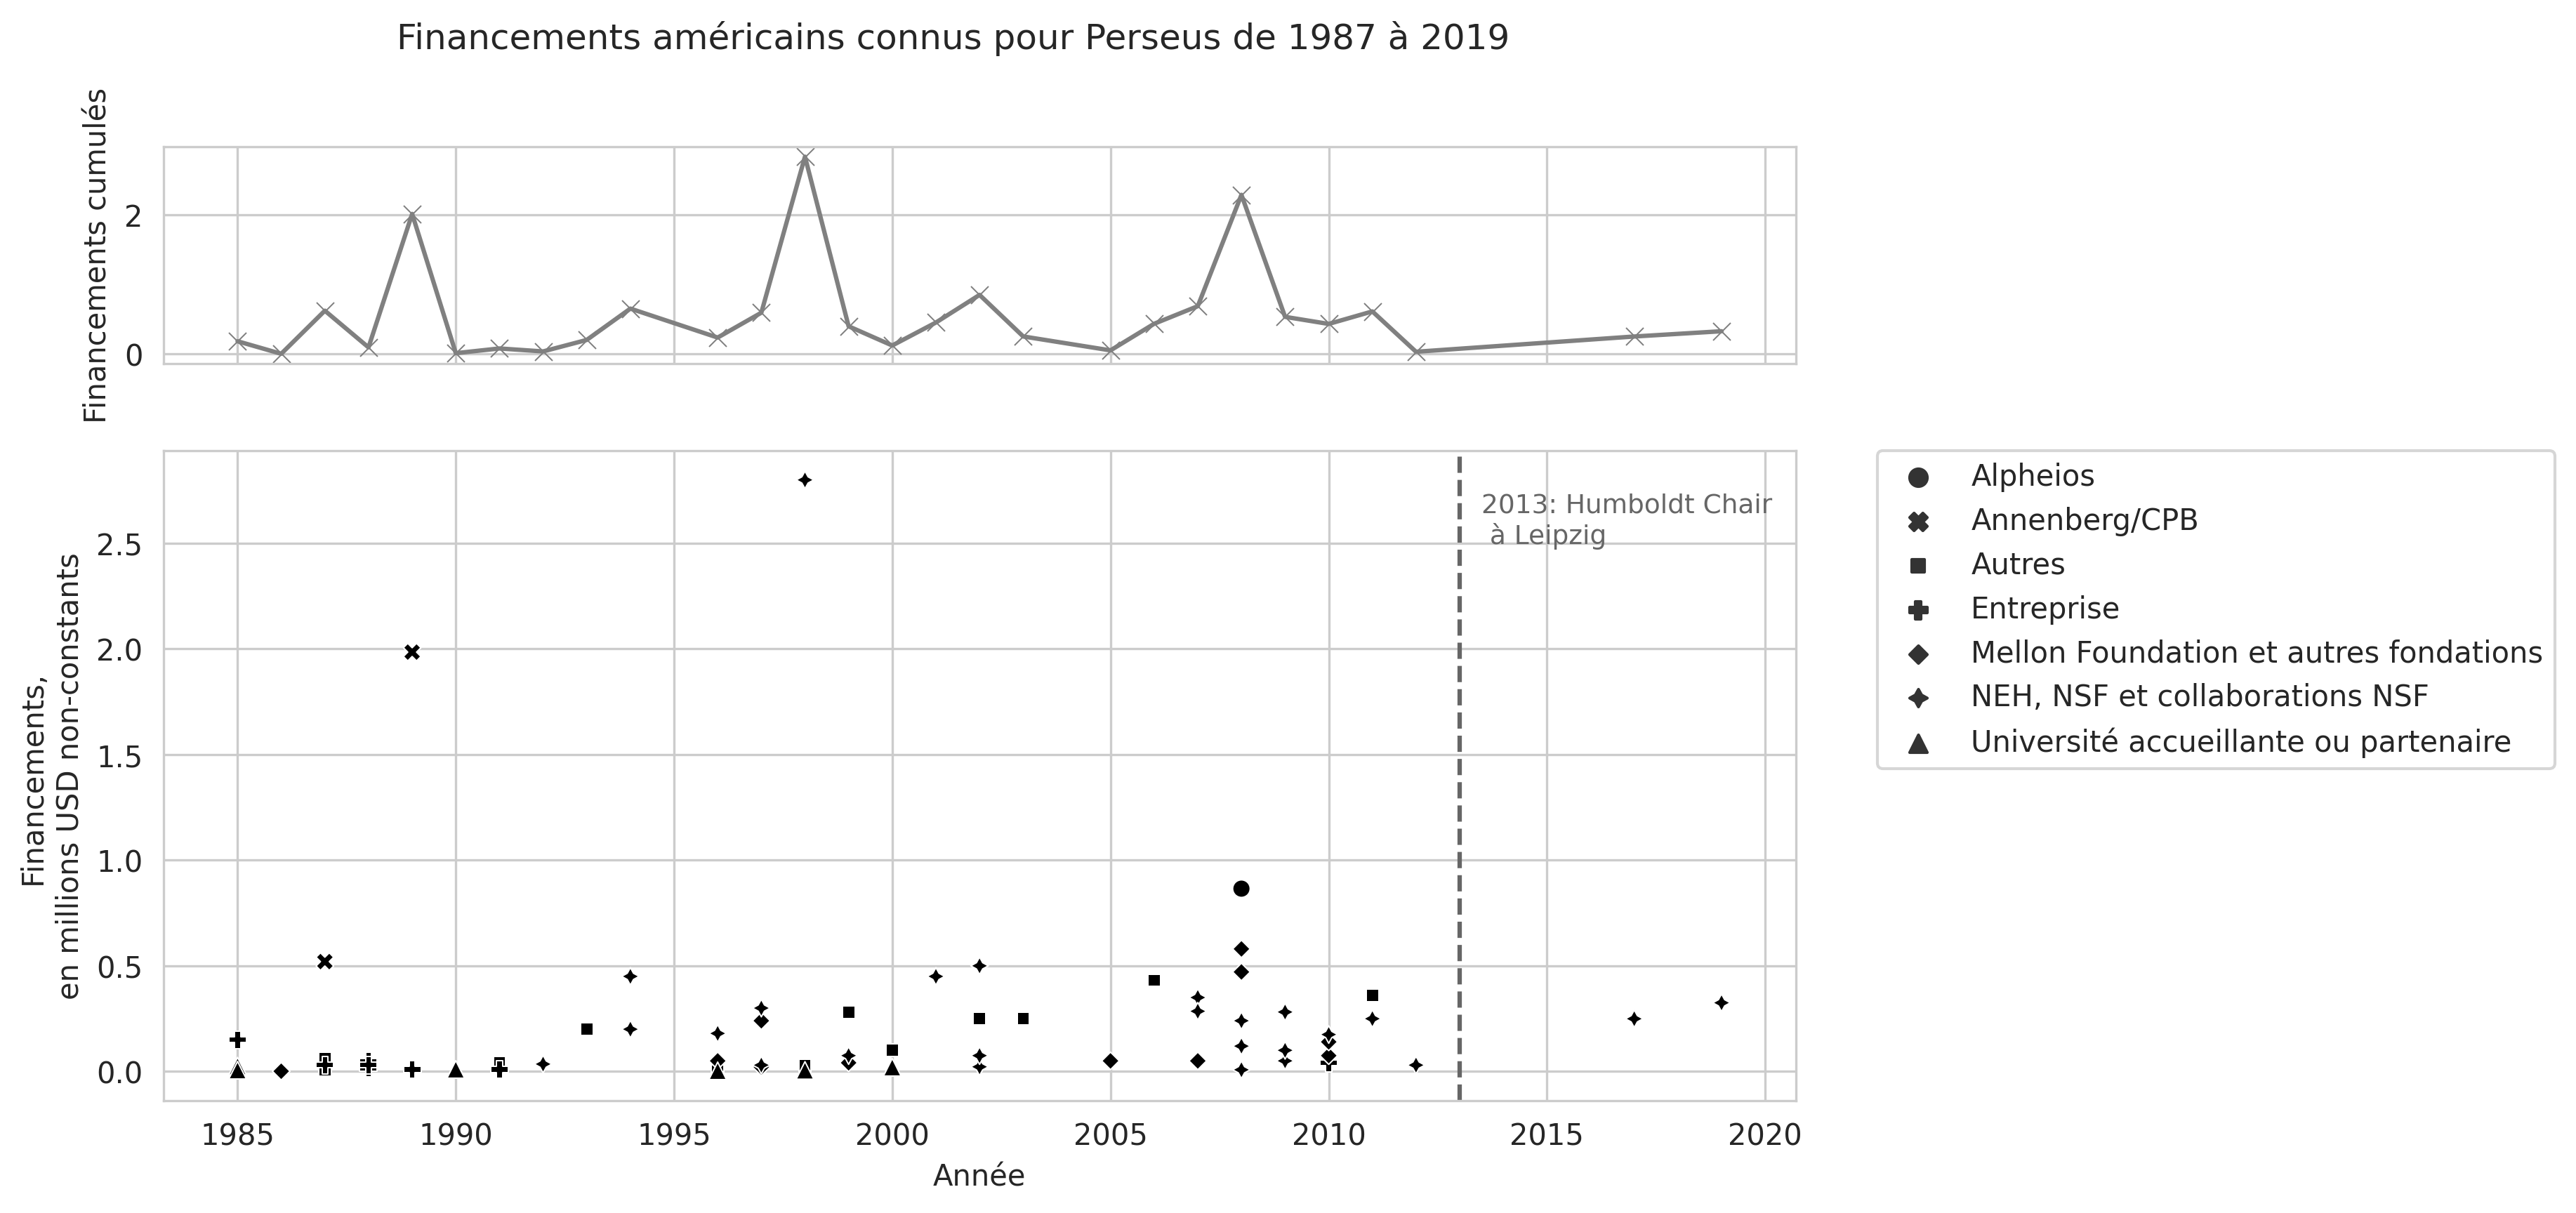
\includegraphics[width=\linewidth]{figures/chap1/part1/PerseusFinancements.png}
    \caption{Financements américains connus de Perseus, en millions de dollars non constants, d'après les pages \textit{Grants} de Perseus, le CV de G.~Crane et les archives de la Mellon Foundation et de la NEH. On distingue clairement trois vagues (1: fondation, 2: web, 3: expansion) et l'exportation de Perseus vers l'Allemagne pendant quelques années pour un retour après la fin des financements à partir de 2017.}
    \label{fig:chap1:perseus_fundings}
\end{figure}

Au milieu de la décennie 2000, la fin du financement \textit{A Digital Library for the Humanities} et un ensemble d'autres financements permettent la sortie d'une nouvelle version majeure\footcite{noauthor_gregory_nodate}, la 4.0. La 3.0 ayant subi de nombreuses modifications suite aux besoins émergents de l'ensemble des financements de la seconde phase, son code n'est plus maintenable. La 4.0 est une remise à plat complète du projet Perseus avec un passage vers le langage Java pour le fonctionnement du site, le passage au XML \acrshort{tei} P4 pour ses ressources textuelles et la mise à disposition pour la première fois de ces dernières en téléchargement libre. Ce changement structurel du \textit{backend} s'opère en 2005, suivi d'une mise sous licence \textit{Creative Commons} de ses sources en 2006 et de son code en \textit{open-source} en 2007\footcite{rockwell_face_2013}. Cette troisième phase marquée par la 4.0 voit l'expansion de Perseus dans le domaine textuel se confirmer: à partir de 2000, aucun financement ne concerne la partie archéologique ou visuelle de Perseus, tandis que se développent une bibliothèque sur la guerre civile (2003), une extension pour les textes arabes (2006), le traitement des entités nommées (2007) ou de la grammaire grecque par \textit{treebank} (2008), etc. Les corpus ont grossi, toujours dans un objectif de mise à disposition des traductions\footnote{Avec comme seule source notre expérience pour le projet Perseus, des statistiques de 500~000 visites sur le site par semaine nous sont parvenues.}. En 2013, alors que G.~R.~Crane obtient la ``chaire Humboldt pour les Humanités Numériques'' à Leipzig, la troisième phase s'éteint, et peu de financements sont obtenus du côté américain, malgré une attache conservée à Tufts.

Un phénomène nouveau accompagne cette apparition du web dans les foyers et bibliothèques: la naissance de corpus produits par des non-spécialistes, transformation numérique de ce que l'érudition locale et les sociétés savantes produisaient et produisent en papier, avec la mise à disposition par l'effort de particuliers hors du monde académique de documents, données ou analyses scientifiques. Trois corpus existants encore en 2021 naissent sur la période 1995-1998: \textit{Curculio}\footcite{hendry_curculio_1995}, \textit{LacusCurtius}\footcite{lomarcan_lacuscurtius_1999} et \textit{The Latin Library}\footcite{carey_latin_1998} (1998). Les trois se concentrent en particulier sur la problématique des textes latins, et pour cause, ni Perseus ni \acrshort{phi} ne fournissent alors ces corpus. Ils sont rejoints par des projets francophones dans la décennie 2000, qui correspond à l'explosion de l'accès au web en France et en Europe: \textit{Remacle.org} arrive en 2003\footcite{philippe_remacle_site_2008}, \textit{Latin, Grec, Juxta} de Gérard Gréco en 2006\footcite{gerard_greco_latin_2006}. La particularité des sites francophones tient en la carrière professionnelle de leurs fondateurs: tous deux sont professeurs de lettres classiques de formation. Quelle que soit la situation professionnelle de ces créateurs de contenu, ils partagent tous la particularité de réaliser ces projets sans financement propre, en dehors des cadres universitaires, avec parfois une exhaustivité particulièrement importante, comme pour \textit{The Latin Library}, et avec une véritable focalisation sur le latin.

\subsubsection{Les projets nés sur le web}

La fin des années 1990 et la première décade des années 2000 voient aussi l'émergence de projets nouveaux, cherchant à installer durablement dans le paysage numérique les lettres classiques. Si nous en parlons peu, car nous ne les utiliserons pas dans notre recherche, les premiers à se développer sur le web sont de loin les projets épigraphiques, dont plus d'une vingtaine est déjà répertoriée par Tom Elliott pour le compte de la société américaine d'épigraphie latine et grecque en juillet 1998\footcite{elliott_links_1998}. Mais les projets littéraires s'intéressent aussi à la toile et y naissent.

Le premier mouvement de ces projets nés sur le web est celui de projets qui resteront au niveau du HTML: des sites pour lire des textes, donner accès à ces derniers avant tout. En 1996, par exemple, naît la \textit{Bibliotheca Augustana} d'Ulrich Harsch\footcite{harsch_bibliotheca_nodate}, dont il nous est malheureusement impossible de retrouver le contenu original. En 1998, c'est au tour d'\textit{Itinera Electronica} d'apparaître. Elle est construite autour de deux axes: un ensemble de cours (sur quatre niveaux: acquisition, maîtrise, transmission et approfondissement) et de ressources textuelles dont la mise en ligne ne semble remonter qu'à 2002, d'après les journaux du site\footcite{meurant_itinera_nodate}. La \textit{Roman Law Library} sort en 2001: il est produit par des historiens du droit, hors du domaine des lettres classiques, fruit d'une collaboration internationale, et cherche à couvrir ``depuis les premiers textes de l'époque royale jusqu'aux compilations de la période byzantine''\footcite{lassard_roman_2001}. Les corpus naissent peu à peu aux États-Unis et en Europe, en latin comme pour les autres langues. Leur catalogue est complexe à construire tant le passage du temps fait disparaître ces corpus\footnote{Le peu de références faites dans les ouvrages ou articles scientifiques n'aident pas à en conserver la trace.}. Les outils de développement web sans apprentissage du code font leur apparition, les compétences intègrent les institutions peu à peu. En 1995 sort \textit{Vermeer Frontpage}, renommé \textit{Microsoft FrontPage} en 1996, qui permet le développement de site web sans compétences avancées en programmation, via une interface graphique. Dès 1997, on voit émerger de guides\footcite{la1997guide} à destination des non-spécialistes des communautés éducatives. Un projet de bibliothèque numérique de ressources slaves fait clairement mention de l'usage de \textit{FrontPage} dans son élaboration\footcite{deyrup1998character} et celle de son corpus, tandis que d'autres, tel le projet \textit{Journeys in Time 1809-1822} à l'université de Macquarie (Australie), rejettent son usage pour la production d'un code ``plus propre''\footcite[p.~41]{10.3316/informit.752609435027594}. Dans la plupart des cas précédemment mentionnés, ils survivent -- c'est ainsi qu'on les connait aujourd'hui -- et se sont enrichis, mais ne sont jamais sortis du contexte des sites web statiques, précompilés en HTML.

La fin 1990 et surtout le début 2000 voient des innovations majeures dans le monde du développement web et de la gestion de corpus électroniques. D'abord, les bases de données SQL (notamment les serveurs MySQL) et le langage PHP voient le jour et dominent rapidement le monde du développement amateur, tout en se faisant parallèlement une place dans le monde du développement professionnel\footnote{Malgré nos recherches, nous n'avons pas trouvé d'autres sources sur ce sujet que celles que nous citons. Et pourtant, le début des années 2000 voit l'émergence de sites à tutoriel comme celui du \textit{Site du zéro}, la réduction des prix pour l'hébergement de sites, la naissance (et la mort) des salons de discussions pour l'entraide qui favorisent clairement la formation en autodidacte d'une nouvelle génération de développeurs. C'est en tout cas notre expérience de ces années-ci.}. Associés aux serveurs Apache\footcite{smith_lamp_nodate}, faciles à mettre en place pour les hébergeurs comme Free en France et d'autres, il devient facilement possible de déployer des sites dynamiques à bases de données relationnelles avec une formation rapide à la programmation. Des outils de publication (\acrlong{cms}) faciles à installer voient le jour et accompagnent ce mouvement technologique\footcite{purer_php_nodate}. Parmi ces applications plus complexes, on notera l'apparition entre autres de \textit{Musisque deoque}\footcite{gelderblom_musisque_2008}. Dans son compte-rendu, Werner Gelderblom indique qu'il s'agirait du premier corpus -- il parle d'archive -- à intégrer les variantes et l'apparat critique\footnote{``\textit{The important innovation of MQDQ is that it is the first large-scale archive to include [apparatus] for a growing number of texts, and that it also provides effective search tools for them}'', \cite[p.233]{gelderblom_musisque_2008}}. D'autres projets similaires se développent: ils sont fondés sur des bases complexes, avec des technologies \enquote{avancées} comparativement à du pur HTML, comme le CGL\footcite{garcea_corpus_2010}. Ce dernier montre par ailleurs l'inconvénient de cette nouvelle couche de complexité: si \textit{MQDQ} est encore en ligne aujourd'hui, le \textit{Corpus Grammaticorum Latinorum} a complètement disparu\footnote{Une nouvelle version est prévue depuis quelques années.}; l'hébergement de simples fichiers HTML et celui d'applications complexes et dynamiques ne posent pas les mêmes défis.

Les années 2000 sont aussi celles de l'adoption par les \textit{guidelines} TEI du XML, d'abord avec la TEI P4 en 2001, puis avec la TEI P5 en 2007. La technologie prend de plus en plus de place dans plusieurs champ universitaires, la liste des participants au meeting de 2003 montre par exemple cette belle diversité de domaines\footnote{\url{https://tei-c.org/Vault/MembersMeetings/2003-info/mm22.html}}. En 2007, une étape supplémentaire est passée: la portée de la réunion annuelle de la TEI change de forme, passant du nom \textit{annual members meeting} à celui d'\textit{annual conference}, on ne publie plus la liste des participants à cette réunion, laissant penser qu'elle est de toute façon trop lourde pour être publiée\footcite{noauthor_members_nodate}. S'il n'a pas fallu attendre ces changements organisationnels pour que la grammaire TEI soit une promesse attirante, ils en sont autant d'indices de son adoption croissante par une grande variété d'individus et d'institutions. Dès 2001, T.~Nellhaus dresse le portait d'un outil pouvant révolutionner les bibliothèques dans leur mise à disposition de corpus grâce à la standardisation qu'elle implique: pour l'auteur, sa souplesse et sa capacité d'encoder des faits précis représentent une opportunité, bien qu'il ne soit pas sans défauts\footcite{nellhaus_xml_2001}. Dès 2002, l'\acrfull{ehess} via le laboratoire en médiévistique  \acrfull{ciham} à Lyon adopte la TEI pour l'édition de sermons et d'autres projets à travers les figures tutélaires de Marjorie Burghart et Nicole Dufournaud\footcite{burghart_edition_2011}. Dès 2002 aussi, l'\acrfull{enc} adopte via sa cellule numérique le standard\footcite{poupeau_les_2006}. Chacune de ces institutions évoque la même raison: la TEI, à travers son encodage fin de phénomènes divers (linguistiques, historiques, littéraires, etc.), est un langage pivot permettant de nombreuses sorties et interprétations dont le HTML de lecture -- reproduisant presque les limites de l'imprimé augmenté des liens hypertextes -- n'est qu'une vue. C'est la même raison qui permet à G.~Crane de crier victoire quelques années plus tôt au sujet du passage de Perseus au web.


Dans le monde des lettres latines antiques, peu de projets adoptent dans un premier temps cette technologie, en dehors de Perseus qui avait parié dessus dès la fin des années 1980.  D'une part, il existe le projet \textit{Hyperdonat}. Il est à notre connaissance la première et seule édition scientifique d'une œuvre latine littéraire classique ou tardive raisonnablement longue\footnote{Il existe quelques extraits ici et là, ou quelques œuvres courtes comme le texte de Calpurnius dont nous parlons plus bas.} à utiliser le média web et des sources TEI\footcite{bureau2008hyperdonat}. L'usage de cette technologie est d'ailleurs justifié par Bruno Bureau comme le seul moyen d'éditer la base de données que représentent les commentaires de Donat, loin de l'édition d'un texte linéaire que serait celui d'un Victor Hugo par exemple\footcite[La comparaison est la nôtre.]{chaire_de_recherche_sur_les_ecritures_numeriques_exemple_2018}. D'autres tentatives existent, mais même des initiatives aussi prometteuses que la \acrfull{ldlt}, cherchant à simplifier et promouvoir l'édition critique de textes en TEI, n'arrive à proposer qu'une seule édition de texte (Calpurnius) après des années de mise en place. Comme le note d'ailleurs le porteur de ce projet, Samuel J.~Huskey, en 2019, ``les vraies éditions critiques sur internet sont encore rares''\footnote{``\textit{truly critical editions on the internet are still rare}'', \cite{huskey_digital_2019}}. De l'autre côté du spectre des projets en TEI, hors des objectifs d'éditions critiques, se trouve aussi le projet italien de la  \textit{Latin Digital Library of Late Antiquity} (DigilibLT)\footnote{\textit{Biblioteca digitale di testi latini tardoantichi}, d'où le LT.} dont l'objectif est de produire un nouveau corpus de textes tardifs, absents de Perseus, sans pour autant en proposer de nouveaux établissements de texte. À partir d'éditions imprimées globalement plus récentes que celles de Perseus, plutôt issues de la période 1950-2000, elle propose une collection cataloguée de textes sur la période du deuxième au huitième siècle, incluant des textes impossibles à trouver ailleurs sous format numérique, comme des traités de médecine et de gynécologie. \textit{DigilibLT}\footcite{lana_metodologie_2012} prend par ailleurs le même chemin que celui du projet \textit{Perseus} en affirmant l'importance du caractère \textit{open access} et libre de son projet, dont le corpus est téléchargeable dès sa fondation\footnote{Dans son article, Maurizio Lana titre une de ses parties ``\textit{Accesso aperto, licenze Creative Commons, software libero}'' (fr. Accès ouvert, licence Creative Commons, logiciel libre). \cite{lana_metodologie_2012}}. Mais le monde de la TEI latine classique et tardive s'arrête là, du moins pour les œuvres ``littéraires'' (on inclut les traités de médecine): l'épigraphie a -- elle -- bien adopté l'usage de la TEI et de sa variante Epidoc\footcite{elliott2007epidoc} pour la publication de ces corpus de textes\footcite{bodard2007inscriptions,cayless2010epigraphy}.

\subsubsection{OCR et corpus de masse}

La littérature classique en accès ouvert commence à être bien couverte: il reste quelques textes impossibles à trouver en format numérique , comme les \textit{Declamationes Minores} de Quintilien ou les auteurs fragmentaires, mais ils restent marginaux. Du côté de la littérature tardive, entre DigilibLT, la \textit{Patrologia Latina} et le CSEL, la couverture tend à être meilleure, même si de nombreux textes ne sont pas édités ou ne sont tout simplement pas encore tombés clairement dans le domaine public\footnote{La question du droit d'auteur sur les éditions de textes anciens est complexe, spécifique à chaque territoire, y compris en Europe, et pose de vrais problèmes d'interprétations, dont certains producteurs de corpus se plaignent, comme Philipp Roelli dans \cite{roelli2014corpus}. Sur le plan national, de nombreuses publications existent, comme \cite{combalbert_lediteur_2015, demonet_confiscation_2018}. Sur le plan international, et celui des textes latins \cite{fischer2017digital, dillen_digital_2016}. Sur des textes plus récents, \cite{dusollier_international_2019}}. Au contraire, les littératures médio-latine et néo-latine sont particulièrement absents des corpus en ligne, et leur mise à disposition tarde. Dans ce contexte, l'idée de recourir à des dépôts massifs de numérisations photographiques émerge pour élaborer de nouveaux outils ou offrir de nouvelles approches des textes.

En 2011 et 2012, David Bamman, avec G.~Crane\footcite{Bamman:2011:MHW:1998076.1998078} puis avec David Smith,\footcite{bamman_extracting_2012} s'intéresse pour la première fois à un corpus en friche: celui des campagnes de numérisation, majoritairement privées dans son cas précis, et du résultat de la reconnaissance optique de caractères (\acrshort{ocr}) appliquées à ces documents. Il dénombre, en 2012, 27~014 textes catalogués comme latins dans l'index du projet \textit{Internet Archive}, comprenant tout autant les classiques latins que les thèses et autres ``commentaires de la philosophie d'Hegel'' produits en Allemagne, mais écrits en latin au dix-neuvième siècle\footcite{bamman_extracting_2012}. Puis, en triant les données, en partie manuellement\footcite{bamman_dbammanlatintexts_2018}, il obtient une liste de plus de onze mille ouvrages comprenant environ 1,38 milliard de mots\footnote{Ce chiffre est à prendre avec une certaine précaution: la méthode de calcul des mots n'est pas précisée et la définition de ce qu'est un mots ici non plus.}. Au moyen des données récupérées, il met à disposition les premiers \textit{embeddings}\footnote{\textit{Cf.} Chapitre 2, \textit{Embeddings}.} massifs de l'histoire du latin approché. Cependant, ses données sont problématiques: d'une part, la méthode de vérification manuelle du catalogue n'est pas expliquée; d'autre part, le résultat final contient des documents dont l'\acrshort{ocr} est absolument inexploitable (``\texttt{tkei: SiiimiemfiBgMiffem mvemsfimUttrUffHk rejcijps}'' étant un des exemples de mauvaise transcription qu'il cite lui-même).

\begin{figure}
    \centering
    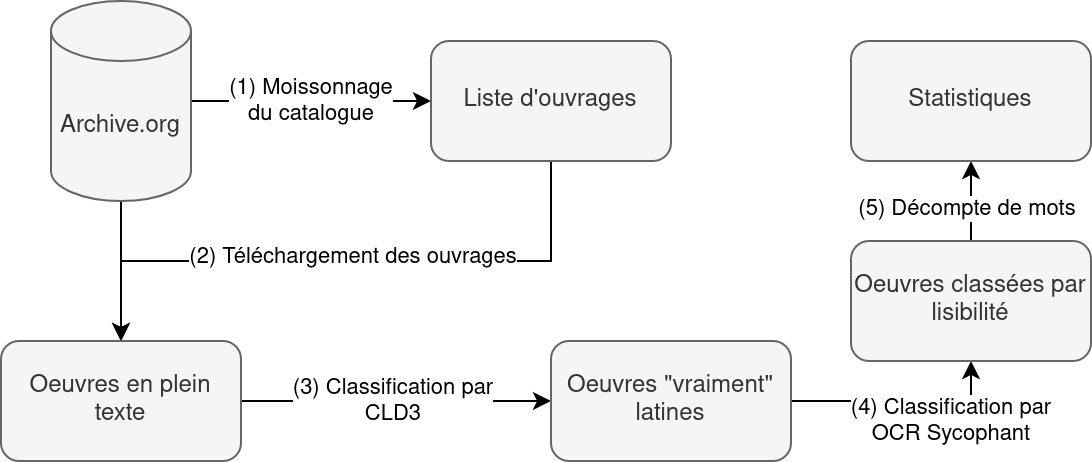
\includegraphics[width=.8\linewidth]{figures/chap1/part1/ocrSycophant.png}
    \caption{Récapitulatif de la chaîne de traitement appliquée sur Archive.org}
    \label{fig:chap1:workflow-sycophant}
\end{figure}

L'OCR ayant progressé depuis 2013, et la méthode de D.~Bamman n'étant pas totalement claire, nous nous sommes intéressé à l'évolution du dépôt \textit{Internet Archive}. Pour faire cela, nous avons traité les données de cette bibliothèque numérique en cinq étapes (reproduites en figure \ref{fig:chap1:workflow-sycophant}). Les œuvres classées comme étant en latin par l'\textit{Internet Archive} sont téléchargées. On sélectionne au hasard un quart des lignes de chacune des œuvres sur lesquelles on applique un classificateur de langue\footcite{salcianu2018compact}. 
% GABAY REPRENDRE ICI 6/01, p. 35
Ce classificateur indique des statistiques pour plusieurs langues s'il a des doutes sur cette classification: on retient alors qu'une ligne est classée comme latine si elle a un score supérieur à 60\% en latin\footnote{Ce seuil a été fixé pour prendre en compte l'existence d'œuvres bilingues.}. Après ce traitement, on applique un outil conçu par nos soins pour classer les lignes transcrites en terme de qualité (compréhensibles ou non), OCR~Sycophant\footcite{Clerice_OCR_Sycophant_2021}. OCR~Sycophant a été développé autour de modèles de classification classiques basés sur des n-grams, et a été entraîné à partir d'un dataset de phrases du corpus Archive.org sélectionnées aléatoirement et annotées à la main: ont été classées comme ``incompréhensibles'' les données qui n'étaient pas en latin (\textit{eg.} ``\texttt{" Mr Bryce's test, on account of the difficulty of pro-}''), qui étaient illisibles (eg. ``\texttt{"7 „ 7- f Ak. —2 vi rt*- ('wbrf-}'') ou difficilement lisibles (\textit{eg.} ``\texttt{(Hciucuto qucfo quob fwutuinlto}''), ou encore qui correspondaient à des lignes considérées comme trop courtes (\textit{eg.} ``\texttt{5}''). Ce classement effectué, on obtient un pourcentage de lignes estimées propres : on compte alors les \enquote{mots} de chaque texte (un mot étant considéré simplement comme un élément séparé par une espace).

Ce résultat donne des chiffres absolument prometteurs, tout en demandant une forme de patience. On compte dans les documents disponibles en latin presque 5~000 œuvres avec une qualité d'OCR à plus de 90\% (\textit{cf.} table \ref{tab:chap1:latin-OCR}) représentant 635 millions de mots. Si l'on ajoute à ce corpus les textes avec plus de 80\% de qualité OCR, on atteint les 1,451 milliard de mots et un peu plus de 17~000 ouvrages. Il existe probablement des doublons parmi les textes, mais un corpus de taille inégalée, en quantité et en diversité, existe dans ces dépôts: avec ces deux catégories de textes propres, on atteint près de dix fois plus de mots que les œuvres contenues dans \textit{Corpus Corporum}, et en ne prenant en compte que la bibliothèque \textit{Internet Archive}.

\begin{table}[ht]
\centering
\begin{tabular}{l|rrr}
\toprule
                               & Nombre de volumes & \% du total & Nombre de mots \\ \midrule
Qualité \textgreater 90\% OCR  & 4 946              & 23.73       & 635 201 534    \\
Qualité \textgreater 80\% OCR  & 12 169             & 58.38       & 816 236 079      \\
Qualité \textgreater 60 \% OCR & 3 709              & 17.79       & 182 697 928      \\
Reste                          & 19                 & 0.09        & N/A           \\ \bottomrule
\end{tabular}
\caption{Statistiques sur les ouvrages latins disponibles sur Archive.org au début juillet 2021}
\label{tab:chap1:latin-OCR}
\end{table}

La question de l'OCR et de sa qualité (surtout pour les œuvres imprimées avant la fin du dix-neuvième siècle), deviennent donc prépondérantes dans le contexte de l'acquisition de textes fac-similaires (et donc non édités). Le problème de la reconnaissance de texte pour les œuvres des incunables et de l'époque moderne, avec ses S longs et ses restes d'abréviations, est peu à peu réglé par la mise à disposition massive de données d'entraînements et de modèles adaptés. Dans ce cadre, le travail de Simon Gabay autour des imprimés du 17e siècle est absolument majeur et fondateur\footcite{simon_gabay_2020_3826894}: son usage a permis de générer de très bons modèles OCR\footcite{gabay:hal-02577236} et, à partir de quelques données latines\footcite{Clerice_CREMMA_16_18_Prints_2021}, permet de produire des données propres de textes latins imprimés avant le 19e siècle, de l'\textit{Utopie} de Thomas More à des œuvres en zoologie du 18e siècle en passant par l'\textit{Historia de duobus amantibus Euralio et Lucretia}, avec des taux de reconnaissance à plus de 96\%. 

Mais un autre enjeu pour la mise à disposition de texte arrive aussi à travers la Reconnaissance d'Écriture Manuscrite (REM, ou plus communément l'anglais HTR pour \textit{Handwritten Text Recognition}). La transcription automatique des documents de la pratique et des manuscrits littéraires, quel que soit leur genre, apportera une autre masse de données pour l'étude du latin sur le temps long. Le développement de cette technologie, sa popularisation par Transkribus\footcite{kahle2017transkribus}, sa mise à disposition \textit{open source} par Ben Kiessling via Kraken\footcite{kiessling2019kraken} puis eScriptorium\footcite{kiessling_escripto}, ont permis l'émergence de modèles partagés extrêmement performants. Les travaux d'Ariane Pinche sur les manuscrits en ancien français\footcite{Pinche_CREMMA_Medieval_an_2021} avec une reconnaissance des caractères supérieur à 95\% ou les travaux de Dominique Stutzmann\footcite{hazem2020books} ont montré que cette approche était prometteuse et pouvait potentiellement passer à l'échelle. Il est probable que l'étude quantitative du latin soit largement redéfinie par la mise à disposition de ces corpus nouveaux sur le moyen terme, en s'attaquant de front aux dépôts institutionnels nationaux ou régionaux, comme la Bibliothèque nationale de France et son dépôt Gallica. Dans ce cadre, des projets comme le Gallicorpora, dont font d'ailleurs partie S.~Gabay et A.~Pinche, montreront rapidement ce à quoi l'on peut s'attendre sur le court terme, avec le développement d'une chaîne de traitement pour la production de documents fac-similaires encodés finement en TEI.

Si l'approche évoquée précédemment est celle d'une approche massive, bruitée et sans réelle intervention humaine, une approche qualitative des corpus en friche est aussi possible. La révolution de la qualité des données obtenues via OCR a permis aussi de développer de nouveaux projets, comme VELUM dirigé entre autres par Bruno Bon pour la mise en place d'un corpus médiéval latin de texte OCRisés\footcite{bon2019challenges}. Du côté des périodes classiques et tardives, il faut alors se tourner vers l'initiative \acrfull{ogl} menée par G.~Crane d'abord depuis l'université de Leipzig puis de Tufts.

Né entre 2008 et 2009, \acrshort{ogl} est le fruit d'un besoin ressenti par deux enseignants et chercheurs en lettres classiques associés au \acrfull{chs} d'Harvard\footnote{Les locaux de ce dernier sont par ailleurs complètement distincts de ceux d'Harvard, au point d'être dans deux États et deux villes différentes: Cambridge, Massachusetts et Washington DC.}: Neels Smith et Christopher Blackwell\footcite{muellner2019free}. Ce projet a pour objectif de produire un corpus pour le grec intégralement \textit{open source}, gratuit et accessible, et standardisé afin de pouvoir s'assurer de la collaboration et de la réutilisation par des partenaires divers. Une première tentative de partenariat avec le TLG échoue en 2010, et pousse l'OGL se lancer dans la compilation d'un nouveau jeu de données, qui ne prendra forme qu'en 2015.

Neel Smith est un proche ami de Gregory Crane: ils ont partagé les bancs de Harvard, ont travaillé en équipe sur HCCP et les premières moutures de Perseus et ont partagé le même directeur de thèse, Gregory Nagy, directeur depuis 2000 du CHS. En 2013, Gregory Crane obtient donc la \textit{Digital Humanities Chair} à l'université de Leipzig, où il a pour objectif de relancer le projet Perseus. Dans ce cadre, ses premières décisions sont simples: il faut agrandir le corpus gréco-latin, en particulier sur le premier millénaire de notre ère, et ajouter un grand nombre de traductions. Les pères de l'Église et l'ensemble de la littérature tardive sont, au moment de ce choix, indisponibles en accès libre. Pour le latin, l'OCR a fait les progrès qui permettent à l'équipe de Perseus de mettre en place de nouveaux corpus, dont les deux premiers sont le \textit{\acrfull{csel}}\footcite{noauthor_csel_nodate} et la \textit{\acrfull{pl}} de Migne. Si la \acrshort{pl} a été introduite précédemment et existait dans des versions concurrentes, le CSEL est quant à lui un corpus d'éditions critiques des pères latins de l'Église. Née en 1864, cette initiative autrichienne toujours en cours et hébergée à l'université de Salzburg\footcite{noauthor_history_nodate} a publié depuis sa fondation plus d'une centaine de volumes comprenant potentiellement plusieurs œuvres, comme le volume 10 constitué des œuvres complètes de Sedulius Scottus (IXe siècle), et dont une partie est tombée, avec son apparat critique, dans le domaine public.

Au niveau technique, ces corpus sont transcrits automatiquement, puis corrigés et structurés en XML TEI par des entreprises spécialisées, dont l'entreprise française Jouve et sa succursale malgache. Leur XML est ensuite adapté aux attentes de Perseus par des équipes internes puis mis à disposition sur Github. C'est ce même fonctionnement qui est repris lors de la mise en place de l'alliance entre le CHS, l'université de Mount Alison et les équipes de G.~Crane. Dans l'article de L.~Muellner, on apprend que l'OCR est réalisée par les équipes de Mount Alison, sous l'égide de Bruce Robertson qui entretient des modèles pour l'OCR grecque. Les données sont envoyées ensuite à l'entreprise plurinationale \textit{Digital Divide Data} (DDD; Cambodge, Kenya, Indonésie) pour leur mise en Epidoc, grammaire XML retenue par Perseus. Le coût budgété de numérisation et d'encodage par DDD est de 50~000\$ pour quatre millions de mots, soit bien moins que les premiers projets des années 1970 et 1980. Enfin, la mise en conformité et la vérification des données sont finalement assurées par des stagiaires, étudiants de la licence au doctorat, hébergés d'abord uniquement par le CHS puis par l'université de Virginie\footcite{robertson2019optical}.

La production de l'ensemble de ces corpus a permis à Perseus de se tourner vers une nouvelle version, en partie financée par le CHS, Perseus 5\footnote{\url{https://scaife.perseus.org/}}, dont la mise à jour est automatiquement liée à l'évolution des corpus, contrairement à la version 4, et qui a été l'objet d'une refonte totale de l'infrastructure de Perseus. Cette version a abandonné -- pour le moment -- les données graphiques (archéologiques, histoire de l'art, etc.) pour ne s'intéresser qu'aux données textuelles.

Enfin, avec l'apparition de tous ces projets se pose la question de l'éclatement des corpus sur internet. Entre les données de Perseus, de DigilibLT, d'autres projets comme le \textit{Corpus Grammaticorum Latinorum} de Jussieu (CGL), l'accès à un corpus latin unifié devient problématique. C'est un problème d'autant plus important que ces sites ne partagent pas une architecture commune qui pourrait permettre de centraliser les recherches sur de multiples corpus. En 2011, Philipp Roelli, un éditeur de texte aussi intéressé par la linguistique de corpus, met en route le projet \textit{Corpus Corporum} à l'université de Zurich\footcite{roelli2014corpus}. Ce projet est très peu financé en dehors d'une aide de la chaire de latin et d'une partie des fonds de la COST-Action IS1005 dont l'objectif principal était la formalisation d'un réseau de recherche autour du latin médiéval\footnote{\textit{Corpus Corporum} est donc plus une externalité positive de cette dernière que l'un de ses objectifs.}. Ph.~Roelli le définit comme une ``meta-collection'': \textit{Corpus Corporum} ne produit pas de numérisation ou d'édition numérique, il centralise, en harmonisant, les données d'une dizaine (en 2014) puis d'une trentaine d'autres projets (en 2021), accumulant ainsi en un seul lieu presque 164 millions de mots à la fin 2021 représentant toutes les périodes du latin, du classique au néo-latin. Bien que techniquement ``rustique'' du côté client\footnote{L'usage des \textit{iframes} a presque complètement disparu du web, hormis sur \textit{Corpus Corporum}.}, le projet a l'avantage d'être rapide, facile d'usage -- à l'image de \textit{The Latin Library} -- et de permettre l'accès à des corpus perdus comme les CGL, indisponibles sur leur site d'origine depuis quelques années.

Après l'avènement du micro-ordinateur et du web, les corpus latins ont ainsi évolué pour atteindre aujourd'hui une ouverture sans commune mesure. Pour les plus grands classiques, il est possible d'en trouver des éditions voire des traductions -- en anglais majoritairement -- assez facilement en plein texte. Et quand cela n'est pas possible, on peut toujours faire recours aux dépôts institutionnels ou privés tels qu'Archive.org ou HathiTrust aux États-Unis afin d'obtenir la numérisation d'un de ces ouvrages. Cette révolution, sur presque cinquante ans, est celle de l'accès aux textes latins classiques et tardifs dans leur intégralité -- ou presque -- et de manière gratuite, permettant ainsi de produire de nouveaux questionnements et de développer de nouvelles approches.

\section{Constitution d'un corpus de sources littéraires latines}

Après cinquante ans de compilations et de production de textes numériques, le nombre de corpus disponibles -- qu'il soient ouverts, fermés ou à réutilisation limitée -- est assez important pour permettre une recherche plein texte ou la production d'exempliers numériques. Le travail de Ph.~Roelli montre que, en produisant des corpus ouverts et ré-exploitables, les projets comme \textit{Perseus} et \textit{DigilibLT} ont constitué des gisements de textes analysables, indexables et réutilisables dans un contexte autre que celui d'une lecture linéaire et ``manuelle''. Pour notre recherche, nous aurons besoin d'un corpus permettant d'effectuer des recherches plein texte, d'extraire des exemples. Beaucoup d'options s'offrent à nous pour constituer ce nouveau meta-corpus, de l'utilisation d'outils commerciaux comme la \acrshort{llt} à celle de corpus en friche de l'\textit{Internet Archive}. C'est pourquoi il semble primordial de construire notre méta-corpus autour de principes, que l'on appelle généralement \enquote{bonnes pratiques} ou éthique, guidant ensuite la compilation ou réutilisation d'un tel corpus. 

Nous décrirons dans un premier temps ces principes et ce qui les rend indissociables de la création de corpus. Dans un second temps, nous présenterons les choix techniques, la méthode de compilation du meta-corpus et le résultat de cette dernière. Enfin, nous étudierons l'impact que peut avoir l'un des choix techniques effectué, à savoir le choix d'avoir un corpus plus petit mais dont la structure de citation est \textit{machine actionable}.

% ToDo: A RÉÉCRIRE car le plan à changer
% Nous étudierons ensuite l'importance de l'encodage fin de textes et de l'impact que son manque peut avoir sur la production de savoir via des analyses statistiques. Enfin, nous discuterons de la compilation du corpus effectuée à partir de l'œuvre scientifique de J.~N.~Adams, des limites de cette dernière, mais aussi des méthodes employées pour compiler cette collection.

\subsection{Objectifs et prérequis d'un corpus pour une analyse automatisée}

\begin{quote}{J.-B.~Camps}
\enquote{La distinction entre humanités « numériques » et « computationnelles » est dans l’air. Au‑delà d’un pur choix terminologique distinctif ou d’un retour aux \textit{humanities computing} du XXe siècle, la revendication d’une dimension computationnelle rend compte d’un basculement, à mon sens éminemment souhaitable, d’une perspective tournée vers la diffusion et la publication électronique, à un accent mis sur les données et leur exploitation pour la création de nouveaux savoirs scientifiques.}\footnotemark
\end{quote}
\footnotetext{\textcite{camps_ou_2018}}

Le constat de Jean-Baptiste Camps est juste: depuis les années 2000 et 2010 en particulier, la technicisation de l'analyse des documents et des sources, à travers l'explosion de l'usage de la stylométrie par exemple, et le besoin d'une reconnaissance à part de cette technicisation a donné lieu à de nouvelles sous-communautés des humanités numériques, avec leurs réseaux parallèles de conférences. En juillet 2019, à la suite de la conférence annuelle de l'\acrfull{adho}, association internationale principale des humanités numériques\footnote{Cette association, l'\acrshort{adho}, organise à ce moment-là DH2019 à Utrecht.}, un groupe d'intervenants décide de remédier à cette frustration. Quelques semaines plus tard, un sondage est publié, et son phrasé d'introduction est clairement revendicatif: \enquote{Malgré l'essor indéniable de ce nouveau domaine de recherche [les humanités computationnelles], de nombreux chercheurs estiment qu'il n'existe pas d'endroit approprié, axé sur la recherche, pour présenter et publier leurs travaux informatiques sans perdre de vue les questions relatives aux sciences humaines\footnote{\enquote{\textit{And yet, despite the undeniable growth of this new research area, many scholars still feel that there is no suitable research-oriented venue to present and publish their computational work that does not lose sight of questions relevant to the humanities.}}\textcite{noauthor_computational_nodate}}.}. Suite à cet appel de ce qui se nomme alors la CoHuRe (\textit{Computational Humanities Research}, plus tard CHR), on voit l'émergence de \enquote{contre conférences DH} avec la CHR 2020 puis 2021, ou encore des événements encore plus spécialisés comme NLP4DH\footcite{noauthor_workshop_nodate}. Si la reconnaissance du travail d'analyse technique est importante, nous différons sur l'apparente exclusion mutuelle qu'opèrerait ce \enquote{nouveau} paradigme de la recherche numérique. Dans un champ éminément protéiforme comme les humanités numériques, que l'on peut définir comme une \enquote{science auxiliaire des sciences humaines}\footnote{À l'image des \enquote{sciences auxiliaires de l'histoire}, que sont par exemple la paléographie et la numismatique.}, il faut trouver un équilibre, un balancement, plus qu'un \enquote{basculement}, entre le travail de génération de données, fruits d'un travail de recherche, et celui d'analyses. La production de corpus, de la collecte de textes\footnote{Ou d'autres types de données: ce constat est le même pour les annotations linguistiques par exemple.} pré-existant à leur édition en passant par leur contrôle qualité, est une mission qu'il ne faut pas négliger dans une approche plus ``computationnelle'' des sciences humaines, sans quoi les humanités computationnelles ne sont plus des humanités, mais de l'informatique appliquée.

\subsubsection{Le choix d’un corpus \textit{open source}: traçabilité des textes et reproductibilité}

Sans redéfinir ce qu'est un corpus, il est intéressant de s'arrêter un temps sur les définitions des deux dictionnaires français les plus populaires, \textit{Le Robert} et le \textit{Larousse}\footnote{Version en ligne de décembre 2021.}, pour questionner les traits qui caractérisent notre objet. \textit{Le Robert} définit le corpus comme un ``Ensemble fini de textes choisis comme base d'une étude.'' tandis que le \textit{Larousse} prend -- par un heureux hasard -- l'exemple des corpus grecs pour appuyer sa première définition: ``Recueil de documents relatifs à une discipline, réunis en vue de leur conservation : Corpus des inscriptions grecques.'' et rejoint légèrement le \textit{Robert} pour sa seconde (``Ensemble fini d'énoncés écrits ou enregistrés, constitué en vue de leur analyse linguistique.''). Si les deux dictionnaires se rejoignent sur un point --  à savoir, le corpus est une collection de documents, potentiellement de textes --, ils évoquent deux finalités différentes. 

La première, la conservation -- sous-entendue la maintenabilité et l'accessibilité en un même endroit, physique ou numérique, d'un ensemble documentaire -- n'est mentionnée que par le \textit{Larousse}. Dans son article de 2013, Alex H.~Poole fait le constat que ``les humanités numériques pivotent autour des données''\footnote{``\textit{The digital humanities pivot around data.}''\cite{poole_now_2013}} mais aussi que ces dernières, au format numérique, sont ``notoirement fragiles, d'une courte espérance de vie, et faciles à manipuler sans laisser forcément de traces, rendant la fraude difficile à détecter [..., sachant que] la plupart des données collectées ne sont ni organisées ni publiées''\footnote{``\textit{Our Cultural Commonwealth} report characterized digital data as “notoriously fragile, short-lived, and easy to manipulate without leaving obvious evidence of fraud”. Worse, much collected data were neither curated nor published whatsoever;'', \cite{poole_now_2013} citant \cite{unsworth2006our}}. Nous partageons ce constat -- la capacité de conservation d'un corpus doit être intrinsèque à ces derniers -- et établissons ce point comme premier objectif autour de notre corpus. 

La seconde finalité évoquée est celle de l'analyse (``la base d'une étude'', ``en vue d'une analyse linguistique''). Si nous estimons que cette finalité peut être déplacée (le corpus peut être compilé pour qu'une tierce personne s'en empare), elle est bien évidemment centrale dans notre projet. Et elle demande ainsi de définir l'objectif de notre corpus, car celui-ci définira la forme, l'outillage et les informations nécessaires à y retrouver. Nous reviendrons plus tard sur l'impact qu'a cette finalité sur le corpus, dans son annotation et sa documentation (\textit{cf.} \ref{chap1:method-annotation}).

Il faut cependant ajouter à la notion de corpus développé plus haut d'autres caractéristiques, dont celles de son ouverture, en droit et en accès. A.~H.~Poole la mentionne partiellement dans la citation avec la question de la ``fraude'', mais la position de Borgman\footcite{borgman2012conundrum}, reprise par J.-B.~Camps\footcite{camps_ou_2018}, est à notre sens assez complète. D'après elle, un corpus doit être ouvert pour
\begin{enumerate}
    \item reproduire ou vérifier la recherche,
    \item rendre les résultats d'une recherche publique disponible pour le public,
    \item permettre à d'autres de poser de nouvelles questions aux données
    \item avancer l'état de la recherche et de l'innovation.\footnote{``(1) to reproduce or to verify research, (2) to make results of publicly funded research available to the public, (3) to enable others to ask new questions of extant data, and (4) to advance the state of research and innovation.''\footnote{\cite{borgman2012conundrum} chez \cite{camps_ou_2018}}.}
\end{enumerate}

La question de la reproductibilité, par l'ouverture du corpus et sa documentation, est centrale pour Borgman, Poole et Camps. Si la traçabilité des sources n'est pas une nouveauté pour les lettres et l'histoire -- la citation de ces dernières est extrêmement codifiée afin d'être compréhensible et exhaustive, la transcription des sources de la pratique est souhaitée pour les publications scientifiques --, la reproductibilité des expériences est définitivement nouvelle. D'abord, la notion de recherche expérimentale en lettres comme en histoire est globalement nouvelle, bien qu'elle ne le soit pas nécessairement partout dans les sciences humaines. Ensuite, car la notion de reproductibilité est tout autant complexe dans le monde des sciences dites dures. Comme le dit J.-B.~Camps, ``au fur et à mesure que l’analyse de données prend de l’importance dans la constitution de nouveaux savoirs, le besoin se fait plus criant de vérifier l’intégrité des données, de reproduire les expériences, de vérifier ou infirmer les énoncés qui en découlent.''\footcite{camps_ou_2018}. L'arrivée de ces questionnements scientifiques et la "crise de la reproductibilité" en 2000, que mentionne J.-B.~Camps est suivie peu à peu par une crise en intelligence artificielle\footcite{hutson2018artificial}, traitement automatique des langues\footcite{belz2021systematic} et en histoire computationnelle\footcite{eijnatten_big_2013}.

L'ouverture des corpus rend aussi possible leur analyse et l'analyse de leurs biais, permettant d'aller plus loin que la simple reproductibilité des expériences effectuées. En accumulant des données dont on essaie de tirer des analyses ou même simplement des faisceaux d'indices, la possibilité d'introduire, inconsciemment, des biais de corpus\footnote{Un biais de corpus correspond à toute particularité du corpus liée à sa constitution qui privilégierait une période, un genre, un auteur, etc. \textit{Cf.} en archéologie la définition des biais de corpus, répartis en biais géographiques et méthodologiques: \textcite[p.~144]{resch:tel-03218240}} et -- à travers eux -- d'établir des conclusions invalides est un danger éminemment connecté aux corpus fermés. Les conséquences peuvent être importantes dans le domaine de l'intelligence artificielle, le \textit{machine learning} ne pouvant apprendre que ce qu'on lui montre. L'exemple le plus connu des dernières années est celui de la reconnaissance d'image de Google, qui, en 2019, avait tout simplement catégorisé des personnes afro-américaines comme gorilles, probablement suite à un problème de données d'entraînement\footcite{lohr2018facial, chokshi2019facial}. Si les conséquences pour notre corpus ne pouvaient être aussi graves et socialement problématiques, il reste que la question du biais est à prendre en compte. Il ne s'agit pas de promettre l'exhaustivité ni la représentativité de ce qui existe ou a existé: le domaine des lettres classiques a depuis longtemps admis la partialité -- dans les deux sens -- de ses sources ainsi que les pertes de nombreuses autres sources. Sur ce sujet, nous reprendrons l'exemple de l'article de I.~D.~Raji \textit{et al.}\footcite{raji2021ai}:

\begin{quote}{\textcite{raji2021ai}}
    \enquote{Dans le livre d'histoires pour enfants \textit{Sesame Street}, ``Grover and the Everything in the Whole Wide World Museum''[Stiles et Wilcox, 1974], le monstre \textit{Muppet Grover} visite un musée qui prétend présenter "tout ce qui existe dans le monde entier". Des exemples d'objets représentant certaines catégories remplissent chaque pièce. Plusieurs catégories sont arbitraires et subjectives, notamment les salles d'exposition des "choses que l'on trouve sur un mur" et de "la salle des choses qui peuvent vous chatouiller". Certaines sont étrangement spécifiques, comme "La salle des carottes", tandis que d'autres sont inutilement vagues comme "La grande salle". Alors qu'il pense avoir vu tout ce qu'il y a, Grover arrive à une porte intitulée "Tout le reste". Il ouvre la porte et se retrouve dans le monde extérieur.\footnote{\textit{``In the 1974 Sesame Street children’s storybook Grover and the Everything in the Whole Wide World Museum [Stiles and Wilcox, 1974], the Muppet monster Grover visits a museum claiming to showcase “everything in the whole wide world”. Example objects representing certain categories fill each room. Several categories are arbitrary and subjective, including showrooms for “Things You Find On a Wall” and “The Things that Can Tickle You Room”. Some are oddly specific, such as “The Carrot Room”, while others unhelpfully vague like “The Tall Hall”. When he thinks that he has seen all that is there, Grover comes to a door that is labeled “Everything Else”. He opens the door, only to find himself in the outside world.''}}}
\end{quote}

Tout comme l'idée d'un musée du monde entier est absurde, l'absence de biais dans un corpus l'est tout autant. Mais la possibilité de les décrire et de les vérifier à travers un corpus ouvert est primordiale pour la critique des résultats.

Nous ajouterons cependant une dernière possibilité derrière l'ouverture de ces données, particulière à leur dimension numérique: l'\textit{open access} et l'\textit{open source} dans ce contexte permettent aussi la croissance et la modification des données sur le long terme, ne figeant pas le corpus à un instant T (bien qu'il soit important de pouvoir revenir à ce dernier pour la reproductibilité). Le corpus de notre recherche doit non seulement survivre à sa publication, mais aussi être corrigé et amendé: il serait probablement présomptueux de le croire exhaustif, sans erreurs, et d'autres seront -- nous l'espérons -- intéressés par son amélioration ou son extension à d'autres textes, d'autres périodes.

Enfin, le corpus doit être \textit{sourçable}, \textit{traçable}. La premier argument à soutenir cet objectif est celui de la \textit{vérifiabilité} et de la possibilité de recompiler ce même corpus au besoin, pour les mêmes raisons qui nous poussent à citer toute bibliographie de manière détaillée et systématique. Ensuite, l'histoire des corpus latin a montré une forte tendance pour le champ à ignorer le travail de production que ces projets ont réalisé, produisant un silence important, à même d'endommager les carrières de nombreux chercheurs et chercheuses. Enfin, cette traçabilité, en plus de respecter l'autorité derrière les numérisations ou les établissements du texte, documente le moment de vie auquel ces textes ont été intégrés à notre corpus, y compris avec leurs fautes, leurs manques.

\subsubsection{Un corpus \textit{machine actionable} ?}
\label{chap1:method-annotation}

% De la question de traçabilité découle la question  Capitains
% Citabilité, manipulabilité, compatibilité: XML-TEI et Capitains ? (ou dans le .2 ?)
% Le machine actionnable / readable est pas mentionné au final.?
D'après ces considérations, notre corpus doit donc être: (1)~traçable, en termes d'autorité au minimum, (2)~ouvert et libre, tant dans son accès que dans sa réutilisation (3)~pérennisable, car la recherche ne pourrait contredire ou augmenter les propos ici tenus en s'appuyant sur des données perdues.

Il reste une question à poser, qui est celle du format, et de son rôle dans notre recherche. En ignorant les formats inappropriés à la conservation et à la complexité des textes tels que le \acrshort{csv}, on peut se concentrer sur deux solutions, qui répondent à des objectifs et contraintes différents: le format plein texte et le format XML suivant les \textit{guidelines} TEI. Si les deux formats sont \textit{machine readable}, c'est-à-dire lisibles pour la machine, ils diffèrent dans leur capacité à être \textit{machine actionable}. La \textit{Data Documentation Initiative}, un \enquote{standard pour la description des données produites par les enquêtes et autres méthodes d'observation dans le domaine des sciences sociales, comportementales, économiques et de la santé}, définit la \enquote{\textit{machine actionability}} comme le fait de produire des \enquote{informations structurées de manière cohérente afin que des machines, des ordinateurs, puissent être programmés en fonction de cette structure\footnote{\enquote{\textit{This term refers to information that is structured in a consistent way so that machines, or computers, can be programmed against the structure. DDI provides machine-actionable metadata.}}\textcite{noauthor_machine_actionable_nodate}}}. D'après Martin Mueller, ancien directeur du conseil du consortium TEI, un texte peut être considéré comme intégralement \textit{machine actionable} si \enquote{c'est une structure de données dans laquelle le texte en tant que séquence de mots est complété par un catalogue de ses parties qui sont enrichies de diverses manières. Ces données supplémentaires, souvent appelées \textit{métadonnées}, peuvent être récupérées en fonction de ces enrichissements et \textit{sans attente}}\footnote{\enquote{\textit{The fully machine actionable text is a data structure in which the text as a sequence of words is supplemented by an inventory of its parts that are classified in various ways. These supplementary data, often called metadata, can be retrieved by those classifications and in a “just in time” manner.}}, \textcite{mueller_shakespeare_2014}}. Or, seule la TEI, parmi les deux formats cités, peut être considérée -- au moins en partie -- comme \textit{machine actionable}, car elle peut intégrer des métadonnées à chaque niveau du texte, celui de l'œuvre, des passages et des mots, d'une manière cohérente et surtout standardisée.

Le format XML-TEI est de fait le modèle le plus approprié pour formaliser ce corpus. Il a montré sa maintenabilité: le corpus de \textit{Perseus} a environ trente ans. Il a prouvé sa réutilisabilité et sa flexibilité: \textit{Perseus} est passé au web rapidement, \textit{Corpus Corporum} en a réexploité son intégralité tout aussi facilement. Il permet une description très fine des données, et donc de constituer des sous-corpus facilement. Il reste à se poser la question des métadonnées qui nous intéressent. Dans leur ouvrage \textit{Quantitative Historical Linguistics}\footcite{gillivray_quantitative_2017}, Barbara McGillivray et Gard B.~Jenset proposent de distinguer trois types de métadonnées: un niveau bibliographique, donnant accès entre autres aux informations extralinguistiques (période d'écriture, auteur, région), un niveau structurel (les structures logiques de citations ou de présentation de texte: les paragraphes, mais aussi les vers, les poèmes, les chapitres...) et un niveau \enquote{syntaxique} (relation entre les mots, informations sur chacun des mots: lemmes, annotations morphosyntaxiques, etc.). Ce découpage a l'avantage d'être pris en compte par la TEI: les auteurs de la théorie selon laquelle un texte est une hiérarchie ordonnée de contenus textuels (\acrshort{ohco})\footcite{derose_what_1990} ont fait partie des premiers utilisateurs et des premiers membres de la communauté TEI, infléchissant ainsi son évolution dans une direction prenant en compte OHCO\footnote{On retrouve notamment dans les auteurs Elli Mylonas, l'une des fondatrices de Perseus et la responsable de l'usage de la TEI dans ce projet dès sa fondation.}.

Dans cette perspective des métadonnées bibliographiques, G.~B.~Jenset et B.~McGillivray recommandent l'identification et l'intégration dans un corpus des métadonnées représentant la période (\textit{when}), l'auteur (\textit{who}), mais aussi le lieu de production (\textit{where}) et sa \enquote{méthode} (\textit{how}). 
Les deux premiers sont faciles à identifier pour la littérature latine classique pour une vaste majorité de cas. La situation est un peu plus complexe lorsque l'on étend le corpus à la période tardive, jusqu'à la mort du dernier père de l'Église, Isidore. Là, de nombreuses œuvres ont une paternité douteuse -- on ne compte plus les textes faussement attribués à Augustin d'Hippone -- ou même une datation difficile, que l'auteur soit anonyme ou non. La datation des \textit{Priapées} fait encore débat\footcite{oconnor_carminis_2019}; les dates de Cornélius Labeo ou Marcus Cetius Faventinus sont presque inconnues, et comme bon nombre d'auteurs mineurs, ils sont uniquement datés grâce à des jeux de renvois ou de mention quand cela est possible. L'annotation des dates du corpus a fait l'objet d'un travail nouveau, méticuleux et documenté: chacun des auteurs ou chacune des œuvres est qualifié d'une date de naissance et de mort, chacune précisée d'un niveau de certitude (basse, moyenne, moyenne-haute, haute) correspondant à celui trouvé dans la littérature scientifique\footnote{Les mentions du type \enquote{Toutes dernières années du IVeme siècle} écopent d'un classement bas, les dates modulées d'un \enquote{environ} sont annotées comme moyennes, quand deux dates proches sont fournies elles sont qualifiées de moyenne-haute, et haute est réservée aux données précisément chiffrées sans modulation.}. Trente-et-une sources ont été utilisées pour dater les différentes œuvres et auteurs, allant, dans un ordre décroissant d'importance, du travail de Jean-Claude Fredouille et Hubert Zehnacker\footcite{zehnacker_litterature_2013}, suivi du \textit{Dictionnaire des auteurs grecs et latins du Moyen Âge}\footcite{buchwald_dictionnaire_1991}, puis de toute autre source scientifique récente et enfin de \textit{Wikipedia}. 840 œuvres sont datées ainsi (\textit{cf.} table \ref{tab:chap1:sources-fredouilles}).


\begin{table}[]
    \centering
    \begin{tabularx}{\textwidth}{X|r}
    \toprule
    Source & Total \\ \midrule
    \cite{zehnacker_litterature_2013} & 674 \\ 
    & \\
    \cite{noauthor_base_nodate} & 42 \\
    & \\
    \cite{lana_metodologie_2012} & 34 \\
    & \\
    \cite{buchwald_dictionnaire_1991} & 26 \\
    & \\
    \cite{hornblower_oxford_1996} &     13 \\
    & \\ \midrule
    Autres & 51 \\ 
    - dont sources à utilisations uniques & 15 \\\bottomrule
    \end{tabularx}
    \caption{Sources utilisées pour dater les œuvres du corpus et le nombre de fois qu'elles ont été utilisées comme références pour une datation particulière. Si un auteur a plusieurs œuvres, comme Cicéron, chacune de ses œuvres est comptabilisée une fois dans le calcul. Les sources uniques sont des articles, éditions qui ont fourni l'information, inaccessible par ailleurs.}
    \label{tab:chap1:sources-fredouilles}
\end{table}

Quelques œuvres ont posé un vrai problème de datation. Dans ces cas, une solution pragmatique a été préférée à une justesse ou une précision des informations. Les œuvres composites, comme l'\textit{Anthologie latine}, ont été qualifié d'une fourchette chronologique extrêmement large quand la littérature scientifique donne cette information. Les œuvres dont l'attribution est mise en doute ont obtenu la datation de l'auteur supposé quand elle est donnée, ou de l'auteur d'origine quand la littérature scientifique n'arrive pas à la fixer.

Les deux autres types de métadonnées, par contre, posent un réel problème de fond pour le corpus latin. Le \textit{where} n'a pas beaucoup d'importance pour le latin hors de cas précis (dialectométrie par exemple): une grande part de la littérature classique est écrite à Rome, centre du pouvoir, où se trouvent les mécènes et où émigrent les auteurs en quête de gloire\footnote{On pense par exemple à la communauté hispanique représentée par Sénèque, Martial et Lucain au Ier siècle.}. Dans ses exemples, B.~McGillivray retranscrit le \textit{how} par le genre littéraire appliqué au texte. Cette catégorie semble très problématique, sans demander un véritable travail de fond sur les genres littéraires dans la littérature latine du premier millénaire. Comme le fait justement remarquer la chercheuse, nous n'avons plus de locuteurs de cette période, ce qui implique deux choix possibles: ou nous essayons de plaquer les genres littéraires que la recherche en lettres a identifiés au fil des siècles, ou nous essayons d'appliquer ceux qui sont parfois mentionnés par les contemporains. La première est complexe: les \textit{Lettres à Lucilius} sont-elles un roman épistolaire, une forme de dialogue philosophique à une voix, un ensemble de traités philosophiques ? La seconde l'est tout autant, et tout choix restera critiquable, comme le montre le compte-rendu de Henry Bardon\footcite{bardon_review_1983} citant Florence Dupont\footcite{dupont_ciceron_1982} à propos de l'ouvrage de collectif \textit{Les Genres littéraires à Rome}\footcite{martin_les_1981}: si l'on se base sur des catégories comme le narratif et le descriptif, où peut-on placer des œuvres aussi complexes que le \textit{De Natura Rerum} ? Ces remarques ne signifient pas qu'il est impossible de le faire, mais il faudrait, pour classer en genres l'ensemble des œuvres latines, et non uniquement celles des périodes préchrétiennes, des choix multiples et combinables, valides synchroniquement, et applicables à des extraits de texte: par exemple, toutes les épigrammes de Martial ne relèvent pas de la satire.  

Il reste enfin la question des métadonnées structurelles. Dans les œuvres latines, comme dans la plupart des livres modernes, les ouvrages publiés sont généralement divisés en plusieurs unités textuelles plus petites, qui peuvent être des chapitres, des recettes, des poèmes, etc\footnote{Ce texte a été réutilisé dans la publication en cours, \enquote{Thibault Clérice. \textit{"Don't worry, it's just noise": quantifying the impact of files treated as single textual units when they are really collections}. Workshop on Natural Language Processing for Digital Humanities (NLP4DH), Dec 2021}}. Pour les travaux en prose tels que les romans ou les livres d'histoire, les chapitres et les paragraphes sont généralement l'unité à laquelle on peut se référer. Cette segmentation est souvent une manière pour l'éditeur ou l'auteur d'indiquer des changements de thèmes légers ou forts, ou des ellipses narratives. En poésie, la plupart des poèmes sont publiés sous forme de recueils, et, du moins pour la littérature latine, on ne s'attend pas à ce qu'ils soient séquentiels : il y en a très peu, voire aucun, qui peuvent se lire comme une séquence narrative dans les \textit{Épigrammes} de Martial, et quand il y a des connexions, elles sont probablement plus des échos thématiques que le résultat d'une progression. Il existe d'autres genres textuels que nous avons pu conserver au fil des millénaires, comme les \textit{Recettes} d'Apicius, les œuvres de médecine telles que le \textit{Gynaeciorum Sorani} de Caelius Aurelianus ou les commentaires grammaticaux de scholiastes tels que ceux de Porphyrion: là encore, il ne s'agit pas d'une seule séquence narrative cohérente, mais plutôt d'une collection de courtes unités, reliées par un thème global. 

Et contrairement à la littérature moderne, où l'on s'attendrait à ce que les chapitres et les paragraphes soient des choix d'auteur sur le texte, le statut de cette structuration peut différer d'un genre à l'autre pour la littérature antique. Ces textes ont été transmis, repris et modifiés quelques siècles seulement après leur première publication. Pour certaines des œuvres que nous connaissons sous un seul nom d'auteur et un seul titre d'œuvre, nous savons avec certitude qu'il y avait soit plusieurs auteurs (par exemple, la \textit{Guerre des Gaules} de César), de multiples œuvres originales rassemblées par des compilateurs (par ex., la Bible) ou les deux, comme Sulpicia dont les élégies se trouvent dans le \textit{Corpus Tibullianum}. 

Nous savons que certaines de ces divisions sont anciennes voire d'origine. La catégorie \enquote{livre} par exemple se retrouve parfois citée par les auteurs eux-mêmes -- cela arrive avec plusieurs épigrammes d'introduction de Martial -- ou par d'autres auteurs sous le nom de \textit{volumen} par exemple\footcite[p. 13]{canfora_conservazione_2016}. Pour la poésie, l'existence de multiples poèmes dans les \enquote{versions originales} est acquise, bien que l'ordre original puisse faire l'objet de changements au fil de la transmission: certains éditeurs proposent des ordres différents, comme Léon Herrmann\footcite{catulle_les_1957}, éditeur de Catulle, qui propose un arrangement tout à fait différent des autres\footcite{catulle_poesies_1932}). Les textes peu transmis et à l'audience plus faible comme les \textit{Priapées} ont plus de probabilité d'être soumis à ces réarrangements ou interprétations tardives: on y segmente les poèmes différemment car le nombre réduit de témoins n'a pas toujours permis à un consensus d'émerger sur la quantié ou les coupures entre poèmes. Il reste par ailleurs que nous avons la certitude que certaines de ces segmentations soient tout à fait ultérieures à la rédaction de l'œuvre: c'est le cas des \textit{scholia} et des commentaires en général. L'hypothèse actuelle veut qu'ils aient pour origine des notes relié par un lemme (\textit{hypomnemata}) ou qu'ils aient été de simples notes intralinéaires et marginales: leur transmission les a bien souvent transformés en textes continus dans lesquels le texte a été inséré\footcite{bureau_quelques_2012}. 

Dans la plupart des autres situations, la segmentation actuelle du texte est soit le fait des érudits médiévaux (comme pour la numérotation des versets de la Bible), des éditeurs du XVI--XVIIème siècle ou des contemporains: c'est le cas pour le \textit{Pro Murena}, comme le démontre Fotheringham \footcite{fotheringham_numbers_2007}. Non seulement ce texte existe avec deux segmentations concurrentes, mais les paragraphes, quand ils ne sont pas numérotés et identifiés, ne sont parfois pas les mêmes d'un éditeur à l'autre. Il existe bien sûr des traditions textuelles encore plus complexes qui remettent parfois en cause l'ordre des textes, comme celle du \textit{Satyricon} de Pétrone ou des pièces de Plaute, et proposent des formes d'œuvres complètement différentes, comme l'\textit{Epistola Alexandri ad Aristotelem}, une œuvre anonyme qui existe dans deux \textit{recensiones} différents.

Quiconque a segmenté les textes, auteurs ou éditeurs, a fourni des informations sur la manière dont l'œuvre complète doit être lue par un être humain. Ces systèmes de segmentation ont aussi fait l'objet d'une indexation, permettant aux chercheurs de faire référence à un passage d'un texte de manière quasi universelle. Ainsi, rencontrer dans un texte \enquote{Martial, 2, 73} identifiera l'épigramme 73 du livre 2 des \textit{Épigrammes} de Martial (l'une de ses deux seules œuvres). Ce système de citation canonique a fait l'objet d'un effort de passage au numérique, sous la direction de Neel Smith et Christopher W.~Blackwell, prenant le nom de \textit{Canonical Text Services}\footnote{CTS est beaucoup plus large qu'un simple système d'identifiants et inclut par exemple la définition d'une architecture d'API. Cependant, CTS est particulièrement limité, voire décrié, notamment à cause de la centralisation des décisions autour des deux auteurs originaux et de son incapacité à passer à l'échelle. D'autres solutions ont été développées par la communauté dont le \textit{Distributed Text Service}. \textcite{blackwell2019cite}. \textcite{almas_distributed_2021}}. Il repose sur une identification à deux parties, un identifiant de texte et un identifiant de passage qui permettent alors de garantir une traçabilité du texte, mais aussi des extraits (\textit{cf.} image 2.73). Donner la capacité de qualifier les passages d'un identifiant permettrait à la fois de répondre au besoin de métadonnées structurelles exprimées par B.~McGillivray et d'assurer une capacité de retourner à la source.

\begin{figure}
    \centering
    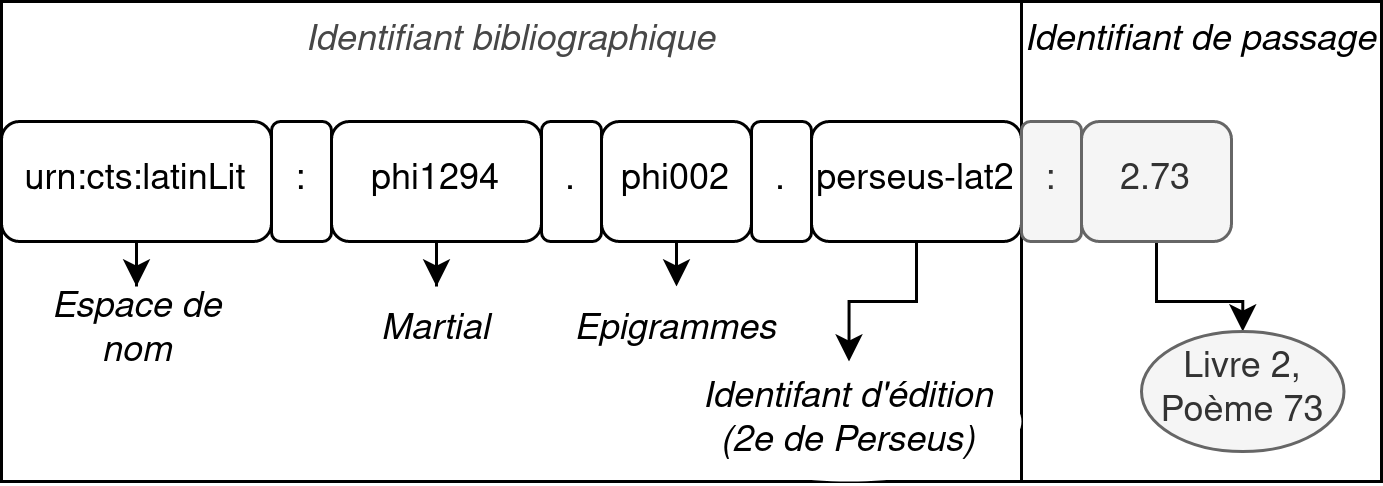
\includegraphics[height=3cm]{figures/chap1/part2/cts-urn.drawio.png}
    \caption{Déconstruction d'un identifiant CTS équivalent au \enquote{Martial, 2, 73}: \texttt{urn:cts:latinLit:phi1294.phi002.perseus-lat2:2.73}}
    \label{fig:chap1:cts_urn}
\end{figure}

% Métadonnées générales (Gillivray ?)
%   -> Reprendre la méthode de datation
% Métadonnées structurelles
%   -> Poser la question de la citabilité et de la section des textes

% Reprendre le travail de Mc Gillivray ici
% La question de la datation
% Poser la question de la citabilité et de la section des textes
% Métadonnées de “lecture”: modèles de citation, niveau de citation recommandé (Introduction du concept de SATU ?)

\subsection{Production et transformations de corpus}

Nous avons défini un cadre théorique à la production de corpus via ses obligations en termes d'éthique scientifique. Il convient désormais de présenter le cadre technique, permettant de réaliser nos objectifs dans les meilleures conditions: obtenir un corpus tel qu'il sera possible d'y retrouver les exemples d'isotopie et d'y faire des recherches lexicographiques. Les conditions de sa production sont donc des conséquences de ces choix: le corpus doit être standardisé et donc en XML-TEI, doit posséder des métadonnées fines, y compris un système d'identification de passages afin de pouvoir revenir à la source ou comparer le texte d'une édition avec une autre. Enfin, il doit avoir une couverture temporelle la plus large possible pour convenir à l'œuvre d'Adams, qui dépasse chronologiquement Isidore\footnote{Le nombre de textes plus tardifs qu'Isidore est très réduit. On ignorera aussi les sources épigraphiques.}. Nous nous intéresserons ici d'abord à la méthode d'encodage et à l'outillage pour produire ce corpus. Ensuite, nous discuterons de sa compilation, à la fois en tant que meta-corpus et en tant que générateurs de versions inédites de textes. Enfin, nous proposerons une analyse des textes contenus, du point de vue des périodes, des quantités et de la diversité d'auteur.


\subsubsection{Choix techniques: XML TEI et Capitains}

La TEI est une \enquote{grammaire}, en cela, elle a l'avantage d'être partagée par de nombreux projets et d'être compréhensible. Mais elle n'est \enquote{que} descriptive: l'exploitation de sa syntaxe ne peut se faire qu'à travers des outils développés pour elle, qu'ils soient faits sur mesure ou partagés par la communauté. Dans ce contexte, nous avons développé depuis 2013 un ensemble d'outils tournés vers l'exploitation et la description des structures logiques de citations et de leurs identifiants. Cet ensemble d'outils, nommé \textit{Capitains}, est constitué de deux pans: un tourné vers l'encodage et l'organisation de corpus, un second cherchant à valoriser, contrôler et exploiter les données ainsi encodées\footcite{clerice_capitains_2015}. Ce cadriciel démarre sous la tutelle des projets Perseus et Perseids et sur la demande de Bridget Almas, ingénieure principale des deux projets\footnote{Officiellement uniquement de Perseids.}, afin de mettre en place un service de distribution de textes qui permette une maintenance rapide et une citabilité pour CTS\footnote{Ce travail est largement décrit, et plus techniquement qu'ici, dans les articles suivant: \textcite{almas_continuous_2018, clerice_les_2017}}. 

Les \textit{guidelines} Capitains identifient dès leur création deux problèmes importantes pour la gestion des corpus de \textit{Perseus}. D'une part, les métadonnées bibliographiques sont particulièrement difficiles à maintenir: chaque fichier du corpus doit contenir des métadonnées sur l'auteur et l'œuvre, quand bien même ces dernières sont multipliées à l'envi, le corpus étant composé d'auteurs prolixes -- comme Cicéron -- et d'œuvres représentées par de multiples éditions et traductions.  D'autre part, les textes doivent être eux-mêmes facilement manipulables et répondre à l'ensemble des besoins de l'API CTS, entre autres ceux de la citabilité et de l'obtention automatique de passages via leur identifiant.

Pour le premier problème, celui de la gestion de corpus et de ses métadonnées bibliographiques, on a procédé à l'extraction de ces dernières en dehors du fichier lui-même. En décrivant les auteurs ou les œuvres hors de celles-ci, la maintenance des informations communes est centralisée et permet de rapidement mettre à jour le catalogue. Pour simplifier encore ce travail, les dépôts \textit{Capitains} doivent suivre une \enquote{syntaxe} pour l'arborescence des fichiers, permettant ainsi de trouver facilement un auteur, ou une œuvre, parmi plusieurs centaines de fichiers. Avec le recul et l'expérience accumulée au fil des années, cette externalisation est à la fois utile -- la compilation du catalogue est extrêmement rapide car elle ne nécessite pas d'ouvrir de gros fichiers TEI -- mais extrêmement inadaptée à de plus petits corpus, qui souffrent d'avantage de la duplication des efforts (métadonnées d'en-têtes TEI, métadonnées de catalogue \textit{Capitains}).

La seconde partie du problème -- plus intéressante pour nous ici -- s'intéresse à la manière de rendre intelligibles à un programme les structures logiques de citations. Grâce à l'explicitation des rôles et des hiérarchies textuelles des noeuds XML, il est possible de produire par exemple des tables des matières pour un logiciel: le fichier devient donc \textit{machine-actionable}. Or, si l'usage de l'expression \enquote{encodage CTS} peut se trouver chez des chercheurs aguerris comme  L.~Muellner\footcite{muellner2019free}, CTS ne déclare aucun moyen de constituer les données et se déclare même \enquote{\textit{technology independant\footcite{smith_brief_nodate}}}: il faut donc trouver une solution technique, pour des sources TEI, à ce problème. Au moment de la production des \textit{guidelines} Capitains, vers 2014, une seule méthode avait retenu notre attention et semblait offrir une solution à ce problème. Nous discuterons ensuite brièvement d'une seconde option, arrivée en 2021 dans les \textit{guidelines TEI}.

CTS définit le texte comme une structure OHCO extrêmement rigide: le texte est un arbre, dont chaque feuille ou branche est un élément citable construisant son propre identifiant à partir de ceux de l'ensemble de ses ancêtres. Ainsi, le numéro de vers d'un poème de Martial ne peut exister qu'avec la référence de son poème et du livre de ce dernier: 2.72.1 est ainsi l'identifiant du premier vers, du soixante-douzième poème du deuxième livre. CTS requiert des identifiants qu'ils soient uniques et les définit comme inséré dans une séquence et une hiérarchie. Les \textit{guidelines} Capitains jusqu'à leur version 2.0 incluse ne peuvent accepter qu'une structure hiérarchique simple, un arbre dont les branches de citation ne peuvent avoir qu'un seul type d'enfant et un seul squelette de chemin XML (appelé xPath): chaque type de passage ne peut être parent que d'un seul type d'enfant, ici livre, poème, vers. Pour décrire cet arbre de citation, les \textit{guidelines} Capitains font appel aux éléments \texttt{cRefPattern} (\textit{Canonical Reference Pattern}) du \texttt{refsDecl} (\textit{References System Declaration}) des \textit{guidelines} TEI. Les niveaux, décrits les uns après les autres, du plus profond au plus proche de la racine, utilisent un système de xPath et d'expressions régulières pour fournir à la machine tout un outillage pour la compréhension des identifiants (1.2.3 est à tel endroit) ou leur reconstitution (1.2.1, 1.2.2, 1.2.3, etc.), comme dans l'exemple \ref{chap1:xml:cRefPattern}.

\begin{figure}[ht]
    \centering
    \lstset{language=XML}
    \begin{lstlisting}[language=XML]
<refsDecl n="CTS">
    <cRefPattern n="line"matchPattern="(\w+).(\w+).(\w+)"
        replacementPattern="#xpath(/tei:TEI/tei:text/tei:body/tei:div/tei:div[@n='$1']/tei:div[@n='$2']/tei:l[@n='$3'])">
    </cRefPattern>
    <cRefPattern n="poem" matchPattern="(\w+).(\w+)"
        replacementPattern="#xpath(/tei:TEI/tei:text/tei:body/tei:div/tei:div[@n='$1']/tei:div[@n='$2'])">
    </cRefPattern>
    <cRefPattern n="book" matchPattern="(\w+)"
        replacementPattern="#xpath(/tei:TEI/tei:text/tei:body/tei:div/tei:div[@n='$1'])">
    </cRefPattern>
</refsDecl>
    \end{lstlisting}
    \caption{\texttt{refsDecl} des \textit{Épigrammes} de Martial dans le dépôt Github de Perseus. Les niveaux sont déclarés du plus profond (les vers) au plus proche de la racine (les livres). Chaque \textsc{replacementPattern} fournit un xPath où les variables \$1, \$2 ou \$3 sont remplacées via le découpage des identifiants autour des points. Le passage 2.72.1 donnera \$1=2, \$2=72, \$3=1 et donc un xPath \texttt{/TEI/text/body/div/div[@n='2']/div[@n='72']/l[@n='1']}}
    \label{chap1:xml:cRefPattern}
\end{figure}

Depuis 2021, une autre option, beaucoup plus élastique et plus simple à l'utilisation pour les encodeurs comme pour les développeurs, a été mise à disposition dans les \textit{guidelines} TEI\footcite{cayless_introducing_2021}. Cette nouvelle méthode de déclaration permet d'échapper non seulement à la complexité des \texttt{cRefPattern} et de clarifier la hiérarchie entre les système de passages, mais aussi d'intégrer des variations bienvenues dans la ridigité de ceux-ci, en autorisant des systèmes différents de citation. Les \texttt{citeStructure} permettent ainsi de générer nom seulement des arbres de citation mais aussi de les qualifier par des métadonnées, avec une complexité technique beaucoup plus faible que celle des premières options susmentionnées (\textit{cf.} \ref{chap1:xml:citeStructure}).

\begin{figure}[ht]
    \centering
    \begin{adjustbox}{width=0.9\textwidth,keepaspectratio}
    \lstset{language=XML}
    \begin{lstlisting}[language=XML]
<refsDecl n="CTS">
  <citeStructure unit="book" match="/TEI/text/body/div" use="@n">
    <citeData property="http://purl.org/dc/terms/title" use="head"/>
    <citeStructure unit="poem" match="div" use="@n" delim=".">
      <citeStructure unit="line" match=".//l" use="@n" delim="."/>
    </citeStructure>
  </citeStructure>
</refsDecl>
    \end{lstlisting}
    \end{adjustbox}
    \caption{Équivalent de la figure \ref{chap1:xml:cRefPattern} utilisant les déclarations \texttt{citeStructure}. Chaque élément repart de la déclaration parente. \texttt{citeData} permet d'ajouter des qualifications (métadonnées) de chaque passage pour la machine.}
    \label{chap1:xml:citeStructure}
\end{figure}

Mais les \textit{guidelines} Capitains ne sont que la première étape, celle de l'explicitation, dans la gestion des structures logiques de citation: elles ne sont qu'une forme de \enquote{sur-TEI}. L'exploitation de ces structures d'encodage est fournie à travers plusieurs outils dont la principale brique est \textit{MyCapytain}, une librairie fournissant un grand nombre de fonctionnalités \enquote{nues} et sans objectif propre à part celle de rendre plus facile le développement autour des \textit{guidelines}. \textit{MyCapytain} permet \enquote{de mettre en action} les informations fournies par les différentes déclarations citées: dans notre cas, elle nous permet de produire une liste des passages extrêmement détaillés, liant chacune des phrases ou des mots à un identifiant complet du type \texttt{urn:cts:latinLit:phi1293.phi002.perseus-lat2:2.72.1} autour d'un code réutilisable et compréhensible. Le corpus peut être ensuite intégralement appelé et chargé à l'aide de ces quelques lignes\footnote{Le traitement du corpus, du téléchargement des nouvelles versions des corpora à leur lemmatisation en passant par leur découpage en segments identifiés par le système d'URN CTS se retrouve dans les notebooks \enquote{Data Preparation - Corpora}. Ce morceau de code est dérivé librement du notebook \enquote{\textit{Step 1}}.}:

\begin{lstlisting}[language=Python]
import glob
from MyCapytain.resolvers.cts.local import CtsCapitainsLocalResolver

repositories = list(glob.glob(CorporaPathList, recursive=False))
resolver = CtsCapitainsLocalResolver(repositories)
for text in resolver.texts:
    if text.lang == "lat":
        # Traitement du texte
\end{lstlisting}

Avec la complexité que représentent l'encodage des structures logiques de citation, leur interprétation dynamique par des logiciels tiers, et les restrictions produites par les recommandations CTS, la constitution de corpus Capitains est plus à même de contenir des erreurs d'encodage que ne sauraient détecter de simples schémas XML. À travers la TEI comme les \textit{guidelines} Capitains, le texte devient un programme: il est donc capable de contenir des bugs, qui sont de l'ordre de la gestion technique de la donnée, à côté de problèmes d'usages, qui relèvent de la gestion qualitative de la donnée. Nous avons donc introduit des outils de contrôle pour cet encodage particulier qui, en testant automatiquement ce dernier, simplifie la validation \enquote{technique} et laisse ainsi le loisir de s'intéresser principalement à la qualité de ce dernier. C'est pourquoi l'ensemble des textes Capitains peuvent être validés par un outil appelé \textit{HookTest}. Cet outil, en plus d'intégrer des tests de schémas TEI, vérifie que chacun des systèmes de déclaration (1) corresponde à des passages uniques, (2) ne croise pas un autre système de citation, (3) ne produise pas de conflit d'identifiants (\textit{cf.} figure \ref{fig:annx:digiliblt-hooktest} en annexe).

\begin{figure}
    \centering
    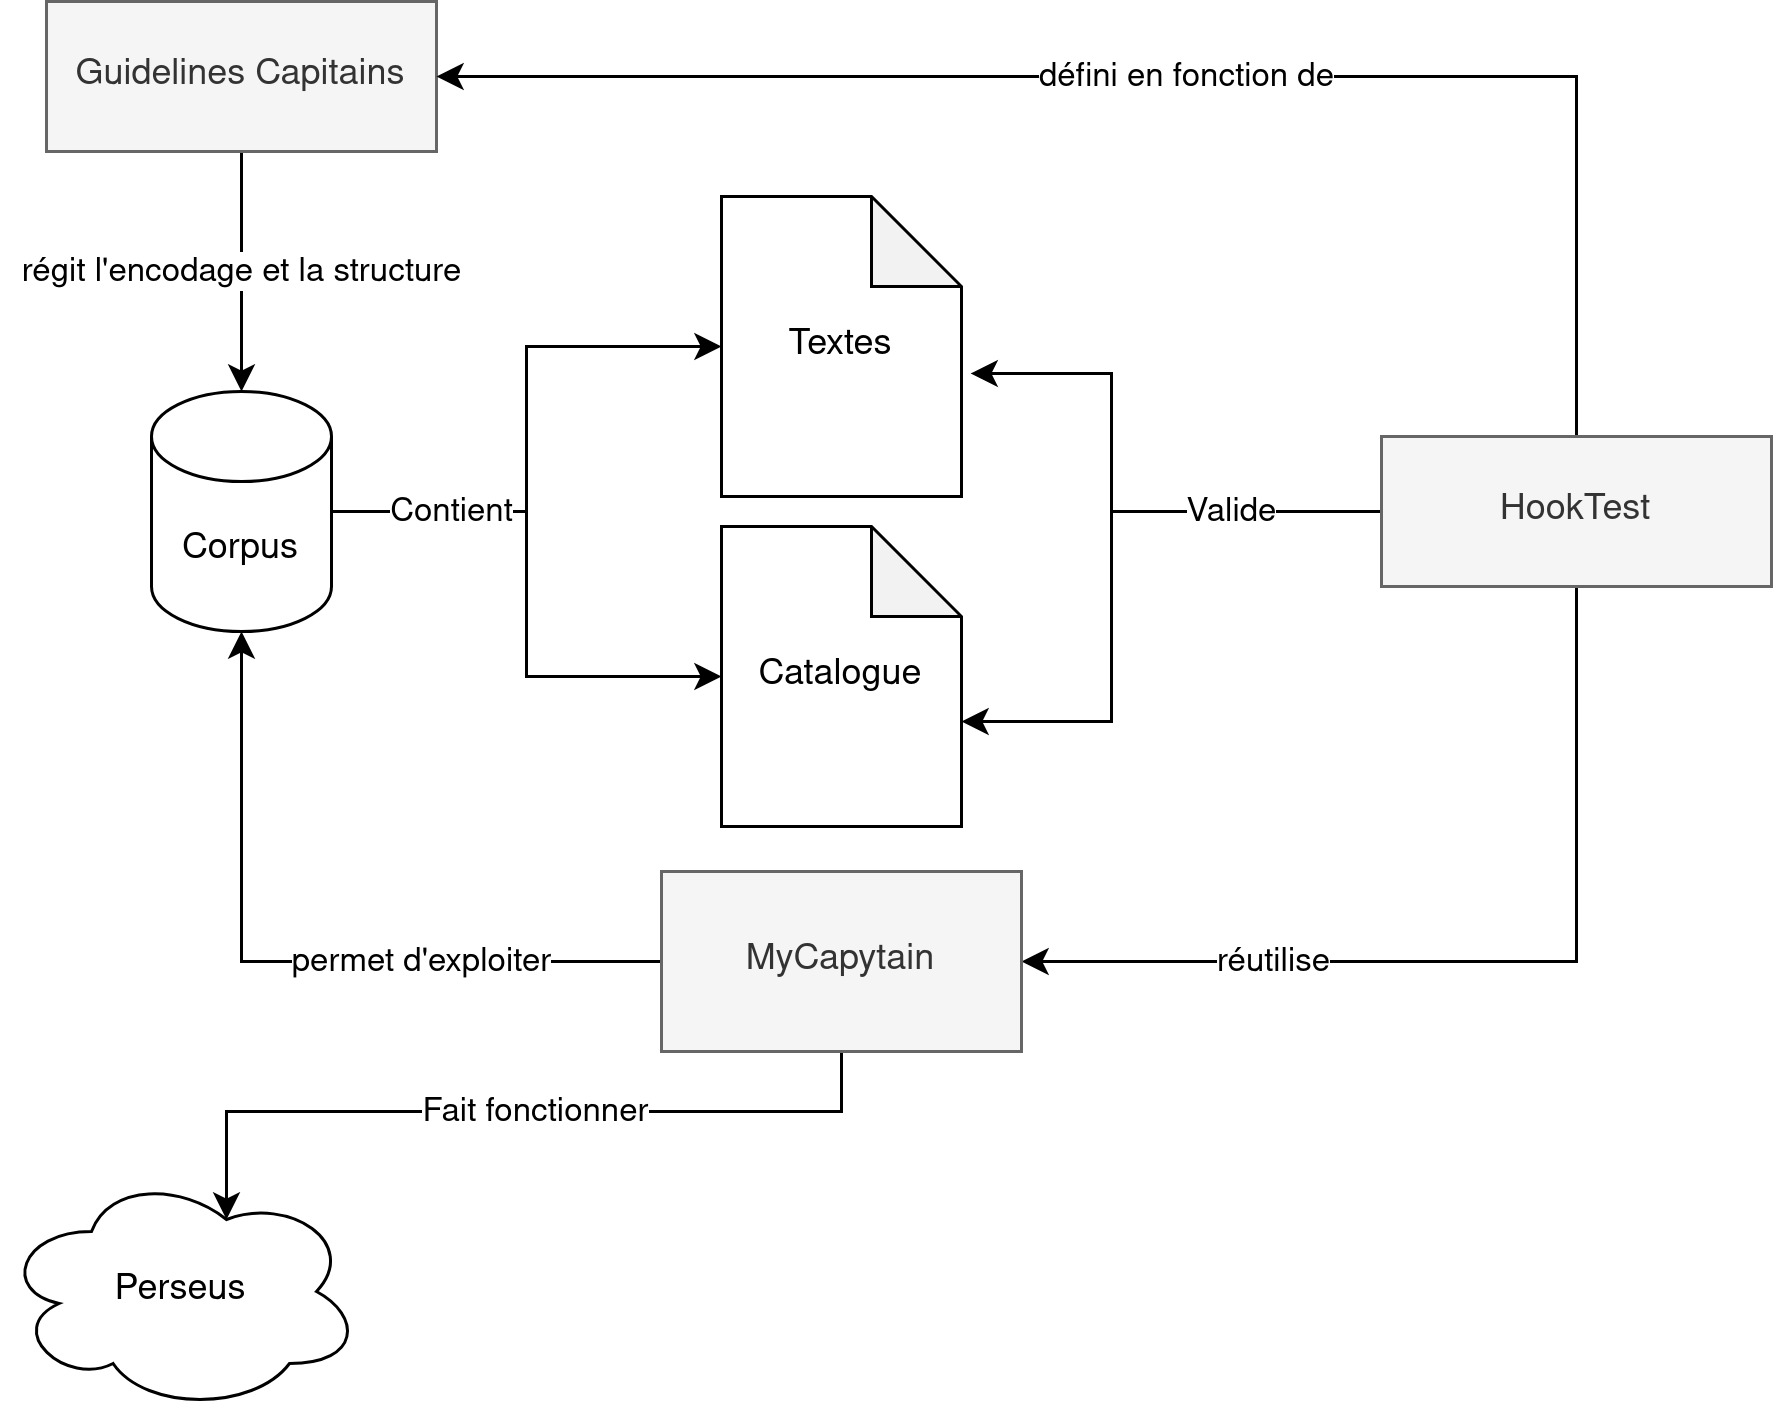
\includegraphics[width=\textwidth]{figures/chap1/part2//capitains.png}
    \caption{Mode de fonctionnement de \textit{Capitains}. \textit{MyCapytain} est une brique commune  l'ensemble des programmes python du monde \textit{Capitains}, elle permet de faire fonctionner autant \textit{HookTest} que \textit{Nautilus}, l'application derrière les serveurs de textes de \textit{Perseus}.}
    \label{fig:chap1:Capitains}
\end{figure}

% Dans la production de corpus, HookTest se situe à la fois comme un outil à utiliser individuellement, pendant la création de fichiers TEI, mais aussi de manière continue dans la vie du corpus. Nos corpus
%Le contrôle qualité des données est un pré-requis important à la construction d'application ou d'analyse. 



\subsubsection{Méthode de compilation, conversion et sources des corpus}

Tous ces choix mènent enfin à la compilation d'un meta-corpus permettant de retrouver et créer notre corpus exemplier. Cette phase de collection et de production est un processus itératif, conditionné à la fois par la mise à disposition de nouvelles sources au format numérique, par la gestion de priorité d'acquisition en fonction de la rencontre d'œuvres chez Adams mais indisponibles dans les corpus au format CapiTainS, et par les opportunités de traitement et d'externalisation de cette mission. Nous discuterons d'abord du travail effectué sur les corpus pré-existants et adaptés à notre cadre technique, puis à l'adaptation de corpus existants.

En effet, l'opportunisme et l'économie d'énergie régissent d'abord notre collecte: nous pouvons commencer par adopter les corpus qui sont déjà adaptés à nos pré-requis techniques. \textit{Capitains} ayant été adopté par la sphère de \textit{Perseus}, et presque uniquement par celle-ci, ce projet et son alter-ego \textit{Open Greek and Latin} sont les premières sources de notre corpus. Pour autant, chacun des corpus disponibles dans ces projets (\textit{Canonical Latin Literature} de \textit{Perseus}, \textit{CSEL} et \textit{PL} d'\textit{OGL}) pose un problème spécifique.

Pour reprendre l'historique de la production de ces corpus et projets, \textit{Perseus} n'avait pas, au début de nos travaux de recherche, converti l'ensemble de ses textes aux \textit{guidelines Capitains}, encore moins pour ses textes latins. De 2013 à 2016, l'ensemble des conversions de textes latins des dépôts Perseus datant d'avant l'obtention de la chaire à Leipzig avait été réalisé par nos soins, sans que cela soit une mission prioritaire du laboratoire. La majeure partie des efforts de l'équipe se concentre d'abord sur les textes du CSEL puis sur les textes de la PL. En avril 2017, au moment de notre départ de Leipzig, le corpus ne contenait que 390 textes convertis sur 674, traductions incluses, pour un total d'environ 5,07 millions de mots en latin\footcite{travis_hook_2017, travis_hook_2017_logs}. En décembre 2021, ce total est monté à 418 textes sur 686, avec une augmentation de plus d'un million de mots\footnote{6~159~948 mots latins pour êtres précis, d'après \textcite{travis_hook_2021_logs}}. L'une des sources principale de cette augmentation est la conversion de l'ensemble du corpus de Cicéron, produite dans le cadre de notre méta-corpus. Ces modifications des données de \textit{Perseus}, aussi justes soient elles, ont besoin d'être validées par l'équipe actuelle du projet et donc de rentrer dans le calendrier de production des données de Perseus. Sur ce dernier point, on notera qu'en décembre 2021 deux conversions effectuées pour le méta-corpus\footcite{noauthor_pull_nodate} étaient encore en attente de validation par l'équipe actuelle du projet: elles ne rentraient pas dans le calendrier de rétro-conversion des sources, principalement tourné vers le grec et les traductions\footnote{Il n'est en aucun cas question ici de jeter la pierre sur d'anciens collègues, mais de mettre en avant les problèmes que peuvent poser parfois ce genre de collaboration, à travers l'existence de priorités, d'attentes et de missions différentes.}. 

Un cas particulier de conversion pour le corpus principal de \textit{Perseus}, \textit{Canonical Latin Literature}, est celle des \textit{Annales} de Tacite. Ce texte -- dont \textit{Perseus} possédait plusieurs éditions -- a été victime d'un problème de conversion entre les diverses versions de la plate-forme qui a donné lieu à la segmentation involontaire de plusieurs éditions du texte en quarante-sept œuvres sans distinction des regroupement originaux\footcite{noauthor_canonical_latinlitphi0660phi003perseus_lat2xml_nodate, clerice_phi0914phi001lat2_nodate}. Sa \textit{capitainisation} est impossible à partir des fichiers \textit{open source} trouvables dans les dépôts du projet, car elle demande alors une connaissance de l'historique des migrations pour en déduire l'origine des problèmes et un travail minutieux de transformation d'une TEI P4 vers une TEI P5 Capitains. C'est à travers une collaboration entre d'anciens employés et des employés actuels que cette conversion a été rendue possible.

Outre le corpus original \textit{Canonical Latin Literature}, Perseus et le projet \textit{Open Greek and Latin} ont mis à disposition deux autres corpus: le CSEL et la PL. Ces deux derniers ont la particularité d'être des corpus extrêmement récents dans l'histoire de Perseus, produits majoritairement via OCR et dont la structuration en XML TEI a été externalisée à une entreprise n'étant pas composée de latinistes ou d'hellénistes mais d'encodeurs de documents administratifs. Cette méthode de production de données a engendré deux grands problèmes. D'une part, l'OCR peut présenter des erreurs, anodines souvent, particulièrement problématiques pour notre étude parfois. On notera par exemple l'erreur répétée de segmentation d'\textit{oraculum} en deux mots (\textit{ora} et \textit{culum}, de \textit{culus}) suite à la non résolution d'une hyphénation qui n'avait plus lieu d'être dans le document XML, mais aussi de \textit{sae-culum}, d'\textit{o-culus}, de \textit{claui-culus}, \textit{taberna-culum}, etc\footnote{Quelle ne fut pas notre surprise quand nous trouvions, par moteur de recherche, un grand nombre d'emplois de \textsc{culus} chez Augustin d'Hippone.}. D'autre part, l'encodage des structures logiques de citation a pu poser des problèmes, car sa formalisation typographique peut fluctuer d'une impression à l'autre, d'autant plus sur des périodes de productions comme celle de la CSEL (plus d'un siècle), et il peut être difficile de faire la différence entre un numéro de ligne, un numéro de section, etc. Cette reproduction de l'information demande alors à la fois une compréhension des mécanismes d'édition et de langues, afin de séparer les identifiants de section du texte: il ne s'agit pas seulement de reconnaître les sauts de lignes qui sont des vers ou des changements de paragraphes, mais aussi le rôle du paratexte qui les accompagne.

La constitution de ces corpus a aussi eu le malheur d'avoir lieu pendant la formalisation des \textit{guidelines} Capitains. Il a donc fallu, après la réception des données, non seulement reprendre les structures logiques mais aussi intégrer les informations requises pour leur exploitation. Ce travail a été achevé pour la CSEL au cours de l'année 2017 par Matt Munson, employé de Leipzig à cette époque, mais pas pour la PL, la laissant \enquote{en friche} du point de vue de sa compatibilité avec les outils de l'écosystème \textit{Perseus}. Cet abandon du corpus, au moins momentané, est un exemple supplémentaire du changement politique et économique de la production de corpus de \textit{Perseus}. Le projet \textit{First Thousand Years of Greek} du CHS apporte plus de fonds, les textes de la patrologie latine sont disponibles par ailleurs sur d'autres plates-formes: le projet change de priorités de production de corpus. Un seul corpus supplémentaire est né depuis 2017 en latin: le corpus OGL/Latin. Il contenait deux textes au moment de la compilation du meta-corpus.

CSEL et canonical-latinLit mis ensemble, le corpus représente environ douze millions de mots, dont les épicentres thématiques et chronologiques sont respectivement les pères de l'Église de l'antiquité tardive et la littérature classique de la Rome pré-chrétienne. Il reste alors pour couvrir les périodes présentes chez Adams, en plus de quelques textes non convertis chez \textit{Perseus}, trois pans:

\begin{enumerate}
    \item l'épigraphie. Elle est intégralement ignorée dans notre corpus pour des raisons évoquées plus tôt, comme le problème important de sa lemmatisation.
    \item la période tardive non-chrétienne, en particulier les littératures médicales (importants pour notre recherche) et celles des grammairiens.
    \item la littérature de la période classique peu connue ou peu étudiée avant le niveau master en lettres classiques: \textit{Perseus} se concentre d'abord historiquement sur les corpus les plus communs pour rendre leur accès plus facile. 
\end{enumerate}

Pour le deuxième comme pour le troisième pan, la règle principale pour l'intégration de textes au meta-corpus a été leur mention par Adams dans son ouvrage: tout texte dans les bornes chronologiques mentionnées -- c'est-à-dire avant la mort d'Isidore de Séville -- a fait l'objet d'une recherche quant à la disponibilité d'une édition numérique correspondante dans un corpus tiers. Dans le cas où le code pour la conversion d'une édition XML-TEI, HTML ou plein texte était facilement réutilisable pour convertir d'autres œuvres similaires d'un même site, nous ajoutions à l'œuvre mentionnée par Adams les œuvres similaires convertissables à bas coût. Ces conversions ont été mises à disposition dans deux corpus distincts: pour les œuvres du projet \textit{DigilibLT}, projet encore actif et centré sur un des angles morts des corpus Perseus, la littérature tardive non chrétienne, un corpus miroir \textit{DigilibLT-Capitains}\footcite{Clerice_Digital_Latin_Library_2021} a été mis en développement par nos soins; pour les autres œuvres, issues de sources diverses (\textit{cf.} table \ref{tab:chap1:corpusutilises}), un corpus sobrement nommé \enquote{\textit{Lasciva Roma - Additionnal Texts}}\footcite{Clerice_Corpora_of_rare_2021} a vu le jour. Le premier compte 103 textes\footnote{sur 216 téléchargés de \textit{DigilibLT}} et 2,8 millions de mots, le second 134 textes et 3,8 millions.


\begin{table}[h]
    \centering
    \begin{tabular}{lr}
        \toprule
        Corpus numérique ou édition numérique utilisée & Fréquence \\
        \midrule
         OBI\footnotemark            & 73 \\
         Lacus Curtius\footnotemark         & 18 \\
         Corpus Corporum\footnotemark & 12 \\
         Horatius.net\footnotemark    & 12 \\
         The Latin Library\footnotemark   &  4 \\
         Musisque Deoque\footnotemark &  3 \\
         Perseus        &  3 \\
         Remacle\footnotemark        &  2 \\
         ALIM\footnotemark           &  1 \\
         Lesley Bolton\footnotemark         &  1 \\
         Latin Law Library\footnotemark    &  1 \\
         Monumenta Germanica Historica\footnotemark            &  1 \\
         Corpus Scriptorum Latinorum\footnotemark            &  1 \\ \midrule
         Éditions originales à partir d'OCR    &  2 \\
        \bottomrule
    \end{tabular}
    \caption{Source des corpus utilisés. Deux sortent du lot. OBI présente 73 éditions, un nombre surgonflé: il y a 73 livres pour la \textit{Vulgate} d'après CTS). Nous remercions chaleureusement Lesley Bolton, docteure canadienne, de nous avoir permis de réutiliser son travail de thèse pour en faire une édition TEI. Les éditions originales à partir d'OCR ont été produites à partir des données d'\textit{Internet Archive}.}
    \label{tab:chap1:corpusutilises}
\end{table}
\footnotetext{\textcite{barry_schein_open_1994}.}
\footnotetext{\textcite{lomarcan_lacuscurtius_1999}.}
\footnotetext{\textcite{roelli2014corpus}}
\footnotetext{\textcite{horatiusnet}.}
\footnotetext{\textcite{carey_latin_1998}}
\footnotetext{\textcite{gelderblom_musisque_2008}.}
\footnotetext{\textcite{philippe_remacle_site_2008}.}
\footnotetext{\textcite{d2019alim}.}
\footnotetext{\textcite{bolton_edition_2015}.}
\footnotetext{\textcite{lassard_roman_2001}.}
\footnotetext{\textcite{noauthor_openmgh_nodate}.}
\footnotetext{\textcite{csl}.}

Pour le troisième point, un texte fondamental pour notre recherche est absent des corpus Perseus: les \textit{Priapées}\footcite{Clerice_Digital_edition_of_2020}. Il s'agit d'un ensemble de poèmes plutôt courts et centrés autour de la personnalité de Priape, dieu gardien des vergers dont l'arme principale est un sexe en érection. Il est constitué de deux blocs, une partie de ses poèmes y ayant été ajouté par analogie au cours des éditions du texte\footcite{callebat_les_2008}. Pour la mettre à disposition, nous avons réutilisé le texte et les traductions de R. F. Burton et L. C. Smithers de 1890\footcite{burton_priapeia_1890} comme première version du texte. Cette base de texte nous a évité de passer par la fastidieuse case de l'OCR, de sa correction et de la qualification de ses lignes en vers, poèmes ou notes de bas de page. Nous l'avons ensuite adapté en fonction de l'édition scientifique d'Emil Baehrens parue chez Teubner\footcite{baehrens_poetae_1910}. Ce texte a été intégralement traduit pour la présente recherche et annoté linguistiquement en lemme et en morpho-syntaxe: cette phase d'annotation a permis de relire intégralement le texte, et de le comparer avec l'édition de Louis Callebat paru en 2012 aux Belles lettres et dont nous avons utilisé la réimpression de 2017\footcite{callebat_priapees_2012}. Si les variations entre les deux éditions sont faibles, on a préféré donner en apparat critique quelques choix de l'éditeur français quand elles respectaient l'intégralité des manuscrits là où l'éditeur allemand en produisait une minoritaire. Comme la majeure partie des éditions de Perseus, cette édition numérique des Priapées a plus pour vocation de donner un texte qu'une édition critique, hormis ces quelques notes importées de la comparaison avec l'édition la plus récente.

\begin{figure}
    \centering
    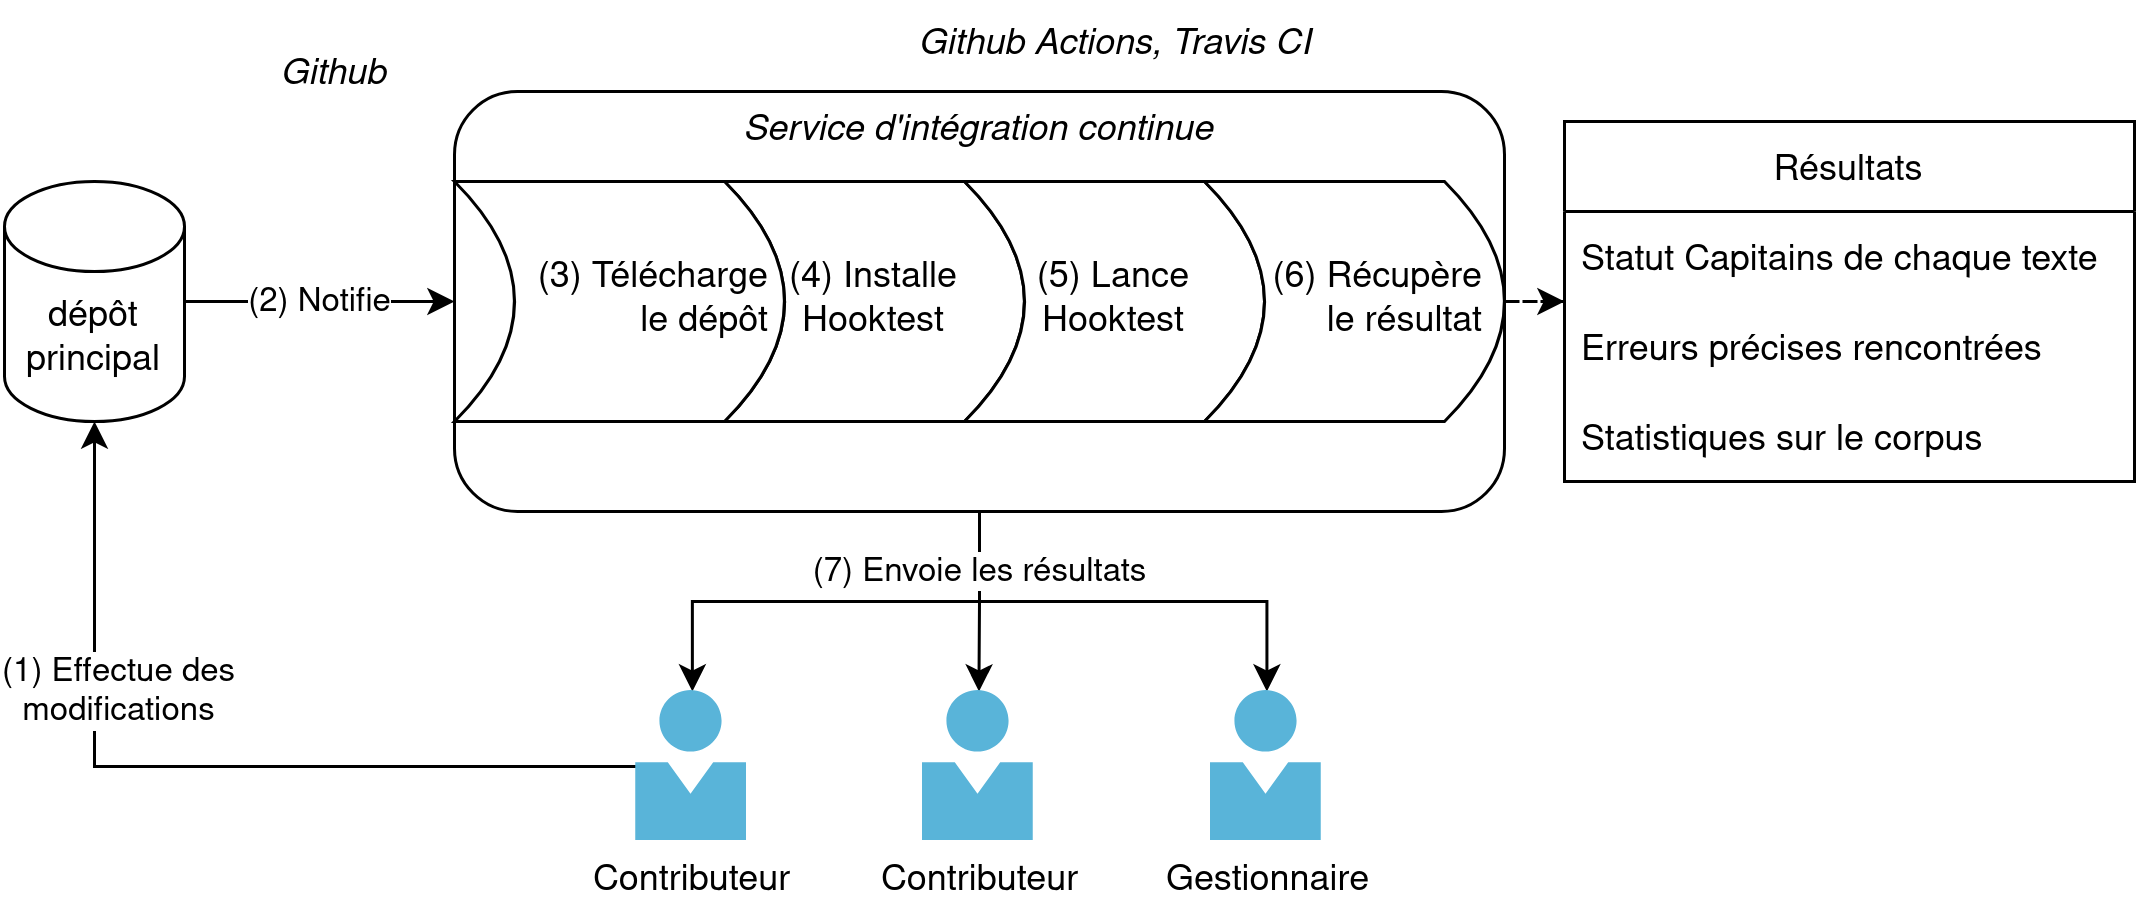
\includegraphics[width=\linewidth]{figures/chap1/part2/hooktest.png}
    \caption{Processus automatisé}
    \label{fig:chap1:ci}
\end{figure}

Une partie du travail sur \textit{DigilibLT-Capitains} et la majeure partie de la conversion de Tacite ont été réalisées dans le cadre de devoirs fournis aux étudiants et étudiantes des master \enquote{Technologies Numériques Appliquées à l'Histoire} (TNAH) et \enquote{Humanités Numériques} de l'ENC et de PSL. Dans le cadre de l'apprentissage des outils de versionnage Git, cinquante-six éditions du projet italien ont été \enquote{capitainisées}, les textes retenus ayant été choisis librement par les étudiants. Cet exercice permettait à la fois de comprendre les enjeux de la collaboration sur plate-forme numérique, avec une dizaine de collaborateurs travaillant sur des données partagées, ses bonnes pratiques et la gestion des contrôles qualités. En effet, \textit{HookTest} permet aussi d'être utilisé comme un outil de contrôle automatique des corpus sur des plate-forme comme Github dans le cadre d'intégration continue, c'est-à-dire dans le cadre de tests automatisés et décentralisés lancés à chaque modification du dépôt contenant les données (\textit{cf.} figure \ref{fig:chap1:ci}).
% Ces corrections demandent à la fois une compréhension de la langue et des règles de mise en page. 
% Description des corpus ciblés et du processus itératif d'adaption du corpus

% Enfin, statistiques sur le corpus.
    % Statistiques sur les corpus Perseus et autres
    % La conversion de DigilibLT
    % Présentation des corpus Lasciva Roma
    %% Priapées
    %% Additional-Texts
    
\subsubsection{Description du meta-corpus final}

Le meta-corpus final est formé des six corpus \textit{open-source} et libres de droit mentionnés pour un total d'une vingtaine de millions de mots (\textit{cf.} table \ref{tab:chap1:corpora}). Il est constitué de 204 auteurs ou regroupements d'œuvres (par exemple, le \textit{Nouveau Testament} compte comme un regroupement de textes) pour 853 œuvres. Tous les textes cités par le TLL ou par Adams n'ont pas pu être ajoutés au corpus: on note par exemple l'absence des \textit{Declamationes minores} de Quintilien, des commentaires de Donat ou de textes du \textit{Corpus Grammaticorum Latinorum}. Nous avons suivi les principes de production de corpus originaux de Perseus, à savoir de ne pas inclure les auteurs fragmentaires: majoritairement collectés via des citations chez d'autres auteurs, leur introduction pourrait introduire du bruit. 

En dehors des manques particuliers à la collecte ou à l'histoire des corpus réutilisés, notre corpus présente des caractéristiques assez attendues d'un corpus de sources anciennes et littéraires. Il est constitué majoritairement d'auteurs dont on ne possède qu'une seule œuvre (près de 120 auteurs sont dans ce cas) avec quelques auteurs extrêmement prolifiques, comme Augustin et Cicéron avec une soixantaine d'œuvres (\textit{cf.} \ref{fig:chap1:œuvres-par-auteur}). Les textes sont assez courts: les trois quarts font moins de 20~000 mots (\textit{cf.} table \ref{tab:chap1:mots-par-textes}). Quatre-vingts textes font moins de mille mots (10\% du corpus) tandis que quarante neuf en font plus de cent mille. Les textes les plus grands atteignent le million de mots (\textit{cf.} \ref{fig:chap1:mots-par-texte}).

Chaque corpus du meta-corpus concerne une période qui lui est propre (\textit{cf.} figure \ref{fig:chap1:mots-par-corpus}): \textit{Canonical Latin Literature} de \textit{Perseus} propose des œuvres majoritairement issues de la période classique, de -254 à 150 de notre ère. Il connaît une légère production supplémentaire aux alentours du IVe siècle avec les œuvres de Jérôme et d'Ausone, incluses par l'équipe du projet pour des raisons pédagogiques. Le deuxième grand corpus, le CSEL, couvre la période de 300 à 950 avec les pères de l'Église. Le corpus \textit{DigilibLT} est constitué d'œuvres écrites principalement entre la fin du IIIe siècle au Ve. Au contraire des autres corpus, \textit{Additional Texts} ne présente pas d'homogénéité dans sa production: il est le fruit d'un \enquote{remplissage des manques} et génère donc des inégalités de tailles en fonction des périodes. Il connaît deux pics importants: le premier est formé de la rédaction de la \textit{Vulgate} et des commentaires de Servius pendant le IVe siècle; au Ve siècle, le second pic est constitué d'un seul texte massif, le \textit{Code Justinien}.

\afterpage{%
\begin{table}
\begin{minipage}{.4\linewidth}%
        \centering
        \resizebox{\textwidth}{!}{%
        \begin{tabular}{lr}%
            \toprule
            Corpus                         & Version \\ \midrule
            PerseusDL/canonical-latinLit & 0.0.843 \\
            OpenGreekAndLatin/csel-dev   & 1.0.223 \\
            lascivaroma/priapeia         & 1.1.18  \\
            lascivaroma/additional-texts & 1.0.193 \\
            lascivaroma/digiliblt        & 0.0.64  \\
            OpenGreekAndLatin/Latin      & v1.11.0 \\ \bottomrule
        \end{tabular}%
        }
        \caption{Corpus utilisés pour la formation du meta-corpus de sources.}
        \label{tab:chap1:corpora}
\end{minipage}%
\hfill
\begin{minipage}{.56\linewidth}%
        \centering
        \resizebox{\textwidth}{!}{%
        \begin{tabular}{l|rr|rr}
            \toprule
                      Auteur &      Mots &  Rang      &  œuvres &  Rang         \\
            \midrule
                    Augustin & 2~566~421 &          1 &       68 &             2 \\
                   Justinien & 1~430~321 &          2 &        2 &            62 \\
                     Cicéron & 1~389~163 &          3 &       60 &             3 \\
                      Jérôme &   879~855 &          4 &        9 &            19 \\
                     Servius &   717~622 &          5 &        4 &            34 \\
                    Ambroise &   685~483 &          6 &       19 &            10 \\
                  Tertullien &   678~635 &          7 &       50 &             4 \\
                   Tite-Live &   614~940 &          8 &        1 &            87 \\
                     Vulgate &   603~091 &          9 &       73 &             1 \\
                     Sénèque &   525~489 &         10 &       27 &             7 \\ 
                            \multicolumn{5}{c}{...}                \\
                      Plaute &   233~258 &         23 &       20 &             9 \\
            Histoire Auguste &   128~128 &         35 &       30 &             5 \\
                      Ausone &    68~418 &         67 &       29 &             6 \\
              Cornelius Népos &    33~604 &         89 &       25 &             8 \\
            \bottomrule
        \end{tabular}%
        }
        \caption{Auteurs ou groupes de textes les plus importants en œuvres et en mots, classés par le nombre de mots.}
        \label{tab:chap1:rang-auteurs}
\end{minipage}
\end{table}
\begin{figure}
    \centering
    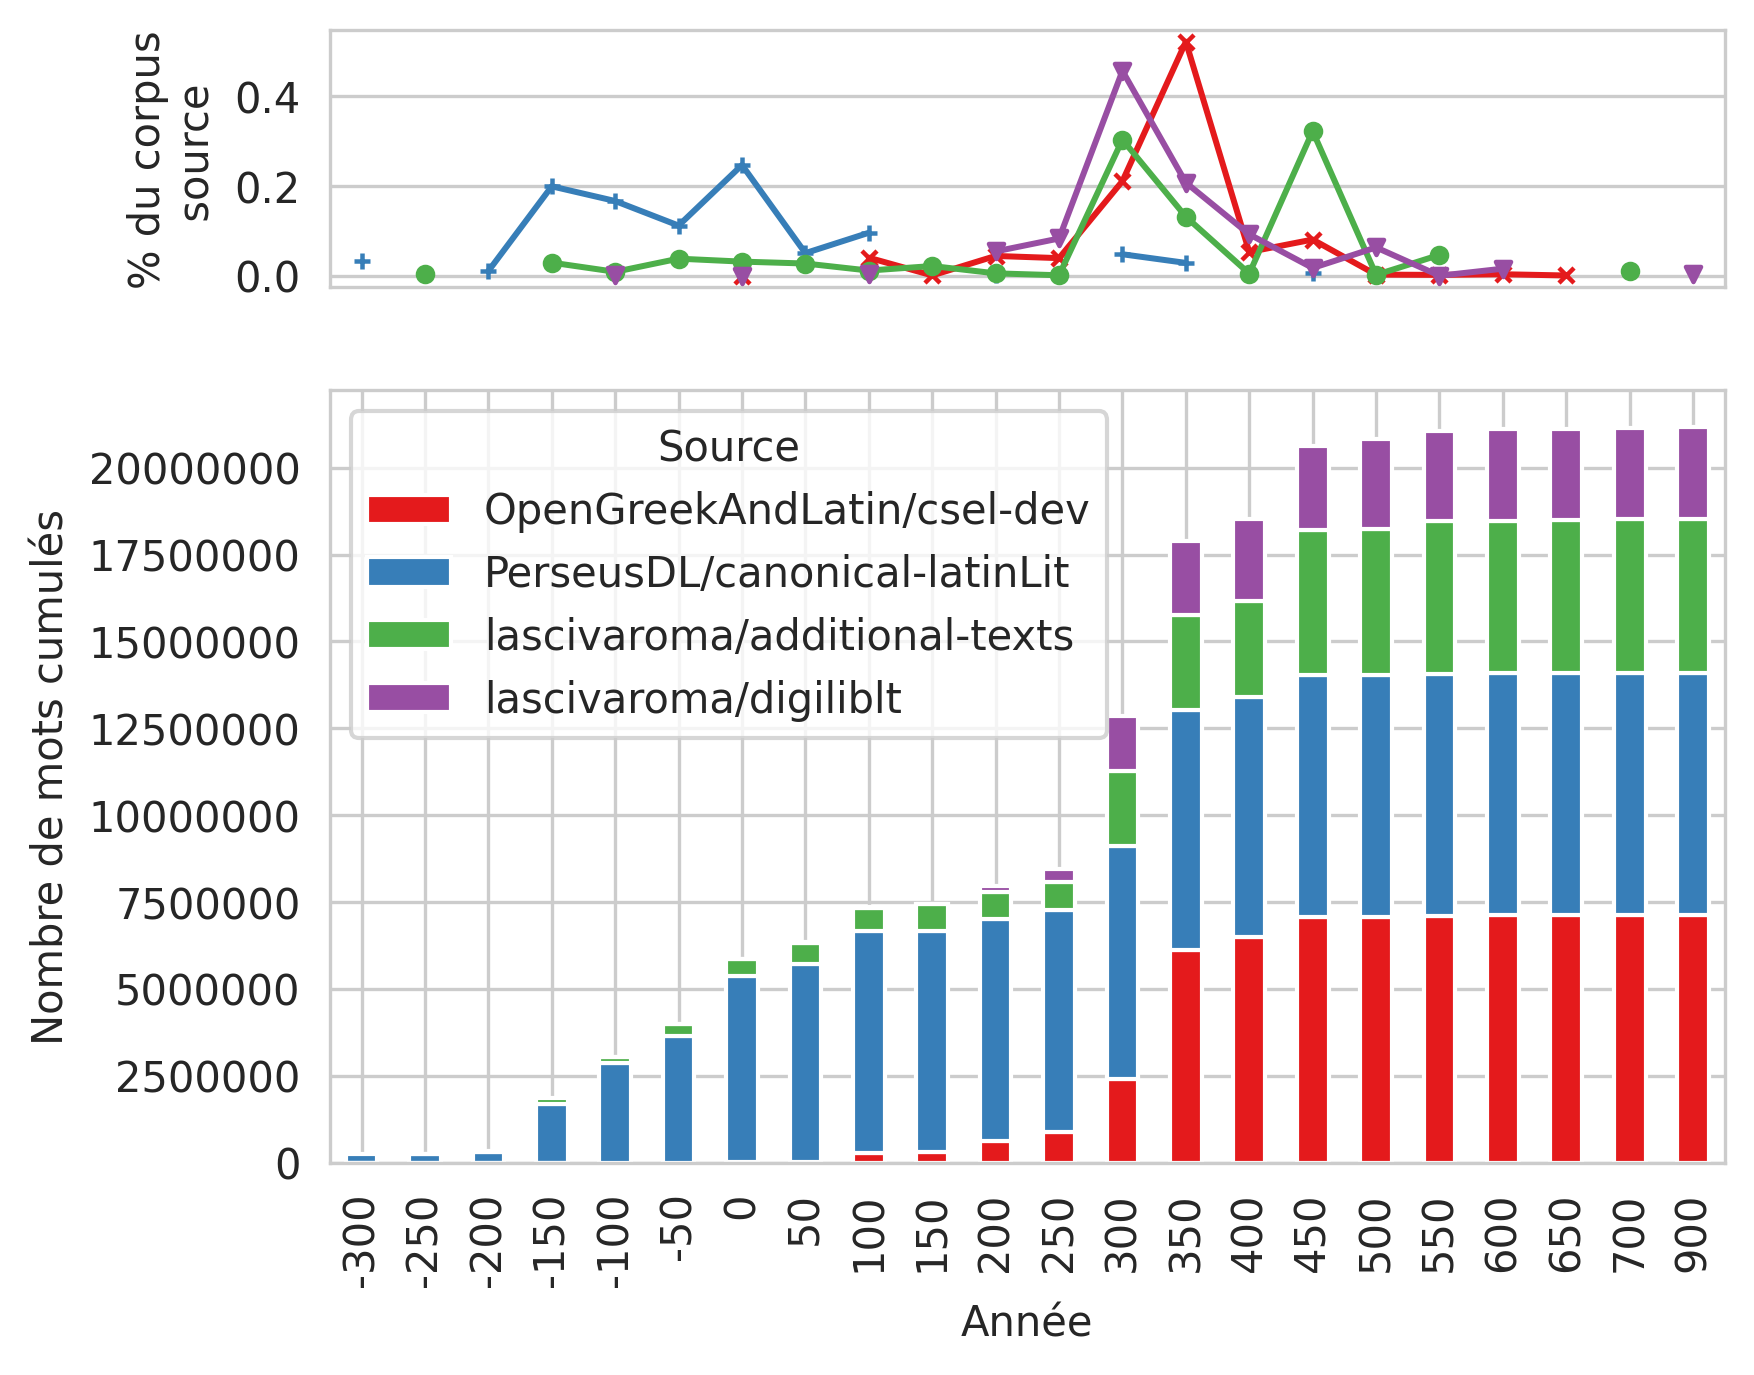
\includegraphics[width=.9\linewidth]{figures/chap1/part2/motsPaCorpus.png}
    \caption{Évolution de la taille du meta-corpus par corpus et par demi-siècle. La partie supérieure du graphe présente les pourcentages relatifs à chaque corpus, la partie inférieure les valeurs absolues en nombre de mots.}
    \label{fig:chap1:mots-par-corpus}
\end{figure}
\clearpage
}

Le meta-corpus contient par ailleurs deux grandes périodes de rédaction, correspondant à deux phénomènes bien identifiés par les historiens de la littérature (\textit{cf.} \ref{fig:chap1:accum-mot}). On a d'une part la littérature dite classique, allant de la fin de la République au règne des Antonins à la fin du Ier siècle de notre ère: elle est constituée -- entre autres -- du graphomane Cicéron, des philosophes Sénèque et Lucrèce, des poètes augustéens et de l'apogée du genre élégiaque, des épopées latines les plus connues, et se termine avec les écrivains Martial, Juvénal et Pline le Jeune. Ces siècles ont été consacrés par l'enseignement du latin à travers le thème, dont la langue est calquée sur les styles césariens et cicéroniens, et l'études des grands classiques comme l'\textit{Énéide} de Virgile et les \textit{Annales} de Tacite\footnote{Il suffit de voir que l'\textit{Anthologie de la littérature latine} de J. Gaillard et R. Martin s'arrête à Apulée (IIe siècle) et ignore l'ensemble de la littérature chrétienne et tardive pour se rendre compte de la focalisation de la réception sur cette période de la littérature. \textcite{gaillard_anthologie_2005}}. Cette période représente un peu moins de la moitié du corpus avec près de dix millions de mots. 

La deuxième période de production massive est ce que Fredouille et Zehnacker appellent \enquote{l'âge d'or de la patristique}\footcite{zehnacker_litterature_2013}: avec la reconnaissance officielle du christianisme, on assiste à la rédaction des œuvres d'Hilaire, Ambroise, Augustin et de Jérôme, dont la production -- partiellement représentée dans notre corpus -- correspond à 20,7\% du meta-corpus complet en nombre de mots et 12,5\% en nombre de textes. D'autres auteurs, aux quantités minuscules par rapport à celles des quatre Pères, restent majeurs pour notre recherche: ainsi, le IVe siècle est aussi le siècle d'Ausone, et donc du \textit{Centon Nuptial}, ré-arrangement littéraire des vers de Virgile visant à raconter un mariage et la première nuit des mariés. C'est aussi le siècle des grammairiens et des commentaires: on y retrouve l'œuvre de Donat, de Servius et, suivant les datations, des \textit{Adnotationes super Lucanum}. Les commentaires peuvent avoir une grande importance pour la compréhension des textes anciens ou du moins de leur réception, et, en termes d'approche quantitative, permettent d'ajouter du contexte aux passages originaux.

Pour ce qui est des manques, ils peuvent être particulièrement compliqués à quantifier. Si l'on en croit le nombre de textes convertis du DigilibLT, il y aurait au moins autant de textes tardifs hors-patristique absents que présents de notre corpus. Pour la patristique, le \textit{Corpus Corporum} fournit une taille pour chaque corpus: la patrologie latine serait formée de quatre-vingt huit millions de mots. Ce chiffre doit être pris comme un ordre de grandeur, car les documents XML de la PL du projets fourmillent de citations en plein texte du type \enquote{(Joan. XV, 17).}, représentant un bruit important pour le décompte de mots. Il reste qu'avec ce nombre, plus de quatre fois la taille de notre corpus, il est certain que nous avons des manques: Jérôme y est représenté par 2,5 millions de mots pour 105 œuvres (en ne comptant que les œuvres attribuées assurément par le projet), tandis que le méta-corpus culmine à 880~000 mots pour 9 œuvres (\textit{cf.} \ref{tab:chap1:rang-auteurs}). La conversion et la collecte des textes ayant été guidées par les citations du TLL et d'Adams, ces auteurs sont sous-représentés.


Pour la période classique, nous bénéficions du travail du \textit{Perseus Catalog}\footcite{babeu2019perseus} et du PHI. Projet enfant de \textit{Perseus}, le catalogue, dirigé par Alison Babeu, a pour vocation de répertorier les auteurs, œuvres, éditions et traductions des auteurs antiques, et tout particulièrement celles tombées dans le domaine public. Ce catalogage s'accompagne souvent de liens vers des textes disponibles sous formes de numérisations PDF sur les plates-formes comme \textit{Google Book}, \textit{Internet Archive} ou \textit{Hathi Trust}. Il est complété du nombre de mots quand l'œuvre est disponible sur le PHI. Ce décompte, visible en figure \ref{fig:chap1:accum-mot-diff-perseus-catalog}, permet d'estimer qu'il manque -- au plus -- quelques centaines de milliers de mots sur la période classique. Mais tout comme les chiffres de la PL, il est à interpréter avec précaution: en étudiant les auteurs dont les œuvres sont sous-représentées (\textit{cf.} figure \ref{fig:chap1:ecarts-auteurs}), nous avons trouvé qu'Ovide aurait près de deux cent mille mots de moins dans notre meta-corpus que chez le PHI. Or, Ovide n'est pas l'auteur d'un très grand nombre d'œuvres ou de recueil, et un tel manque ne pourrait être que la trace de l'oubli d'un classique par \textit{Perseus} dont le projet même était de mettre à disposition les textes couramment étudiés. En cherchant les données manquantes, il s'est avéré que le texte incriminé est une œuvre mineure, \textit{l'Epicedion Drusi}, un poème de 474 vers dont le nombre de mots est évalué à tort à plus de deux cent vingt mille mots par le catalogue\footcite{clerice_catalog_dataphi0959phi015_2021}. L'écart qui sépare notre meta-corpus du corpus du PHI pourrait donc être moindre que ce qui est affiché par le \textit{Perseus Catalog}. Il reste probable que Cicéron (dont les œuvres complètes ne sont pas toutes présentes sur Perseus), Sénèque (dont quelques ouvrages manquent) et Quintilien (dont il nous manque au moins les \textit{Declamationes Minores}) soient véritablement parcellaires dans le meta-corpus.

Pour conclure, nous faisons face à un meta-corpus varié dont le caractère incomplet est dû en partie aux critères initiaux, à savoir la possibilité d'exploiter mécaniquement les ressources textuelles via une explicitation de leurs structures. S'il devait être complété, les tâches suivantes devraient être réalisées en priorité:
\begin{itemize}
    \item la conversion complète des œuvres du \textit{DigilibLT};
    \item la conversion des textes de la patrologie latines dont les auteurs précèdent ou sont contemporains d'Isidore de Séville;
    \item la conversion et l'obtention des textes des grammairiens latins, dont le corpus n'a pas pu être obtenu à temps, soit à travers le \textit{Corpus Grammaticorum Latinorum}, dont les sources sont réutilisées par le C\textit{orpus Corporum}, soit à travers le projet \textit{HyperDonat};
    \item la création d'éditions \enquote{fac-similaires} simples, à la \textit{Perseus}, pour les textes des auteurs classiques manquants, au premier titre desquels figurent Cicéron et Quintilien.
\end{itemize}
Ces recommandations sont par ailleurs dépendantes de l'évolution des techniques de lemmatisation, dont l'adaptation aux textes documentaires et épigraphiques nous pousserait à recommander d'incorporer, surtout pour notre thématique, les inscriptions et graffitis, dont ceux de Pompei.


\afterpage{%
\begin{figure}
    \centering
    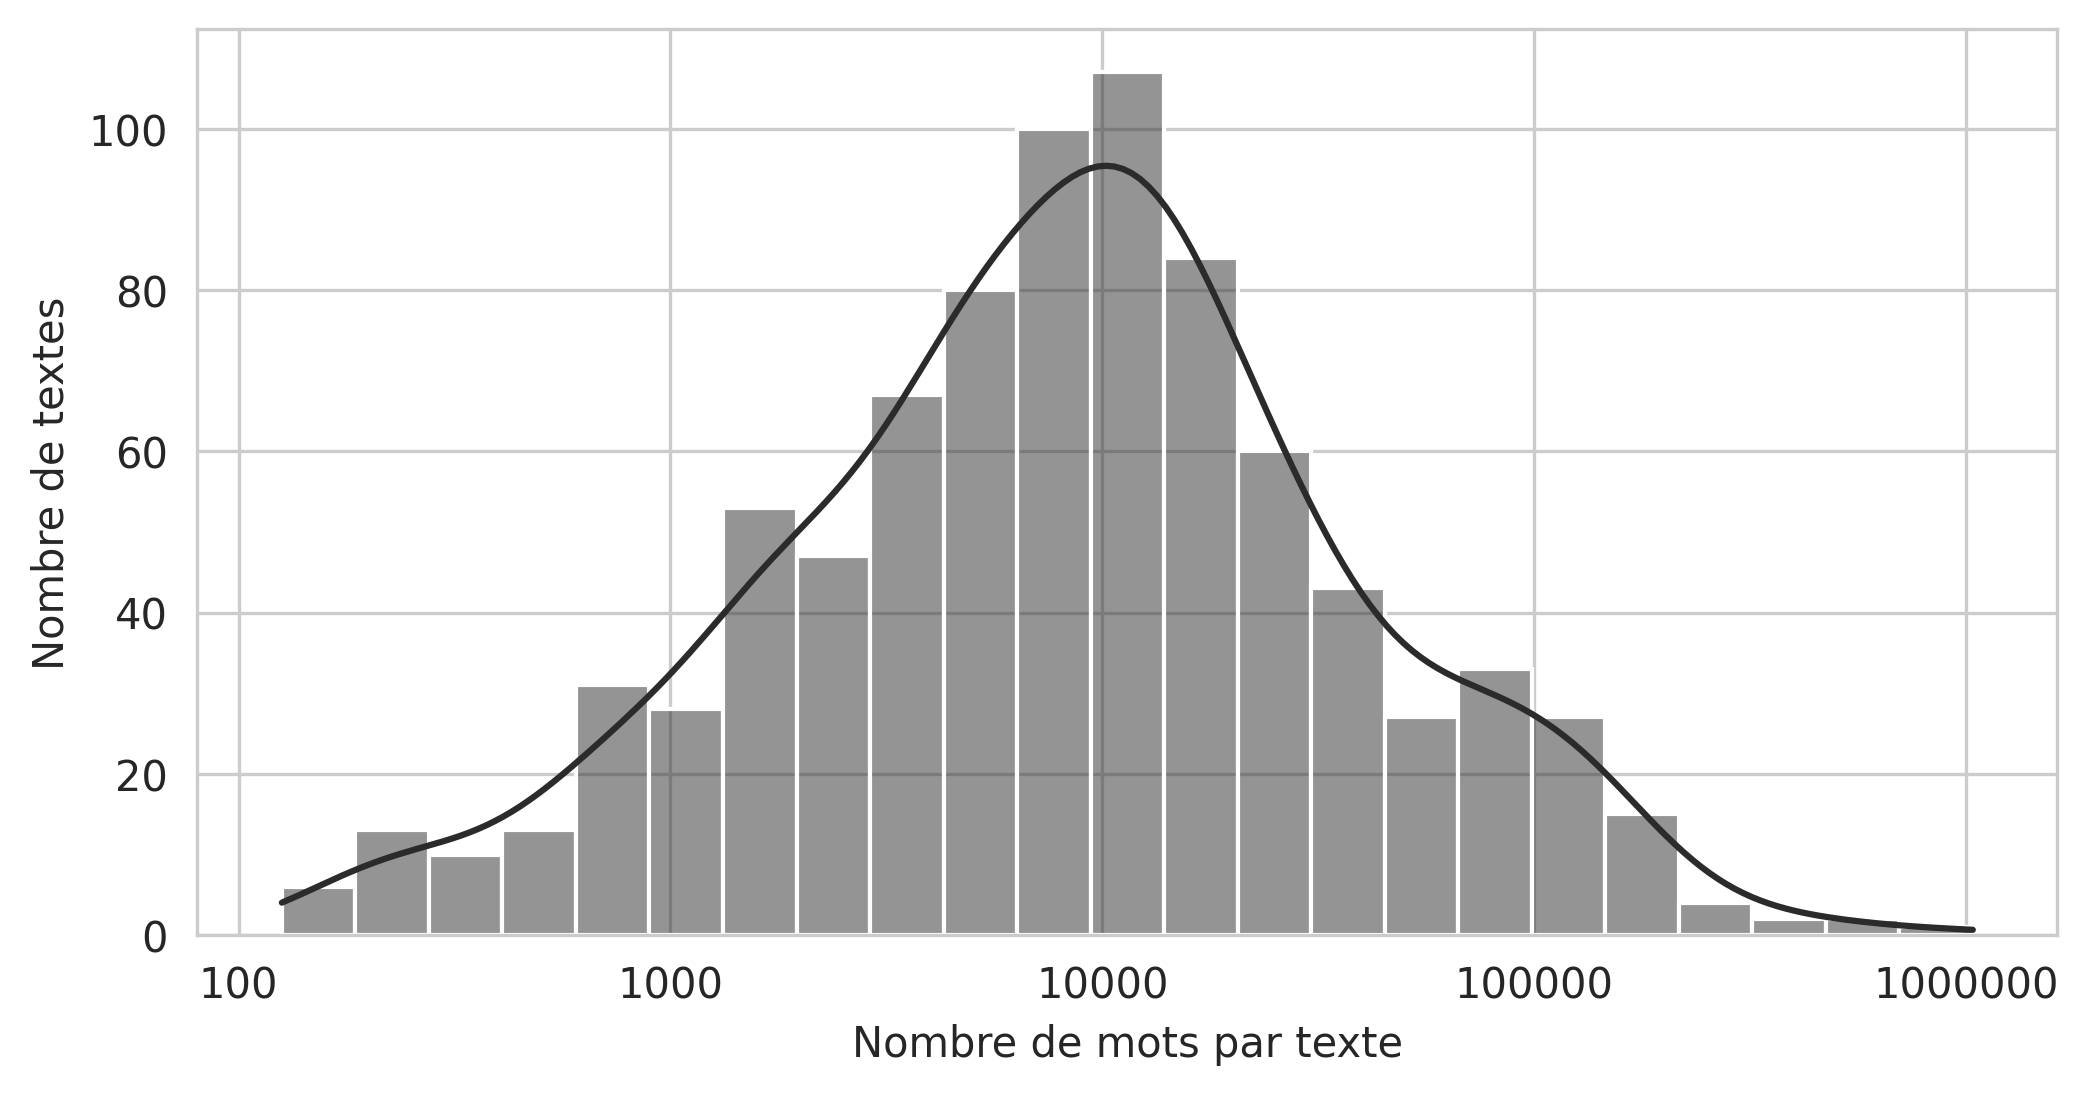
\includegraphics[width=.8\linewidth]{figures/chap1/part2/motsParTexte.png}
    \caption{Distribution des tailles de textes (en nombre de mots).}
    \label{fig:chap1:mots-par-texte}
\end{figure}
\begin{table}[]
    \centering
    \small
    \begin{tabular}{lrrrrrrrr}
    \toprule
    {} &  œuvres &          Moyenne &           std &    min &     25\% &     50\% &      75\% &        max \\
    \midrule
    Mots &  853 &  25003 &  59386 &  126 &  3~188 &  8~697 &  20~639 &  1~036~035 \\
    \bottomrule
    \end{tabular}
    \caption{Détails sur la répartition des tailles de textes}
    \label{tab:chap1:mots-par-textes}
\end{table}
\begin{figure}
    \centering
    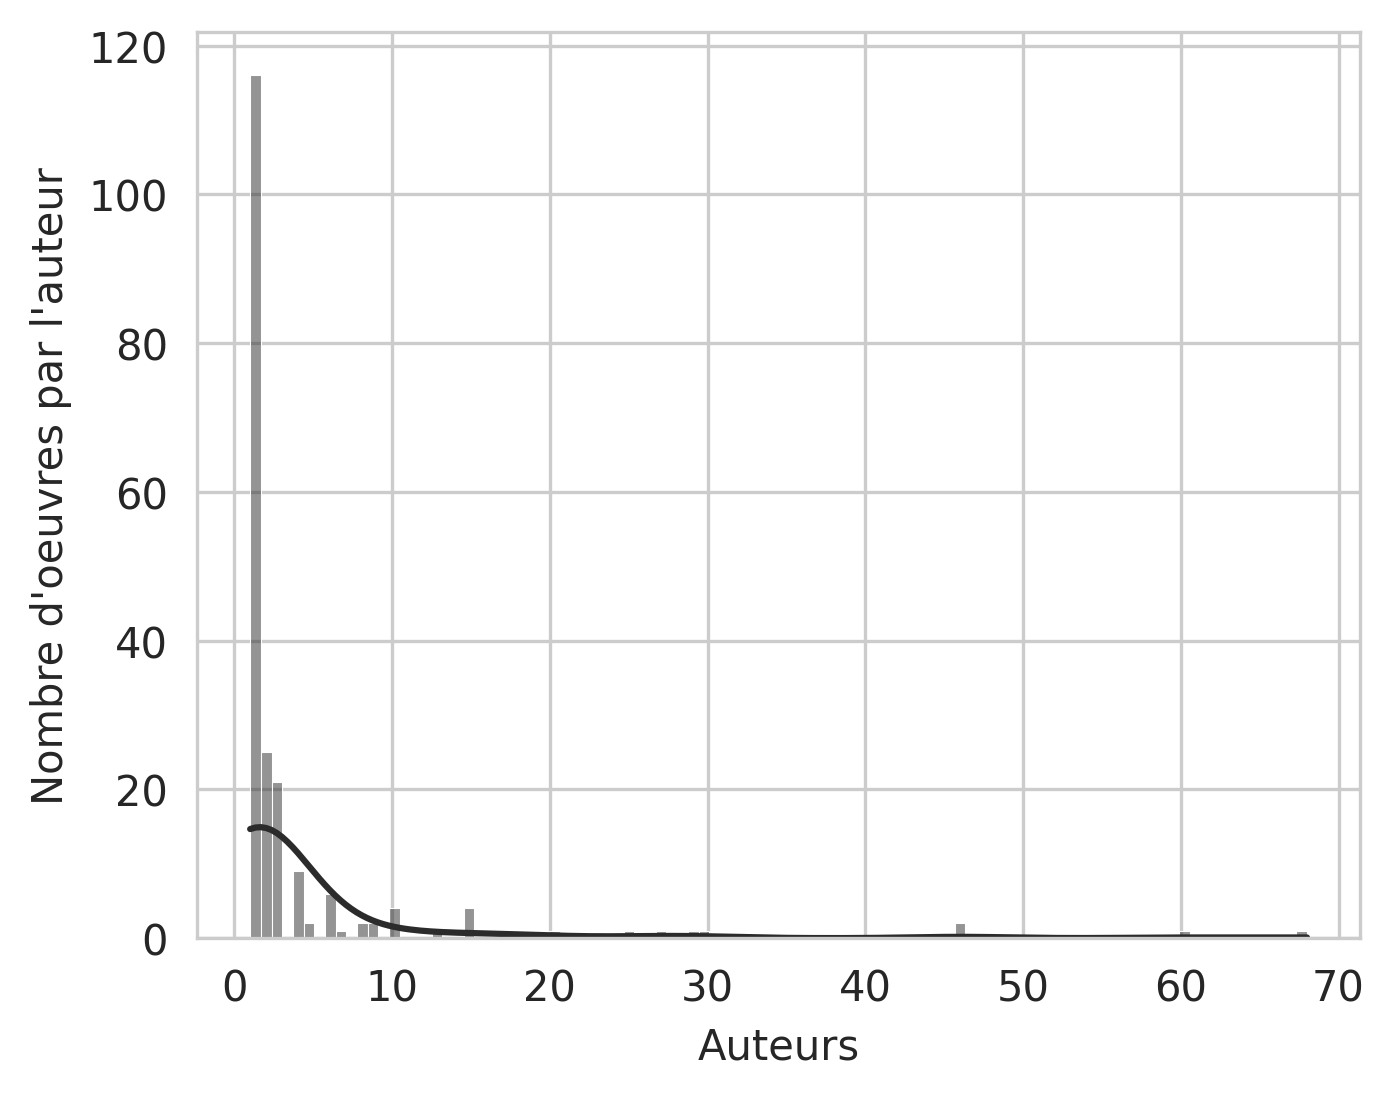
\includegraphics[height=8cm]{figures/chap1/part2/oeuvresParAuteur.png}
    \caption{Distribution du nombre d'œuvres par auteurs. Les chiffres sont partiellement faussés par la segmentation de la bible en livres, produisant une œuvre par livre.}
    \label{fig:chap1:œuvres-par-auteur}
\end{figure}
\clearpage
}

\afterpage{%
\begin{sidewaysfigure}%
%\begin{figure}
    \begin{subfigure}{0.45\hsize}
        \centering
        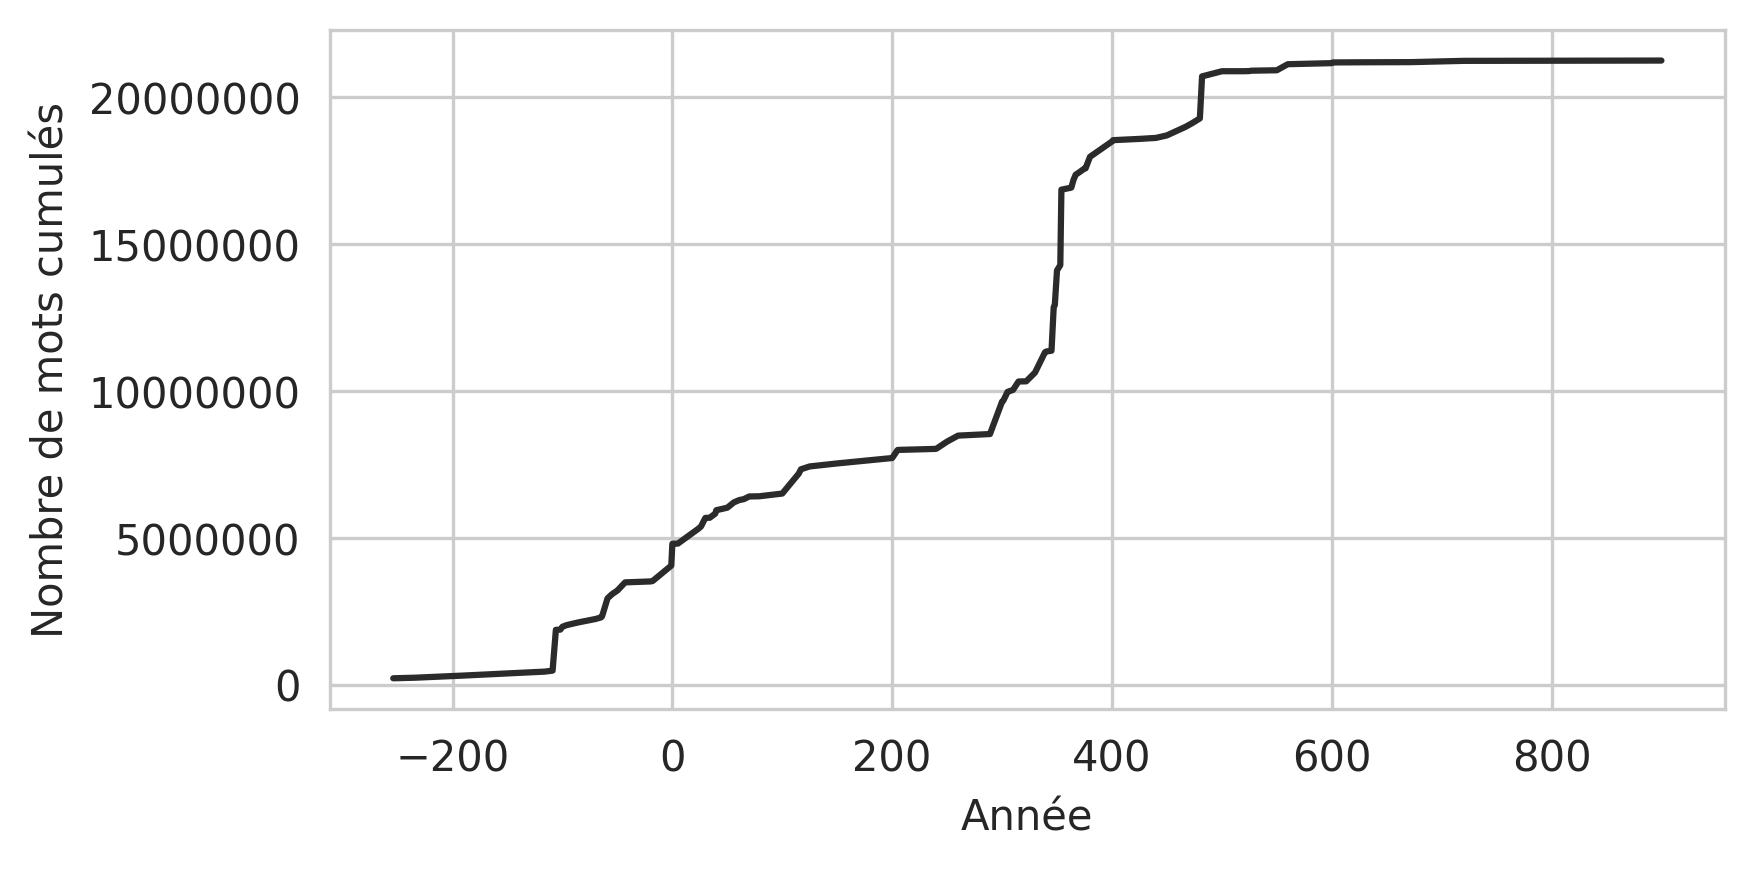
\includegraphics[width=\linewidth]{figures/chap1/part2/AccumulationMots.png}
        \caption{Accumulation générale du nombre de mots}
        \label{fig:chap1:accum-mot}
    \end{subfigure}%
    \hfill%
    \begin{subfigure}{0.45\hsize}
        \centering
        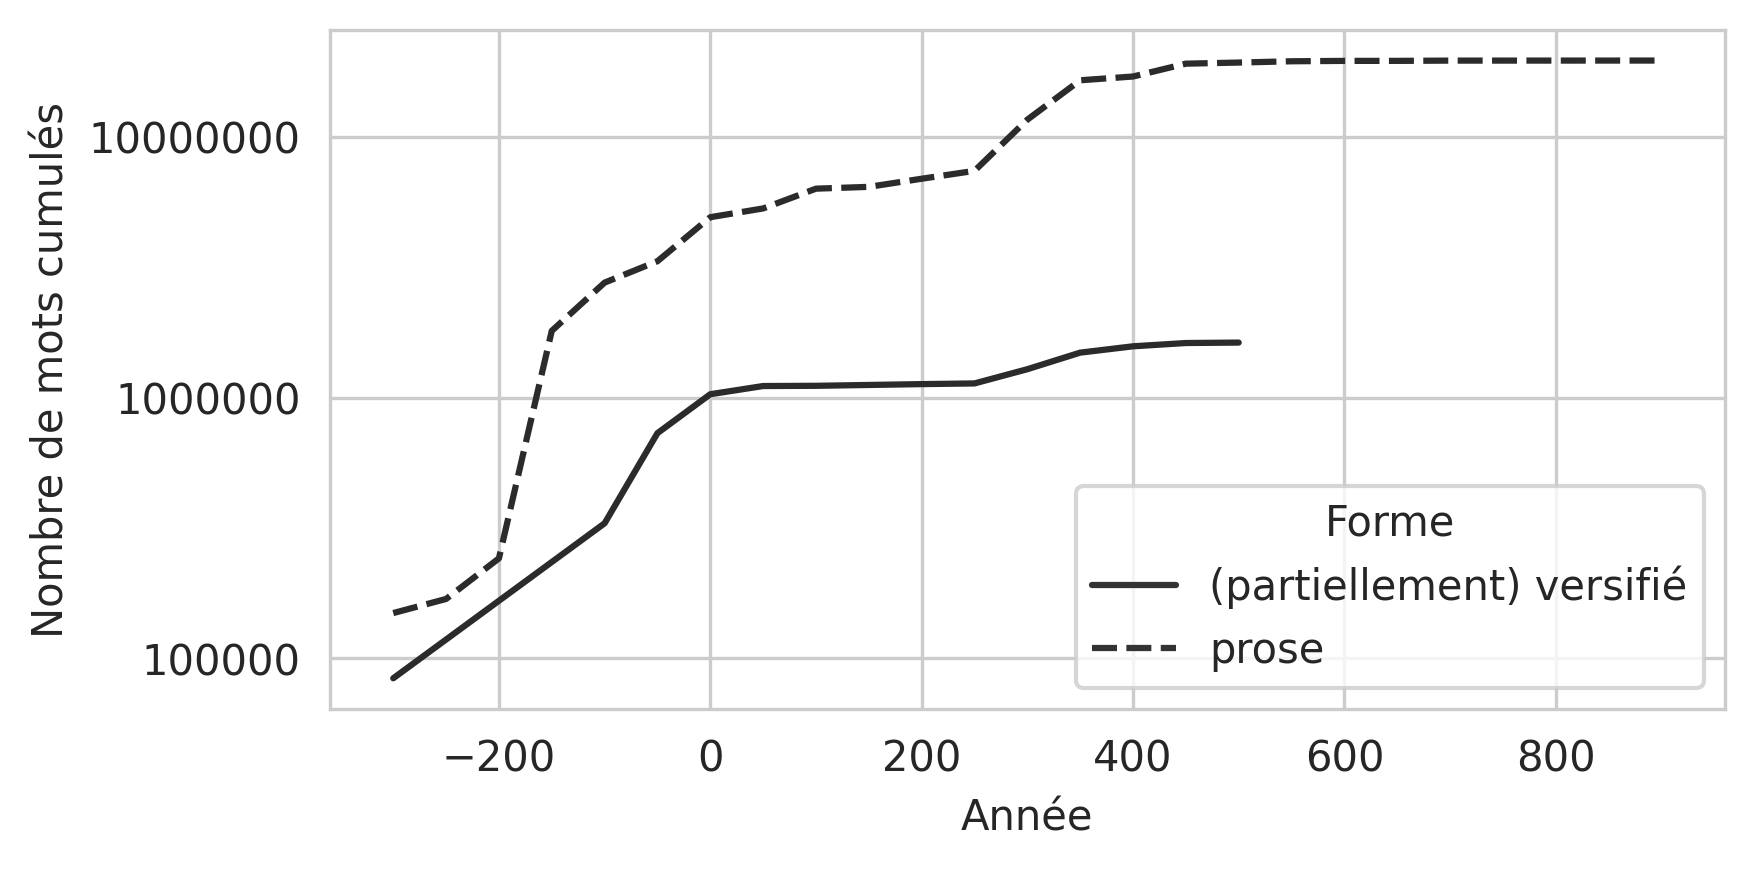
\includegraphics[width=\linewidth]{figures/chap1/part2/AccumulationMotsForme.png}
        \caption{Accumulation en fonction de la forme.}
        \label{fig:chap1:accum-mot-formes}
    \end{subfigure}%
    \vskip\baselineskip%
    \begin{subfigure}{0.45\hsize}
    \centering
    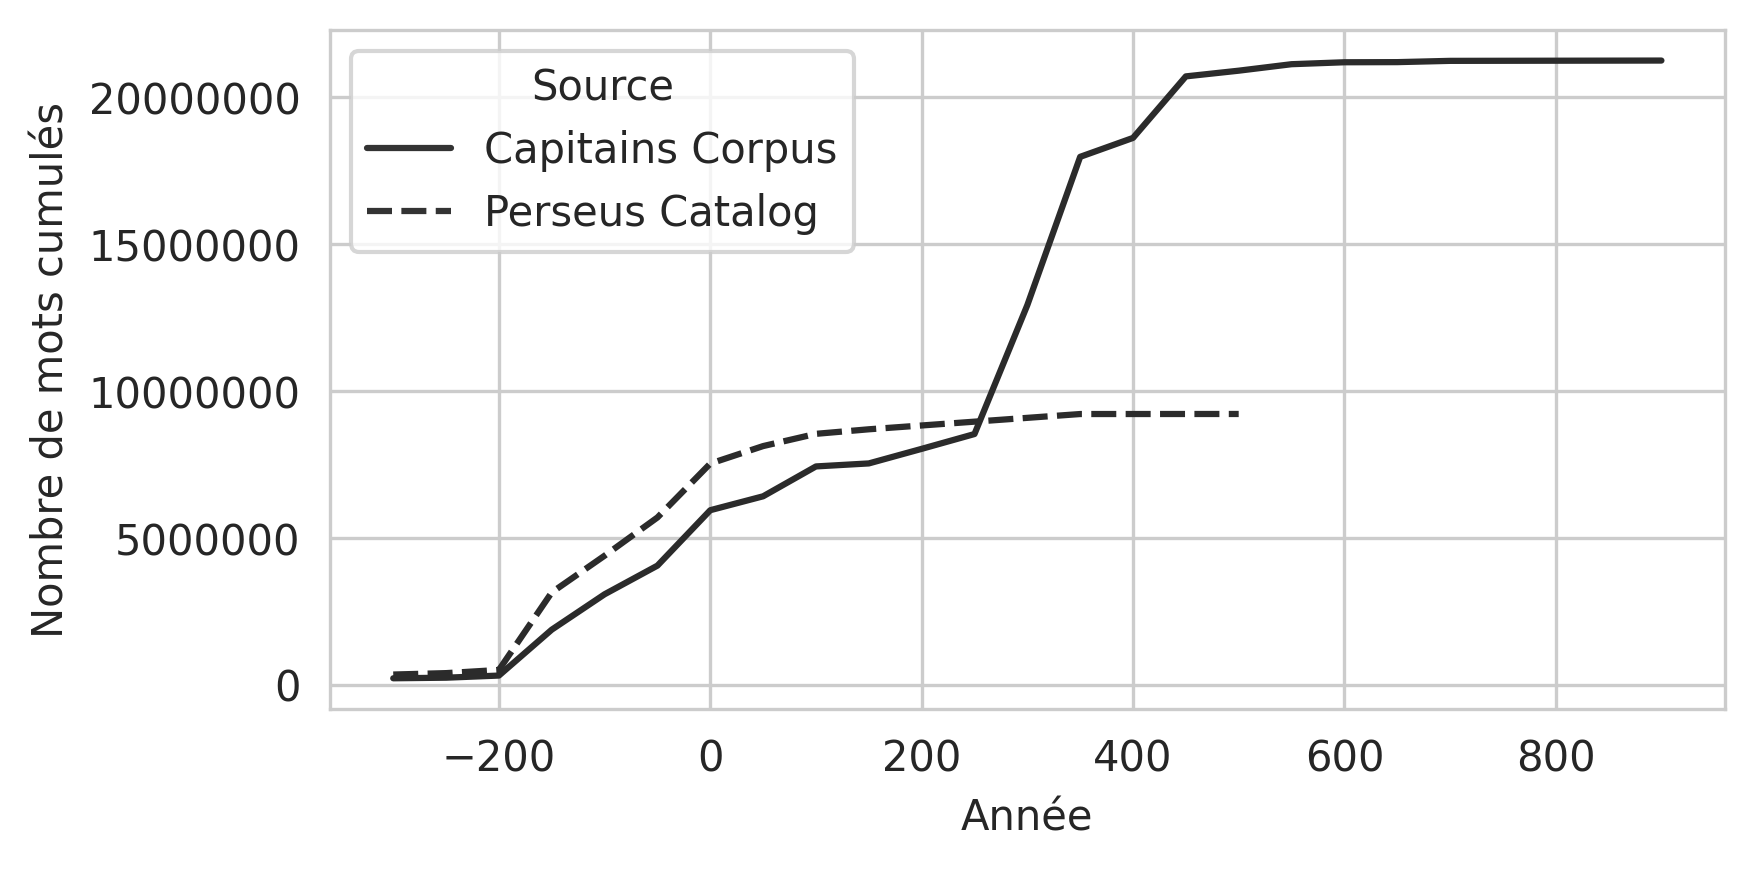
\includegraphics[width=\linewidth]{figures/chap1/part2/CatalogPerseusVSCapitains.png}
    \caption{Décompte de mots du \textit{Perseus Catalog} et de notre corpus.}
    \label{fig:chap1:accum-mot-diff-perseus-catalog}
    \end{subfigure}%
    \hfill%
    \begin{subfigure}{0.45\hsize}
        \centering
        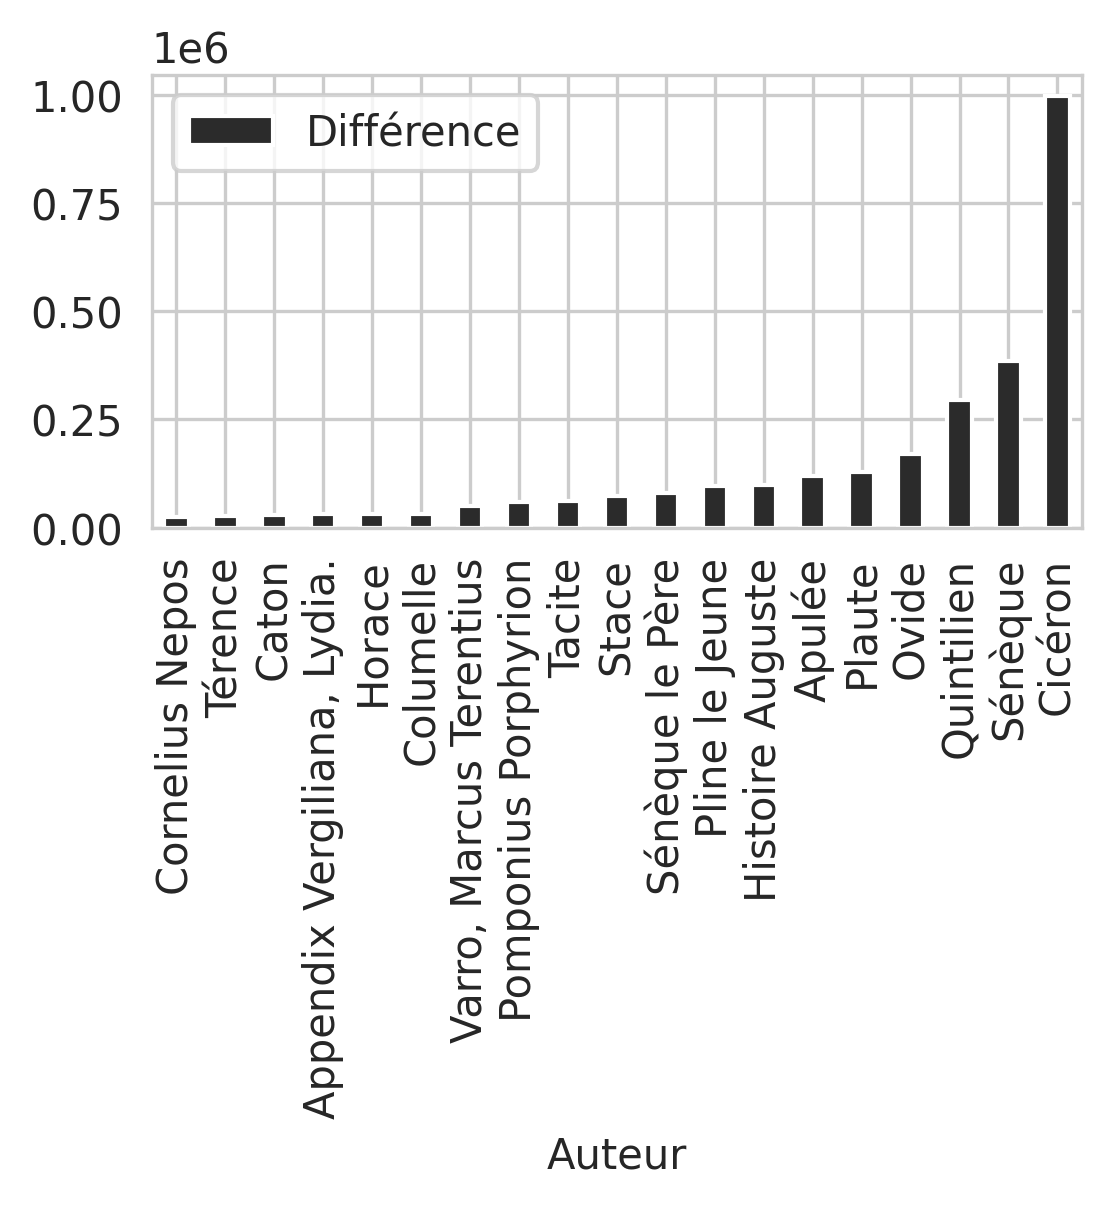
\includegraphics[width=.8\linewidth]{figures/chap1/part2/ecartsAuteurs.png}
        \caption{Écart supérieurs à 25~000 mots en défaveur de notre corpus en fonction du décompte de mots du catalogue de Perseus.}
        \label{fig:chap1:ecarts-auteurs}
    \end{subfigure}%
    \caption{Évolution de la masse du corpus. La date de composition utilisée est celle de la date de naissance présumée de l'auteur.}
\end{sidewaysfigure}%
\clearpage
}
% Le corpus final, une fois aggloméré
\clearpage

\subsection{Du corpus au document: qu’est-ce qu’un document pour l’ordinateur ?}

Nous avons vu que le corpus numérique latin, disponible dans des formats acceptables, dépasse de loin le méta-corpus accumulé ici, ne serait-ce qu'avec la \textit{Patrologia Latina} et \textit{DigilibLT}. Or, ces textes ont été laissés de côté au profit d'un corpus suivant intégralement les normes \textit{Capitains}, dont l'encodage est coûteux en temps. Nous proposons d'évaluer l'importance que peut avoir cette segmentation structurelle et son exploitabilité à travers une simple expérience: évaluer l'impact, dans une étude statistique des co-occurrents, de la prise en compte des segmentations structurelles \textit{machine actionable} de \textit{Capitains}. Dans un premier temps, nous définirons les catégories d'anlyses de cette expérience, à travers son héritage en linguistique de corpus, mais aussi à travers une définition de ce qu'est une rupture dans un \enquote{flux textuel}. Dans un second temps, nous définirons la méthode d'évaluation des corpus. Enfin, nous étudierons la différence entre les résultats des analyses effectuées\footnote{Ce texte a été réutilisé dans la publication en cours, \enquote{Thibault Clérice. \textit{"Don't worry, it's just noise": quantifying the impact of files treated as single textual units when they are really collections}}.}.

\subsubsection{Concepts}

\enquote{On reconnaît un mot à ceux qui l'accompagnent.\footnote{\enquote{\textit{You shall know a word by the company it keeps }}\textcite{firth_papers_1957}}.} Cette phrase de J. R. Forth, publiée en 1957, est devenue une citation classique pour définir la sémantique distributionnelle: pour trouver et comprendre le sens d'un ``mot'', on s'intéresse à ses co-occurrents.. Dans des phrases à trous telles que \enquote{Ce matin, j'ai bu un jus {[TROU]}}, il est facile de proposer des mots qui s'y retrouveraient logiquement, au premier titre desquels on aurait \enquote{d'orange}, car le contexte restreint drastiquement ce qui peut convenir après \enquote{jus}. Or, ce principe de sémantique distributionnelle est devenu si important qu'on le retrouve employé dans un très grand nombre d'outils, sans pour autant que la question de ce que forme une \enquote{compagnie} y soit remise en question\footnote{On trouve aussi le terme de \textit{voisinage} ou bien sûr de contexte en ce sens.}. Cette approche du lexique est très utilisée dans les domaines du latin et du grec ancien de la littérature classique\footcite{gillivray_greek}, tardo-antique\footcite{munson_biblical_2017}, médiévale\footcite{guerreau_pourquoi_1989,perreaux:eau} et \enquote{post-médiévale\footcite{bloem-etal-2020-distributional}} avec des corpus allant de quelques dizaines de milliers de mots à quelques millions. Mais bien souvent, les question du format des corpus et du traitement de ces format sont ignorées des descriptions des processus d'analyse, et ce qui constitue le contexte est défini majoritairement par une mesure: la fenêtre de capture de cette compagnie, c'est-à-dire le nombre de mots à gauche et à droite. 

Nous faisons l'hypothèse qu'ignorer les ruptures inhérentes aux œuvres numérisées peut porter préjudice à la sémantique distributionnelle, d'autant plus sur des petits corpus comme le nôtre (à peine vingt millions de mots), alors que d'autres comme celui tiré de \textit{Wikipedia France} ou OSCAR (plurilingue, cent cinquante-six langues représentées) atteignent respectivement un milliard et demi et huit cents milliards\footcite{noauthor_statistiques_nodate, ortizsuarez:hal02148693}. Parce que les œuvres numérisées sont bien souvent des calques de la transmission papier, elles tiennent parfois plus de la collection d'œuvres, comme les recueils d'épigrammes ou de poésie en général, que d'une œuvre \enquote{simple}. Dans le cadre d'un commentaire d'une épigramme de Martial, il ne viendrait pas à l'idée d'un latiniste de s'appuyer sur les premiers mots de l'épigramme suivante: bien qu'il arrive qu'une unité thématique joigne quelques poèmes chez Martial, ce sont des œuvres courtes et indépendantes les unes des autres. Or, si l'on traite un corpus de textes bruts ou de TEI sans faire attention au rôle des divisions structurelles, c'est exactement ce que la machine fait.

Nous avons vu précédemment que les œuvres présentaient une grande variation de contenus, du discours juridique à la collection de recettes chez Apicius. Ces textes sont formés par différents niveaux de segmentation structurelle, du chapitre pour les ouvrages d'histoire par exemple aux sections pour les grands discours, en passant bien sûr par les poèmes, les livres, les recettes, etc. Ces types de contenus sont parfois introduits par la transmission des textes, parfois d'origine, mais tous décrivent -- au moins partiellement -- la relation qui lie chacune de ces unités. Il est attendu qu'une recette et une autre recette ne se retrouvent voisines que \enquote{par hasard}, ou parce qu'elles sont toutes deux des recettes de viande, tandis que deux chapitres d'un ouvrage d'histoire formeront une probable continuité narrative.

Nous souhaitons alors qualifier ces unités dans deux grandes catégories. Il y a d'une part les \enquote{unités textuelles autonomes}~(\textit{Autonomous Textual Units}, ATU): ces unités marquent une rupture avec leurs voisines. Leur contenu ne pourrait être considéré comme co-occurrents d'un point de vue lexical et sémantique: le dernier mot d'une ATU ne peut être considéré comme suivi par le premier mot de l'ATU suivante. C'est le cas d'une très grande majorité de poèmes, des définitions des \textit{Étymologies} d'Isidore de Séville, des recettes d'Apicius, des commentaires ligne à ligne de Porphyrion. D'autre part, les autres unités peuvente être qualifiées d'\enquote{unités textuelles semi-autonomes}~(\textit{Semi-autonomous textual units}, SATU): ces unités présentent des continuités narratives, thématiques ou sémantiques entre elles. C'est le cas des vers, des sections, des chapitres, etc. Par exemple, cette semi-autonomie se manifeste par la difficile lecture d'une unité sans avoir pris en compte les précédentes, ou la présence d'ellipses narratives volontaires. Continuité et ruptures sont avant tout affaire de style avant d'être des traits caractérisants des (S)ATU.

Si l'on utilise des textes sans prendre en compte leurs structures, il est probable que des unités autonomes aient leur texte compté comme co-occurrent des unités voisines. Pour évaluer ce risque, on propose de mesurer un \enquote{taux théorique de contamination des fenêtres}. Pour un texte $t$, ce taux peut être calculé en fonction du nombre de (S)ATU du texte $\left | U_{t} \right |$, de la taille de la fenêtre utilisée $W$ et enfin du nombre de mots dans le texte $\left | t \right |$ tel que

\begin{equation*}
    Taux(t) = \left \{ %
    \begin{array}{ll}
         \frac{2W(\left|U_{t}\right| - 1)}{\left|t\right|} & \quad \text{si $\left|t\right| > 2W$} \\\\
         0 & \quad \text{sinon}
    \end{array} %
    \right .
\label{equation:twcr}
\end{equation*}

\noindent où chaque mot dans une (S)ATU est contaminé par un maximum de $2W$ mots co-occurrents tirés des (S)ATU voisines, à l'exception des toutes premières et dernières (S)ATU de l'œuvre ($\left|U\right| - 2 \times \frac{1}{2}$), qui n'ont qu'une unité voisine (d'où $\frac{1}{2}$). Ce taux représente la quantité relative de mots dont la fenêtre comporte au moins un voisin qui n'est pas censé être compté comme co-occurrent. Dans ce contexte, si l'on utilise les valeurs par défauts d'outils comme Gensim\footcite{vrehuuvrek2011gensim}, où la fenêtre est fixée à cinq ($W=5$), pour produire des analyses distributionnelles, et que l'on applique cette analyse à des œuvres comme celle de Martial, constituée de 1527 épigrammes pour 71~911 mots, ce taux théorique est de 21,22\%. La contamination pourrait donc s'étendre jusqu'à plus d'un mot sur cinq. Au contraire, sur des textes comme le \textit{Contre Pison} de Cicéron, constitué de sections qui ne forment pas de rupture et donc dont le texte est continu, le taux de contamination sera nul.

Si le taux de contamination théorique de la fenêtre constitue un outil efficace pour considérer la question, il considère que toute (S)ATU est de longueur égale, ce qui n'est bien évidemment jamais le cas. Le taux de contamination réel dépend à la fois de la taille des trois (S)ATU à considérer: la précédente, l'actuelle et la suivante. Dans le cas de très petits poèmes comme l'\textit{Épigramme} 3.40 de Martial (10 mots), pas une seule fenêtre n’est indemne de contamination si $W=5$. Pire encore, si la fenêtre adoptée est de dix mots, soit une fenêtre tout à fait plausible, chaque mot tire des co-occurrents des deux unités voisines en même temps (\textit{cf.} Figure~\ref{exc:epigrams}).

\begin{figure}
\small
\begin{minipage}[t]{0.45\textwidth}
(Poème~39)\\*
Iliaco similem puerum, Faustine, ministro\\*
Lusca Lycoris amat. Quam bene lusca videt!\\
(Poème~40)\\*
\textit{Inserta phialae Mentoris manu} \textbf{ducta}\\*
\textit{Lacerta vivit et timetur argentum}.\\
(Poème~41)\\*
Mutua quod nobis ter quinquagena dedisti\\*
Ex opibus tantis, quas gravis arca premit,\\* {[...]}
\end{minipage} \hfill
\begin{minipage}[t]{0.45\textwidth}
(Poème~39)\\*
Iliaco similem puerum, Faustine, ministro\\*
Lusca \textit{Lycoris amat. Quam bene lusca videt}!\\
(Poème~40)\\*
\textit{Inserta phialae Mentoris manu} \textbf{ducta}\\*
\textit{Lacerta vivit et timetur argentum}.\\
(Poème~41)\\*
\textit{Mutua quod nobis ter quinquagena} dedisti\\*
Ex opibus tantis, quas gravis arca premit,\\*  {[...]}
\end{minipage}
\caption{Livre 3, poèmes 39 à 40 des \textit{Épigrammes} de Martial. Les mots considérés comme co-occurrents de \textit{ducta} pour une fenêtre de dix mots ($W=10$) sont en italique. À gauche, le résultat attendu pour un lecteur humain, prenant en compte l'absence de continuité entre les deux poèmes. À droite, la même approche, mais en prenant l'œuvre comme une seule unité à analyser.}
\label{exc:epigrams}
\end{figure}


\subsubsection{Méthode d'évaluation}

Pour quantifier l'impact de la segmentation ou son absence, nous mettons en place toute une chaîne d'analyse permettant d'être reproduite facilement et de mettre en avant ces différences de traitement. Étant donné la particularité de l'approche -- les résultats de ces analyses ne nous intéressent pas directement, ce sont leurs différences qui sont importantes --, nous effectuons ces comparaisons à différents niveaux de traitement avec une grande variété de paramètres, souhaitant ainsi capturer plusieurs approches des textes.


\begin{figure}
    \centering
    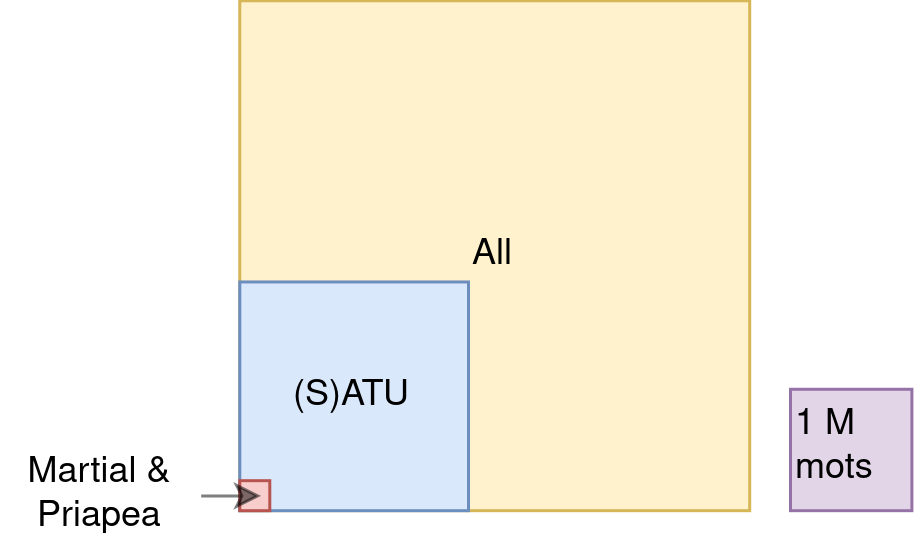
\includegraphics[width=0.6\linewidth]{figures/chap1/part2/VennCorpus.png}
    \caption{Représentation à l'échelle des trois sous-corpus et de leur relation les uns avec les autres : chaque corpus contient le ou les plus petits. }
    \label{fig:venn}
\end{figure}

Afin de quantifier l'effet de la segmentation ou de son absence, nous avons attribué à chaque texte un niveau auquel il doit être divisé, permettant ainsi de traiter les (S)ATU comme des unités non séquentielles. Pour les textes qui ne présentent pas de (S)ATU, par exemple un texte court formé de nombreux paragraphes, le texte complet a été conservé comme une seule unité. Nous produisons deux versions de chaque texte et donc de chaque corpus:
\begin{itemize}
    \item $S(T)$ (pour \textit{segment} de $T$, où $T$ est un corpus): les (S)ATU sont utilisées et les œuvres sont découpées en autant de textes indépendants. C'est le corpus segmenté.
    \item $U(T)$ (pour \textit{*unsegment} de $T$): les (S)ATU sont ignorées et toute œuvre présente en un seul fichier dans notre corpus est considérée comme une seule unité. C'est le corpus non segmenté.
\end{itemize}

Puis, nous divisons notre méta corpus en trois sous-corpus~(\textit{cf.} Figure~\ref{fig:venn}), représentant trois réalités différentes du point de vue des quantités, des thèmes ou encore des compositions des œuvres qui nous ont été transmises:
\begin{enumerate}
    \item Le premier corpus ne contient que les \textit{Épigrammes} de Martial et les \textit{Priapées} (\textit{Martial \& Priapea} ci-après). Ils forment un très petit corpus ($\left | t \right |=61~082$), avec des thèmes et des lexiques communs -- ils parlent tous deux de sexualité et de manière obscène la majeure partie du temps -- et sont des textes particulièrement composites. Le premier a une structure logique en trois niveaux (livre, poème, vers), le second en seulement deux niveaux (poème, vers). Ils sont composés de poèmes qui ne forment pas de séquences narratives et donc uniquement d'ATU.
    \item Le second, \textit{Corpus ATU} ci-après, est constitué de toutes les œuvres dans lesquelles il existe un niveau de la structure logique de citation qualifié de ``poème'', ``commentaire'' ou ``scholia'', ``lettre'', ``discours'' et ``entrée'' (on trouve ces dernières pour qualifier les recettes et les niveaux des \textit{Étymologies}): cela représente 125 œuvres et 3~549~249 mots. Ils ne forment pas d'unité thématique, mais sont tout de même majoritairement composés de poésie, y compris à travers les répétions dans les \textit{scholia}. Il comprend \textit{Martial \& Priapea}.
    \item Le dernier est le méta corpus complet avec ses 17~639~626 mots (\textit{All}) .
\end{enumerate}

Chaque corpus affiche une valeur différente de la propriété combinée ``Nombre d'(ATU)-Taille du corpus'' (\textit{cf.} table \ref{tab:chap1:noise:corpora_properties}). Le premier est un très petit corpus avec un nombre élevé d'unités textuelles autonomes. Le second a un nombre élevé d'ATU, mais atteint un plus grand nombre de mots. Le dernier est un mélange massivement construit de longs passages en petite quantité par œuvre, et seuls dix pour cent de ce corpus est riche en ATU.

\begin{table*}[ht!]
    \centering
    \resizebox{1\linewidth}{!}{%
    \begin{tabular}{l|rr|rr|rr|rrrrrrr}
    \toprule
    {} & \multicolumn{2}{l}{(S)ATU} & \multicolumn{2}{l}{Mots} & \multicolumn{2}{l}{œuvres} & \multicolumn{7}{l}{Distribution du ratio Mots / (S)ATU} \\
    {} &  Total &     \% &     Total &     \% & Total &     \% & Moy. &  Dév. & Min & 25\% & 50\% & 75\% &    Max \\
    \midrule
    \textit{Martial \& Priapea} &   1607 &   2,8 &     61~056 &   0m3 &     2 &   0m2  &  38 &   32 &   7 &  13 &  27 &  54 &    280 \\
    Corpus ATU        &  39~591 &  68,5 &   3~549~249 &  20,1 &   125 &  14,8 &  90 &  603 &   1 &   9 &  17 &  36 &  47~783 \\
    \textit{All}               &  57~761 & 100,0 &  17~639~626 & 100,0 &   845 & 100,0 & 305 & 2~159 &   1 &  11 &  24 &  77 & 248~564 \\
    \bottomrule
    \end{tabular}%
    }
    \caption{Propriétés des différents corpus. Les signes de ponctuation sont ignorés dans le décompte des mots.}
    \label{tab:chap1:noise:corpora_properties}
\end{table*}

% Reprendre ici
% \subsubsection{Analyse sémantique et dispositif expérimental}

Comme l'objectif principal est d'analyser l'impact de la segmentation du texte sur la sémantique distributionnelle, nous mettons en place l'expérience sur la base de quatre paramètres. Nous combinons ensuite ces paramètres pour produire des analyses en utilisant les deux versions de $T$ et comparer leurs résultats. Ces quatre paramètres représentent ensemble un assez grand nombre de variations permettant de contrôler les conditions dans lesquelles $Analyse(S(T)) \neq Analyse(U(T))$: il s'agit des groupes de mots étudiés, de la taille de la fenêtre de capture des co-occurrents, des fréquences minimales pour qu'un mot soit comptabilisé dans les analyses, et enfin du nombre de groupes que l'on veut produire par \textit{clusterisation}.

Pour les groupes de mots étudiés, on utilise des termes appartenant à des champs lexicaux identifiés (famille, poésie et écriture, sexualité) afin que leur séparation en sous-groupes soit nette quand nous les regroupons. Ces groupes de mots, que nous appelons pivots, présentent aussi des particularités en termes de fréquences -- ils apparaissent tous au moins dix fois -- et de spécificités génériques:

\begin{enumerate}
    \item Le premier, \textit{Puer et al.}, contient des mots liés au foyer romain et n'est spécifique à aucun des corpus. Il s'agit de \textit{dominus, mater, pater, puella, puer, uir, uxor}, qui sont présents entre 2~036 (\textit{puella}) à 48~519 fois (\textit{dominus}) dans \textit{All}.
    \item Le second, \textit{Carmen et al.}, pourrait être plus spécifique aux grammairiens et à la poésie, qui sont surreprésentés dans \textit{Corpus ATU}. Il contient \textit{scribo, poeta, libellus, lego2, carmen1, liber1} (\textit{cf. } Table \ref{tab:chap1:noise:freq_corpora})\footnote{Lorsque les lemmes se terminent par des chiffres comme \textit{lego2}, cela représente un indice de désambiguïsation : en latin, la première personne de l'indicatif présent est souvent utilisée pour représenter le lemme, mais deux verbes partagent la forme \textit{lego} : l'un est conjugué \textit{legis} à la deuxième personne (signifiant : lire, \textit{lego2}) tandis que l'autre devient \textit{legas} (signifiant : nommer, \textit{lego1})}. 
    \item Le troisième, \textit{Puer, Carmen et al.}, est une combinaison des deux premiers et offre en tant que telle deux sous-groupes sémantiques clairement distincts qui devraient être faciles à retrouver par lexicométrie.
    \item Le dernier, \textit{Futuo, Carmen, Puer et al.}, est une combinaison des deux premiers ainsi que des mots obscènes ou du moins liés à l'expression de la sexualité : pour certains, ils sont fortement spécifiques à \textit{Martial et Priapea}, ont une fréquence très faible par rapport au premier groupe, mais sont aussi quelque peu spécifiques à \textit{Corpus ATU}. Il s'agit de \textit{cunnus, fello, futuo, irrumo, lasciuus, mentula, paedico2} (\textit{cf.} table \ref{tab:chap1:noise:freq_corpora} pour chaque fréquence de mots selon le corpus).
    \item Afin d'évaluer le bruit avant l'analyse, nous considérons également un cinquième ensemble de mots composé des 1000 mots les plus fréquents du jeu de données \textit{All}. Seuls les adverbes, adjectifs, pronoms, noms ou verbes sont pris en compte pour former ce \textit{Top 1000}.
\end{enumerate}


\begin{table}[p]
    \centering
    \begin{tabular}{l|rrr|rrrr}
    \toprule
    {} &  \makecell{Martial \\ \& Priapea} &  ATU &       All &  \makecell{Puer \\ et al.} &  \makecell{Carmen \\ et al.} &  \makecell{Puer et Carmen \\ et al.} &  \makecell{Futuo \\ et al.} \\
    \midrule
cunnus   &                  33 &              42 &        43 &         &           &                   &                        $\checkmark$ \\
fello    &                  11 &              14 &        28 &         &           &                   &                        $\checkmark$ \\
futuo    &                  46 &              52 &        52 &         &           &                   &                        $\checkmark$ \\
irrumo   &                  10 &              16 &        16 &         &           &                   &                        $\checkmark$ \\
lasciuus &                  35 &             155 &       300 &         &           &                   &                        $\checkmark$ \\
mentula  &                  68 &              75 &        75 &         &           &                   &                        $\checkmark$ \\
paedico2 &                  17 &              20 &        22 &         &           &                   &                        $\checkmark$ \\
carmen1  &                  90 &            1~753 &      3~101 &         &           $\checkmark$ &                   $\checkmark$ &                        $\checkmark$ \\
lego2    &                  95 &            3~030 &     10~252 &         &           $\checkmark$ &                   $\checkmark$ &                        $\checkmark$ \\
libellus &                 119 &             546 &      1~190 &         &           $\checkmark$ &                   $\checkmark$ &                        $\checkmark$ \\
liber1   &                  36 &            1~773 &     21~015 &         &           $\checkmark$ &                   $\checkmark$ &                        $\checkmark$ \\
poeta    &                  53 &            1~366 &      2~944 &         &           $\checkmark$ &                   $\checkmark$ &                        $\checkmark$ \\
scribo   &                  71 &            6~282 &     20~501 &         &           $\checkmark$ &                   $\checkmark$ &                        $\checkmark$ \\
dominus  &                 112 &            \textbf{7~420} &     \textbf{48~519} &         $\checkmark$ &           &                   $\checkmark$ &                        $\checkmark$ \\
mater    &                  43 &            2~132 &      9~271 &         $\checkmark$ &           &                   $\checkmark$ &                        $\checkmark$ \\
pater    &                  73 &            5~154 &     29~927 &         $\checkmark$ &           &                   $\checkmark$ &                        $\checkmark$ \\
puella   &                 120 &             989 &      2~036 &         $\checkmark$ &           &                   $\checkmark$ &                        $\checkmark$ \\
puer     &                 \textbf{159} &            1~812 &      5~824 &         $\checkmark$ &           &                   $\checkmark$ &                        $\checkmark$ \\
uir      &                  94 &            3~908 &     20~062 &         $\checkmark$ &           &                   $\checkmark$ &                        $\checkmark$ \\
uxor     &                  63 &            1~306 &      7~832 &         $\checkmark$ &           &                   $\checkmark$ &                        $\checkmark$ \\
    \bottomrule
    \end{tabular}

    \caption{Distribution des fréquences des lemmes sur les trois sous-corpus. En gras les plus hautes valeurs}
    \label{tab:chap1:noise:freq_corpora}
\end{table}


Nos deuxièmes et troisièmes paramètres sont la taille de la fenêtre, $W$, et notre seuil plancher de fréquence, $F$. $W$ varie parmi quatre valeurs ($\left [ 5, 10, 15, 20 \right ]$), capturant ainsi différentes formes de contexte: des mots immédiatement à côté de notre terme étudié à ceux dans les phrases ou ensembles syntaxiques autour de ce dernier. Pour $F$, on filtre le bruit en ne considérant que les mots qui ne sont présents qu'au moins $F$ fois dans les contextes récupérés: si \texttt{lemma1} apparaît $2$ fois avec \texttt{pivot1} et $5$ fois avec \texttt{pivot2}, il est conservé comme caractéristique si $F\geq5$. $F$ est sélectionné parmi $\left [ 1, 5, 10, 20 \right ]$: plus le nombre est haut, moins le bruit statistique sera important, les co-occurrences uniques seront ignorées lorsque $F > 1$ par exemple.


En utilisant toutes les combinaisons de $W$ et $F$ (16 combinaisons possibles par sous-corpus, soit 48 expériences), on passe les quatre premiers ensembles de mots à travers un même ensemble de traitements\footnote{\textit{Top1000} n'est pas utilisé dans toute l'expérience, voir ci-dessous.}:
\begin{enumerate}
    \item Nous récupérons la fréquence des co-occurrences dans une matrice où elles constituent des caractéristiques et où les pivots forment des classes. Cette matrice nous permet d'opérer à une première comparaison entre des décomptes bruts des $U(T)$ et $S(T)$.
    \item Suivant le travail de S. Evert\footcite{evert2005statistics}, A.~Guerreau chez J.~Morsel\footcite{morsel:guerreau} et N.~Perreaux\footcite{perreaux:cbma}, nous appliquons un algorithme de normalisation appelé coefficient de \textit{Dice}. L'usage de ce coefficient permet de faire ressortir les caractéristiques les plus importantes de chaque classe.
    \item Pour chaque pivot, nous gardons leurs 5 caractéristiques les plus corrélées. Si plusieurs termes se retrouvent en cinquième place, ils sont tous considérés. Ces caractéristiques forment un deuxième ensemble de mots que nous appelons \textit{co-occurrences majeures} ($M$).
    \item Nous récupérons et augmentons la matrice originale à l'étape 1 avec la même stratégie de récupération et de stockage pour chaque mot de $M$. Les classes sont désormais formées des \textit{pivots} et de $M$.
    \item Nous normalisons à nouveau la sortie avec le coefficient de \textit{Dice}.
\end{enumerate}

C'est à ce moment de la chaîne qu'intervient notre quatrième paramètre, le nombre de groupes. La matrice normalisée finale peut être utilisée afin de produire une \textit{clusterisation}, c'est-à-dire un regroupement de classes. Nous avons utilisé un très classique \textit{clustering} agglomératif de Ward\footcite{ward1963hierarchical} à base de distances euclidiennes. Afin de pouvoir comparer les résultats du clustering sur $U(T)$ et $S(T)$, nous harmonisons les co-occurrences majeures en supprimant celles qui ne sont pas partagées entre les analyses effectuées avec les mêmes paramètres sur les deux versions de $T$. Cela produit un ensemble de classes communes $C$ qui peuvent finalement être regroupées selon un quatrième paramètre $k$, où $k$ est le nombre de \textit{clusters} que nous voulons obtenir. Nous faisons varier $k$ de sorte que $\frac{\left | C \right |}{k} < 2$ et $5 \geq k < 15$. L'étude de la variation étant l'objectif de cet article, le nombre de \textit{clusters} n'a pas besoin d'être affiné, puisque nous nous intéressons uniquement à l'égalité ou l'inégalité entre l'analyse de $U(T)$ et $S(T)$.


\subsubsection{Évaluation de l'impact}

Une fois que toutes les combinaisons et chaînes de traitement ont été exécutées, nous voulons évaluer trois différents types de différences potentielles entre les résultats de $U(T)$ et $S(T)$: un premier effet brut sur les éléments trouvés dans les contextes des groupes de mots qui forment les caractéristiques de chaque pivot, un deuxième effet sur la sélection des classes secondaires (co-occurrences majeures), impliquant donc un traitement de normalisation, et enfin l'effet sur une analyse plus avancée, le \textit{clustering}.

\paragraph{Sur la matrice de co-occurrence}
\label{chap1:noise:par:manhattan}

Pour quantifier l'impact de l'absence de segmentations structurelles sur la récupération de contexte, nous opérons d'abord à une analyse des différences assez brutes. Nous utilisons pour cela une simple distance de Manhattan entre les vecteurs de chaque pivot dans les versions segmentées et non segmentées du corpus. Ce calcul de distance est effectué pour chaque combinaison $W$ et $F$. Comme certaines caractéristiques pourraient être absentes de l'une ou l'autre des matrices, leur fréquence avec le pivot concerné est estimée à 0.

\begin{figure}[ht]
    \centering
    \begin{minipage}{.49\linewidth}%
        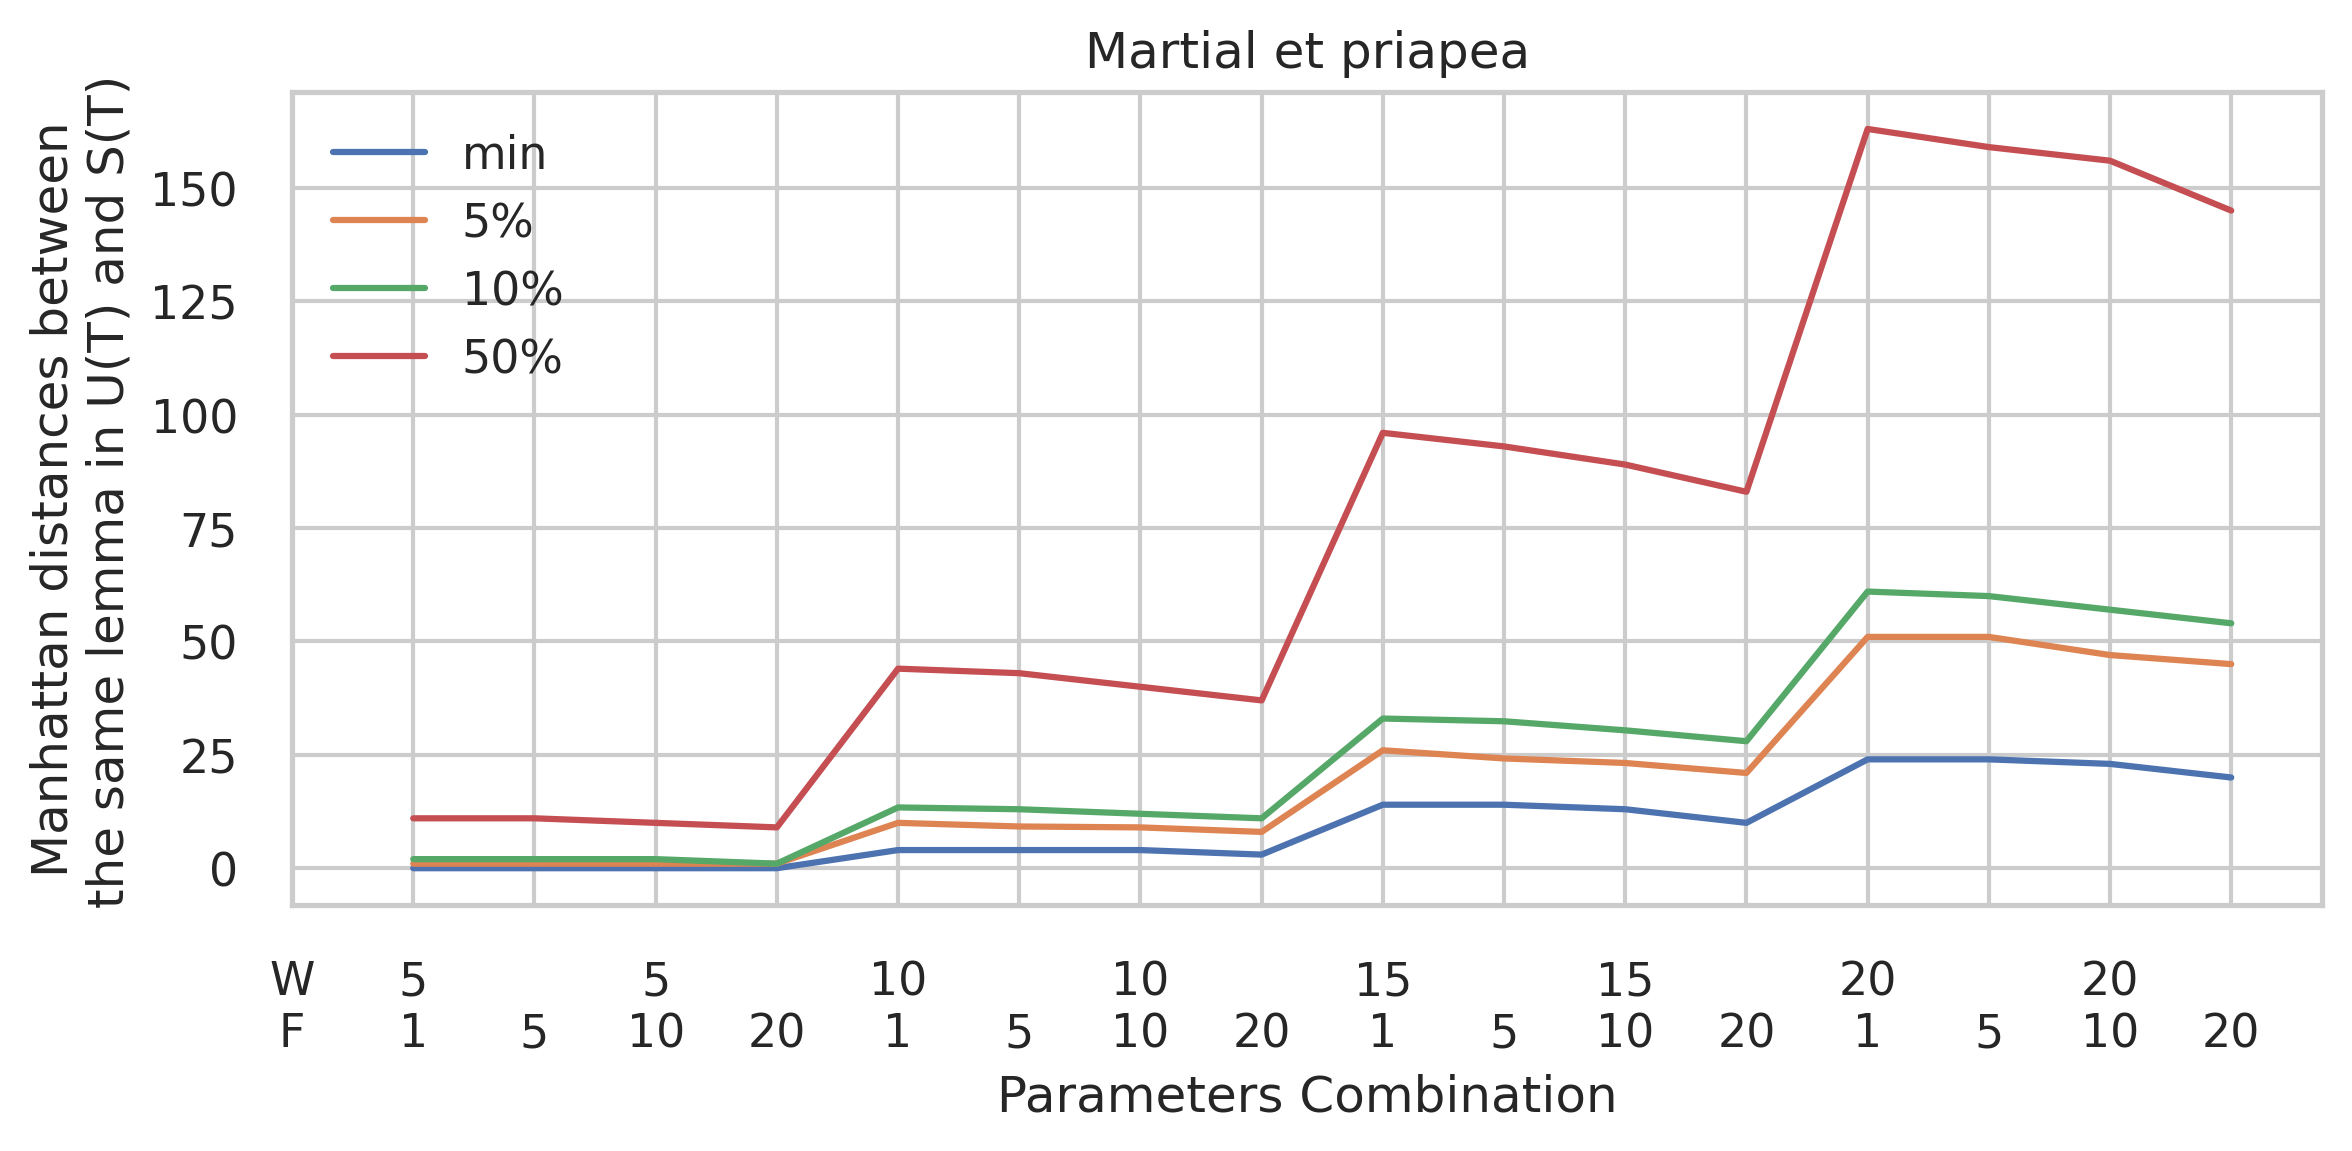
\includegraphics[width=1\linewidth]{figures/chap1/part2/manhattan_martial.png} 
    \end{minipage}%
    \hfill
    \begin{minipage}{.49\linewidth}
        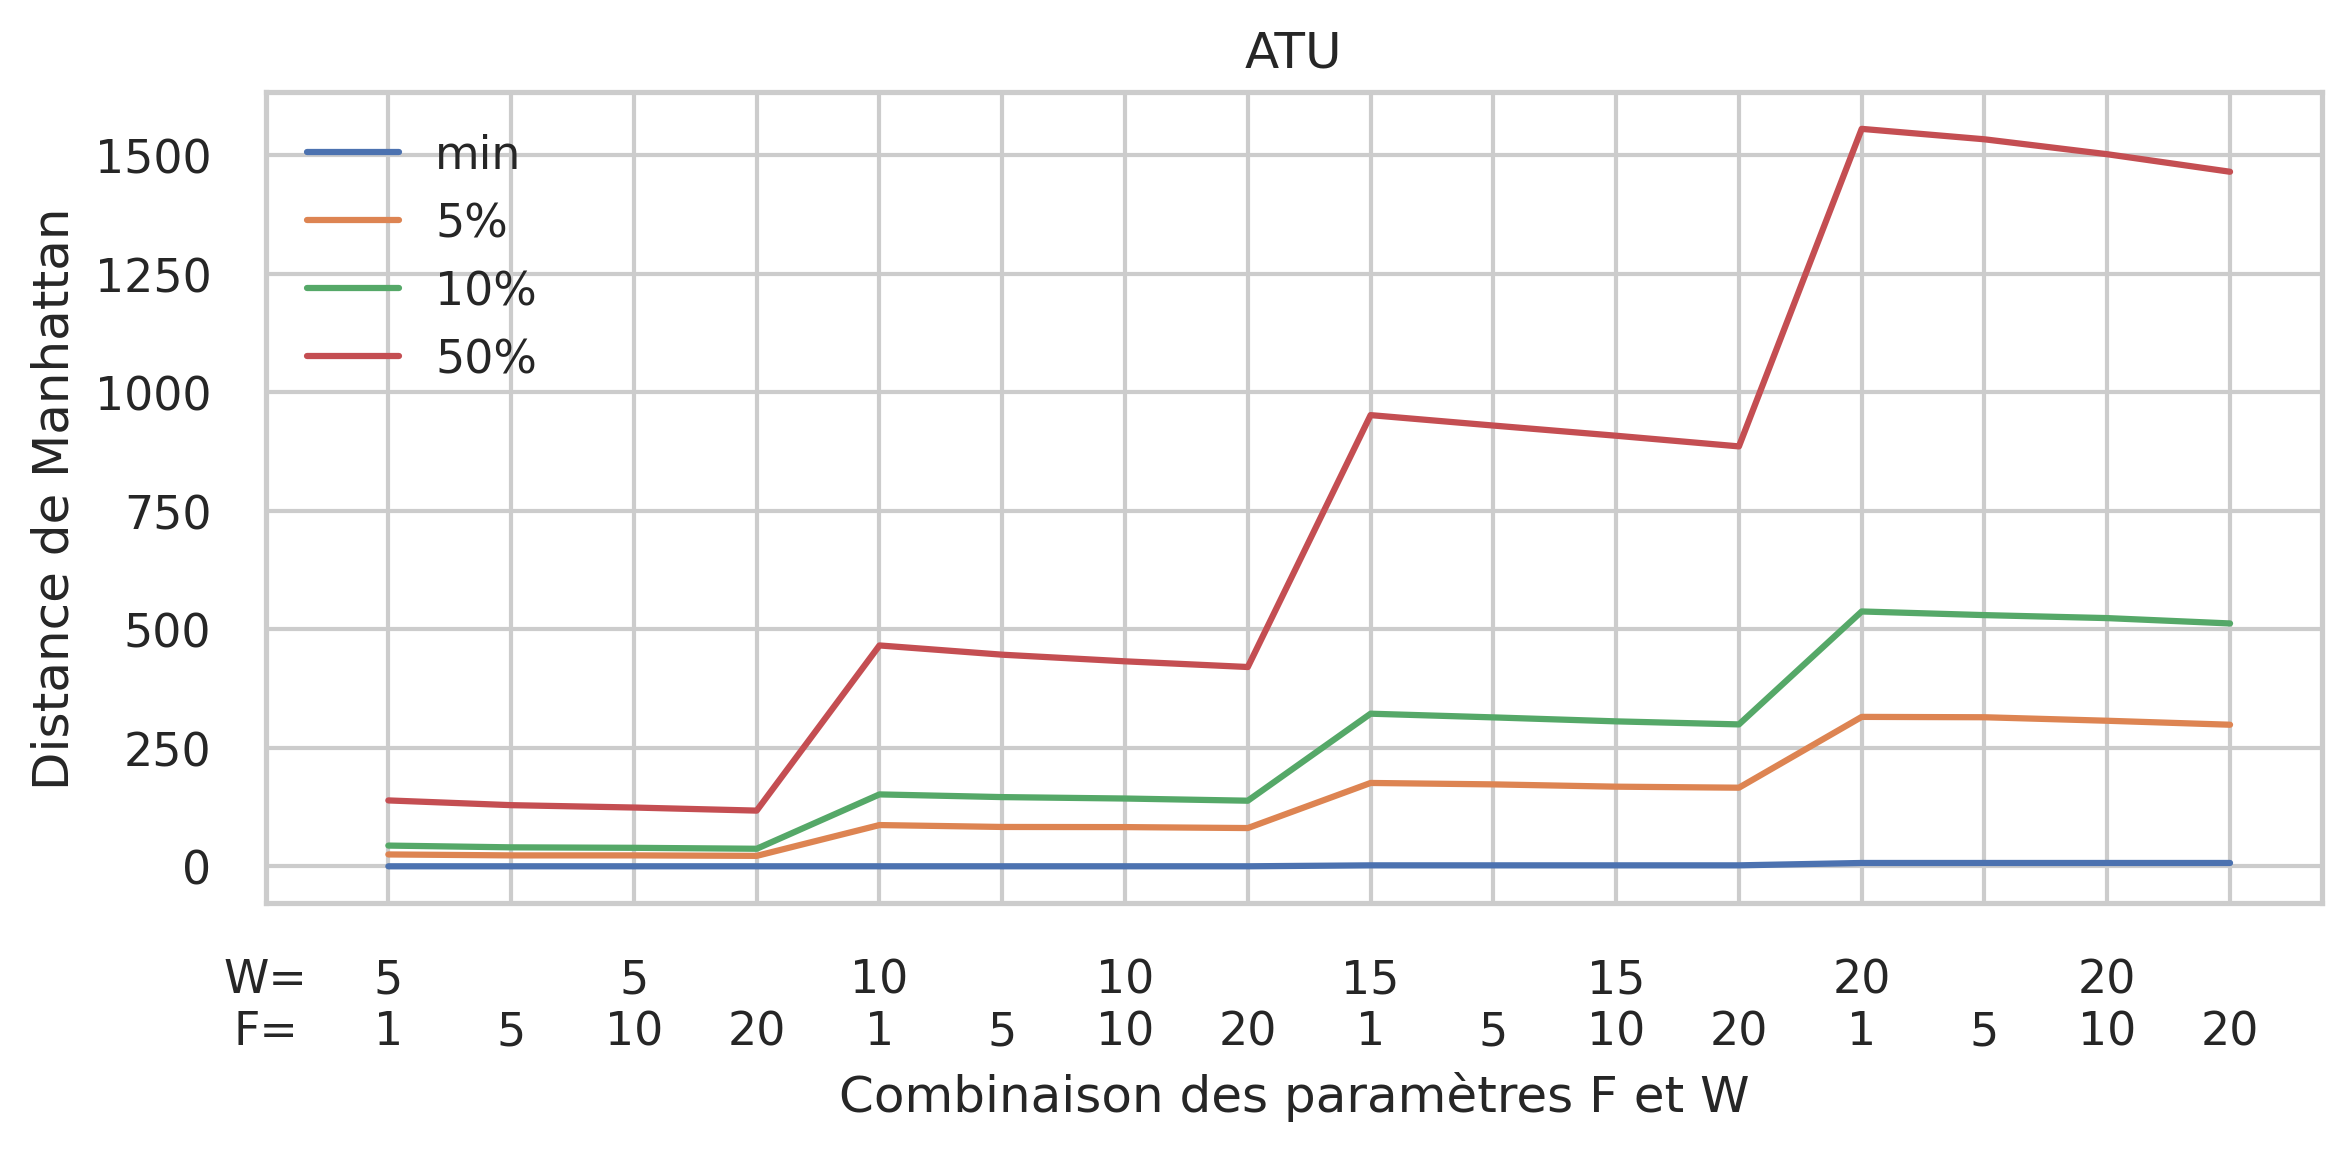
\includegraphics[width=1\linewidth]{figures/chap1/part2/manhattan_ATU.png}
    \end{minipage}
    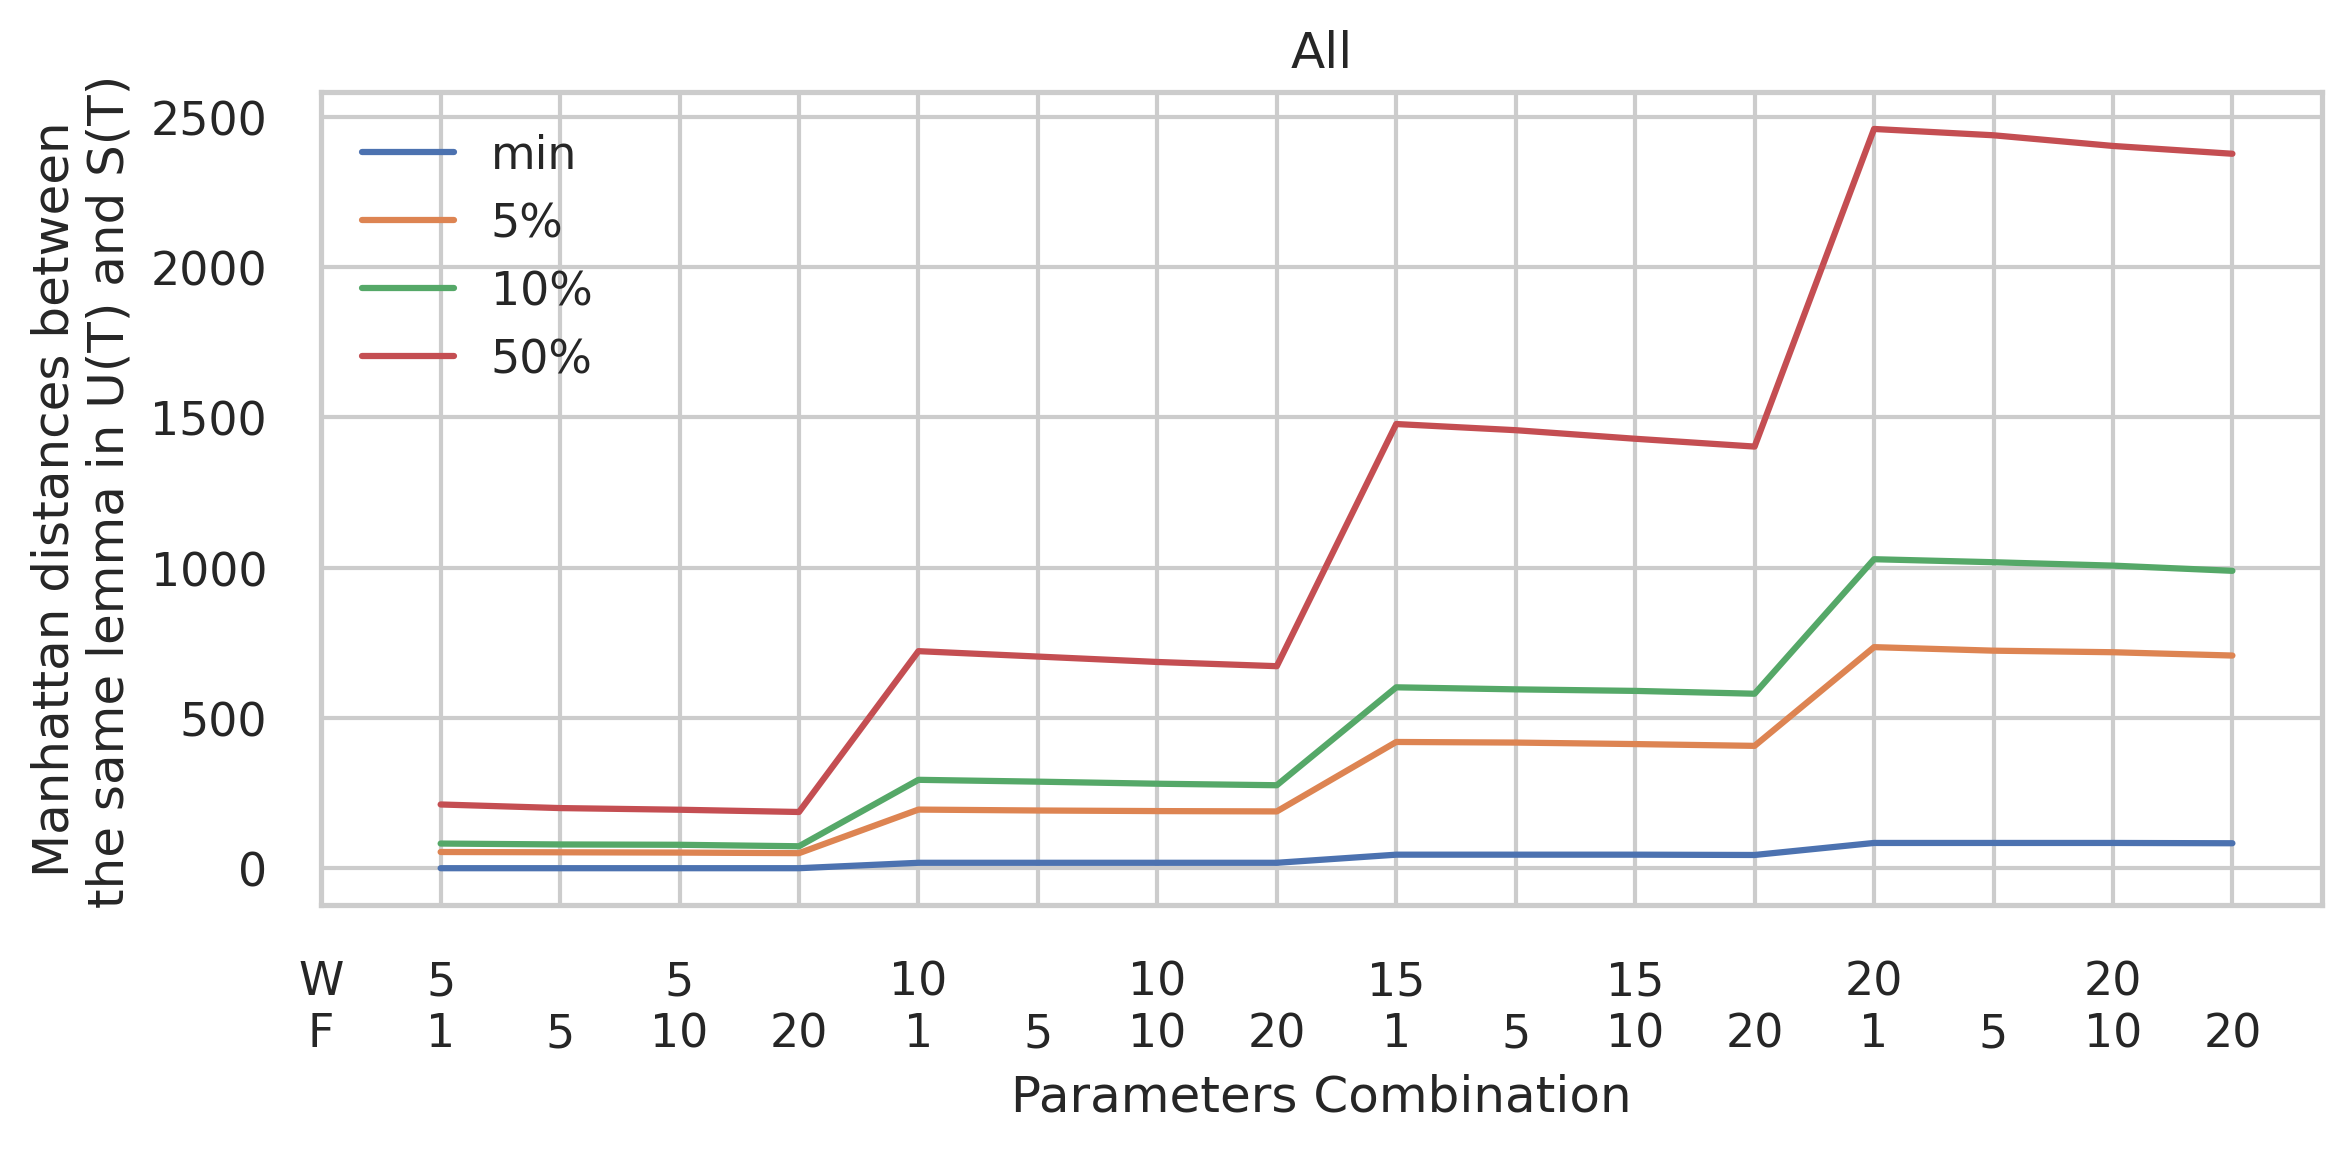
\includegraphics[width=.8\linewidth]{figures/chap1/part2/manhattan_All.png}
    \caption{Variation des percentiles (5, 10, 50) et de la valeur minimale des distances de Manhattan entre les vecteurs de chaque pivot dans $U(T)$ et $S(T)$ en fonction des valeurs de $W,F$. Résultat pour les mots les plus fréquents (\textit{Top 1000}) sur les trois sous-corpus (\textit{Martial et Priapea} en haut à gauche, \textit{ATU} en haut à droite, \textit{All} en bas).}
    \label{fig:chap1:noise:manhattan}
\end{figure}

On distingue nettement trois effets dans les résultats (\textit{cf.} figure \ref{fig:chap1:noise:manhattan}):
\begin{itemize}
    \item Quelle que soit la fenêtre $W$, le seuil $F$ a un effet très limité. Ce filtrage croît -- même minimalement -- en même temps que sa valeur: plus il est grand, plus il réduit la distance mesurée.
    \item Le changement de la taille de la fenêtre $W$ a un impact important sur les distances intervecteur, ce qui est attendu: plus le contexte relevé est grand, plus il est probable que ce contexte \enquote{pioche} dans des unités voisines, mais indépendantes.
    \item Tous les sous-corpus sont touchés, mais tous les mots ne sont pas touchés autant. À partir du corpus \textit{ATU}, certains mots sont très peu touchés voir indemnes de toute contamination. Cependant, on aperçoit dès le percentile 5\% des variations de plus en plus importantes en fonction de $W$.
\end{itemize}

Du point de vue de la collecte brute donc, il est clair qu'une différence existe entre $S(T)$ et $U(T)$.

\paragraph{Sur les classes}
\label{sub:major-co-occurrences}

Sur la base de cette première observation, nous voulons évaluer ce que ce bruit peut faire à des sélections de caractéristiques plus avancées. Chez Guerreau et Perreaux, le coefficient de Dice est utilisé pour trouver des termes \textit{affiliés} aux termes qu'ils veulent étudier pour les placer dans des réseaux plus grands. En appliquant ce coefficient et en sélectionnant les termes les plus proches, on peut alors comparer les co-occurrents majeurs sélectionnés ($M$) dans $U(T)$ et $S(T)$. Compte tenu des différences de distances constatées ci-dessus, on cherche donc à vérifier si ces dernières sont à même d'être gommées par une normalisation. 

\begin{figure}[h]
    \centering
    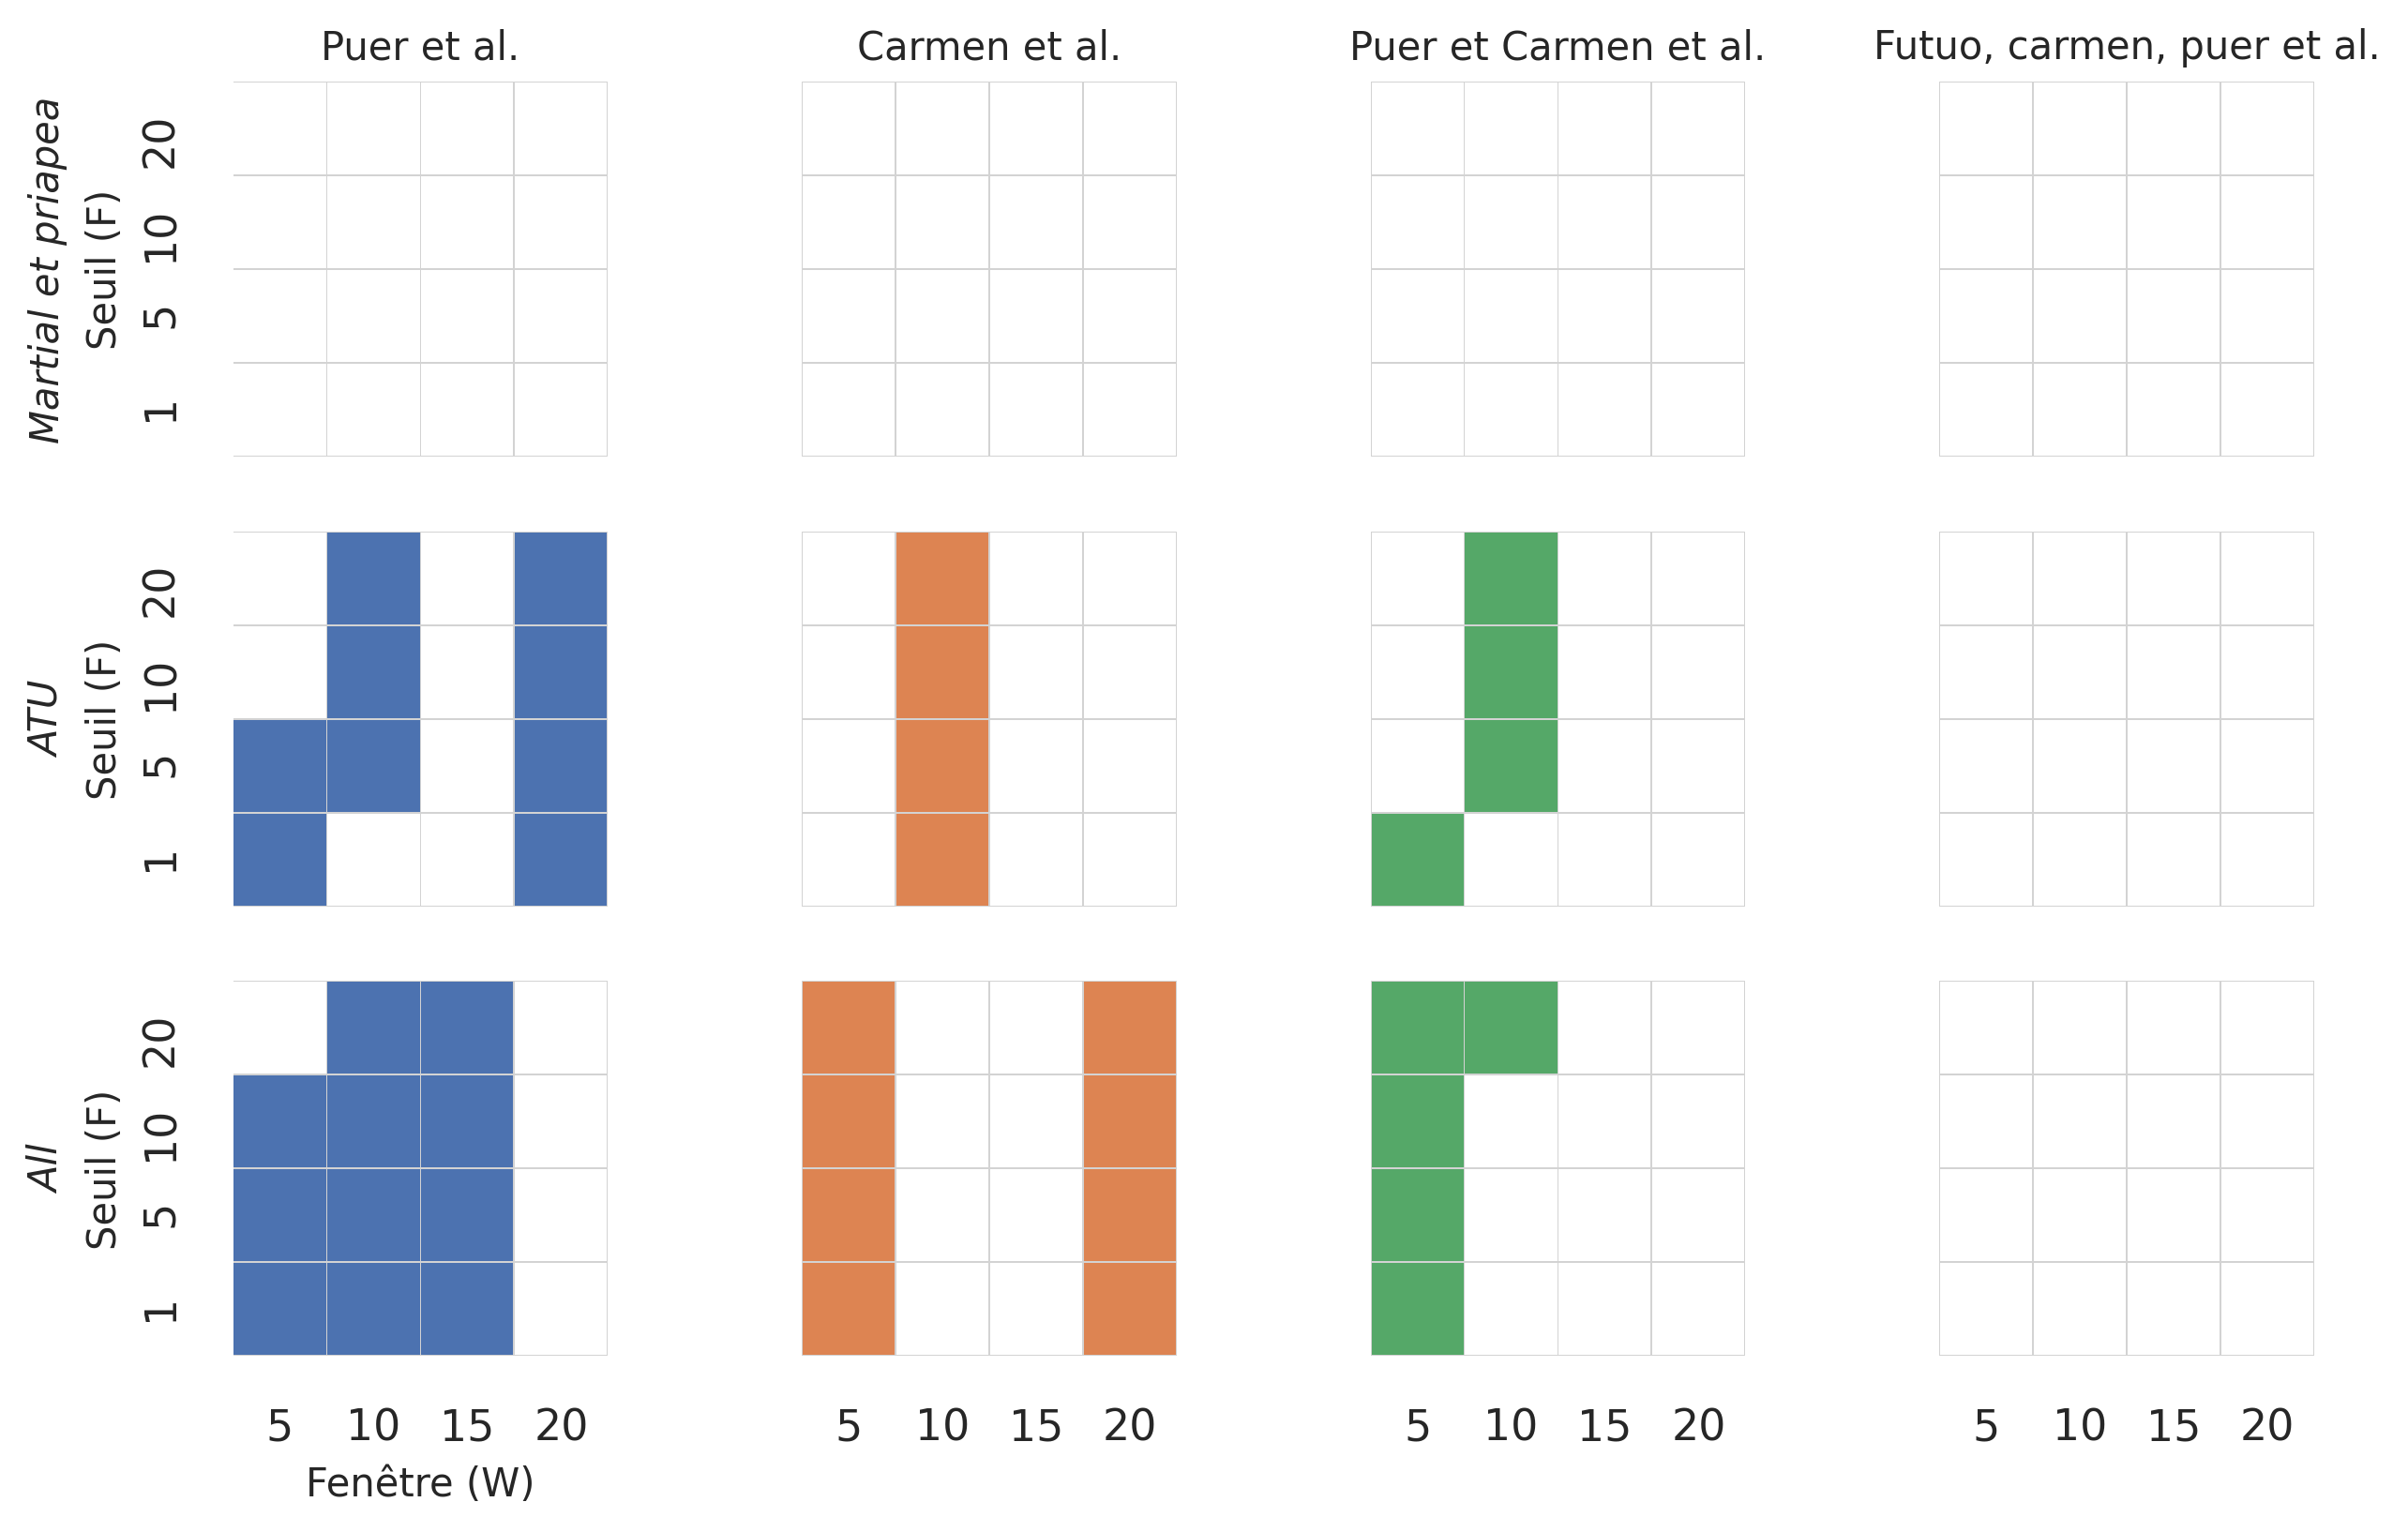
\includegraphics[width=.95\linewidth]{figures/chap1/part2/classes_binary.png}
    \caption{Matrice binaire de $M_{S(T)} = M_{U(T)}$ : les cellules colorées signifient que l'analyse des deux versions du corpus avec les mêmes paramètres a donné lieu aux mêmes co-occurrences majeures.}
    \label{fig:chap1:noise:matrix_classes}
\end{figure}


 Nous quantifions d'abord cet effet par une approche binaire, c'est-à-dire que nous vérifions que $M_{S(T)}$ et $M_{U(T)}$ sont strictement égaux. Toute situation où $M_{U(T)} \neq M_{S(T)}$ est une autre preuve que l'absence de segmentation a un impact. Or, seuls 21,35\% (41/192) des expériences et combinaisons de paramètres et données étudiées (Mots, Fenêtre, Seuil, Corpus) produisent une sélection de co-occurrents majeurs parfaitement égaux pour les deux versions de $T$, avec des résultats variables selon le groupe de mots et le corpus (\textit{cf.} Figure~\ref{fig:chap1:noise:matrix_classes}) :
 
% [2/1/22] RÉDACTION REPRENDRE ICI

 \begin{itemize}
    \item Le groupe de mots ``\textit{Futuo et al.}'' ne donne jamais lieu à des $M$ identiques entre $S(T)$ et $U(T)$. Il s'agit du seul groupe de mots ne formant jamais d'identité entre les deux versions du corpus: il est caractérisé par des fréquences plus basses que les autres groupes -- à travers \textit{irrumo} par exemple -- et est donc plus touché par le bruit dû à l'absence de segmentation.
    \item Tout comme ``\textit{Futuo et al.}'', le corpus \textit{Martial \& Priapea} -- le plus petit et le plus riche en ATU -- est fortement affecté par la différence de traitement des textes: aucune analyse ne produit de $M$ identiques, le bruit n'est pas atténué par la normalisation.
    \item Le groupe ``Puer et al.'' atteint majoritairement une égalité de résultat sur le corpus \textit{ATU Corpus} (neuf combinaisons sur seize), mais cette attitude est inconstante en regard de $W$ et $F$. Cela plaide simplement en faveur d'une segmentation des corpus (S)ATU riches comme préalable à une analyse similaire à celle que nous menons ici. La fréquence ``plutôt faible'' de \textit{libellus}~(546) dans le \textit{Carmen et al.} et le \textit{Puer et Carmen et al.} pourrait être responsable d'une partie de l'instabilité, bien qu'elle soit bien au-dessus de la fréquence de l'ensemble des termes  de la sexualité.
    \item La taille des corpus lisse le bruit des caractéristiques, car le corpus \textit{All} affiche une plus grande stabilité entre $M_{S(T)}$ et $M_{U(T)}$, en particulier pour \textit{Puer et al.}, mais les $M$ restent plus souvent inégaux qu'égaux.
    \item Le seuil de fréquence des co-occurrences $F$ a un impact très faible sur les co-occurrences majeures, comme vu précédemment pour \textit{Top 1000}, tandis que la fenêtre affecte irrégulièrement les ensembles de mots. À titre d'exemple, $W=15$ ne produit jamais de résultats identiques entre $S(T)$ et $U(T)$ pour la combinaison \textit{Carmen et al. }~+~\textit{All} (orange, en bas), mais elle le fait pour  \textit{Puer et al.} (bleu, en bas); au contraire, $W=15$ échoue sur \textit{Puer et al.}~+~\textit{ATU}. Cette instabilité de l'impact de $W$ plaide également en faveur de l'utilisation de (S)ATU lors d'une telle analyse.
\end{itemize}

\begin{figure}[h]
    \begin{minipage}[t]{.55\linewidth}
        \centering
        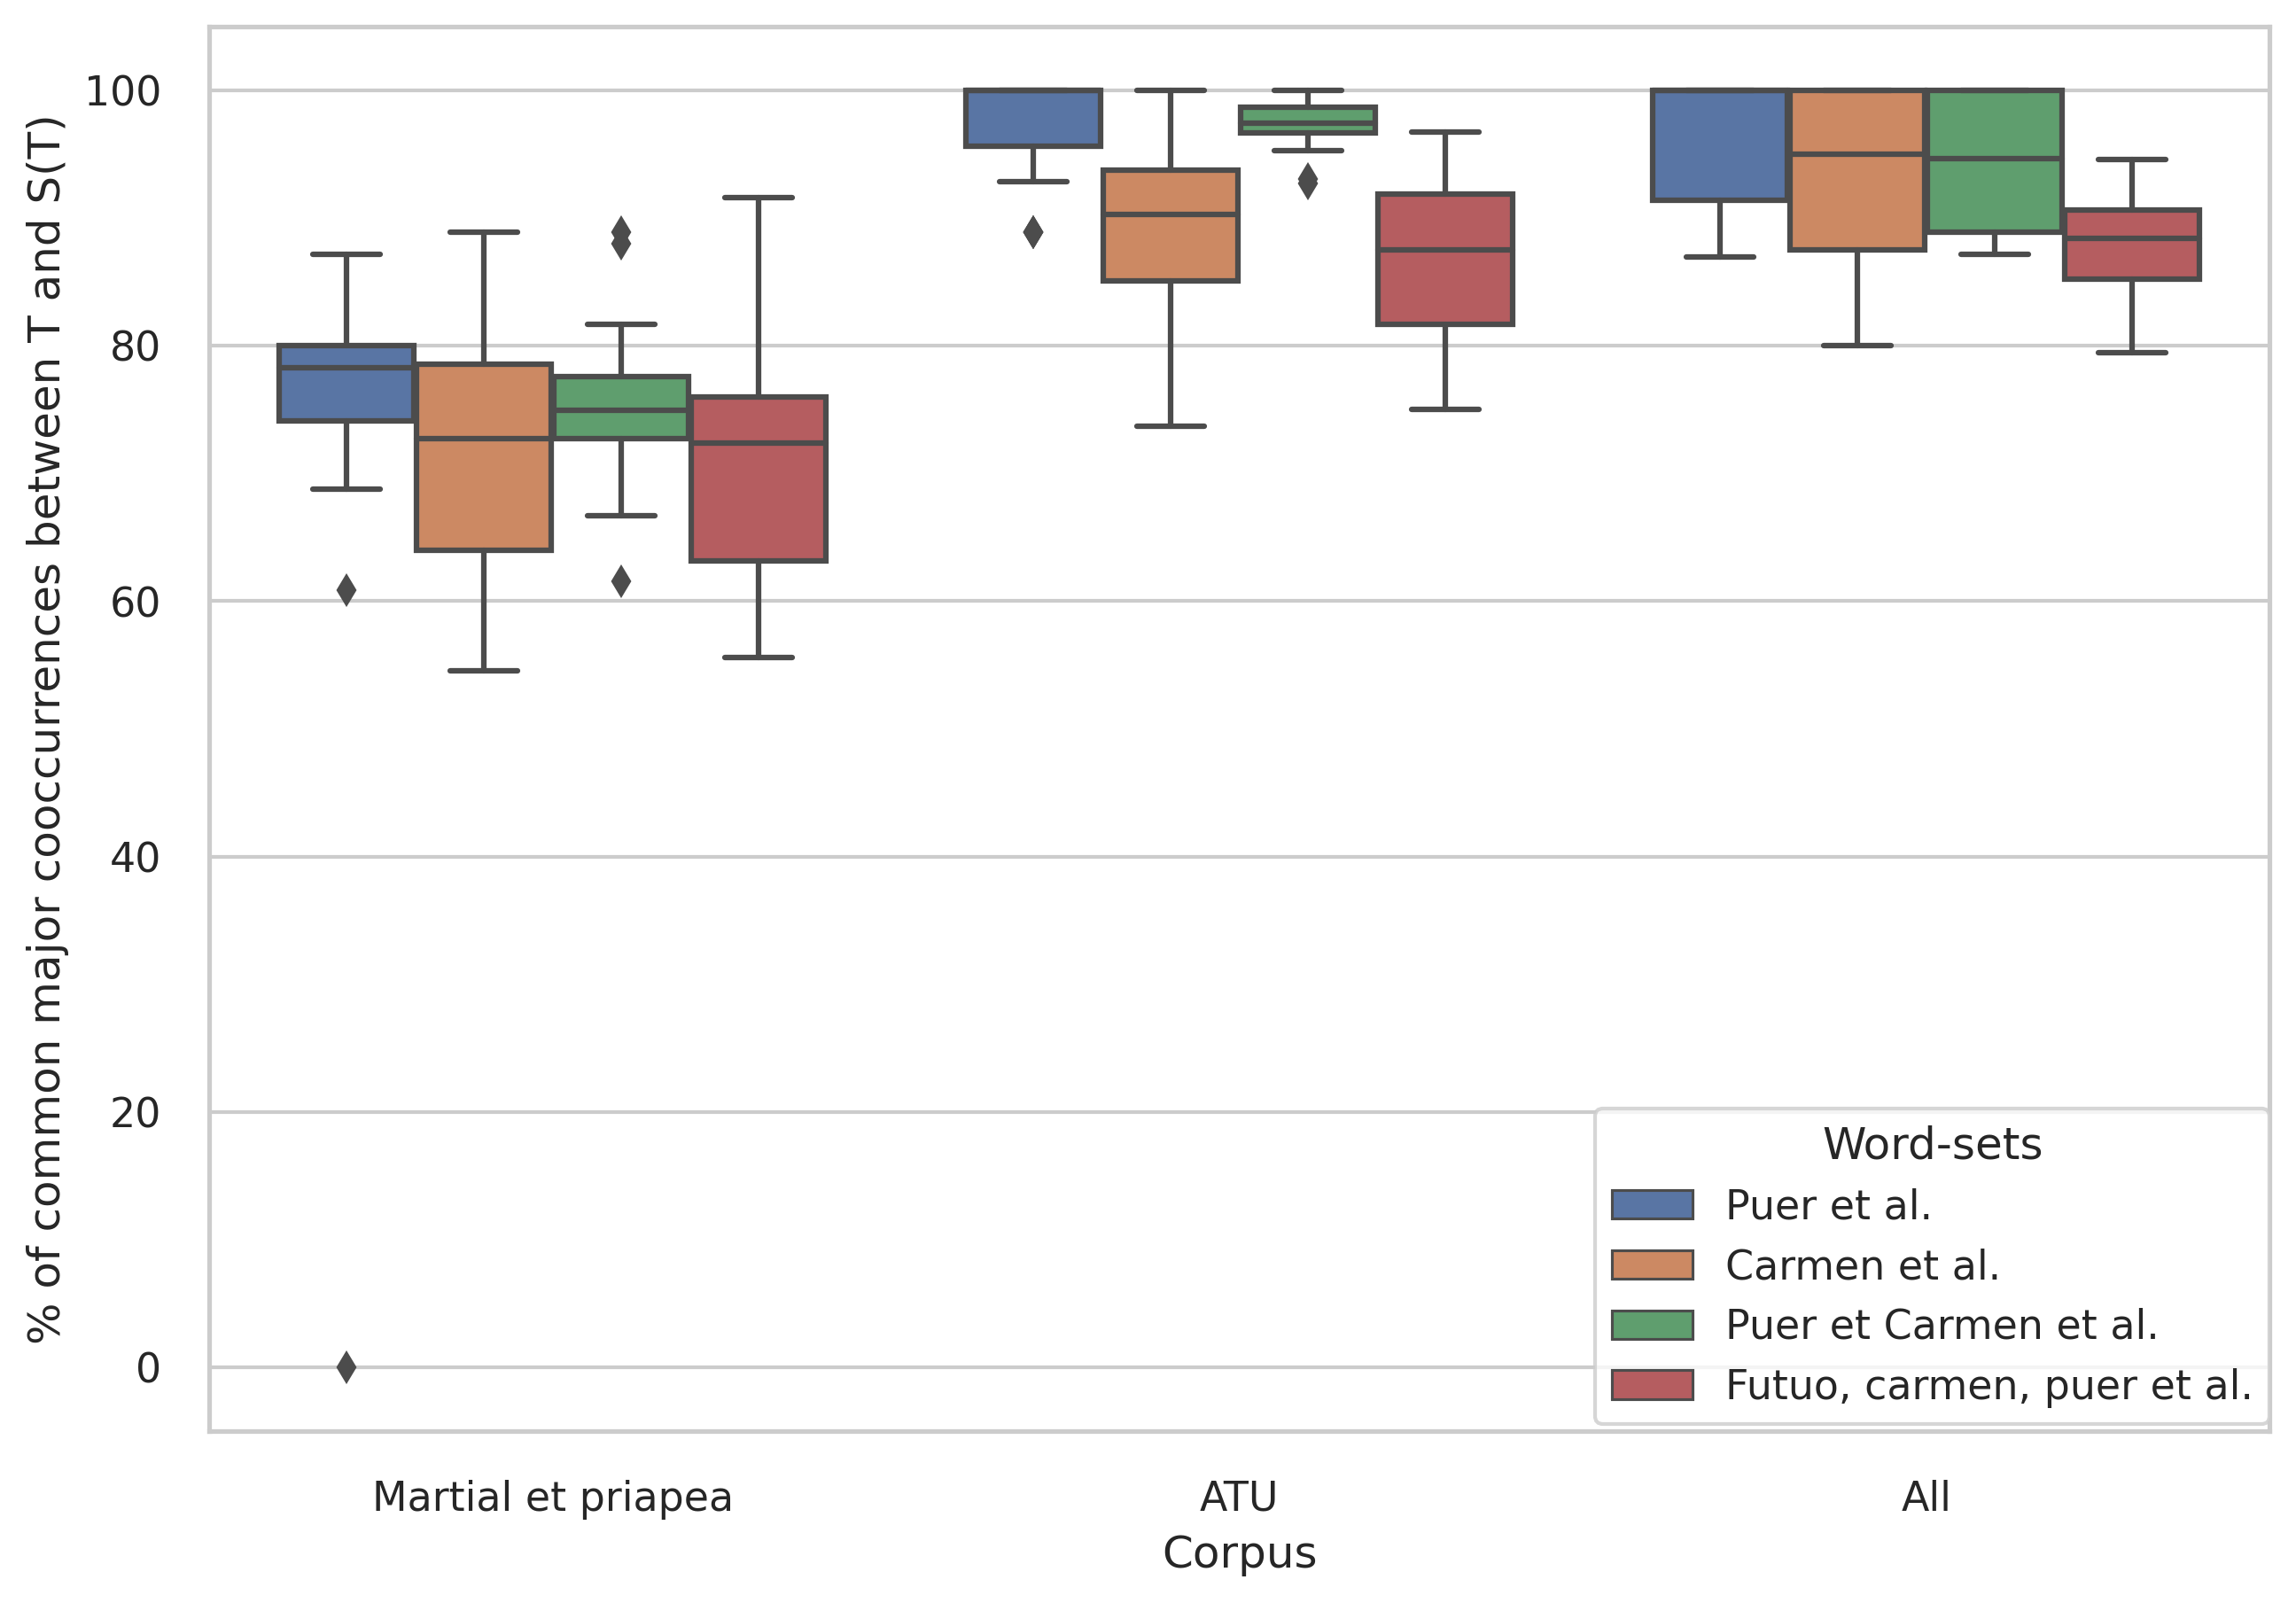
\includegraphics[width=1\linewidth]{figures/chap1/part2/classes_percent.png}
        \caption{Dispersion du \textit{taux de similarité} entre $M_{S(T)}$ et $M_{U(T)}$ pour chaque combinaison de corpus et de mots. Pour \textit{Puer et al.} sur \textit{Martial et Priapea}, les principales co-occurrences ont une similarité médiane inférieure à 80\% sur les 16 combinaisons de $W,F$. Les valeurs aberrantes ne sont pas affichées.}
        \label{fig:classes_de_violon}
    \end{minipage}%
    \hfill%
    \begin{minipage}[t]{.43\linewidth}
        \centering
        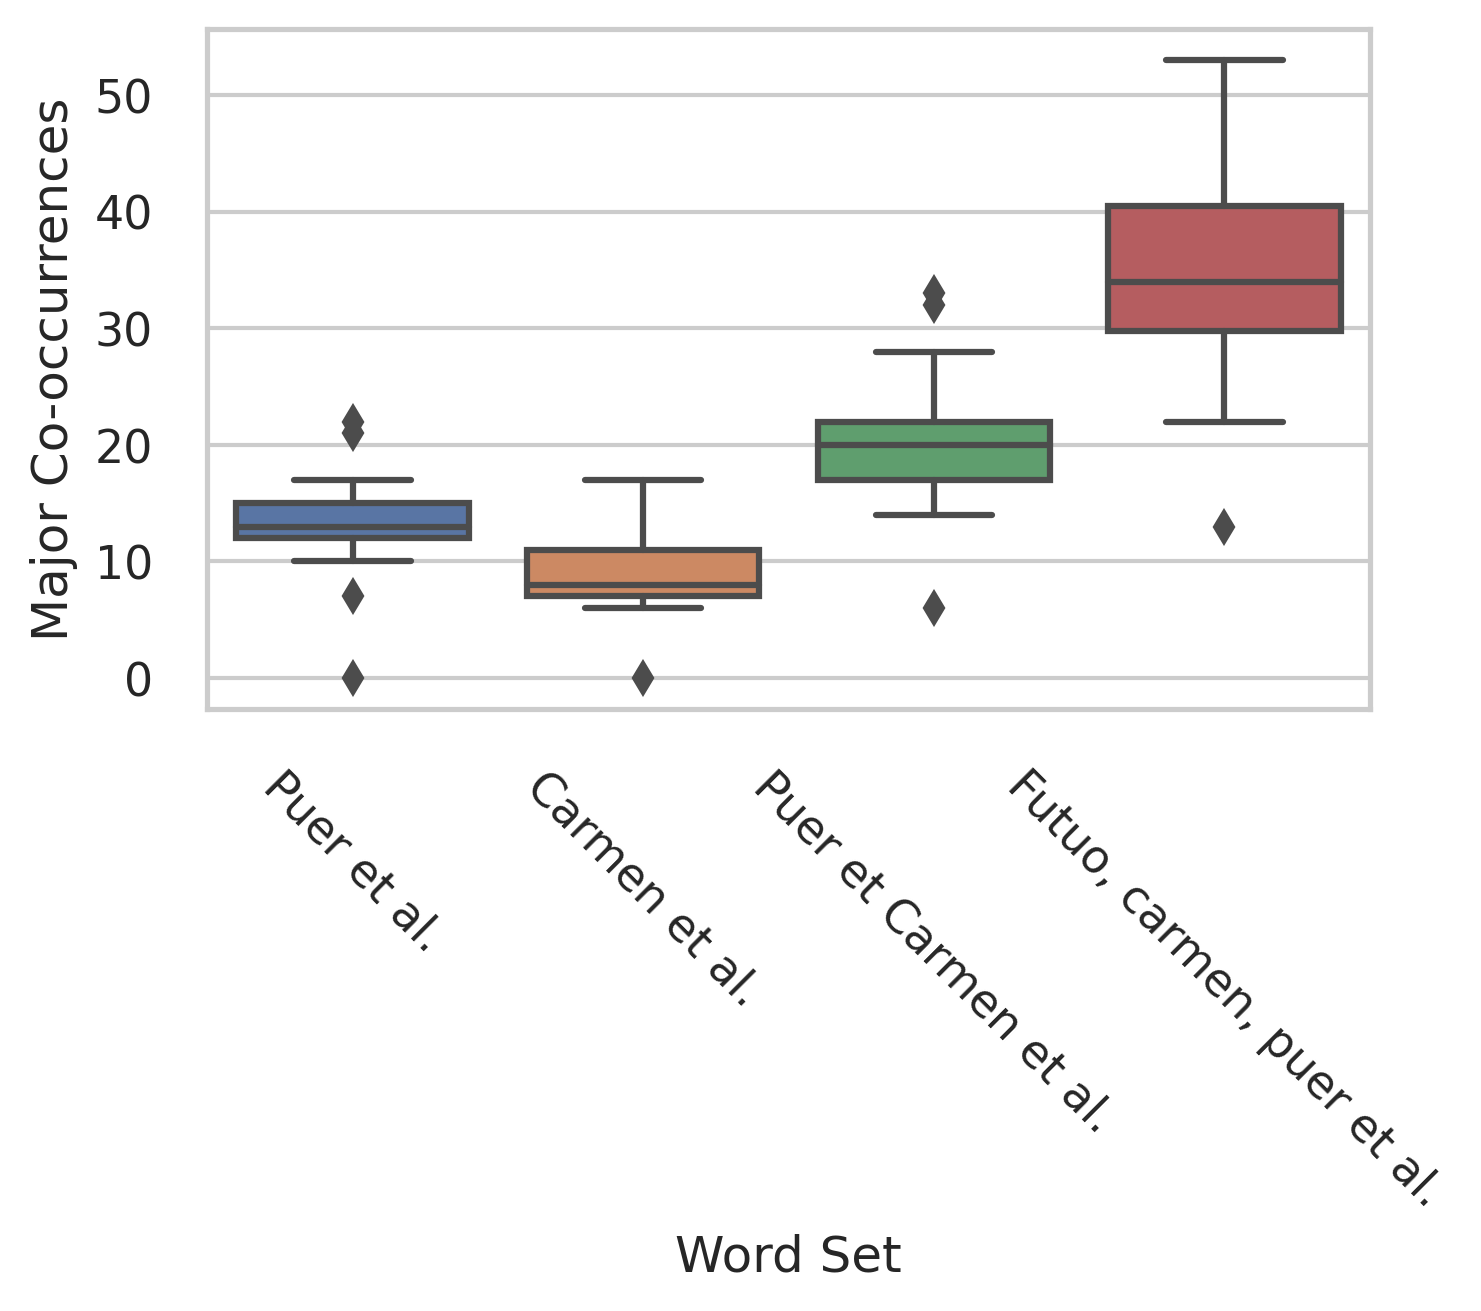
\includegraphics[width=\linewidth]{figures/chap1/part2/major_count.png}
        \caption{Nombre de co-occurrences majeures par ensemble de mots}
        \label{fig:chap1:noise:major_count}
    \end{minipage}
\end{figure}



Cette approche binaire reste limitée et ne donne pas une idée complète de l'impact de l'absence de la segmentation: est-ce un seul mot ou la moitié des composants de $M$ qui diffère entre les deux versions de chaque corpus ? Pour répondre à cette question, nous proposons d'évaluer le \textit{taux de similarité} en fonction des deux ensembles $M$ de co-occurrences majeures, calculés :

\begin{equation*}
    1 - \frac{%
        \left | M_{S(T)} - M_{U(T)} \right | + \left | M_{U(T)} - M_{S(T)} \right |%
    }{%
       \left | M_{S(T)} + M_{U(T)} \right |%
    }
\end{equation*}

À quelques exceptions près sur \textit{Martial \& Priapea} et \textit{Corpus ATU}, le taux de similarité est généralement supérieur à 60\% pour le plus petit corpus, 80\% pour les deux autres \footnote{Voir tableau annexe \ref{tab:anx:noise:capitains:ratio_classes}} alors même que la taille médiane de $M$ se situe entre 8 (\textit{Carmen et al. }) et 34 (\textit{Futuo, carmen, puer et al.)} (\textit{cf.} figure \ref{fig:chap1:noise:major_count}). Quelle que soit la taille du corpus et de l'ensemble de mots, le taux de similarité est globalement élevé: les grands corpus montrent une certaine résistance au bruit, comme nous l'avons vu dans les analyses binaires, et les petits corpus ou groupes de mots à faible fréquence connaissent des variations plus grandes entre $U(T)$ et $S(T)$.

Globalement, les deux métriques montrent cependant un effet incontestable sur la sélection des co-occurrences majeures. Même si la taille du corpus atténue cet effet, comme le montrent les résultats de \textit{All} par rapport aux autres, elle ne garantit pas l'égalité des résultats entre $S(T)$ et $U(T)$, comme le montrent $W=20$ pour \textit{Puer et al.} ou $W=10$ et $W=15$ pour \textit{Carmen et al.}. La manipulation minutieuse des (S)ATU dans des corpus relativement petits ($\leq20M$ tokens) doit être une étape importante pour renforcer toute analyse statistique sémantique, car on ne saurait garantir que les résultats ne soient pas fortement contaminés par de faux co-occurrents.


\paragraph{Sur les caractéristiques}
\label{sub:clustering}

Sur la base de la normalisation de la matrice des co-occurrents des pivots et de $M$, nous voulons identifier si des algorithmes plus avancés étaient aussi sujets à des variations avec cette entrée normalisée. Pour chaque combinaison de $W,F$, on cherche à savoir si les \textit{clusters} $K$ produits par les outils précédemment cités forment une identité de sorte que $K_{S(T)} = K_{U(T)}$ (\textit{cf.} figure \ref{fig:chap1:noise:clusters_rates}). Étant donnés les résultats précédents, impliquant une inégalité courante des $M$, et afin de former avec les pivots un $C$ stable, on s'assure d'abord de filtrer les $M$ de sorte que $C = \text{Pivots} + M_{S(T)} \cap M_{U(T)}$ avant de clusteriser. On ne cherche pas à optimiser $k$, le nombre de \textit{clusters}: il doit simplement respecter la condition $\frac{\left | C \right |}{k} \geq 2$ afin d'avoir au moins deux mots par \textit{cluster} cherché.

\begin{figure*}[ht]
    \centering
    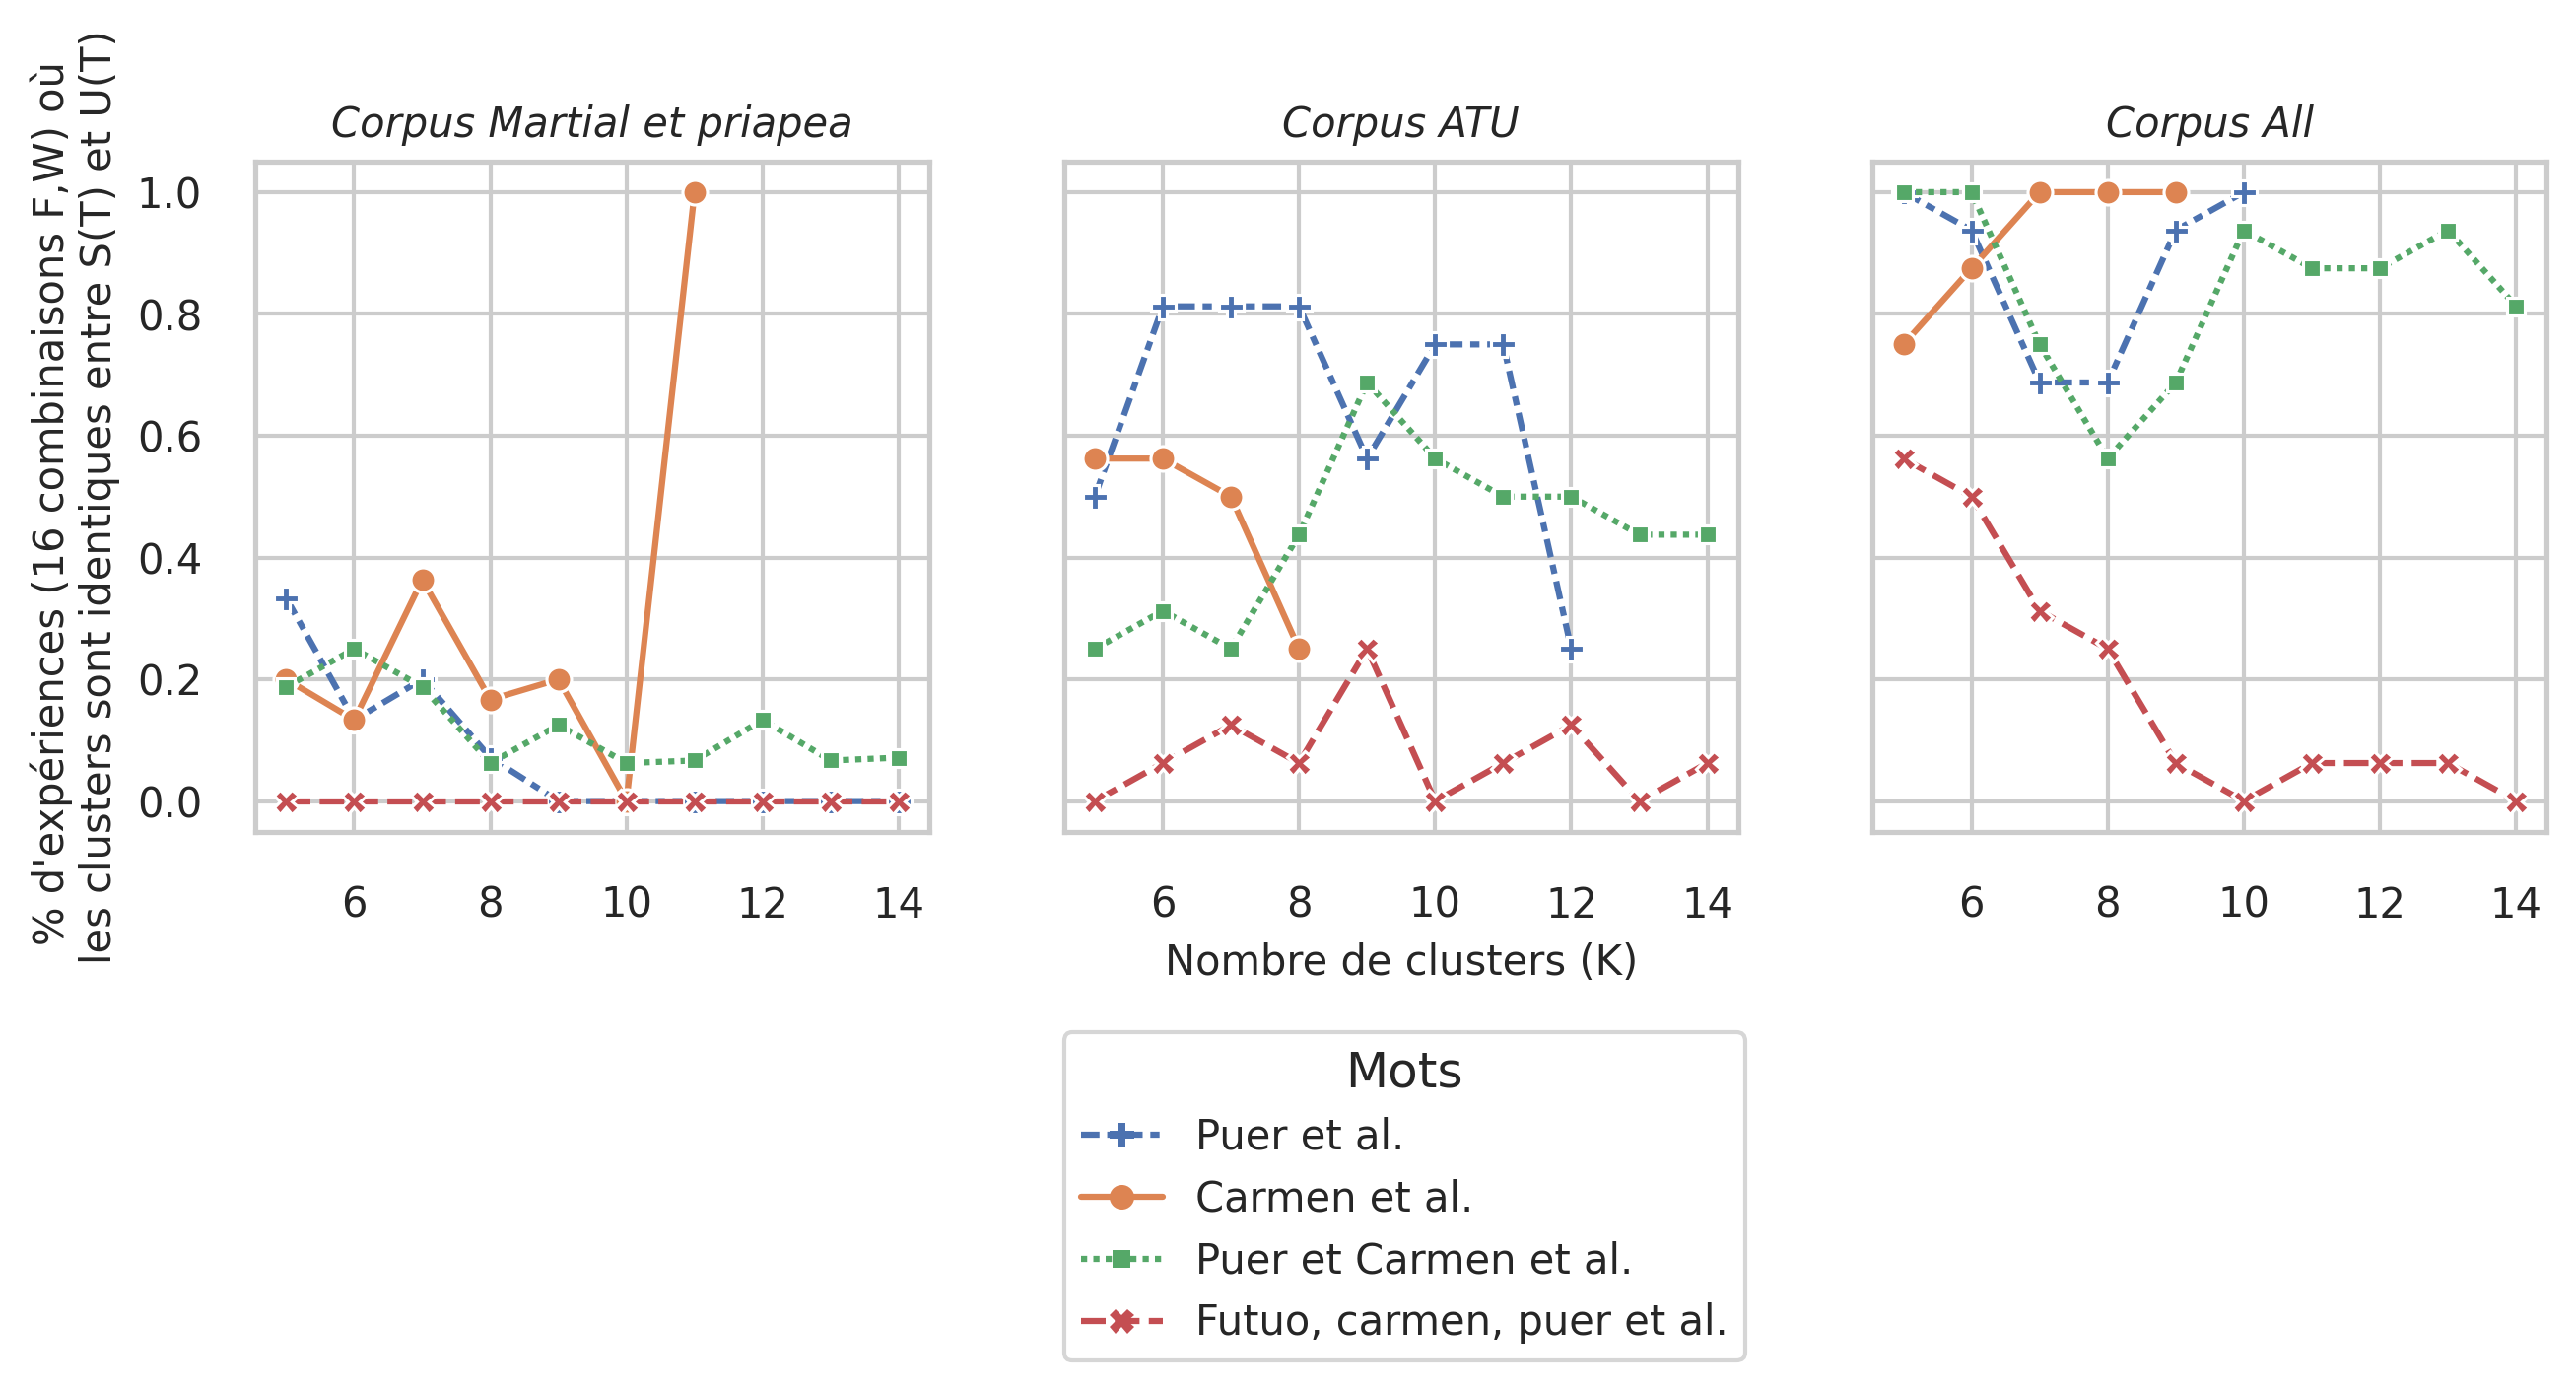
\includegraphics[width=1\linewidth]{figures/chap1/part2/cluster_binary_rates.png}
    \caption{Ratio des expériences où $K_{S(T)} = K_{U(T)}$ étant donné le nombre de \textit{clusters} $k$ et les matrices résultats de chaque expérience variant sur $W,F$ pour chaque corpus et ensemble de mots.}
    \label{fig:chap1:noise:clusters_rates}
\end{figure*}


Dans ce contexte, les caractéristiques ont un impact qui va au-delà de la simple sélection de classes, notamment pour nos deux premiers corpus. Sur \textit{Martial \& Priapea}, quel que soit le groupe de mots étudié, seuls \textit{Carmen et al.} avec $k=11$, parmi l'ensemble des analyses (variant sur $F,W$), produit les mêmes \textit{clusters} pour $S(T)$ et $U(T)$. Aucune des clusterisations sur le corpus \textit{ATU} ne produit le même résultat sur l'ensemble des variations $F,W$ d'une version à l'autre du corpus. En général, moins de 40\% des combinaisons $F,W$ produisent les mêmes clusters pour $C$ sur le plus petit corpus. Comme pour l'analyse des classes, ce chiffre augmente avec la taille du corpus, qui atténue donc en partie l'effet de $S$ sur $T$. Avec 80\% de combinaisons $F,W$ à clusterisations similaires maximums pour \textit{ATU} et 100\% pour \textit{All}. Cependant, cet effet est encore instable et imprévisible: alors que \textit{Puer et al.} atteint 100\% d'expériences ($F,W$) égales dans leur clusterisation entre $S(T)$ et $U(T)$ avec $K=5$ et $K=10$, il tombe à 70\% pour $K=7$ et $K=8$. Cette instabilité s'ajoute au fait que les données ont déjà été \enquote{manipulées} en réduisant les $M$ à un set commun $C$.

\subsubsection{Conclusion de l'expérience}

% Rework CONCLUSION

En 1957, J. R. Firth a utilisé le terme de \textit{company}. Dans notre expérience, il devient contexte pour la lecture humaine et fenêtre pour l'ordinateur. Mais ce que l'auteur entendait est beaucoup plus précis que d'avoir deux mots qui se suivent dans un fichier: il est fort peu probable que, face à deux articles de presse sur une même page, J. R. Firth eût accepté de dire que le dernier mot d'un article est \textit{company} du premier mot de l'article suivant. La réponse devrait être claire pour n'importe quel linguiste ou philologue, et pourtant, les textes et les œuvres composites ont été traités de cette manière par des études en humanités numériques ou en TAL\footnote{\textit{cf.} \textcite{kontges_measuring_2020} par exemple.}. 

Dans cette expérience, nous avons évalué l'impact de la non-prise en compte de la structuration des textes. Bien que le fait de travailler avec des statistiques sur des corpus aussi petits exige par nature de la prudence, nous avons démontré que le fait de traiter les œuvres numérisées comme des unités \textit{de facto} homogènes et indissociables plutôt que comme un patchwork de plus petites unités modifie les résultats de l'analyse distributionnelle avec des corpus comptant jusqu'à une vingtaine de millions de mots. Dans nos expériences, seules quelques combinaisons des différents paramètres communs à ces applications (taille de la fenêtre, seuil de fréquence, taille du cluster) ont donné des résultats cohérents entre un corpus de textes édités ($S(T)$) et une version brute de celui-ci ($U(T)$). Avec des mots fréquents dans tout le corpus, avec une petite fenêtre ($W=5$) et de grands corpus, l'effet du bruit est atténué. En revanche, si ces mots sont plus fréquents dans des œuvres très segmentées comme la compilation de poèmes, la taille du corpus global aura moins d'impact sur la question. 

Ces résultats justifient la nécessité de textes enrichis de métadonnées qui permettent un post-traitement tel que celui permis par CapiTainS et l'environnement TEI XML original. Ils plaident définitivement pour l'utilisation de déclarations de segmentation avec des métadonnées telles que \texttt{CiteStructure}\footcite{cayless_introducing_2021} afin de rendre ces corpus utilisables par des machines. Certes, ils limitent la taille du corpus et ne permettent pas nécessairement d'utiliser toute la richesse des corpus en friche présentés auparavant: mais ils montrent sans appel qu'il n'existe pas de combinaison de paramètres nous assurant une protection complète des contaminations.


\section{Constitution d’un corpus sur l’expression de la sexualité} 

Disposant d'un meta-corpus de près de vingt millions de mots en latin, il est désormais possible de passer à la compilation d'un exemplier. Le \textit{Wiktionnaire} définit un exemplier comme \enquote{une liste d’exemples [Définition 1] ou de citations [Définition 2] à but pédagogique\footcite{noauthor_exemplier_2019}}, pour E. Crespo, il s'agit de la \enquote{feuille
d’exemples sur laquelle un intervenant appuie son exposé oral}\footcite{crespo2011pour}. Sur la base de ces usages, il est important alors de développer une explication de ce qui est entendu par \enquote{exemplier numérique}. Un exemplier numérique partage avec le corpus numérique l'idée d'une collection de textes dans des formats exploitables par la machine, tandis qu'il retient de l'exemplier papier (1) le caractère fragmentaire -- il ne s'agit que de citations, d'extraits --, (2) sa cohérence thématique, (3) sa visée pédagogique. 

Or, pour aborder l'histoire de la sexualité ou son lexique, ce genre de compilations de source semble important pour un renouvellement de la lexicographie ou de l'historiographie, à l'image de ce qui est fait en histoire des femmes avec des projets comme Eurykleia\footcite{noauthor_eurykleia_nodate}. Il faut mettre à disposition un exemplier numérique, requêtable et manipulable, pour mieux cerner la richesse linguistique du latin sur ce thème, tout comme les réalités qu'il recouvre. Les éléments de notre exemplier ne sont que les préliminaires d'un travail de longue haleine, qui viserait à fournir -- dans un objectif pédagogique -- à quiconque les ressources nécessaires pour embrasser le sujet dans sa diversité.

Cette visée pédagogique ne concerne pas que les étudiants ou chercheurs qui souhaiteraient découvrir le lexique spécifique à la sexualité mais aussi les tournures et expressions \textit{ad hoc} ou imagées parcourant la littérature latine. Il s'agit aussi, dans un premier temps, d'enseigner à la machine comment reconnaître un passage, une phrase ou un ensemble syntaxique cohérent, qui présenterait l'isotopie de la sexualité.

En premier lieu, nous présenterons une courte histoire de la lexicographie de la sexualité et de l'historiographie de ce sujet, en appuyant tout particulièrement sur la source presque unique de notre exemplier numérique de la sexualité en latin, à savoir le \textit{Latin Sexual Vocabulary} de J. N. Adams\footcite{adams}. Dans un second temps, nous discuterons de la production de l'exemplier numérique, de ses principes aux méthodes de compilations. Enfin, nous présenterons comme nous l'avions fait pour le méta-corpus ses caractéristiques statistiques.

\subsection{\textit{Latin Sexual Vocabulary} de J. N. Adams: une source unique ?}

\subsubsection{(D)Écrire le lexique latin de la sexualité: une histoire}

\begin{quote}[Avant-Propos]{Michel Dubuisson, \textit{Lasciva Venus: petit guide de l'amour latin}}
    \enquote{``Le latin dans les mots brave l'honnêteté'' disait le bon Boileau. Il est vrai que la littérature latine peut passer, du moins aux yeux de ceux qui l'ont fréquentée en dehors des classes, pour l'une des plus pornographiques qui soit.}
\end{quote}

Dans son ouvrage grand public, \textit{Lasciva Venus: petit guide de l'amour latin}, Michel Dubuisson, professeur de littérature latine, ne ménage pas les attentes de son lecteur dès les premières pages. La littérature latine serait donc \enquote{pornographique}. Mais cette catégorie, moderne, sous-entend aussi de la bouche de l'auteur une graduation. Il y aurait ainsi:
\begin{itemize}
    \item une littérature pornographique et donc \enquote{appelant un chat un chat -- en l'occurrence une chatte (\textit{cunnus})} comme le dit si bien le même auteur quelques lignes plus loin;
    \item une expression plus nuancée que l'on pourrait qualifier d'érotique, parlant d'actes sexuels et de ce qui les entoure sans être aussi cru que le discours pornographique;
    \item une manière d'aborder le sujet de manière neutre, faisant émerger des discours sur les corps, médicalisés ou moralisateurs.
\end{itemize}

L'histoire de ces discours et de leur lexique ont une histoire particulièrement courte: d'un sujet peu abordé au XIX\textsuperscript{e} puis au début du XX\textsuperscript{e}, si ce n'est sous un aspect religieux, son étude a été totalement renouvelée depuis cinquante ans. Nous nous proposons de revenir sur trois jalons de cette histoire, de manière thématico-chronologique: d'abord, à travers les rares publications lexicographiques du XIX\textsuperscript{e}, puis en nous intéressant au renouvellement de l'historiographie de la sexualité, en terminant par celui de la lexicographie aux alentours des années 1970 et 1980.

\paragraph{Le XIX\textsuperscript{e} siècle, premiers glossaires}

Le début du XIX\textsuperscript{e} siècle connaît une formidable double production sur ce sujet et démarre une tradition bi-centenaire des lexiques et exempliers de la sexualité en latin. En 1822, F.~K.~Forberg, conservateur de bibliothèque, publie à Cobourg (Bavière) l'édition de poèmes d'un auteur italien du XV\textsuperscript{e} siècle, Antonio Beccadelli (1394--1471)\footcite{beccadelli_antonii_1824}. Mais la particularité de cette édition est qu'elle est augmentée de tout un commentaire, le \textit{De figuris Veneris} (fr. \textit{Des positions de Vénus}), sur les positions et pratiques sexuelles diverses des Romains, appuyé sur des exemples tirés de la littérature latine. Bien plus tard, en 1882, ce traité, rebaptisé \textit{Manuel d'érotologie classique} pour l'occasion\footcite{forberg_manuel_1882}, est traduit par Alcide Bonneau (cette édition sera traduite en anglais en 1884)\footcite{parra1997figuris}. Une autre édition bilingue latin-français est publiée par Henri Daragon sous le titre \textit{De Figuris Veneris (Des formes du baiser)}\footcite{forberg_f_1907} dans la collection des Enfers de la Bibliothèque nationale de France. Le texte en lui-même est constitué, dans son édition originale, de 8 chapitres thématiques (hors introduction): de la \textit{fututio} (pénétration vaginale, 39 pages), de la \textit{paedicatio} (pénétration anale, 23 pages), de l'\textit{irrumatio} (sexe oral lié au pénis, 27 pages), de la \textit{masturbatio} (17 pages), du \textit{cunnilingus} (23 pages), des tribades (homosexuelles femmes, 24 pages), du \textit{coitum cum brutis} (zoophilie, 3 pages), et des \textit{spintria} (positions sexuelles impliquant dans ce contexte plus de deux partenaires, 5 pages). Les thématiques sont donc larges et diverses, comprenant à la fois les questions du sexe des partenaires -- manière anachronique de diviser les sexualités des anciens -- et les questions de ce qui est ou non pénétré. La première traduction française recompose le texte en six chapitres (on note les \enquote{nouveaux} chapitrages des cinquièmes et sixièmes parties \enquote{De la langue} et \enquote{Fantaisies}), là où celle de Daragon est plus fidèle.

%\begin{itemize}
%    \item Page 205-215, \textit{De Figuris Veneris}
%    \item Page 215-254, De Fututione
%    \item Page 254-277, De Paedicando
%    \item Page 277-304, De Irrumando
%    \item Page 304-321, De Masturbando
%    \item Page 322-345, De Cunnilingus
%    \item Page 345-369 , De Tribadibus
%    \item Page 369-372 , De coitu cum brutis.
%    \item Page 373-378 , De Spintriis ( des plans à trois ?: Les spintries sont une sorte d'innovateurs sexuels)
%    \item Page 379 (index des figures) Figurarum Veneris enumeratio,
%\end{itemize}

La deuxième production du XIX\textsuperscript{e} est le \textit{Glossarium eroticum linguae latinae} (\enquote{Glossaire érotique de la langue latine}) de Pierre-Emmanuel Pierrugues\footcite{pierrugues_glossarium_1826}, publié en 1826, soit quelques années à peine après les travaux de Forberg\footnote{Nous en proposons une version encodée en TEI: \textcite{Clerice_Lasciva_Roma_Lexical_2022}}. Contrairement à l'œuvre allemande, ce glossaire ne propose pas de classement thématique: c'est un lexique spécialisé, qui se lit comme un dictionnaire, et dont les entrées sont généralement fournies de références antiques ou tardo-antiques. La notion de sexualité y est aussi plus large, pour preuve les entrées \textit{Abortio}, \textit{Honor} et \textit{Ornatrices} (femme de chambre, \textit{habilleuse}). Il a la particularité d'avoir \textit{a priori} été copieusement plagié -- au sens moderne --, du moins d'après l'éditeur d'un \textit{Supplementum} en 1911\footcite{pierrugues_supplementum_1911}: il est en effet réimprimé en 1833 à Stuttgart sous le nom de \textit{Thesaurus eroticus linguae latinae} puis \textit{Der erotische Sprachschatz der Roemer} sous le nom de Carl Rambach. 

\begin{figure}
    \begin{minipage}{.45\linewidth}
        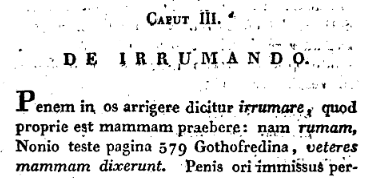
\includegraphics[width=\linewidth]{figures/chap1/part3/277_forberg.png}
        \caption{F.~K.~Forberg, page 277. Le lexique est abordé dans une description plus large des amours latines.}
    \end{minipage}%
    \hfill %
    \begin{minipage}{.45\linewidth}
        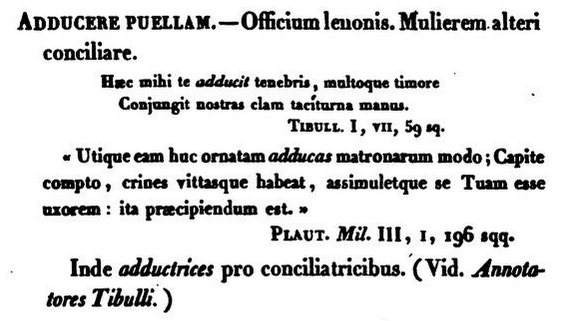
\includegraphics[width=\linewidth]{figures/chap1/part3/13_pierrugues.png}
        \caption{P.-E.~Pierrugues, page 13. Le lexique est écrit comme un dictionnaire unilingue.}
    \end{minipage}%
    \\
    \centering
    \begin{minipage}{.5\linewidth}
        \centering
        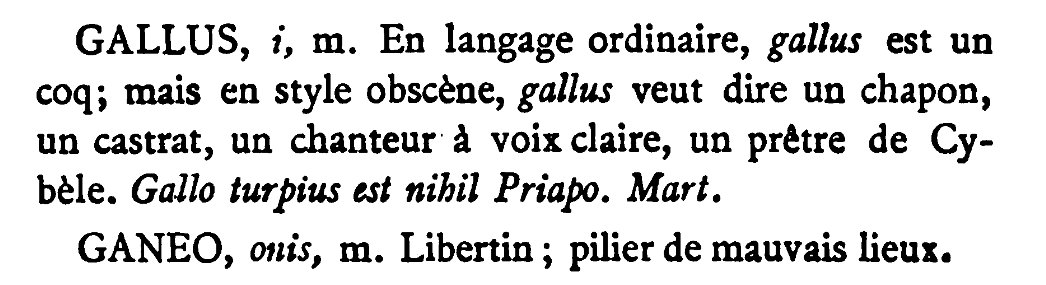
\includegraphics[width=\linewidth]{figures/chap1/part3/62_blondeau.png}
        \caption{N.~Blondeau, page 62. Traduction des termes latins avec explications, quelques citations non traduites.}
    \end{minipage}
    \caption{Exemples d'entrée dans les trois lexiques principaux du XIX\textsuperscript{e}.}
    \label{fig:chap1:exemples_dictionnaires}
\end{figure}

Ce supplément fait figurer des termes de l'ouvrage de Forberg, mais aussi d'un troisième ouvrage publié en 1882: le \textit{Dictionnaire érotique latin-français}\footcite{blondeau_dictionnaire_1885}. Le manuscrit d'origine serait de Nicolas Blondeau, dont on sait par l'éditeur qu'il aurait été avocat, censeur des livres et inspecteur de l'imprimerie à Trévoux en 1695. La preuve de son existence avant son édition provient \textit{du catalogue de la bibliothèque de feu M. Baron}\footcite[Chap. \textit{Belles-Lettres}, p.~2]{noauthor_catalogue_1788} sous l'index 4495, qui le qualifie d'autographe. Mais le texte imprimé en 1882 par Isidore Liseux, dont l'avant-propos nous fournit les éléments nécessaires pour suivre la trace et l'histoire du texte, est en fait un manuscrit à deux mains: le corps du texte est de la fin du XVIII\textsuperscript{e} et de la main de N.~Blondeau, tandis que les notes de bas de page sont issues des annotations d'un second scripteur, ancien possesseur du manuscrit, François Noël. Or, François Noël est bien connu d'Isidore Liseux: ancien enseignant à Louis-le-Grand, \enquote{prêtre défroqué de 1791}\footcite[p.~XVI]{blondeau_dictionnaire_1885}, il a commis l'édition d'un grand nombre de textes autour de la sexualité, de sélections d'épigrammes de Martial aux \textit{Priapées} en passant par quelques florilèges sur le même thème. L'impression du travail de F.~Noël était prévue, d'après les notes de Liseux, mais ne fut jamais mise en route. Cet ouvrage est d'ailleurs merveilleusement relié aux deux précédents, puisqu'il y est inclus un \textit{Essai sur la Langue Érotique} d'Alcide Bonneau, qualifié par son travail précédent \enquote{Traducteur du \textit{Manuel d'Érotologie} de Forberg}.


Les deux ouvrages de la décennie 1820 partagent la même particularité: ils sont entièrement en latin. De fait, il n'est donc pas possible pour l'ensemble des personnes capables de lire d'accéder à la substantifique moelle des travaux présentés, et cette débauche n'est donc disponible qu'aux latinistes, probablement perçus comme plus à même de se contrôler... Ce sont des ouvrages savants, l'un penche vers le manuel, l'autre vers le dictionnaire parfois moralisateur. Cette moralisation est complexe à évaluer, car si d'une part, il donne pour \textit{cunnum linguere} (lécher une chatte) \enquote{\textit{Foeditas Romanis usitatissima}} (\enquote{Horreur des plus répandues chez les Romains}), il appuie cette définition de vers parmi les plus crus chez Martial, issus de l'épigramme VII, 67, où il est question de Philaenis, courtisane et tribade -- on dirait probablement \textit{queer} aujourd'hui -- besognant de jeunes filles et enculant de jeunes garçons. Les deux ouvrages donnent lieu à des équivalents ou des traductions dans la seconde partie du XIX\textsuperscript{e} siècle et au début du XX\textsuperscript{e}. L'histoire du travail de Blondeau et Noël rejoint d'ailleurs habilement celles des travaux de Forberg, en cela que malgré la datation du manuscrit autour des  XVII\textsuperscript{e} et XVIII\textsuperscript{e} siècles, il aura nécessité une forme de réduction de la censure ou de l'auto-censure pour être imprimé à la fin du XIX\textsuperscript{e}.

% Ajouter un truc sur le traditionnel Latin pour traduire le sexe ?

\paragraph{Renouvellement historiographique: construction et déconstruction de mythes ?}

La première moitié du XX\textsuperscript{e} est moins riche en production centrée sur le sujet. J. N. Adams cite dès son introduction deux auteurs, Goldberger\footcite{goldberger_kraftausdrucke_1929, goldberger_kraftausdrucke_1931} et Hopfner\footcite{hopfner_sexualleben_1938}, critiquant abondament le premier\footnote{Cette attitude face aux \enquote{collègues} est d'ailleurs vivement critiquée par Amy Richlin dans son compte-rendu de l'ouvrage d'Adams.}. Mais cette traversée du désert touche à sa fin pendant la seconde moitié du siècle, où les renouvellements de l'historiographie et de la lexicographie amènent à de riches productions de savoir.

Il n'est pas question ici de refaire l'historiographie du champ des études classiques, mais d'en montrer quelques points probablement précurseurs de l'état actuel de la recherche autour de la sexualité à Rome. Dans les années 1960, les Annales intègrent définitivement le monde de la recherche sur l'Antiquité, rompant avec l'ancienne tradition. Paul Veyne dit, dans un entretien de 2017, \enquote{[qu']on a cessé de faire des Latins et des Grecs des gens qui représentaient l’humanisme}\footcite{paul_veyne_entretien_2017}, ouvrant ainsi l'étude de l'antiquité à une \enquote{déconstruction} du mythe qu'elle était devenue\footcite{dupont_antiquite_2013}. Cette remise en cause du mythe finit par toucher la question de la sexualité et des corps romains, de l'érotisme: marqueur pour sa génération et point de repère évident, la publication en 1976 par Michel Foucault de \textit{L'Histoire de la sexualité}\footcite{foucault_histoire_1976} devient une référence sur laquelle construire, ou plutôt déconstruire. Cette ouvrage majeur des sciences humaines a posé les bases d'une histoire de la sexualité, ouvrant la porte à de nouveaux questionnements autour des pratiques, de sa fonction dans la société. Mais elle se fonde principalement sur des lectures anachroniques de la société romaine, plaquant les principes d'homosexualité à la Rome antique.

\afterpage{%
\begin{figure}
    \begin{minipage}{0.45\linewidth}%
        \centering
        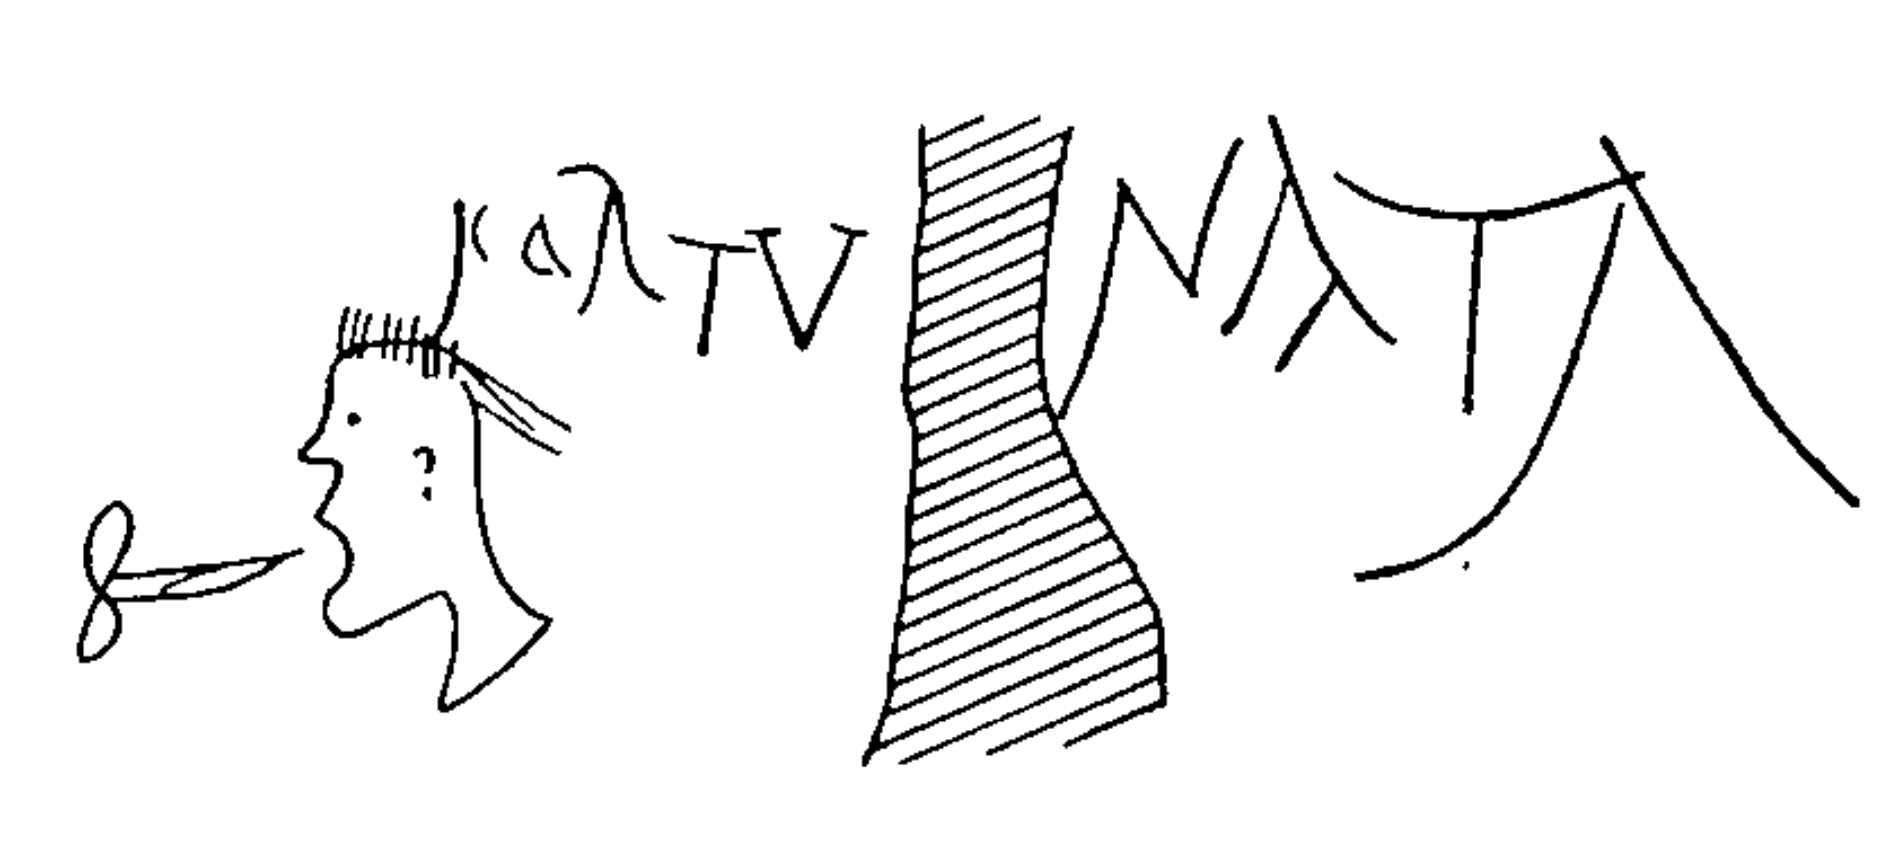
\includegraphics[width=\linewidth]{figures/chap1/part3/graffiti.png}
        \caption{Pompéi, I, 9, 5. Graffiti de \textit{Fortunata} faisant une fellation. CIL, IV, 10005.}
    \end{minipage}%
    \hfill
    \begin{minipage}{0.45\linewidth}%
        \centering
        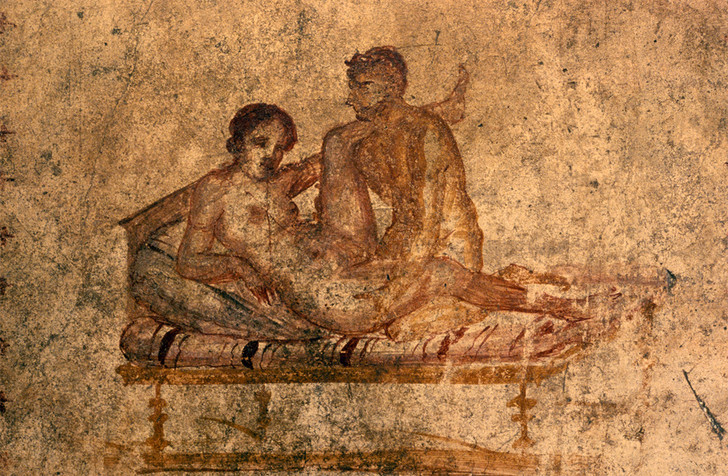
\includegraphics[width=\linewidth]{figures/chap1/part3/vettii.jpg}
        \caption{Peinture érotique d'une pièce attenante à la cuisine de la maison des Vettii (VI, 15, 1). I\textsuperscript{er} siècle. \textcopyright Getty.}
    \end{minipage}%
    \\
    \begin{minipage}{0.45\linewidth}%
        \centering
        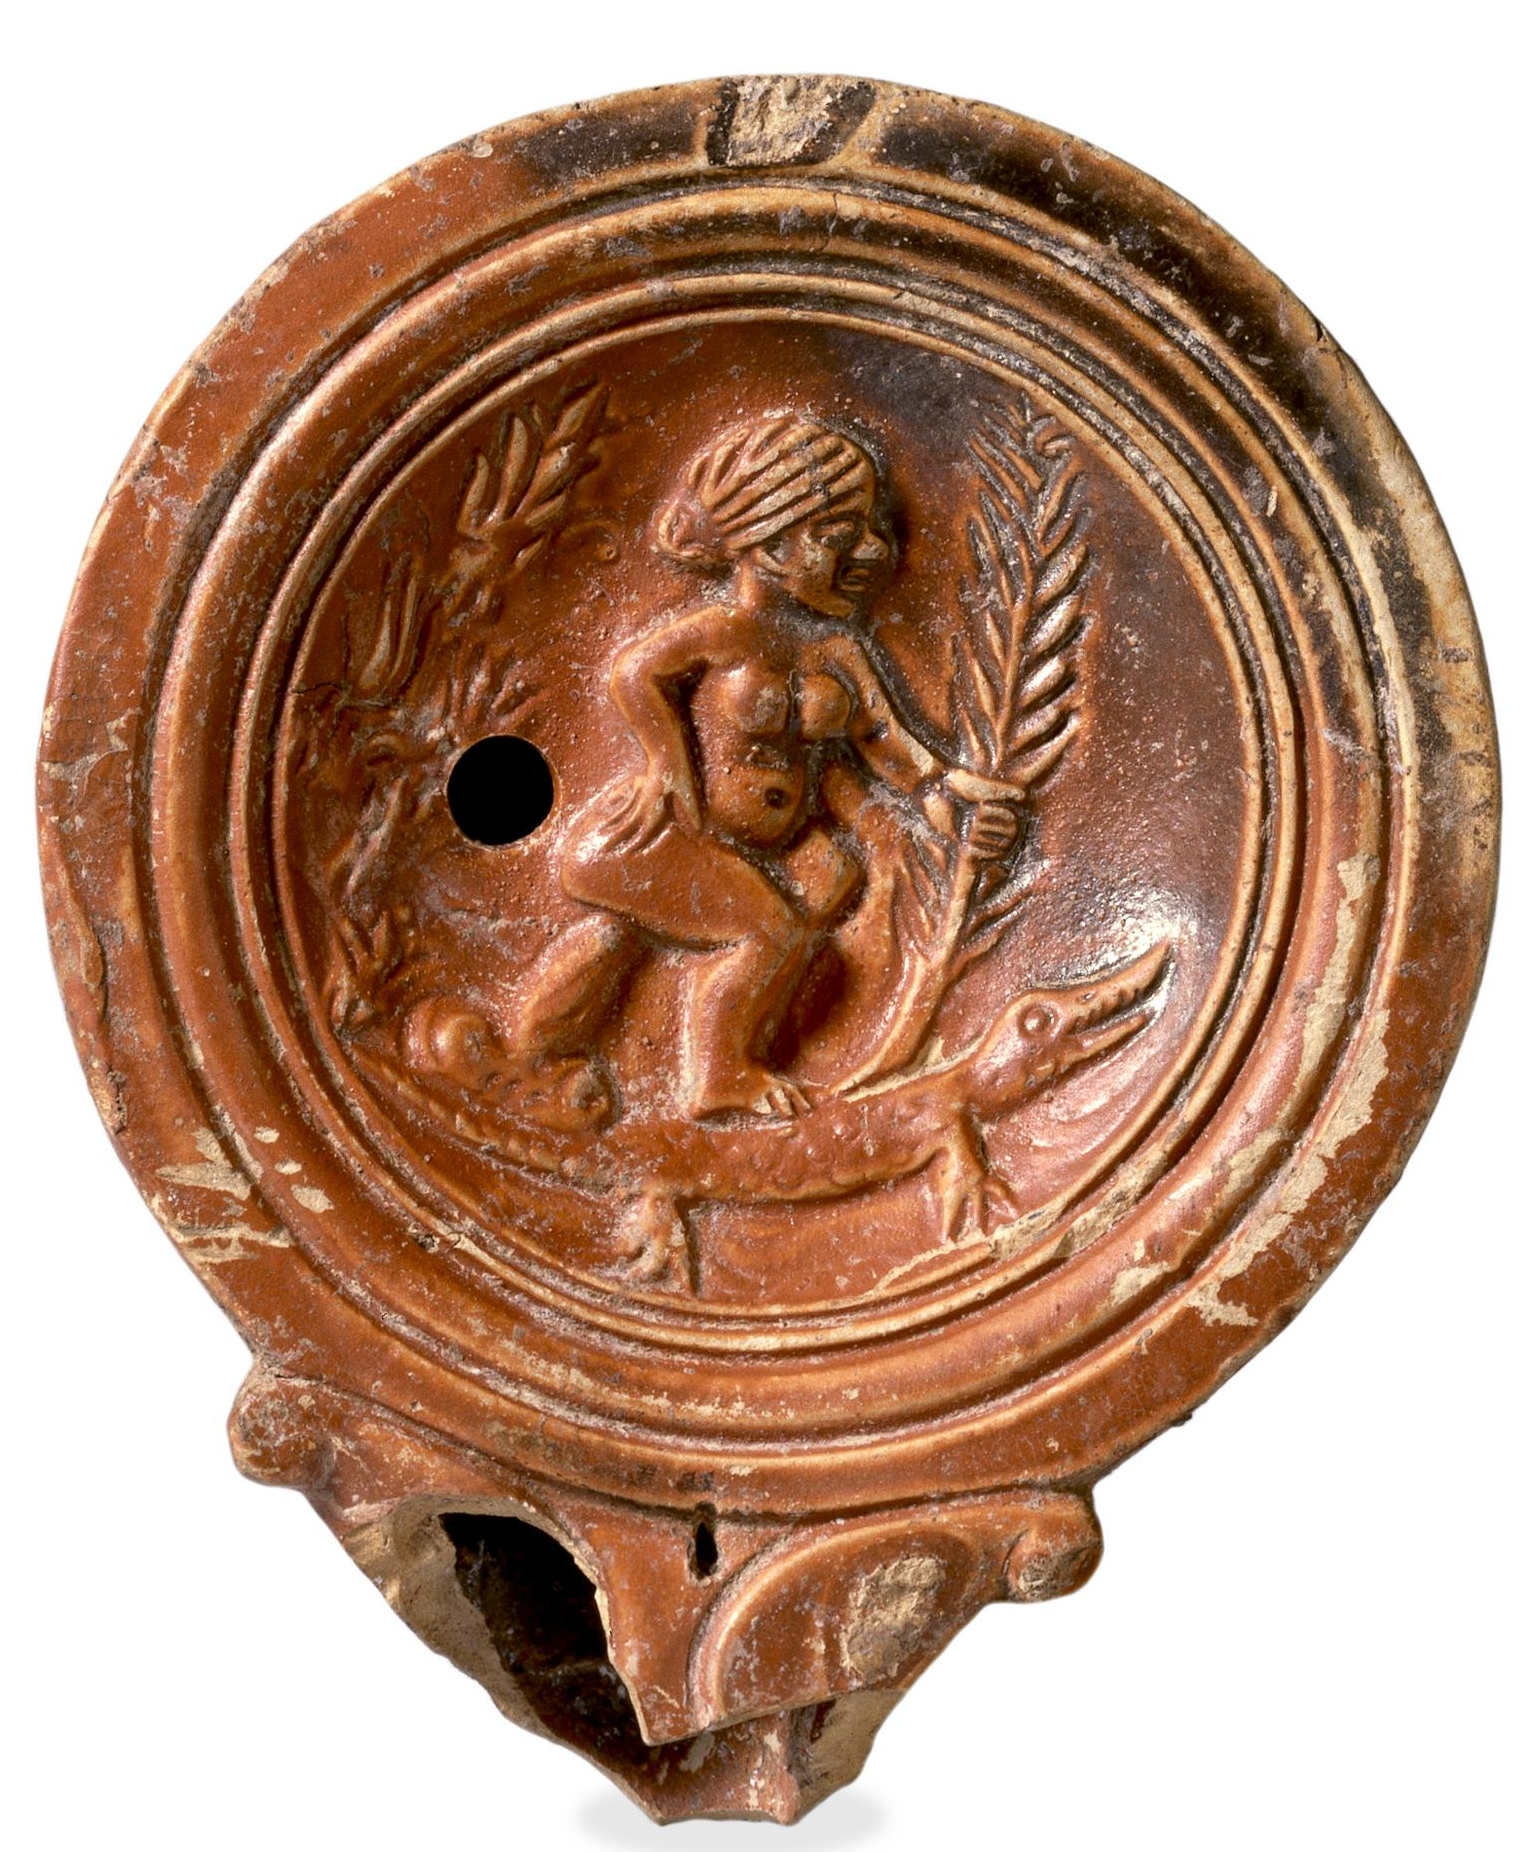
\includegraphics[width=\linewidth]{figures/chap1/part3/36916001.jpg}
        \caption{Lampe en terracota figurant une scène soit d'agalmatophilie avec un Priape, soit de masturbation avec un godemichet. Le personnage est une naine noire égyptienne, caractéristique d'une tendance artistique du I\textsuperscript{er} siècle de notre ère. Entre 50 et 75 d'après Paul G.~P.~Meyboom et M.~J.~Versluys\footcite{meyboom2006meaning}. \textcopyright British Museum, CC-BY-SA-NC.}
    \end{minipage}%
    \hfill
    \begin{minipage}{0.45\linewidth}%
        \centering
        \includegraphics[width=\linewidth]{figures/chap1/part3/Tintinnabulum_Pompeii_MAN_Napoli_Inv27854.jpg}
        \caption{\textit{Tintinnabulum} représentant un Mercure ityphallique. Il manque les clochettes. Museo Archeologico Nazionale di Napoli (inv. 27854).  \textcopyright Marie-Lan Nguyen / Wikimedia Commons / CC-BY 2.5}
    \end{minipage}%
    \caption{Exemples de l'omniprésence des représentations de la sexualité dans la vie romaine.}
    \label{fig:chap1:planche1}
\end{figure}
\clearpage
}

Concernant Rome, on commence à traiter de sujets plutôt personnels, de la vie privée, comme celui de la masturbation\footcite{krenkel_masturbation_1979}. Le travail de Paul Veyne sur l'\textit{Élégie érotique}\footcite{veyne_lelegie_1983} ou l'\textit{Homosexualité à Rome}\footcite{veyne_homosexualite_1982}, se servant à la fois de Michel Foucault et des travaux sur la Grèce de K.~J.~Dover\footcite{dover_greek_1979}, démarre côté français une étude de la sexualité et de l'érotisme romains. Le début des années 1980 reste d'abord un tâtonnement, une phase de questionnement majoritairement conduite à partir de catégories modernes et occidentales. Bien que l'anachronisme permette de poser des questions en histoire\footcite{loraux_eloge_2005}, l'usage de catégories d'analyse contemporaines, comme l'homosexualité, pose un certain nombre de problèmes: la sexualité de même sexe à Rome n'est pas perçue comme opposée à l'hétérosexualité. 

Les années 1990 voient une production de référence avec notamment les travaux d'Amy Richlin\footcite{richlin1992pornography, richlin1993not} ou d'Eva Cantarella\footnote{Publié en 1988 puis traduit en anglais en 1992, \textcite{cantarella_bisexuality_1992, cantarella_secondo_1988}}.%
% Reprendre la relecture ici, page 100
Dans l'ouvrage collectif qu'elle dirige, Amy Richlin entend inscrire son travail dans les \textit{cultural studies}, cherchant donc à donner voix à ce qu'elle perçoit comme les minorités romaines, tout en appliquant les \enquote{théories féministes ou d'autres théories modernes\footcite[p.~XI]{richlin1992pornography}}. Son objectif est aussi de permettre aux \textit{classicists} de reprendre la main sur l'historiographie de la sexualité, et d'aller à l'encontre de ceux \enquote{qui chercheraient la salvation de l'humanité dans un âge d'or passé\footcite[p.~XVIII]{richlin1992pornography}}. Il est alors question de mettre en place un cadre de lecture féministe des textes anciens: se pose la question de la représentation du viol ou en général des violences faites aux femmes. Molly Myerowitz parle ainsi du \enquote{sexisme} ou du \enquote{sadisme} envers les femmes chez Martial, Horace et Juvénal\footcite{myerowitz1992domestication}. Mais ces travaux sont critiqués\footcite{frontisi2004ovide}, pour leur angle et les présomptions effectuées sur la réception des textes par les femmes romaines: une approche émique de la lecture des textes littéraires latins en utilisant des concepts étiques se confronte nécessairement à l'absence de sources et à l'incompatibilité des systèmes, le discours rapporté par les documents transmis étant uniquement celui du groupe dominant\footnote{Tant bien que même si nous avons des textes de femmes, ils seraient probablement aussi issus de cette appréciation de la réalité. \textcite{cuchet_hommes_2011}}.

Les années 2000 puis 2010 voient la naissance -- en France au moins -- d'un renouveau historiographique, héritier en grande partie des pratiques du centre Gernet et des Annales. La question d'un renouvellement des points de vue, quitte à utiliser des approches étiques et donc des anachronismes pour les questionner, permet l'émergence d'une nouvelle histoire de la sexualité, en opposition partielle des approches américaines. Sur la question des sexualités romaines, Florence Dupont et Thierry Éloi préfèrent par exemple les termes homophilies et homoérotismes à celui d'homosexualité\footcite{dupont_antiquite_2013}: il s'agit de différencier alors l'homosexualité identitaire, subie au XIX\textsuperscript{e} puis revendiquée en deuxième partie du XX\textsuperscript{e}, de l'acte sexuel entre deux personnes du même sexe biologique. Il s'agit aussi d'explorer la question des différents objectifs des actes sexuels (récréatifs, reproductifs), de ses interdits, de sa perception et des discours qui les entourent. Géraldine Puccini\footcite{puccini_delbey_vie_2010} cimente ainsi un peu plus les fondements d'une sexualité liée aux statuts (esclave, affranchi, libre, femme mariée, citoyen, etc.) et perçue comme l'on perçoit n'importe quel excès le cas échéant. Le débat historiographique tourne majoritairement -- pour la sexualité masculine -- autour de la thèse de P.~Veyne d'une \enquote{bisexualité active qui suppose la valorisation d'une sexualité virile et conquérante}\footcite[p.~20]{puccini_delbey_vie_2010}, et chacun se situe donc en fonction de cette dernière. Enfin, la sexualité féminine est étudiée\footcite{girod_les_2013}, confirmant une dichotomie entre la femme mariée, au rôle reproductif, et la prostituée, au rôle récréatif, avec des variations entre les deux pôles. On traite enfin d'autres sujets que le simple plaisir masculin: le plaisir féminin et le discours qui s'y rapporte, notamment chez Ovide, prennent leur place dans cette historiographie renouvelée.

En parallèle, la sexualité romaine s'affiche à travers des ouvrages grand public en histoire de l'art. Les travaux illustrés de Catherine Johns\footcite{johns2000sex} ou d'Eva Cantarella\footcite{cantarella_pompei_2000} ont par exemple une vocation: montrer et faire comprendre l'omniprésence du sexe dans la vie et la ville romaine (\textit{cf.} planche \ref{fig:chap1:planche1}). Pour l'époque contemporaine, cette représentation constante des \textit{phallus} et des actes est troublante: du \textit{tintinabullum}, sorte de lampe à clochette permettant par exemple de rejeter le mauvais sort, mais aussi d'annoncer l'ouverture des bains, aux peintures érotiques et graffiti sur les murs, le sexe est partout. Une catégorie d'objets est probablement la plus représentative de cette diversité: les lampes à huile en terracotta, faisant figurer aussi facilement gladiateur que toute une variété de scènes de sexe. Ont été recensées sur ces supports les classiques scènes de fellation, pénétrations anales et vaginales. Les acteurs, leur nombre et les positions y varient fortement: femmes, hommes, nains, dieux, animaux\footnote{Sur ce sujet, la collection du \textit{Romisch-Germanisches Museum} est exemplaire.}. Ce renouvellement, encore bien timide dans de nombreux musées\footnote{Pour préserver la jeunesse d'une telle image ?}, permet de lier archéologie et analyse des textes pour renouveler notre compréhension de cet aspect de la Rome antique.

\paragraph{Le renouvellement lexicographique}

De ce changement d'attitude vers Rome nait un renouveau du travail lexicographique. Jusqu'aux débuts des années 1970, le travail se concentre plutôt sur le parler populaire\footcite{otto_sprichworter_1890} ou la vulgarité latine\footcite{opelt1970schimpfworter} ou encore le style figuré\footcite{opelt1966euphemismus}. Puis, cette décennie voit émerger un un travail directement centré sur la sexualité et son lexique: en 1973, à travers la thèse d'Enrico Montero Cartelle\footcite{montero_cartelle_aspectos_1973} qui nous est connue par M.~Dubuisson, puis en 1978 à travers celle d'Amy Richlin\footcite{richlin_sexual_1978} \textit{Sexual Terms and Themes in Roman Satire and Related Genres}. Les deux auteurs font d'ailleurs de ce domaine une spécialité: E.~Montero~Cartelle continue à publier sur la question sexuelle ou à éditer des textes sur le domaine, principalement du bas Moyen Âge (\textit{De Coitu} par exemple); Amy Richlin est particulièrement connue pour son travail sur l'histoire des femmes et de la sexualité, comme il a été vu plus haut. 

\begin{figure}
    \centering
    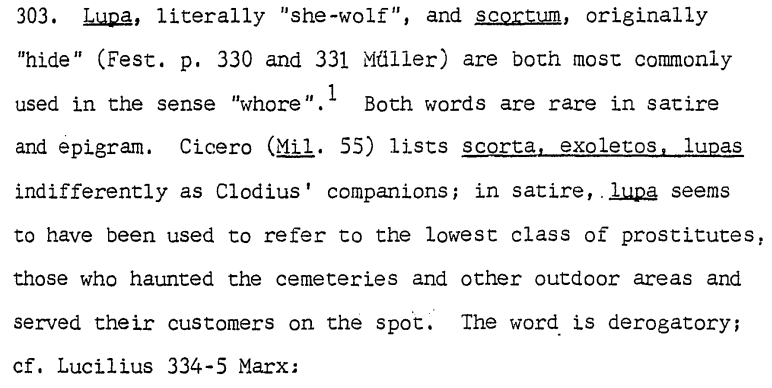
\includegraphics[width=.7\linewidth]{figures/chap1/part3/303_AmyRichlin.png}
    \caption{Exemple d'entrée (reproduite partiellement) de la thèse d'Amy Richlin}
    \label{fig:chap1:entry_richlin}
\end{figure}

Le travail d'Amy Richlin se passe de références aux travaux lexicographiques mentionnés plus tôt, mais établit, en trois chapitres, un état des lieux conséquent. Son premier chapitre et son second permettent d'établir un \enquote{cadre théorique} sur les questions des obscénités en latin et de réparti les sources sur la sexualités en deux sous-catégories, celle de l'érotisme et celle de l'invective. Contrairement à l'ouvrage qu'elle dirige en 1992, aucune mention n'y est faite des \textit{cultural studies} ou même de féminisme\footnote{Même le terme \textit{reception} n'y est jamais présent.}. Son chapitre trois est un \enquote{catalogue}, plutôt exhaustif dans ses références et dans son traitement de la langue, parfois extrêmement concis et plus proche du dictionnaire. Elle s'inscrit clairement dans la voie tracée par J.~Henderson, lexicographe helléniste, et son \textit{The Maculate Muse} publié en 1976 en lui reprenant ses subdivisions lexicales: \enquote{relation hétérosexuelles; physiologie; rôles hétérosexuels; homosexualité; sexe oral; prostitution; scatologie; caresse et masturbation; piéger et préparer des contextes favorables à la relation sexuelle; divers\footcite[\textit{Abstract}, p.~II]{richlin_sexual_1978}}. Ces catégories sont bien celles du XX\textsuperscript{e} siècle, anachroniques au possible, et se concentrent principalement sur le sexe des partenaires.

Amy Richlin laisse un flou quant aux limites de sa recherche, qu'elles soient génériques ou chronologiques. Du point de vue générique, elle mentionne dans le titre \enquote{la satire et les genres liés}. Ces genres sont en fait beaucoup plus larges que la satire: elle inclut volontiers les discours juridiques de Cicéron dans la catégorie \textit{invective}, mais utilise aussi les inscriptions non littéraires. Les genres plus attendus, comme l'élégie, sont bien sûr présents. Les bornes chronologiques sont courtes, mais floues: la période considérée semble se limiter principalement à l'antiquité classique ou du moins aux écrits païens. Cela exclut de fait des auteurs comme Ausone, dont le travail est inspiré fortement de Martial quand il s'agit de parler de sexualité, ou Apulée\footnote{Cité une fois en note de bas de page page 303.}, dont la peinture du désir masculin est assez exceptionnelle dans la littérature latine. Pour autant, l'\textit{Anthologie Latine} et les inscriptions font nécessairement bouger cette ligne temporelle vers l'antiquité tardive. Au final, la limitation générique est celle qui laisse le plus dubitatif: aucun des historiens latins n'est appelé en renfort par l'auteure pour appuyer les explications qu'elle produit, comme si les gens sélectionnés étaient auto-suffisant pour expliquer le lexique de la sexualité

Les entrées suivent la même structure: elles proposent un lemme et sa traduction ou un thème et les mots qui s'y rapportent (\textit{cf.} \enquote{circoncision}) suivis d'une explication sur les usages et des citations permettant de comprendre les usages du thème. Les entrées sont riches. Elle y décrit les connotations. Par exemple, pour \textit{cunnus}\footcite[p.~208]{richlin_sexual_1978}, l'auteure mentionne les usages poétiques, les exceptions à sa violence supposée, la phrase de Cicéron en \textit{Orat.} 154 pour montrer sa vulgarité\footnote{Cicéron indique dans ce passage qu’il faut éviter de dire \textit{cum nobis} (avec nous) car cela évoque le son de \textit{cunnus}. Il récidive dans sa lettre à Papirius Paetus (Fam. 9.22.2) en donnant la succession \textit{cum nos} comme fâcheuse à l'oreille. C'est ce que les grammairiens appellent un cacemphaton: voir \textcite{nicolas2007gros}.}, dressant ainsi un panorama complet. On retrouve les contextes d'usage, notamment les contextes génériques: pour \textit{lupa} par exemple, \textit{louve}, elle indique la rareté du terme pour parler de prostituées dans les satires et épigrammes, tandis qu'elle cite les usages de Cicéron\footcite[p.~329]{richlin_sexual_1978}.

En 1982, James Noel Adams publie son \textit{Latin Sexual Vocabulary}, qui constitue notre source principale pour notre exemplier et dont nous parlerons plus bas. Tout au plus peut-on noter une supposition ici sur la chronologie des travaux de J.~N.~Adams et d'A.~Richlin. Cette dernière ne publie jamais son travail de thèse, il n'est disponible que sous forme de microfilms du tapuscrit de 1978. Il est possible que les deux travaux se soient retrouvés en conflit sur le moment, et que celui d'A.~Richlin ait perdu la course à la publication commerciale, tout comme il est possible que la jeune docteure ait souhaité rediriger son travail sur une approche nouvelle du thème, moins lexicographique. Il reste la publication qui suit son travail de thèse, \textit{The Garden of Priapus: sexuality and aggression in Roman humor}, publié en 1983\footcite{amy1983garden}, réutilisant en partie ses travaux de recherche sans valoriser l'ensemble de ses recherches ni adopter la même approche du sujet.
% https://hal.archives-ouvertes.fr/hal-01800658v2/document

\begin{figure}
    \centering
    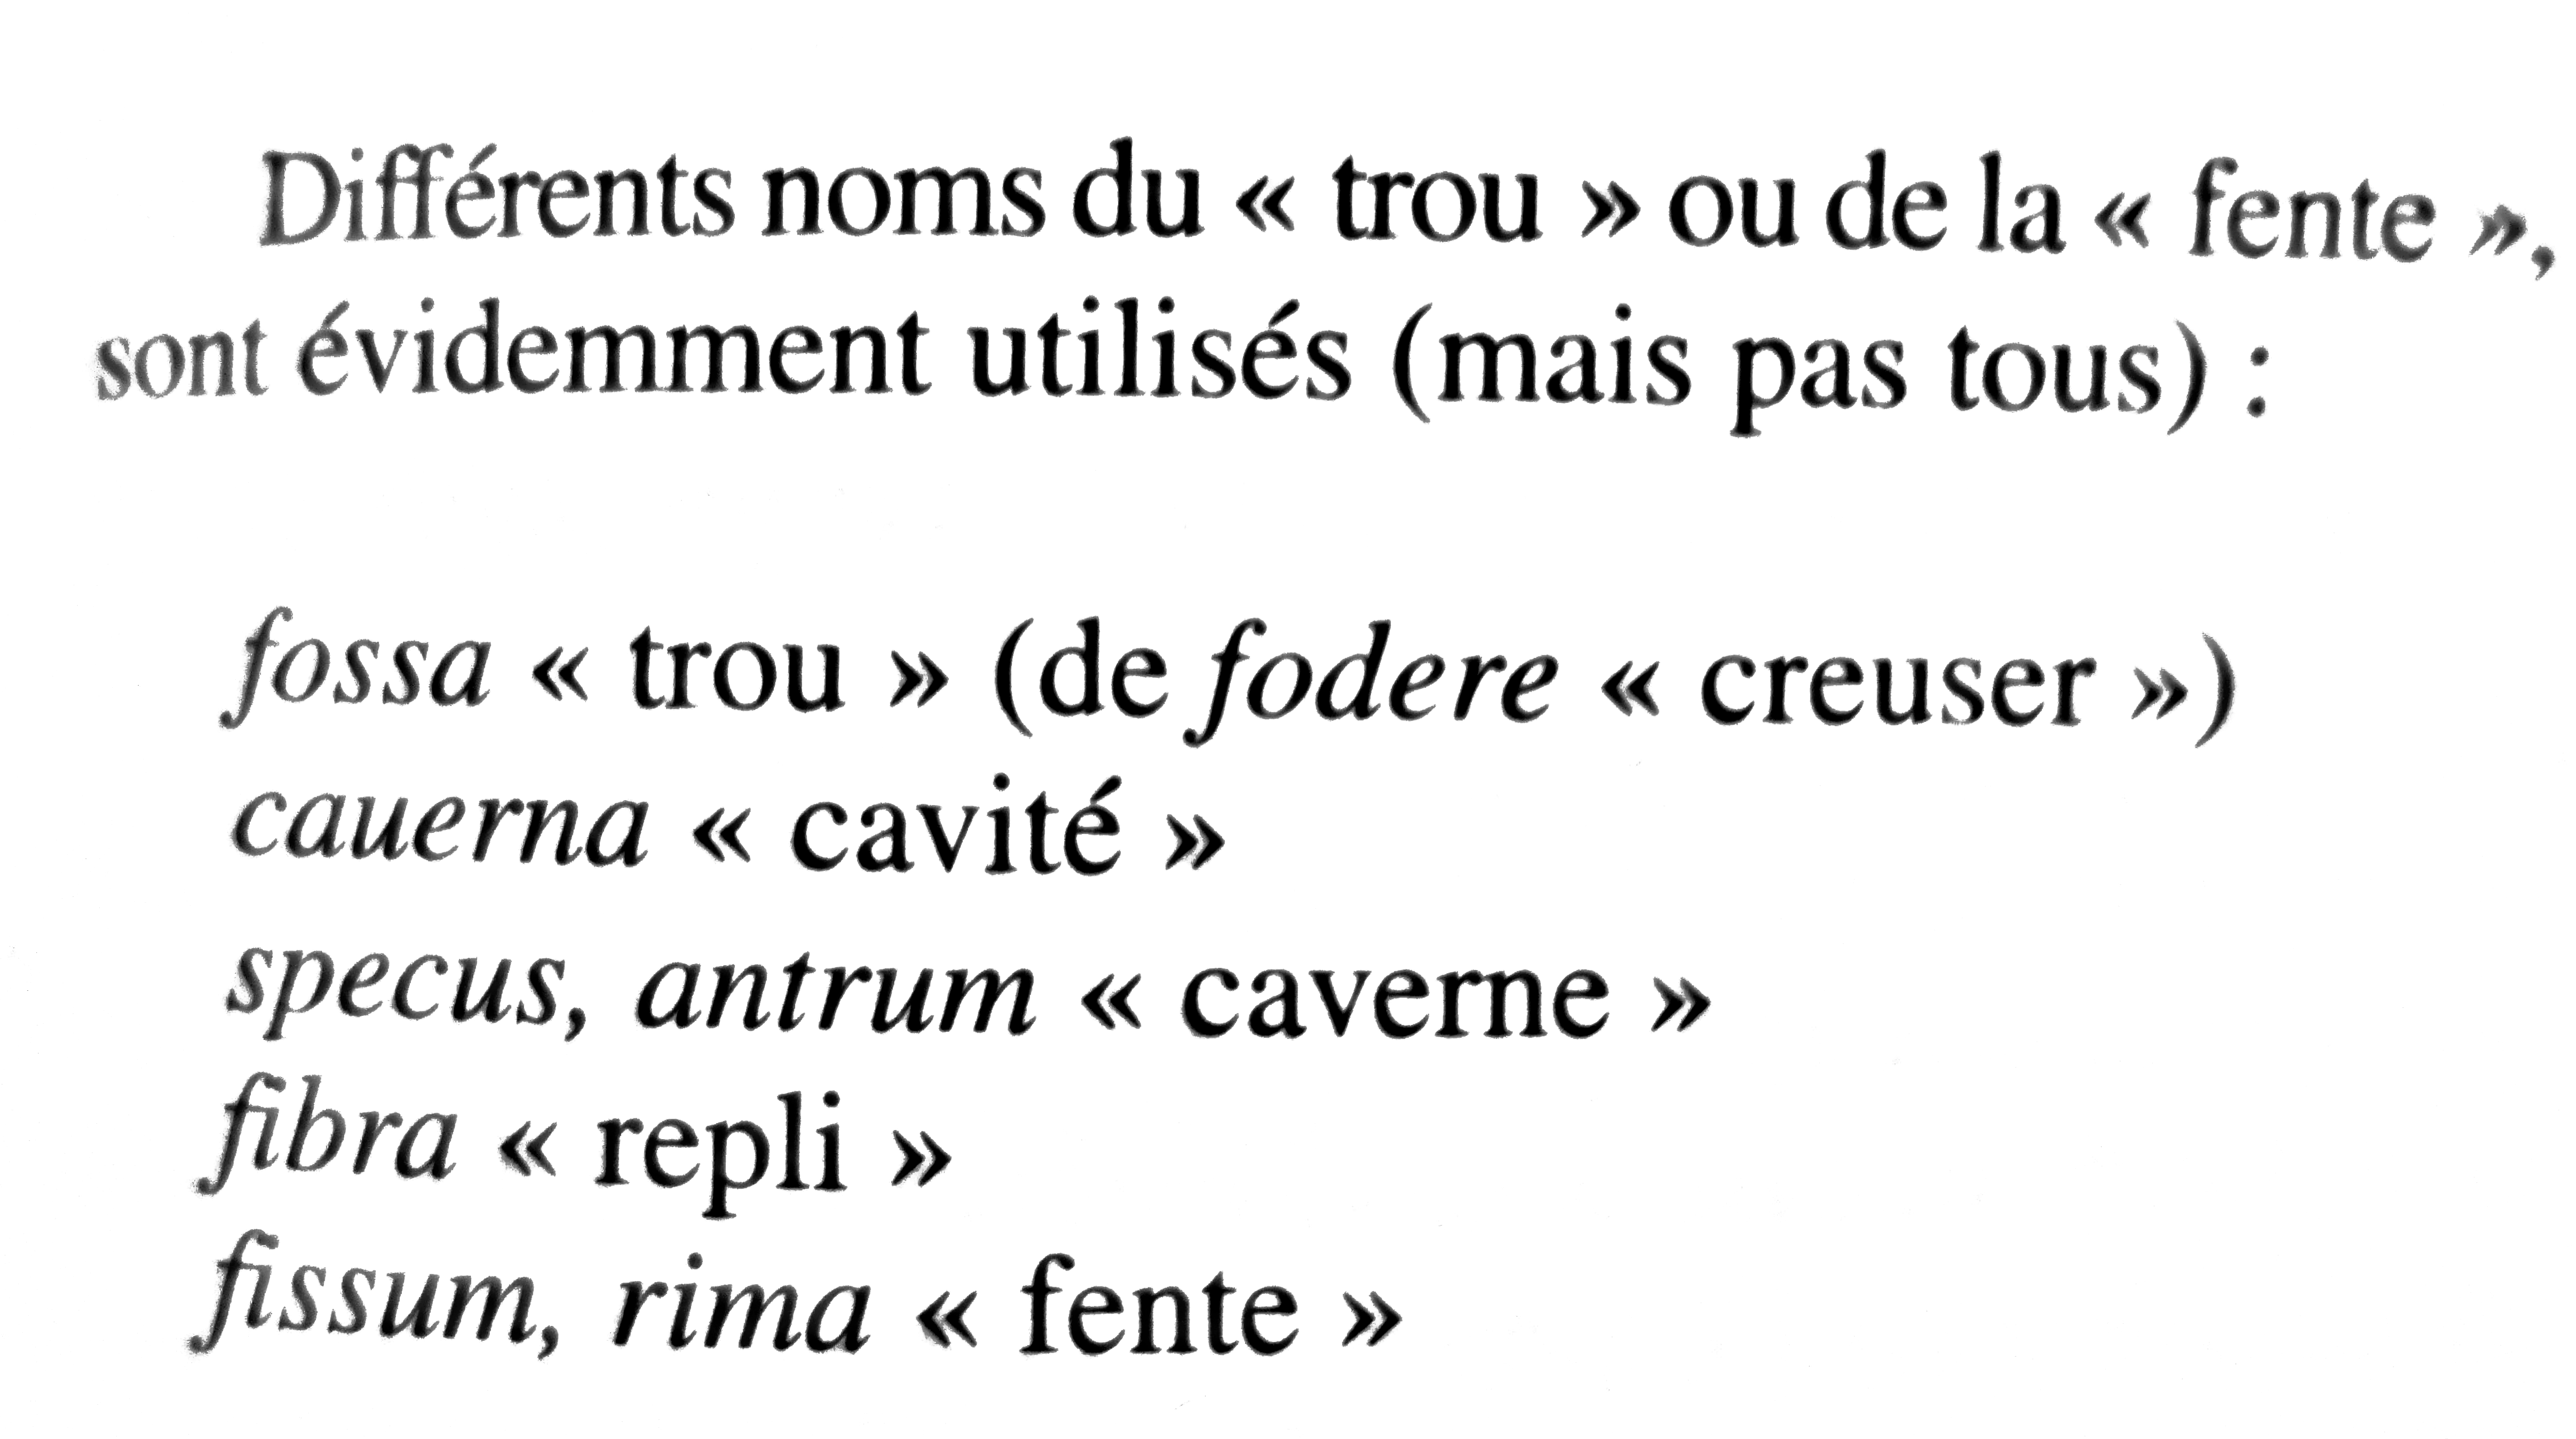
\includegraphics[width=.5\linewidth]{figures/chap1/part3/37_dubuisson.png}
    \caption{Exemple d'\enquote{entrée} de M.~Dubuisson, \textit{Lasciva Venus: petit guide de l’amour latin}}
    \label{fig:cap1:dubuisson}
\end{figure}

Il faut attendre Michel Dubuisson et son ouvrage publié à titre posthume en 2011 pour retrouver une approche lexicographique \enquote{complète} de la sexualité latine. Il y découpe le sujet en quatre parties: \textit{Femina} (corps féminin), \textit{Vir} (corps masculin), \textit{Antecenia} (Préliminaires), \textit{Effectus} (l'acte). Mais le travail de M.~Dubuisson se rapproche plus d'un travail de vulgarisation ou de satisfaction de curiosité intellectuelle que d'une publication scientifique traditionnelle, sans manquer d'érudition cependant. La maison d'édition (La Différence), le ton (\enquote{Ce charmant poème est tout simplement une plainte sur la débandade\footnote{Le qualificatif charmant et l'usage de \enquote{tout simplement} sortent un peu de la réserve universitaire classique. \textcite[p.~21]{dubuisson_lasciva_2011}}} et l'absence de bibliographie sérieuse (tout au plus quelques références) donnent l'impression que ce livre a d'abord vocation à être lu par des non-spécialistes. Il ne se veut pas exhaustif (\enquote{Je n'avais ni l'envie de faire un pavé rébarbatif, ni la compétence pour faire un \textit{Kamasutra} latin: j'ai dû choisir, c'est-à-dire éliminer\footcite[p.~13]{dubuisson_lasciva_2011}}) et ses choix sont \enquote{criticables} comme il le dit lui-même, peut-être même ancrés dans une vision de la sexualité romaine un peu datée. Mais l'on sent, au fil de la lecture, que c'est un sujet qui amuse, un livre léger, et qu'il s'agissait peut-être pour le linguiste belge de s'échapper un peu de sujets plus \enquote{graves} liés au latin. Il rejoint, nous semble-t-il, le travail de A.~Blondeau au XIX\textsuperscript{e} siècle: la sexualité est un sujet amusant, vendeur, il serait dommage pour l'auteur de ne pas se laisser tenter.


\subsubsection{J. N. Adams, la \textit{Manchester School} et son travail sur la sexualité}

C'est dans ce riche contexte que s'inscrit le travail de J.~N.~Adams, et en particulier sa monographie sur \textit{The Latin Sexual Vocabulary}\footcite{adams}. Mais, si cette effervescence autour des sexualités grecques et latines explose au même moment, il ne faut pas ignorer un contexte beaucoup plus local au travail de l'auteur du \textit{vocabulaire}: la \textit{Manchester School}. Pendant une dizaine d'années en effet, quelques chercheurs des départements de grec et latin à l'université de cette ville se sont spécialisés dans le traitement des obscénités de ces deux sphères linguistiques. Après avoir étudié ce contexte très particulier, nous entrerons dans le détail de l'œuvre de J.~N.~Adams.

\paragraph{La \textit{Manchester School} de lexicographie}

Le travail de James Noel Adams est absolument indissociable de l'université dans laquelle il a travaillé, à savoir l'université de Manchester. Au début des années 1980, trois de ses chercheurs au moins se concentrent sur la question des obscénités, tant en latin qu'en grec: Henry David Jocelyn (1933--2000), David Bain (1945--2004) et James Noel Adams (1943--2021). Deux de ces chercheurs, Jocelyn et Adams, sont des australiens émigrés, ayant partagé à quelques années d'écart les bancs de l'université de Sydney. Jocelyn a sa commencé sa formation universitaire dans les cours de R.~E.~Smith (1910--1978), professeur d'Histoire Ancienne, y compris à Manchester de 1953 à 1974\footnote{Adams parle d'une profonde influence du second sur le premier}. Il la poursuit au St John's College de Cambridge en 1955\footcite[p.~281--282]{adams_henry_2003}. Il fait son début de carrière à Sydney\footnote{Déroulé de carrière de Jocelyn à Manchester: 1960 \textit{lectureship}; 1964 \textit{senior lectorship}; 1966 \textit{readership}; 1970 \textit{personal chair}.} puis obtient la chaire Hulme de latin en 1973 à Manchester\footcite[p.~286]{adams_henry_2003}. Adams a un parcours similaire: étude pré-doctorales à Sydney puis études doctorales à Oxford avant de prendre un poste à Cambridge jusqu'en 1972 où il rejoint Manchester\footnote{Déroulé de carrière d'Adams à Manchester: 1972 \textit{lecturer}; 1982 \textit{reader}; 1993--1995 \textit{professor}; hiatus dans d'autres universités puis un retour comme membre honoraire à la fin de sa carrière, de 2013 à 2015. \textcite{adams_page_carreer}}. David Bain est au contraire un Britannique au \textit{cursus honorum}, St Andrews (Écosse) puis St John's College (doctorat), avant de devenir \textit{lecturer} pour le grec ancien en 1971 à Manchester\footcite{bain_obituary}. 

Ces trois chercheurs forment donc la \enquote{\textit{Manchester School}}, qui se distingue par le choix de travailler sur les obscénités dans les langues latines et grecques. L'appellation se retrouve à plusieurs endroits, la source de cette dénomination n'est pas claire, F.~R.~D. Goodyear, un ancien camarade de classe de Jocelyn au St John's College\footcite[p.~282]{adams_henry_2003}, semble la faire sienne dans son compte-rendu du livre d'Adams\footcite{goodyear_praefanda_1985}, bien qu'Adams cite un intérêt de la presse pour cette école dès 1983\footcite[p.~289]{adams_henry_2003}. L'auteur du lexique latin de la sexualité fait de Jocelyn le fondateur \textit{a posteriori} de cette école, à travers son article sur λαικάζειν\footcite{jocelyn_greek_1980} et les \enquote{huit autres publications sur la terminologie antique de la sexualité}\footcite[p.~290]{adams_henry_2003}. Il écrit d'ailleurs la préface du travail d'Adams dans sa traduction italienne de 1996\footcite{adams1996vocabolario} où il dresse une bibliographie du groupe. Le travail de Bain nous est connu principalement par cette dernière: il publie neuf articles sur le sujet entre 1978 et 1986, dont \textit{Apotropaic farting}\footcite{bain1986apotropaic}, et puis quelques publications \enquote{tardives} dont son article de 1991, \textit{Six Greek Verbs of Sexual Congress}, où il note justement qu'il s'agit d'une restitution d'un travail commenté dès 1982 dans le séminaire du département de latin organisé par Jocelyn\footcite{bain_six_1991}. 

Le travail de J.~N.~Adams tourne majoritairement autour de la question du latin vulgaire, et par extension seulement il finit par aborder sexualités et corps. Les premiers travaux d'Adams portent en effet en grande partie sur l'édition ou l'étude de phénomènes de langue populaire. Dans \textit{Latin Words for 'Woman' and 'Wife'}\footcite{adams1972latin}, il s'intéresse par exemple à l'usage de \textit{femina} pour désigner une nonne; même dans son travail sur l'ordre des mots en latin, c'est le parler potentiellement populaire chez Plaute (VO plutôt que OV) qui retient son attention\footcite[p.~95]{adams_typological_1976}. Il publie une édition de texte \enquote{vulgaire}, spécifiquement pour le statut de son écriture\footcite{adams_text_1976}: \enquote{[Ce texte] est remarquable par son langage hautement vulgaire. Il a reçu peu d'attention de la part des latinistes, bien qu'il fournisse des éléments importants pour les étudiants du latin vulgaire\footnote{\textit{[This text] is notable for its highly vulgar language. It has received little attention from Latinists, though it yields important evidence for the student of Vulgar Latin.} \textcite[p.~2]{adams_text_1976}}}. Ce travail donne lieu à plusieurs publications majeures sur le sujet du latin vulgaire, de 1979 avec \textit{The Vulgar Latin of the Letters of Claudius Terentianus (P. Mich. VIII, 467-72)}\footcite{adams_vulgar_1977} à \textit{An anthology of informal Latin}\footcite{adams2016anthology} à 2016, sa dernière publication massive.

Le début des années 1980 sont marquées par le travail spécifiquement lié à la sexualité pour J.~N.~Adams. Trois œuvres principales (1, 2, 3) sont à lister et plusieurs mineures (4):
\begin{enumerate}
    \item Un article sur le \textit{culus} et les mots qui y sont liés\footcite{adams_culus_1981};
    \item Une monographie, \textit{The Latin Sexual Vocabulary}, publiée en 1982;
    \item Un article sur les Prostitués et les mots pour les désigner en latin, annoncé dans l'œuvre précédente\footcite{adams_prostitute};
    \item Un article \textit{Martial, 2, 83} commentant le texte dont le titre est issu\footcite{adams_martial_1983}. L'auteur y refait un point sur le verbe \textit{irrumo} (\enquote{enfourcher une bouche}) qui termine le poème. D'autres textes, notamment son travail sur le \textit{Centon Nuptial} d'Ausone\footcite{adams1981ausonius}, complètent aussi son travail de lexicographie par des commentaires longs de quelques sources importantes pour le sujet.
\end{enumerate}
Dans au moins deux de ces travaux (\textit{Martial 2.83} et \textit{The Latin Sexual Vocabulary}), Jocelyn comme Bain sont remerciés\footnote{\enquote{\textit{D. M. Bain and H. D. Jocelyn made some useful comments on a draft of this paper}} dans \textit{Martial 2.83} en note de bas de page.}, le premier étant aussi remercié pour l'article sur le \textit{culus}\footcite[p.~264]{adams_culus_1981}. 

\paragraph{\textit{The Latin Sexual Vocabulary}}

La monographie d'Adams est publiée en 1982 chez Duckworth et fait l'objet de réimpression régulière. Elle est accompagnée dès sa sortie d'un \textit{Addenda and Corrigenda} ainsi que d'un chapitre annexe sur les fonctions biologiques hors reproductives (défécation, miction et les flatulences). L'ouvrage comporte 230 pages de rédaction hors préface, annexes, index, bibliographies. Une courte bibliographie principale avec ses abréviations est présentée dès après la préface, et elle est enrichie de références en note de bas de page.

% Le projet d'Adams
Adams présente un projet, en préface comme en introduction, ne cherchant pas à être exhaustif\footnote{\enquote{\textit{I should
not wish to claim that I have been absolutely exhaustive.}}\textcite[Preface, p.~1]{adams}} mais souhaitant \enquote{décrire et classer} la diversité que peuvent présenter les usages latins en matière de sexualités (et d'excrétions). Il s'agit d'un ouvrage rédigé, et non d'un glossaire. Il tourne autour de quatre domaines sémantiques précis, représentés par autant de chapitres, à savoir: le sexe masculin, le sexe féminin, les fesses, les actes sexuels. Ils suivent toujours une progression similaire (Mots de bases, Métaphores, Euphémismes, et, quelques fois, Divers) et s'accompagnent ensuite d'approfondissements spécifiques à chaque domaine, par exemple sur les différentes parties du sexe féminin ou le cas particulier de la masturbation du côté des actes sexuels.

% Couverture thématique: ce qui est présent ?

Chacune des grandes subdivisions de chapitre présente des regroupements: ils sont lexicaux quand il s'agit des termes de bases (\textit{Mentula} est divisé entre \textit{mentula} et \textit{verpa}), principalement stylistiques quand il s'agit d'euphémismes (\textit{pars pro toto}, parties adjacentes, etc.) et sémantiques pour les métaphores. La couverture d'Adams est donc assez large. Par exemple, pour \textit{Mentula}, la section métaphore propose entre autres les domaines sémantiques suivants: objets pointus, armes, objets ménagers, bâtons et choses similaires, objets agricoles, domaine botanique, domaine animale, etc. Adams se permet aussi de produire des sous-sections vides de termes, afin de traiter un domaine où une discussion lui semble nécessaire. Par exemple, pour le sexe masculin, il offre une réflexion sur l'usage de la métaphore du serpent en latin: pour lui, il n'y a rien qui corrobore un possible sème pénien à ces reptiles chez les anciens. Il ne s'agit pas alors de présenter les termes qui sont sexuels, mais ceux qui ne le seraient pas.


% Couverture thématique: Les manques
%   1. manque les adjectifs liés à la sexualité: Lascivus, mollis / mollitia, cinaedus qui n'est pas directement expliqué
%   2. manque les zones autres que sexuelles
%   3. Manque les questions de sex toy ? Aids and Manuals
%       3.a Check ancient sources Sexuality in Greek and Roman societyand literature : a sourcebook,
%   4. Manque des thèmes précis 


Le travail d'Adams démontre un certain nombres de manques. En termes d'avertissement, outre la préface qui annonce la couleur d'un travail massif mais \enquote{non exhaustif}, il annonce aussi page 118 que les termes les plus communs liés à l'acte sexuel seront moins documentés\footnote{\enquote{\textit{Various commonplace verbs and expressions are scarcely illustrated here, especially if the relevant article in the TLL is adequate.}} \textcite[p.~118]{adams}.}. La critique a remarqué cependant bon nombre de mots ignorés, non documentés et uniquement présents à travers des citations\footnote{Chez \textcite{rousselle_j_1987, richlin1984latin}}. Il est possible de répartir une partie de ces manques dans trois catégories: les adjectifs ou appellations spécifiques à la sexualité, les parties du corps sexualisées sans être des organes reproducteurs, et les \enquote{objets auxiliaires} à la sexualité.

Dans la première de ces trois catégories, les adjectifs ou appellations, on retrouve des termes permettent de mieux comprendre les nuances romaines et qui sont par ailleurs traités par A.~Richlin. Par exemple, \textit{lascivus} et les termes de sa famille arrive ainsi en huitième paragraphe\footcite[p.~147]{richlin_sexual_1978} dans son troisième chapitre, très tôt donc, et juste après \textit{futuo} et ses dérivés, \textit{criso}, \textit{salax} (traité rapidement par Adams\footcite[p.~206]{adams}). \textit{Lascivus} peut porter une signification non-sexuelle comme \enquote{joueur, badin} mais aussi pousser ce sens vers la \enquote{disponibilité sexuelle}, donnant ainsi le sens à son dérivé en français \enquote{lascif}. Cet écart d'Adams est d'autant plus intrigant qu'il ne s'empêche pas de traiter des mots proches du sens de \textit{lascivus}: ainsi, son \enquote{\textit{(v) Go, come to}\footcite[p.~175]{adams}} traite entre autres des termes signifiant \enquote{aller au bordel} ou \enquote{venir à quelqu'un en vue d'avoir une relation sexuelle}. D'autres termes suivent le même traitement: \textit{mollis} et sa famille\footnote{Mollis apparaît chez Adams dans des citations uniquement.} ou \textit{cinaedus} permettent par exemple de qualifier les partenaires sexuels. Le léxème \textit{moll-} sert notamment pour souligner la féminité\footcite{williams_meanings_2013} ou les \enquote{abus de plaisir\footcite[p.~320]{dupont_lerotisme_2001}} d'un homme, tandis que \textit{cinaedus} souligne le rôle sexuel du pénétré\footnote{\textcite[p.~142]{puccini_delbey_vie_2010}. \textcite[p.~275]{dupont_lerotisme_2001}.}.

La seconde catégorie et la troisième catégorie sont probablement beaucoup moins importantes en quantité que la première: les Romains ont tout une richesse de vocabulaire pour parler des partenaires ou des dispositions sexuelles, mais ils parlent moins, dans leur littérature, de certaines partie du corps ou d'objets dans ce contexte. Pour la catégories des autres parties du corps, F.~R.~D. Goodyear, dans son compte-rendu, remarque l'absence des baisers et de la poitrine\footcite{goodyear_praefanda_1985}. Les deux sont traités par Amy Richlin dans sa thèse. Sur le premier, une courte section\footcite[pp.~351--354]{richlin_sexual_1978} sur les baisers (\textit{basium, basio, basiolum, exosculor et osculum}) permet de découvrir un usage des baisers dans un contexte érotique (Pétrone) ou dans le cadre d'une relation à la fellation (en particulier chez Martial). Sur le second, l'auteure les mentionne et en offre une courte analyse\footcite[pp.~229--232]{richlin_sexual_1978}. Il semble que la poitrine, contrairement à la société contemporaine occidentale, ne soit que peu le lieu des fantasmes dans les sources latines. Chez les poètes considérés par la docteure, la mention de la poitrine (\textit{mamma}) se fait toujours dans une invective chez Martial. Au contraire, dans la comédie, elle est vue positivement (usage de diminutifs du type \textit{mammicula} dans Plaute, Pseud. 12961). Le reste des usages sont limités à une description des corps sans une érotisation particulière.

La dernière catégorie est la source d'un traitement plus limité du côté des lexicographes, entre autres car elle est assez rare. Adams, sans en faire une section ni un paragraphe à part entière, relève l'usage de \textit{scorteum fascinum} dans le sens de godemichet chez Pétrone\footcite[p.~63]{adams} mais ne s'étend pas sur le sujet. On retrouve plusieurs autres termes, qui, contextualisés, offrent ce sens dans les quelques travaux qui en parlent\footnote{Sur ce sujet, le plus grand nombre de références est chez \textcite{parker1997teratogenic}.}. Chez Ausone 78\footnote{Ausone, Épigramme 76 dans l'édition de B. Combeaud. \textcite[pp.~223-223]{butrica_myths_2005}.}, James. N.~Butrica propose un sens parallèle de \textit{lingere membra suae uxoris} (\enquote{lécher le membre de sa femme}) avec le \textit{lambere membra uirorum} (\enquote{lécher le membre des hommes}) du premier vers. Pour l'auteur, il s'agit ici d'un godemichet, et le jeu de l'épigramme tournerait autour d'un mari \textit{fellator} et d'une femme \textit{fututor}. Le même auteur refuse de voir un \enquote{clitoris géant} servant de phallus à Bassa en Martial, 1, 90\footnote{Adams propose la lecture de \textit{venus}$=$penis. \textcite[p.~98]{adams}. \textcite[p.~255]{butrica_myths_2005}.}: il propose de voir encore une fois un \textit{sex toy} dans \textit{prodigiosa Venus}. Sans qu'aucun mot ne désigne l'objet en particulier, il appuie sur le sens de \enquote{\textit{pedicare}} quand il s'agit de Philaenis qui \enquote{encule} de jeunes hommes en Martial, 7, 67\footnote{Sur Philaenis, en particulier chez Martial, lire \textcite{boehringer_not_2018}.}. Les godemichets par procuration ne sont pas non plus mentionnés: l'agalmatophilie et l'usage de Priapes en pierre est rejeté en note de bas de page dans le \textit{Latin Sexual Vocabulary}. Il n'y est d'ailleurs fait aucune mention des livres ou manuels liés à la sexualité\footcite[p.185]{puccini_delbey_vie_2010}: le livre d'Élephantis n'est pas mentionné malgré sa présence dans la \textit{Vie de Tibère} chez Suétone\footcite[p.~190]{gladhill_tiberius_2018}.

Au final, il nous semble que la couverture thématique d'Adams se concentre sur la sexualité mettant nécessairement en jeu \textit{mentula}, \textit{cunnus} ou \textit{culus}, et c'est cette sphère qui intéresse l'auteur, comme le montre son annexe sur excrétion et miction.

% Période couverte
%   1. En gros, origine du latin au Moyen Âge
%   2. Mais flou entretenu par l'auteur qui ne la définit pas, ce qui se ressent ici aussi.
%       2.a Très mauvaise couverture de la période chrétienne: dépendance du TLL et du canon littéraire ? Ou période chrétienno-tardive moins riche ?
%      2.b TLL et problème du TLL chez Adams

Parmi les autres critiques que l'on peut faire et que l'on a faites au travail d'Adams reste l'importante question des bornes chronologiques de son travail. Or, il n'en expose aucune. Dans le corps du texte, on retrouve quelques mentions du Moyen Âge notamment de Babio, auteur du XII\textsuperscript{e} siècle, cité douze fois, ou de \textit{William of Blois} (Guillaume de Champagne), auteur du même siècle que le précédent et cité autant de fois. Cette couverture, nécessairement imparfaite, semble par ailleurs se faire au détriment de l'antiquité tardive, dont la couverture semble être issue majoritairement des mentions trouvées dans le TLL, expliquant ainsi une concentration sur quelques auteurs très classiques (Augustin, Arnobe, etc.) au détriment de textes médicaux. La période classique est très bien représentée, en dehors des manques thématiques cités plus haut. Ce travail reste exceptionnel, et il faut le remettre dans le contexte de son époque: il n'y a, en 1982, ni CLCLT ni de PLD, la recherche est intégralement ou presque intégralement manuelle, et on ne peut être qu'impressionné par la masse de données récoltées par le mancunien.


% Pas de traduction ?
%  1. Adams dit que ça prend trop de place
%  2. Richlin dit que ça fait bizarre
%  3. Jocelyn dit que c'est normal pour un travail de lexicographe

On ne peut pas quitter la description du travail d'Adams sans le replacer à la fois dans sa relation au travail d'A.~Richlin, qui émet un compte-rendu du travail de son collègue australien, et dans son intégration au travail de la \textit{Manchester School}. Dans son papier sur Adams, Amy Richlin\footcite{richlin1984latin} déplore d'abord qu'Adams ne traduise pas, donnant lieu à des situations \enquote{bizarre}: elle cite à cet effet le refus de traduire en page 126 \enquote{Il ne \textit{fellat} pas}, que l'on pourrait rapprocher des pratiques du début du siècle où le latin obscène était laissé sans traduction ou en latin. Cependant, D.~Bain vient à la défense d'Adams\footcite[p.~408]{bain2014praefanda}, plusieurs années plus tard, sur ce même reproche qui lui est fait par une autre auteure\footcite{braund2002personal}:
\begin{quote}[\textit{Praefanda}]{D.~Bain}
    \enquote{[Elle souligne] l'effet libérateur de l'utilisation d'un langage désinhibé par cette dernière [Richlin]. Cela me semble obscurcir la distinction entre lexicographie et traduction. L'œuvre de Richlin abonde en traductions de passages, en particulier de vers latins, où les obscénités familières anglaises/américaines, si elles sont correctement appliquées (c'est un grand "si"), pourraient bien être utilisées comme une aide pour certains de ses lecteurs. De même, personne ne pourrait critiquer l'utilisation du langage vulgaire anglais dans les traductions proposées par Dover [...] puisqu'il tente de fournir à ses lecteurs des analogies, et que son sujet est plus sociolinguistique que lexicographique. L'étude plus austère d'Adams, en revanche, évite la traduction et vise à présenter un compte rendu lexicographique objectif du ton des mots ainsi que de leur sens. Compte tenu de son intention, il pourrait être considéré comme hasardeux d'avoir préjugé de la discussion en introduisant des termes vulgaires provenant d'une autre langue vernaculaire et d'une autre culture. Je suggère que les lexicographes, lorsqu'ils traitent de cette catégorie de vocabulaire, fassent preuve de prudence.}%
    \footnote{\textit{\enquote{[She stresses] the liberating effect of the use of uninhibited language employed by the latter [Richlin]. This seems to me to obscure the distinction between lexicography and translation. Richlin’s work abounds in translations of passages from, particularly, Latin verse where English/American colloquial obscenities, if correctly applied (this is a big ‘if’), may well be in place as an aid to some of her readers. Likewise, no one could criticize the use of English vulgar language in translations offered by Dover [...] since he is attempting to provide his readers with analogies, and his topic is more a sociolinguistic than a lexicographical one. Adams’s more austere study, on the other hand, eschews translation and is intended to present an objective lexicographical account of the tone of words as well as their meaning. Given his intention, it might be regarded as hazardous to have prejudiced the discussion by introducing low terms from another vernacular and another culture. I would suggest that lexicographers when dealing with this category of vocabulary should practise caution.}}}
\end{quote}
La raison derrière l'absence de traduction tiendrait alors d'une position de lexicographe prise par Adams, tandis que la traduction de Richlin, aussi \enquote{libératrice} soit elle, tiendrait principalement du fait qu'elle traduit les passages\footnote{Ce qui n'est pas tout à fait vrai, puisqu'elle traduit assez souvent les termes hors contexte, quand elle les introduit.}. Et à vrai dire, si l'on regarde les mots même d'Adams, il ne se défend pas ainsi: il cite, tout comme la question de l'exhaustivité, un problème de place s'il se mettait à tout traduire\footnote{\enquote{\textit{The book would be very much longer than it is if I had set out to translate the passages cited, or to discuss at length every crux containing a sexual usage.}}, \textcite[p.~VII]{adams}}. Adams traduit les termes assez souvent, et lorsqu'il ne le fait pas, c'est qu'il le catégorise (\enquote{\textit{Verpa can also be classified as a vox propria for the penis;\footcite[p.~12]{adams}}}).


% Adams, Manchester vs. The World
%   1. Adams et Richlin, un conflit d'approches ?
%   2. Adams et ses collègues: un tradition du bullying universitaire ?
%       Adams sur Jocelyn, page 291 => and then to endure a grilling, particularly from Jocelyn himself, at the end of the paper.
%       Jocelyn was usually sceptical about the attempts of some literary critics to find sexual puns in unlikely places, and this scepticism is nicely exemplified in ‘On some unnecessarily indecent interpretations of Catullus 2 and 3’, in American Journal of Philology , 101 (1980). Liverpool Classical Monthly , as its title suggests, gave contributors the chance to publish their thoughts without the reflection imposed by more conventional forms of publication. Jocelyn, typically, welcomed this opportunity for instant controversy. p. 290

Le deuxième grief qu'Amy Richlin oppose au travail d'Adams est son manque de \enquote{politesse\footnote{\enquote{\textit{A final word on courtesy}}, \textcite[p.~494]{richlin1984latin}}.}. Adams est particulièrement violent verbalement avec la littérature scientifique à laquelle il s'oppose, le relevé du comte-rendu est assez exemplaire: il qualifie ainsi le travail d'autres de \enquote{"\textit{totally implausible}" (p. 29, n. 2), "\textit{absurd}" (71, n. 3; 100, n. 1), "\textit{fanciful}" (155, n. 1), "\textit{far-fetched}" (171), "\textit{an absurdity}" (172), "\textit{quite unacceptable, . . ludicrous}" (210), "\textit{bizarre}" (211), or "\textit{so inaccurate that I have chosen not to refer to it}" (1, n. 2)\footcite[p.~494]{richlin_sexual_1978}}. Si l'on rajoute par dessus cela l'opposition des méthodes d'Amy Richlin et de James N.~Adams et le rejet du second du travail de Dover sur lequel la première fonde la structuration de son lexique, il est clair que le travail des deux est en conflit ouvert, comme le montre par ailleurs la reprise du sujet par Bain vue plus haut. Sur ce point, il est amusant de lire la personnalité qu'Adams peint quand il parle de son troisième collègue de la \textit{Manchester School}: Jocelyn aurait été connu pour sa capacité à \enquote{cuisiner} et à faire endurer aux participants de son séminaire ce genre de pratique\footcite[p.291]{adams_henry_2003}; il était de nature à chercher la \enquote{controverse à tout prix\footcite[p.290]{adams_henry_2003}}. Le vocabulaire d'Adams est probablement en partie issue de pratiques mancunienne ou d'une influence de Jocelyn sur sa propre manière d'écrire en 1984: après tout, Jocelyn a publié en 1980 un \enquote{\textit{On some unnecessarily indecent interpretations of Catullus 2 and 3}}.

Au final, le travail d'Adams, bien que non exhaustif dans les catégories qu'il couvre et incomplet en terme de thématiques abordées, est probablement devenue la référence sur le sujet du vocabulaire de la sexualité. Il couvre plus de huit cent termes dans quatre grands domaines, en contexte, et documente abondamment les éléments qui l'intéressent. Accompagné de ses articles sur le \textit{culus}, la prostitution, Martial et le \textit{Centon nuptial}, et en général de sa production de 1980 à 1985, il permet d'avoir accès à un panorama conséquent de la richesse lexicale et stylistique du latin pour parler de sexe.

% Compléter Adams ?
%   1. Le travail d'Adams pour compléter Adams
%   2. Les autres travaux

% 

\subsection{Un \enquote{exemplier numérique}}

Pour notre version de l'exemplier, nous utilisons uniquement \textit{The Latin Sexual Vocabulary} d'\textit{Adams} et ses sources secondaires, auxquelles il renvoie quand il ne souhaite pas donner -- par manque de place -- l'ensemble des références. L'exemplier numérique produit a donc deux buts: d'une part, il doit permettre une lecture humaine, d'autre part, il doit être facilement exploitable par la machine. Pour avoir une vue d'ensemble sur cet exemplier, nous discuterons d'abord les principes et la méthode de sa compilation. Nous développerons ensuite une analyse quantitative de l'exemplier numérique ainsi produit et traiterons brièvement de sa valorisation en dehors de l'apprentissage machine.

\subsubsection{Principes généraux}

% Bornes typologiques et chronologiques du corpus
    % Les données épigraphiques: pourquoi non.
        %% Difficulté de lemmatisation
        %% Présence relativement faible
    % Pas les données médiévales
    % Exception: les auteurs fragmentaires

% Format d'un exemplier numérique
    % Pas le premier mais combien publiés en TEI ou SQL ?
    %    Exemple : https://www.pantheonsorbonne.fr/page-perso/e0g411r066s
    %    Helene Castelli, http://theses.fr/2020PA01H075
    %    Eurykleia
    % Sourçable
    % Corrigeable (déjà des idées avec les bibliographies contradictoires ou supplémentaires)
    % Augmentable
    % Pas le premier mais vocation à être à la fois un corpus de recherche ET un corpus d'entraînement. Quel impact ?

Les exempliers numériques ne sont pas nouveaux, particulièrement en histoire ancienne ou en littérature, où la compilation d'extraits pour appuyer une recherche est assez commune et leur \enquote{perte}, notamment dans le cadre de travaux de thèse, encore plus fréquente\footnote{Par exemple, \textcite{castelli__2020, montreuil_histoire_2016}.}. Ces compilations dépassent rarement le stade d'annexes servant à la compréhension de la recherche et sont assez peu publiées en tant que résultats de la recherche. Or, ils pourraient permettre d'offrir une porte d'accès à des chercheurs débutants sur les questions qu'ils documentent, tout comme ils simplifieraient leur étude pour les spécialistes en épargnant à ces derniers de fastidieux relevés d'occurrences. Adams, quand il publie son œuvre, ne la pense pas comme un glossaire, contrairement à ses prédécesseurs. On peut probablement voir dans \textit{The Latin Sexual Vocabulary} une forme de base de données, mais c'est avant tout un commentaire scientifique. Passer d'Adams à un exemplier n'est donc pas seulement une collecte, c'est le fruit d'une interprétation du \enquote{récit} du philologue. Le passage au numérique de l'exemplier doit enfin savoir combiner cette collecte et cette interprétation en vue de les rendre opérables et pérennes.

Pour traiter toutes les facettes de cette création d'un exemplier numérique, nous commencerons par évoquer les différentes questions qui se sont posées à nous concernant le dépouillement du texte et les règles que nous nous sommes efforcées de suivre. Nous pourrons ensuite développer un cadre technique d'encodage des différentes informations nécessaires à la production de l'exemplier. Enfin, nous traiterons la problématique de l'outillage ayant permis notre compilation afin d'en éclairer les différentes subtilités.

\paragraph{D'Adams à un exemplier}

La première de ces questions est sans aucun doute celle des filtres appliqués à la collecte pendant la lecture du corpus. Nous distinguons trois catégories parmi ceux que nous avons mis en place, pour des raisons différentes. Le premier filtre exécuté est celui des typologies de documents: tout comme le meta-corpus dont sont tirés les exemples, nous avons exclu les données épigraphiques telles que les inscriptions, papyris, graffitis... Les motifs de cette exclusion sont d'ordre pratique. Les spécificités de ces documents épigraphiques -- par exemple l'absence de normalisation de l'orthographe -- ne permettent pas de les annoter linguistiquement de manière automatique: le traitement automatisé des langues ne s'est pas encore penché suffisamment sur cette forme de l'écrit en latin pour produire les corpus nécessaires à la production d'outils adaptés. Le second filtre appliqué est un filtre chronologique : nous n’avons pas inclus les œuvres qualifiées de \enquote{médiévales} par Adams. Ce dernier couvrant un large empan chronologique, allant de -250 à 1300, trois options s'offraient à nous. Nous pouvions élargir encore plus, en nous intéressant aux textes produits après 1300, mais la complexité d'accès à des versions numériques de la documentation tardo-médiévale nous a retenu de poursuivre dans cette voie. Nous aurions pu conserver la même tranche chronologique, mais en dépit d'efforts certains pour mettre à disposition des corpus de qualité (\textit{cf.} le projet Velum\footcite{bon2019challenges}), le problème de la disponibilité des textes (haut-)médiévaux restait là encore trop important. C'est donc la troisième et dernière option, celle de restreindre notre champ d'étude au latin classique et tardif, qui a été choisie: en plus de simplifier le problème des sources, un tel choix limite les complexités inhérentes à un travail sur la \enquote{longue durée}, particulièrement prégnantes pour les questions lexicographiques\footnote{Sur ce sujet, voir, entre autres, \textcite{gabay_lacteur_2015}.}. Il faut comprendre la raison pour laquelle Adams a cité ces extraits tardifs: il ne s'agissait pas de \enquote{documenter} le lexique latin de la sexualité, mais plutôt d'en souligner l'héritage, en particulier les phénomènes de spécialisation, dans les langues de l'an mil. Dans ce contexte, les extraits du médio-latin ont alors le même statut que les extraits des langues vernaculaires. Le dernier filtre pratiqué est celui des auteurs représentés dans le meta-corpus: si un texte n'est pas disponible dans ce dernier, ses exemples ne sont pas inclus dans l'exemplier, à l'exception des auteurs fragmentaires,  de toutes les manières assez peu cités. En contre-partie de ce choix, une liste des œuvres présentes chez Adams, mais absente du meta-corpus a été compilée.

La seconde des questions concernant le transfert de connaissances d'une monographie vers une forme de \enquote{base de données} est celle des données à inclure sur chacun des exemples. Il s'agit non seulement de prévoir leur exploitation dans un cadre computationnel, mais aussi d'interroger les futures lectures que le format permet. Ainsi, un exemple n'est pas qu'un corps de texte: c'est un extrait, et à ce titre il est produit par un auteur, issu d'une œuvre, elle-même publiée et éditée par un premier éditeur scientifique puis numérisée par l'un des projets cités \textit{supra}, comme \textit{Perseus}. Ces informations sont primordiales pour exploiter ce corpus par une lecture \enquote{humaine}, car elle permet de contextualiser et de retourner à la source en cas de nécessité. 

Un exemplier n'est pas un ouvrage à lecture linéaire. Il faut pouvoir y naviguer, soit par jeu de renvois depuis un document ou des mentions pendant une présentation orale pour un exemplier papier, soit par des liens ou des recherches à partir du moment où celui-ci est numérique. Dans ce but, nous devons ajouter aux extraits plusieurs informations supplémentaires. Nous ne pouvons pas toucher au livre d'Adams, mais, pour chaque exemple, on peut archiver la page à laquelle Adams le référence ou le cite. Plusieurs fois, surtout à partir du chapitre sur les actes, le philologue cite le TLL pour éviter de proposer une recension trop abondante pour un format papier: dans ce cas, on se doit de fournir à la fois la référence paginée de \textit{The Latin Sexual Vocabulary}, mais aussi celle du TLL qui est la source du dépouillement.

Adams propose aussi des catégorisations, ne serait-ce que par le titre de ses chapitres et sections. Ces classifications peuvent permettre une navigation supplémentaire \enquote{croisée}: là où le \textit{Vocabulary} propose de se déplacer de lieu en \enquote{lieu} dans une progression linéaire (\textit{Mentula}, \textit{Cunnus}, \textit{Culus}, Actes), l'exemplier numérique peut aussi permettre d'entrer dans le corpus via d'autres filtres. Par exemple, on peut approcher cet ensemble de données par le biais d'un domaine sémantique (la guerre, les armes) ou par un phénomène linguistique sélectionné par l'auteur (euphémisme, métaphore, etc.). On peut ajouter en plus de ces catégories disponibles à travers le \enquote{sectionnage} du travail lexicographique, des informations supplémentaires disponibles à travers le commentaire: par exemple, on peut distinguer dans les actes les extraits qui correspondent à ceux faits par les femmes sur les hommes.

Une recherche lexicale, option dont la simplicité d'usage dans un cadre numérique a dépassé celui de l'\textit{index verborum}, peut éventuellement s'ajouter aux précédentes approches de ces textes. La fonction principale attendue est probablement celle de la recherche de tous les passages présentant tel terme analysé par Adams, par exemple \textit{futuo} ou \textit{pedico}. Mais il est intéressant de dépasser cette limite et d'autoriser la recherche des mots présents dans le contexte d'une isotopie sexuelle. Par exemple, l'\textit{index verborum}, se concentrant sur les termes principaux du \textit{Vocabulaire}, ne permet pas de savoir dans quel contexte le lemme \textit{tu} apparaît et s'il est surreprésenté par rapport au meta-corpus. Une rapide recherche sur la forme \textit{tu} donne cinquante-neuf résultats, soit 0,13\% des mots de l'exemplier, tandis que la même recherche sur le meta-corpus donne 0,09\%, soit une augmentation de presque moitié de sa fréquence relative dans les extraits traitant de sexualité. De même, \textit{hic} (suivant le contexte ici ou démonstratif masculin singulier nominatif) a une fréquence relative de 0,15\% contre 0,09\% dans la littérature latine disponible ici. Ces deux spécificités statistiques peuvent donner des informations: par exemple, le redoublement du pronom, au vocatif ou au nominatif, et la capacité à désigner un lieu ou un objet caractérisent probablement une forme d'invective. En dehors de recherche statistique, on peut aussi s'intéresser aux contextes spécifiques de certains mots \enquote{intrinsèquement non sexuels}, par exemple \textit{anima} (l'âme), afin de mieux cerner les dimensions d'une occurrence particulière dans un commentaire.

\paragraph{Encodage}

% D'abord le schéma TEI
À partir de ces besoins théoriques, il faut produire un cadre technique favorisant la résolution de l'ensemble des problèmes exposés. Comme pour le meta-corpus, les questions de pérennisation et d'insertion dans un écosystème scientifique numérique restent primordiales: à ce titre, la TEI est la seule option à même de fournir une réponse à ces problématiques, à travers son statut de standard dans la communauté des humanités numériques pour la mise à disposition de textes enrichis.

Un principe de réalité s'impose cependant: l'exemplier, tout comme il n'a pas vocation à être lu linéairement, n'a pas vocation à être rédigé linéairement; il est une collection de micro-documents rassemblés dans un document maître. Pour produire ce système, deux options techniques s'offrent à nous. La première est celle des \texttt{<teiCorpus>}, qui représenteraient alors l'ensemble des extraits comme des documents indépendants réunis sous la forme d'un corpus maître avec ses propres métadonnées. La seconde est celles de \texttt{<div>}, qui représenteraient alors un seul document fait de nombreux et divers éléments. Produire pour chaque extrait un document TEI complet aurait été extrêmement verbeux, vu leur nombre (plus de deux mille cinq cents) et leur longueur (le passage le plus long  est de quatre-vingt-douze mots). Nous adoptons donc une approche où chaque extrait est une \texttt{<div>} en spécifiant son statut: c'est un fragment, extrait d'une œuvre plus large qu'il nous faut identifier.

\begin{figure}
\begin{lstlisting}[language=XML]
<div type="fragment" ana="#acte #disgrace #metonymie">
    <bibl corresp="#adams">
        <author>J. N. Adams</author>, <title xml:lang="lat">The Latin Sexual
            Vocabulary</title>, <biblScope unit="page">200</biblScope>
    </bibl>
    <bibl type="source">
        <author>
            <persName xml:lang="fr">Sénèque le Père</persName> [<persName xml:lang="eng"
                >Seneca, Lucius Annaeus, ca. 55 B.C.-ca. 39 A.D. (Seneca the
                Elder)</persName>] <idno type="VIAF"
                >https://viaf.org/viaf/23497389/</idno><idno type="LC">n82-166595</idno>
        </author>, <title xml:lang="lat">Excerpta Controversiae</title>, <biblScope
            unit="ref">6.8</biblScope>
        <idno type="CTS_URN">urn:cts:latinLit:phi1014.phi002.perseus-lat1</idno>
    </bibl>
    <quote xml:lang="lat" source="urn:cts:latinLit:phi1014.phi002.perseus-lat1:6.8"
        type="chapter">
        <w n="6.8" lemma="incestus2" pos="ADJqua"
            msd="Case=Nom|Numb=Sing|Gend=Fem|Deg=Pos">Incesta</w>
        <w n="6.8" lemma="sum1" pos="VER"
            msd="Numb=Sing|Mood=Ind|Tense=Pres|Voice=Act|Person=3">est</w>
        <w n="6.8" lemma="etiam" pos="ADV" msd="Deg=Pos">etiam</w>
        <w n="6.8" lemma="sine" pos="PRE" msd="MORPH=empty">sine</w>
        <w ana="#acte #disgrace #metonymie" n="6.8" lemma="stuprum" pos="NOMcom"
            msd="Case=Abl|Numb=Sing">stupro</w>
        <w n="6.8" lemma="qui1" pos="PROrel" msd="Case=Nom|Numb=Sing|Gend=Fem"
            >quae</w>
        <w n="6.8" lemma="cupio" pos="VER"
            msd="Numb=Sing|Mood=Ind|Tense=Pres|Voice=Act|Person=3">cupit</w>
        <w n="6.8" lemma="stuprum" pos="NOMcom" msd="Case=Acc|Numb=Sing">stuprum</w>
        <w n="6.8" lemma="." pos="PUNC" msd="MORPH=empty">.</w>
    </quote>
</div>
\end{lstlisting}
    \caption{Exemple numéro 2172, issu des Priapées}
    \label{fig:chap1:part3:exemple_xml}
\end{figure}

Afin de fournir le plus d'informations possible sur la provenance du document, on distingue trois types d'informations bibliographiques, dont la dernière est optionnelle:
\begin{enumerate}
    \item La bibliographie de type \enquote{source primaire}, qui permet d'identifier l'auteur ou l'œuvre antique, la référence canonique qui y est liée et l'identifiant du texte dans le meta-corpus. Elle est appuyée d'identifiants de la \acrfull{VIAF} et de la \acrfull{LC} afin d'intégrer le document dans un réseau de métadonnées bibliographiques.
    \item La bibliographie de type \enquote{source secondaire}, qui est presque uniquement constituée du \textit{Latin Sexual Vocabulary} et le TLL pour l'instant. Elle permet de revenir au commentaire original, via une pagination obligatoire, pour corriger ou mieux comprendre une interprétation philologique.
    \item La bibliographie additionnelle, qui n'est pas encore utilisée dans l'exemplier, mais dont l'inclusion future est prévue du point de vue de la structure TEI. Elle permet de faire état d'arguments contradictoires de la part d'autres spécialistes, qu'ils viennent de comptes-rendus ou de documents plus récents, pour faire apparaître le débat scientifique. Bien qu'elle soit aussi constituée de sources secondaires, à la différence du type (2), elle n'a pas servi à intégrer le passage dans la base de données, mais complète sa lecture. La pagination y est obligatoire.
\end{enumerate}

Enfin, le document contient un passage, pris sous la forme de citation (\texttt{<quote>}) qui reprend l'identifiant CTS intégral du passage. Les mots et signes qui le composent sont traités indifféremment par des \texttt{<w>} qui portent des informations linguistiques et syntaxiques: lemme, POS et informations morphosyntaxiques comme le cas\footnote{Nous développerons ces différentes informations plus tard dans le présent document, en chapitre 3.}. Exceptionnellement, on peut retrouver en plus des notes qui accompagnent l'extrait, et des traductions pourraient être ajoutées en supplément de la citation.

\paragraph{Outil(s) pour la compilation}
% Ensuite l'outil avec les "deux périodes de l'outil"

Un outillage n'est pas neutre, et en ce sens, documenter le plus possible les différentes méthodes de compilation permet d'expliquer, au besoin, des biais de corpus. La compilation du corpus s'est faite avec une interface conçue par nos soins. Cette interface, qui a connu deux versions, a toujours servi le même objectif: à partir de quelques champs, permettre de consigner un puis plusieurs extraits avec les informations nécessaires pour respecter le schéma expliqué précédemment. Pour ce qui est du résultat final, en dehors de quelques modifications de schémas et d'harmonisation suite aux divers changements techniques, seuls les identifiants VIAF et LC sont des introductions \textit{a posteriori}: à partir des diverses informations auteurs, on a pu ajouter des identifiants externes.

\begin{figure}
    \centering
    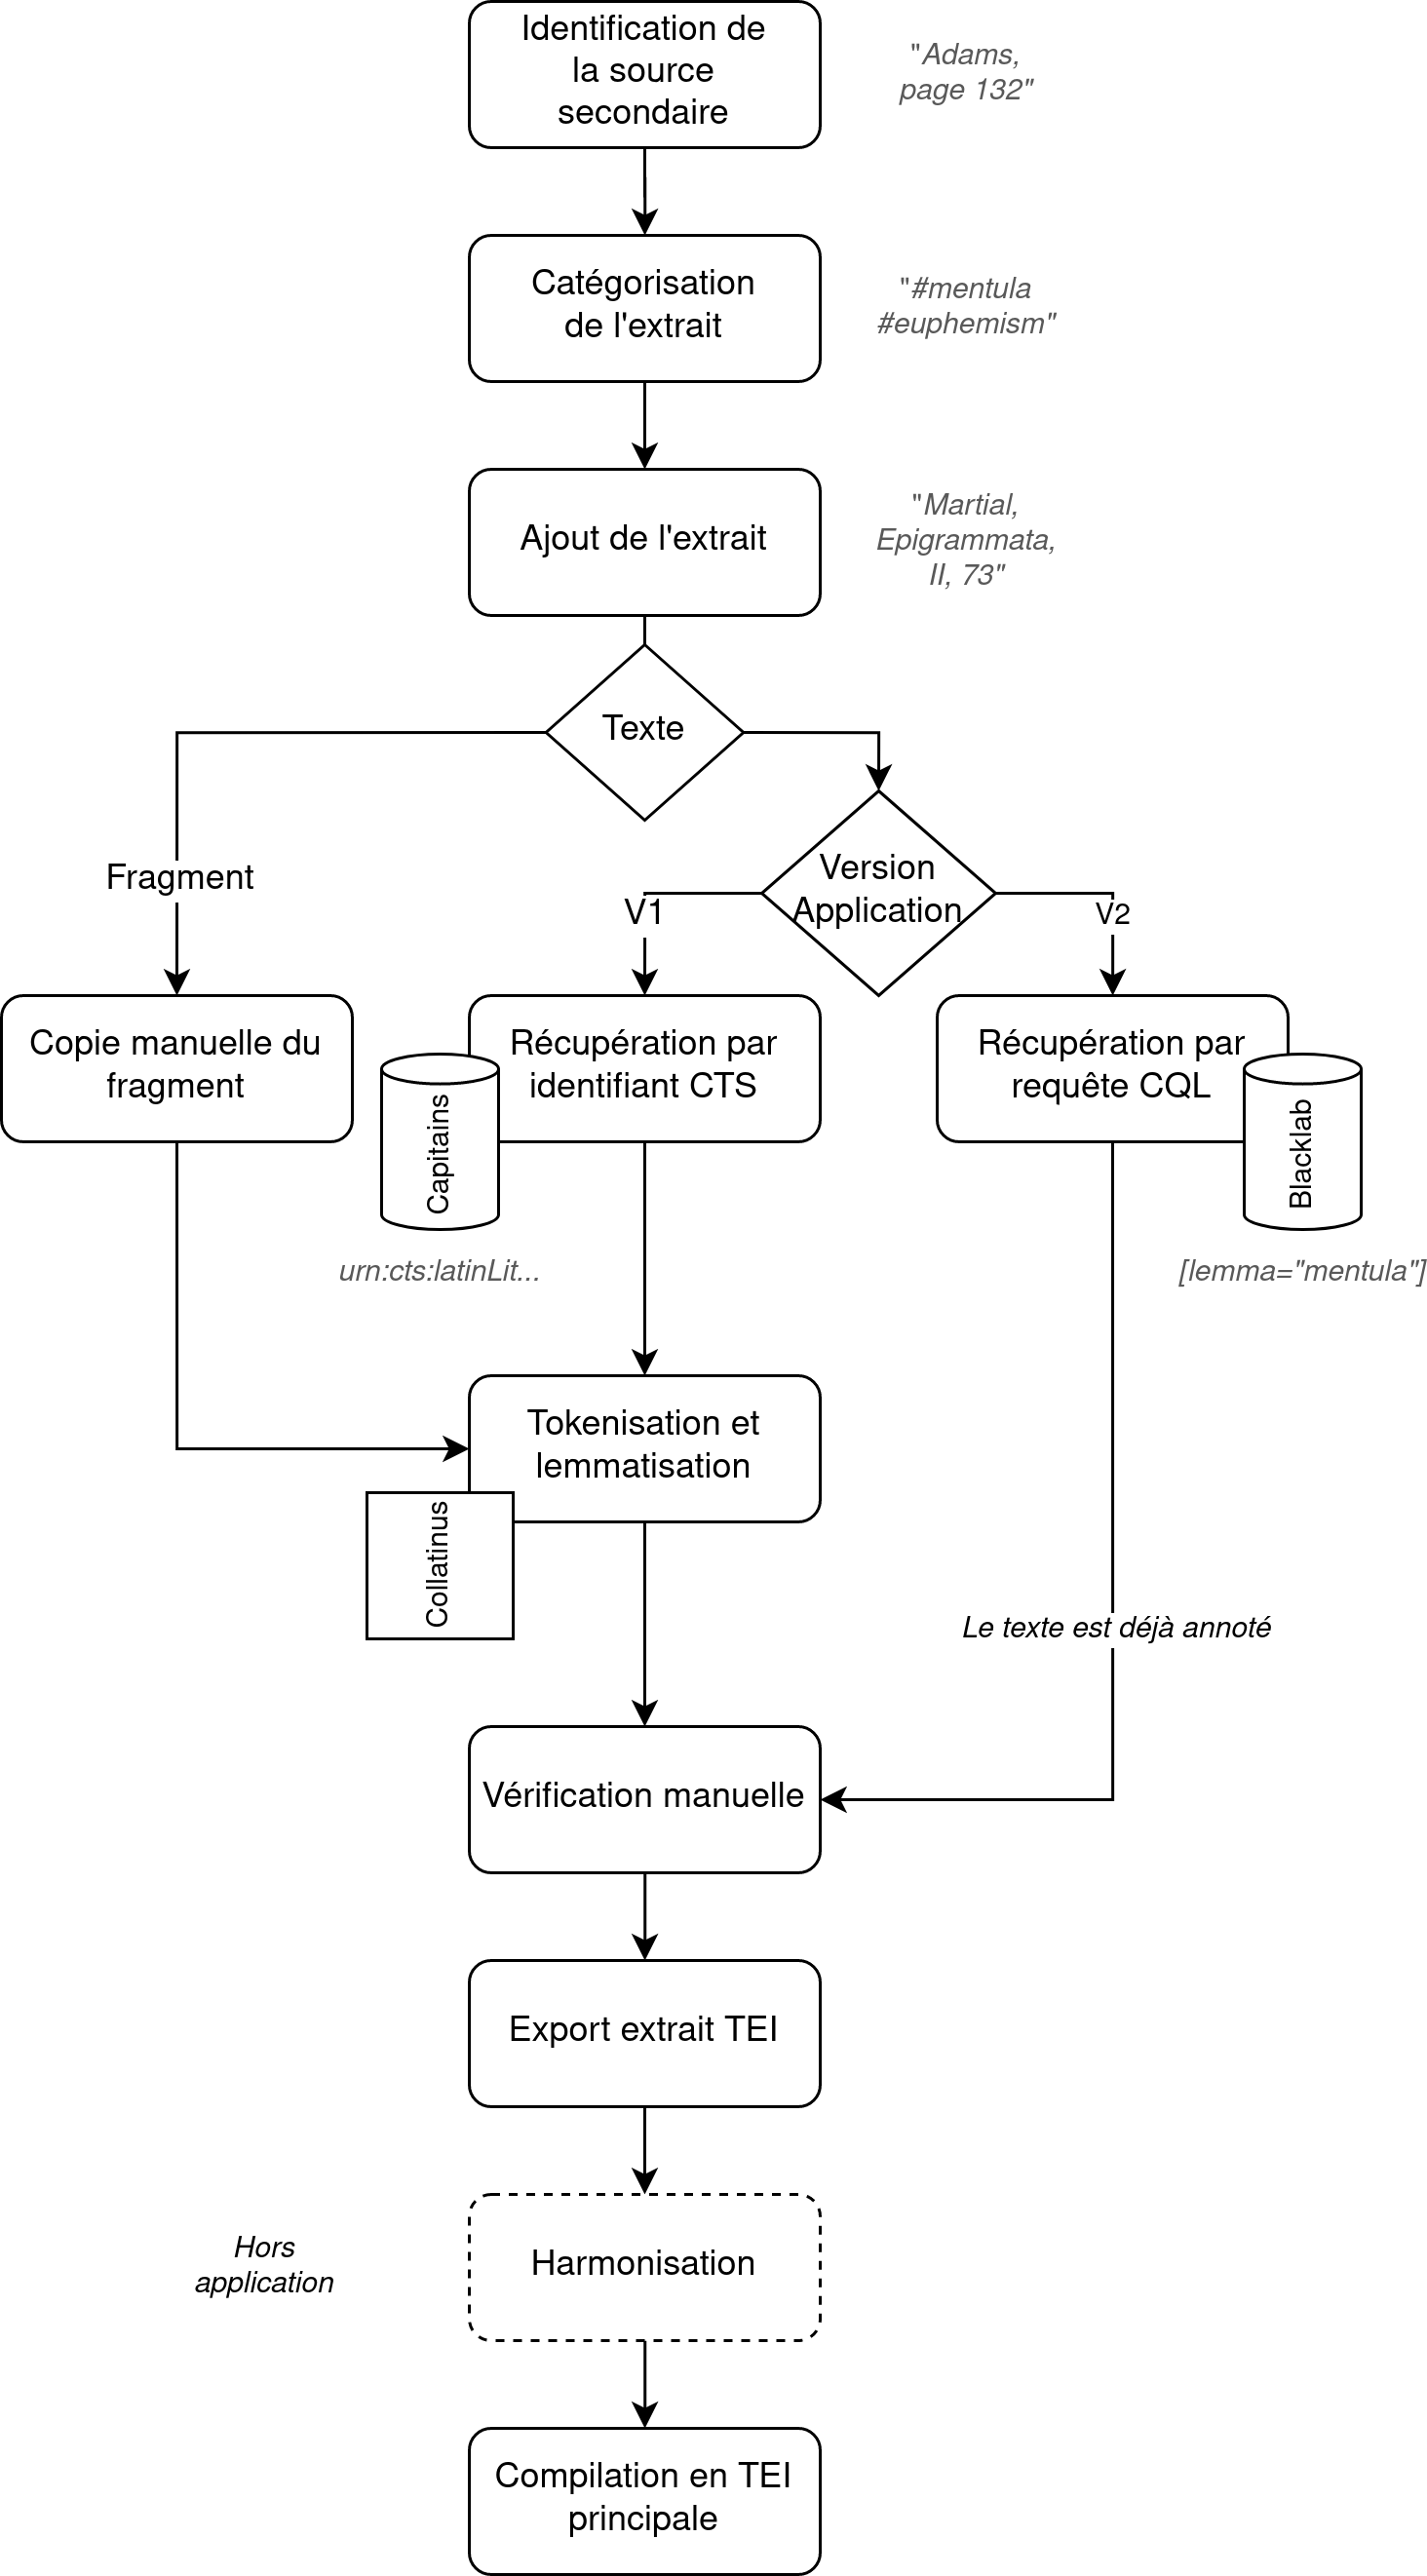
\includegraphics[width=0.6\textwidth]{figures/chap1/part3/exemplier/corpus_builder_workflow.png}
    \caption{Étapes et source des données ou annotations dans le processus de création d'exemples.}
    \label{fig:chap1:corpus_builder_workflow}
\end{figure}

Les versions successives de l'application, nommée \textit{Corpus Builder}, commencent par demander à l'utilisateur d'entrer des métadonnées concernant la source secondaire justifiant l'intégration de l'extrait: Adams et, le cas échéant, le TLL (\textit{cf.} figure \ref{fig:chap1:corpus_builder_workflow}). Une fois ces informations bibliographiques remplies, la deuxième étape consiste à ajouter ou à sélectionner des catégories, utilisées comme mots clefs. Il est possible de les choisir à partir d'une liste prédéfinie de \textit{tags} importants, de reprendre ceux retrouvés dans les extraits déjà annotés ou bien d'en ajouter de nouveaux. Une de ces annotations sort du lot: \enquote{composite} permet d'indiquer que le sens sexuel est obtenu à travers la combinaison de deux mots ou plus, par exemple \textit{cum + \_ + esse} (être avec quelqu'un)\footnote{Exemple 1466: \enquote{\textit{Quid ego tibi deliqui, si, cui nupta sum, tecum {tecum} fui ?}} \textcite[p.~177]{adams}.}. Ces deux étapes permettent de préparer le document à produire du point de vue de ses métadonnées.

\begin{figure}
    \centering
    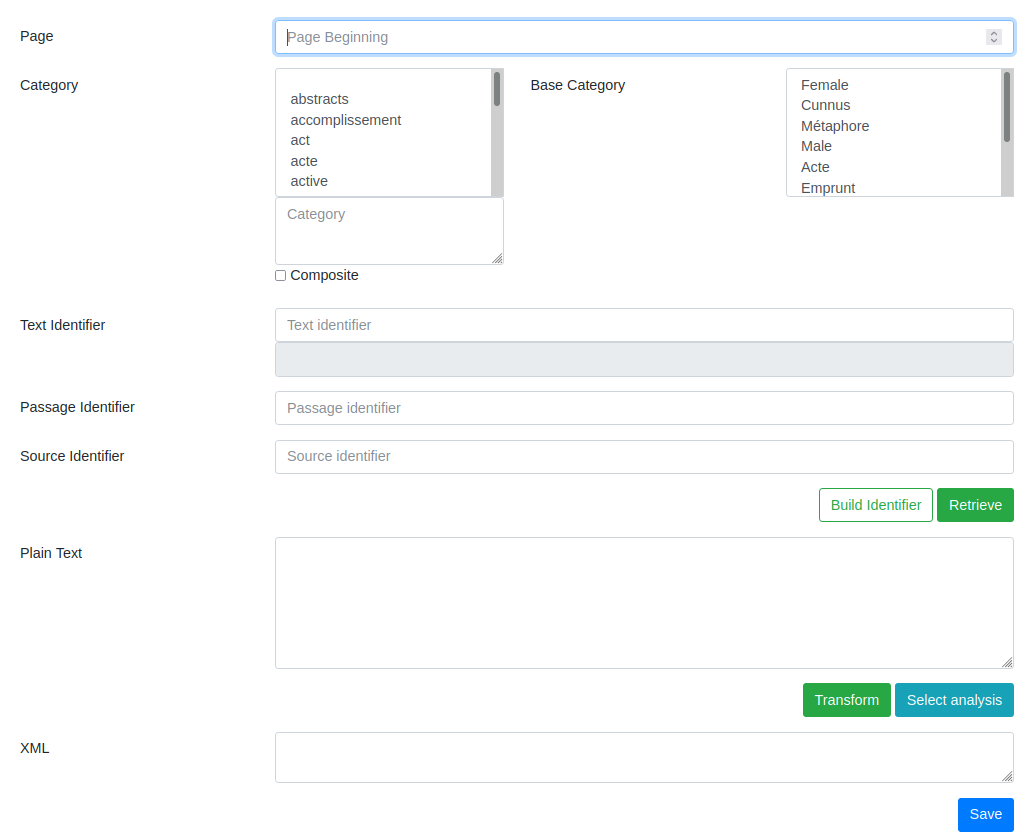
\includegraphics[width=\textwidth]{figures/chap1/part3/exemplier/corpus_builder_single.png}
    \caption{Page de l'application \textit{Corpus Builder} pour un passage unique.}
    \label{fig:chap1:corpus_builder_single}
\end{figure}

La première version de l'application (Figure \ref{fig:chap1:corpus_builder_single}), ne contenait qu'un simple système permettant soit de récupérer le texte à partir d'un identifiant CTS dans la base du meta-corpus, soit de fournir un texte \enquote{nu}, par exemple pour les fragments absents de notre compilation, en tapant directement le texte dans l'interface. Le texte est alors accompagné de métadonnées fournies par l'utilisateur: identifiant de l'œuvre, voire de l'édition, et identifiant du passage. Une fois le texte obtenu ou copié, il est découpé en \enquote{mots}, via des règles extrêmement simples (ponctuations et espaces), et envoyées à la lemmatisation et à l'analyse morphologique à une version python de collatinus. Une fois l'analyse effectuée, une version temporaire du XML est présentée à l'utilisateur, qui peut sélectionner le ou les mots qui portent l'analyse fournie par Adams, afin de porter au niveau mot l'interprétation d'Adams via l'attribut \texttt{@ana}. L'utilisateur peut ensuite sauvegarder le document.

\begin{figure}
    \centering
    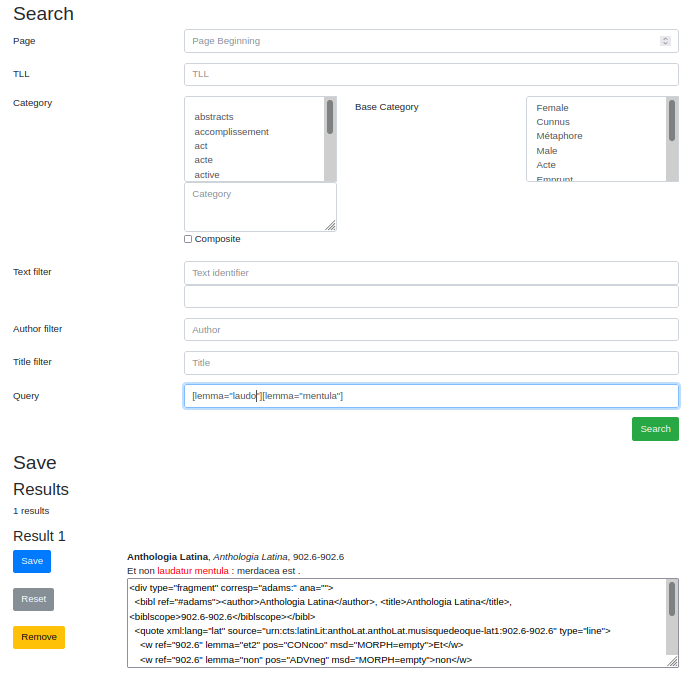
\includegraphics[width=\textwidth]{figures/chap1/part3/exemplier/corpus_builder_multiple.png}
    \caption{Page de l'application \textit{Corpus Builder} pour de multiples passages.}
    \label{fig:chap1:corpus_builder_mult}
\end{figure}

La seconde version de l'application ajoute une page de recherche multiple (Figure \ref{fig:chap1:corpus_builder_mult}). Elle repose sur une version du corpus ingérée par le moteur de recherche linguistique Blacklab\footcite{de2017creating} qui propose une interface machine (API) acceptant les requêtes utilisant le \acrfull{CQL}. Le \acrshort{CQL}\footcite{christ1994modular} est un langage de requêtage permettant de chercher des informations sur des annotations au niveau mot. Notre meta-corpus est proposé dans ce moteur de recherche sous une forme favorisant des recherches avancées (\textit{cf.} figure \ref{fig:chap1:armavirumque}): chaque mot est accompagné d'une part des annotations issues de l'extraction de données -- comme la structuration logique et la référence canonique du passage -- et d'autre part d'annotations automatiques effectuées par le lemmatiseur Pie\footnote{\textit{Cf. Chapitre 3.}}, incluant le lemme, la POS, la morphologie. On peut alors produire des requêtes complexes, s'appuyant à la fois sur les informations bibliographiques (à travers les filtres Auteur ou œuvre par exemple, mais aussi les filtres au niveau mot pour les passages) et sur les informations linguistiques issues de l'annotation automatique. Cette deuxième version a permis une nette accélération dans la constitution du corpus: il devenait possible d'annoter, après vérification manuelle, des dizaines d'extraits à travers une seule recherche \enquote{complexe}. Cette option est devenue d'autant plus pratique pour les situations où Adams, par manque d'espace, se contente de dire qu'il y a \textit{X} occurrences d'un certain lemme chez un ou plusieurs auteurs nommés.

\begin{figure}
    \begin{lstlisting}[language=XML]
<ab type="line" n="urn:cts:latinLit:phi0690.phi003.perseus-lat2:1.1">
    <w rend="line" n="1.1" pos="NOMcom" msd="Case=Acc|Numb=Plur" lemma="arma">Arma</w>
    <w rend="line" n="1.1" pos="NOMcom" msd="Case=Acc|Numb=Sing" lemma="uir">virumque</w>
    <w rend="line" n="1.1" pos="CON" msd="MORPH=empty" lemma="que">{virumque}</w>
    <w rend="line" n="1.1" pos="ADJqua" msd="Numb=Sing|Gend=MascNeut|Deg=Pos|Mood=Ind|Tense=Pres|Voice=Act|Person=1" lemma="cano">cano</w>
    <w rend="line" n="1.1" pos="PUNC" msd="MORPH=empty" lemma=",">,</w>
    \end{lstlisting}
    \caption{Premiers mots de l'\textit{Énéide} de Virgile dans le document ingéré par Blacklab.}
    \label{fig:chap1:armavirumque}
\end{figure}

La lemmatisation issue de la première version, et donc de l'outil \textit{Collatinus}\footnote{Décrit en chapitre 3.}, a été complètement reprise une fois la compilation des documents achevée. Afin de proposer une version cohérente des données pour l'apprentissage machine, chaque mot a été annoté par le même lemmatiseur que celui utilisé pour le meta-corpus dans Blacklab, ajoutant ainsi un lemme, une POS et une analyse morpho-syntaxique. Enfin, les mots-clefs dérivés des catégories d'Adams ont été harmonisés, semi-automatiquement: les listes n'étaient pas assez contraignantes et des variations orthographiques s'y étaient glissées. Nettoyer ces données a permis ainsi d'optimiser l'opérabilité de ces dernières dans un exemplier présentant, désormais, une bonne cohérence interne.

% Interpréter Adams: le problème des tags ?
% Notes sur quelques données absentes

\subsubsection{Produit final: navigation et analyse quantitative}

Après avoir produit un meta-corpus important et finement structuré, nous avons pu construire, à travers un ensemble d'outils que nous avons précédemment présentés, un exemplier numérique. Nous proposons, avant d'aller plus loin dans le traitement numérique de cet exemplier (Chapitre 5), de le décrire. Nous présenterons ensuite les prémices d'une interface permettant de valoriser ce nouvel objet numérique.

\paragraph{Caractéristiques statistiques de l'exemplier}

L'exemplier produit est assez important\footnote{Il n'existe pas à notre connaissance de bases de ce type de disponible.}: deux mille cinq cent seize exemples le composent. Il comprend 38~201 mots (hors ponctuation) répartis entre quatre-vingt-dix-sept auteurs. Il est accompagné de cent quatre-vingt-dix-neuf mot-clefs (qui représentent, entre autres, les catégories), utilisés dans huit mille deux cent quinze annotations pour trois cent quarante-deux combinaisons uniques. Le set de données s'étend de Plaute (-254) à Pierre Diacre (1159): le texte de ce dernier a été inclus suite à une erreur de datation. L'auteur du XII\textsuperscript{e} siècle exclu, la date la plus tardive devient celle du premier Mythographe du Vatican. Ce dernier a été daté pendant longtemps autour des V\textsuperscript{e} et VI\textsuperscript{e}, ce qui justifie son inclusion, mais cette datation est fortement remise en cause dans sa dernière édition de 1995\footnote{Plus de dix ans après la publication d'Adams. La datation nous est donnée par une citation dans le projet DigilibLT: \textcite{zorzetti_premier_1995}.}, où Nevio Zorzetti et Jacques Berlioz proposent une datation entre le VIII\textsuperscript{e} et le IX\textsuperscript{e} siècle.

\begin{figure}
    \centering
    \begin{minipage}[b]{.48\linewidth}%
        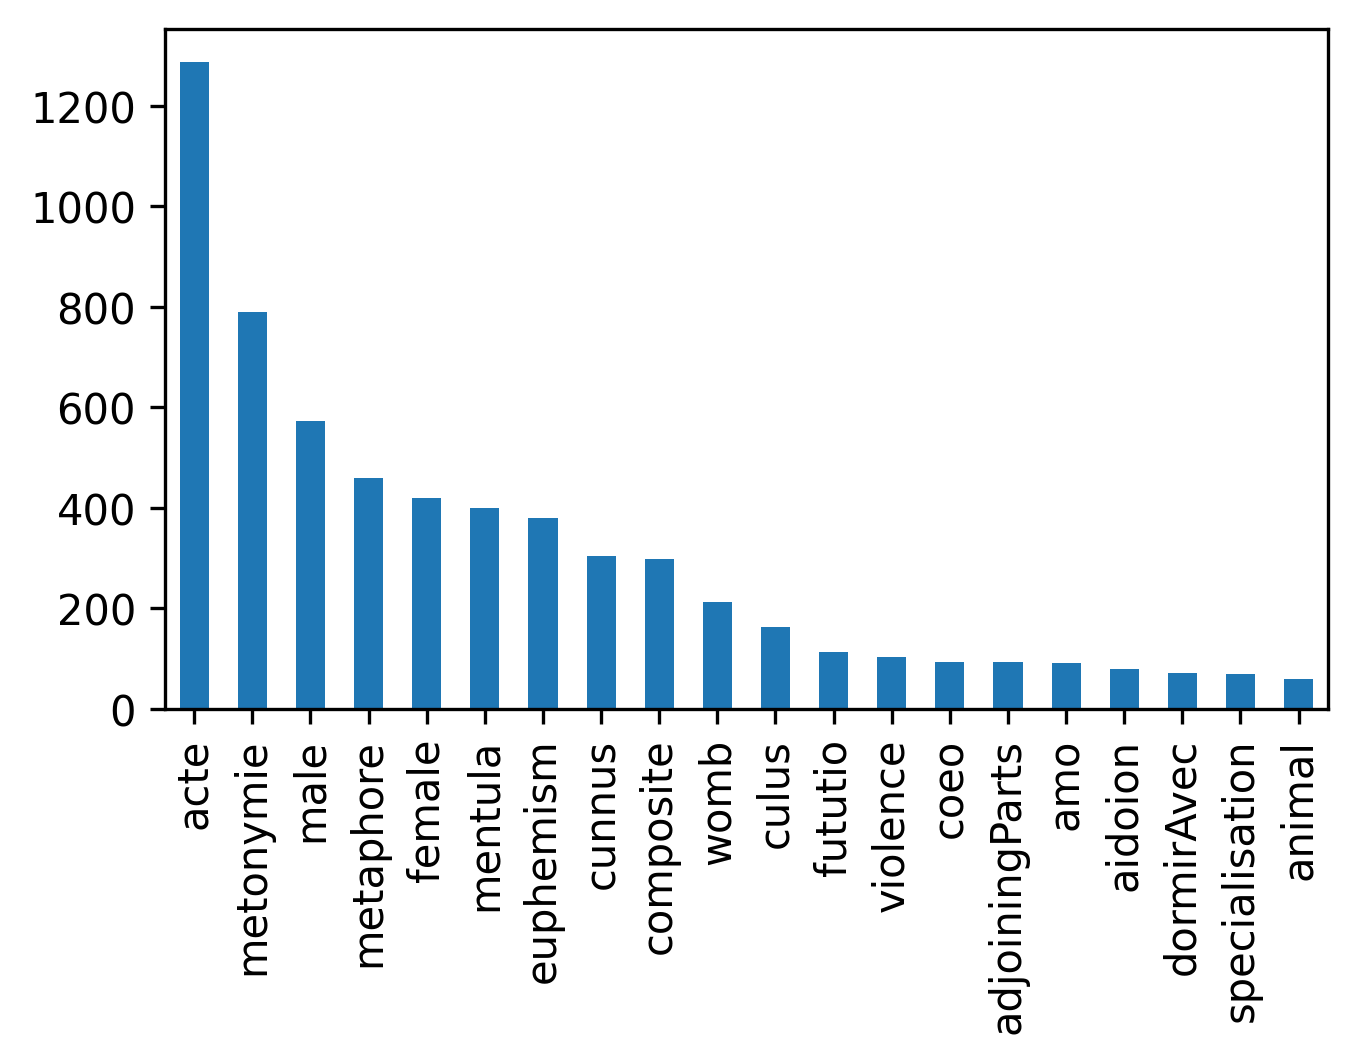
\includegraphics[width=\linewidth]{figures/chap1/part3/exemplier/tags.png}
        \caption{Vingt tags les plus fréquents de l'exemplier}
        \label{fig:chap1:tag_mostfrequents}
    \end{minipage}
    \hfill
    \begin{minipage}[b]{.48\linewidth}%
        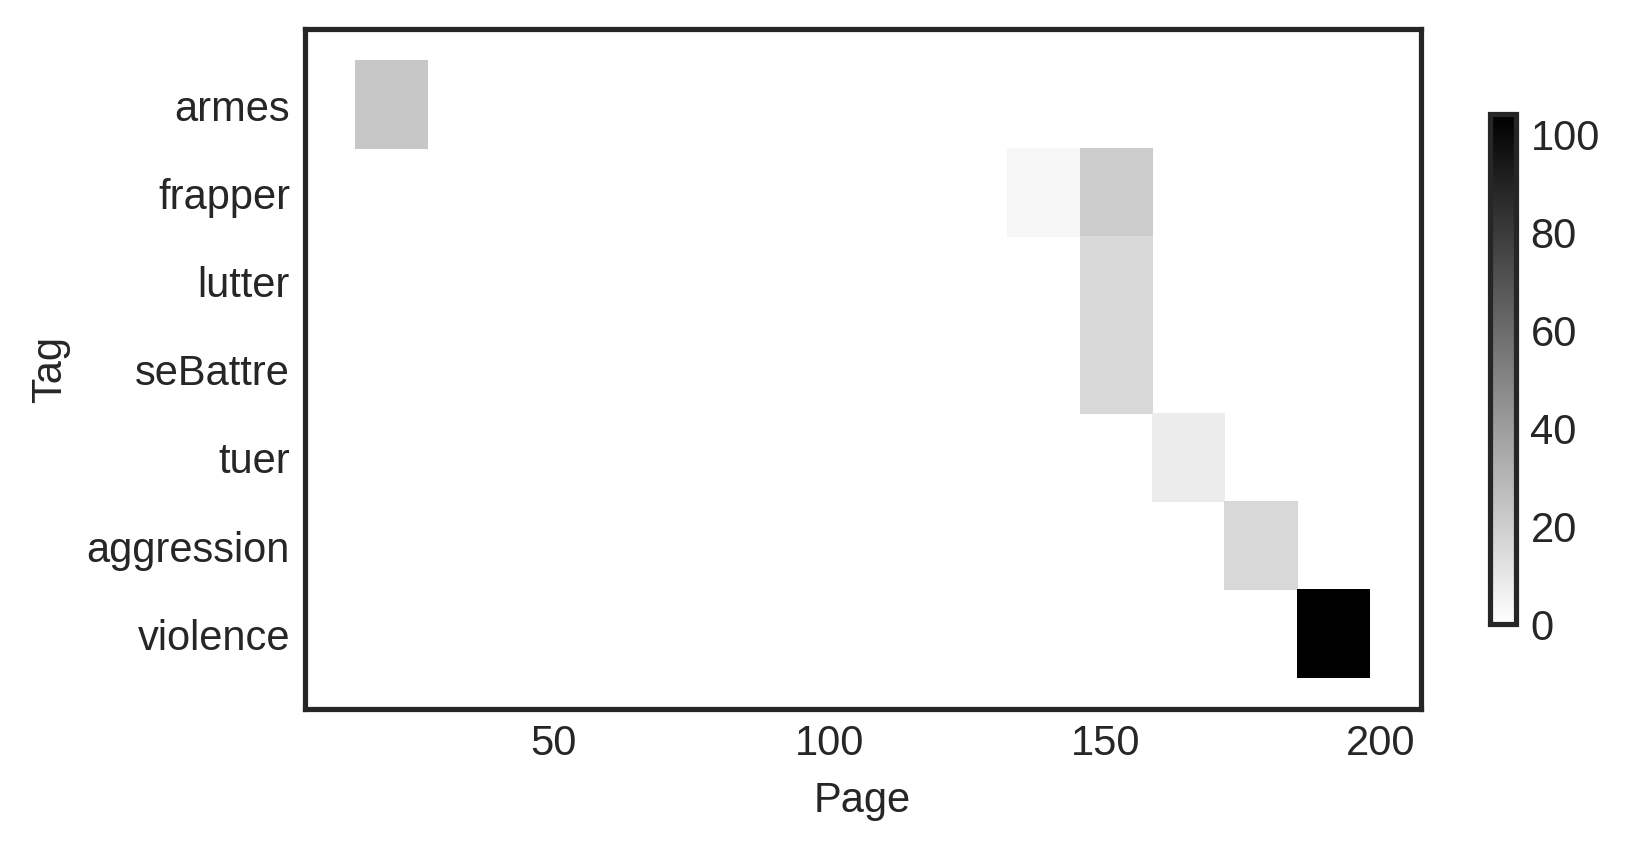
\includegraphics[width=\linewidth]{figures/chap1/part3/exemplier/violence.png}
        \caption{Fréquence des tags liés à la violence}
        \label{fig:chap1:tags_violence}
    \end{minipage}
\end{figure}

Les annotations catégorielles les plus communes sont sans surprise les catégories principales d'Adams, avec d'une part les catégories \enquote{thématiques} (ses chapitres: acte, \textit{male} pour sexe masculin, \textit{female} pour sexe féminin, \textit{culus}) et ses outils d'analyse intra thématiques (\textit{metaphore}, \textit{metonymie)}. En figure \ref{fig:chap1:tag_mostfrequents}, les vingt \textit{tags} les plus fréquents réservent tout de même quelques surprises, notamment \enquote{animal} qui recouvre métaphores animales ou vocabulaire appliqué aux animaux et qui informe soit d'une meilleure connaissance de ces types d'usage chez Adams, soit d'un goût romain pour ceux-ci.

Cette visualisation met en exergue les aspects critiquables de ces catégorisations\footnote{Si cette erreur de méthode ne met pas en valeur notre travail, il nous semble capital d'en informer les différents utilisateurs, car elle pourrait bien induire des erreurs d'interprétations.}. Par exemple, le mot clef \enquote{violence} a été utilisé lorsqu'Adams a spécifié clairement qu'un terme ou ensemble de termes était \enquote{violents}. Si l'on regarde la figure \ref{fig:chap1:tags_violence}, il est clair que notre lecture linéaire d'Adams, sans avoir su en amont l'ensemble des qualifications qu'il utilise, a produit en aval des traitements différenciés de ces dernières. C'est une faiblesse notable de l'usage des catégorisations, en dehors des catégories extrêmement claires de l'auteur lui-même (type \enquote{acte} et \enquote{métaphores}). En cas d'introduction d'exemples à travers d'autres sources secondaires comme celles d'Amy Richlin, il sera nécessaire de lisser ces catégories et de décrire le thésaurus qui permet ce classement. Cette stabilisation ontologique devrait s'accompagner de son approfondissement, par exemple en incluant une meilleure qualification des personnes impliquées dans les scènes sexuelles. Des catégories telles que \texttt{\#Actif:Homme}, \texttt{\#Actif:Esclave}, etc. permettraient, y compris à travers des approches modernes et potentiellement anachroniques, de réinterroger ces dernières et de profiter un peu plus à l'histoire en plus d'apporter beaucoup à la lexicographie.

\begin{figure}[ht]
    \centering
    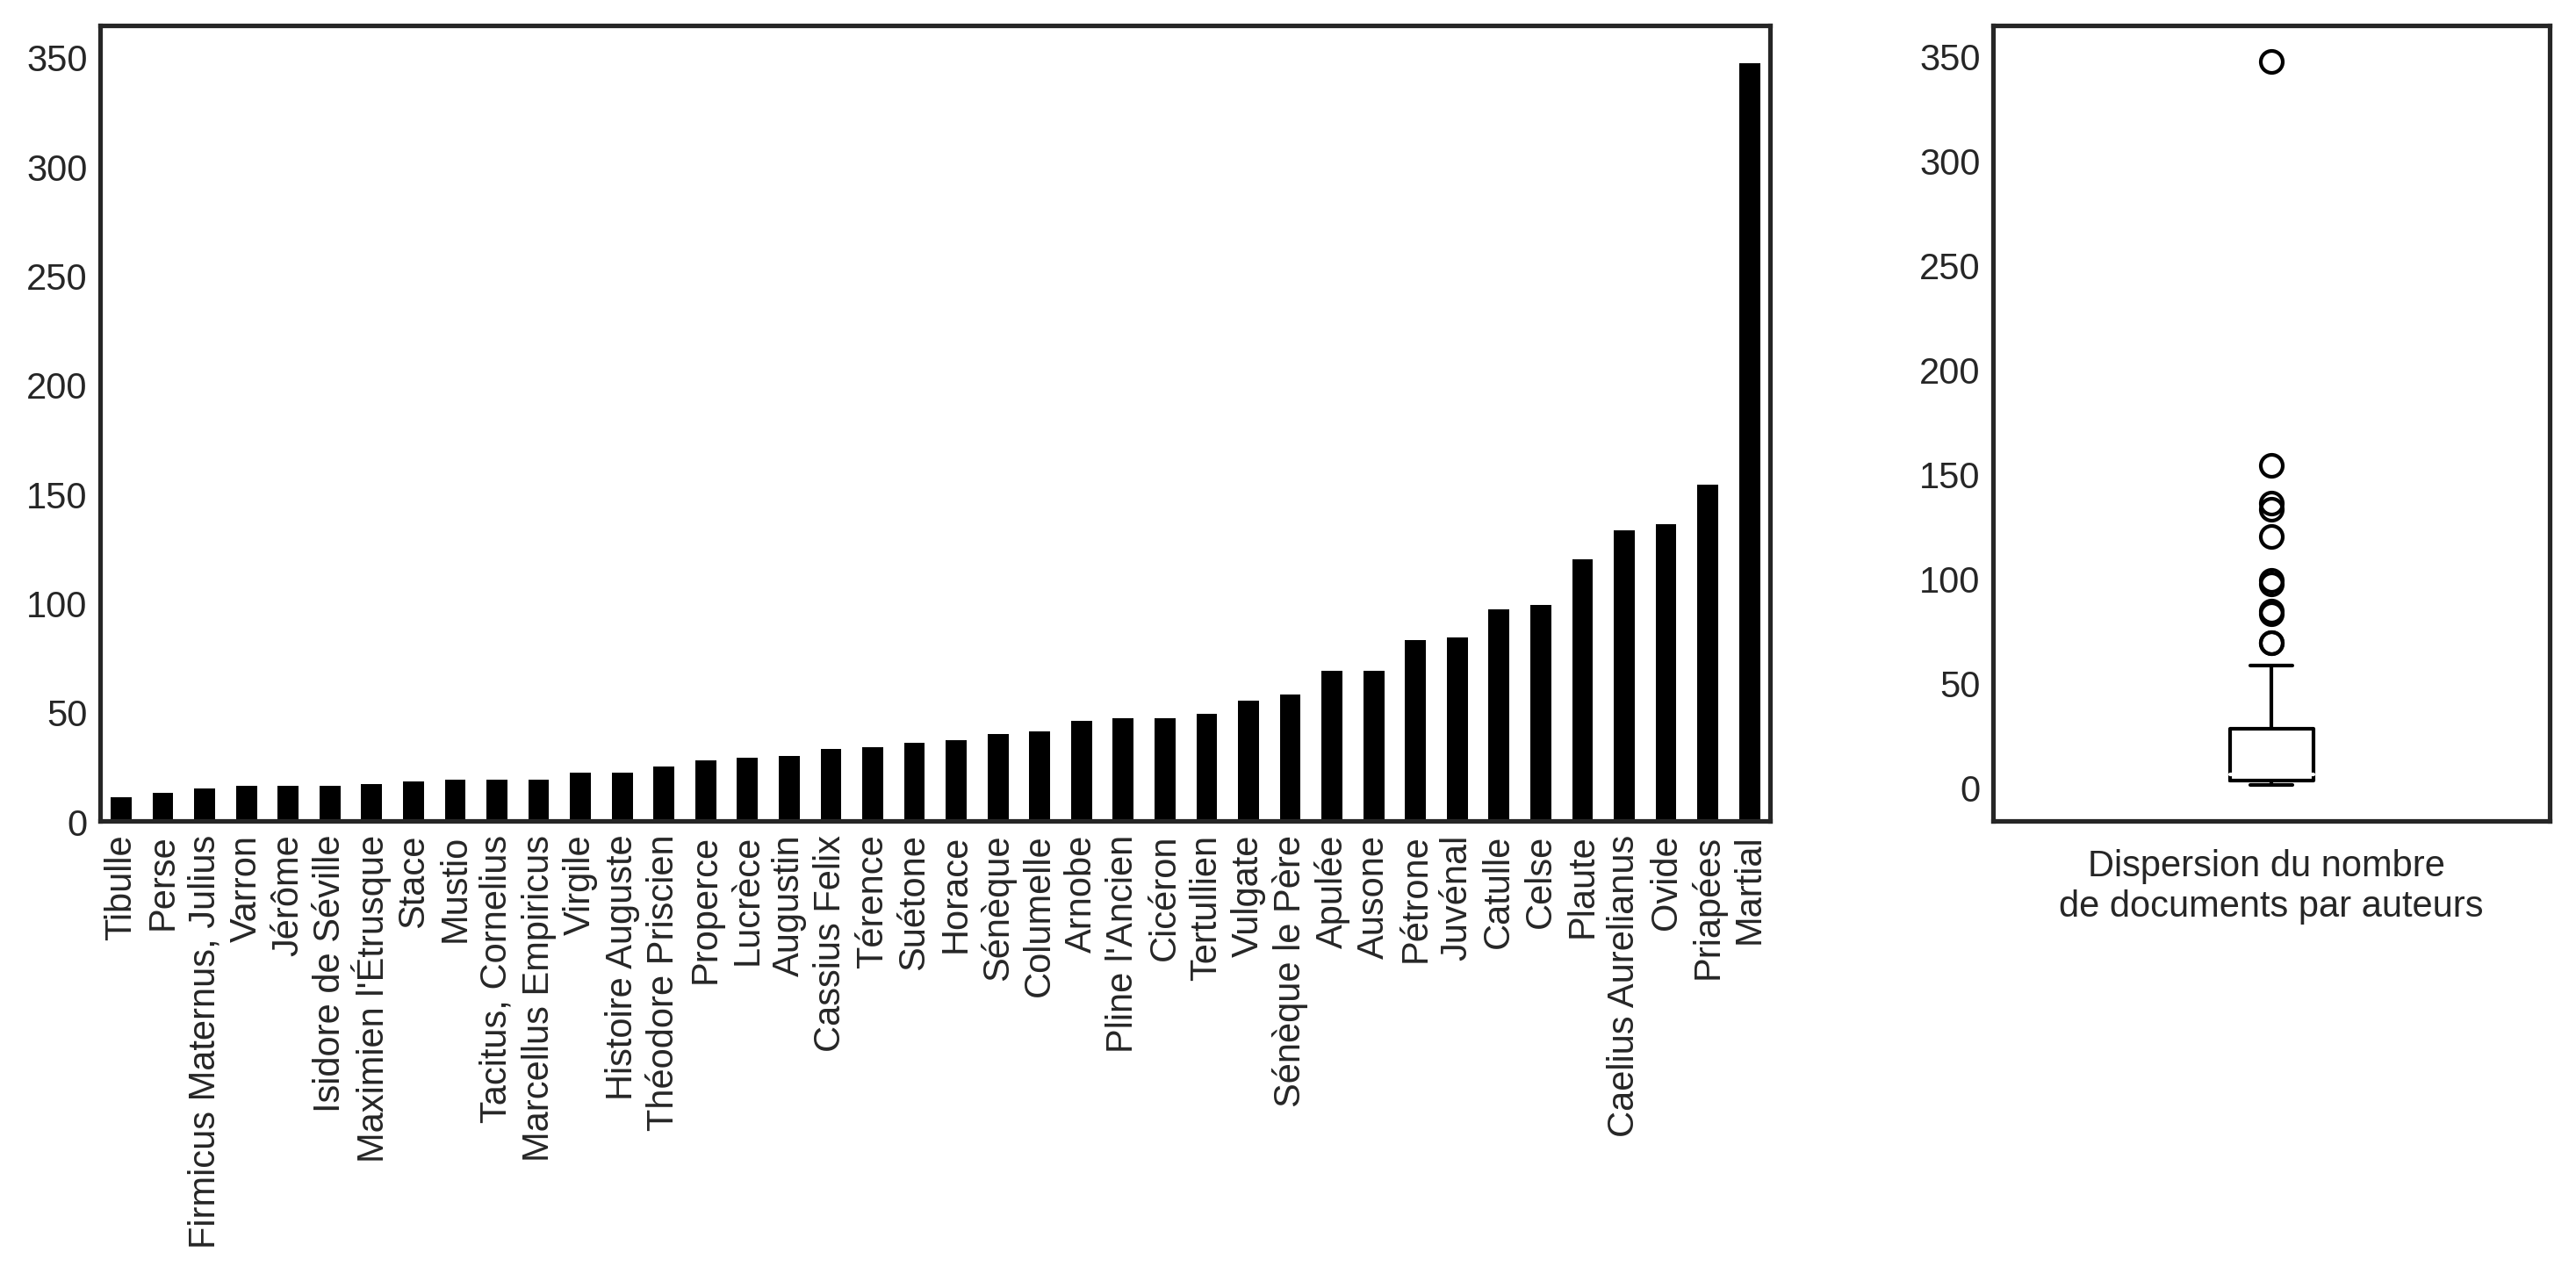
\includegraphics[width=\linewidth]{figures/chap1/part3/exemplier/auteurs_exemplier_absolus.png}
    \caption{Auteurs les plus importants en nombre d'exemples.}
    \label{fig:chap1:nb_extraits_auteur}
    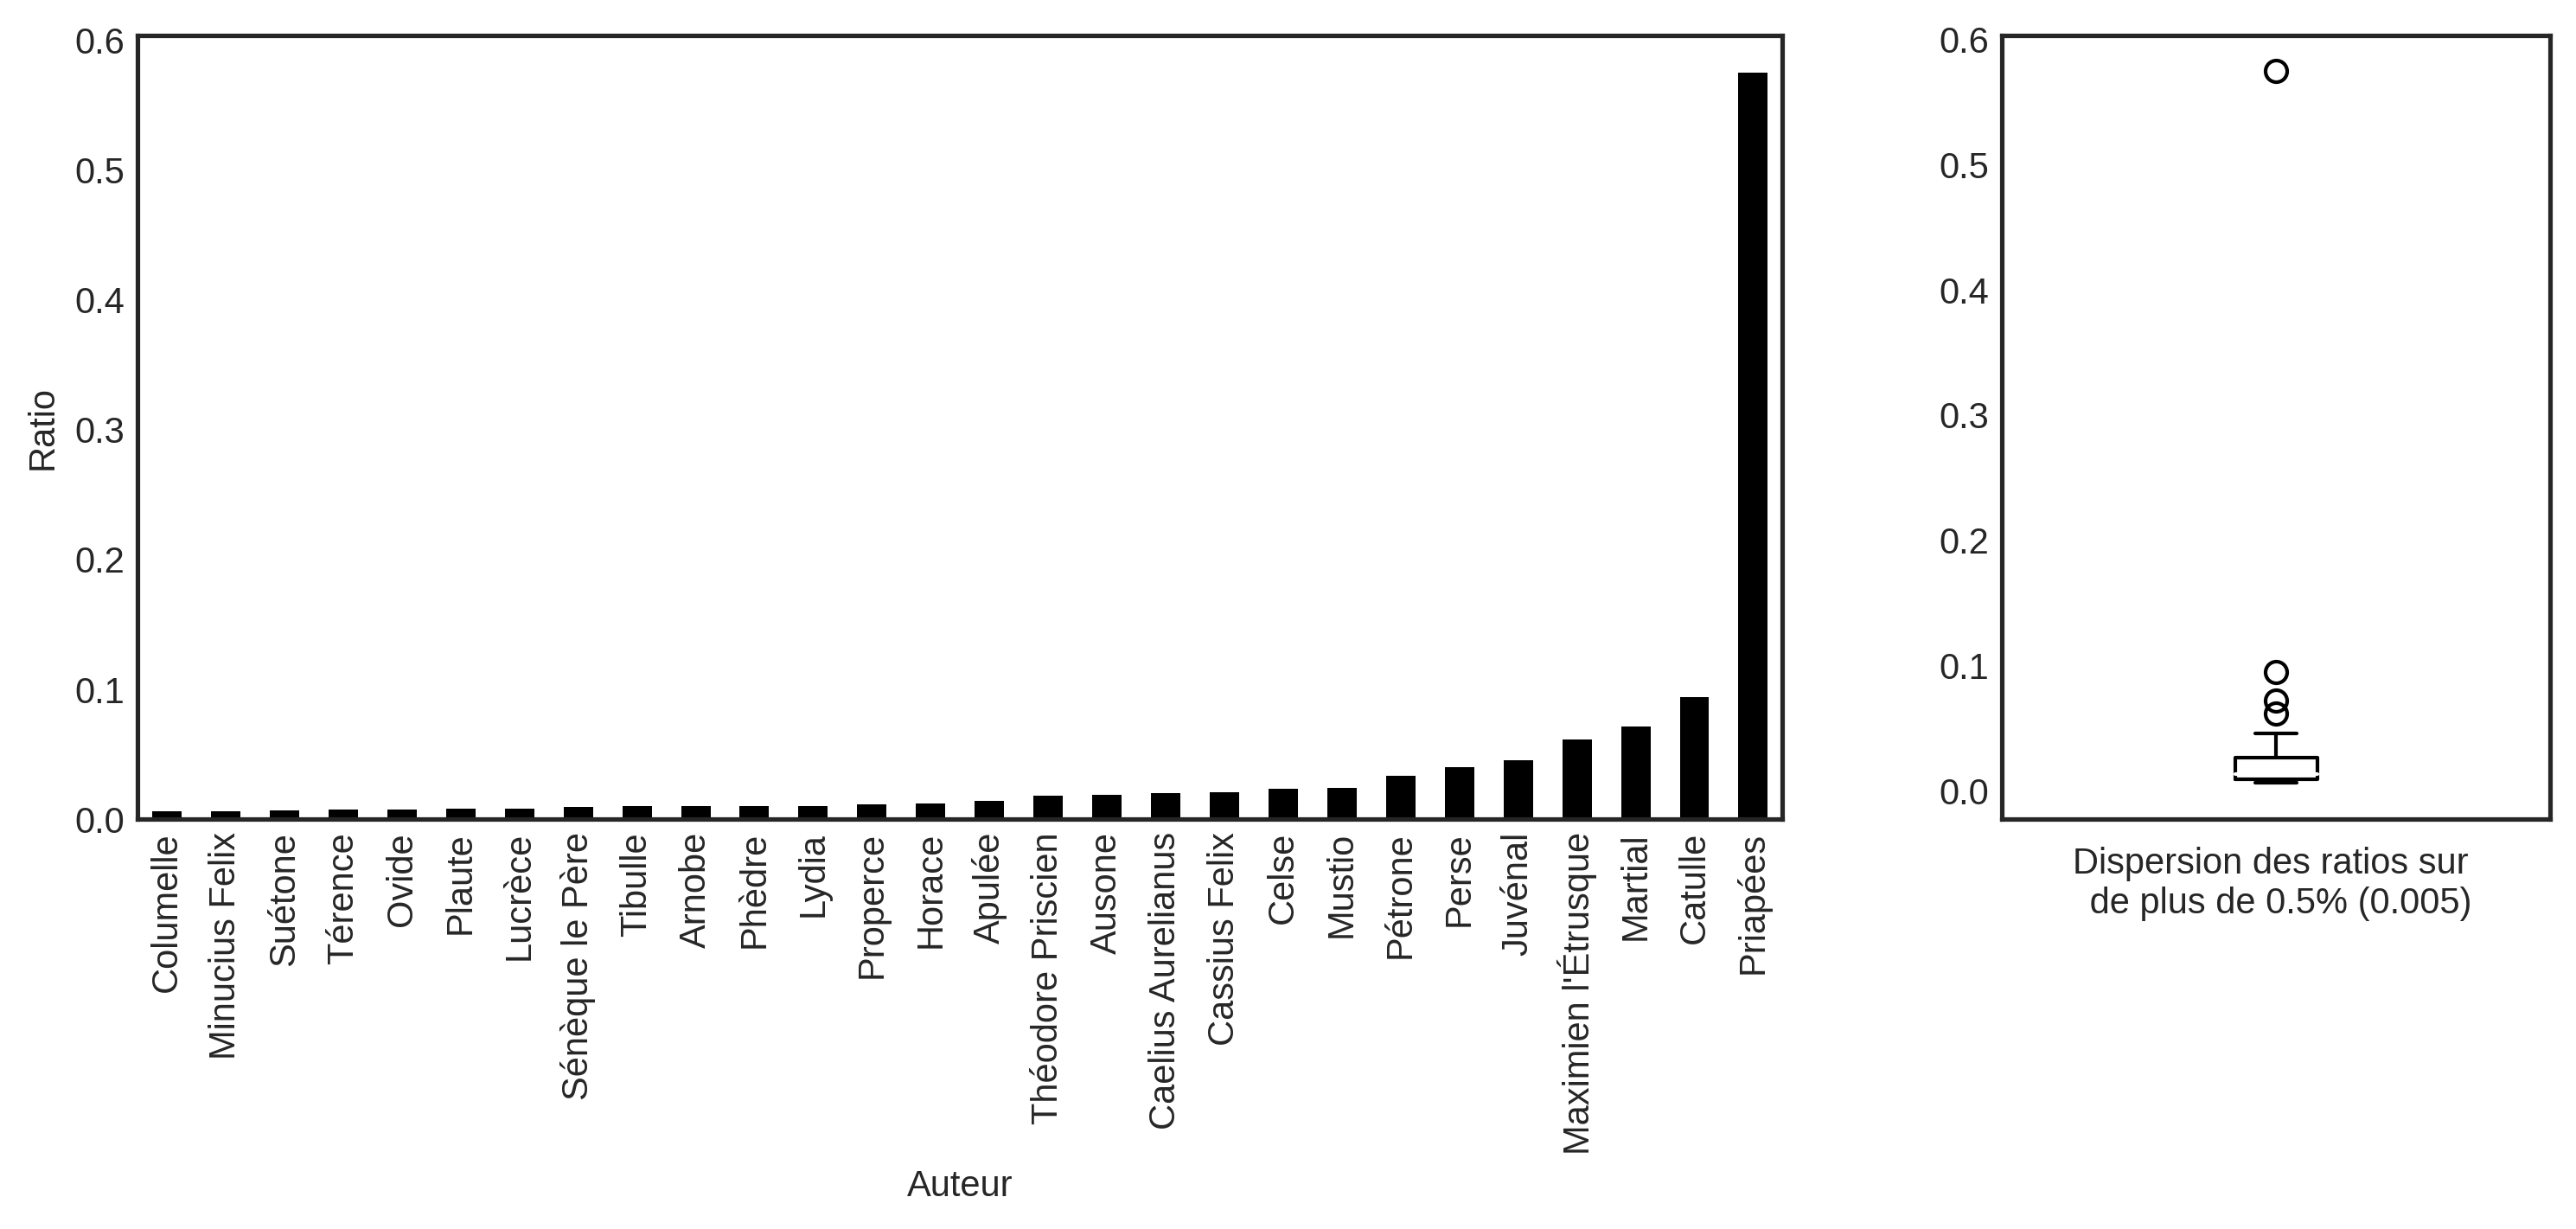
\includegraphics[width=\linewidth]{figures/chap1/part3/exemplier/auteurs_exemplier_motsrelatifs.png}
    \caption{Auteurs les plus importants en fonction du ratio Nombre de mots dans l'exemplier par nombre de mots dans le meta-corpus.}
    \label{fig:chap1:nb_extraits_auteur_rel}
\end{figure}

La distribution des exemples en fonction de leur auteur ou de la compilation qui les contient montre une distribution de Paretto (peu d'auteurs sont extrêmement riches en exemples) due majoritairement à des différences génériques. Les auteurs les plus importants du corpus en nombre d'exemples sont des poètes (Ovide, Catulle, Martial, etc.), des médecins ou \enquote{scientifiques} (Caellius Aurelianus, Celse) ou des auteurs de comédie (Plaute). Martial est en valeur absolue l'auteur le plus prolifique d'exemple dans notre corpus: son langage fleuri et les thèmes qu'il aborde en font un auteur incontournable pour la compréhension de la sexualité latine. Ce décompte, mis en regard de la taille de l'œuvre de chaque auteur (\textit{cf.} figure \ref{fig:chap1:nb_extraits_auteur_rel}), permet aussi de détecter les auteurs dont la sexualité est un terme central. En rapportant le nombre de mots dans les extraits issus de son œuvre au nombre de mots dans les exemples cités chez Adams, Catulle passe de la septième à la deuxième place dans le classement des auteurs les plus importants. Cela signifie que, comparé à Martial, Catulle parle plus souvent de sexualité pour chaque mot qu'il écrit. Ces chiffres montrent aussi la spécificité de l'écriture des \textit{Priapées}, avec plus d'un mot sur deux écrits repris dans l'exemplier. Ils soulignent aussi celle des médecins ou gynécologues comme Celse ou Mustio, qui se glissent dans les dix auteurs les plus prolifiques sur cette thématique. Enfin, il met en lumière des phénomènes de transmission, comme pour Maximien l'Étrusque, que l'on ne connait que pour six élégies, et qui, mécaniquement, se retrouve en haut des scores (4~300~mots).

\afterpage{%
\begin{sidewaysfigure}%
    \centering
    \begin{subfigure}{0.45\hsize}
        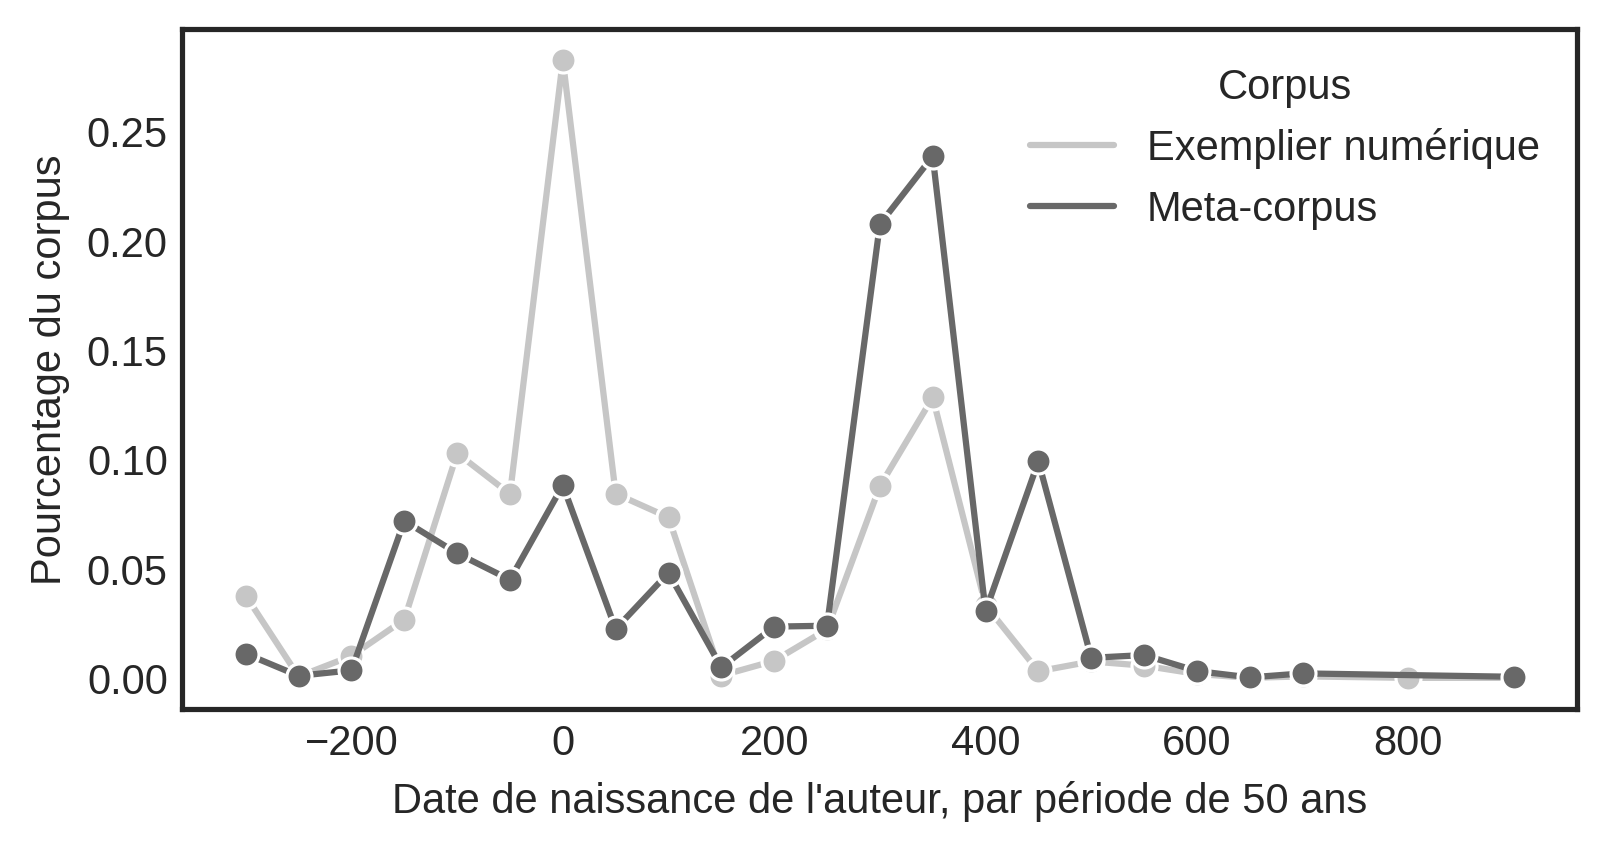
\includegraphics[width=\linewidth]{figures/chap1/part3/exemplier/evol_brut_exemplier.png}
        \caption{Répartitions des parts des corpus par date de naissance des auteurs. La période 0--50, incluant Martial, représente 25\% des extraits de l'exemplier.}
        \label{fig:chap1:exemplierdatation:brut_percent}
    \end{subfigure}%
    \hfill
    \begin{subfigure}{0.45\hsize}
        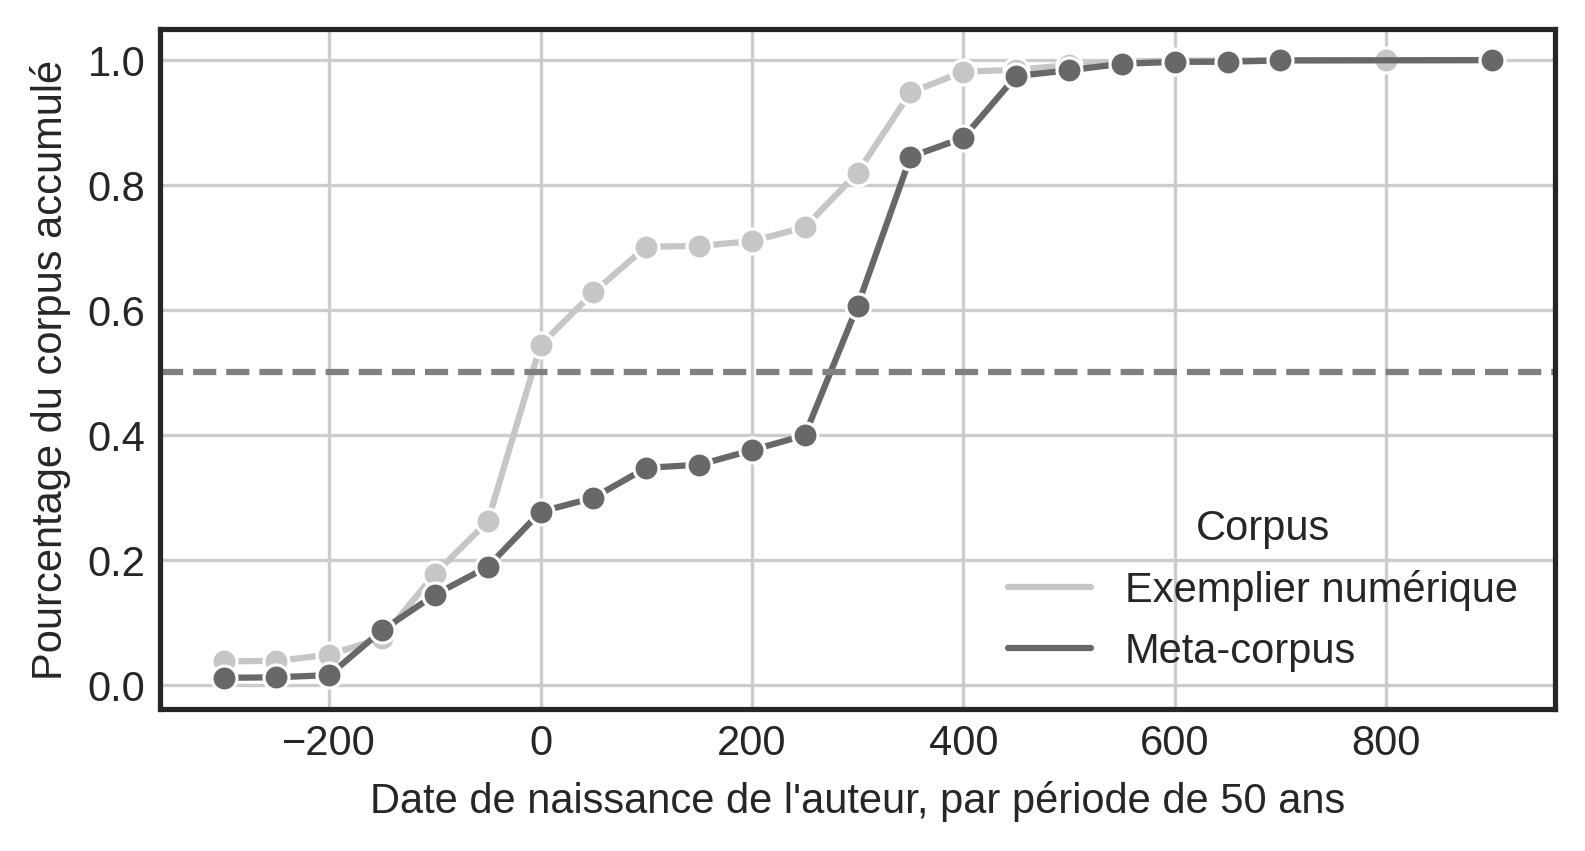
\includegraphics[width=\linewidth]{figures/chap1/part3/exemplier/evol_accumul_exemplier.png}
        \caption{Accumulation des parts des corpus par date de naissance des auteurs. La période 0--50 représente le dépassement de la barre des 50\% de l'exemplier.}
        \label{fig:chap1:exemplierdatation:accumul_percent}
    \end{subfigure}%
    \\
    \begin{subfigure}{0.45\hsize}
        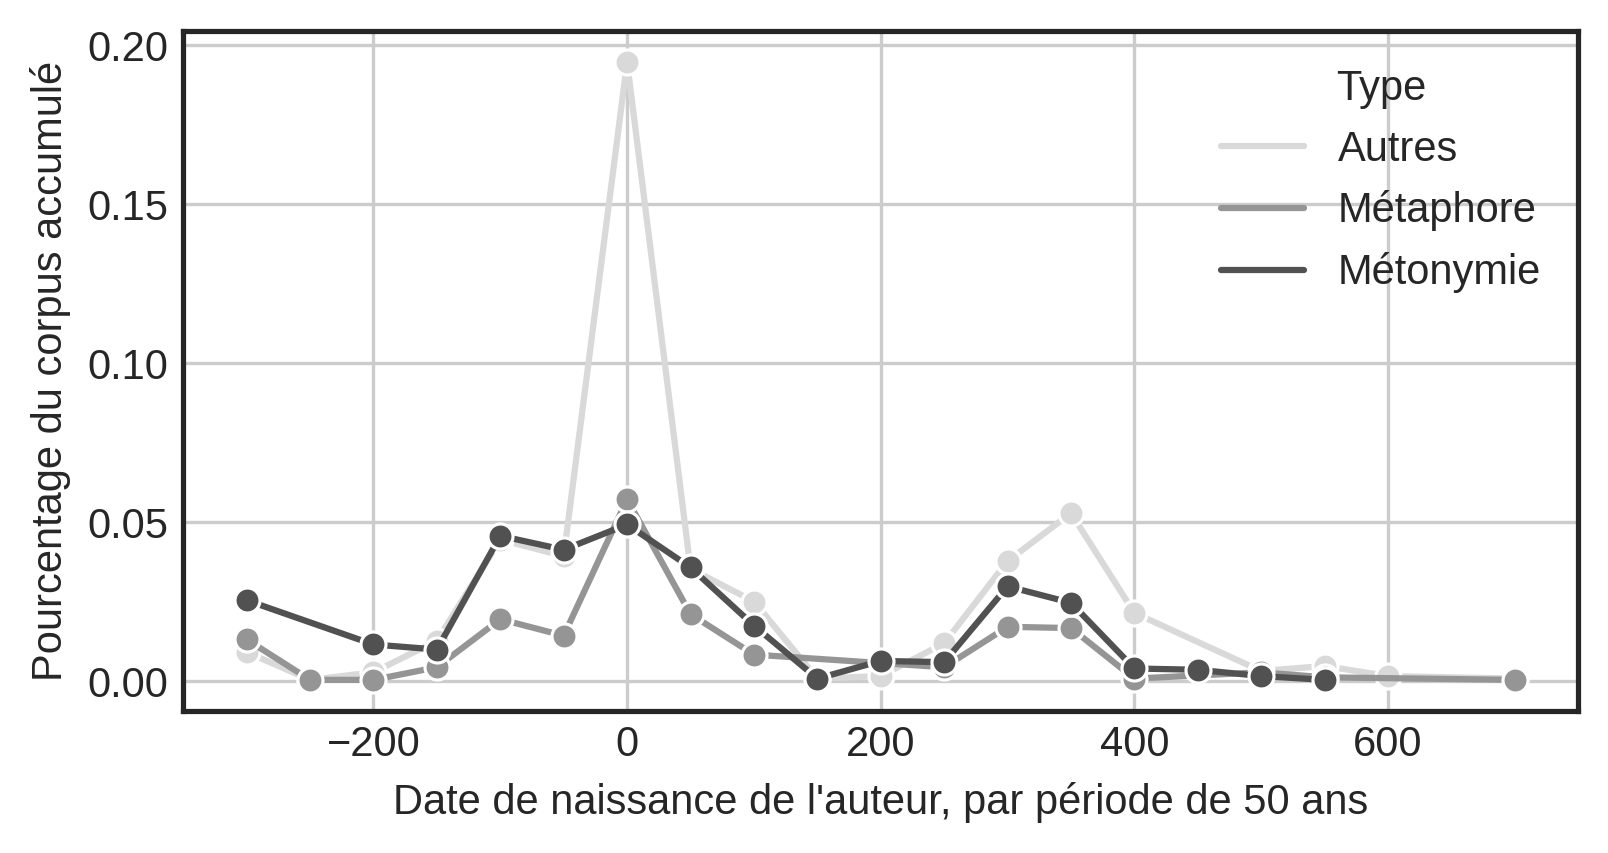
\includegraphics[width=\linewidth]{figures/chap1/part3/exemplier/evol_tags_exemplier.png}
        \caption{Répartitions des grands sous-types d'Adams (en pourcentage du corpus total) par date de naissance des auteurs. La période 0-50 a 20\% d'extraits qui ne sont ni des métaphores ni des métonymies.}
        \label{fig:chap1:exemplierdatation:tags}
    \end{subfigure}%
    \hfill
    \begin{subfigure}{0.45\hsize}
        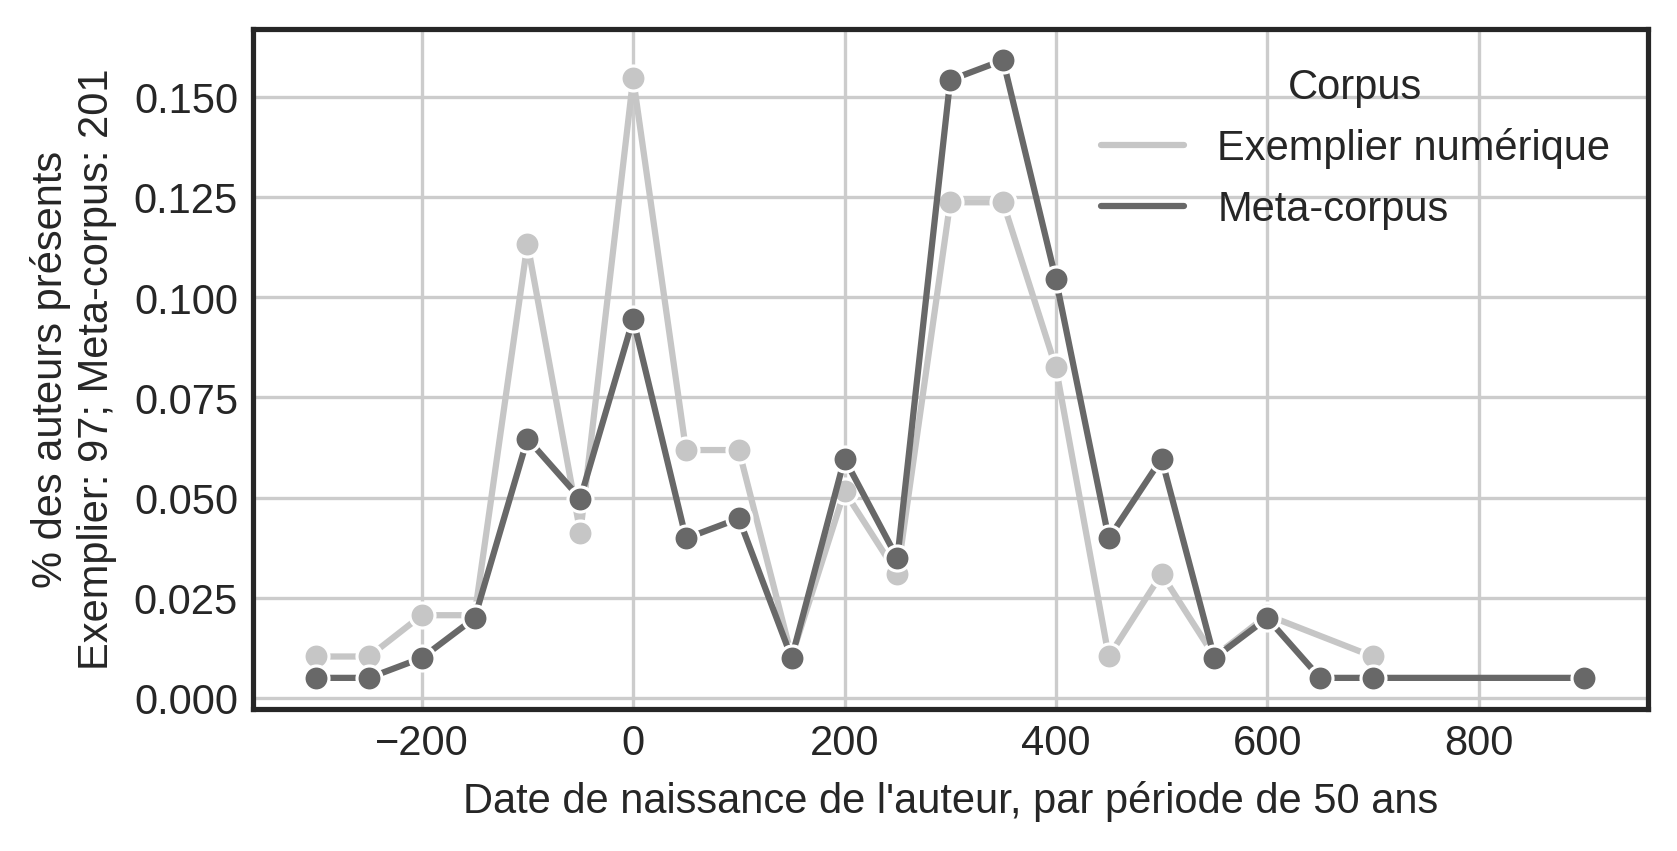
\includegraphics[width=\linewidth]{figures/chap1/part3/exemplier/evol_auteurs_exemplier.png}
        \caption{Répartitions de la portion des auteurs connus des corpus par date de naissance des auteurs. La période 0-50 contient 15\% des auteurs de l'exemplier numérique.}
        \label{fig:chap1:exemplierdatation:auteurs}
    \end{subfigure}%
    \caption{Évolution de l'exemplier en fonction de la date de naissance de l'auteur.}
    \label{fig:chap1:exemplierdatation}
\end{sidewaysfigure}%
\clearpage
}
% Chronologie

La répartition chronologique des exemples permet d'appuyer quelques points observés au sujet du méta-corpus (\textit{cf.} figure \ref{fig:chap1:exemplierdatation}). Le corpus connait deux pics chronologiques de contenus: l'un au début de l'Empire et l'un à l'apparition des œuvres des Pères latins de l'Église. Mais la force de ces pics est inversée. Quand le meta-corpus atteint son plus fort pic autour de 300 avec près de 25\% de sa couverture en nombre de mots à cette époque (\textit{cf.} figure \ref{fig:chap1:exemplierdatation:brut_percent}), l'exemplier numérique contient entre les années 0 et 50 plus de 25\% des siens. Les auteurs de l'exemplier nés entre 0 et 50 et les œuvres qui sont datées à partir de cet intervalle ne sont pas n'importe qui: Martial (Premier auteur le plus important en nombre d'exemples), Celse (Sixième), Pline l'Ancien (Seizième), l'\textit{Anthologie Latine} et les \textit{Priapées} (Deuxième). Cet écart entre période chrétienne et période classique, qui commence à se former dès la naissance des élégiaques entre -100 et 0, est clairement visible en figure \ref{fig:chap1:exemplierdatation:accumul_percent}: l'exemplier atteint la moitié de sa taille entre 0 et 50, 75\% entre 100 et 150 là où le meta-corpus n'atteint ces chiffres qu'entre 250 et 350.

Pour autant, parle-t-on moins de sexualité à la période chrétienne ? Il nous semble que deux hypothèses peuvent être avancées:
\begin{enumerate}
    \item Adams se sert beaucoup du TLL pour traiter de la période tardive et chrétienne, et le TLL pourrait avoir un traitement plus faible de cette même période. Leur couverture des textes médicaux étant imparfaite, une autre part du corpus tardif est ignoré.
    \item L'antiquité tardive ne parle pas ou plus de sexe, ou autrement, soit par changement générique (moins de satires, moins de poésie érotique), soit par sélection dans la transmission des textes.
\end{enumerate}

Il s'agit plus que probablement d'une combinaison de ces deux hypothèses. Il est sûr qu'Adams traite moins la période tardive, les comptes-rendus font clairement mention de ce manque. Alan D. Booth reproche à Adams d'avoir assez peu couvert la période chrétienne (\enquote{les incursions dans le latin médiéval auraient pu être remplacées par un examen du vocabulaire sexuel et des attitudes chez les premiers auteurs Chrétiens\footcite{booth_adams}}) tandis qu'Aline Rousselle lui reproche l'\enquote{absence [partielle] de paragraphe purement médical, anatomique}. Il est clair en tout cas, au regard de l'emploi des auteurs disponibles (\textit{cf.} figure \ref{fig:chap1:exemplierdatation:auteurs}), que les auteurs de la période tardive sont sous-exploités dans l'exemplier.

Il est aussi fort probable que les textes qui nous sont parvenus sur la sexualité soient devenus plus rares ou aient changé de forme, soit par l'effet de sélection dans la transmission soit à cause du changement culturel que représente la période chrétienne. Il est sûr que la poésie galante ou érotique est moins présente au IV\textsuperscript{e} qu'au I\textsuperscript{er} siècle de notre ère. Mais pour autant, l'isotopie de la sexualité disparaît-elle dans une religion qui s'est fait connaître au fil des siècles pour son contrôle des corps ? Il nous semble plus juste de dire qu'il s'agit surtout d'un changement de ses modalités d'expression. D'abord, à travers les changements génériques, l'obscénité se fait plus rare au IV\textsuperscript{e} siècle qu'au I\textsuperscript{er}, ou du moins, l'expression de l'isotopie sexuelle par un vocabulaire sans détours y est beaucoup plus rare (\textit{cf.} figure \ref{fig:chap1:exemplierdatation:tags}). Là où les expressions imagées, qu'il s'agisse de métonymies ou de métaphores, arrivent à la période chrétienne à des taux similaires à ceux de la période du Haut-Empire, la part de formes \enquote{basiques\footnote{C'est le mot qu'utilise Adams pour désigner ses premières parties de chapitre.}} est quatre fois moins importantes pendant la période tardive dans notre exemplier.
% Mots les plus fréquents ?

\begin{figure}
    \centering
    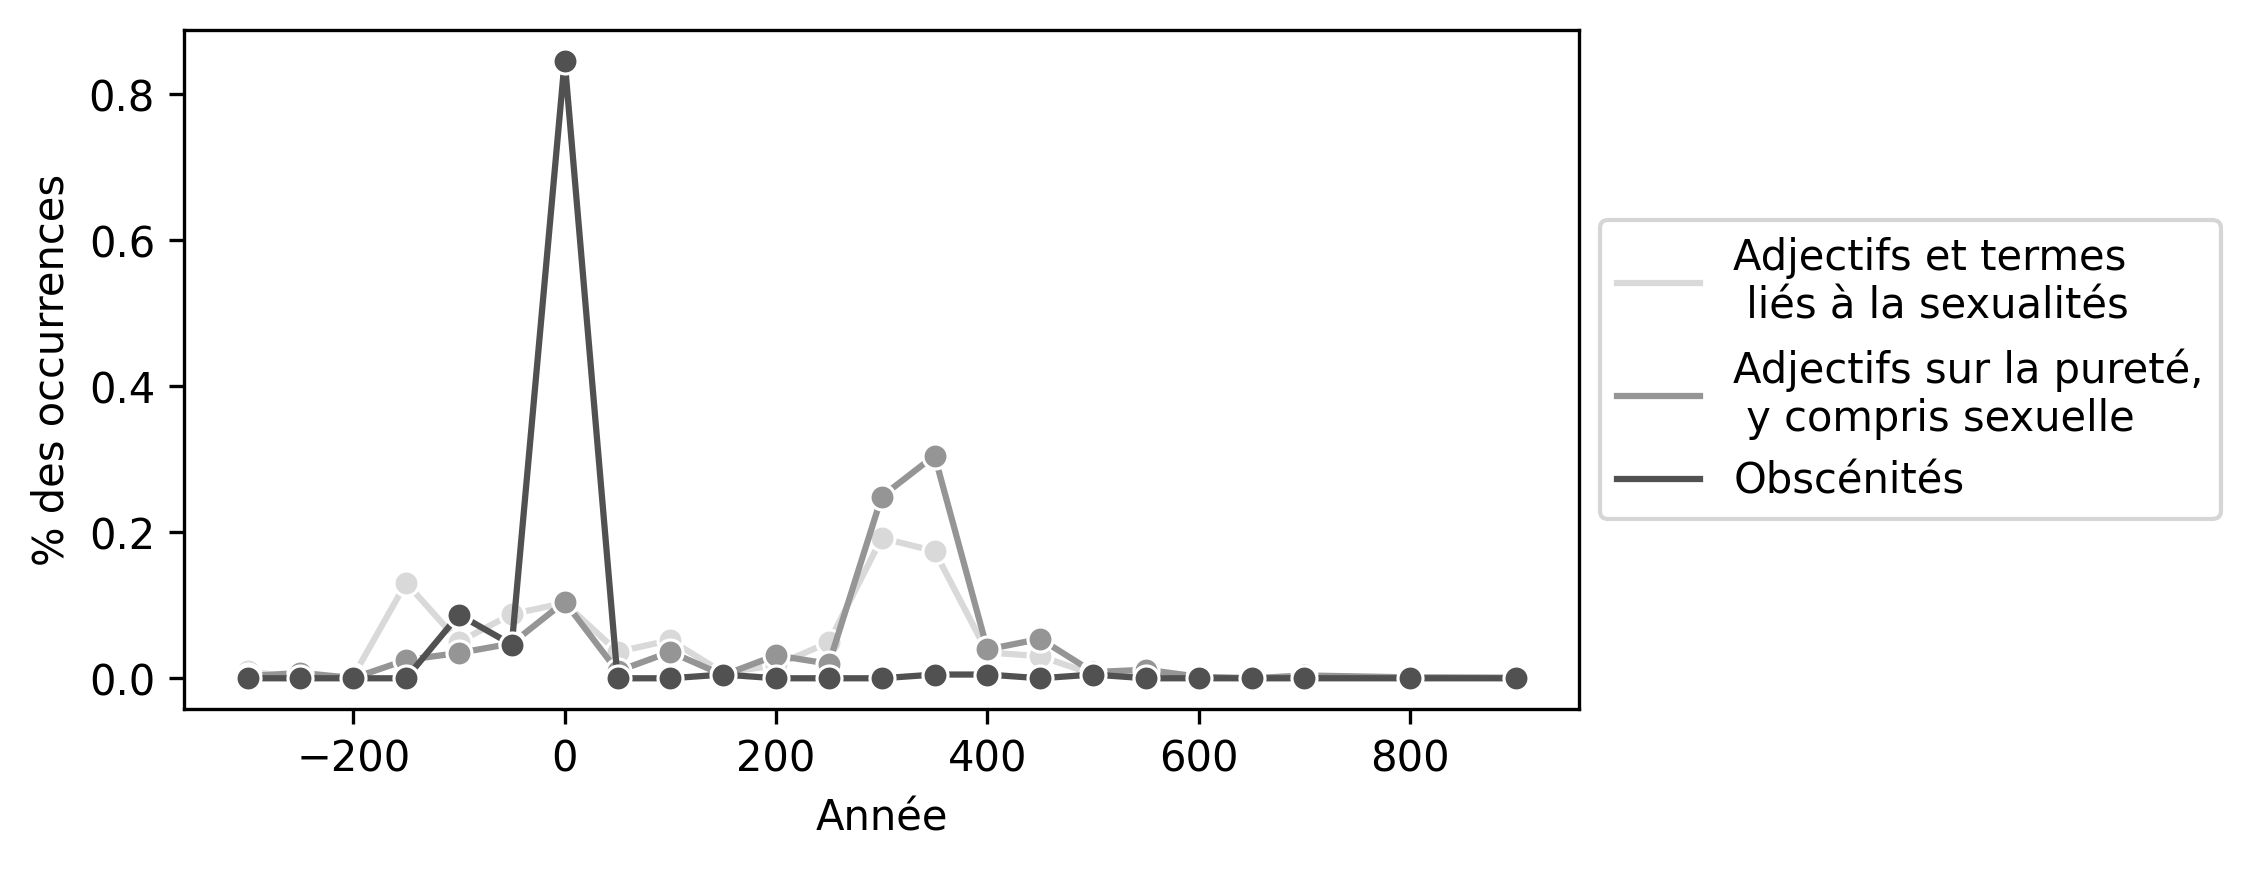
\includegraphics[width=\linewidth]{figures/chap1/part3/exemplier/exemplier_prcentage_occs.png}
    \caption{Part des occurrences de trois groupes lexicaux en fonction des années. Le groupe \textit{Obscénités} atteint 80\% de ses occurrences avec les auteurs nés entre 0 et 50.}
    \label{fig:exemplier:lexical_groups}
\end{figure}

Il ne faut pas non plus perdre de vue l'angle d'attaque d'Adams sur son livre pour expliquer cette chute. Si le IV\textsuperscript{e} siècle est beaucoup moins représenté, c'est aussi qu'il parle probablement de sexualité à travers d'autres termes, par exemple à travers des évaluations morales (\textit{lascivus}, \textit{impudicus}) ou par les louanges de l'absence de sexualité (\textit{virginitas}, \textit{puritas}). En guise d'aperçu, on analyse un regroupement autour de trois groupes lexicaux et la répartition de leurs occurrences sur le meta-corpus (\textit{cf.} figure \ref{fig:exemplier:lexical_groups}). Ces groupes lexicaux, imparfaits et ne cherchant qu'à évoquer un approfondissement nécessaire, sont:
\begin{enumerate}
    \item Les \enquote{adjectifs et termes liés à la sexualité}, soit la famille \textit{lasciv-}, \textit{mollis}, \textit{mollitia}, \textit{libido}, \textit{impurus}, \textit{voluptas}. 
    \item Les \enquote{adjectifs et termes liés à l'absence de sexualité}, en particulier la notion de virginité: \textit{virginitas}, \textit{purus}, \textit{puritas}.
    \item Les \enquote{obscénités} les plus marquantes et les plus fréquentes de la langue latine: \textit{mentula}, \textit{futuo}, \textit{pedico}, \textit{irrumo}, \textit{cunnus}.
\end{enumerate}

Il devient alors clair que les obscénités n'existent presque qu'à travers les auteurs nés entre -150 et 50, alors que les groupes (1) et (2) connaissent une explosion pendant la période chrétienne des premiers Pères de l'Église. Il ne peut s'agir ici que d'appuyer l'intuition d'un changement d'approche des discours sur la sexualité, qui n'a clairement pas été envisagée par Adams. Elle pose une question importante: la virginité fait-elle partie de l'espace sémantique de la sexualité ? Chez l'auteur du \textit{Latin Sexual Vocabulary}, il est clair qu'elle n'y fait partie que quand elle est enlevée: il n'y fait mention que dans ce contexte, qu'il s'agisse de \textit{uirginitatem eripio}\footcite[p.~195]{adams} (\enquote{arracher la virginité}), ou dans celui de métaphores permettant de parler du sexe féminin, telles que \textit{uirginalem scrobem}\footcite[p.~151]{adams} (\enquote{cavité virginale}) chez Arnobe.

Cette compilation et sa visualisation nous permettent ainsi de mettre encore une fois en lumière les forces et les faiblesses du travail d'Adams, comprenant un peu plus l'angle scientifique qu'il avait lors de la rédaction de son travail. Aline Rousselle dit dans son compte-rendu qu'Adams fait un \enquote{vocabulaire obscène et non, comme le dit le titre, [un] vocabulaire sexuel}\footcite{rousselle_j_1987}. Il nous semble du moins que l'auteur du \textit{Vocabulary} s'est attaché plus particulièrement à l'obscénité et à la sexualité \enquote{en cours} plutôt qu'à ce que nous qualifierions peut-être de \enquote{sexualité latente} ou de \enquote{discours sur la sexualité}, qu'il s'agisse de moralisation, où la sexualité n' est pas en action, mais est connexe au sujet, ou de description médicale.

\paragraph{Vers une interface de valorisation}

Ces données sont faites pour être utilisées: elles sont documentées par la présente recherche, s'accompagnent d'un schéma, et sont sous licence libre. Non seulement il n'est pas évident pour chacun de manipuler un document XML, mais en plus cette manipulation peut s'avérer lourde pour une consultation de quelques données croisées. Dans ce contexte, si nous avions tenté une approche par un export via LaTeX vers PDF -- sa maniabilité était équivalente à un papyrus calciné d'Herculanum à cause du nombre d'extraits qui composent l'exemplier -- c'est vers l'application web que nous nous sommes rapidement tourné.

Le squelette de l'application repose sur un cadriciel python pour le web, \textit{Flask}\footcite{ronacherpallets}, et un moteur de recherche en python pur, \textit{Whoosh}\footcite{whoosh}. Ce choix technique permet de réduire au maximum le code produit mais aussi de ne pas dépendre de services secondaires tels qu'\textit{Elastic Search}. L'application est nourrie par et exploite  les documents XML TEI qui sont simplement ingérées par le moteur à la construction de l'application. Tout le reste n'est qu'une simple mise en relation des facettes afin de pouvoir proposer des recherches multi-critères.

\begin{figure}
    \centering
    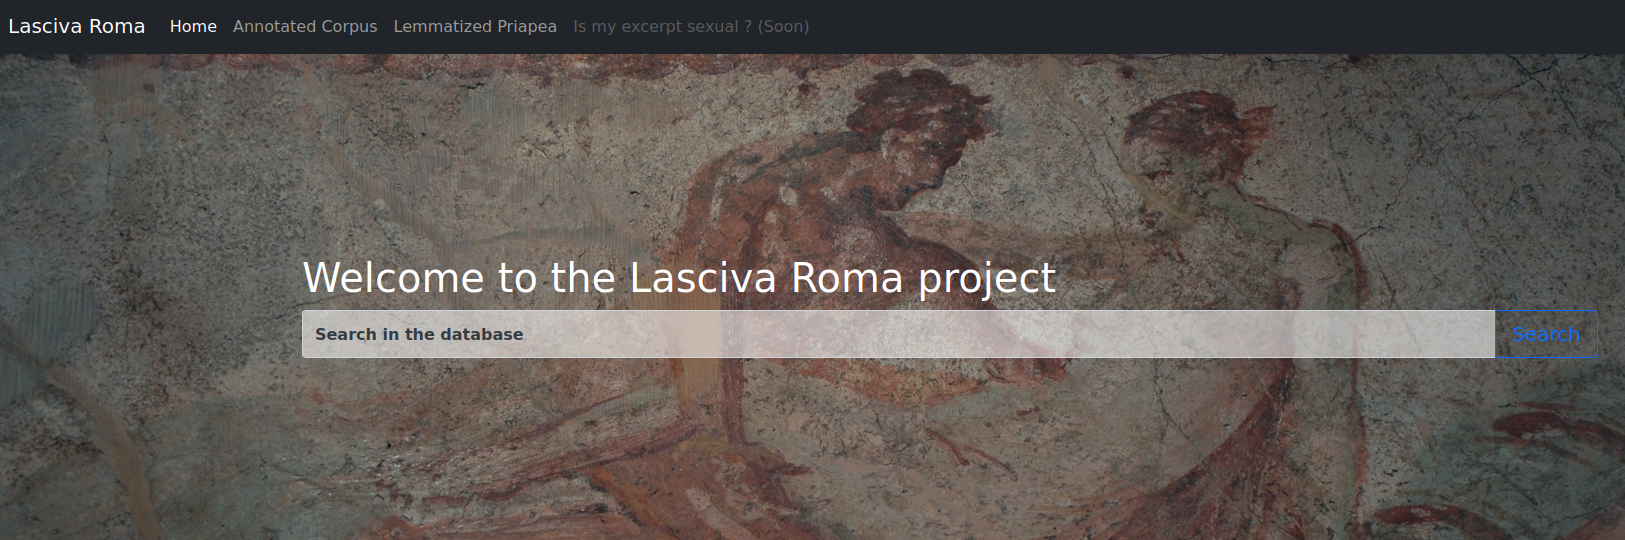
\includegraphics[width=.8\linewidth]{figures/chap1/part3/exemplier/AccueilInterface.png}
    \caption{Page d'accueil de \textit{Lasciva Roma}. L'objectif de l'application est d'accueillir l'ensemble des travaux issus de cette recherche.}
    \label{fig:exemplier:accueil}
\end{figure}

Cette application n'avait pas pour vocation l'exploitation des informations statistiques ni la visualisation de ces données. Cette forme de valorisation viendra dans l'application, même de manière réduite, pour mettre en valeur les requêtes effectuées par les utilisateurs et pour les contextualiser. Elle demande l'exploitation de statistiques issues du meta-corpus, qu'il faut alors compiler régulièrement. Par exemple, on pourrait avoir la fréquence relative d'un lemme dans l'exemplier numérique et sa fréquence relative dans le meta-corpus afin de montrer de potentielles sur-représentations.

\begin{figure}
    \centering
    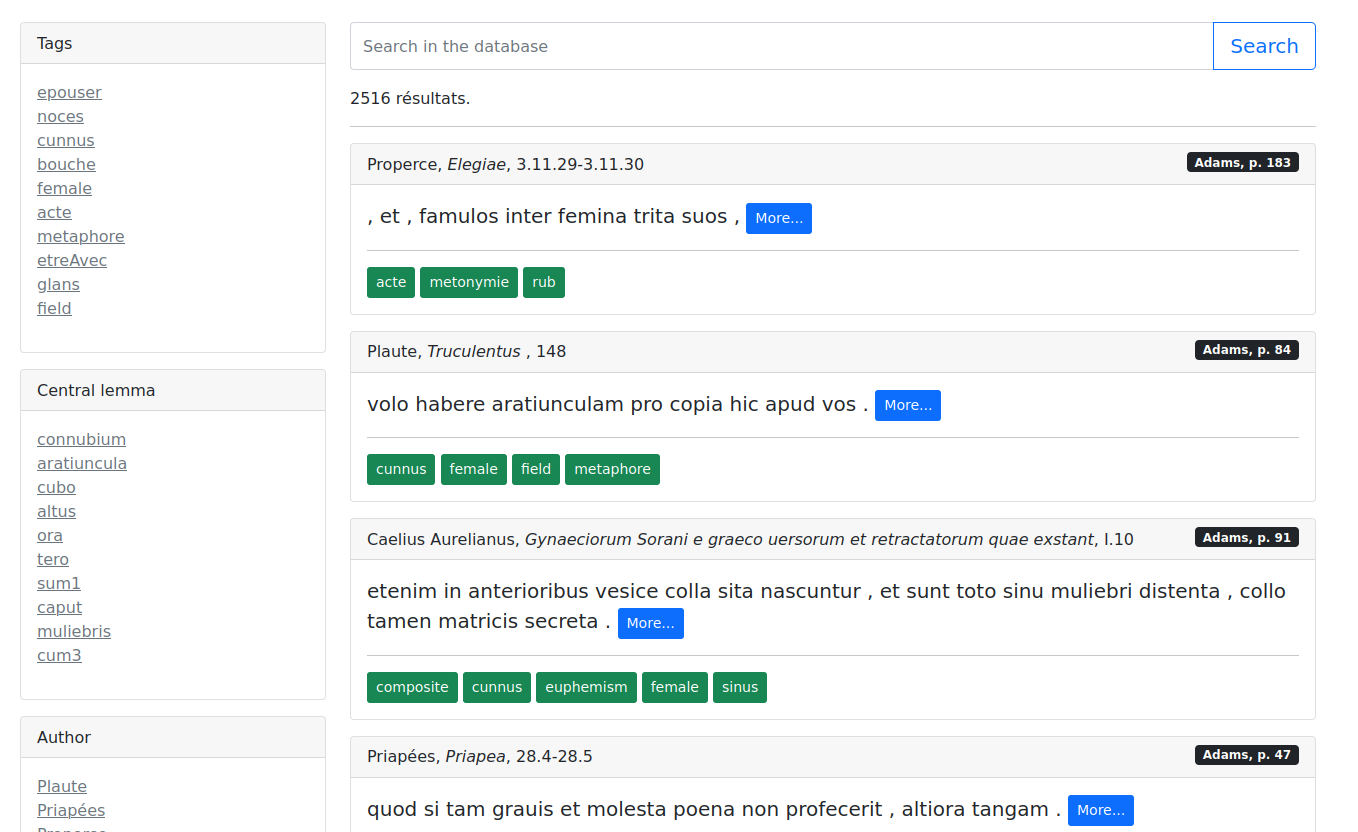
\includegraphics[width=.8\linewidth]{figures/chap1/part3/exemplier/IndexInterface.png}
    \caption{Page d'accueil de l'index.}
    \label{fig:exemplier:index}
\end{figure}

Cette application, nommée \textit{Lasciva Roma}, a pour but de faciliter la compréhension de certains extraits, familles de lemmes, catégories d'Adams en les mettant en regard. Elle permet, par exemple, de faire des recherche sur les formes, les lemmes, les lemmes annotés commentés par les sources secondaires, et les mots-clefs déployés dans celles-ci. Mais elle a aussi le même usage que l'exemplier papier, en offrant, à travers l'information de pagination, de circuler dans le corpus au fur et à mesure qu'Adams le déploie. Cette approche est enrichissante pour le lecteur d'Adams, car elle permet d'outrepasser le problème de place dans le livre imprimé qui a limité le lexicographe.

\begin{figure}
    \centering
    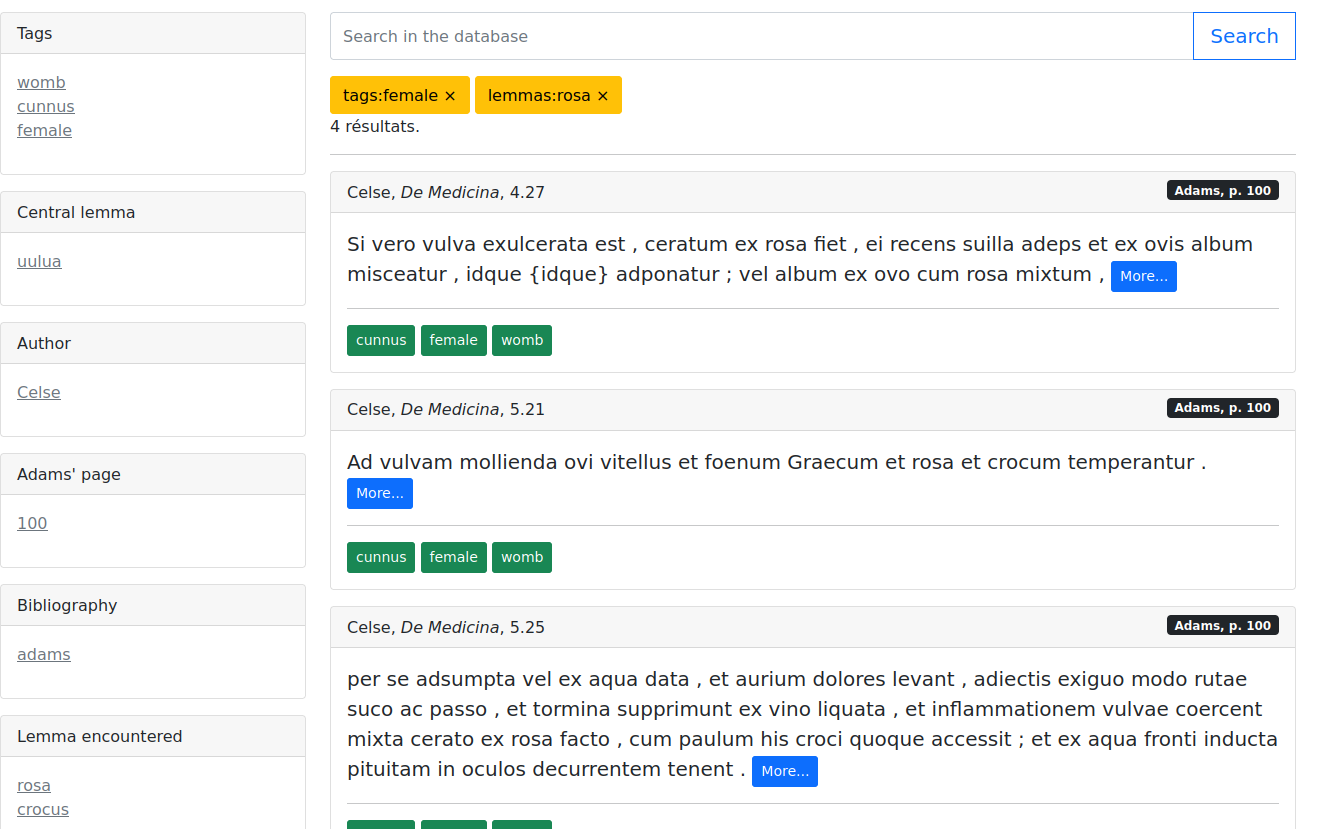
\includegraphics[width=.8\linewidth]{figures/chap1/part3/exemplier/RechercheFacette.png}
    \caption{Exemple de recherche à facette (combinaison de mots-clefs).}
    \label{fig:exemplier:recherche}
\end{figure}

Née d'un besoin précis, ponctuel et nourri de notre propre connaissance du corpus, l'application ne propose pas au moment de la restitution de nos travaux de fonctionnalités nécessaires à son utilisation par un public plus large. L'intégration d'index pour chacune des grandes portes d'entrée de l'exemplier (Bibliographie, Mot-Clef, Lemme commenté, Auteur, œuvre, Formes), et d'une fonctionnalité permettant de sélectionner un ensemble de pages chez Adams (par exemple, de la page 50 à 55) permettront d'enrichir encore plus la manipulabilité de l'application. À terme, l'intégration du thésaurus et de ses descriptions facilitera la compréhension de la base. La possibilité pour des contributeurs externes de recommander des sources secondaires ou des éléments de bibliographie de type (3), de proposer des \textit{mot-clefs} ou des traductions, amèneront la base à devenir ce qu'elle peut être: un incontournable exemplier numérique pour aborder la connaissance du \textit{vocabulaire} latin de la sexualité.

Sans enfermer les données dans une application, tout ouverte qu'elle soit, le développement de \textit{Lasciva Roma} permet d'aborder la place de l'applicatif dans la recherche scientifique. Cette application a pour vocation principale de mettre nos résultats à la disposition de l'ensemble de la communauté scientifique (et non uniquement la part réduite des humanités numériques), des enseignants du secondaire et des passionnés de la langue latine. À travers le schéma de ses données, la documentation de son infrastructure et la description de sa mise en place, elle peut aussi devenir une application adaptable à d'autres lexiques et favoriser la création de nouveaux exempliers numériques, à la fois ressources pédagogiques et de recherche.

% Représentation et sur-représentation des auteurs
%% Confirmer l’angle mort de l’étude d’Adams: la période Chrétienne sous-représentée ?
\clearpage
\section*{Conclusion: De la bande magnétique à l'exemplier numérique}

En un peu plus de cinquante ans, notre rapport aux textes antiques a été complètement bouleversé. La numérisation des corpus a d'abord changé notre manière de lire un texte: on passait alors d'un texte à un autre sans revenir aux étagères d'une bibliothèque, en tapant au clavier d'abord puis en cliquant. Puis, cette disponibilité du texte a dépassé les murs de la bibliothèque universitaire et du laboratoire: grâce à une simple connexion internet, on a eu alors facilement accès à de vastes corpus de textes sans même se déplacer.

En dehors même d'une question d'accès, le numérique a également favorisé un véritable changement épistémologique. Les textes antiques, en étant numérisés, se sont aussi défaits de leur linéarité, en devenant en partie des catalogues d'occurrences grâce auxquels le chercheur peut facilement rassembler des preuves, sans avoir à parcourir tous les rayons des bibliothèques  et toutes les pages de leurs ouvrages. Dans ce cadre, les récits d'expérience de John J. Hughes\footcite{helgerson_cd-rom_1988} ou de Peter Zahn\footcite[p. 427]{zahn_kirchenvater-texte_1992} sont exemplaires: le travail de compilation d'occurrences pour le premier, et une recherche d'attribution d'un inédit pour le second passent entre 1980 et 1992 de cinq jours de travail à moins de vingt-cinq minutes. 

Cette production de corpus a aussi eu le temps de devenir un domaine de la recherche, avec ses codes, ses interrogations et ses débats. La forme \enquote{d'incunable numérique} produite dans un \textit{far-west} technologique peinant à se stabiliser a laissé peu à peu sa place à des standards. La \textit{Text Encoding Initiative}, ses \textit{guidelines} et ses membres (fondateurs comme actuels) ont joué et jouent toujours un rôle prépondérant dans cette marche vers une production de corpus inter-opérables. Cela ne signifie pas que la discussion est close, tout comme celle concernant les pratiques de l'impression ne s'est pas terminée au XVII\textsuperscript{e} siècle. Cette question n'est d'autant pas fermée que la production d'éditions nativement numériques reste, comme nous l'avons vu, extrêmement rare dans le domaine latin: nous rattrapons pour l'instant à peine la couverture des corpus papiers, en en produisant des fac-similés numériques, souvent au détriment la richesse des apparats ou des commentaires.

Cette stabilisation permet non seulement la mise en place d'une linguistique de corpus mais aussi d'une \enquote{littérature de corpus} en appliquant de nouvelles méthodes à des questions anciennes et en faisant émerger de nouvelles interrogations. L'utilisation de corpus ne permettent plus simplement d'accélérer la recherche d'occurrences ou de passages, mais bien d'approcher les textes à travers les phénomènes statistiques qu'ils contiennent. C'est dans ce contexte que la production d'exempliers numériques peut aussi transformer les approches statistiques, En commençant à produire assez de données dans des domaines différents (guerre, couleurs, sexualité, etc.) peut permettre de tester, au sens informatique, des méthodes computationnelles et de les évaluer quantitativement et qualitativement. Ces évaluations permettraient alors de valider d'autant plus de nouvelles méthodes, qui elles-mêmes révèleront de nouvelles facettes du domaine latin.

À la croisée de la mise à disposition des données et de leur exploitation, les corpus et exempliers numériques ont transformé et transforment notre approche de la langue et de la culture latine. En sortant le texte du format papier et en le mettant en réseau, nous nous sommes défaits de \enquote{l'obligation} de lire le texte de manière linéaire. À partir du moment où ces textes et corpus se sont retrouvés sont devenus librement accessibles, non pas comme des textes sur interface, mais comme des données manipulables et ouvertes, nous nous sommes donnés les capacités de produire une nouvelle méthode des sciences de l'antiquité, de la philologie ou des sciences humaines en général.

% Il ne s'agit plus alors que de simplement chercher un passage ou des occurrences d'un lemme pour rendre le travail plus rapide du chercheur,

% Changements épistémologiques et apports du numérique \enquote{libre}
   %  Le saut épistémologique introduit par les corpus électroniques
   %  Repenser la catégorie de corpus
  
\chapter{Principes généraux du \textit{deep learning} liés au TAL}

Les statistiques ont intéressé relativement tôt plusieurs branches des sciences humaines, dont celles du domaine classique avec l'histoire quantitative ou la linguistique de corpus. Les statistiques ont alors un rôle relativement simple: permettre d'observer des phénomènes à distance du texte ou des données récoltées par l'histoire, et établir ainsi des règles par exemple. Depuis maintenant plusieurs décennies, on s'est aussi rendu compte dans ces mêmes domaines que les mathématiques et l'informatique offraient d'autres possibilités, en particulier ce que l'on appelle l'\textit{apprentissage machine} (\textit{machine learning}): il devient possible d'enseigner à un programme à analyser des phénomènes, par exemple syntaxiques ou sémantiques. Pour faire cela, les programmes se composent d'ensemble de formules mathématiques comprenant des variables qui, en voyant des données, vont s'adapter à ces dernières pour reconnaître comme l'être humain des motifs permettant de les classer. Si l'on apprenait à la machine à reconnaître des noms propres, le premier indice serait souvent une majuscule à l'initiale: c'est un premier motif validant l'hypothèse.

L'apprentissage machine commence par l'entraînement: il faut donner à la machine des données, lui dire quelle est la réponse attendue. C'est le même phénomène avec les enfants en bas âge et l'acquisition du langage: à force de répéter que tel objet est une voiture, l'enfant intègre "Machine à 4 Roues" = Voiture. La machine va pendant cet entraînement modifier les variables qui constituent son modèle mathématique: en somme, c'est toujours la même formule qui est appliquée, mais la machine va décider au fur et à mesure de l'importance de chacune des informations. Par exemple, pour les noms propres, elle comprendra peu à peu que l'information position dans la phrase et majuscule à l'initiale sont très importantes, tandis que les suffixes ne le sont pas forcément... Ces valeurs de variables de l'algorithme sont appelées \textit{poids} ou \textit{paramètres} et constituent une retranscription mathématique de ce que la machine a appris. 

\begin{figure}[h]
    \centering
    \begin{equation*}
        \begin{matrix}
            \textrm{\textit{Mot}} \\
            \begin{bmatrix}
            \textrm{Commence par une majuscule} \\
            \textrm{Premier mot dans la phrase} \\
            \textrm{Précédé d'une préposition} \\
            \textrm{...} \\
            \end{bmatrix}
        \end{matrix}
        \rightarrow
        \begin{matrix}
            \textrm{Fortissimi sunt Belgae} \\
            \begin{bmatrix}
            1 & 0 & 1 \\
            1 & 0 & 0 \\
            0 & 0 & 0 \\
            & \textrm{...} & \\
            \end{bmatrix}
        \end{matrix}
        \rightarrow Algorithme \rightarrow
        \begin{matrix}
            \textrm{Résultat} \\
            \begin{bmatrix}
            0 & 0 & 1 \\
            \end{bmatrix}
        \end{matrix}
        \end{equation*}
    \caption{Exemple de représentation de la phrase "Fortissimi sunt Belgae.". Les trois colonnes représentent les données, les lignes représentent des variables (on parle aussi de \textit{features}). Le résultat est une matrice à une seule dimension (un vecteur) comprenant 1 pour les noms propres, et 0 pour les autres.}
    \label{fig:deep-learning:matrice}
\end{figure}

Pour représenter les données, et pour effectuer des calculs dessus, l'apprentissage machine se base sur l'algèbre linéaire: il s'agit d'une partie des mathématiques considérant les nombres sous la forme de matrices et de vecteurs. Les matrices correspondent plus ou moins à des tableaux de données: elles sont réparties sur plusieurs dimensions, la plus facile à représenter pour nous étant les matrices à deux dimensions (\textit{cf.} Table \ref{fig:deep-learning:matrice}). En effet, un tableau, avec x colonnes et y lignes est tout simplement une matrice à 2 dimensions (x, y). Les colonnes et les lignes forment alors des associations qui mathématiquement permettent de mettre en exergue des informations supplémentaires.

En traitement automatique des langues, on a recourt à l'apprentissage machine pour deux grands types de tâches:
\begin{itemize}
    \item \textbf{La classification} de valeurs. Il peut s'agir de chercher à annoter des mots comme noms propres, comme adjectifs, comme sujet, etc. ou encore de classer des phrases par thèmes ou des textes par auteurs.
    \item \textbf{La génération} de texte. Elle est désormais commune dans la traduction automatique, mais aussi dans la création de robot de discussion pour les plateformes en ligne. On distinguera les générations caractère par caractère des générations mot par mot, chacune possédant des facultés différentes: la possibilité pour l'une de trouver de nouvelles formes morphologiques, pour l'autre, l'impossibilité de proposer un mot inexistant.
\end{itemize}{}

En pleine croissance depuis une dizaine d'années, l'apprentissage profond se distingue dans l'apprentissage machine principalement sur deux points: d'une part, l'absence de nécessité pour le développement d'un modèle de faire le tri manuellement parmi les données à prendre en compte (on parle d'absence de \textit{feature extraction}); d'autre part, parce que la machine ingère plus de données, elle a besoin d'une architecture mathématique plus complexe et donc de beaucoup plus de puissance de calcul. Certaines tâches, comme l'attribution d'auteur, existent à la fois comme tâche classique et comme tâche d'apprentissage profond. En apprentissage machine "classique", on sélectionne entre autres les mots les plus fréquents de la langue, les mots outils (déterminants, verbes d'état, conjonctions de coordination, etc.) et on récupère leur fréquence dans chaque texte à classer\footnote{Il existe bien d'autres paramètres utilisables, \textit{cf.} \cite{Cafieroeaax5489}}. Dans le domaine latin, en poésie latine pour être précis, les formations rythmiques\footcite{nagy_metre_nodate} ont pu être utilisées comme variables d'entrée et produire des résultats très pertinents. Au contraire, en apprentissage profond, on aura tendance à fournir le texte de manière brute ou un minimum prétraité (selon que l'on s'intéresse aux caractères plutôt qu'aux mots). C'est par exemple le procédé proposé par Ruder et al. \footcite{ruder_character-level_2016} dans une étude sur l'attribution d'auteurs sur Twitter: pour gérer des textes courts, avec des orthographes variées, leur proposition fut de prendre le texte brut et de traiter les caractères en brut comme données d'entraînement. Il reste au programme à faire le travail, par conjectures, d'identification des motifs importants.

On distingue parmi ces catégories de l'apprentissage machine deux approches exclusives: les méthodes non supervisée et supervisée. Tout comme l'humain, ces programmes sont capables de rapprocher des éléments ensemble: si un objet possède quatre roues, des portes, il est probable qu'il s'agisse de la même chose, les camions et les voitures possèdent donc une proximité, il n'est pas nécessaire de dire qu'il s'agit de véhicules. Mais elle peut aussi apprendre par injonction et correction: une automobile et un carrosse ont 4 roues, mais on enseigne à la machine qu'ils représentent deux catégories distinctes d'objet. La différence fondamentale entre les deux protocoles réside dans la présence dans les données fournies à l'entraînement des résultats attendus. Fondée sur leur absence, la méthode non supervisée va effectuer des rapprochements entre les données par assimilation: en traduction automatique, du français vers l'anglais par exemple, la machine repèrera facilement que la présence de \textit{est} se traduira par une présence de \textit{is}. En traitement automatique du langage et en apprentissage profond, cette méthode est principalement utilisée, outre le cas précédent, pour créer des corpus: on le retrouve par exemple sur des agrégateurs tels que \textit{Google News} où les articles sont rassemblés par thème en fonction de la proximité de leur sujet. Il n'y a pas - ou peu - d'éditorialisation humaine dans ce genre de procédé. Au contraire, en supervisé, on donnera à la machine à reconnaître Molière de Corneille en lui disant: ce texte est de Corneille, ce texte est de Molière, etc. 

Pour être précis, pour cette dernière méthode, la machine joue en quelque sorte à un jeu de chaud et froid avec les données: à chaque fois qu'elle donne une réponse, elle est comparée à la réponse attendue. L'écart entre ces réponses est une mesure mathématique appelée \textit{loss} (perte). Cette perte est d'ailleurs transmise à l'algorithme pour affiner ses poids, et le programme a alors pour objectif de réduire cet écart le plus possible: on appelle cela la \textit{rétropropagation} (\textit{backpropagation}). Un entraînement va voir ces données plusieurs fois, jusqu'à atteindre une impossibilité d'apprendre plus: on appelle ces cycles de consultation des \textit{epochs} (époques). Comme avec un enfant en bas âge, la répétition permet à la machine d'assimiler les motifs et de proposer les réponses attendues en s'y adaptant mathématiquement. Une fois le modèle entraîné, il peut être utilisé sur des données sans réponse connue: on parle alors d'inférence ou de prédiction, et le modèle n'apprend plus.

\begin{table}[h]
\centering
\begin{tabular}{lllccc}
\toprule
\multirow{2}{*}{Texte} & \multirow{2}{*}{Étiquette réelle}& \multirow{2}{*}{Étiquette de prédiction} & \multicolumn{3}{l}{Catégorie de classification} \\
                       &                         &                             & Corneille        & Molière       & Racine       \\ \midrule
Le Cid                 & Corneille               & Corneille                   & VP               & VN            & VN           \\
Le Misanthrope         & Molière                 & Molière                     & VN               & VP            & VN           \\
Phèdre                 & Racine                  & Racine                      & VN               & VN            & VP           \\
L'Avare                & Molière                 & Racine                      & VN               & FN            & FP          \\ \bottomrule
\end{tabular}
\caption{Exemple de classification avec les catégories afférentes. VP = Vrai Positif, FP = Faux Positif, VN = Vrai Négatif, FN = Faux Négatif}
\label{deep-learning:table:true-positives}
\end{table}

Pour mesurer l'efficacité d'un modèle supervisé, on le teste. Pour cela, on coupe généralement un corpus de données entre des données d'entraînement (\textit{train data}) et de test (\textit{test data}). On compare ensuite chacune des prédictions du modèle obtenu avec les étiquettes données dans le corpus, que l'on appelle vérité de terrain (\textit{ground truth}). Les étiquettes sont regroupées en classes: par exemple, dans le cas de Molière et Corneille, nous avons deux classes, et si nous avons 128 textes, nous avons 128 étiquettes réparties entre ces deux classes. Les résultats sont regroupés ensuite dans 4 catégories (\textit{cf.} \ref{deep-learning:table:true-positives}): les vrais positifs (VP/TP, bonne étiquette), faux positifs (FP, mauvaise étiquette pour la classe actuelle), vrais négatifs (VN/TN, reconnu comme n'étant pas de cette étiquette), faux négatif (FN, étiquette de la classe actuelle non reconnue); si toutes les étiquettes sont dans les catégories qualifiées de vraies, le modèle n'a fait aucune erreur. Ces écarts à la vérité sont mesurés principalement par 4 formules qui fournissent des pourcentages (100\% étant le meilleur score):
\begin{itemize}
    \item L'\textit{accuracy}\footnote{Le choix a été fait de ne jamais traduire \textit{accuracy} en raison de sa traduction en "précision" qui crée la confusion avec l'autre mesure \textit{precision}} mesure le nombre de vrais positifs sur le nombre total d'éléments annotés, et on pourrait le ramener à un pourcentage classique de bonne réponse. En machine learning, on le définit aussi par la formule correspondante $accuracy = \frac{VP + VN}{VP + VN + FP + FN}$
    \item La \textit{precision} mesure le pourcentage de bonnes réponses par classe sur l'ensemble des attributions effectuées sur cette classe. Elle favorise les attributions correctes à une classe sans prendre en compte les non-attributions. Sa formule est $precision = \frac{VP}{VP + FP}$
    \item Le \textit{recall} (rappel) mesure le pourcentage de réponses correctes sur l'ensemble de la classe. Elle favorise la reconnaissance de chacune des classes plutôt que les mauvaises attributions. Sa formule est $recall = \frac{VP}{VP+FN}$.
    \item Le F-Score (qui peut se découper en F1-, F2-, etc.) est la moyenne harmonique de la précision et du rappel, offrant ainsi une mesure intermédiaire. Sa formule est $F1 = \frac{2 \cdot precision\cdot recall}{precision+ recall}$
\end{itemize}{}

\label{deep-learning:overfitting}
Un risque de l'entraînement est de se retrouver avec un modèle qui apprend les réponses par coeur pour chaque donnée d'entrée: à ce moment-là, il sera incapable de gérer des données extérieures. Une des sources du problème peut être un corpus d'entraînement trop homogène: la catégorie nom propre ne comprend que des phrases où les noms propres sont précédés d'une abréviation (M., Mme, etc.), la machine apprend qu'un nom propre nécessite leur présence. On appelle cela un phénomène de \textit{surspécialisation} (\textit{overfitting}) au corpus d'entraînement\footnote{Par ailleurs, le phénomène étant clairement dû au corpus dans cet exemple, on parle aussi de biais de corpus.}. Sans que cela soit toujours le cas, une \textit{accuracy} à 100\% sur un corpus d'entraînement ou une loss de 0 est souvent l'un de ces signes. Pour éviter cela, on peut faire appel à plusieurs stratégies, non exclusives:
\begin{itemize}
    \item l'utilisation d'un corpus de développement ou d'évaluation (\textit{dev/eval corpus}). Il est vu lors de l'entraînement, mais n'est pas utilisé pour l'apprentissage: les erreurs ne sont pas individuellement transmises à l'algorithme. Cependant, sa perte, ou toute mesure sélectionnée dans ce cadre sont utilisées comme grand indicateur de fonctionnement: si le corpus d'entraînement fait 100\%, mais que le corpus de développement fait 80\%, on indiquera au modèle qu'il faut continuer à apprendre, quitte à s'éloigner des 100\%.
    \item l'utilisation, dans l'architecture du modèle, de \textit{dropout}, c'est-à-dire la suppression aléatoire d'une partie des données d'entraînement à chaque époque. En traitement automatique de la langue, il s'agit principalement de supprimer un mot par exemple.
\end{itemize}


\begin{figure}[h]
    \centering
    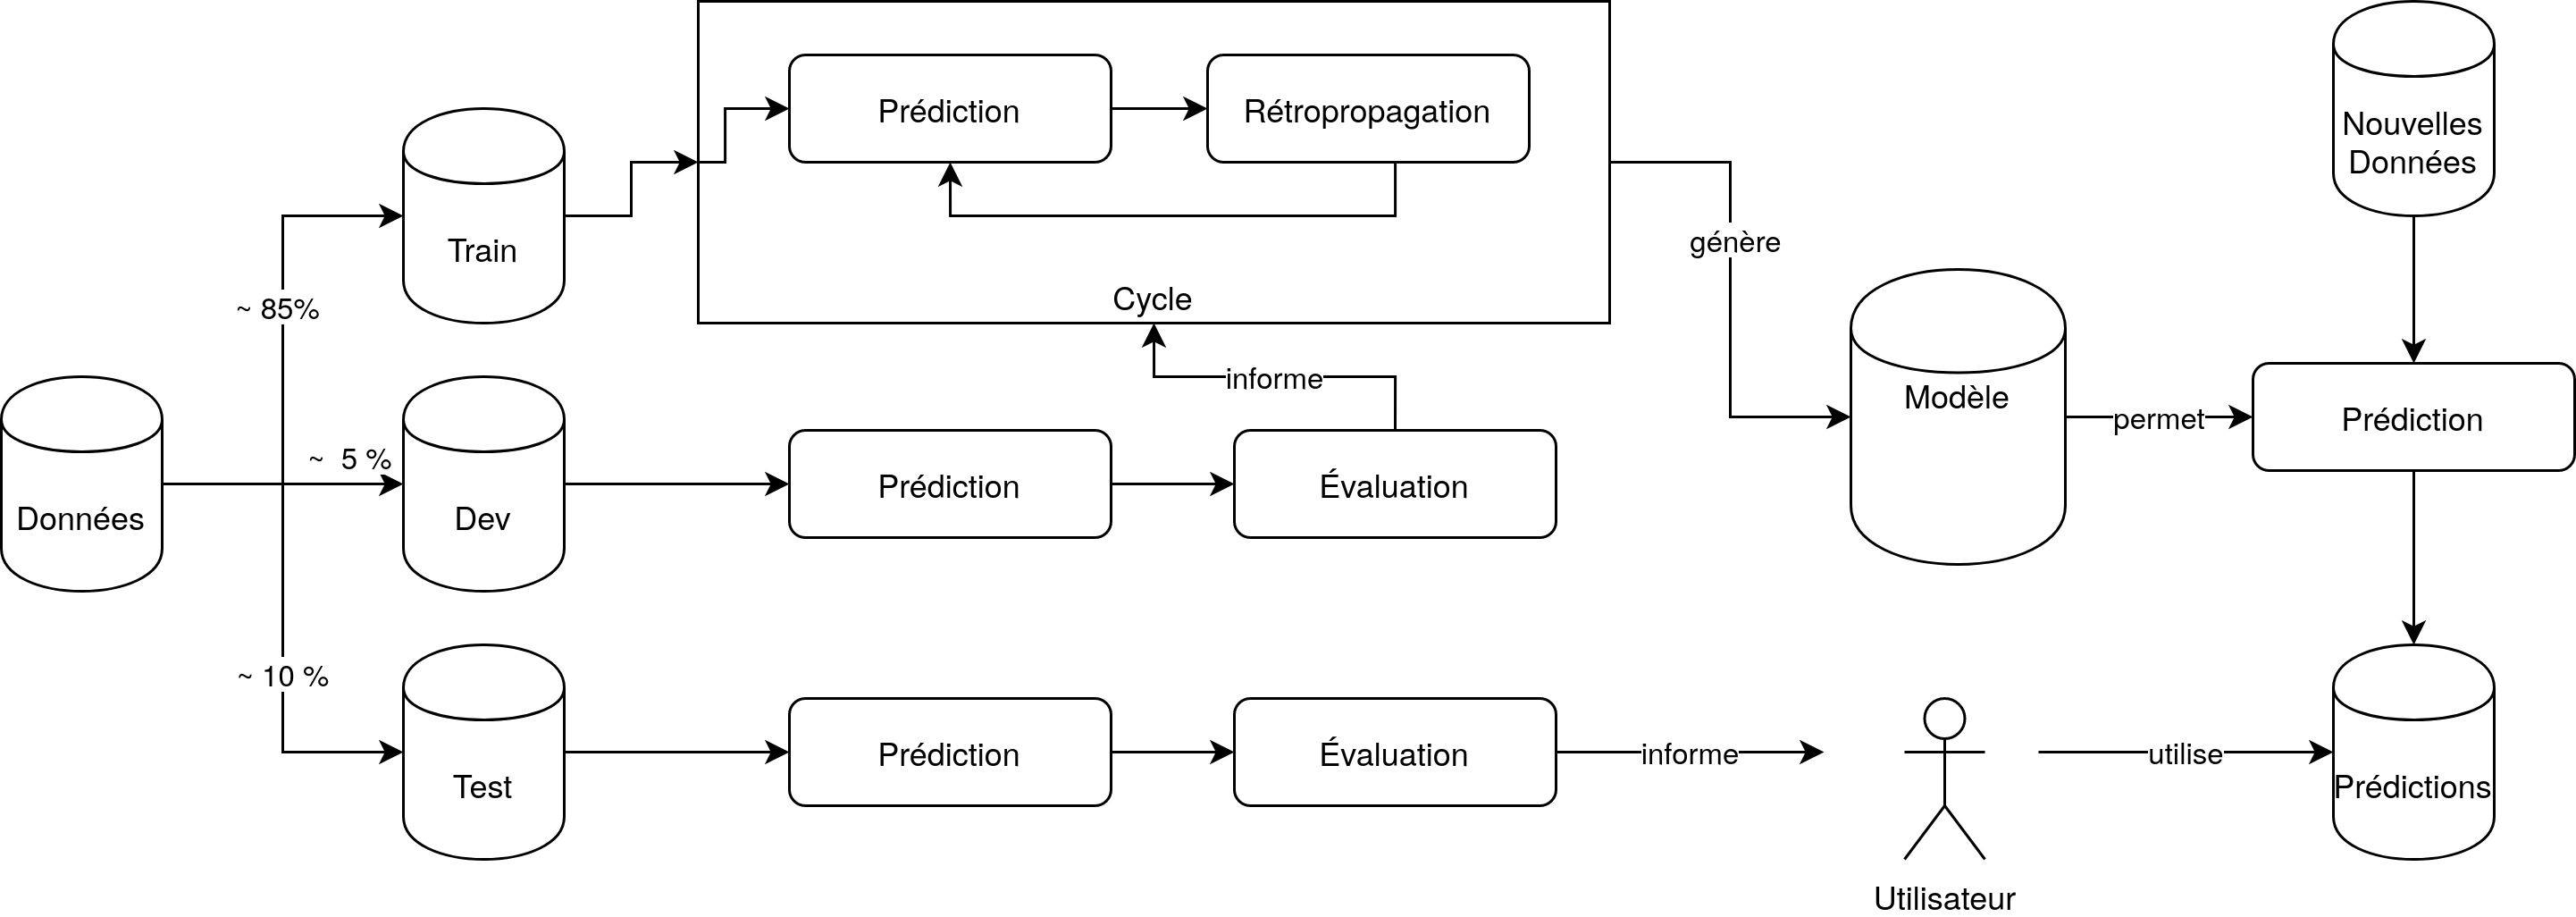
\includegraphics[width=\linewidth]{figures/chap2/MachineLearning.png}
    \caption{Étapes, rôles et fonctionnement de l'apprentissage machine supervisé.}
    \label{fig:deep-learning:fonctionnement}
\end{figure}

Enfin, on parle ici et là d'hyperparamètres d'architecture: il s'agit principalement de variables de configuration qui, pour un modèle, changent l'architecture ou sa manière de s'entraîner. L'un d'eux, très commun, est nommé \textit{learning rate}: il s'agit d'un nombre (principalement un décimal, de type 0.001) qui sert de pas pour corriger les erreurs du modèle. Plus il est bas, plus le modèle met de temps à apprendre; plus il est haut, plus le modèle risque de rater la bonne direction d'apprentissage. D'autres hyperparamètres concernent généralement la taille des réseaux neuronaux qui composent l'architecture. 

On retrouve en traitement automatique des langues quelques modules d'architecture très communs que l'on se propose d'expliquer, en partie, ici. Ces modules sont très souvent combinés ensemble: il est rare de voir une architecture complètement basée sur un seul de ces éléments.

\section{Embeddings}
\label{deep-learning:embeddings}

Une première difficulté pour la machine est de comprendre ce qu'est un mot. Puisque la machine, pour son calcul, doit opérer par nombres, la première option est donc de dire: à chaque mot, un chiffre. Si l'on a deux phrases, par exemple "\textit{fortissimi sunt belgae}" et "\textit{timendi sunt belgae}", à chaque mot nouveau un chiffre serait attribué, et l'on donnerait à l'algorithme les nombres 1, 2 et 3 puis 4, 2, 3: 2 et 3 sont présents deux fois, on ne réattribue pas d'identifiant numérique à \textit{sunt} et \textit{belgae}, par contre, \textit{timendi} qui est nouveau poussera à la création d'un nouvel identifiant, 4. On appelle ces nombres valeurs symboliques, et le résultat final \textit{one-hot vector}. Enfin, l'index des mots est considéré comme une variable discrète: son nombre de possibilités est fini (on peut les énumérer)\footnote{Une variable discrète est une variable dont on peut énumérer les valeurs (1, 2, 3, 4, etc.). par opposition à une variable continue (0.000000001, 0.000000002, etc.)}. Malheureusement pour la machine, ce caractère discret de la variable rend très difficile de faire un rapprochement entre 4 (timendi) et 1 (fortissimi): ils n'ont mathématiquement rien à voir ensemble. 

Dans notre langage, nous utilisons en fait déjà une forme de mathématisation des sens. Les expressions du type "\textit{timendi} est proche de \textit{fortissimi}" sont des métaphores de spatialisation: si l'on devait dessiner une carte des mots des deux phrases de l'encodage précédent, notre approche serait sûrement de rapprocher les deux précédents tandis que \textit{sunt} et \textit{Belgae} seraient autre part sur la carte. Faire cela, c'est projeter sur deux dimensions d'un plan (x et y) les sens des mots. On peut pousser cela en 3 dimensions, 4 dimensions, etc. Si chacune de ces colonnes était une catégorie de sens, on pourrait alors affiner et représenter chacun de ces mots (\textit{cf.} Figure \ref{figure:deep-learning:projection-embedding}). Bien sûr, ces colonnes ne sont pas aussi simplement lisibles, mais font suffisamment sens pour que la machine en fasse usage: cette représentation que la machine construit est issue d'un module de réseau que l'on appelle \textit{embeddings}\footnote{Par habitude, on appelle aussi le produit du réseau \textit{embeddings}.}. 

Au fur et à mesure de l'apprentissage, la machine fige alors une représentation de chacun des mots qui sera utile au reste du réseau (\textit{cf.} figure \ref{figure:deep-learning:embeddings-encoding}). Dans l'exemple précédent, on établit une matrice de $N$ par $M$, où $N$ correspond au nombre de mots différents rencontrés (ici 4) et $M$ une dimension de projection choisie (ici 2). La matrice d'embeddings, si l'on avait par exemple un apprentissage en vue d'une classification par sens ou d'une classification par nature de mot, aura tendance à proposer des résultats tels que dans la figure précédente, avec un rapprochement évident pour l'être humain, mais aussi désormais pour la machine de \textit{timendi} et \textit{fortissimi}. La machine apprend alors à reconnaître des éléments par leur contexte: pour des mots, ce principe repose sur le principe de distributionnalité\footcite{firth_papers_1957} qui veut que deux mots se ressemblant (sémantiquement, syntaxiquement, etc.) aient le même contexte\footnote{Nous proposons une étude de ce qu'apprend l'algorithme en fonction de la tâche en \ref{subsec:lemma_resultats}.}.

% Exemple d'encodage one hot

\begin{figure}
    \centering
    \noindent\begin{minipage}{.32\linewidth}
        \begin{equation*}
            \begin{bmatrix}
            fortissimi \\ 
            sunt \\ 
            Belgae \\ 
            timendi \\ 
            ... \\ 
            ... \\ 
            ... \\ 
            \end{bmatrix}
            \rightarrow \begin{bmatrix}
            1 \\ 
            2 \\ 
            3 \\ 
            4 \\ 
            ... \\ 
            ... \\ 
            n \\ 
            \end{bmatrix}
        \end{equation*}
    \end{minipage}%
    \begin{minipage}{.32\linewidth}
        \begin{equation*}
            \begin{matrix}
            \textrm{Fortissimi sunt Belgae}\\ 
            \textrm{Timendi sunt Belgae}
            \end{matrix}
            \rightarrow
            \begin{matrix}
            \left [ 1\;  2\;  3 \right ]\\ 
            \left [ 4\;  2\;  3 \right ]
            \end{matrix}
        \end{equation*}
    \end{minipage}
    \caption{Exemple d'encodage\textit{ one-hot}. On constitue d'abord un dictionnaire de transcodage, puis on traduit à l'aide de celui-ci les phrases}
    \label{deep-learning:one-hot-encoding}
\end{figure}

\begin{figure}[h]
    \centering
    \noindent\begin{minipage}{.45\linewidth}
        \resizebox{\linewidth}{!}{%
            \begin{tabular}{l|lll}
             & Féminin & Jeunesse & Royal \\ \midrule
            Homme                          & 0       & 0        & 0     \\
            Femme                          & 1       & 0        & 0     \\
            Garçon                         & 0       & 1        & 0     \\
            Fille                          & 1       & 1        & 0     \\
            Prince                         & 0       & 1        & 1     \\
            Princesse                      & 1       & 1        & 1     \\
            Reine                          & 1       & 0        & 1     \\
            Roi                            & 0       & 0        & 1     \\
            Monarque                       & 0.5     & 0.5      & 1    
            \end{tabular}%
        }
    \end{minipage}
    \begin{minipage}{.45\linewidth}
        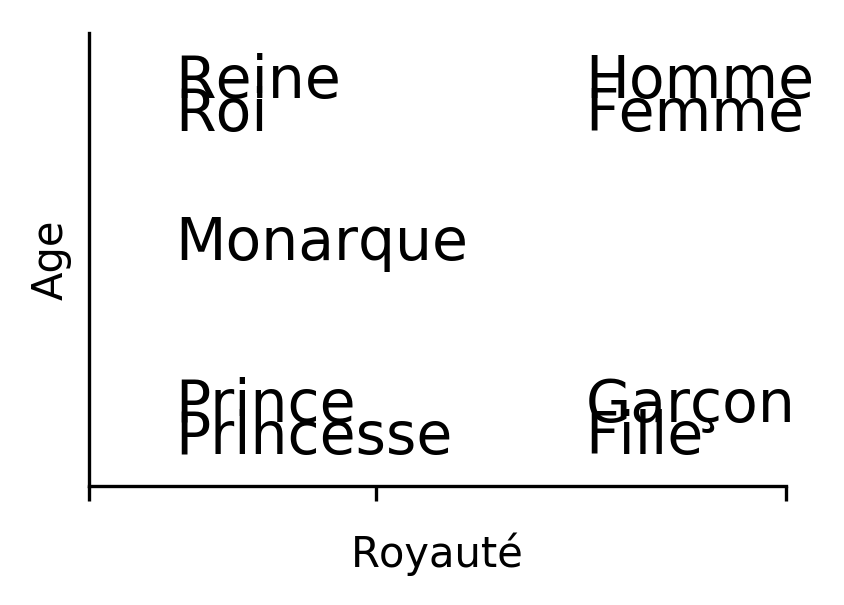
\includegraphics[width=\linewidth]{figures/chap2/visualisation_embedding.png}
    \end{minipage}
    \caption{En choisissant des catégories adaptées, il est possible de placer dans un tableau tout un ensemble d'informations et de différencier des éléments de vocabulaire mathématiquement. Ici, \textit{monarque} est neutre, il n'est donc ni féminin (1) ni masculin (0). Une fois ces catégories choisies, on peut les représenter sur deux dimensions via PCA. On remarque alors que les groupes se rassemblent. Inspiration: Lynn, Shane\footcite{lynn_get_2018}}
    \label{figure:deep-learning:projection-embedding}
\end{figure}

\begin{figure}[h]
    \centering
    \noindent\begin{minipage}{.32\linewidth}
        \begin{equation*}
            \begin{matrix}
            Fortissimi \\ 
            sunt \\ 
            Belgae \\ 
            timendi \\ 
            ... \\ 
            ... \\ 
            ... \\ 
            \end{matrix}
            \rightarrow 
            \begin{bmatrix}
            0.97 & 0.85 \\ 
            0.12 & 0.85 \\ 
            0.54 & 0.28 \\ 
            0.92 & 0.90 \\ 
            ... & ... \\ 
            ... & ... \\ 
            n & ... \\ 
            \end{bmatrix}
        \end{equation*}
    \end{minipage}%
    \begin{minipage}{.32\linewidth}
        \begin{equation*}
            \begin{matrix}
                \textrm{Fortissimi sunt} \\ 
                \textrm{Belgae} \\ \\
                \textrm{Timendi sunt} \\
                \textrm{Belgae}
            \end{matrix}
            \rightarrow
            \begin{matrix}
            
            \begin{bmatrix}
            0.97 & 0.85 \\ 
            0.12 & 0.85 \\ 
            0.54 & 0.28 \\ 
            \end{bmatrix} \\ \\
            
            \begin{bmatrix}
            0.92 & 0.90 \\
            0.12 & 0.85 \\ 
            0.54 & 0.28 \\ 
            \end{bmatrix}
            
            \end{matrix}
        \end{equation*}
    \end{minipage}
    \caption{Remplacement de l'encodage one-hot par une couche  embedding. La proximité entre les vecteurs de \textit{Fortissimi} et \textit{Timendi} et la répétition des deux autres mots produisent deux phrases très proches mathématiquement.}
    \label{figure:deep-learning:embeddings-encoding}
\end{figure}

Bien sûr, les dimensions des embeddings sont ordinairement beaucoup plus grandes que dans l'exemple construit ici: David Bamman, lors de la création d'une telle matrice sur l'ensemble des mots présents dans les livres classés langue latine du site archives.org\footcite{bamman_11k_2012}, a créé une matrice de $N=2,961,867$ et de $M=100$ (100 est une dimension assez habituelle pour $M$). 

\section{Réseaux Linéaires}
\label{deep-learning:linear}

Si les \textit{embeddings} permettent de générer une représentation des données, les modèles \textit{linéaires}\footnote{On le retrouve sous plusieurs noms: \textit{perceptron}, \textit{linear network}, \textit{dense layer}, \textit{régression linéaire}, etc.} permettent de les classer. Ce modèle est l'élément le plus simple d'un réseau neuronal (\textit{cf.} figure \ref{fig:deep-learning:simple-linear}). Par ailleurs, une couche linéaire peut être accumulée à d'autres couches linéaires, souvent en réduisant peu à peu la taille du réseau jusqu'à arriver à la taille de sortie: cela s'appelle un \textit{perceptron multicouche}. Par exemple, pour un classement de texte par auteur, on pourrait créer un réseau utilisant les fréquences de chacun des mots présents comme donnée d'entrée (fréquence de "fortissimi", "belgae", etc. dans chacun des textes) et qui viendrait réduire, sur plusieurs couches, la taille de la matrice jusqu'à obtenir la taille des réponses possibles (\textit{eg.} Nombre de mots -> 512 dimensions -> 256 dimensions -> 128 dimensions -> 2 si deux auteurs). Le perceptron multicouche (\textit{multi layer perceptron}) constitue le réseau neuronal le plus simple possible (\textit{cf.} figure \ref{fig:deep-learning:mlp}). Dans une telle situation, les couches intermédiaires sont appelées \textit{hidden layers}. Son principe de réduction des dimensions peut aussi être appliqué à des sorties d'autres modules avant une classification finale.

\begin{figure}[h]
    \centering
    \noindent\begin{minipage}{.35\linewidth}
        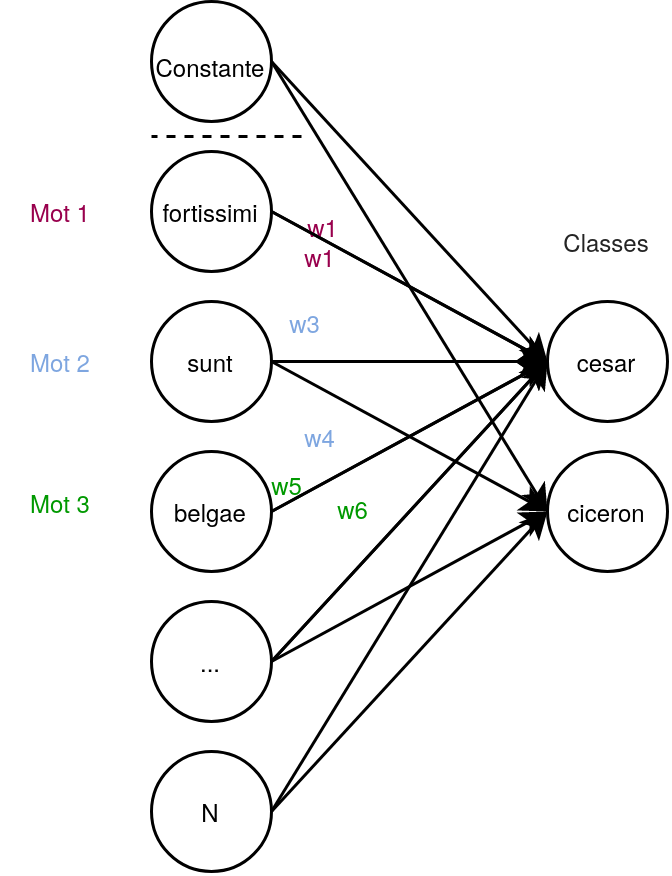
\includegraphics[width=\linewidth]{figures/chap2/SimpleLinear.png}
        \caption{Exemple de couche linéaire (simplifiée)}
        \label{fig:deep-learning:simple-linear}
    \end{minipage}%
    \hspace{0.04\linewidth}
    \noindent\begin{minipage}{.60\linewidth}
        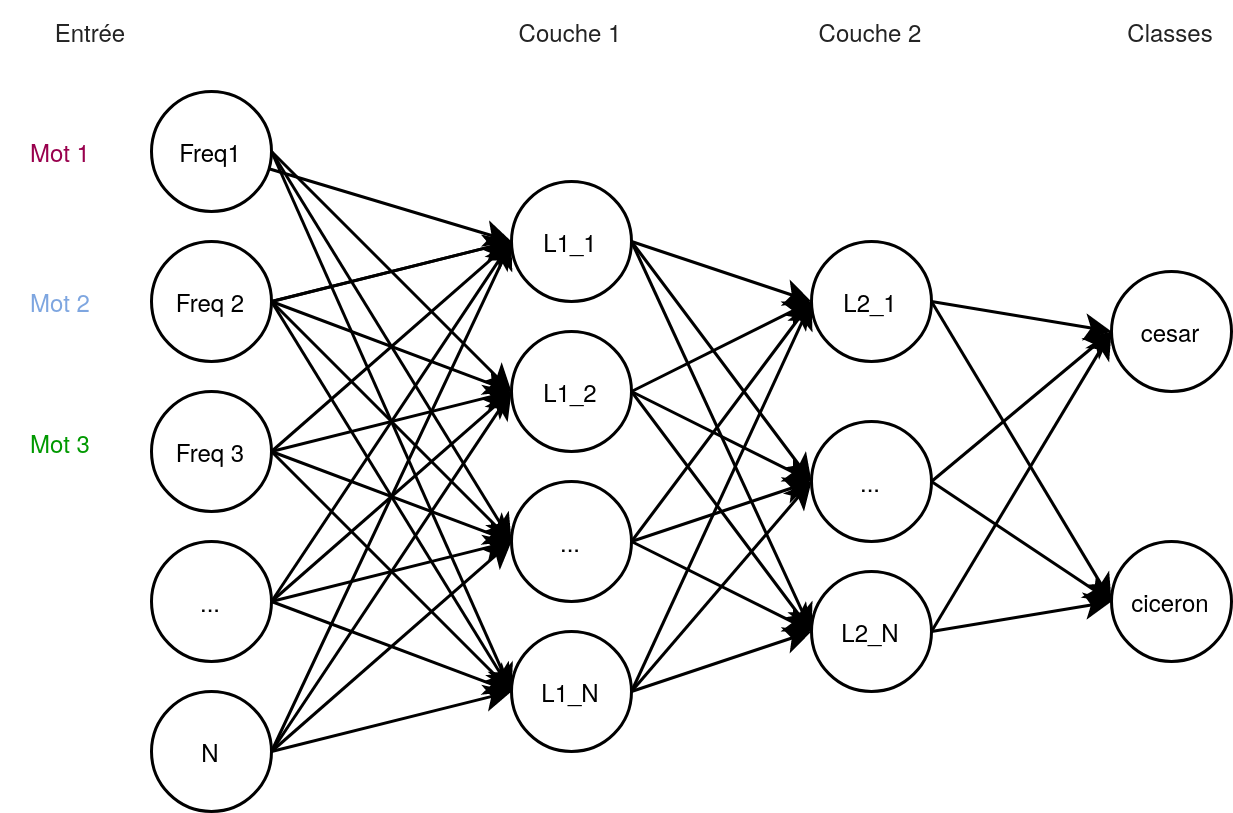
\includegraphics[width=\linewidth]{figures/chap2/MLP.png}
        \caption{Exemple de perceptron multicouche. Le réseau construit ici possède une entrée de taille N, une sortie de 2, et un réseau $Linear(N, L1_N) \rightarrow Linear(L1_N, L2_N) \rightarrow Linear(L2_N, 2)$}
        \label{fig:deep-learning:mlp}
    \end{minipage}%
\end{figure}

Les couches linéaires prennent une forme mathématique très simple. Dans le cadre d'un vecteur de fréquence comme dans la figure \ref{fig:deep-learning:mlp}, le perceptron prend une matrice de taille $M$ par 1 (le vecteur) et ressort une matrice de taille $M...O$ où $O$ est le nombre d'auteurs. Sur ce vecteur, le modèle n'applique qu'une fonction affine. À chaque valeur $M_{i}$ (ici, $i$ est un index de mot), et pour chaque classe de sortie notée $j$, on associe un poids $w_{ij}$ en plus d'une variable partagée par chaque classe appelée \textit{biais} ($b_{j}$) telle que $f(X, j) = W_{j} \dot X + b_{j}$  où X est la matrice de données en entrée de neurone\footnote{En algèbre linéaire, une multiplication de matrice A, de taille N par M, par une matrice B, de taille M par P, résulte en une matrice de taille N par P: une multiplication peut donc réduire la deuxième dimension d'une matrice ou l'augmenter.}.


\section{Réseaux Neuronaux Acycliques (RNN; LSTM et GRU)}

Malheureusement, les couches linéaires posent un problème, en particulier pour les TALs et le traitement d'image: il ne traitent pas vraiment les données en séries. Les perceptrons multicouches ne gèrent l'ensemble des données que comme un ensemble de phénomènes plus ou moins indépendants et, dans tous les cas, non séquentiels. On appelle ce type de réseau \textit{feed-forward} (propagation directe). Pour traiter des données en séries, on s'est d'abord tourné vers d'autres types de réseaux, appelés \textit{réseaux neuronaux acycliques (recurrent neural networks, RNN)}. Les réseaux récurrents ont la particularité de traiter les données en séries, et de réutiliser l'analyse de chaque élément pour l'analyse de l'élément suivant, comme le montre le schéma en \ref{fig:deep-learning:rnn}.

\begin{figure}[h]
    \centering
    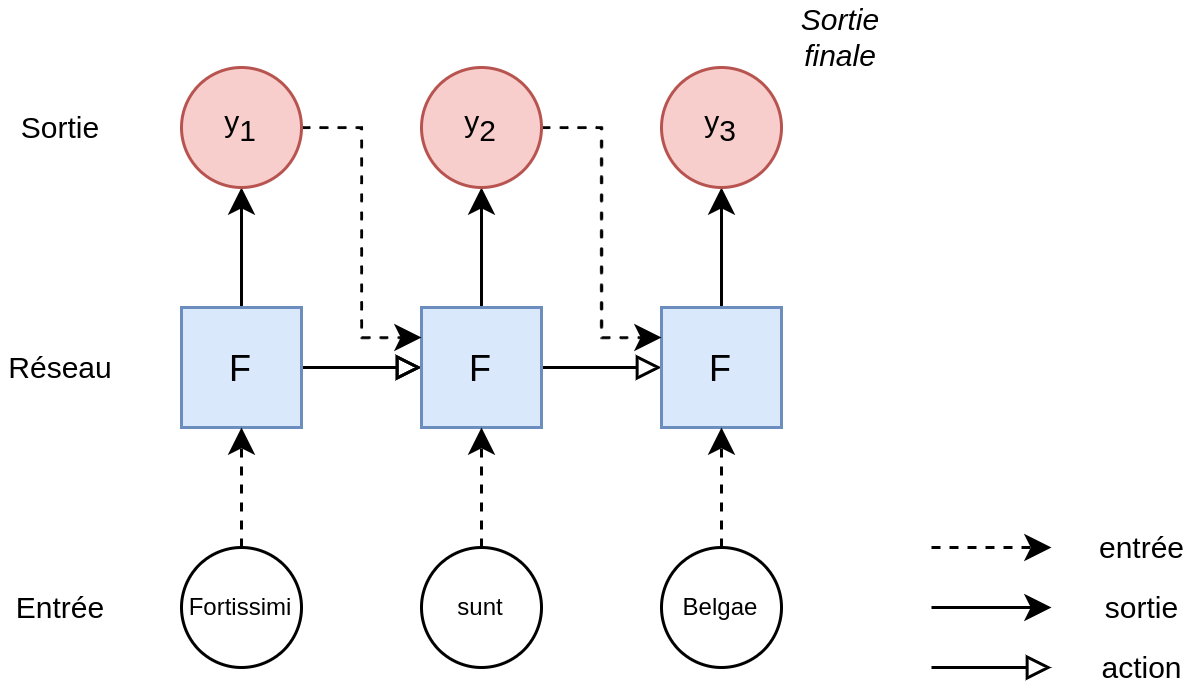
\includegraphics[height=5cm]{figures/chap2/RNN.png}
    \caption{Exemple de réseau acyclique}
    \label{fig:deep-learning:rnn}
\end{figure}

\begin{figure}[h]
    \centering
    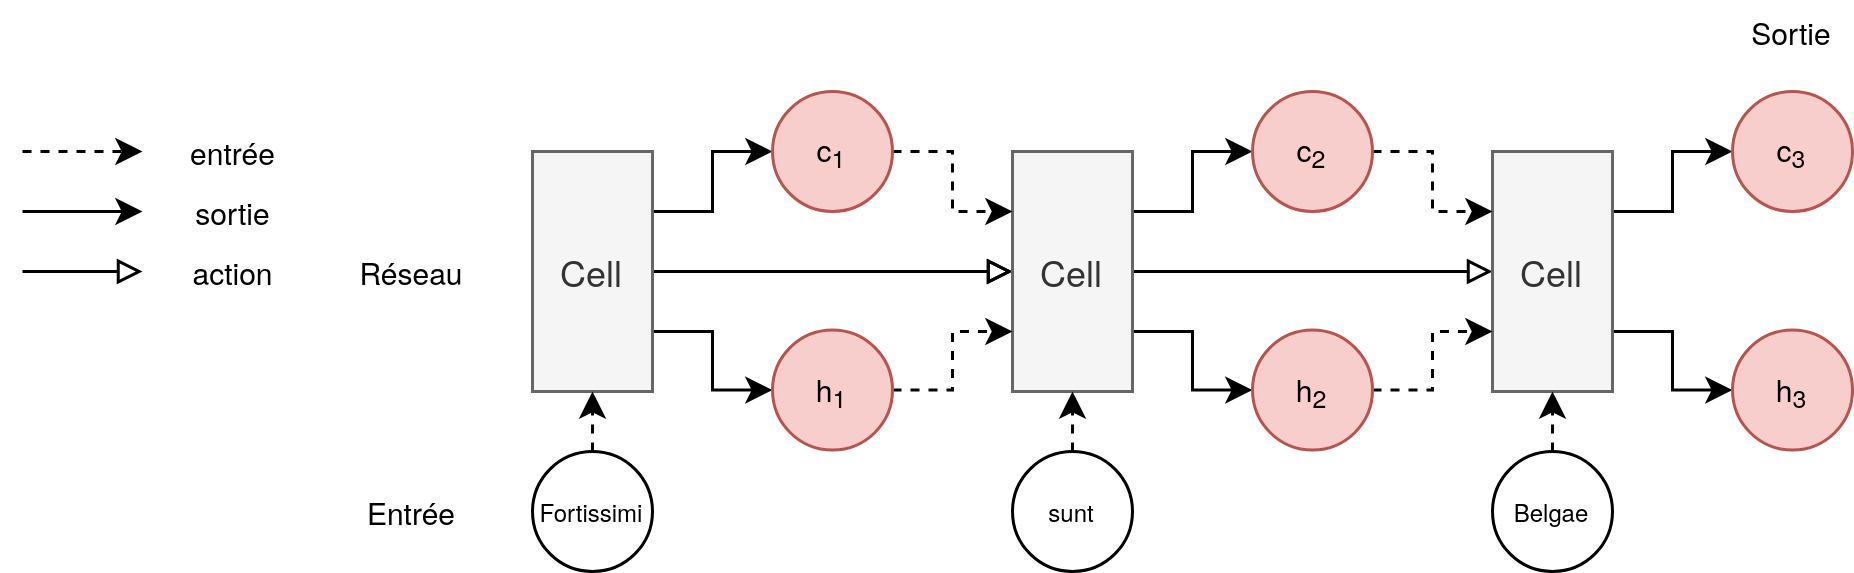
\includegraphics[width=\linewidth]{figures/chap2/LSTM-Zoom-Out.png}
    \caption{Plusieurs cellules de LSTM}
    \label{fig:deep-learning:lstm}
\end{figure}

Le problème des réseaux acycliques classiques se trouve dans la rétropropagation: alors que l'algorithme va propager les informations sur les erreurs rencontrées, cette donnée de correction va peu à peu perdre de sa valeur. En somme, les derniers mots d'une phrase sont plus corrigés que les premiers mots de celle-ci. Pour éviter un tel problème, Sepp Hochreiter et Jürgen Schmidhuber ont proposé les réseaux \textit{Long Short-Term Memory} (LSTM)\footcite{hochreiter_long_1997}. Ils partent du principe que dans une séquence, tout n'est pas nécessaire. Ainsi, dans la phrase "Caesar sum et fortissimi sunt Belgae", si je m'intéresse au narrateur, deux voire trois mots ont de l'importance: \textit{Belgae, sum, Caesar}. Il n'est donc pas nécessaire de s'intéresser à toutes les valeurs... Pour corriger cela, ils introduisent, en plus d'une valeur de sortie (\textit{hidden state}, notée $y$ dans la figure \ref{fig:deep-learning:rnn}, très souvent notée $h$) une mémoire appelée \textit{cell state} (notée $C$). À partir de ces deux valeurs calculées et des valeurs d'entrées, le réseau peut alors effectuer des filtres et prendre en compte les valeurs qui précèdent ou les ignorer. Il existe trois filtres:
\begin{itemize}
    \item la \textit{forget gate}. Elle a pour but de nettoyer la mémoire engrangée dans la \textit{cell state} en fonction de la valeur d'entrée et de l'\textit{hidden state} précédent. 
    \item l'\textit{input gate}. Elle a pour rôle de filtrer dans les valeurs d'entrées celles qui doivent avoir un impact sur la mémoire.
    \item l'\textit{output gate}. En fonction de la mémoire et de la valeur nouvellement acquise de l'\textit{hidden state}, elle décide de supprimer ou non des valeurs de ce dernier.
\end{itemize}
La combinaison de ces trois systèmes aura alors pour effet de créer un environnement propice à la propagation. Cependant, à force d'accumuler dans un sens, de gauche à droite par exemple, on s'est aperçu que le résultat final accordait plus d'importance aux derniers mots qu'aux premiers. Pour corriger cela, on a proposé de faire des LSTM bidirectionnels: pour simplifier, au lieu d'avoir un seul LSTM, deux sont présents et vont dans des sens différents, puis, le résultat final est une simple concaténation des résultats individuels de ces deux LSTMs.

Dans un réseau en LSTM, on a traditionnellement accès à l'ensemble des \textit{hidden states}, qui correspondent à l'encodage des mots. Si, au contraire, on s'intéresse à l'encodage de la phrase, on utilisera en général le dernier état accessible.

\begin{figure}[h]
    \centering
    \includegraphics[height=5cm]{figures/chap2/GRU LSTM.png}
    \caption{Fonctionnement interne d'une cellule GRU et d'une cellule LSTM. Source: \cite{nguyen_illustrated_2019}}
    \label{fig:deep-learning:lstm-gru}
\end{figure}


\label{deep-learning:gru}
Inventés en 2014 par Cho et al.\footcite{cho_properties_2014}, les \textit{Gated Recurrent Unit} (GRU) cherchent à traiter le même problème que les LSTMs. Leur différence consiste principalement dans leur nombre de filtres (2) et dans l'absence de \textit{cell state}, ce qui les rend potentiellement plus rapides. Les deux valeurs de \textit{gate}, \textit{reset} ($R_{t}$) et \textit{update} ($Z_{t}$), sont calculées en fonction de l'\textit{hidden state} précédent $H_{t-1}$ et du X courant $X_{t}$. La \textit{reset gate} est appliquée à l'\textit{hidden state} précédent avant sa prise en compte pour l'\textit{hidden state} suivant, tandis que l'\textit{update gate} permet de filtrer ce qui va être ajouté du calcul sur $X_{t}$ au résultat final ($H_{t}$) et ce qui en échange doit être conservé de l'état précédent $H_{t-1}$.


\section{Réseaux neuronaux convolutionnels (CNN)}
\label{deep-learning:CNN}

Les réseaux neuronaux convolutionnels (\textit{Convolutionnal Neural Network}, CNN) sont des réseaux \textit{feed-forward} qui règlent le problème des perceptrons multicouches. Développés principalement pour le traitement d'images, il approche une image spatialement en analysant chaque pixel avec ce qui l'entoure pour en faire une sorte de résumé. Son résultat peut ensuite passer dans diverses couches de simplification (\textit{ReLU}) ou de réduction (\textit{Pooling}). En traitement automatique des langues, les CNN se distinguent des RNN en ce qu'ils traitent les mots en contexte indépendamment les uns des autres, tandis que les LSTM unidirectionnels par exemple accumulent les informations des mots précédents avec le mot cible, sans prendre en compte les mots à venir.

\begin{figure}[h]
    \centering
    \includegraphics[width=\linewidth]{figures/chap2/CNN.png}
    \caption{Fonctionnement simplifié et visualisation des paramètres d'un CNN.}
    \label{fig:deep-learning:cnn-tal}
\end{figure}

Un CNN est défini par sa taille de sortie, sa \textit{fenêtre}\footnote{Aussi appelé \textit{kernel, noyaux, filtre, filter}, etc.}, une \textit{marge} (\textit{padding}) et un \textit{pas} (\textit{stride}). La marge permet de prendre en compte les mots aux extrêmités de la séquence en proposant des valeurs nulles de remplissage, comme en figure \ref{fig:deep-learning:cnn-tal} (marge de 1). Le pas indique de combien de mots la fenêtre avance: par défaut, elle avance de 1. 

\section{Architectures Encodeur-Décodeurs}
\label{deep-learning:encoder-decoder}

Les architectures encodeur-décodeur (\textit{encoder-decoder} sont des architectures très récentes et qui ont connu en traitement automatique du langage un succès particulier. Les articles qui les ont popularisés, comme \textit{Attention Is All You Need}\footcite{vaswani_attention_2017} ou celui du modèle Bert\footcite{devlin_bert_2019}, datent en général de la toute fin de la décennie 2010-2020. Leur principe repose principalement sur une architecture dans laquelle un ensemble de RNN (en général) va produire une représentation des données en entrée qui est ensuite réutilisée par un second ensemble de RNN dont la tâche est de produire des données en sortie. Cette architecture est majoritairement utilisée dans la génération de texte, que cela soit en traduction automatique ou en légendage d'image. Nous proposons une lecture linguistique du produit en figure \ref{fig:deep-learning:encoder-decoder} où nous comparons le résultat de sortie d'un encodeur à une forme de signifié: désincarné, l'état produit par l'encodeur ne correspond plus à la langue d'entrée et à ses signifiants, mais ne correspond pas non plus encore aux signifiants de la langue de sortie.

\begin{figure}[h]
    \centering
    \includegraphics[width=\linewidth]{figures/chap2/EncodeurDecodeur.png}
    \caption{Proposition d'interprétation d'une architecture encodeur-décodeur dans le cas d'une traduction automatique entre anglais et français.}
    \label{fig:deep-learning:encoder-decoder}
\end{figure}

\chapter{Lemmatisation}
\label{sec:lemmatiseurs}

\section{Introduction}
\label{subsec:lemma_intro}

Afin de traiter un texte et d'établir des statistiques sur celui-ci, il est courant de le lemmatiser. La lemmatisation d'un texte, et \textit{a fortiori} d'un mot, correspond à sa transformation en
%ou bien on "l'associe à"
une forme canonique, le \textit{lemme}. Traditionnellement identique à la forme d'entrée
%nope, le mot vedette
d'un dictionnaire, le lemme permet de rassembler sous une même étiquette l'ensemble des formes fléchies et variations graphiques qu'il peut connaître. Pour le latin, il s'agira de rassembler ensemble \textsc{me} et \textsc{mihi} sous une racine commune \textsc{ego}. Cet étiquetage permet de clarifier le signal statistique en éliminant où cela est nécessaire un bruit inhérent aux langues flexionnelles (voire aux langues dont le système graphique est variable, potentiellement influencé localement, comme l'ancien français ou le latin épigraphique). Son utilisation principale a longtemps eu pour but la capacité à trouver dans un texte les occurrences d'un terme puis a permis le développement plus tardivement de la linguistique de corpus\footcite{mellet2002atouts}.

\subsection{Tâches et définitions générales}

La lemmatisation est donc un effort de traduction d'un texte en un ensemble de formes normalisées, de telle façon qu'\textit{un mot} ne doit connaître qu'une seule annotation de lemme. Notre définition\footnote{On retrouve cette définition partagée par de nombreuses ressources, entre autres \textit{Wikipedia} anglais et français, et dans la plupart des articles et cours d'introduction à la lemmatisation récents. Par exemple, chez \textcite{srinidhi_lemmatization_2020}: \quote{\textit{Both in stemming and in lemmatization, we try to reduce a given word to its root word.}}} exclut \textit{ipso facto} les outils d'analyse du vocabulaire tels que \textit{Collatinus} qui propose pour chaque forme l'ensemble de possibilités de lemme qu'il estime compatible avec la forme. Ainsi, là où \textit{est} est identifié comme \textsc{edo} et \textsc{sum} par \textit{Collatinus}, un lemmatiseur fait un choix unique, lié généralement au contexte et à la probabilité afférente d'apparition de chacun des lemmes possibles à cet endroit.

Enfin, dans le cadre de la lemmatisation, on préfèrera l'utilisation du terme \enquote{\textit{token}} à celui de \enquote{mot}. En traitement automatique des langues, le \textit{token} est un élément dans un ensemble. Au niveau texte, on découpe volontiers ce dernier en séquences plus ou moins indépendantes, généralement des phrases pour les tâches qui nous préoccupent: ainsi, dans ``\textit{II mulieres Gallaeque estis. Romanus sum.}'', nous avons deux \textit{tokens}, ``\textit{II mulieres Gallaeque estis.'}' et ``\textit{Romanus sum.}''. Au niveau inférieur, dans ces unités longues indépendantes, le \textit{token} est un élément qui correspond à la fois aux mots (\textit{mulieri}), aux nombres (\textit{II}), aux enclitiques (\textit{-que}), mais aussi aux signes de ponctuation (\textit{.}). Pour le latin, la tokenisation cherchera donc potentiellement à extraire les enclitiques: \mintinline{python}{"Gallaeque"} se découpera ainsi en \mintinline{python}{["Gallae", "-que"]}\footnote{Cette tâche n'est pas aussi facile que pourrait le laisser deviner cet exemple: pour les lemmes en \textit{-o, -onis} de la troisième déclinaison, le choix entre une forme \textit{Observatione} découpée en \mintinline{python}{["Observatio", "-ne"]} ou conservée telle quel pour représenter un ablatif singulier ne peut se faire qu'en contexte.}. Ce travail est d'autant plus important qu'il peut faire une différence notable dans le cadre de l'annotation: ainsi, identifier \mintinline{python}{"P. Naso."} en un \textit{token} de premier niveau et trois \textit{tokens} de deuxième (une phrase, 3 éléments dont une abréviation, \mintinline{python}{["P.", "Naso", "."]}) plutôt qu'en deux de deux chacun (deux phrases de deux éléments chacune, \mintinline{python}{["P", ".", "Naso", "."]}) induira une rupture de syntaxe, un changement de contexte qui compliquerait la lemmatisation de \textit{Naso} par exemple en \textsc{nasus} le nez plutôt qu'en \textit{cognomen} \textsc{Naso}.


En plus de la lemmatisation, on trouve souvent adjointes deux types supplémentaires  relevant de l'annotation automatique (ou tâches) sur ces \textit{tokens}, basées sur des analyses syntaxiques ou morphosyntaxiques. D'une part, on retrouve très souvent l'annotation des \textit{Part-Of-Speech} (POS). Cette tâche est traitée très rapidement - dès les années 1990 - par les annotateurs automatiques tels que TreeTagger\footcite{schmid1994treetagger}. Les catégories de POS, que l'on pourrait traduire par la notion de nature en français, consistent en un ensemble de catégorisations grammaticales (et non sémantiques) dépendantes des distributions syntaxiques, des fonctions syntaxiques, et enfin des morphologies acceptables\footcite{schachter1985parts}. En traitement automatique du langage, qu'il s'agisse par exemple de stylométrie\footcite{Cafieroeaax5489}, de classification des genres de texte\footcite{feldman2009part}, ou enfin d'analyse de sentiments\footcite{wang2015pos}, les POS ont démontré un réel apport comme variable (\textit{feature}) des données d'entrées de modèles de prédiction. D'autre part, on pourra ajouter à l'annotation une information morphologique ou morphosyntaxique. Elle peut être prise comme un tout (féminin singulier) ou comme un ensemble d'informations indépendantes (féminin; singulier). On distinguera l'information purement morphologique, qui veut que \textit{bonum}, à l'accusatif est un masculin neutre, de l'information morphosyntaxique, qui veut que \textit{bonum virum} est un masculin. En latin, on compte 8 de ces catégories (Cas, Nombre, Genre, Degré, Mode, Temps, Voix, Personne), chacune avec ses valeurs particulières, et une catégorie supplémentaire en cas d'absence de l'ensemble de celle-ci, pour des termes sans morphologie, comme \enquote{ut}. L'usage de ces traits morphologiques comme \textit{features} n'est pas encore très étudié, %
% je crois 
mais on en trouve des exemples dans certaines études sur la reconnaissance d'entités nommées par exemple \footcite[Par exemple]{zirikly2014named}. Leur utilisation comme variable dans notre étude pourrait se révéler utile: en effet, l'intuition voudrait que l'identification des agents (via les cas et la voie des verbes en contexte), de leur genre et enfin les modes verbaux (l'impératif en particulier) puissent apporter des contributions importantes à la classification d'extraits sur le sujet de la sexualité.


\subsection{Une histoire riche, en particulier pour le latin}

La lemmatisation, en latin, possède une histoire particulièrement riche et liée à celle des humanités numériques \footnote{Une majorité des pistes de recherche nous est fournie par la présentation de N.~Perreaux, \textit{cf.} \cite{perreaux_lemmatisation_2019}}. Il ne s'agira pas ici de faire une histoire exhaustive de la lemmatisation et de son application au latin, mais plutôt d'évoquer des continuités et des ruptures amenant à l'état que l'on connait aujourd'hui de la matière.

Il faut noter que les études classiques ont fait usage de la lemmatisation avant le passage à son usage informatique, à travers la création des index et en particulier, dans leur forme la plus ancienne, des concordanciers. M. et R.~Rouse datent l'apparition de ces derniers dans leur forme plus ou moins actuelle au XIII\textsuperscript{e} siècle, à travers les trois concordances verbales de la Bible, à savoir, dans l'ordre chronologique\footcite{rouse_concordance_1984}: celle de Saint-Jacques (\textit{circa} 1235), la concordance anglaise (sans datation connue, sans exemplaire survivant) et une troisième concordance, qui ne saurait être rédigée après 1285. Les auteurs de cette histoire de la concordance attribuent par ailleurs l'apparition de cette forme non seulement au besoin d'enseigner et d'étudier les Écritures, mais aussi de rassembler une pratique apparaissant au cours du XII\textsuperscript{e} siècle de la \textit{concordantia}, qui consistait à adjoindre aux gloses les références d'autres passages de la Bible liés au terme glosé. Quoi qu'il en soit, il apparait dans ces concordances, comme dans les dictionnaires, une vedette (le lemme) avec l'ensemble de ces formes fléchies en contexte. Il faudra attendre le XIV\textsuperscript{e} siècle, puis le XV\textsuperscript{e} siècle pour qu'apparaissent deux autres concordances, l'une sur la Septante grecque, l'autre sur l'Ancien Testament hébreu.

\begin{figure}[h]
    \centering
    \includegraphics[width=\textwidth]{figures/chap3/JonesConcordance.png}
    \caption{Extrait de  \textit{A concordance to the Historia ecclesiastica of Bede} de Jones, Putnam Fennell.}
    \label{fig:chap3:concordance_jones}
\end{figure}

\begin{figure}[h]
    \centering
    \includegraphics[width=10cm]{figures/chap3/histoire/concordanciers.png}
    \caption{Accumulation par dates de concordanciers conservés à la Bibliothèque Nationale de France d'après une recherche sur le catalogue général.}
    \label{lemmatisation:concordanciers}
\end{figure}

Dans le cadre du projet de Roberto Busa, à partir de 1949, on assiste à la première lemmatisation enregistrée numériquement (bien que sur des fiches perforées) via une collaboration avec IBM. Ce travail novateur aura pour but la constitution d'un corpus gigantesque de 11 millions de mots pour une publication vers 1980 de 56 volumes. Cette oeuvre titanesque est d'ailleurs généralement vue comme l'un des projets fondateurs des humanités numériques: Roberto Busa est certainement aux humanités numériques ce que Thucydide et Hérodote sont à l'histoire, dans la méthode du premier comme dans le mythe personnel du second. Cette innovation mécanographique est inédite, mais ne connait pas d'impact direct et immédiat: il faut attendre les années 60 et une  croissance à la fois de l'accès à l'outil informatique (sans parler de démocratisation), de la linguistique de corpus et et de la statistique textuelle (entre autres assistée par ordinateur) pour qu'une suite, ou du moins une méthode parallèle, voit le jour. 

La première occurrence universitaire d'un travail systématique de lemmatisation apparait à l'université de Liège avec le travail du LASLA, fondé le 13 septembre 1961\footcite{delatte_laboratoire_1961}. Dans leur article inaugural, les auteurs Louis Delatte et Étienne Évrard traitent de l'importance de la statistique en matière d'études stylistiques, et, partant du constat que les indices à disposition des chercheurs sont \enquote{incomplets, inexacts ou même inexistants\footcite{delatte_laboratoire_1961}}, ils proposent un travail systématique d'annotation des textes latins et leur enregistrement mécanographique. Tout en portant de nombreuses critiques envers un possible manque de rigueur statistique de certains philologues, cet article montre surtout les opportunités, dans la continuité scientifique des approches du domaine gréco-romain, que porterait un tel outil, à savoir l'assurance de détecter des phénomènes non pas subjectivement ou intuitivement, mais à partir de \enquote{comparaisons entre probabilités théoriques et fréquences réelles}. Par ailleurs, l'article annonce la première étape du laboratoire, à savoir l'annotation des œuvres de Sénèque. La perspective des deux fondateurs du laboratoire est révolutionnaire, et la violence à demi-voilée des propos \footnote{\enquote{Dans combien d'allitérations purement fortuites les commentateurs n'ont-ils pas voulu découvrir les intentions les plus subtiles}, \cite[p.~442]{delatte_laboratoire_1961}} rencontre très rapidement des phénomènes de résistance. Dans une perspective d'histoire du domaine de la lemmatisation, Nicolas Perraux\footcite{perreaux_lemmatisation_2019} a fait resurgir une polémique qui va en ce sens entre Pierre Grimal et Louis Delatte. Aux détours de quatre articles\footcites{grimal_delatte_1964}{delatte_propos_1965}{grimal_index_1966}{delatte_index_1968} dont deux sont des comptes-rendus, les deux philologues engagent une \enquote{guerre franco-belge}\footcite{verdiere_pierre_1970}, initiée par P.~Grimal, tournant autour de trois points principaux:
\begin{itemize}
    \item Sans aucun doute, il y a une question de territoire intellectuel. Nous ne pouvons ignorer que P.~Grimal tend à se positionner comme spécialiste francophone incontesté de Sénèque\footcite{verdiere_pierre_1970}, et, alors qu'il écrit une critique de l'index de L.~Delatte publié en 1962, se prépare aussi à publier le sien. Dans le même contexte, quand L.~Delatte fait une critique de la concordance de l'\textit{ad Marciam} de P.~Grimal (publiée en 1965), il le fait aussi en défense de la publication de son propre index de 1964.
    \item De manière sûre et certaine, il y a un débat sur la question de la concordance, conservant le contexte, contre l'index, répertoriant uniquement les passages de chaque lemme. Cette question de la forme, en dehors de toute méthode, est par ailleurs ravivée en 1979, quand L.~Delatte et deux collègues\footcite{delatte_concordantiae_1979} viennent critiquer la concordance de Sénèque, générée pourtant automatiquement via des fiches mécanographiques, éditée par Roberto Busa.
    \item Enfin, et c'est un problème clair, une résistance complète et totale à la question du numérique de la part de P.~Grimal. L.~Delatte pose un ensemble de jalons importants pendant les années soixante, non seulement en créant la \textit{Revue de l'Organisation Internationale pour l'Étude des Langues Anciennes par Ordinateur} \footnote{Aujourd'hui nommée \textit{Revue du LASLA}. Autrefois abrégée RELO} mais en fondant sa pratique de la mécanographie sur un pilier simple, celui de tout enregistrer pour pouvoir manipuler, statistiquement ou traditionnellement, des données en séries: \enquote{Le document de travail est, pour nous, le fichier de cartes perforées}\footcite[p~.202]{delatte_index_1968}. Au contraire, P.~Grimal se réfugie tour à tour derrière des considérations matérielles (\enquote{D’ailleurs, qui a son ordinateur personnel ?}\footcite[p.~111]{grimal_index_1966}) ou bien une incompréhension des possibilités de l'informatique:
\end{itemize}
    

\begin{quote}{P.~Grimal}
    \enquote{Renoncer à la machine, ce serait aussi se libérer d'un certain nombre de servitudes, comme l'adoption d'un code qui devient rapidement assez complexe lorsqu'on cherche à condenser un grand nombre de renseignements sur une fiche. La machine ne peut connaître que des catégories bien définies, chacune étant traduite par un symbole. Ces catégories constituent comme un quadrillage à l'intérieur duquel le réel doit entrer de gré ou de force, sans déborder d'une case dans l'autre.\footcite[p.~131]{grimal_delatte_1964}}
\end{quote}

Quoi qu'il en soit, si cette polémique, s'étirant sur une dizaine d'années, entre Liège et Paris, nous montre des formes de résistances et des questions quant aux nouvelles formes qui émergent, elle fait aussi ressortir le travail titanesque qui se fait autour de L.~Delatte et É.~Évrard au LASLA. Il est y fait mention d'une \enquote{machine à lemmatiser} dès 1965\footcite{delatte_programme_1965} qui propose pour une forme donnée l'ensemble des lemmes pouvant s'y rattacher, faisant tourner des rouages algorithmiques autour de quatre sets de données: les formes irrégulières, complètes, ne permettant aucune reconnexion (\textit{e.g.} les formes de \textsc{sum} au présent); les radicaux; les terminaisons avec leurs codes morphologiques; les préfixes verbaux (\textsc{ad-sum} par exemple, afin de réduire la taille des calculs.). Cette base d'analyseur morphologique est la même que pour \textit{Words}\footcite{whitaker_words_1993}, \textit{Morpheus}\footcite{crane_generating_1991}, \textit{LEMLAT}\footcite{bozzi_lemlat_1992} ou encore \textit{Analysis}\footcite{ouvrard_analysis_1992} qui devient ensuite \textit{Collatinus}\footcite{ouvrard_collatinus_1999}. Tous ces outils apparaissent au début des années 90, et deux, \textit{Collatinus} et \textit{Words}, sont issus du travail de passionnés, l'un professeur de latin, Yves Ouvrard, et l'autre colonel de l'armée étatsunienne, William Whitaker\footnote{D'après sa nécrologie, il était en effet membre de la \textit{Defense Advanced Research Projects Agency} (DARPA), mais \textit{a priori} retraité au moment de la création de Words. \textcite{noauthor_william_nodate}}.

Cependant, si l'on retient pour lemmatiseur une définition stricte d'annotation d'une forme par un lemme, impliquant un choix en contexte donc, le premier lemmatiseur du latin vient bien plus tard. Et il ne s'agira pas d'un lemmatiseur du latin, mais bien d'un lemmatiseur généraliste: ce que Delatte estimait potentiellement impossible en 1968\footnote{\enquote{Un tel programme, supposant d'ailleurs une analyse conceptuelle, est très difficile sinon impossible à réaliser}, \cite[p.~100]{delatte_index_1968}}, l'augmentation des puissances de calcul et de mémoire vive des ordinateurs a permis de le faire. À partir des années 1990, on voit apparaître des lemmatiseurs prenant en compte le contexte dans le choix des lemmes pour les formes ambivalentes. %(Insertion études par collatinus du nombre de lemme possible par forme ?). 
Pour prendre en compte ce voisinage des mots analysés, on a généralement donné à ces outils des données d'entraînement permettant la reconnaissance de phénomènes lexicaux. Parmi ces outils, TreeTagger a, semble-t-il, reçu les faveurs de la communauté des latinistes des périodes classiques et médiévales, bien qu'il ne soit \textit{a priori} pas le plus performant\footcite[Voir]{eger_lexicon-assisted_2015}. Plusieurs hypothèses peuvent être émises quant à cette situation\footnote{Il faudrait, à ce sujet, probablement faire des recherches et des entretiens plus poussés que ne nous le permet notre sujet ici.}. Il se pourrait que les phénomènes suivants aient fortement influencé sa place actuelle dans le domaine: son incorporation via \textit{TXM}\footcite{heiden:halshs-00549779}, sa prise en main relativement tôt due à son ainesse de presque 10 ans sur certains autres \textit{taggers}, sa facilité d'installation, la constitution de modèles relativement tôt. 


\begin{figure}[h]
    \centering
    \resizebox{\textwidth}{!}{%
    \includegraphics{figures/chap3/histoire/floating-point-operations-per-second.png}%
    }
    \caption{Opération à virgule flottante par seconde (FLOPS) entre processeur traditionnel (CPU) et de carte graphique (GPU). Source: \cite{noauthor_cuda_nodate}}
    \label{lemmatisation:histoire:puissance-gpu}
\end{figure}


Ces lemmatiseurs font face ensuite aux modèles complexes de \textit{deep learning} qui apparaissent au milieu et à la fin des années 2010, grâce à une montée en puissance continue des machines en calcul. En effet, dans un contexte d'amélioration des performances des cartes graphiques et de leurs GPUs (\textit{Graphical Processing Unit}, \textit{cf.} \ref{lemmatisation:histoire:puissance-gpu}), principalement poussée par une consommation en jeux vidéo du grand public\footcite{tanz_how_2017}, les chercheurs ont pu accéder à des machines beaucoup plus puissantes qu'auparavant pour des prix beaucoup plus faibles. En avril 2020, le prix d'une carte graphique professionnelle haut de gamme coûtait encore 7~602€ \footcite{noauthor_pny_2020} contre des prix variant de 1~149 à 1~899€ suivant les marques pour le haut de gamme à destination des particuliers\footnote{C'est sur ce modèle que l'ensemble des entraînements de cette thèse a été produit. \textit{Cf.} \textcite{noauthor_recherche_2020}}, en septembre 2020, ce coût était encore potentiellement divisé par deux chez le même constructeur avec l'arrivée d'une nouvelle génération de cartes graphiques. Cette explosion de puissance et sa démocratisation permettent à de plus en plus de laboratoires de s'équiper, y compris ceux ne relevant pas du domaine des sciences de l'informatique, et aux chercheurs de prototyper de nouveaux modèles, permettant d'obtenir des temps d'entraînement particulièrement réduits\footnote{La très grande majorité des calculs se faisant via opération sur décimaux qui sont plus faciles pour les GPU que les processeurs classiques} et donc d'essayer un plus grand nombre de combinaisons possibles de modèles (en 2017, d'après la figure \ref{lemmatisation:histoire:puissance-gpu}), la différence de puissance est de x4). Parallèlement à cette évolution du matériel, les géants du web investissent dans des librairies de développement telles que \textit{PyTorch} (Facebook) et \textit{Tensorflow} (Google) qui permettent elles aussi de faciliter le prototypage de modèles de prédiction sans avoir à gérer la réimplémentation de modèles mathématiques complexes inhérents à l'apprentissage profond. Ce contexte riche de démocratisation logicielle et matérielle permet à des projets comme Pandora \footcites{kestemont_lemmatization_2017}{de_gussem_integrated_2017} puis Pie\footcite{manjavacas_improving_2019} de naître dans des laboratoires non-spécialistes. 

\section{Les différents types d'outil}

\subsection{Les outils à base de règles (dès 1965)}

Dès 1965 et la création du LASLA donc, L.~Delatte et É.~Evrard cherchent à automatiser, en partie, la lemmatisation et l'annotation morphologique. Ce système semi-automatique, qui vise à proposer des solutions sans y faire un choix, repose sur l'utilisation de plusieurs bases de données (lexicales, morphologiques, affixales, etc.). Ce système fondé sur des bases de connaissances se retrouvent chez quatre autres outils cités plus haut, à savoir \textit{Words} de W.~Whitaker, \textit{Morpheus} de G. R.~Crane, \textit{Collatinus} de Y.~Ouvrard (puis Philippe Verkerk à partir de 2015) ou encore, parmi les plus récents, \textit{LemLat}. À partir d'une base de lemmes, reliée à des bases de radicaux et de flexions, l'outil tente différentes combinaisons pouvant correspondre à la forme analysée: lorsqu'un radical et une flexion acceptée par ce radical s'accordent, un lemme et ses analyses morphologiques sont donnés (\textit{cf.} \ref{lemmatisation:outils:collatinusAlgorythme} et \ref{lemmatisation:outils:collatinusAlgorythme} pour des exemples basés sur Collatinus). Chacun de ces lemmatiseurs est basé sur un dictionnaire différent, reflétant l'état de traditions philologiques propres à des centres de recherche ou à des systèmes éducatifs. En effet, \textit{Word} utilise l'\textit{Oxford Latin Dictionary}, \textit{Morpheus} utilise le \textit{Lewis \& Short}, le LASLA utilise le \textit{Forcellini}, Y.~Ouvrard semble utiliser le \textit{Gaffiot}, \textit{LemLat} utilise principalement le \textit{Georges}. Cette différence pose un problème d'incompatibilité des différents outils. C'est d'ailleurs dans ce cadre que l'ERC LILA s'inscrit en tentant de proposer une réconciliation des différents référentiels de lemmes\footcite{mambrini_harmonizing_2019}. Dans cette catégorie d'outils rentrent aussi les outils à base de dictionnaire de formes comme celui du CLTK\footcite{johnson2014cltk} qui enregistrent pour chaque forme connue les lemmes et les analyses possibles, sans nécessairement chercher l'exhaustivité, et proposent les lemmes correspondant aux formes enregistrées.

\begin{figure}[h]
    \centering
    \resizebox{\textwidth}{!}{%
    \includegraphics{figures/chap3/outils/CollatinusDB.png}%
    }
    \caption{Modèles de données dans Collatinus. Les formes sont générées et analysées à partir des flexions et radicaux, en fonction du modèle. }
    \label{lemmatisation:outils:collatinusDB}
\end{figure}


\begin{figure}[h]
    \centering
    \includegraphics[width=6cm]{figures/chap3/outils/collatinus.png}
    \caption{Algorithme simplifié de Collatinus}
    \label{lemmatisation:outils:collatinusAlgorythme}
\end{figure}

L'avantage principal de ce type d'outils consiste en sa capacité d'ingérer de nouveaux lemmes très facilement. Par exemple, dans Collatinus, \textsc{lascivus} est donné par la ligne \texttt{lascīvus=lāscīvus|doctus|||a, um} où \texttt{a, um} est fourni dans un but lexicographique, mais n'a aucune utilité pour la génération des formes: seul \enquote{\textit{lascivus}} et \enquote{\textit{doctus}} (le modèle de déclinaison) suffisent pour cette partie de l'algorithme. Ainsi, pour ajouter un lemme \textsc{christianus}, au cas où ce lemme tardif n'était pas inscrit dans le \textit{Gaffiot} et donc dans \textit{Collatinus}, il suffirait d'ajouter, scansion omise, \texttt{christianus|doctus|||a, um}. À partir de ce simple ajout, la forme \textit{christiani} serait nécessairement reconnue. Le désavantage de ces outils réside dans leur incapacité à faire le choix dans les analyses possibles, qu'il s'agisse des analyses morphologiques (\textit{lasciva} est-il un nominatif singulier féminin ou un pluriel neutre ?) ou des choix de lemmes (\textit{ita} est-il un adverbe ou la deuxième personne du singulier présent impératif actif de \textsc{ito}).

\subsection{Les outils sur base statistique (1994 et après)}

Au milieu des années 90, mais surtout au début des années 2000 apparaissent les lemmatiseurs et analyseurs de POS tels que \textit{TreeTagger}\footcite{schmid1994treetagger}, mais aussi \textit{TnT}\footcite{brants_tnt_2000} et \textit{StanfordNLP}\footcite{toutanova_feature-rich_2003}. Leurs modèles sont principalement construits sur des structures à base de probabilités d'occurrences de phénomènes en contexte, en intégrant la POS à l'analyse de lemme: on utilise d'ailleurs parfois l'expression \enquote{POS-Tagger} pour nommer ces outils. Pour faire simple, ces analyseurs font usage de dictionnaires avec des fréquences possibles de POS, puis, en fonction d'une séquence de quelques mots (3 ou 4 en général), telle que \enquote{\textit{fortissimi sunt Belgae}} pour \enquote{\textit{Horum omnium fortissimi sunt Belgae}}, ils cherchent à établir l'analyse plus probable, avec des stratégies de décisions et d'éliminations diverses. \textit{TreeTagger} change la donne en 1994 en apportant plusieurs modifications, qui probablement expliquent ses performances sur le latin. D'une part, il constitue un dictionnaire de suffixes en plus du dictionnaire de forme, d'autre part, pour faire face aux \enquote{\textit{ungrammaticalities}}\footcite[p.~2]{schmid1994treetagger} possibles de l'anglais, il attribue une probabilité minimale aux probabilités nulles\footnote{Il n'exclut pas les phénomènes improbables, en corrigeant les probabilités de 0 à 0,00001 par exemple.}. Dans le contexte d'une langue latine à l'ordre des mots non fixe et à la morphologie riche, ces deux facteurs pourraient expliquer une augmentation des scores importants comparés aux modèles précédents.

\begin{figure}[h]
    \centering
    \includegraphics[width=\linewidth]{figures/chap3/outils/treetagger_type.png}
    \caption{Type de fonctionnement des outils de l'époque Treetagger. Une seule représentation des données est prise en compte au moment \enquote{d'un seul} calcul. Il s'agit principalement de modèles statistiques basés sur des probabilités d'apparition de phénomènes.}
    \label{lemmatisation:outils:type-treetagger}
\end{figure}

Le problème évident de ces lemmatiseurs reste aujourd'hui leur relation à un dictionnaire de forme et de lemmes qui ne leur permet pas (\textit{cf.} figure \ref{lemmatisation:outils:type-treetagger}), dans la majorité des cas, de prédire un lemme inconnu ou de gérer plus efficacement une forme inconnue en termes de lemmatisation. Les formes sont traitées telles quelles, ce qui pose, même s'ils prennent en compte des suffixes, rapidement des problèmes pour la lemmatisation ou l'annotation  de la POS dans le cadre du latin (avec des marques flexionnelles telles que \textit{-a} communes à la fois aux noms, aux participes, aux adjectifs, etc.).%exemple ? Vraiment difficile de savoir quoi dire ici...

\subsection{Les outils sur base de traduction (Milieu et fin des années 2010 et après)}

En 2016\footcite{kestemont_initial_2016}, Mike Kestemont propose une première version de Pandora\footcite{kestemont_lemmatization_2017}, un tagueur permettant à la fois la lemmatisation, l'annotation de la POS et des traits morphologiques en contexte. Sa particularité est de cibler le latin, à la fois médiéval et classique, en prenant en compte les difficultés inhérentes de cette langue: d'une part, une morphologie très lourde, beaucoup plus lourde que celle de l'anglais souvent pris comme cible par les développeurs de lemmatiseur; d'autre part, une syntaxe particulièrement libre. Ce travail se base alors sur l'état de l'art en traitement automatique des langues, à savoir des modèles d'apprentissage profond (\textit{deep learning}). Le modèle est constitué d'une couche d'\textit{embeddings}, d'un encodeur LSTM et de plusieurs décodeurs fonctionnant soit sur une base LSTM (pour le lemme), soit sur une couche linéaire (pour les tâches morpho-syntaxique).


\begin{figure}[h]
    \centering
    \includegraphics[width=\linewidth]{figures/chap3/outils/Pie.png}
    \caption{Représentation simplifiée de Pie. L'encodeur n'est utilisé que pour les classifications de mots et à l'entraînement comme support d'entraînement supplémentaire. Lettre par lettre, le lemmatiseur traduit la forme en un lemme. Bien que noté \textit{Embeddings}, le module de projection des caractères prend la forme au choix de CNN ou de RNN en plus d'une couche réelle d'\textit{Embeddings} classiques}
    \label{lemmatisation:outils:pie}
\end{figure}

Ce lemmatiseur est perfectionné par E.~Manjavacas\footcite{manjavacas_improving_2019} qui propose une architecture de code plus souple permettant entre autres de tester plusieurs configurations. Il apporte des nouveautés telles qu'une meilleure gestion des caractères via des \textit{embeddings} en CNN (plus rapide) et la mise à disposition des modèles GRU pour les encodeurs et décodeurs. Le principe reste le même que pour la traduction automatique: quand pour ce dernier domaine on tente de traduire des mots en anglais à partir d'une phrase en français, \textit{pie} et les lemmatiseurs du même genre essayent de traduire chacune des lettres d'un \textit{token} en lettres de son lemme, une à une. De cette manière, il intègre des règles de lemmatisation telles que \textit{$\textrm{-ae} \rightarrow \textrm{-a}$}. Cela signifie aussi que ce lemmatiseur peut avoir tendance à créer des lemmes inexistants, tout en respectant une certaine forme de logique interne: potentiellement, les lemmes ne sont pas les bons, mais correspondent à ce que le lemmatiseur a estimé être une forme logique. % Faire une étude ici ?

\section{Corpus et méthodes d'évaluation}
\label{subsec:lemma_corpus}

\subsection{Les corpus disponibles}

Pour l'entraînement d'outils de lemmatisation, il existe très peu de corpus latins. On en compte quatre pour la période classique, utilisant deux dictionnaires de référence, mais trois référentiels de POS. Ces quatre corpus sont issus des projets Perseus, Proiel, Perseids et du LASLA. À l'exception de ce dernier, il sont tous à l'origine des corpus de treebank et non de lemmatisation: il semble qu'il n'y ait pas eu, historiquement, d'autres projets que ceux du LASLA pour la lemmatisation manuelle du latin classique.

Le corpus \textit{Perseus}\footnote{Aussi connu sous le nom de \textit{Latin Dependency Treebank}} est décrit dans son article programmatique de 2006\footcite{bamman_design_2006}. L'objectif de ce projet d'annotation ne concerne en aucun cas la lemmatisation: le terme \textit{lemma} n'est présent qu'une seule fois dans l'article initial pour près de 4000 mots et 10 pages de rédaction. Il est dirigé par D.~Bamman et G.~Crane puis de G.~Celano et de G.~Crane. Dans les années précédant 2020, l'équipe de G.~Crane s'est majoritairement focalisée sur le grec, qu'il s'agisse de l'expansion du corpus de textes édités ou de textes treebankés, résultant en une stagnation du corpus latin. D'ailleurs, ce corpus est le plus petit des corpus d'équipes (\textit{LASLA, Proiel, Perseus}): au mois d'avril 2020, celui-ci contenait 76~670 tokens, ponctuations et enclitiques compris, et ne comprenait aucune œuvre complète. Sa base de lemmes est dérivée du Lewis \& Short\footcite{shorts_latin_1958}, les POS ne sont pas éditées en contexte, mais la morphologie l'est.

Le corpus \textit{Harrington} est un corpus issu d'une pratique pédagogique de l'annotation du latin\footcite{noauthor_harrington_nodate} via la plate-forme \textit{Perseids}\footcite{almas_perseids_2016}. Il suit les mêmes recommandations en lemme et en morphologie que le corpus de \textit{Perseus}, mais diffère sur la grammaire de dépendance utilisée. Certaines œuvres de \textit{Perseus} sont réannotées avec cette grammaire, réduisant ainsi la taille cumulée des deux corpus. Contrairement au corpus \textit{Perseus}, il est encore en cours de production par les étudiants de D.~Harrington. Au mois d'avril 2020, il contenait 120~029 tokens, enclitiques et signes de ponctuation compris et ne comprenait pas non plus d'œuvre complète. 

Le corpus \textit{PROIEL} est un corpus de projet plurilingue d'étude du \textit{Nouveau Testament} dans les langues indo-européennes anciennes\footcite{haug_creating_2008}. Il suit les mêmes recommandations en morphologie et en lemmatisation que les projets \textit{Perseus} et \textit{Harrington} mais diffère sur ses annotations de POS et sur la grammaire de dépendance utilisée. Corpus toujours en activité, il ne comprend aucune œuvre complète, mais est assurément le corpus le plus important des trois issus du Lewis \& Short. Contrairement aux deux précédents, c'est une collection qui, comme le LASLA, est d'abord un projet fondé par des linguistes et grammairiens avant d'être un produit de chercheurs en littératures ou d'enseignants comme G.~Crane et D.~Harrington\footnote{Nous parlons ici de fondation, G.~Celano étant lui aussi un linguiste.}.

\begin{table}[h]
\centering
\resizebox{\textwidth}{!}{%
\begin{tabular}{l|rrrrrr}
\toprule
        & Tokens             & Ponctuation & Nombre     & Nombre  & Lemmes & Dictionnaire \\ 
        &                    &   comprise  &  d'auteurs &  de textes & uniqes & \\   \midrule
PROIEL  & 225~064            & Non                  & 5                & 6  & 7~246              & Lewis\footnotemark\\
Perseus & 79~670             & Oui                  & 12               & 12 & 6~017              & Lewis \\
Harrington & 120~029             & Oui                  & 9               & 12 &  7~675             & Lewis\\
LASLA   & \textbf{1~630~825} & Non                  & \textbf{18}                 &  \textbf{100+}     & 25~135          & Forcellini \\ \bottomrule
\end{tabular}%
}
\caption{Résumé des informations sur les quatre corpus disponibles. Il existe 137 œuvres au sens du LASLA, mais certaines sont des des découpes inhabituelles, nous préférons donc la notation 100+ ici.}
\label{tab:lemmatisation:corpus-entrainement}
\end{table}
\footnotetext{Légèrement modifié.}

Le corpus du LASLA, qui sera retenu de par sa taille et de par sa diversité, est un corpus dont nous avons précédemment parlé et dont la constitution a commencé dans les années 1960\footcites{delatte_laboratoire_1961}{BodsonCodification1966}. Contrairement aux autres, il ne possède aucun texte à partir du II\textsuperscript{e} siècle de notre ère, ce qui en fait sa plus grande faiblesse. L'apprentissage machine reposant principalement sur le nombre de données et leur variété, il n'était pas envisageable d'utiliser une autre source que celle produite par les philologues belges. Par ailleurs, des essais en début de thèse nous avaient prouvé l'incapacité des modèles à prédire des résultats très fiables à partir des données de \textit{Perseus} ou de \textit{Proiel}: à cause de la taille beaucoup trop faible de \textit{Perseus}, le modèle ne s'entraînait pas assez, tandis qu'à cause des données peu variées de \textit{PROIEL}, il ne connaissait que la \textit{Vulgate} et quelques mots de Cicéron.

\begin{figure}
    \includegraphics[width=\linewidth]{figures/chap3/corpus/tokens_per_year.png}
    \caption{Tokens accumulés, par année, en fonction des corpus latins bruts accessibles en \textit{open access} (\textit{Capitains}) ou du nombre estimé  par le \textit{Perseus Catalog}.}
    \label{fig:lemmatisation:corpus-entrainement}
\end{figure}

\subsection{Le corpus du LASLA: choix d'étiquetage}

Le corpus du LASLA utilisé présente 1~630~825 tokens dans la version à laquelle nous avons accès. Il est constitué de 25~135 lemmes, 1~008 types d'annotations morphologiques (\textit{par exemple}  \texttt{Ablatif Pluriel} et \texttt{Deuxième personne Pluriel Indicatif Parfait Actif}) pour 28 grandes catégories syntaxiques (nom, verbe, préposition, etc.) divisées là où il est possible de le faire en déclinaisons (nom1, nom2, etc.). On trouve dans le corpus de très rares erreurs d'annotation, principalement due à une information partielle, et celles-ci semblent marginales au regard du nombre de \textit{tokens}. Le LASLA a fait le choix d'un étiquetage pour majeure partie morphosyntaxique avec désambiguïsation en contexte, laissant quelques cas d'ambiguïtés quand le doute était suffisamment fort pour que l'annotateur ou l'annotatrice ne fasse pas choix. Nous revenons donc sur deux choix affectant les résultats d'analyse automatique: d'une part l'annotation du genre, d'autre part l'annotation des verbes à formes composées.

\subsubsection{Le cas du genre}

Le LASLA a fait le choix de réserver \enquote{l'indication du genre pour les adjectifs, numéraux, les adjectifs-pronoms, les formes déclinées du verbe, hormis le gérondif}\footcite[p.~27]{BodsonCodification1966} dont la répartition est décrite en table \ref{table:lasla:genders-par-pos}. Ce choix a pour conséquence de laisser le genre des noms inconnus: on ne pourra distinguer, dans le contexte de notre recherche, les noms par leur genre masculin, neutre ou féminin, l'information faisant défaut. On pourrait imaginer un travail de réannotation de tous les lemmes dont la POS est NOM avec leur genre quand il est fixe. Ce travail serait potentiellement riche d'influence sur les statistiques finales. Par ailleurs, le genre, à l'inverse du cas et du nombre, n'a pas été analysé en contexte (c'est-à-dire syntaxiquement), mais hors contexte (c'est-à-dire morphologiquement), ce qui laisse des ambiguïtés comme \textit{bonum} qui est à la fois masculin et neutre à l'accusatif singulier. Dans ce contexte, le LASLA crée trois genres morphologiques additionnels aux genres classiques: le Commun, le Masculin-Féminin et le Masculin-Neutre (dont la répartition dans le corpus d'entraînement est visible en \ref{table:lasla:genders-par-corpus}). L'explication derrière ce choix, disponible dans l'article de Bodson\footcite{BodsonCodification1966}, réside dans un problème technique de 1966, qui risquait de poser un problème d'export. Malheureusement, ce choix, aujourd'hui pourtant possible à résoudre, crée une forme de dette technique pour plus de 300 000 mots. On remarque cependant par alignement avec les formes possibles sur \textit{Collatinus} \footnote{\textit{Cf.} annexes numériques.} qu'une analyse en contexte a été probablement faite à la marge (\textit{cf.} table \ref{table:lasla:genders-alignement}).

\begin{table}[!htb]
    \begin{minipage}[t]{.4\linewidth}
        \centering
        \resizebox{\textwidth}{!}{%
            \begin{tabular}{l|rrr}
            \toprule
                     & PRO    & VER    & ADJ    \\ \midrule
            Com      & 30 004 & 14 841 & 26 384 \\
            Fem      & 37 177 & 16 393 & 34 292 \\
            Masc     & 42 598 & 18 785 & 24 331 \\
            MascFem  & 8 398  & 3 968  & 17 477 \\
            MascNeut & 25 459 & 12 170 & 30 815 \\
            Neut     & 46 479 & 11 151 & 25 381 \\ \bottomrule
            \end{tabular}
        }
        \caption{Répartition des genres par POS}
        \label{table:lasla:genders-par-pos}
    \end{minipage}% \quad
    \hspace{0.19\linewidth} 
    \begin{minipage}[t]{.4\linewidth}
        \centering
        \resizebox{\textwidth}{!}{%
            \begin{tabular}{l|rrr}
            \toprule
                       & Train   & Dev   & Test   \\ \midrule
            Fem        & 77 907   & 986   & 8 971   \\
            Masc       & 76 213   & 925   & 8 576   \\
            Neut       & 73 899   & 993   & 8 119   \\
            Com        & 63 304   & 789   & 7 136   \\
            MascFem    & 26 492   & 322   & 3 030   \\
            MascNeut   & 61 031   & 743   & 6 671   \\
            N/A        & 1 153 885 & 14 788 & 130 465 \\
            \textit{- Dont noms} & 433 117  & 5 634  & 48 840  \\ \bottomrule
            \end{tabular}
        }
        \caption{Répartition des genres par corpus}
        \label{table:lasla:genders-par-corpus}
    \end{minipage} 
\end{table}


\begin{table}[h]
\centering
\begin{tabular}{l|lll}
\toprule
         & MascNeut & MascFem & Com    \\ \midrule
0        & 783      & 653     & 1 478  \\
1        & 219      & 3 863   & 33     \\
2        & \textbf{65 852}   & \textbf{25 155}  & 2 512  \\
3        & 1 591    & 172     & \textbf{67 206} \\ \bottomrule
\end{tabular}
\caption{Nombre de genres possibles par alignement Forme+Cas+Nombre via \textit{PyCollatinus}\footcite[\textit{PyCollatinus} est une traduction en python de \textit{Collatinus, cf. }]{thibault_clerice_2018_1243076}. Les informations qui ne sont pas en gras montrent une différence possible entre une annotation morphologique et morphosyntaxique. Il peut aussi s'agir d'erreurs de \textit{PyCollatinus}.}
\label{table:lasla:genders-alignement}
\end{table}

\subsubsection{Les formes verbales composées et leur annotation}

Un autre choix du LASLA a été d'annoter les participes avec le temps de la forme composée: pour \textit{amatus sum}, \textit{amatus} portera l'information du temps (\texttt{parfait}), du mode (\texttt{indicatif}), de la personne (\texttt{1}) et du genre (\texttt{Masc}) sans porter l'information du cas pourtant présent morphologiquement. Au contraire, \textit{sum} portera la simple annotation de verbe auxiliaire. Cela pose un problème de confusion pour une même forme \textit{amatus} qui peut être annotée comme simple participe parfait passif avec une annotation \texttt{Mode Voix Temps} ajoutée à une annotation \texttt{Genre Nombre Cas}, et une forme amatus (ellipse ou présence de) sum qui elle sera annotée aussi avec \texttt{Mode Voix Temps}, mais sans le triplet \texttt{Genre Nombre Personne}. Dans cette optique, \textit{amatus} peut représenter 6 formes conjuguées hors participes, 7 pour le neutre \textit{amatum} (\textit{cf.} Table \ref{table:amatus_forms}). %
%
% Exemple pour le parfait passif
%
Ainsi, dans la phrase du \textit{De Amicitia} de Cicéron, \enquote{\textit{\textbf{uidetis} in tabella iam ante quanta \textbf{facta} labes primo Gabinia lege biennio post Cassia }}, \textit{uidetis} est annoté à la 2\textsuperscript{e} personne du pluriel indicatif présent actif là où \textit{facta} est annoté à la 3\textsuperscript{e} du singulier subjonctif parfait passif. Si cette approche est particulièrement intéressante dans un contexte d'analyse morphosyntaxique, elle est plus difficile à différencier d'un \textit{facta} nominatif pour un lemmatiseur automatique. Quelle différence en effet peut être faite dans la phrase \enquote{\textit{non oculi tacuere tui \textbf{conscriptaque} uino mensa nec in digitis littera nulla fuit}} (Ovid. \textit{Her}. 2.5.17 sqq.) avec le cas précédent ? % D'ailleurs, n'est-ce pas un raté ??

% Fin d'exemple

\newpara

\begin{table}[h]
\centering
\begin{tabular}{@{}lll@{}}
\toprule
Forme & Mode & Temps \\ \midrule
amatus (sum) & Indicatif & Parfait \\
amatus (eram) & Indicatif & Plus-que-parfait \\
amatus (ero) & Indicatif & Futur antérieur \\
amatus (sim) & Subjonctif & Parfait \\
amatus (essem) & Subjonctif & Plus-que-parfait \\
amatus (esse) & Infinitif & Parfait \\
amatum (iri) & Infinitif & Futur \\ \bottomrule
\end{tabular}
\caption{Annotations possibles pour la forme \textit{amatus} dans le LASLA, hors participes}
\label{table:amatus_forms}
\end{table}

Cette multiplicité d'annotation peut rendre difficile le travail de l'annotation automatique, car elle sous-entend une capacité pour le lemmatiseur de reconnaître les formes au nominatif utilisées de manière adjectivale des formes utilisées comme verbe principal ou verbe subordonné. Nous proposons en \ref{subsec:training:lasla-modification} une analyse de modifications pour une simplification du travail du modèle, en vue de la création d'un modèle morphologique et non morphosyntaxique plus performant.

\subsubsection{Création de lemmes, lexicographie, lexicalisation}

La question de la lexicalisation dans le cadre de la lemmatisation est particulièrement importante, en ce qu'elle peut définir ce qui fait lemme. Doit-on pour autant confondre lexicalisation, création de lemme et création lexicographique ? Au sens original du terme \textit{lemme}, la création lexicographique et celle d'un lemme sont confondues, mais le glissement du dictionnaire vers la base de référentiel permet aussi de distinguer les deux et de faire des choix. Par exemple, dans les données du LASLA, on trouvera les lemmes \textsc{Romani}, les Romains, et \textsc{romanus}, romain en adjectif, quoique le \textit{Forcellini}, dictionnaire source utilisé par le LASLA, ne donne que \textsc{Romanus}, et uniquement dans son \textit{Onomasticon}. Cette distinction se retrouve par ailleurs pour l'ensemble des noms de peuples ou d'habitants. Ce résultat est celui du choix de la primauté de la POS comme séparateur des lemmes: à partir du moment où les formes dans le LASLA sont annotées en fonction d'un couple Lemme-POS intangible, la substantivation d'un adjectif donne lieu à la création d'un lemme et donc d'une nouvelle entrée. L'alternative rejetée est celle d'une annotation de la POS en contexte, quelque soit la POS traditionnelle du lemme: on pourrait ainsi avoir un participe passé substantivé en POS NOMcom, mais avec les traits morphologiques du verbe. Ce choix du LASLA n'est pas évident et peut impliquer, dès lors qu'il y a lexicalisation d'adjectifs substantivés, même dans un cas unique ou du moins réduit, une création de lemmes. De fait, doit-on prendre la lexicalisation, c'est-à-dire d'une certaine manière la prise d'autonomie d'une forme pour un nouvel usage, comme phénomène initiateur de création de lemme ? Cette question est difficile, et le débat peut être complexe. Le défi de la diachronie se pose avec l'annotation, à partir du même référentiel, de faire des choix certains et solides. Cela reste un choix et il est clair que chacune des méthodes a ses avantages, et qu'il reste important de quantifier leur impact en termes de créations d'entrées\footnote{Dans le dictionnaire du LASLA, 12,77\% des lemmes adjectifs peuvent correspondre à des participes et des adjectifs, 12,67\% des adverbes correspondent à des ablatifs de NOMcom, 42,96\% des adverbes correspondent à des instrumentaux en -e ou des formes en -iter d'adjectifs et enfin 23,87\% des lemmes de noms communs peuvent correspondre à des adjectifs substantivés.}.

Il ne s'agit pas pour autant de la seule option visant à limiter le nombre de lemmes ou du moins la possibilité de devoir créer des lemmes à occurrence unique. Parmi les autres choix d'annotation, on peut imaginer, dans le cadre où les adverbes dérivés d'adjectifs ou de noms sont des survivances d'un cas instrumental en \textit{-e} long, d'un ablatif singulier pour les substantifs, de ne pas créer de lemme, mais d'annoter, en quasi-uchronie, sur le lemme supposé d'origine. Serait-il intéressant dans cette situation de répertorier les termes ici sous un cas perdu, étymologique, quand cela est nécessaire, et d'annoter la POS en contexte ? Si ce choix ne semble par exemple pas si facile dans le cas des adjectifs, les substantifs à l'ablatif grammaticalisés du type \textsc{nocte} laissent une part d'interprétation assez forte, la grammaticalisation n'étant pas toujours facilement identifiable\footcite{fruyt_adverbes_2008}, en dehors des cas particuliers de comparatifs qui ne sauraient bien sûr être appliqués à un nom (comme un \textit{noctissime}  %\begin{comment}\footnote{Si l'on revient d'ailleurs à \cite{meillet_levolution_1922}, s'agit-il d'une grammaticalisation qui donne lieu à une nouvelle déclinaison au niveau du degré ou une création par analogie dans ce cas précis ?}\end{comment}
ou bien \textit{magis merito} relevé par Claude Brunet\footcite{brunet_merito_2008}). Le risque de cette méthode est clair: dans une volonté d'annotation presque reconstructionniste, on risque de rendre ce travail, lorsqu'il est manuel, encore plus difficile. Dans les différents degrés de création lexicale, il faut donc différencier les problèmes de reconstruction morphologiques (adjectif adverbialisé ou nom adverbialisé à l'instrumental), les problèmes dus à une POS figée par le lemme à la place d'une annotation en contexte (\textsc{romanus} et \textsc{Romani}). Il existe bien sûr des solutions partielles permettant de conserver les données dans l'état, à savoir de créer une base de connaissances claire connectant ensemble ces prises d'autonomie. C'est entre autres une des missions que s'est attribuées le projet de l'ERC LiLa qui court jusqu'en 2023\footcite{passarotti_interlinking_2020} et pour lequel - par exemple - existe une entrée \textit{merito}. Cependant, au moment de la rédaction, le seul type de relation identifié est celle de \textsc{merito} avec une base de lemme (au sens de dérivation) \textsc{mereo}, bien qu'une relation - peut-être trop faible - \textit{isHypoLemma} existe et relie par exemple \textsc{meritus} et \textsc{mereo/mereor}.

\section{Configurations évaluées et processus décisionnel}

\subsection{Impact du choix d'étiquetage des formes passives ou déponentes composées}
\label{subsec:training:lasla-modification}

Le choix d'annoter des formes simples (les participes) par le temps de la forme composée provoque une difficulté d'apprentissage importante. En retirant du lot les formes adjectivales, le \textit{micro-average} des formes simples est de 97,67 là où la même mesure pour les formes composées stagne à 73,30. Par ailleurs, le \textit{macro-average} et l'\textit{écart-type} montre ces disparités (\textit{cf.} Table \ref{table:lasla:formes-simples-formes-composees})\footnote{Le \textit{micro-average} s'intéresse à la moyenne sur l'ensemble des formes tandis que le \textit{macro-average} se concentre sur la moyenne des scores par catégories (par lemme, par cas).}. La déviation standard des temps simples peut-être majoritairement expliquée par des formes extrêmement rares ou erronées comme l'impératif présent passif (1 occurrence sur le corpus de test, 0 de précision) ce qui appuie l'importance des deux mesures de \textit{micro-} et de \textit{macro-average}. Pour gérer ce problème, on propose de traduire les annotations automatiquement pour ces parfaits: les temps composés utilisant le parfait passif passent en \textsc{Mode-Temps-Voix} à \textsc{Par-Pft-Voix} (où voix correspondra donc à passif, déponent ou semi-déponent). Les modes composés de l'infinitif sont annotés avec le cas, il est donc conservé. Les autres modes passent automatiquement au nominatif et perdent l'annotation de personne. Cette conversion double le nombre de participes futurs, augmente de moitié le nombre de participes parfaits passifs et n'a bien sûr aucune incidence sur les participes présents (\textit{cf.} Table \ref{table:lasla:correction-temps}.) Les résultats (Table \ref{table:lasla:formes-simples-formes-composees}) sont sans appel: l'intégralité des annotations de formes composées (qui correspondent désormais aux participes) connaît un bond de 40 points en \textit{macro-average} et 18 points en \textit{micro-average}. L'écart-type reste fort dans la mesure où certaines classes sont trop rares ou fautives (par exemple, les éléments annotés syntaxiquement comme des participes futurs passifs sont dans leur intégralité des participes parfaits passifs et n'ont pas été touchés par cette modification.). Les classes fautives restantes posent un problème, mais leur poids dans l'entraînement est assez négligeable pour ne pas influer la reconnaissance des participes parfaits passifs, participes futurs actifs et participes présents actifs (Table \ref{table:lasla:main-particips}).

% ToDo: L'annotation de l'auxiliaire ?

\begin{table}[h]
\centering
\begin{tabular}{@{}l|r|lll|lll@{}}
\toprule
                                &         & \multicolumn{3}{l}{Pré-correction} & \multicolumn{3}{l}{Post-correction} \\ \midrule
Précision                       & Support      & Macro    & Écart-Type   & Micro    & Macro     & Écart-Type   & Micro    \\ \midrule
Verbes (hors N/A)               & 39~465        & 65,24   & 39,92        & 93,36    & 90,61     & 22,33        & 96,67   \\
Formes simples                  & 31~254        & 94,17   & 16,79        & 97,80    & 94,17     & 16,77        & 97,86   \\
Formes Composées                & 7~027         & 35,70   & 35,66        & 73,78    & 76,36     & 38,10        & 91,74   \\
- \textit{dont participe}       & 4~946         & 64,30   & 36,10        & 80,87    & 76,36     & 38,10        & 91,74   \\
Formes “adjectivales”           & 1~173         & 90,67   & 15,39        & 92,27    & 93,78     & 05,95        & 94,33   \\ \bottomrule
\end{tabular}
\caption{Précision en fonction des catégories de temps sur la base forme composée/simple et les scores de la table \ref{table:lasla:verb-scores}. Les formes autres correspondent au supin, au gérondif, et à l'adjectif verbal, les formes composées contiennent la catégorie participe.}
\label{table:lasla:formes-simples-formes-composees}
\end{table}

% Check participe futur passif ?

\begin{table}[h]
\centering
\begin{tabular}{l|rrr|rrr}
\toprule
 & \multicolumn{3}{c}{Pré-correction} & \multicolumn{3}{c}{Post-correction} \\ 
 & Test & Dev & Train & Test & Dev & Train \\ \midrule
Par-Fut-Act & 214 & 20 & 1726 & 445 & 46 & 3908 \\
Par-Fut-Dep & 14 & 1 & 121 & 30 & 2 & 209 \\
Par-Fut-Pass & 0 & 0 & 0 & 3 & 0 & 54 \\
Par-Fut-SemDep & 1 & 0 & 13 & 3 & 1 & 28 \\
Par-Perf-Act & 1 & 0 & 2 & 1 & 0 & 2 \\
Par-Perf-Dep & 363 & 32 & 3267 & 653 & 65 & 6203 \\
Par-Perf-Pass & 2927 & 309 & 25334 & 4391 & 526 & 38030 \\
Par-Perf-SemDep & 23 & 5 & 217 & 58 & 11 & 537 \\
Par-Pres-Act & 1210 & 137 & 10935 & 1210 & 137 & 10935 \\
Par-Pres-Dep & 188 & 20 & 1493 & 188 & 20 & 1493 \\
Par-Pres-Pass & 0 & 0 & 1 & 0 & 0 & 1 \\
Par-Pres-SemDep & 5 & 5 & 70 & 5 & 5 & 70 \\ \bottomrule
\end{tabular}
\caption{Résultats sur le décompte de participes des conversions automatiques temps composés vers participe. On remarque a posteriori au moins 2 lignes problématiques (Par-Perf-Act) et (Par-Pres-Pass). Le poids de cette erreur sur un macro-average sera important, mais négligeable sur le micro-average}
\label{table:lasla:correction-temps}
\end{table}

\begin{table}[ht]
\centering
\resizebox{\textwidth}{!}{%
\begin{tabular}{l|rrrr|rrrr}
\toprule
 & \multicolumn{4}{c}{Pré-correction}     & \multicolumn{4}{c}{Post-correction} \\ \midrule
              & Précision & Rappel        & F1-Score & Support & Précision     & Rappel        & F1-Score      & Support \\ \midrule
Par-Fut-Act   &   91      &   89          & 90       & 214     & \textbf{97}   & \textbf{99}   & \textbf{98}   & 445     \\
Par-Perf-Pass &   76      &   83          & 79       & 2927    & \textbf{91}   & \textbf{94}   & \textbf{93}   & 4391    \\
Par-Pres-Act  &   94      & \textbf{98}   & 96       & 1210    & \textbf{95}   & 96            & 96            & 1210    \\ \bottomrule
\end{tabular}{}%
}
\caption{Résultats sur les trois formes principales du participe. En dehors d'un avantage de 2 points sur le rappel des participes présents actifs, tous les autres scores connaissent une augmentation notable, malgré une augmentation nette du nombre de données à tester.}
\label{table:lasla:main-particips}
\end{table} 

\subsection{Méthode(s) d'entraînement et résultats préliminaires}

L'entraînement du lemmatiseur Pie nécessite deux choses: il lui faut d'une part un corpus divisé en trois (d'entraînement, d'évaluation et de test), d'autre part, une série d'hyperparamètres concernant l'architecture du modèle et sa méthode d'apprentissage. Les deux ne sont pas indépendants: un corpus extrêmement riche d'une langue à forte variation morphologique ou orthographique demande \textit{a priori} un réseau plus complexe. Dans un premier temps, nous reviendrons sur l'importance de la connaissance du corpus d'entraînement et des potentielles adaptations qu'il faut faire à la marge. Ensuite, nous parlerons des différentes stratégies appliquées pour obtenir le meilleur modèle et proposerons un retour sur ces méthodes.

\subsubsection{Particularités du corpus et prétraitement}

Le corpus du LASLA présente de nombreuses particularités, propres à son statut de corpus annoté manuellement en vue de l'étude de la langue. C'est un corpus que l'on pourrait qualifier d'éditorialisé: des choix de présentation forts sont faits. Parmi ces choix, 
\begin{itemize}
    \item Le corpus ne présente aucune ponctuation syntaxique (coupure de phrase, marque de dialogue): les seuls signes de ponctuation sont réservés aux abréviations. Les phrases sont manuellement coupées au moment de l'annotation par les éditeurs de données. 
    \item Il utilise des parenthèses et des chevrons pour traiter les formes composées du type \textit{scripti <sunt>} et son inverse \textit{<scripti> sunt}.
    \item Il contient des apostrophes marquant des élisions  telles que \textit{venu'}, et des points pour les abréviations telles que \textit{Tib.}. Plus rarement et uniquement pour les fragments, les points indiquent des manques.
    \item Il n'utilise normalement pas de v minuscule ou de j. Leur présence extrêmement rare étant réservée à des oublis de correction. À l'inverse, on ne trouve pas de U majuscule.
    \item Les majuscules ne sont présentes que pour les noms propres et les adjectifs identifiant des peuples. Aucune majuscule n'est présente pour identifier des débuts de phrases.
    \item Le grec est translittéré en betacode, entouré d'un \$ de chaque côté: \enquote{\textit{Graeci \$pa/qh\$ nominant}} pour \textit{πάθη}.
    \item Certains couples de tokens sont considérés comme relevant d'un seul lemme: \textsc{usu capio}, \textsc{usu verio}, \textsc{res publica}, \textsc{bene dico}, \textsc{bene facio}, etc.
    \item Les lemmes sont désambiguïsés via des indicatifs numériques (de 1 à 5) ou des lettres (A, N) (pour les noms propres ou les peuples).
    \item Les lemmes sont en toute majuscule.
    \item Les nombres romains sont lemmatisés en toutes lettres et ne sont pas normalisés: on trouve ainsi \textit{XIIII} lemmatisé en \textsc{QUATVORDECIM}.
\end{itemize}
Ces particularités demandent un prétraitement important qui a pu varier en fonction des résultats. Pour anticiper ces problèmes, nous avons développé le programme \textit{Protogénie} qui permet de prétraiter un corpus et surtout de garder en mémoire les éléments composant les corpus \textit{train}, \textit{dev} et \textit{test}. Nous proposons donc une chaîne de prétraitement permettant de normaliser les points d'entrée, y compris pour \enquote{simplifier} la tâche d'apprentissage du lemmatiseur. Ainsi, on présente les lemmes en minuscules, sauf pour les noms propres qui conservent une majuscule à l'initiale. Les nombres romains sont traduits en nombres arabes et les lemmes simplifiés en leur équivalent: \textit{XIIII} et son lemme \textsc{QUATVORDECIM} deviennent tous les deux 14. Sur ce point, l'effort de traduction ne relève pas des mêmes mécaniques que pour les autres lemmes: les règles flexionnelles ne sauraient être comparées aux règles de formation mathématique des formes. Or, pour éviter un apprentissage 1 à 1 (forme pour lemme) ou éviter un bruit introduit dans la compréhension du modèle flexionnel, on préfère traiter ces formes différemment, au choix en prétraitant l'information (à force de reconnaissance par règles des nombres romains) ou en conservant comme lemme la forme (\textit{XIII} lemmatisé \textsc{XIIII}). Dans un premier temps, on essaie sur ce point une configuration qui remplace les nombres supérieurs à 3 par 3, conservant ainsi les nombres 1, 2 et 3 et réduisant la taille des \textit{embeddings}. Par ailleurs, ce même outil sert à séparer la morphologie en autant de colonnes nécessaires. Une fois les corpus produits, on applique 3 fonctionnalités supplémentaires: la correction des temps composés (cf. \textit{supra} \ref{subsec:training:lasla-modification}), le recollage des clitiques aux termes qui les précèdent et leur identification dans le lemme afin de faire reposer la responsabilité de cette tâche au lemmatiseur, et enfin, l'ajout aléatoire de majuscules en début de phrases et à certains mots de manière aléatoire afin de déjouer un surapprentissage liant majuscule à l'initiale et noms propres.

\subsubsection{Besoin d'optimisation}

\begin{figure}[ht]
    \centering
    \includegraphics[width=\textwidth]{figures/chap3/entrainement/TrainingDuration96BoxPlot.png}
    \caption{Durée d'entraînement des modèles. Les populations sont les suivantes: (Étape 1, Complète) 50, (Étape 1, Interrompue) 44, (Étape 2, Complète) 11, (Étape 2, Interrompue) 19, (Étape 3, Complète) 11, (Étape 3, Interrompue) 10.}
    \label{fig:lemmatisationTrainingTime}
\end{figure}

Une fois le corpus généré, on peut lancer l'entraînement. \textit{Pie} comporte 97 paramètres dont 13 sont des paramètres d'architecture et 18 des paramètres d'optimisation. E.~Manjavacas nous avait dans un premier temps fourni des paramètres qui lui semblaient corrects, mais nous avons souhaité vérifier leur optimisation. Dans ce cadre, nous avons utilisé deux méthodes. La première est manuelle et consiste à vérifier quelques paramètres, en particulier ceux hypothétiquement clefs, à savoir les dimensions de réseaux et le nombre de couches d'encodage des caractères ou des contextes qui déterminent en partie la capacité à apprendre du réseau. Cette méthode a eu l'avantage de nous permettre de confirmer l'identification de ces paramètres clefs et de prendre en main ces configurations. Puis, la deuxième évaluation fut réalisée avec un outil d'optimisation des hyperparamètres, \textit{optuna}\footcite{optuna_2019}, en trois phases. D'abord, l'identification des paramètres ayant le plus d'impact sur l'apprentissage: cela aura permis d'identifier sur 94 entraînements qu'avant tout autre paramètre, les \textit{learning rates} et éléments de \textit{patience} (délais avant de réduire le \textit{learning rate} ou d'estimer qu'il n'y a plus d'amélioration possible) et de prévention du surapprentissage (\textit{dropout}, ou perte volontaire d'information) ont un impact majeur sur les résultats\footnote{On peut retrouver dans les annexes numériques les trois configurations: étape 1 config-optim-base-optuna.json, étape 2 config-optim-random-optuna.json et enfin config-optim-hidden-optuna.json.}. L'étape 2 a construit sur les meilleurs paramètres de \textit{learning rate} pour évaluer les paramètres d'entraînement. Enfin, une dernière étude a été faite sur la taille optimale de la couche contexte. Ce travail est assez particulier pour le domaine des lettres, car il implique des délais pour obtenir des résultats d'expérience qui ne sont pas pas familiers à la recherche en sciences humaines: en fonction de la complexité de l'architecture, il faut compter jusqu'à 10h d'entraînement (cf. Figure \ref{fig:lemmatisationTrainingTime}) et donc plusieurs jours voire semaines pour l'évaluation simple des meilleurs paramètres\footnote{Les trois étapes cumulées représentent 17 jours et 8 heures de calcul sans interruption.}.


\subsubsection{Résultats et Variance}

Une fois les paramètres supposément optimaux trouvés, on peut lancer une batterie d'entraînements, au minimum 5, sur cette configuration et évaluer les résultats. En effet, un entraînement de \textit{machine learning }est particulièrement influençable par des phénomènes aléatoires, liés à l'initialisation des paramètres et poids, à l'ordre d'apparition des mots, etc., et peut représenter une aberration statistique. Pour l'expérience d'optimisation manuelle, on obtient une médiane des écarts-types à 0,10\% et une moyenne à 0,13\%: sur 18 configurations, on peut donc estimer qu'en moyenne, les résultats de tests seront dispersés à 0,13\% du score moyen. Dans le cadre d'un modèle performant en moyenne à 97,5\%, et à titre d'exemple, cela signifie donc que le modèle peut potentiellement avoir des résultats s'étirant de 97,35\% et 97,65\% sur plusieurs entraînements.

\begin{figure}[ht]
    \centering
    \includegraphics[width=0.7\textwidth]{figures/chap3/entrainement/Variance.png}
    \caption{Distribution des écarts-types d'\textit{accuracy} sur la tâche lemme pour 18 configurations de modèles d'entraînement sur 5 entraînements chacun. On estime alors que les modèles peuvent se retrouver, en cas de distribution parfaite, dans une intervalle de résultats d'environ 0,3\%. Pour plus de détails, \textit{cf.} figure \ref{fig:training_variation_per_model} en annexe.}
    \label{fig:training_variation}
\end{figure}

Avec la dernière configuration, le modèle obtient un score de 97,41\% en lemme sur le corpus de test et de 88,45\% sur les formes inconnues (cf. Table \ref{tab:modelFinalLemmatisation}). Les modèles d'annotations de traits morphosyntaxiques fonctionnent tous particulièrement bien, avec la tâche \texttt{cas} en queue qui plafonne à 92,34\%. En agrégeant les résultats, c'est-à-dire en prenant en compte la validité de l'ensemble des annotations automatiques (lemme, traits morphologiques, POS), on obtient les scores de 85,86\% et de 76,68\% sur les formes connues et inconnues. Ces scores sont plus bas, mais ne changent pas les conclusions précédentes: d'abord, car l'ensemble des tâches ne nous intéressent probablement pas (par exemple le degré ne devrait pas apporter beaucoup à notre travail), ensuite, car le modèle reste très performant, 85,86\% étant particulièrement élevé, surtout sur 169~000 tokens de tests. Par ailleurs, avec ses 85,86\%, le modèle n'est pas si loin des scores les plus bas, à savoir le cas (-7 points au total, -2 points sur les formes qui portent ce trait morphologique) et s'écarte largement d'une probabilité de hasard parfait.

\begin{table}[ht]
    \begin{tabular}{l|rrr}
    \toprule
                    & \multicolumn{3}{l}{Accuracy}                           \\
                    & Formes connues & Formes Inconnues &  Formes Concernées \\ \midrule
    Lemme           & 97,41          & 92,92            &                    \\
    POS             & 96,49          & 92,45            &                    \\
    Genre           & 96,28          & 91,49            &   89,98            \\
    Nombre          & 97,02          & 93,85            &   96,44            \\
    Cas             & 92,34          & 87,37            &   87,84            \\
    Degré           & 98,07          & 93,96            &   93,37            \\
    Mode Temps Voix & 98,35          & 90,80            &   94,44            \\
    Personne        & 99,71          & 98,15            &   98,49            \\ \midrule
    Tâches agrégées & 85,86          & 76,68            &                    \\ \bottomrule 
    \end{tabular}
    \caption{Résultats du modèle final. Les formes concernées sont les formes dont le trait morphologique n'est pas absent: par exemple, l'\textit{accuracy} de 87,84\% en cas correspond au taux de succès pour toutes les formes qui sont annotés pour ce trait morphologique, excluant les formes verbales non participiales, les prépositions, etc.}
    \label{tab:modelFinalLemmatisation}
\end{table}

En fin d'expérimentation, un nouvel algorithme chargé de conduire l'apprentissage d'un réseau neuronal (appelé optimiseur), \textit{Ranger}\footcite{wright_new_2019}, a attiré notre attention. Accompagné d'un autre système de contrôle du \textit{learning rate} qu'une réduction après rencontre de plateau\footnote{Seule option disponible de \textit{pie} au moment de cette découverte.}, \textit{CosineAnnealing}, il proposerait de meilleurs résultats que les deux grands optimiseurs que sont \textit{Adam} et \textit{SGD} (disponibles par défaut dans \textit{pie})\footnote{Nous utilisons le conditionnel ici, car, au moment de la rédaction, aucune publication vérifiée par les pairs n'était disponible sur le sujet.}. Nous implémentons donc à la fois \textit{Ranger}, \textit{CosineAnnealing} et une surcouche permettant d'imposer un délai sans optimisation du \textit{learning rate} que conseille aussi le créateur de \textit{Ranger} et faisons quelques expériences sur les paramètres\footnote{Les paramètres les plus performants rencontrés sont 0,01 de \textit{learning rate}, 10 de délai, 40 de \textit{T\_0} pour \textit{Ranger}}. Après celles-ci, il s'est avéré que l'usage de ces nouveaux algorithmes permettait non seulement de réduire le temps d'entraînement d'environ 40\%, mais aussi de stabiliser les résultats en réduisant la variance tout en obtenant de meilleurs scores\footcite{clerice_allow_nodate} (\textit{cf.} \ref{fig:lemmatisation:optimiseur:ranger}). Cette modification de notre méthode d'entraînement permet ainsi de tirer le meilleur du réseau tout en réduisant le temps nécessaire à des ré-entraînements en cas de modification du corpus.


\begin{figure}[ht]
    \hspace*{-0.05\linewidth}
    \begin{minipage}[c]{0.55\linewidth}
        \includegraphics[width=1\linewidth]{figures/chap3/entrainement/boxplot_accuracy_ranger.png}
    \end{minipage} \hfill
    \begin{minipage}[c]{0.55\linewidth}
        \includegraphics[width=1\linewidth]{figures/chap3/entrainement/boxplot_time_ranger.png}
    \end{minipage}
    \caption{Comparaison des résultats en fonction des optimiseurs, en temps (heure) et en \textit{accuracy}, sur trois couples: \textit{Adam/RLR} étant le système de base de \textit{pie}, \textit{Adam/CosDelayed} utilisant Adam avec un délai d'utilisation de \textit{CosineAnnealing}, Ranger/CosDelayed reprenant ce système avec \textit{Ranger} à la place d'\textit{Adam}. }
    \label{fig:lemmatisation:optimiseur:ranger}
\end{figure}

\subsubsection{Vers une typologie des erreurs}

À la suite de nos entraînements, le modèle produit est évalué sur un jeu de données de test. Ce dernier n'a pas été vu pendant l'entrainement, et garantit donc autant que possible la qualité des résultats et l'absence de surapprentissage sur le corpus d'entraînement. Suite au test, une table des confusions est mise à disposition par \textit{pie} (ex. \ref{lemma:confusion-table}). Cette table permet de mieux comprendre les différentes erreurs que le modèle est capable de faire. Pour un résultat de 97,41\% sur le corpus de test, il reste 4~395 erreurs. Sur ces erreurs, nous avons des problèmes de lemmes homographes tels que \textit{liber} et \textit{Liber}, mais aussi de pluriels lexicalisés tels que \textit{liberi}. Sur 64 apparitions dans le corpus de test de \textit{liber}, on obtient une précision de 92\% et un rappel de 89\%; pour \textit{liberi} et ses 67 apparitions on retrouve respectivement 91\% et 96\%. \textit{liber} l'adjectif est confondu 6 fois avec \textit{liberi} la substantivation et 1 fois avec \textit{Liber} la divinité, à l'inverse, \textit{liberi} est confondu 2 fois avec \textit{liber} et 1 fois avec \textit{Liber}. Si l'erreur \textit{liberi}/\textit{liber} est excusable - on peut même se demander s'il s'agit d'une erreur - on retrouve par ailleurs de vraies erreurs, avec des créations lexicales telles que \textit{pancoristus} à la place de l'attendu \textit{panchrestus} pour la forme \textit{panchresto}. Ce type d'erreur peut être introduit par un bruit involontaire créé par des formes de lemmes étymologiques qui induisent des variations orthographiques comme on en trouve avec \textit{negligens} plutôt que \textit{neglegens} et \textit{paedico} à la place de \textit{pedico}\footnote{Dans le \textit{Forcellini}, on trouve l'explication de l'orthographe sous la formule \enquote{\textit{Prima syllaba sine diphthongo scribitur vitio serioris aevi}} (la première syllabe est écrite sans diphtongue à cause du vice de la période tardive) en citant les orthographes supposées erronées des \textit{Priapea}, mais celles correctes de Catulle (21.4) et Martial (11.94.6, 11.104.17, 7.67.1, 11.99.2). Seulement, aucune des éditions modernes à notre disposition ne donne cette version en \textit{-ae-}, à savoir les éditions de Lindsay (Oxford University Press, 1929) et de Shackleton (Teubner, 1990) pour Martial, de Lafaye (Budé, 1923), de Hermman (Latomus, 1957, p. 103), de Mynors (Oxford Classical Texts, 1958) voire même la \textit{Teubner} de Mueller (1892) pour Catulle. Une recherche sur le \textit{Eagle Inscriptions Search Engine} donne deux attestations en \textit{paedic-}, une au \textit{-a-} restitué, une dont les sources (EDR et EDH) donnent une autre orthographe que celle fournie par Eagle. Au contraire, sur l'EDCS, 66 résultats (certains sont des doublons) donnent la forme \textit{pedic-}, dont le graffiti pompéien CIL 04, 10693 antérieur donc à Martial. S'il s'agissait d'une vraie diphtongue, cette chute de la prononciation de la diphtongue pourrait avoir eu lieu avant Cicéron, \textit{cf.} \cite{sturtevant_monophthongization_1916}. L'autre hypothèse ici est celle d'une étymologie grecque supposée par des lexicographes qui auraient archaïsé de ce fait la forme du lemme.}. Si ce type d'erreur existe pour le couple \textit{liber}/\textit{liberi}, on peut par ailleurs, par un croisement avec les données de collatinus, remarquer que:

\begin{enumerate}
    \item 5,54\% des erreurs sont des lemmes verbes remplacés par leur participe parfait passif et donc une forme adjectivale lexicalisée (type \textit{beo}/\textit{beatus})
    \item 5,57\% sont des verbes remplaçant la forme adjectivale, l'inverse de la situation 1.
    \item 1,16\% sont des verbes dont le participe présent rentre en collision avec le lemme attendu (type \textit{negligens}/\textit{negligo}).
    \item 0,96\% sont des erreurs inversées de 3.
    \item 3,59\% sont des noms partageant leur nominatif avec une forme adjectivale (\textit{liberi}/\textit{liber}).
    \item 6,76\% sont des erreurs inversées de 5.
    \item et enfin, 0,50\% des erreurs sont des verbes passifs lemmatisés en actifs, et 0,66\% correspondent à l'inverse.
\end{enumerate}

\begin{table}[]
\centering
\begin{tabular}{lrlr}
\toprule
Expected & Total Errors & Predictions & Predicted times \\ \midrule
qui      & 289          & quod        & 111             \\
         &              & quis        & 103             \\
         &              & quam        & 39              \\
         &              & quo         & 24              \\
         &              & qua         & 11              \\
         &              & quiuis      & 1               \\
quis     & 174          & qui         & 156             \\
         &              & quo         & 8               \\
         &              & quam        & 5               \\
         &              & quod        & 3               \\
         &              & qua         & 1               \\
         &              & cuius       & 1               \\
quod     & 108          & qui         & 103             \\
         &              & quis        & 5               \\
multus   & 56           & multum      & 37              \\
         &              & multi       & 19              \\
bonus    & 26           & bonum       & 14              \\
         &              & bene        & 8               \\
         &              & boni        & 3               \\
         &              & Bonus       & 1               \\ \bottomrule
\end{tabular}
\caption{Table des confusions générée par \textit{pie}. Nous retenons pour l'exemple les confusions en lemme les plus fréquentes.}
\label{lemma:confusion-table}
\end{table}

Dans un cadre plus large, sur 4~398 erreurs, 2~942 portent sur des tokens ambigus, connaissants donc plusieurs solutions de lemmatisation. 451 erreurs portent sur des lemmes inconnus en phase d'entraînement, mais le faible nombre de ceux-ci ne permet pas d'en tirer de vraies analyses statistiques.

\section{Pie: extensibilité des résultats}

L'entraînement de \textit{pie} sur un corpus test donné nous informe de sa valeur sur le corpus en tant que tel. Se pose la question cependant de la capacité de nos modèles à s'appliquer à un corpus étranger, de quantifier l'impact d'une potentielle spécialisation. Pour étudier cet impact, nous proposons quatre expériences qui permettront d'évaluer l'impact de la taille du corpus d'entraînement, de sa variété en style et en genre, et enfin une étude hors-domaine s'appliquant d'abord à un texte important pour notre corpus, les \textit{Priapea}, puis à des extraits de textes tardifs, le corpus du LASLA s'arrêtant avant la fin du premier siècle de notre ère..

\subsection{Évaluation sur des données hors domaine}
\label{subsec:lemmatisation:hors-domaine}

Si les tests du modèle nous présentent un outil performant, au-delà des 97\% de reconnaissance des lemmes, ils ne nous montrent qu'une face de son usage. En effet, la constitution du corpus de test est faite d'extraits non connus certes, mais issus des mêmes textes que le corpus d'entraînement. Ils ont donc une très forte probabilité de posséder les mêmes caractéristiques en termes de syntaxe, de vocabulaire, de coupes opérées par l'éditeur. Par ailleurs, ils posent un second problème qui est celui de la période couverte par le corpus d'origine, à savoir que l'auteur le plus tardif dans le corpus est Juvénal (127\footcite[p. 320]{zehnacker_litterature_2013}), puis Sénèque (65\footcite[p. 231]{zehnacker_litterature_2013}). Ces données, quand elles sont issues du même corpus et qu'elles sont des fractions des mêmes textes que les corpus d'entrainement et de \textit{dev}, sont appelées \enquote{en domaine} (\textit{in domain}).

On parle en apprentissage machine de données \enquote{hors domaine}, il s'agit de données dont les traits de définitions (auteur, genre, période, style, œuvre, etc.) diffèrent pour tout ou partie des données d'entraînement. Pour cette étude, nous proposons deux corpus hors domaines, l'un constitué de l'ensemble des priapées 1 à 78 d'après la numérotation de Baehrens, l'autre constitué de 10 textes d'auteurs tardifs, majoritairement chrétiens. Les \textit{Priapea} offrent un texte à l'extrême fin de notre corpus en termes de chronologie\footcite{citroni_les_2008} et sont parmi les œuvres non étiquetées les plus portées sur le sexe. Par ailleurs, le style court tout particulier de cet ouvrage offre aussi un grand nombre de sujets différents sur un corpus finalement assez réduit (environ 3~000 mots). Le second corpus\footcite{glaise_2020_corpus_tardif} est constitué d'échantillons de dix-neuf œuvres de dix-sept auteurs, dont les passages (hors ponctuation) comptent \textit{a minima} 500 mots et dont les auteurs s'étendent du deuxième siècle au neuvième de notre ère (Eginhard) avec une concentration plus forte autour du quatrième (cf. table \ref{corpus:glaise:dates}). Si la date de fin de ce corpus est plus tardive que les bornes que nous nous sommes posées, elles permettent d'évaluer tout de même la capacité du modèle à s'étendre dans le temps malgré un entraînement spécifique sur un corpus allant de la république au Haut-Empire, où les marques de la chrétienté sont de fait absentes.

\begin{table}[h]
\centering
\begin{tabular}{l|rrrrrrr}
\toprule
Siècle           & 2 & 3 & 5 & 6 & 7 & 7 & 9 \\ \midrule
Nombre d'auteurs & 1 & 3 & 5 & 4 & 2 & 1 & 1 \\
Nombre de textes & 2 & 3 & 6 & 4 & 2 & 1 & 1 \\ \bottomrule
\end{tabular}
\caption{Répartition par siècle des auteurs et œuvres du corpus Glaise}
\label{corpus:glaise:dates}
\end{table}

\subsubsection{Résultats généraux}

Le modèle propose des résultats convaincants sur une très grande majorité des \textit{Priapea}. La particularité de cette œuvre tient, d'un point de vue statistique, à leur très petite taille: une médiane à 30 mots sur les soixante-seize premiers poèmes et une moyenne à 40 à cause d'individus aberrants tels que le poème 51 (150 mots) et 68 (237)\footnote{Au niveau des quartiles, 25\% des \textit{priapées} font moins de 24 mots, 75\% en font moins de 68. Toutes les tailles ne concernent que les mots, hors ponctuation donc, mais incluant les clitiques.}. L'\textit{accuracy} peut donc grandement varier d'un texte à l'autre, une erreur pouvant représenter au pire une chute de 9\% d'un score\footnote{C'est le cas potentiellement des priapées 13, 59 et 62 dans notre édition.} ou au mieux 0,4\% pour la plus grande priapée. Les résultats restent plus qu'honorables, avec une baisse d'uniquement trois points par rapport au corpus de test principal et une accuracy globale de 94,2\% sur la tâche de lemmatisation (\textit{cf.} table \ref{tab:out_of_domain_global_accuracy} et figure \ref{fig:priapea_varations_boxplot}). Certaines priapées ont des scores particulièrement bas qui ne semblent pas avoir de lien avec leur taille: on notera ainsi les priapées 75 (82 mots, 84\%) et 46 (45 mots, 84\%) qui se trouvent dans la moyenne haute des tailles de poème.

Comme le corpus des \textit{Priapea}, le corpus de latin tardif propose des résultats avec une faible perte, de l'ordre de trois points. L'ensemble des autres annotations performent globalement mieux que sur les \textit{Priapea} (annotation \textit{cas} à 92,9\% contre 89,4\%) ce qui peut potentiellement s'expliquer par la forme poétique et courte des poèmes qui ne laisse pas une grande place à l'erreur. Dans ce corpus, deux textes font office de résultats aberrants, à savoir Jérôme, \textit{In Hieremiam} et Grégroire de Tours, \textit{Historia Francum} qui chutent respectivement à 87 et 88\%. Les textes ont majoritairement la même taille, aux alentours de 500 à 600 mots, avec Commodien, \textit{Instructiones} comme texte le plus court (412 mots) et Augustin, \textit{De Civitate Dei} ainsi que Hilaire de Poitiers, \textit{Tractatus super psalmos} comme textes extrêmement longs\footnote{L'export des textes à corriger ayant allongé les textes involontairement, et l'annotation ayant été corrigée, l'ensemble de ces textes a tout de même été conservé, produisant de fait un écart avec la moyenne de 500 mots.}.

\begin{table}[h]
    \centering
    \begin{tabular}{l|rr|rr}
    \toprule
         Catégorie &  \multicolumn{2}{c}{\textit{Accuracy}} & \multicolumn{2}{c}{\textit{Accuracy} quand applicable} \\
    \midrule    
                {} &  Priapées &    Tardif                  & Priapées &    Tardif                                   \\
    \midrule
             lemma &     94,2 &    94,5                   &   N/A    &    N/A                                      \\
               Deg &     96,8 &    97,5                   &   90,3   &    91,5                                     \\
              Numb &     94,7 &    96,5                   &   94,1   &    96,4                                     \\
            Person &     99,0 &    99,7                   &   96,0   &    99,1                                     \\
Mood\_Tense\_Voice &     96,1 &    97,7                   &   87,0   &    92,3                                     \\
              Case &     89,4 &    92,9                   &   84,1   &    88,0                                     \\
              Gend &     91,7 &    92,8                   &   77,8   &    79,2                                     \\
               pos &     95,0 &    67,6                   &   N/A    &    N/A                                      \\
    \bottomrule
    \end{tabular}
    \caption{Résultat du modèle sélectionné sur le corpus des priapées et de latin tardif. L'accuracy quand applicable désigne la précision de l'algorithme sur les termes qui nécessitent une annotation, en d'autres termes, pour la personne par exemple, seules les annotations sur les verbes sont concernées.}
    \label{tab:out_of_domain_global_accuracy}
\end{table}


\begin{figure}[ht]
    \centering
    \includegraphics[width=0.7\linewidth]{figures/chap3/extensibilite/PriapeaBoxPlot.png}
    \caption{Variation des taux d'erreur sur l'ensemble du corpus des \textit{Priapées}}
    \label{fig:priapea_varations_boxplot}
\end{figure}

\subsubsection{Étude des erreurs}

Si ces chiffres annoncent potentiellement une très bonne nouvelle pour la période tardive et les sujets qui nous intéressent, ne s'attarder que sur l'échelle quantitative macro serait une erreur de taille: 6\% de réponses fausses laissent possible un très grand nombre d'erreurs dont il faut avoir conscience. D'abord, parce que dans un contexte traditionnel de richesse lexicale, la loi de Zipf se retrouvant logiquement dans chacun des corpus, on sait que les termes les plus fréquents représentent une très grosse partie du corpus final. Sur le corpus latin tardif, sur 15~188 formes, 4~908 formes dépendent de 34 lemmes qui apparaissent au minimum plus de 100 fois\footnote{Il s'agit du quantile 0,99 du corpus.}. Parmi ces lemmes, seuls 3 sont des verbes (\textit{sum}, \textit{dico}, \textit{facio}) et 3 des noms communs (\textit{deus}, \textit{dominus}, \textit{filius}); seuls les noms présentent une particularité thématique, les trois verbes étant particulièrement fréquents dans la langue latine en général. Il est fort peu probable que des erreurs arrivent sur des termes comme \textit{de}, \textit{pro} ou encore \textit{ab}. Ensuite, parce que notre corpus tardif global représente au moins la moitié de notre corpus latin pris en compte dans nos recherches, et que l'on ne saurait alors se satisfaire d'une inconnue aussi importante.

Dans un premier temps, nous proposons de regarder quelles POS posent un problème au lemmatiseur. Dans un contexte de distribution normale, une POS représentant 40\% des POS du corpus devrait posséder 40\% des erreurs. Or, en figure \ref{fig:latin_tardif_error_pos}, on remarque nettement que les noms propres (NOMpro) ont une très nette surreprésentation parmi les erreurs, avec des cas extrêmes de plus de 50\% des points d'\textit{accuracy} perdus, mais moins de 5\% des mots du corpus. Si l'on prend un corpus type de 500~mots, et 94\% de succès, on dénombre pour ces cas extrêmes 25 noms propres (5\% du corpus), 30 erreurs (6\% d'erreurs) dont 16 ou 17 sont des noms propres. Pour mesurer cet écart, on propose une mesure $Impact$ définie telle que $\text{Impact}_{pos} = \frac{\text{Erreurs}_{pos}}{\left | \text{Erreurs} \right |} \div \frac{\text{Tokens}_{pos}}{\left | \text{Tokens} \right |}$. Ainsi, un impact médian de 6,84 pour la POS \enquote{nom propre} indique que la proportion d'erreurs sur les noms propres est presque sept fois supérieure à la proportion de tokens qu'elle représente. Bien que les verbes et les noms communs aient une forte responsabilité dans le nombre d'erreurs, les médianes de leur Impact sont respectivement de 1,37. Ces impacts très légèrement supérieurs à 1 ne sont pas anormaux, tant certaines catégories ne représentent aucune erreur malgré une importante fréquence: les prépositions représentent ainsi  7\% en moyenne des corpus contre 0\% des erreurs, il en va de même pour les adverbes négatifs (14\%) et les conjonctions de coordination (7\%).

\begin{figure}
    \centering
    \includegraphics[width=1\linewidth]{figures/chap3/extensibilite/LatinTardifPosErrorBoxPlot.png}
    \caption{Responsabilité des POS dans les erreurs du lemmatiseur sur le corpus tardif.}
    \label{fig:latin_tardif_error_pos}
\end{figure}

Désormais, nous pouvons étudier la catégorie des noms propres de plus près. On peut classer les erreurs dans quatre grandes catégories:
\begin{itemize}
    \item Le lemme n'est pas reconnu comme nom propre, car il est vraisemblablement une personnification d'un nom commun par exemple ou bien qu'il n'est pas reconnu comme tel. On rencontre le premier cas avec \textsc{terra} à la place de \textsc{Terra}, \textsc{mater}/\textsc{Mater}, etc. et le second avec *\textsc{uenus} en place de \textsc{Uenus}, *\textsc{iesus}/\textsc{Iesus}.
    \item Le lemme est pris au pluriel à la place du singulier: c'est un problème commun sur les noms de peuples (\textsc{Graecus} contre \textsc{Graeci}).
    \item Le lemme est issu de la langue grecque ou hébraïque: \textsc{Christus}, \textsc{Israel}, \textsc{Pascha}, \textsc{Dauid}. Sur le corpus entier du LASLA, les occurrences de termes dépendant de la déclinaison grecque ne représentent que 1,1\% des noms, soit 5~585 individus sur environs 487~000. Bien que des noms d'origine grecque puissent suivre des déclinaisons latines comme Christus, on peut s'attendre à de plus grandes difficultés sur les autres termes tant ils ont été peu vus à l'apprentissage.
    \item Le lemme possède une variation graphique latine forte, chose inconnue dans le corpus classique, ainsi on trouve les couples \textit{Bethleem}/\textit{Bethlehem}, \textit{Hierusalem}/\textit{Ierusalem}, \textit{Hiezechiel}/\textit{Ezechiel}, ou encore \textit{Hadrianus}/\textit{Adrianus}.
\end{itemize}

Une fois la catégorie des noms propres analysée, on trouve, en plus de ces cas d'erreurs, les types suivants:
\begin{itemize}
    \item Une erreur sur le choix de racine, à savoir le choix entre le verbe \textit{debeo} et le nom \textit{debitum} par exemple.
    \item Une situation inverse au premier cas des noms propres, à savoir un nom commun pris pour un nom propre et dont la première lettre est ainsi capitalisée.
    \item Une erreur sur une racine reconstruite en adjectif de la première classe (en -us donc) à la place d'un nom, comme pour \textit{prophetia}/\textit{prophetius}.
    \item Un problème de lemme à l'orthographe \enquote{réactionnaire}: dans le corpus des Priapées, on rencontre plusieurs fois l'erreur \textit{pedico} contre l'orthographe \enquote{juste} \textit{paedico} du LASLA.
\end{itemize}

Ces catégories semblent couvrir une très grande partie des erreurs hors pronom et permettent d'éclairer les résultats obtenus, mais aussi de cibler les domaines où le corpus peut être amélioré ou bien là où un correcteur automatique pourrait intervenir, en ciblant par exemple les lemmes d'origine grecque ou hébraïque. Ils ne donnent cependant qu'un éclairage particulier sur le résultat du modèle, mais pas sur sa capacité d'apprentissage et de l'influence du corpus d'entraînement.

\subsection{Étude de l'impact de la taille du corpus sur l'efficacité du modèle}
\label{lemmatisation:extensibilite:tailles}

Pour la première expérience, nous voulons évaluer l'impact de la taille d'un corpus sur les différents éléments de mesure à notre disposition. Nous proposons donc des coupes du corpus LASLA à 1\%, 5\%, 7,5\%, 10\%, 20\%, 40\%, et enfin 80\%. Dans chacun des jeux d'entraînement, on réservera 10\% du résultat de la coupe pour un \textit{set} de développement. La découpe se fait au niveau de chacun des fichiers d'entraînement du LASLA, à savoir un découpage au niveau de l'œuvre (\textit{Carmina} de Catulle) ou à un sous-niveau de celle-ci (César, \textit{Bellum Gallicum}, 1). Chaque séquençage connait alors la même variété d'auteur, la même variété de genre et de thème. Les jeux formés d'extraits pris aléatoirement dans les phrases constituées par le LASLA. Nous mesurons trois tâches, à savoir:

\begin{itemize}
    \item la tâche \texttt{lemma}, qui indique une compréhension du vocabulaire, de la syntaxe et de la morphologie,
    \item la tâche \texttt{POS}, qui indique une compréhension morphosyntaxique
    \item la tâche \texttt{Gend}, qui indique une compréhension de la morphologie.
\end{itemize}

Durant l'entraînement, le modèle principal ayant obtenu les meilleurs résultats sur le corpus global a montré des faiblesses sur les corpus de petite taille. Pour chaque corpus, deux configurations ont donc été testées, une avec un module GRU simple couche (RNN=1) et un module GRU double couche (RNN=2) pour la partie de \textit{character embeddings}. Les résultats (\textit{cf.} Table \ref{tab:percent_corpus_comparaison}) montrent que l'augmentation de la taille du corpus avec une même variété de genres et d'auteurs a un impact fort (plus de 1 point de gagné) jusqu'à l'utilisation de 40 \% du corpus, quelle que soit la tâche, ou presque\footnote{Il existe en effet des valeurs aberrantes pour le genre et la POS au moment du passage de 7,5\% à 10\% du corpus.}. Au contraire, les passages de 40\% à 60\% du corpus et de 60\% à 80\% ne représentent des gains que de 0,23 et 0,46 point respectivement, et donc, un passage de 96,79\% d'\textit{accuracy} pour le corpus à 40\% à seulement 97,48\% pour celui à 80\%, pour un doublement du nombre de tokens annotés utilisés pour l'entraînement, soit une augmentation d'environ 600~000 tokens (passage de 622~238 tokens d'entraînement à 1~226~227).


\begin{table}[]
    \centering
    \resizebox{\textwidth}{!}{%
    \begin{tabular}{ll|rrrrrrrr}
    \toprule
     RNN &  \% Corpus &  Lemme &  $\Delta$(Lemme) &  $\theta$ Lemme &  $\Delta$($\theta$ Lemme) &   POS &  $\Delta$(POS) &  Genre &  $\Delta$(Genre) \\
    \midrule
       1 &     0,010 &  0,741 &     0,000 &    0,725 &       0,000 & 0,791 &   0,000 & 0,851 &    0,000 \\
       1 &     0,050 &  0,889 &     0,149 &    0,858 &       0,133 & 0,887 &   0,096 & 0,902 &    0,052 \\
       2 &     0,075 &  0,921 &     0,031 &    0,855 &      -0,002 & 0,921 &   0,034 & 0,930 &    0,028 \\
       2 &     0,100 &  0,936 &     0,015 &    0,894 &       0,039 & 0,929 &   0,008 & 0,933 &    0,003 \\
       2 &     0,200 &  0,949 &     0,013 &    0,882 &      -0,012 & 0,947 &   0,019 & 0,948 &    0,015 \\
       2 &     0,400 &  0,968 &     0,019 &    0,922 &       0,041 & 0,961 &   0,013 & 0,961 &    0,012 \\
       2 &     0,600 &  0,970 &     0,002 &    0,924 &       0,002 & 0,964 &   0,003 & 0,965 &    0,004 \\
       2 &     0,800 &  0,975 &     0,005 &    0,910 &      -0,014 & 0,966 &   0,002 & 0,970 &    0,005 \\
    \bottomrule
    \end{tabular}}
    \caption{Résultat des tests sur un corpus de test de 140~000 mots représentant 80\% du corpus de test original. RNN correspond au nombre de couches du module d'encodage des caractères. Les mesures de gain entre deux étapes, notées $\Delta$ correspondent à la différence avec le modèle précédent, il faut donc lire \enquote{Le modèle à 80\% du corpus performe 0,46 point de plus que le modèle à 60\% du corpus.}. On ajoute une mesure sur un corpus hors domaine, celui de latin tardif, que l'on désigne dans les colonnes par un $\theta$.}
    \label{tab:percent_corpus_comparaison}
\end{table}

D'après ces résultats, on peut penser que le lemmatiseur apprend \enquote{assez} de la richesse de vocabulaire et de la syntaxe d'un auteur pour s'enrichir jusqu'à environ 40\% de ses textes. Une stratégie de création de corpus pourrait donc se focaliser sur l'annotation d'extraits d'auteurs, plutôt qu'une approche d'annotation complète. Cependant, on peut aussi voir les gains minimes comme de véritables bonds en valeur absolue: si, pour un corpus de 10 millions de tokens, les résultats passent de 96,09\% d'accuracy à 96,97\%, et que ces résultats se retransmettent de manière régulière, le nombre d'erreurs passe de 391~000 à 303~000, soit une chute de 88~000 erreurs. Les progressions en \texttt{POS} et en \texttt{Genre} sont toutes les deux limitées au même titre que celle de lemme. Par ailleurs, lors d'une évaluation sur le corpus de latin tardif, on se rend compte que l'extensibilité connait de grosses variations et y compris des reculs (-0,2 point, -1,2 point, -1,4 point sur les passages 5\%, 20\% et 80\%). Nous ne pouvons ici que faire des hypothèses, et deux semblent plus probables que d'autres. La première consiste à estimer qu'il y a un phénomène aléatoire sur la performance en hors domaine, et que, sur une dizaine d'entraînements, on trouverait majoritairement des modèles améliorant le score précédent. Si cette hypothèse est alléchante, elle n'en reste pas moins assez faible, surtout pour des baisses de 1,4 point en hors domaine, mais une augmentation même faible en test classique: elle serait plus crédible sur un écart de moins de 0,5 point, comme nous avons déjà pu le voir sur d'autres entraînements. La deuxième hypothèse consiste à un surapprentissage sur le corpus d'entraînement: le modèle se surspécialiserait sur le corpus classique, se rendant incapable de reconnaître le corpus tardif. Là encore cette hypothèse pose problème, car elle n'expliquerait pas pourquoi, sur un corpus à 100\%, nos scores rebondissent à plus de 94,5\% (+3 points). Il n'est cependant pas à exclure une savante combinaison des deux phénomènes qui créerait ainsi une chute des plus remarquables.



\begin{comment}
\subsection{Taille et diversité: corpus Perseus}
\label{lemmatisation:extensibilite:perseus}

Nous avons vu en \ref{subsec:treebank_corpora} que le corpus de Perseus pour le treebank, mis en forme pour le projet Universal Dependencies (\Gls{UD}), présente un corpus comprenant peu de textes et peu de mots comparés au corpus du LASLA (26 000 mots contre 1,7 million), mais cependant une variété de style et d'époques assez forte parmi les corpus de ce genre.

\newpara

Pour compléter l'analyse précédente \ref{lemmatisation:extensibilite:tailles}, on reproduit un corpus similaire à celui de Perseus, dans la limite où 4 œuvres présentes dans ce dernier ne le sont pas dans le corpus LASLA, à savoir les \textit{Fabulae} de Phèdres, les \textit{Res Gestae} d'Auguste, la \textit{Vie d'Auguste} de Suétone, la \textit{Vulgate} de Jérôme. On propose de remplacer pour le même nombre de phrases par deux autres œuvres \footnote{Ces œuvres sont mentionnées dans le corpus de Perseus original, mais n'ont pas été nettoyées pour le projet \Glspl{UD})} à savoir les \textit{Fastes} d'Ovides et le \textit{Satyricon} de Pétrone. Le corpus d'entraînement, de développement et de test sont constitués à partir du seul corpus d'entraînement en \ref{lemmatisation:extensibilite:tailles}: les séquences sont prises aléatoirement, sans prendre en compte la position de la séquence dans l'œuvre originale de Perseus, l'équivalent de 10\% et 20\% du nombres de phrases en entraînement sont utilisées pour le corpus spécifique de développement et de test (ci-après \texttt{perseus-test}). Le résultat de cette génération de corpus donne 1361 séquences contre 1334 originellement, mais surtout une forte augmentation du nombre de mots 26 081 contre 18 184 démontrant des tailles de séquences plus grandes dans le corpus LASLA (\textit{cf.} tables \ref{table:perseus-ud:chunks-and-tokens}, \ref{table:lasla:perseus-ud}).  Pour l'évaluation, nous proposons à la fois le résultat sur un corpus \texttt{perseus-test} qui représente la même diversité d'œuvres, mais aussi le corpus test utilisés pour nos mesures. Nous n'évaluons que les tâches \texttt{lemma}, \texttt{pos} et \texttt{Gend} pour les raisons mentionnées plus haut. 

\newpara

% Analyse des résultats

\begin{table}[h]
\centering
\begin{tabular}{lll}
\toprule
 Title                  & Chunks & Tokens \\ \midrule
 Auguste, Res Gestae    & 38     & 708    \\
 Caesar                 & 24     & 352    \\
 Cicero, In Catilinam   & 137    & 1897   \\
 Phèdre, Fables         & 233    & 2397   \\
 Properce               & 224    & 2776   \\
 Salluste, Catilina     & 336    & 4999   \\
 Suétone, Vie d'Auguste & 109    & 2046   \\
 Tacite, Histoires      & 64     & 866    \\
 Virgile, Énéide        & 15     & 142    \\
 Vulgate                & 154    & 2001   \\ \midrule
 Total                  & 1334   & 18184  \\ \bottomrule
\hline
\end{tabular}
\caption{Répartition par œuvres du nombres de séquences et de tokens dans le corpus Perseus UD 2.1}
\label{table:perseus-ud:chunks-and-tokens}
\end{table}

\begin{table}[h]
\centering
\resizebox{\textwidth}{!}{%
\begin{tabular}{l|llll|llll}
\toprule
                  & \multicolumn{4}{l}{Test Perseus}        & \multicolumn{4}{l}{Test LASLA}          \\ 
                  & Accuracy & Précision & Recall & Support & Accuracy & Précision & Recall & Support \\ \midrule
\textbf{Lemma}    &          &           &        &         &          &           &        &         \\
\textit{Tous}     & 0.6550   & 0.2864    & 0.2919 & 5754    & 0.6132   & 0.0990    & 0.0858 & 172968  \\
\textit{Inconnus} & 0.0306   & 0.0094    & 0.0155 & 1534    & 0.7480   & 0.2760    & 0.2438 & 12790   \\
\textit{Ambigus}  & 0.7558   & 0.4873    & 0.5027 & 434     & 0.019    & 0.0035    & 0.0061 & 53069   \\ \midrule
\textbf{POS}      &          &           &        &         &          &           &        &         \\
\textit{Tous}     & 0.8427   & 0.7991    & 0.7482 & 5754    & 0.8183   & 0.6831    & 0.6062 & 172968  \\
\textit{Inconnus} & 0.5913   & 0.0947    & 0.0790 & 1534    & 0.7835   & 0.5866    & 0.5358 & 12790   \\
\textit{Ambigus}  & 0.7672   & 0.5453    & 0.5678 & 799     & 0.5671   & 0.0755    & 0.0691 & 53069   \\ \midrule
\textbf{Gender}   &          &           &        &         &          &           &        &         \\ 
\textit{Tous}     & 0.8637   & 0.8448    & 0.6139 & 5754    & 0.8646   & 0.6315    & 0.4288 & 172968  \\
\textit{Inconnus} & 0.6780   & 0.2043    & 0.1463 & 1534    & 0.6604   & 0.6981    & 0.6698 & 12790   \\
\textit{Ambigus}  & 0.6506   & 0.7027    & 0.6620 & 538     & 0.7067   & 0.1615    & 0.1274 & 53069   \\ \bottomrule
\end{tabular}%
}
\caption{Évaluation d'un modèle linéaire entraîné sur le corpus \texttt{perseus-train} (26 081 tokens, 9 textes) dans Pie contre un corpus test de Perseus et un corpus LASLA plus générique (les modèles avec decodeur plafonnant à 0 pour la tâche \texttt{lemma})}
\label{table:lemmatisation:perseus-scores}
\end{table}

\end{comment}

\subsection{Variation de genre, variation de style}
\label{lemmatisation:extensibilite:prose-vers}

\subsubsection{Mise en place}

Afin d'aller encore plus loin dans l'analyse de l'effet du corpus, nous proposons de reproduire les principes de l'étude de C.~Poudat et D.~Longrée\footcite{poudat2009variations}. Dans cette étude, les auteurs analysent l'impact de l'unicité de genre, de style, chronologique sur l'entrainement de taguer automatiques, en particulier TreeTagger cité plus haut. L'expérience repose sur les comparaisons suivantes:
\begin{itemize}
    \item Style d'ouvrage contre style d'auteur (César, \textit{Bellum Gallicum}; César, \textit{De bello civili})
    \item Style d'auteur contre style de genre (César; Pseudo-César et Salluste)
    \item Style du genre à travers le temps (César, Pseudo-César et Salluste; Quinte-Curce et Tacite)
    \item Style de la prose à l'épreuve des variations génériques (histoire; traités, dialogues)
    \item Style de la prose contre le vers
\end{itemize}{}

Cependant, il nous semble important de dévier sur les corpus utilisés et constitués: les corpus constitués dans le cadre de cette évaluation présentent une très grande variation de taille. Or, dans le contexte d'une modélisation, et de l'impact de ces traits (à savoir genre, style, période), il ne semble pas souhaitable de comparer des entraînements effectués sur 52~000 tokens contre des modèles entraînés sur près de 400~000 tokens\footcite[par exemple, p.~135, 2.~2.~4]{poudat2009variations}. Nous reprenons donc les grandes lignes et constituons 4 sous-expériences.

\begin{itemize}
    \item Une première expérience, sur de petits corpus en vers (environ 90~000 tokens), permettra d'identifier l'impact d'un auteur dans un modèle, ou d'une époque: un corpus double Horace \& Lucrèce (91~555 tokens, 6 œuvres différentes), un Virgile (87488 tokens), un Ovide (95~409 tokens).
    \item Une seconde expérience, sur des corpus plus larges (environ 117~000 tokens), permettra d'étudier l'impact du genre avec deux corpus Sénèque (\textit{Ad Lucilium}, 118~801 tokens; Autres œuvres philosophiques, 117~550 tokens), un corpus mixte théâtre Sénèque et Plaute (115~571 tokens, 16 œuvres), un corpus Cicéron court (116~367 tokens, 2 œuvres), un corpus Tacite (117~552 tokens, 4 œuvres).
    \item Une troisième expérience cherchera à analyser l'impact du mode de rédaction (vers contre prose) sur l'extensibilité des résultats avec un corpus Prose (257 034 tokens, 7 auteurs, 9 œuvres) et un corpus Vers (259 717 tokens, 7 auteurs, 17 œuvres).
    \item Une quatrième expérience portant sur des corpus de 390~000 tokens profitera de la richesse du corpus de Cicéron, en évaluant l'impact de la diversité d'auteurs (corpus divers, 392~402 tokens, 13 auteurs, 24 textes) contre celle de la diversité d'œuvres d'un même auteur (corpus Cicéron Discours, 391~390 tokens, 1 auteur, 44 œuvres)\footnote{On peut retrouver le découpage dans la table en annexe \textbf{A FAIRE}}.
\end{itemize}{}

Les œuvres de test sont toujours prises en hors domaine, à savoir qu'elles ne peuvent pas faire partie des mêmes œuvres que les œuvres d'entraînement. Dans la mesure du possible, elles sont aussi issues de corpus d'auteurs différents (\textit{cf.} Table \ref{table:lemmatisation:extensibilite:test-corpus}) et uniquement des données du LASLA, afin de ne pas introduire de variations d'annotation ou d'édition.

\begin{table}
\resizebox{\linewidth}{!}{%
\begin{tabular}{lll|ll|r|l}
    \toprule
     Auteur & œuvre & Passage & Genre & Tokens & Auteur présent dans corpus \\ \midrule
     César & Guerre des Gaules & 3 & Histoire & 3 637 & Prose \\
     Catulle & Poésie & Complet & Poésie & 13 020 & \\
     Cicéron & De l'Amitié & Complet & Traité & 9 272 & Cicéron Petit \\
     &&&&& Cicéron Discours \\
     &&&&& Prose \\
     Cicéron & Catilinaires & 1 & Traité & 9 272 & \textit{idem} \\
     Quinte Curce & Histoires & 3 & Histoire & 7 175 & Prose \\
     &&&&& Divers \\
     Horace & Épodes & Complet & Poésie & 3 071 & Vers \\
     &&&&& Horace+Lucrèce \\
     &&&&& Corpus Divers \\
     Ovide & Ibis & Complet & Poésie &  4 196 & Vers \\
     &&&&& Ovide \\
     &&&&& Corpus Divers \\
     Salluste & Catilina & Complet & Histoire & 10 598 & \\
     Sénèque & De la brièveté de la vie & Complet & Dialogues & 6113 & Sénèque (Les 3) \\
     &&&&& Prose \\
     &&&&& Divers \\
     Sénèque & Médée & Complet & Tragédie & 5 685 & \textit{idem} \\
     Tacite & Germanie & Complet & Histoire & 5 648 & Prose \\
     &&&&& Tacite \\
     &&&&& Divers \\ \bottomrule
\end{tabular}%
}%
     \caption{œuvres et nombre de tokens pour le test }
     \label{table:lemmatisation:extensibilite:test-corpus}
\end{table}

\subsubsection{Outils de mesure}

Avant d'analyser les résultats, nous devons nous assurer que les variables sont indépendantes, à savoir que les résultats sur deux corpus de tests ne sont pas liés entre eux: le résultat sur un Cicéron n'est pas nécessairement lié au résultat sur Properce. Pour cela, on calcule un $\chi^{2}$ qui, ramené au degré de liberté de notre table, nous donne une valeur $p$ indiquant la probabilité que nos variables soient dépendantes. Pour cela, on calcule une fréquence attendue, ici le nombre de bonnes réponses attendues toutes choses égales par ailleurs, notée $e_{ij}$ où $i$ correspond au modèle d'entraînement parmi $m$ et $j$ le corpus de test parmi $n$:

\begin{equation}
    e_{ij} = \left ( \sum_{i=1}^{m}O_{i} \times \sum_{j=1}^{n}O_{j}  \right ) / \sum_{i=1}^{m}\sum_{j=1}^{n}O_{ij}
\end{equation}

Cette probabilité nous permet ensuite de calculer un degré de magnitude entre la valeur observée et la valeur attendue appelé résidu de Pearson noté $r$ et calculé via la formule

\begin{equation}
    r_{ij} = \frac{O_{ij} - e_{ij}}{\sqrt{e_{ij}}}
\end{equation}

Par exemple, en figure \ref{fig:lemmatisation:longree:poetes}, le nombre de bonnes réponses $O_{Virgile/Eclogues}$ est de 5~224, mais sa probabilité attendue, prenant en compte les résultats du modèle Virgile sur les autres textes et des autres modèles sur le corpus \textit{Eclogiae}, est de 4~884. Son résidu de Pearson est donc de 4,86, ce qui indique un très fort écart à ce qui était attendu.

\subsubsection{Poètes contre poètes}

\begin{figure}[ht]
    \hspace*{-0.05\linewidth}
    \begin{minipage}[c]{0.55\linewidth}
        \includegraphics[width=1\linewidth]{figures/chap3/longreeVariante/LongreeVariante-AccuracyStyleDePoesie-Lemme.png}
    \end{minipage} \hfill
    \begin{minipage}[c]{0.55\linewidth}
        \includegraphics[width=1\linewidth]{figures/chap3/longreeVariante/LongreeVariante-AssocPlotStyleDePoesie-Lemme.png}
    \end{minipage}
    \caption{\textit{Accuracy} en lemme de modèles entraînés sur des poètes avec leurs résidus de Pearson}
    \label{fig:lemmatisation:longree:poetes}
\end{figure}

Les corpus d'entraînement des auteurs Virgile et Ovide ont un effet net (r=49 et r=1,6) sur les corpus de tests des auteurs respectifs. Si l'\textit{accuracy} de Virgile s'en ressent, celle d'Ovide reste globalement basse. Il faut rappeler ici la taille des corpus d'entraînement, seulement 90~000 tokens environ. Au contraire, le corpus mixte Horace et Lucrèce ne semble pas décoller, y compris sur les corpus d'Horace ou de Catulle. Les trois corpus n'ont pas une bonne reconnaissance du corpus prosaïque (César) ou semi-prosaïque (Pétrone). Bien que la \textit{Medea} de Sénèque soit mieux reconnue dans l'ensemble, le résidu de Pearson ne permet pas d'établir une forte corrélation avec un modèle en particulier.

\subsubsection{Style d'auteur, style de genre}

\begin{figure}[ht]
    \hspace*{-0.05\linewidth}
    \begin{minipage}[c]{0.55\linewidth}
        \includegraphics[width=1\linewidth]{figures/chap3/longreeVariante/LongreeVariante-AccuracyStyleDAuteurStyleDeGenre-Lemme.png}
    \end{minipage} \hfill
    \begin{minipage}[c]{0.55\linewidth}
        \includegraphics[width=1\linewidth]{figures/chap3/longreeVariante/LongreeVariante-AssocPlotStyleDAuteurStyleDeGenre-Lemme.png}
    \end{minipage}
    \caption{Accuracy en lemme de modèles avec leurs résidus de Pearson: les corpus d'entraînements ont été élaborés pour permettre d'identifier l'importance de l'auteur et du genre en termes de lemmatisation.}
    \label{fig:lemmatisation:longree:auteurVSforme}
\end{figure}

Dans cette étude, deux prosateurs font face à la prose de Sénèque sous deux formes (ses dialogues et traités d'une part, ses lettres d'autre part) et aux vers de Sénèque et de Plaute. On note tout de suite une nette relation entre \textit{accuracy} et forme, puisque Sénèque a des R et des \textit{accuracies} particulièrement hauts sur Catulle et le théâtre de Sénèque. Au contraire, l'œuvre versifiée de Sénèque ne semble pas mieux comprendre le Sénèque prosaïque que d'autres prosateurs (résultats similaires entre Cicéron, \textit{De Amicitia}, \textit{In Catilinam} et le \textit{De Brevitate Vitae} de Sénèque). L'inverse est aussi remarqué puisqu'aucun des modèles de prose de Sénèque ne réagit nettement mieux que celui de Tacite, en \textit{accuracy} ou en résidu de Pearson. Les auteurs de proses fonctionnent bien sur eux-mêmes et Cicéron ainsi que Tacite fonctionnent particulièrement bien sur Salluste: on peut supposer que l'\textit{In Verrem} et les \textit{Philippicae} de Cicéron, formant le corpus d'entraînement ici, partagent avec Tacite et les \textit{In Catilinam} de Salluste des questions de pouvoir politique, de corruption et - par extension - un vocabulaire et un style assez proche. Au contraire, les œuvres philosophiques de Sénèque ne sont pas assez marquées, et en tout cas trop éloignées du \textit{De Amicitia} dans leur style pour influer de quelque manière. Pour finir, après deux tests, on se rend compte du caractère presque neutre du \textit{Satyricon} de Pétrone qui ne semble profiter ni de la prose ni du vers ni encore de la période, mais qui profite tout de même du passage de 90~000 à 115~000 tokens du corpus d'entraînement.

\subsubsection{Versificateur contre prosateur}

\begin{figure}[ht]
    \centering
    \includegraphics[width=0.7\linewidth]{figures/chap3/longreeVariante/LongreeVariante-AccuracyModeDExpression-Lemme.png}
    \includegraphics[width=0.7\linewidth]{figures/chap3/longreeVariante/LongreeVariante-AssocPlotModeDExpression-Lemme.png}
    \caption{\textit{Accuracy} en lemme de modèles avec leurs résidus de Pearson: chaque corpus est formé uniquement de prose ou de vers.}
    \label{fig:lemmatisation:longree:proseVSvers}
\end{figure}

Avec la troisième expérience, le corpus double en taille, mais présente désormais une unité de forme: celle d'un modèle en prose contre celle d'un modèle en vers. Les résultats sont nets, avec une très forte efficacité du modèle prose sur la prose, en $r$ ou en \textit{accuracy}, avec un écart allant jusqu'à 12~points pour le \textit{Bellum Africanum}. Ici, trois auteurs sont totalement absents  des corpus d'entraînement et doivent retenir notre attention, car, logiquement, le style d'auteur ne joue pas dans les scores: il s'agit de Pétrone, de Salluste et de Catulle (nous excluons le Pseudo-César du \textit{Bellum Africanum} par la proximité stylistique recherchée par l'auteur avec César). Nous notons que si la prose fonctionne bien mieux, les vers ne semblent pas nécessairement surperformer en \textit{accuracy} avec des écarts plus réduits, mais tout de même présents. Encore une fois, le \textit{Satyricon} fait office de frontière, avec l'écart le plus réduit de tout le corpus.

\subsubsection{Diversité des auteurs contre celle d'un auteur}

\begin{figure}[ht]
    \centering
    \includegraphics[width=0.7\linewidth]{figures/chap3/longreeVariante/LongreeVariante-AccuracyDiversiteDAuteursContreDiversiteDAuteur-Lemme.png}
    \includegraphics[width=0.7\linewidth]{figures/chap3/longreeVariante/LongreeVariante-AssocPlotDiversiteDAuteursContreDiversiteDAuteur-Lemme.png}
    \caption{Analyse de l'efficacité d'un grand corpus d'auteur contre une diversité de styles (\textit{Accuracy} en lemme et résidu de Pearson)}
    \label{fig:lemmatisation:longree:divAuteursVSTailleAuteur}
\end{figure}

Sur cette dernière expérience, nous posons la question suivante: dans le cadre d'un modèle entraîné sur un corpus déjà conséquent 390~000 tokens, la diversité des auteurs et des genres prime-t-elle sur celle d'un auteur ? Autrement dit, dans le cadre d'une création de corpus d'entraînement, vaut-il mieux annoter beaucoup d'auteurs, quitte à ne pas chercher à annoter les œuvres complètes, ou bien un seul ? Les résultats, en \textit{accuracy}, sont sans appel: la diversité des auteurs permet de surclasser un corpus uni-auteur sur tous les auteurs hors domaine (Salluste, Catulle, Pétrone), sur les auteurs partagés à l'exception de l'auteur utilisé dans le corpus unifié. Et nous noterons sur ce dernier corpus test que la différence est extrêmement limitée, de 0,01 à 0,02 points malgré une spécification du modèle sur le corpus cicéronien. Enfin, il semble que le \textit{Satyricon} fonctionne enfin mieux en \textit{accuracy} avec un mélange prose et vers, cependant, le $r$ ne nous permet pas de conclure en faveur de cette hypothèse.

\subsubsection{Conclusion}

Sur la base de ces résultats, on distingue les effets suivants:
\begin{itemize}
    \item Le style d'un auteur semble plus déterminant que l'époque de rédaction (figure \ref{fig:lemmatisation:longree:poetes}) ou la diversité en termes d'auteurs (figure \ref{fig:lemmatisation:longree:divAuteursVSTailleAuteur}), y compris quand ce style est copié par des imitateurs. Cet effet tend à se limiter sur des corpus très importants (figure \ref{fig:lemmatisation:longree:divAuteursVSTailleAuteur})
    \item La forme, en particulier poétique, prend le dessus sur le style d'un auteur (figures \ref{fig:lemmatisation:longree:auteurVSforme} et \ref{fig:lemmatisation:longree:proseVSvers}).
    \item La proximité de genre (philosophie, histoire en \ref{fig:lemmatisation:longree:auteurVSforme}) a un impact relativement faible. Mais, cet impact faible est à relativiser avec une possible proximité des thèmes des œuvres sélectionnées pour l'expérience..
\end{itemize}

\section{Modèle LASLA+ et étiquetage du corpus}

Après évaluation des limites du modèle sur le hors-domaine, puis des potentielles influences de composition des corpus d'entraînement, on entraîne un second modèle, \textit{LASLA+}, testé sur le même corpus de test, mais que l'on augmentera des corpus hors domaine ainsi que de la \textit{Vulgate} taguée par \textit{Proiel} alignée semi-automatiquement. Nous revenons alors sur les problèmes d'alignement de corpus, les probables erreurs qui se sont glissées et les difficultés que ce nouveau modèle rencontre. Nous aborderons ensuite la question du prétraitement (\textit{preprocessing}) et de son impact sur la lemmatisation pour finir sur une évaluation rapide du corpus annoté automatiquement, via la recherche de termes posant des problèmes dans le corpus qui nous intéresse.

\subsection{Modèle LASLA+ avec ajout des corpus et alignement de la \textit{Vulgate}}

Notre corpus LASLA ne présente aucun auteur tardif, et donc aucun auteur chrétien. Pour remédier à ce manque, un corpus latin tardif (mais non médiéval) existe et est libre de droits: celui de PROIEL\footcite{haug_creating_2008}. Proiel propose trois textes qui ne font pas partie du corpus LASLA, à savoir la \textit{Vulgate} de Jérôme, le \textit{Peregrinatio Aetheriae} et enfin l'\textit{Opus agriculturae} de Palladius. Pour des raisons de temps et d'optimisation de ce dernier, seule la \textit{Vulgate} a été alignée avec le corpus du LASLA.

On pourrait penser qu'un alignement d'un modèle à l'autre est une tâche simple, d'autant qu'\textit{a priori} le LASLA découpe rarement les lemmes en fonction de leur sens, mais uniquement en fonction de leur POS et leur genre\footnote{On note tout de même \textit{populus1}, le peuple, et \textit{populus2} parmi les exceptions.}. Cependant, un alignement lemma/POS/morphologie requiert de s'assurer que les deux corpus ont le même usage de la morphologie et dans une moindre mesure des POS. Pour les lemmes, l'alignement se fait dans l'ordre suivant:
\begin{enumerate}
    \item Le lemme est présent tel quel dans le dictionnaire du LASLA. L'annotation lemme est donc conservée.
    \item Le lemme existe avec un seul indice de désambiguïsation: il est aligné
    \item Le lemme existe avec plusieurs indices de désambiguïsation, on compare alors les POS, par exemple pour \textit{ad} entre ADV et PRE.
    \item Dans le cas où le lemme ne rentre pas dans ces catégories, on vérifie qu'il n'existe pas sous une autre orthographe, par exemple \textit{adulescens} chez Proiel existe sous \textit{adolescens1} ou \textit{adolescens2} suivant la POS, \textit{excaedo} en \textit{excido1}.
\end{enumerate}

La morphologie nécessite par ailleurs un alignement via la suppression du genre pour les formes qui ne sont ni des adjectifs, ni des pronoms, ni des participes. Ensuite, les genres sont alignés via la déclinaison dont relèvent les adjectifs ou les formes. La morphologie est aussi complétée: les indéclinables ne sont pas analysés ainsi par Proiel (mais plutôt comme des absences de morphologie), ce qui nécessite un réalignement. On finit par normaliser l'orthographe des formes et lemmes pour les couples U/V et J/I puis une première conversion est faite. Si cette étape est itérative, l'objectif reste de réduire au maximum les lemmes à corriger manuellement. Enfin, sur les derniers lemmes, plusieurs centaines, on aligne à la main avec le référentiel du LASLA et on crée des entrées quand le lemme est absent, ce qui est souvent le cas pour les noms propres. Cette dernière catégorie est très importante et démontra une nouvelle difficulté pour l'apprentissage, avec des cas d'hapax comme cette généalogie de \textit{Luc}, 3.23:

\begin{quote}
\enquote{\textit{Et ipse Jesus erat incipiens quasi annorum triginta, ut putabatur, filius Joseph, qui  \\fuit Heli, qui fuit Mathat, \\
qui fuit Levi, qui fuit Melchi, qui fuit Janne, qui fuit Joseph, \\
qui fuit Mathathiæ, qui fuit Amos, qui fuit Nahum, qui fuit Hesli, qui fuit Nagge, \\
qui fuit Mahath, qui fuit Mathathiæ, qui fuit Semei, qui fuit Joseph, qui fuit Juda, \\
qui fuit Joanna, qui fuit Resa, qui fuit Zorobabel, qui fuit Salatheil, qui fuit Neri, \\
\textit{...} \\
qui fuit Sarug, qui fuit Ragau, qui fuit Phaleg, qui fuit Heber, qui fuit Sale, \\
qui fuit Cainan, qui fuit Arphaxad, qui fuit Sem, qui fuit Noë, qui fuit Lamech, \\
qui fuit Methusale, qui fuit Henoch, qui fuit Jared, qui fuit Malaleel, qui fuit Cainan, \\
qui fuit Henos, qui fuit Seth, qui fuit Adam, qui fuit Dei.}}
\end{quote}

Cette présence d'hapax pose un double problème dans la mesure où l'orthographe hébraïque ne se fixe pas par usage, telle \textit{Sarug/Seruch}, ou des formes qui n'existent dans le \textit{Forcellini} ou son appendice \textit{Onomasticon} que dans le corps du texte, tel \textit{Azor}, présent dans l'entrée \textit{Sadoc}.

\begin{table}[]
\resizebox{\textwidth}{!}{%
\begin{tabular}{l|rrr|rrr|rrr|rrr}
\toprule
                & \multicolumn{3}{r}{Tous} & \multicolumn{3}{r}{Tokens connus} & \multicolumn{3}{r}{Tokens Inconnus} & \multicolumn{3}{r}{Tokens Ambigus} \\
Tâche            & Acc    & Pre    & Rec    & Acc       & Pre       & Rec       & Acc        & Pre        & Rec       & Acc        & Pre       & Rec       \\ \midrule
Cas             & 94,64  & 90,38  & 88,82  & 94,86     & 91,05     & 89,56     & 90,18      & 74,51      & 70,96     & 88,53      & 87,46     & 86,19     \\
Degré           & 98,41  & 97,61  & 97,83  & 98,59     & 97,78     & 98,1      & 94,72      & 94,2       & 93,23     & 93,57      & 93,78     & 94,69     \\
Genre           & 97,44  & 94,29  & 93,99  & 97,63     & 94,55     & 94,39     & 93,5       & 90,09      & 88,15     & 91,71      & 92,12     & 92,14     \\
Mode/Temps/Voie & 98,9   & 90,21  & 86,81  & 99,07     & 90,88     & 88,88     & 95,37      & 81,31      & 83,74     & 93,91      & 83,72     & 82,34     \\
Nombre          & 98,12  & 98,1   & 97,92  & 98,26     & 98,24     & 98,06     & 95,3       & 93,68      & 93,33     & 93,87      & 93,83     & 93,33     \\
Personne        & 99,77  & 99,12  & 98,2   & 99,83     & 99,25     & 98,64     & 98,49      & 98,05      & 95,65     & 98,29      & 96,08     & 93,33     \\
Lemme           & 97,32  & 84,41  & 84,09  & 97,72     & 90,53     & 90,52     & 89,23      & 76,31      & 75,96     & 92,56      & 69,62     & 70,3  \\ \bottomrule   
\end{tabular}%
}
\caption{Résultats du modèle LASLA+. Acc=\textit{Accuracy}, Pre=\textit{Précision},Rec=\textit{Recall}.}
\label{tab:laslaplus}
\end{table}

Après cet alignement, on ajoute les données des \textit{Priapea} et du corpus chrétien, nous permettant d'obtenir une plus grande diversité de textes et une plus grande couverture thématique et temporelle et donc lexicale. L'entraînement de ce nouveau modèle obtient un score très légèrement moins bon que le corpus d'origine (\textit{cf.} table \ref{tab:laslaplus}). Il est probable que l'ajout de données dont l'édition n'a pas été traitée de la même manière que les autres données du corpus du LASLA ajoute du bruit: c'est finalement une bonne chose, car cette variété permet aussi de s'éloigner d'un corpus \enquote{parfait} et de se rapprocher \textit{de facto} du corpus que l'on traitera ensuite sur lequel l'intervention humaine, au niveau de la segmentation syntaxique, est minimale.

\subsection{Importance du \textit{pre-processing}}

Nous avons parlé jusque là principalement des méthodes d'entraînement et de l'algorithme responsable de la lemmatisation. Il peut exister un certain nombre de problèmes lorsque l'on passe d'une application sur données éditées - tokenisées à la main au niveau phrase et mot, harmonisées en orthographe, etc. - à des données \textit{in situ}. Cette problématique a déjà été étudiée sur d'autres types de tâches comme la classification de textes\footcite{camacho-collados_role_2018} et montre en général des conséquences - au pire mineures - en termes de résultats. Or, nous avons vu que les données du corpus LASLA possèdent une très forte éditorialisation, allant des normalisations de couple u/v et j/i à l'absence de ponctuation, qui, dans le cas d'une lemmatisation \textit{in situ}, influencerait probablement la lemmatisation. En effet, dans la phase de transcodage de \textit{pie}, toute lettre inconnue - comme v par exemple - est codée \textit{de facto} en tant que lettre inconnue et non en tant que v, puisqu'elle n'a pas pu avoir de représentation apprise dans l'espace de projection des caractères. Il faut donc s'assurer que ces lettres, lorsqu'une alternative est possible, sont traduites, remplacées. Du côté de la ponctuation, le choix est tout autre: il faut pouvoir s'appuyer sur la ponctuation pour les tâches telles que la reconnaissance des phrases ou celles des abréviations, mais s'assurer qu'elles disparaissent pour la phase de lemmatisation pure puis réapparaissent pour les futures étapes de notre recherche. D'autres cas, comme la présence de formes grecques ou de nombres, sont indiqués et simplifiés afin d'éviter au lemmatiseur d'apprendre à lemmatiser le grec ainsi que les chiffres romains en chiffres arabes, chose faisable par un programme simple, car extrêmement régulé, mais plus difficile pour un réseau neuronal avec très peu d'exemples.

\begin{table}[ht]
    \centering
    \resizebox{\linewidth}{!}{%
    \begin{tabular}{l|rrrr}
    \hline
                                              & A                 & B                 & C              & D              \\ \hline
    Normalisation des lettres                 & Non               & Oui               & Non            & Oui            \\
    Suppression des formes inconnues (points) & Non               & Non               & Non            & Oui            \\
    Tokenisation Phrase                       & Ponctuation Forte & Ponctuation Forte & 35 Mots        & 35 Mots        \\ \hline
    lemma              & \textbf{-1,51} & -0,22          & \textbf{-1,62} & -0,23 \\
    Deg                & -0,30          & -0,16          & -0,26          & -0,06 \\
    Numb               & -0,41          & -0,31          & \textbf{-0,56}          & -0,12 \\
    Person             & -0,05          & 0,00           & -0,06          & -0,03 \\
    Mood\_Tense\_Voice & -0,11          & -0,02          & -0,12          & -0,04 \\
    Case               & \textbf{-0,76} & \textbf{-0,66} & \textbf{-1,41} & \textbf{-0,32} \\
    Gend               & -0,28          & -0,13          & -0,23          & -0,11 \\
    pos                & \textbf{-0,57} & -0,33          & \textbf{-0,66} & -0,18 \\ \hline
    \end{tabular}}
    \caption{Impact de la normalisation sur l'\textit{accuracy}, en \%.}
    \label{tab:lemmatisation:normalisation}
\end{table}

Dans ce cadre, on propose une expérience assez simple: à partir des données de latin tardif, qui contiennent une orthographe \textit{in situ} et une ponctuation, on fait varier le contenu à lemmatiser en fonction de trois variantes combinables:
\begin{itemize}
    \item Une normalisation des lettres et formes, principalement u/v et j/i,
    \item Une suppression pour l'étape de lemmatisation de la ponctuation et des formes inconnues comme le grec,
    \item Une tokenisation du texte sur la base de la ponctuation forte (points, guillemets, parenthèses, etc.) ou sur une fenêtre de 35 mots. Cette fenêtre est la fenêtre proposée par défaut par \textit{pie}. Plusieurs fenêtres raisonnables (multiples de 5 jusqu'à 35) ont été testées ici, mais elles présentaient des résultats dans des marges minimales.
\end{itemize}
Les résultats, visibles en table \ref{tab:lemmatisation:normalisation}, montrent un fort impact de la conservation des signes de ponctuation et des lettres inconnues avec des scores baissant de 1,51\% à 1,62\% quand les deux sont ignorés. Il faut noter que la conservation des lettres inconnues a - semble-t-il - un impact assez limité (-0,22\%). Au niveau des tâches auxiliaires, toutes les tâches sont touchées sauf la reconnaissance de personne, le cas et la POS étant particulièrement influencées avec des baisses allant jusqu'à -0,76\%. Dans le cadre où la tokenisation des phrases est faite tous les 35 mots, la lemmatisation, le cas et la POS sont légèrement influencées aux alentours de -0,20\%. On note ici que l'accumulation de bruit n'est pas de l'ordre de l'addition: plus le nombre de régularisations manquantes croît, plus les tâches sont influencées. Si les signes de ponctuations ont été supprimés des calculs d'\textit{accuracy} dans l'expérience précédente, nous pouvons retrouver aussi les bizarreries que crée la lemmatisation de signes totalement inconnus tels que dans l'\textit{incipit} de la \textit{Bellum Gallicum} (cf. figure \ref{quote:lemmatisation:gallia-errors}). Dans une telle situation, il est clair que le prétraitement est inséparable d'une bonne lemmatisation via des réseaux neuronaux.

\begin{figure}[ht]
    \begin{quote}[\textit{Bellum Gallicum}]{César}
        \textbf{Source}\\
        \enquote{Gallia omnis divisa in partes tres , quarum unam incolunt Belgae , aliam Aquitani tertiam , qui ipsorum lingua Celtae nostra Galli appellantur.}\\
        \textbf{Lemmatisation brute}\\
        \enquote{gallia omnis \textbf{dico} in pars tres \textbf{qvi} qvi vnvs incolo belgae \textbf{vnde} alivs aqvitani tertivs \textbf{vi} qvi ipse lingva celtae noster galli appello \textbf{nonvs}}\\
        \textbf{Lemmatisation avec normalisation}\\
        \enquote{gallia omnis divido in pars tres , qvi vnvs incolo belgae , alivs aqvitani tertivs , qvi ipse lingva celtae noster galli appello .}\\
        
    \end{quote}
    \caption{Exemple de bruit causé dans la lemmatisation lorsqu’ aucun prétraitement n'est effectué. En gras les erreurs introduites par la lemmatisation: on remarque qu'en dehors de la lemmatisation des points qui est totalement erronée, \textit{divisa} est aussi mal analysé, certainement à cause du bruit de ponctuation et de la lettre v.}
    \label{quote:lemmatisation:gallia-errors}
\end{figure}


%\subsection{Étiquetage du corpus: exploration et différences entre le modèle LASLA et le modèle LASLA+}
 
%Dans cette section, nous ne proposons pas une étude aussi poussée que celles en, \ref{subsec:lemmatisation:hors-domaine} mais une analyse rapide des différences de résultats sur quelques termes qui ont montré des limites pour nos modèles.
\clearpage
\section*{Conclusion}

Entre les premiers concordanciers et la mécanisation de leur production, sept siècles se sont écoulés. En revanche, le concordancier aura ensuite été rapidement dépassé. L'évolution technologique résultant de l'informatisation d'abord, de sa démocratisation croissante et de la progression exponentielle des puissances de calculs a permis d'aborder les textes latins sous de nouveaux angles: celui du quantitatif linguistique d'abord, et celui de l'annotation automatique ensuite.

Dans les années 1960, il serait présomptueux de voir dans le travail du LASLA autre chose qu'une approche systématique de la linguistique latine, déjà bien suffisante pour l'époque. Cette ambition, qui dépasse le cas d'un seul auteur, a permis en une soixantaine d'années de couvrir une part importante du corpus classique. Tout en assurant un équilibre et une variété inégalée dans les genres et auteurs représentés, ce corpus a atteint plus d'un million et demi de mots hors ponctuation. Ce travail a pu nourrir des travaux quantitatifs des équipes du laboratoire producteur des données, mais aussi faire naître des collaborations avec d'autres, comme pour le lancement d'Hyperbase à Nice.

Mais c'est bien l'ouverture des données du LASLA qui a changé radicalement le paysage de la lemmatisation latine. En novembre 2018, lors de l'atelier international \textit{Text Encoding: Latinists looking for new synergies} organisé au LASLA, Dominique Longrée et Margerita Fantoli convient différents acteurs des humanités numériques latines (membres de l'ERC LILA, Bridget Almas d'Alpheios, Philipp Roelli de \textit{Corpus Corporum}, etc.). Cette ouverture et cet événement ont eu des répercussions sans précédents dans le champ d'étude. Plusieurs institutions, toutes avec leurs propres objectifs et approches des corpus, ont alors à leur disposition le plus grand corpus de latin classique intégralement annoté.

Sans cet apport, le travail présenté ici n'aurait probablement pas connu les mêmes succès. Les tests sur les lemmatiseurs connus, à partir des corpus limités de \textit{Perseus} ou de \textit{Proiel}, ne présentaient alors pas une qualité suffisante d'annotation pour traiter en intégralité notre corpus massif. Nous ne pouvons que souligner l'importance qu'a cette ouverture de données pour l'ensemble du champs. En dehors même de la question de la performance technique de nouveaux modèles, cette lemmatisation va permettre d'améliorer substantivement la recherche dans de larges bases.

La lemmatisation et l'annotation morpho-syntaxe automatiques du latin sont-elles pour autant des questions résolues ? La réponse est bien évidemment négative, et il est désormais temps de se tourner vers la production de nouveau corpus d'entraînement, vers d'autres périodes ou d'autres genres. Avec l'ouverture du corpus du LASLA, nous avons désormais un exemple sur lequel nous appuyer pour augmenter le corpus. Le corpus d'Anthony Glaise\footcite{glaise_2020_corpus_tardif} que nous avons co-construit est un premier pas dans cette direction: l'inclusion prévue de la \textit{Legenda Aurea}, et donc de l'époque médiévale, et celle de l'\textit{Utopia} de Thomas More, et donc de l'époque moderne, sont des premières incursions pour vérifier la résistance du modèle à d'autres périodes. La deuxième étape concerne la lemmatisation et l'annotation morpho-syntaxique d'un nombre grandissant de ressources non normalisées suivant les mêmes standards que le corpus LASLA+, qu'il s'agisse de données épigraphiques pour l'Antiquité ou bien de documents de la pratique pour le Moyen-Âge.

\chapter{Un modèle pour détecter les isotopies sexuelles}
% A intégrer ici :
% quittant pour de bon les problématiques grammaticales du chapitre précédent

L'un des objectifs de notre recherche est d'aider à l'identification de passages dont la sexualité est un outil discursif ou un thème dans les textes latins classiques et tardifs. Comme J.N. Adams, nous ne distinguerons pas dans notre recherche les usages de la sexualité comme moyens d'appuyer une problématique autre (cf. usage de \textit{mollis} comme outil de dévalorisation) d'un discours sur les pratiques d'un personnage (comme ceux sur Philaenis chez Martial). Nous nous intéresserons dans un premier temps à la définition, dans le cadre du traitement automatique des langues, de cette tâche d'identification en l'intégrant dans le faible réseau des recherches similaires dans le domaine littéraire. Nous présenterons ensuite les différentes architectures de données et de modèles que nous avons testées. Nous nous intéresserons ensuite aux résultats, à ĺ'interprétation des échecs de certains modèles, à l'extensibilité des modèles, mais aussi aux valeurs constamment apprises par l'ensemble des modèles. Enfin, nous utiliserons les modèles comme outils de prédiction dans le cadre d'une étude de terrain sur le \textit{Centon Nuptial} d'Ausone et l'Énéide de Virgile, nous aidant à comprendre l'intérêt du modèle pour la recherche \enquote{traditionnelle}, ses limites et les possibles améliorations à prévoir.

\section{La détection thématique, les sciences de l'antiquité et l'apprentissage profond}

% Aggarwal and Zhai (2012) defined the text classification task as given the training set D = {X1, ..., Xn}, where each data point Xi ∈ D is labeled with a value derived from the set of labels are numbered {1. . . k}

\begin{quote}[\textit{Cento Nuptialis}, 115]{Ausone}
    \textit{huc iuvenis nota fertur regione \textbf{viarum}} \\
    \enquote{Là se porte le jeune chef, par des voies qu'il connaît}\footcite{ausone_d_2010}
\end{quote}

\begin{quote}[\textit{Épigrammes}, 2, 33, 4]{Martial}
    \textit{Haec qui basiat, o Philaeni, \textbf{fellat}. \\}
    \enquote{Qui embrasse ces choses, ô Philaenis, suce.}
\end{quote}

\begin{quote}[54]{\textit{Priapées}}
    \textit{\textbf{CD} si scribas temonemque insuper addas, qui medium uult te scindere , pictus erit.} \\
    \enquote{Si tu écris CD et que tu ajoutes en plus un timon, Il y aura dessiné ce qui veut te déchirer le milieu}
\end{quote}

\begin{quote}[\textit{Gynaeciorum Sorani}, 1, 21]{Caelius Aurelianus}
    \textit{Interior ergo pars collo \textbf{matricis} connectitur , exterius vero fibris adnexa est quas \textbf{pinnas} vocant \textbf{feminini sinus}} \\
    \enquote{Ainsi, la partie la plus à l'intérieure est connectée au col de la \textbf{matrice}, quant à l'extérieur, elle est rattachée aux plis que l'on appelle les \textbf{ailes} du \textbf{giron féminin}.}
\end{quote}

Ces quatre textes ne partagent aucun terme voire lexique en commun autre que des mots outils et pourtant tous partagent une chose: ils parlent de sexualité. Par des voies détournées (métaphore d'Ausone), par un lexique identifié (Martial), à travers un rébus et un langage figuré (Priapées) ou bien dans un discours médical (Caelius), chacun de ces textes en parle. Pour le premier, dans le contexte de la nuit de noces et de la chambre des mariés, l'actualisation de /mouvement/ de \textit{fertur} et de /chemin-empruntable/ de \textit{viarum} portent l'isotopie d'une pénétration débutante. De même, les sèmes d'/entrée/ et /diviser/ de \textit{scindere} et /centre/ de l'/humain/ pour \textit{medium te} émettent pour la Priapée 54 l'information suffisante pour comprendre une menace de \textit{fututio} ou de \textit{pedicatio}: l'auteur annonce vouloir élargir l'endroit pénétré avec violence. Enfin, pudiquement et via l'emprunt au grec, ce sont les sèmes /forme-élancée/ et /deux/ de \textit{pinnas} attachés aux /sillon/, /féminin/ et /producteur/ de \textit{sinus feminini}, représentant le vagin, qui évoquent les lèvres inférieures. Ces textes ont donc la particularité, via des actualisations diverses, de représenter des isotopies de la sexualité.

La détection isotopique\footnote{Par simplification, nous utiliserons aussi le terme de \textit{thématique}.} de la sexualité entre dans de multiples catégories de tâches du TAL. Ces tâches peuvent relever de problématiques purement commerciales, comme la classification automatique d'objets à vendre sur des \textit{market places}, mais sont aussi entrées dans le domaine des sciences de l'antiquité, et en particulier de l'étude des textes latins et grecs. Nous présenterons deux techniques de classification utilisées. Puis, nous nous intéresserons tour à tour à l'incursion du domaine computationnel dans le domaine de la philologie et de la littérature. Enfin, nous nous intéresserons aux tâches qui rejoignent la nôtre, soit par leurs méthodes, soit thématiquement.

\subsection{Entre classification de texte et analyse de similarité}

\subsubsection{Que classons-nous ?}


%En gros, ici:
%- quelle est l'unité que l'on cherche à détecter.
%- quelles sont les méthodes que l'on peut utiliser (classification vs. similarité)
% Faire aussi de la review rapide de littérature hors champs pour comparer

La détection isotopique revient à enseigner à une machine à reconnaître dans un échantillon de texte pré-séquencé $E$ l'existence d'un motif thématique $M$. Cette détection peut se relever facile dans quelques cas: la présence de termes d'un lexique spécifique, ici \textit{mentula}, \textit{futuo} ou \textit{cunnus}, ne laisse que peu de doute sur l'un des sèmes de l'échantillon. Cependant, elle devient beaucoup plus problématique pour la machine voire pour l'être humain lorsqu'un réseau d'abstraction, d'actualisations sémiques, permet de faire ressortir une isotopie, entre autres car \enquote{ce n'est pas la récurrence de sèmes déjà donnés qui constitue l'isotopie, mais, rétroactivement, la présomption d'isotopie qui permet d'actualiser des sèmes, voire les sèmes}\footcite[p. 34]{rastier_isotopie_1985}. Une approche d'apprentissage supervisé peut s'avérer intéressante: on apprend alors à la machine à passer de la présomption à la confirmation ou l'information de la présence d'isotopie.

Le développement de tels modèles pose un intérêt majeur pour les sciences humaines: il permettrait en effet de constituer rapidement des corpus thématiques. Ceux-ci donneraient à leur tour la capacité d'approfondir nos connaissances des modèles de pensées, anciens ou non, en forçant constamment cette présomption et en reposant sur d'autres biais que ceux des spécialistes. Un groupe de recherche pourrait alors, à partir de corpus d'exemples préparés à l'avance, commencer à entraîner un premier modèle, quitte à obtenir un haut taux d'erreurs, de corriger ces erreurs et d'agrandir ce corpus au fur et à mesure de ces corrections, dans un cercle vertueux apprentissage-annotation-correction. 

Ces modèles relèvent principalement de deux types d'architectures: une \enquote{classique}, utilisant un apprentissage par étiquette (\textit{label} en anglais), et une plus récente et empruntée au domaine de la vision par ordinateur, qui s'effectue par mesure de similarité.

Les modèles de classification de textes par étiquette sont particulièrement ancrés dans le domaine du traitement automatique des langues. Il s'agit pour un modèle d'être entraîné à annoter une séquence de mots comme faisant partie d'une (classification simple) ou plusieurs catégories (classification \textit{multilabel}). Dans leur chapitre de 2012, C. Aggarwal et C.X. Zhai\footcite{aggarwal_survey_2012} la définissent comme l'entraînement d'un modèle visant à faire reconnaître dans un ensemble d'échantillons $D$ un nombre défini $k$ de catégories\footnote{Nous reprenons ici leurs signes.}. Ils réintroduisent la notion de classification douce (\textit{soft}) et dure (\textit{hard}): une épigramme de Martial serait ainsi attribuée à l'auteur Martial, tandis qu'elle pourrait être affiliée à l'isotopie de la sexualité et à celle des bains. Ils font aussi entrer la distinction entre une classification à probabilité -- un pourcentage est fourni pour chaque classe -- à une classification binaire où un seul label est fourni sans mesure: pour un texte de l'\textit{Anthologie Latine}, un texte pourrait ainsi soit présenter une probabilité d'être de Sénèque indépendamment de sa probabilité d'être de Virgile dans le cas du premier type de classification, tandis que le deuxième produirait une affirmation ou infirmation d'autorité.

Dans leur chapitre, C. Aggarwal et C. X. Zhai citent alors les modèles les plus communs en 2012, presque uniquement des modèles n'appartenant pas à la catégorie de l'apprentissage profond: classificateur bayésien, SVM, à base de règles ou d'arbres décisionnels. Ces modèles continuent d'être utilisés: ils représentent des solutions souvent peu coûteuses computationellement, efficaces dans de nombreux cas. Ces solutions ont par ailleurs la particularité de ne pas être nécessairement moins bonnes que les méthodes plus modernes, à apprentissage profond, dont le coût de calcul -- et donc énergétique -- est en général beaucoup plus grand\footcite{fell_comparing_2019}. Aujourd'hui, en \textit{deep learning}, ces modèles sont principalement représentés par des modèles dont la dernière couche est constituée de réseaux linéaires, bien qu'il existe une survivance pour cette couche des CRFs ou d'autres formes de couches de classification, notamment dans le cadre de classification au niveau mot\footcite{alkhwiter_part--speech_2021, shang_speaker-change_2020}.

% Les modèles de classification peuvent être utilisés à divers niveaux du texte, du document entier au mot, en passant par des séquences arbitraires produites par l'analyseur ou des séquences éditoriales. 
% Virer cette partie car reproduction de plus bas ?
% Parmi les classifications de texte, l'une des applications les plus connues dans le domaine des humanités est celle de l'analyse de sentiment, qui cherche à distinguer - au plus simple - des phrases positives ou négatives sur un sujet: R. Sprugnoli et ses collègues développaient ainsi en 2016 un outil pour étudier l'évolution de la perception de certains sujets dans un corpus historique\footcite{sprugnoli_towards_2016}. D'autres exemples de type de classification existent: des plus sensibles, tels que la détection d'appel à la haine ou d'apologie du terrorisme sur les réseaux sociaux, à des sujets au contraire beaucoup plus légers comme l'attribution d'auteur, de période d'écriture ou de dialecte. 

\begin{figure}
    \centering
    \includegraphics[width=\linewidth]{figures/chap4/Siamois.png}
    \caption{Architecture simplifiée d'un réseau siamois}
    \label{fig:chap4:structures:siamese-network}
\end{figure}

Malheureusement, les modèles de classification nécessitent en général un nombre conséquent de données d'entraînement pour être généralisables et donc dépasser le simple stade de preuve de concept. Si notre thématique est large et ses exemples répétés dans la littérature latine quelle que soit la période, l'objectif n'est pas ici de ne proposer une solution qu'à la question sexuelle: d'autres thématiques pourraient intéresser d'autres chercheurs (par exemple, la paternité, les phénomènes météorologiques en mer, etc.) et une étude des limites quantitatives s'impose. On peut aussi s'intéresser à un découpage de notre isotopie en plusieurs sous-ensembles, soit du point de vue de la stylistique -- usage métaphorique, explicite, comparatif, allusif --, des acteurs -- femmes, hommes, enfants, esclaves, etc. -- ou soit, encore, d'un point de vue moral -- condamnation, neutre, positif. Qu'il s'agisse d'un autre thème ou d'une section du nôtre, l'usage du cycle apprentissage-prédiction-correction comme outil de constitution de corpus dès la dizaine, la centaine ou le millier d'exemples change le temps de travail nécessaire à cette compilation. Or, pour ce qui est des architectures neuronales, la classification par étiquette est connue pour ses limites sur de petits corpus\footnote{Bien qu'il s'agisse d'un corpus d'images, on peut trouver une étude relativement bien fournie sur une comparaison entre ces deux types d'outils: \textcite{pasupa_comparison_2016}}. % Exemple ?

On s'intéresse alors à un autre mode de classification, celui par mesure de similarité et en particulier des modèles de réseaux siamois. Ces derniers incorporent la particularité de comparer au moins deux échantillons, dont l'un a une classe connue: après avoir produit une représentation numérique des échantillons, comme les modèles plus classiques, le réseau siamois est entraîné à réduire ou augmenter les distances entre ces échantillons afin de les catégoriser. À travers ces comparaisons, il va détecter plus rapidement les traits saillants des petites catégories. Cette architecture a le bénéfice d'être nettement plus efficace dans des situations dites de \textit{few-shot learning}, c'est-à-dire à faible set d'entraînement. 

Largement utilisé dans le domaine de la \textit{computer vision}, on en trouve un usage en histoire du livre à travers l'intéressant travail du projet Filigrane\footcite{shen_large-scale_2021} qui permet, dans des scores raisonnables, de classer facilement des filigranes papiers à partir de très peu d'exemples d'entraînement, mais y compris de potentiellement détecter des filigranes inconnus. Il est important de prendre en compte, lorsque l'on compare les scores des deux types d'architecture dans des publications différentes, la quantité des données d'entraînement: ces réseaux apprennent rapidement, pour des situations avec parfois de très nombreuses catégories. Dans un tel contexte, les modèles de classification ne proposent que rarement d'aussi bons résultats sans tomber dans le surapprentissage.

Avec un peu plus de deux mille exemples issus d'Adams, dans quel cas de figure se situe notre problème ? Si un tel set de données peut paraître important du point de vue d'un romaniste, il est en fait relativement bien faible comparé à des sets de données d'analyse de sentiment avec la pauvreté morphologique de l'anglais: assez petit, l'\textit{IMDB Movie Reviews Dataset}\footcite{maas-EtAl:2011:ACL-HLT2011}, un ensemble de critiques de films associées à des notes, ne compte \enquote{que} 50~000 exemples, à l'autre bout du spectre, l'\textit{Amazon Review Data}\footcite{ni_justifying_2019} en compte 233,1 millions. En regard de ces chiffres, notre modèle se limiterait-il à une recherche par similarité ? Rien n'est moins sûr, car, au contraire de l'exemple des filigranes, non seulement le nombre d'exemples pour une même catégorie est beaucoup plus élevé (les 2000 exemples relèvent de l'isotopie sexuelle), mais la variété à l'intérieur de ce set est beaucoup plus large: entre une métaphore militaire du courtisan d'Ithaque qui bande son arme et une claire mention d'\textit{irrumo}, la ressemblance est mince, tandis que deux prises de vue du même filigrane ont plus de points communs. C'est entre autres pourquoi nous nous appliquerons à évaluer la résistance des deux types d'architecture en fonction de plusieurs paramètres, y compris celui de la taille du set d'entraînement, dans l'optique de favoriser la construction \textit{ex nihilo} de futurs corpus sur d'autres thématiques.

% C'est une question importante, mais je me demande si ça arrive au bon endroit.

Question quelque peu laissée pour compte jusque-là, la question de l'unité syntaxique ou sémantique dans laquelle on souhaite identifier l'isotopie sexuelle reste assez centrale. On peut distinguer plusieurs niveaux allant de l'oeuvre à celui du mot. Le premier niveau, le niveau \textit{oeuvre}, pose un problème d'élasticité des tailles -- entre une épigramme de deux vers de Martial et un livre de Tite-Live un monde existe -- et d'utilité de l'outil: il n'est probablement pas intéressant de savoir si on parle de sexualité dans un livre d'historien romain, mais plutôt d'où se trouveraient de tels usages. Le deuxième niveau consisterait donc à détecter l'information au sein de petites séquences éditoriales comme des  \textit{paragraphes}, mais ils posent le problème de l'équivalence en poésie classique ou en théâtre: si une épigramme ou un court poème peut facilement être comparé à un paragraphe épistolaire de Cicéron en termes de taille, la question de leur équivalence en théâtre classique (une scène ? Une réplique ? Quid des répliques extrêmement courtes ?) ou en poésie épique semble difficile à résoudre. Ils restent alors séquences syntaxiques, représentées par des \textit{phrases} de l'éditeur, ou les unités qui les composent, les \textit{mots}, qui peuvent être intéressantes: la première forme une unité assez longue pour pouvoir développer des thématiques et la plus fine, dans un second temps, fournit une granularité à l'analyse. Cependant, cette unité syntaxique n'est pas sans inconvénient: comme le dit F. Rastier, le phénomène d'isotopie \enquote{est indépendant par principe des structures syntaxiques et de la prétendue limite de la phrase. Une isotopie peut s'étendre sur deux mots, sur un paragraphe, sur tout un texte.}\footcite[p. 34]{rastier_isotopie_1985}. Par exemple, si la mention claire de \textit{futuo} dans une phrase ne laisse pas de doute sur la thématique sexuelle, celle de l'allusion construite autour de la prise d'un chemin connu chez Ausone nécessite peut-être le texte en entier: d'ailleurs, ce morceau emprunté à Virgile (\textit{Aen.} 11.530) n'en avait pas le sens dans le contexte original; le jeune chef était Metebus, en exil avec sa fille. 

% Reprendre ici
\subsection{L'analyse de phrases en sciences humaines}

\subsubsection{La détection de métaphore: une tâche similaire ?}

Tâche formalisée plus clairement dans les années 2010, la détection automatique de métaphore partage avec notre tâche son échelle (l'information est recherchée au niveau phrase) et sa difficulté pour la machine (détecter les faisceaux de preuves qui indiquent un usage non littéral d'un certain nombre de mots). Il faut cependant prendre garde au sens qui est prêté à \textit{métaphore} ici: dans leur ouvrage fondateur pour la partie traitement automatique du langage, \enquote{A Method for Linguistic Metaphor Identification}\footcite{steen_method_2010}, Steen et. al indiquent clairement s'insérer dans la tradition établie par Ortony, mais surtout Lakoff et Johnson\footcite{lakoff_metaphors_2003} dont les citations ponctuent le texte collectif. La définition anglo-saxonne utilisée relève ainsi plus de la détection d'usage figuratif du langage que d'un usage métaphorique au sens entendu en stylistique: "Sortir vainqueur d'un débat" serait ainsi une accumulation de métaphores, vainqueur empruntant au domaine du combat, et sortir du mouvement.

L'usage de cette définition de la métaphore conduit les auteurs à choisir le niveau du mot comme portant l'information quand ils établissent leur propre jeu de données, le \textit{VU Amsterdam Metaphor Corpus} (VUA\footcite{steen_method_2010}). Une compétition est ouverte pour la première fois en 2018 dans le cadre de la grande conférence NAACL sous le nom de \textit{Shared Task on Metaphor Detection}\footcite{leong_report_2018}. Ce système de compétition est assez commun dans le monde du TAL et de l'intelligence artificielle en général: il s'agit, quelques mois avant une conférence (ici cinq), de fournir un set de données d'entraînement, de demander aux équipes de fournir soit un script permettant d'annoter des données tests, soit d'annoter, sans connaître la vérité de terrain, ces données puis d'obtenir le classement au moment de la conférence. Cette compétition utilise alors le set de données cité précédemment, et retient le \textit{F1-Score} comme méthode de mesure: la présence d'un set particulièrement déséquilibré -- il y a plus de mots sans usage figuratif -- favorise l'usage d'un outil laissant plus de place aux erreurs dans le décompte final. Durant cette compétition, le seul outil n'utilisant pas de réseau neuronal profond (DNN) est classé dernier sur toutes les tâches. En tête de l'ensemble des tableaux, deux des trois outils utilisent en plus d'informations sémantiques portées par des \textit{embeddings} des informations morphosyntaxiques, l'annotation POS des mots. Le papier \textit{bot.zen}\footcite{stemle_using_2018} utilise par ailleurs plusieurs \textit{embeddings} différents, certains entraînés sur des corpus de personnes en cours d'apprentissage de la langue anglaise\footnote{Les auteurs s'appuient sur l'hypothèse d'une surreprésentation d'un langage figuratif chez les personnes apprenant une nouvelle langue, \textit{cf.} \textcite{klebanov_argumentation-relevant_2013}}. 

Une seconde compétition a eu lieu en 2020\footcite{leong_report_2020} dans le cadre de la conférence ACL. Cette compétition voit logiquement l'arrivée massive des \textit{transformers} (RoBERTa, BERT, Albert, etc.) dans le domaine, et ces architectures prennent constamment au moins les 5 premières places sur les 12 participants retenus. Le meilleur des modèles, \textit{DeepMet}, propose encore une architecture utilisant des embeddings, cette fois issue de transformers, et des informations morphosyntaxiques (deux formes de POS). Le F1-Score reste l'élément principal pour évaluer les contributions et les meilleurs scores atteignent 76,9\% toutes catégories morphosyntaxiques confondues sur le dataset VUA. Pour aller plus loin dans la compréhension de ce que peuvent apprendre ces algorithmes, ces deux compétitions se sont intéressées au taux de succès en fonction des genres (Académique, Fiction, Presse, Conversations) et à l'écart de performance en fonction de ceux-ci. % Et ? Ajouter quelque chose ?

La relation entre cette tâche et les études littéraires ou la stylistique est cependant bien ténue: le seul lien que l'on puisse faire est celui de la présence d'une personne identifiée comme faisant partie du domaine des humanités numériques, J. B. Herrmann, parmi les auteurs du corpus VUA et de l'ouvrage collectif fondateur\footcite{steen_method_2010}. Peu de publications réutilisent la notion du côté SHS, J. B. Hermann ne proposant elle-même qu'une publication autour de ce thème, une analyse quantitative des métaphores dans le registre universitaire\footcite{herrmann_high_2015}. Et des outils issus de cette compétition, il semble qu'aucun n'ait vu un usage en SHS. Comme beaucoup de recherches en TAL, l'usage de ces modèles développés dans le cadre de ces \textit{workshops} est mince dans des recherches littéraires. Ainsi, si les auteurs de \textit{Metaphor Detection in a Poetry Corpus}\footcite{kesarwani_metaphor_2017} s'intéressent aux capacités de transfert d'apprentissage entre un corpus poétique et non poétique, il ne s'intéresse pas à la réutilisation de cette méthode pour classer les auteurs en fonction de leur usage figuré du langage. Cette absence d'intérêt pour des analyses littéraires quantitatives montre bien cette forme d'isolement qui peut se produire autour du TAL, focalisé sur la linguistique et l'obtention du meilleur score. Il est pourtant facile d'imaginer une application de ces modèles, dans le milieu francophone: nous pourrions, pour des auteurs du 20e siècle, étudier si un usage figuratif du langage sépare les auteurs s'opposant au surréalisme, comme l'annonce distinctement Jules Supervielle dans son \textit{En songeant à un art poétique}, à ces surréalistes; ou encore, nous pourrions tout autant analyser si le langage figuratif est un critère de style pour les auteurs ayant baigné dans plusieurs genres, comme Jean-Paul Sartre ou Albert Camus.

\subsubsection{L'attribution d'auteur}

Loin des questions métaphoriques, celle de l'attribution d'auteur est un domaine particulièrement présent en philologie classique: à travers la transmission des textes, l'autorité a parfois été perdue (textes anonymes), modifiée (textes remaniés), créée (faux de l'antiquité tardive et du haut moyen-âge) et enfin noyée (textes composites). De la question homérique à l'identité des auteurs préfixés habilement par \textit{Pseudo} en passant par les dizaines de sermons douteusement attribués à Augustin et Chrysostome, la recherche d'autorité est une tradition qui s'est longtemps basée sur une connaissance d'experts et une analyse fine de quelques passages, notamment en cherchant des informations permettant de postdater un texte à la mort de son auteur par exemple. 

Cette question de l'attribution d'auteur a par ailleurs la particularité d'avoir un vrai retentissement médiatique: si la question homérique ne passionne plus les médias de masse -- l'a-t-elle jamais fait ? --, celle de l'autorité shakespearienne ou moliériesque passionne encore aujourd'hui\footnote{En 2019, via une publication de J.B. Camps et F. Cafiero sur le sujet, la débat a été clôs -- ou relancé, au choix -- et a atteint les rédactions de grands journaux français (le Figaro, le Point), les radios (France Culture) et jusqu'au plateau de télévision (BFM-TV).}. L'anonymat d'un auteur -- comme celui de J. K. Rowling\footcite{juola_how_2013} -- ou l'hypothétique subterfuge de l'auteur connu qui aurait utilisé des plumes anonymes passionnent: l'enquête policière rentre ainsi dans le débat littéraire. Et c'est bien l'incursion de la statistique, et en particulier celle qui est calculée sur ordinateur, qui a complètement changé la donne. 

De premières publications dans les années 50 et 60, la stylométrie, c'est-à-dire la quantification du style, a connu dans le monde des humanités numériques un véritable pic à partir de 2015 (jusqu'à 10\% des conférences en humanités numériques, \textit{cf.} Figure \ref{fig:chap4:attribution-auteurs}). Mais si toute attribution d'auteur n'est pas stylométrie et inversement, il convient de séparer aussi la première des catégories en deux sous-catégories: la découverte d'auteur (\textit{authorship verification}), une méthode en général non supervisée , qui cherche à faire des regroupements d'autorité sans présumer des individus impliqués (par exemple, chercher à identifier les différents auteurs dans l'Anthologie Latine), et l'attribution d'auteur (\textit{authorship attribution}) à proprement parler, méthode supervisée avec l'intention d'entraîner la machine à reconnaître des auteurs en particulier.

Dans le domaine classique, quatre articles retiennent notre attention par la diversité de leurs approches. L'article de Kestemont et al.\footcite{kestemont_authenticating_2016} sur le corpus césarien approche la problématique comme une question ouverte, et conclut à l'existence possible de 5 auteurs: la méthode se base sur les propriétés textuelles classiques de la stylométrie, sélectionnant ainsi les unigrammes de mots et n-grams de caractères les plus fréquents du corpus, en normalisant leur présence et en projetant l'ensemble dans un espace contraint. Il s'inscrit dans un renouveau du domaine stylométrique après 2015 et intègre un plus gros réseau de publications et d'interventions où les principaux acteurs, Kestemont, Eder et Rybicki, sont aussi les auteurs de l'outil popularisant la méthode, stylo\footcite{stylo_r}. %

L'article de R. Gorman\footcite{gorman_author_2020} s'intéresse quant à lui à l'utilité de la syntaxe avançant l'hypothèse que, contrairement à l'information lexicale, cette information est susceptible de mieux résister aux différences génériques et thématiques. Il approche la question sous l'angle de la vérification: une fois les propriétés sélectionnées parmi les informations morphologiques et de dépendance, la représentation vectorielle de chaque texte est transmise à un réseau décisionnel (SVM ou régression linéaire) avec des résultats allant de 85\% à 100\% de réussite.

L'article de B. Nagy\footcite{nagy_metre_2021} s'intéresse de la même manière à des propriétés non lexicales, mais ne s'intéresse pas à l'information syntaxique pour autant: ici, c'est la construction des hexamètres, à travers les césures, les accents, les combinaisons de dactyles et de spondées, qui informe la décision finale, faite par quatre algorithmes différents, mais dont les deux plus performants sont SVM et une régression linéaire. Les scores sont particulièrement élevés, mais l'auteur lui-même émet des réserves: le mètre n'est qu'une facette du style, et il n'est pas improbable qu'une situation de surapprentissage ait lieu. Par ailleurs, sa méthode n'est pas robuste à un changement de style volontaire et stylistiquement plausible. Enfin se pose la question de l'impact des choix d'éditeurs qui -- parfois -- choisissent aussi la forme qui leur semble la plus cohérente stylistiquement et métriquement parlant, et qui favoriserait d'une certaine manière le choix d'auteur. 

Enfin, le dernier article de Vanni et al.\footcite{vanni_textual_2018} ne s'intéresse directement ni à une question de style, ni à une question philologique, mais plutôt à la possibilité de proposer un meilleur réseau d'encodage pour la vérification d'auteur. Comme les deux précédents, il s'inscrit dans la logique de vérification d'auteurs, mais est le seul à introduire une approche par réseau neuronal via projection, encodage et couche décisionnelle. C'est aussi le seul article qui ne filtre pas l'information initiale par des seuils de présence: dans le cadre de la vérification d'auteur, une telle absence de seuil peut introduire des variations thématiques comme outils de séparation. Ces variations thématiques fonctionnent bien sur un corpus fermé (César peut parler de Cicéron, mais pas de Domitien, Domitien sera donc une propriété négative pour la reconnaissance de César), mais sur un corpus plus rapproché dans le temps et uni du point de vue générique et thématique, le fonctionnement du modèle laisse peu de doute sur sa propension à se focaliser sur ces traits saillants du lexique et à ignorer ainsi les traits de style.

Bien que la vérification d'auteur soit une tâche de classification de texte, il est intéressant de voir qu'elle a la particularité de reposer souvent le masquage de l'information lexicale générique et thématique pour faire ressortir le stylome: cette suppression d'information est à l'opposé de la tâche qui nous intéresse. Cependant, l'intérêt des informations syntaxiques relevé par les deux articles de Gorman et Nagy doit être évidemment pris en compte, d'autant plus qu'il répète des besoins relevés par la recherche en détection de métaphores où la POS améliorait les scores.

\subsubsection{L'intertextualité: un domaine central de philologie computationnelle}

% Reprendre ici, premiers paragraphes gérés mais y a une duplication de vetus latina

L'intertextualité, ou l'étude des \enquote{transferts de matériaux textuels à l'intérieur de l'ensemble des discours\footcite{aron_intertextualite_2010}}, a trouvé dans les études quantitatives et numériques en général un nouveau souffle. Domaine formalisé dans les années 1960, il n'en est pas moins une tâche pluriséculaire de recherche de connexions entre plusieurs textes: on peut ainsi trouver dans le travail des scoliastes médiévaux et des éditeurs de la patrologie de Migne des chercheurs d'intertextualités lorsque, face à un texte de père de l'Église, ils s'efforcent de retrouver pour chaque passage, chaque allusion ou citation, la source biblique utilisée. Tant est que c'est à travers ce travail d'annotation que l'on finit par produire une -- puis des -- \textit{vetus latina}, bibles composites reprenant les citations de versions de la Bible supplantées par la \textit{Vulgate}. Bien que \enquote{l'intertextualité ne se [limite] pas à une série de citations ou d'allusions repérables}\footcite{aron_intertextualite_2010}, c'est plutôt cette branche qui intéresse dans un premier temps la recherche quantitative sur corpus -- et pour cause, la détection de \enquote{clichés et de stéréotypes} est aussi plus difficile pour le lecteur humain. Les manifestations d'intertextualité relevant de la citation ou de l'allusion sont très clairement impossibles à ignorer dans la tradition du commentaire, religieux ou non, présent dans la littérature latine à travers les premiers ouvrages chrétiens, mais aussi les grammairiens ou commentateurs tels que Donat ou Porphyrion: pour Donat, le texte dans les éditions transmises est clairement cité, pour les pères de l'Église, les citations ou allusions sont le coeur des ouvrages. 

Par ailleurs, ce travail de citation entre auteurs est lui-même un angle d'étude pour la littérature latine et grecque\footcite{darbo-peschanski_citation_2004}: on peut penser, à trois siècles d'écart, à la citation directe de Martial par Ausone (\enquote{\textit{Lasciva est nobis pagina, vita proba}}\footnote{\enquote{Notre page est lascive, notre vie probe.}}) dans ses propres épigrammes qui peut lui permettre d'introduire un avertissement au lecteur. Cette pratique gréco-latine de la citation est telle qu'elle permet d'ailleurs de reconstituer, même à l'état de fragment, les oeuvres perdues, de la \textit{Vetus Latina} aux oeuvres d'Accius citées par Priscien, Festus, Macrobe, etc. La période antique relève donc de la véritable mine d'or pour le développement de modèles automatiques de reconnaissance de citation, car elle propose des corpus qui ont déjà été maintes fois étudiés, de sorte que \enquote{petits} projets comme le \textit{Digital Fragmenta Historium Graecorum} atteignent 7256 fragments tandis que le plus gros d'entre eux, \textit{Biblindex}, représente 370~000 références vérifiées et inscrites. Historiquement, il est intéressant de remarquer que le même lieu qui accueillait le colloque de C.  Darbo-Peschanski en 2004 est celui qui réunit pour la première fois -- à notre connaissance -- ce domaine computationnel et celui des belles lettres à travers la journée d'étude \textit{International Workshop on Computer Aided Processing of Intertextuality in Ancient Languages} qui a eu lieu du 2 au 4 juin 2014 à Lyon, ville qui héberge aussi le projet \textit{Biblindex}.

L'\textit{intertextualité quantitative}, dont C. W. Forstall et W. J. Scheirer figent le nom en 2019\footcite{forstall_quantitative_2019}, ne prend cependant pas toutes ses sources dans l'étude de l'antiquité. Au contraire, un autre phénomène intéresse ce domaine: la question de la détection du plagiat. Bien sûr, et ils le citent, le centon est probablement l'une des premières oeuvres plagiaires, mais la notion de \enquote{d'invention n'est pas le critère discriminant de la valeur littéraire avant le XVIIIe siècle}\footcite{aron_plagiat_2010}: si le mot \textit{plagiarius} existe, il ne concerne pas à la réutilisation de morceaux de texte mais le vol d'autorité (Martial, I.53). Mais l'histoire du plagiat, de la circulation des textes et de leur remaniement ne s'arrête pas au 4e siècle de notre ère: au contraire, cette question peut se relever particulièrement intéressante lorsqu'elle commence à toucher les médias de masse telle que la presse. À travers le projet de D. Smith par exemple\footcite{smith_computational_2015, smith_infectious_2013}, dès 2013, on retrace la propagation aux États-Unis de textes -- tels que des recettes de cuisine, des dépêches, des petites histoires -- dans la presse. Cependant, sans en dénier la difficulté, surtout au début des années 2000, un monde existe entre la détection de textes entiers légèrement remaniés dans la presse américaine et la détection même discutable d'intertextualité telle que l'allusion virgilienne par Ovide que mentionnent Forstall et Scheirer en introduction (\textit{Arma gravi numero violentaque bella parabam Edere}, Ov. \textit{Am}. 1.1). 

% Dois-je définir allusion, citation. réécriture ? Pas envie...

Mais quel niveau de difficulté présente ce domaine ? D'un point de vue humain, la détection d'allusion reste toujours sujette à débat, et si les mentions virgiliennes par Ovide ou martialiennes par Ausone sont sans équivoque, restent de nombreux passages où la mention fait question, et où certains verront dans la simple présence d'un mot solitaire une intertextualité marquée avec un autre auteur. Mais du point de vue humain comme du point de vue de la machine, la difficulté réside aussi dans les dimensions de recherche que la détection d'allusion nécessite: de la recette de cuisine remaniée transmise de journal à journal à l'incipit des \textit{Amours} ovidiennes, le problème de l'intertextualité se trouve dans le fait que tout peut en être source, et que tout peut faire mention. Pour tout ensemble de mots, du simple mot au texte entier pour la presse du XIXe siècle américain, il existe potentiellement une unité\enquote{source} dans l'ensemble de la production littéraire de même langue -- voire de langue étrangère -- qui la précède. Même pour le corpus latin transmis du 2e siècle, cela représente plusieurs millions de mots et autant de séquences à la taille indéfinie. Cette tâche de minage de corpus s'apparente alors à la recherche d'information (\textit{information retrieval}) plus qu'à la simple classification.

Du point de vue technique donc, il ne s'agit pas des mêmes méthodes que la détection de métaphore vue précédemment. L'intertextualité quantitative est passée respectivement du \textit{fuzzy matching} -- une recherche de correspondance partielle de chaînes de caractères -- à la mesure de similarité via des réseaux neuronaux. Pour l'étude des textes anciens en latin, le projet \textit{Tesserae}\footcite{coffee_tesserae_2013} s'intéresse principalement à la présence dans un passage d'une taille définie (d'un à plusieurs vers) des mêmes lemmes, quelles que soient les différences de flexion, soit par l'usage de lemmatisation, soit par l'usage de stemmes, résultat de la découpe du lemme à la racine. Cette approche se limite donc à l'intertextualité \enquote{lexicale} telle que définie par C. W. Forstall\footcite{forstall_quantitative_2019} mais produit non seulement de nouvelles données (seule la moitié des intertextualités reconnues par Tesserae chez Lucain sont connues des commentateurs modernes), mais aussi de nouvelles pistes de réflexion sur l'objet étudié: on sort de l'exploit technique et on réintroduit des intérêts littéraires dans l'analyse quantitative. 

Pour passer de la détection d'intertextualité lexicale, qui partage des lemmes, à l'intertextualité sémantique, qui partage des sèmes, le passage à d'autres techniques de calcul est nécessaire. Dans leur manuel, Forstall et Schreier utilisent simplement la \textit{Latent Dirichlet Allocation} (LDA) -- une technique liée au \textit{topic modeling} et des calculs de similarité à base de distance cosinus pour relier les passages entre eux. D'un point de vue technologique, c'est d'ailleurs étonnant que, malgré une publication en 2019, ces derniers parlent des projections Word2Vec ou GloVe comme de futures applications: les techniques d'embeddings citées datent du tout début des années 2010, 2019 voyant l'apparition des technologies de \textit{transformers}. 

Il semble en effet que la prochaine étape pour l'intertextualité quantitative soit de briser la barrière de l'allusion fine, où le partage sémantique est faible entre le passage cité et le citant. Dans leur article \textit{On the Feasibility of Automated Detection of Allusion\footcite{manjavacas_feasibility_2019}}, les auteurs s'intéressent à la situation propre de cette catégorie, et montrent une forte différence de difficulté avec la détection de citation complète ou d'intertextualité lexicale en général: dans le set de données utilisé, des sermons annotés de Clairvaux, pour les allusions, seuls 6\% des formes et 12\% de lemmes sont partagés avec le texte référence, soit respectivement 4 et 3 fois moins que les autres catégories d'intertextualité que catégorise L. Mellerin à Biblindex. Architecturalement, le modèle final le plus performant est un modèle hybride, mêlant informations lexicales et sémantiques, utilisant la projection de mot \textit{FastText} sur un texte lemmatisé. Cet usage de \textit{FastText}, et sa primeur face à \textit{Word2Vec}, sont intéressants, car \textit{FastText} est connu pour capturer moins bien la proximité sémantique que d'autres formes d'\textit{embeddings} tout en capturant mieux les groupes de mots (par exemple \textsc{lascivus} et \textsc{lascivo}) et les relations syntaxiques\footcite{hartmann_portuguese_nodate}. Mais les résultats sont loin d'être satisfaisants, les auteurs admettant eux-mêmes que la marche reste longue: au mieux, pour moins de la moitié des exemples, la bonne réponse se trouvait dans le top 20 des résultats de la recherche. 


\subsection{Des tâches sans rapports ? De la classification d'article sur eBay à la détection de harcèlement dans le monde du jeu vidéo}

% Reprendre ici

Si certaines applications de la recherche en traitement automatique des langues croisent régulièrement les intérêts des sciences humaines, d'autres peuvent sembler bien étrangers. Et pourtant, qu'il s'agisse de moyen (classification), de difficulté (information implicite ou explicite) ou de thème (sexuel), on peut trouver dans les recherches actuelles quelques problématiques qui peuvent aiguiller notre propre recherche du point de vue architecture comme de celui de la mesure des résultats. 

Sur les réseaux sociaux comme dans le monde du jeu vidéo, la question de la modération quasi instantanée des contenus, en particulier ceux impliquant une forme de harcèlement ou des contenus sexuellement explicites, est devenue un véritable enjeu. Pour les deux types d'espaces d'échanges, et en particulier pour ceux des jeux massivement multijoueurs, la gestion de la toxicité des plates-formes et sa réduction sont des conditions \textit{sine qua non} d'un maintien d'une communauté d'utilisateurs actifs. Si chaque partie d'un jeu était un torrent d'insultes, la base de joueurs réguliers tendrait logiquement à se réduire, de même que les bénéfices de l'éditeur dudit jeu, particulièrement pour les jeux gratuits à l'installation qui tirent leurs bénéfices d'achats de bonus (éléments esthétiques, fonctionnalités supplémentaires, etc.) sur une longue durée. 

Ces problématiques se lient rapidement à la question de l'apprentissage machine pour deux raisons: d'une part, il permet une gestion en flux des \enquote{délits} de contenus; d'autre part, il réduit les coûts humains de la modération\footnote{À laquelle ils sont tenus légalement dans de nombreux pays.} manuelle des contenus, potentiellement extrêmement importants pour des plates-formes aussi grosses que Twitter par exemple. Pour \textit{League of Legends}, un jeu paru fin des années 2000, des chercheurs établissent en 2014\footcite{blackburn_stfu_2014} une méthode de capture de mots à partir d'un dictionnaire de valeurs, l'\textit{Affective Norms for English Words}\footcite{bradley_affective_1999}, et d'informations liées à la partie indiquée comme problématique. Parmi les informations utilisées par l'algorithme, un simple \textit{Random Tree Forest}, celles des messages et de la polarité (\textit{valence} en anglais) des termes employés, représentent trois des cinq informations contribuant le plus à la décision finale de punir ou d'innocenter une personne indiquée comme toxique par ses partenaires temporaires de jeu. Cependant, les dictionnaires de polarité posent le problème du contexte: "Toi au moins, tu n'es pas [TermeInsultant]" ne serait pas un abus de langue, tandis que "Toi au moins, tu n'es pas [TermeInsultant] contrairement à [NomDePersonne]". Sept ans plus tard, la recherche a intégré d'autres modèles d'information tentant de réduire cette limite: dans leur article \textit{Automatically Detecting Cyberbullying Comments on Online Game Forum}\footcite{vo_automatically_2021}, les auteurs comparent les performances de modèles à propriétés (\textit{features} soumises à SVM et aux régressions linéaires), à encodage après projection (projections via [Glove, fastText] puis encodage avec [CNN,GRU]) et à projection par \textit{transformer} (Toxic-BERT). Les résultats sont mesurés par F-Score à cause du déséquilibre des sets de données (beaucoup moins de données positives que négatives) et donnent lieu à de véritables bonds entre les différentes technologies: de 50\% de F-Score pour les premiers modèles, les seconds atteignent 75 à 80,7\% tandis que le modèle à base de \textit{transformer} atteint 82,7\%. On note un très faible écart entre les modèles Text-CNN+Glove et le modèle à base de Toxic-BERT, tout juste 2\% sur les données issues du jeu League of Legends, tandis que seuls 0,76\% les séparent sur celles du jeu World of Warcraft.

Dans la catégorie de classification de textes, la question de la détection de l'isotopie sexuelle peut se manifester sous d'autres traits. De la détection automatique de prédateurs sexuels à la classification de chansons pour leur commercialisation, le contenu explicitement ou implicitement sexuel pose plusieurs problèmes en fonction du contexte de recherche. Pour la prédation sexuelle, la problématique glisse vers l'implicite et la détection de progression discursive. Dans ce contexte, il semble que la compétition du PAN\footnote{\textit{Plagiarism Analysis, Authorship Identification, and Near-Duplicate Detection} - http://pan.webis.de/} de 2012 \textit{Sexual Predator Identification}\footcite{inches_overview_2012} constitue encore le plus gros dataset existant. Comme pour notre dataset, les données sont -- heureusement -- déséquilibrées en faveur de contenus non problématiques, avec seulement 4\% de conversations marquées comme contenant une prédation. On distingue pour ce domaine les mêmes évolutions que pour celui de la toxicité, à savoir un passage d'un modèle \textit{Bag-Of-Words} avec des dictionnaires de valeurs vers des modèles d'apprentissage profond, avec une évaluation via le F1-Score. Parmi les modèles les plus récents, celui de Muñoz et al.\footcite{munoz_smartsec4cop_2020} utilise une projection via \textit{Word2Vec} puis un encodage via des réseaux convolutionnels de filtres de taille 2 à 5, mais ses résultats en F1 sont particulièrement bas (environ 40\%). Au contraire, Vogt et al.\footcite{vogt_early_2021} atteint entre 89 et 80\% en utilisant une projection via BERT et en prenant optionnellement en compte la dimension temporelle d'une discussion, et donc, sa progression discursive. 

Dans une dimension plus légère, la classification des contenus explicites des paroles de chanson pose un problème pour leur commercialisation et leur mise en écoute libre sur des plates-formes comme Amazon, Youtube ou Spotify chez les mineurs, particulièrement aux États-Unis avec la mise en place du \textit{Parental Advisory Label} qui requiert l'annotation de ces messages. Les membres du projet WASABI proposent un récapitulatif des méthodes, mises au banc d'essais sur un dataset fraichement formalisé, via les mêmes techniques que les applications précédentes, à savoir une attaque par dictionnaire, une attaque par \textit{Bag-Of-Word}, un réseau utilisant des CNN et une projection via des \textit{embeddings}, un modèle inédit pour la littérature étudiée ici à savoir un réseau récurrent avec attention (HAN) et enfin un modèle BERT. De cet article, plusieurs conclusions des auteurs sont intéressantes:
\begin{itemize}
    \item Le modèle convolutionnel brille face à l'ensemble des autres modèles pour la catégorie explicite avec un score de 63\%.
    \item Le modèle BERT surpasse les autres sur la catégorie non explicite, majoritaire dans le corpus (90\% des exemples).
    \item Les différences de score restent particulièrement minimes (quelques points d'écart) suivant les catégories, quelle que soit l'architecture.
    \item Plus important encore, le modèle semble se spécialiser dans la détection du contenu explicite en Hip-Hop, et les auteurs posent justement la question du biais du set de données ou de la possibilité de surapprentissage du modèle sur ces traits facilement reconnaissables.
\end{itemize}
De manière assez intéressante, contrairement aux travaux en détection de métaphore, aucune information grammaticale ne semble avoir été intégrée au réseau, alors même que les auteurs indiquent le problème de la bivalence grammaticale verbe/nom du mot \textit{bitch} (fr. salope) qui peut comprendre aussi le simple sens \enquote{se plaindre} de manière vulgaire. Par ailleurs, ils notent aussi que le simple usage d'une vulgarité explicite comme \textit{bitch} dans une chanson telle que celle de Meredith Brook est alors prise à contre-courant, pour se réapproprier le sens et le questionner: il devient alors un sujet de la chanson et se défait en partie de sa connotation vulgaire.

Pour finir, la classification de texte peut devenir un problème particulièrement complexe lorsque le nombre d'exemples est particulièrement bas, moins d'une dizaine par exemple, et le nombre de catégories élevé. Cette problématique se retrouve particulièrement dans le domaine du marketing web où les catalogues sont crowdsourcés, tel eBay, ou pour les agrégateurs de contenu, tels Google News. Historiquement, en 2007, la génération de ces rapprochements pour les flux tels que Google News a principalement été opérée dans un contexte de classification non supervisé, via des méthodes de clustering ou d'indexation latente\footcite{das_google_2007}: il s'agit alors à la fois de regrouper des événements, mais aussi d'intégrer à cette classification une forme de personnalisation des résultats. Il existe bien sûr des outils internes, tels que ceux développés par Reuters\footcite{nugent_comparison_2017}, pour détecter des catégories précises, mais la classification instantanée d'informations nouvelles reste majoritairement une question de mesure de proximité entre des projections de document. 

Parallèlement, on retrouve ces problématiques dans le catalogage de masse de boutiques crowdsourcées telles qu'eBay. Dans ce cadre, la classification par réseau siamois semble apporter un avantage considérable\footcite{shah_neural_2018}. En effet, non seulement le nombre d'exemples est extrêmement faible  -- parfois, un nouveau produit émerge, donnant ainsi lieu à une classification à 0 exemple -- mais le nombre de classes extrêmement élevé (de l'ordre du million). Les modèles proposés utilisent alors une projection via FastText\footcite{fasttext}, un encodage via un LSTM bidirectionnel de 3 couches et les décisions prises sur la base d'une mesure de distance euclidienne. Les résultats varient alors de 82 à 97\% d'\textit{accuracy} en fonction des catégories, la catégorie "Vêtements, chaussures et accessoires", probablement la plus variée, obtenant le score le plus bas.

\subsection{Résumé des architectures rencontrées}

Après cette revue des différentes tâches qui s'apparentent à la classification de texte, il est intéressant de remarquer une véritable constante: presque tous les modèles reposent sur une structure Projection-Encodage-Décision où la couche de décision peut-être au choix une régression linéaire ou bien une mesure de similarité. Évidemment, chaque tâche intègre ça et là des variations, par exemple la prise en compte de la progression de discussion, mais la structure générale des éléments d'encodage reste la même. Il est par ailleurs intéressant de voir largement utilisée la mesure du F1-Score pour l'ensemble des tâches à labels déséquilibrés. On remarque aussi un véritable changement du domaine sur la décennie 2010-2020, avec  d'abord l'avènement des projections de mots aux alentours de 2013 grâce à \textit{Word2Vec} et \textit{GloVe}, à l'apparition de nouveaux systèmes de classification dans le domaine du traitement textuel (réseaux siamois) vers 2017/2018, la diversification des couches d'encodage, du LSTM au CNN, y compris modifiés, et enfin à la fin de la décennie, le changement profond qu'apporte BERT et les transformers pour les langues modernes. Cependant, il reste intéressant de voir la résistance de certains modèles dans quelques cas de figure (stylométrie par exemple ou classification de chanson) qui résistent plus que correctement aux changements technologiques et aux différences de coût qu'ils impliquent.

% Rajouter un cas d'étude ici en Siamese ?


\section{Développement des architectures et mise en place des modèles}

\subsection{Du corpus aux données d'entraînement et d'évaluation}

Avant de pouvoir produire des modèles, la transformation du corpus de recherche en jeu de données d'entraînement est nécessaire. Celle-ci passe par plusieurs étapes: il faut passer d'un format de conservation à un format d'exploitation, il faut contrebalancer les données \enquote{unicatégorielles} (classe \texttt{isotopie-sexuelle}) par des données ne présentant pas cette isotopie.


\subsubsection{Formats des fichiers, simplification des données}

\begin{figure}
    \centering
    \begin{adjustbox}{width=0.9\textwidth,keepaspectratio}
    \lstset{language=XML}
    \begin{lstlisting}[language=XML]
<div type="fragment" ana="#acte #fututio">
  <bibl ref="#adams">
      <author>J. N. Adams</author>,
      <title xml:lang="lat">The Latin Sexual Vocabulary</title>,
      <biblScope unit="page">119</biblScope>
    </bibl>
    <bibl type="source">
        <author>
            <persName xml:lang="fr">Catulle</persName> [<persName xml:lang="eng">Catullus, Gaius Valerius</persName>]
            <idno type="VIAF">https://viaf.org/viaf/100218993/</idno><idno type="LC">n79-6943</idno>
        </author>,
        <title xml:lang="lat">Carmina</title>,
        <biblScope unit="ref">6.13-6.14</biblScope>
        <idno type="CTS_URN">urn:cts:latinLit:phi0472.phi001.perseus-lat2</idno>
    </bibl>
    <quote xml:lang="lat" source="urn:cts:latinLit:phi0472.phi001.perseus-lat2:6.13-6.14" type="line">
    <w ref="6.13" lemma="non" pos="ADVneg" 
      msd="MORPH=empty">non</w>
    <w ref="6.13" lemma="tam" pos="ADV" 
      msd="Deg=Pos">tam</w>
    <w ref="6.13" lemma="latus1" pos="NOMcom" 
      msd="Case=Acc|Numb=Plur">latera</w>
    <w ana="#acte #fututio" ref="6.13" lemma="effutuo" pos="VER" 
      msd="Case=Acc|Numb=Plur|Gend=Neut|Mood=Par|Tense=Perf|Voice=Pass">ecfututa</w>
    <w ref="6.13" lemma="pando2" pos="VER" 
      msd="Numb=Sing|Mood=Sub|Tense=Pres|Voice=Act|Person=2">pandas</w>
    <w ref="6.13" lemma="," pos="PUNC" 
      msd="MORPH=empty">,</w>
    <w ref="6.14" lemma="ni2" pos="CONsub" 
      msd="MORPH=empty">ni</w>
    <w ref="6.14" lemma="tu" pos="PROper" 
      msd="Case=Nom|Numb=Sing">tu</w>
    <w ref="6.14" lemma="quis1" pos="PROint" 
      msd="Case=Acc|Numb=Sing|Gend=Neut">quid</w>
    <w ref="6.14" lemma="facio" pos="VER" 
      msd="Numb=Sing|Mood=Sub|Tense=Pres|Voice=Act|Person=2">facias</w>
    <w ref="6.14" lemma="ineptiae" pos="NOMcom" 
      msd="Case=Gen|Numb=Plur">ineptiarum</w>
    <w ref="6.14" lemma="." pos="PUNC" 
      msd="MORPH=empty">.</w>
  </quote>
</div>
    \end{lstlisting}
    \end{adjustbox}
    \caption{Exemple de ressource en XML pour l'entraînement}
    \label{fig:xml-model-example}
\end{figure}

En premier lieu, afin d'assurer la réutilisabilité des données, il est nécessaire d'expliquer les diverses transformations qu'elles ont subies pour devenir jeu de données pour l'entraînement de modèles. Le format du corpus pour leur conservation et exploitation \enquote{manuelle} consiste en un ensemble de fichiers XML (\textit{cf.} Figure \ref{fig:xml-model-example}) contenant à la fois les informations grammaticales sur chaque mot (lemme, POS, annotations morphosyntaxiques), l'analyse des termes centraux portant les sèmes actualisés de l'isotopie, les métadonnées sur l'extrait (auteur, oeuvre, identifiant de passage) et les diverses annotations issues de la lecture d'Adams (champs lexicaux, figure de style employée, etc.). Si les données XML sont particulièrement adaptées à la réexploitation de corpus, nous faisons le choix de convertir ce corpus vers un nouveau format permettant une lecture plus rapide des données. Le format de sortie, dont un extrait est présenté en figure \ref{code:chap4:training-data-format}, est une forme de TSV personnalisé et propose quatre types de lignes:
\begin{itemize}
    \item Le premier type, qui commence par \texttt{[header]}, est tout simplement la ligne d'en-tête, où chaque colonne qui suivra dans le TSV est nommée. Elle inclut ainsi les noms des colonnes \textit{token}, \textit{lemma}, etc. Pour une exploitation plus fine de la morphologie (genre, nombre, cas, mode, temps…), l'information rassemblée dans un seul élément\texttt{@msd} du fichier XML est désormais réorganisée dans le tsv avec une colonne pour chaque trait grammatical.
    \item Le second type de ligne est celui de division des échantillons: chaque phrase échantillon est séparée par une à plusieurs lignes vides.
    \item Le troisième type de ligne concerne le contenu des échantillons: chacun de leurs \textit{tokens} est représenté par une ligne en suivant le format et l'ordre de l'en-tête. Les enclitiques et les phénomènes d'élision du type \textit{est → -st} sont alors représentés par une duplication de la forme entourée des caractères \texttt{\{\}} ou bien une forme indépendante (pour \texttt{-ne, -que, -cum et -ve}) avec son analyse grammaticale propre. Les formes les plus communes ont pu être capturées de cette manière, les autres sont donc dédoublées.
    \item Le quatrième type concerne les métadonnées: qu'elles soient activables (intéressantes pour la classification) ou descriptives (afin de pouvoir mieux analyser les résultats), ces lignes de métadonnées commencent nécessairement par un \texttt{\#} ou par un \texttt{[}. Un échantillon commence nécessairement par une ligne indiquant sa catégorie (\texttt{\#[TAG]positive} ou \texttt{negative}). 
\end{itemize}

\begin{figure}
\centering
\begin{adjustbox}{width=0.9\textwidth,keepaspectratio}
\begin{lstlisting}

[header]	token	lemma	pos	Case	Numb	Gend	Mood	Tense	Voice	Person	Deg
#[TAG]negative
[GENERIC-METADATA]urn=urn:cts:latinLit:phi1318.phi001.perseus-lat1
[GENERIC-METADATA]fp=./dataset/negative-examples/latinLit_phi1318.phi001.perseus-lat1--12.xml
[TAGS-METADATA]TAG=#negative-example
[TOKEN-METADATA]WrittenType=prose
[TOKEN-METADATA]Century=0
[TOKEN-METADATA]Century=1
[TOKEN-METADATA]CitationTypes=book
[TOKEN-METADATA]CitationTypes=letter
[TOKEN-METADATA]CitationTypes=section
[TOKEN-METADATA]Textgroup=urn:cts:latinLit:phi1318
Dixi	dico2	VER	-	Sing	-	Ind	Perf	Act	1	-
proxime	prope1	ADV	-	-	-	-	-	-	-	Sup
pro	pro1	PRE	-	-	-	-	-	-	-	-
Vareno	Uarenus	NOMpro	Abl	Sing	-	-	-	-	-	-
postulante	postulo	VER	Abl	Sing	Com	Par	Pres	Act	-	-
,	,	PUNC	-	-	-	-	-	-	-	-
ut	ut4	CONsub	-	-	-	-	-	-	-	-
sibi	sui1	PROref	Dat	Sing	-	-	-	-	-	-
invicem	inuicem	ADV	-	-	-	-	-	-	-	Pos
evocare	euoco	VER	-	-	-	Inf	Pres	Act	-	-
testes	testis1	NOMcom	Acc	Plur	-	-	-	-	-	-
liceret	licet1	VER	-	Sing	-	Sub	Impa	Act	3	-
;	;	PUNC	-	-	-	-	-	-	-	-

#[TAG]positive
[GENERIC-METADATA]urn=urn:cts:latinLit:phi0119.phi016.perseus-lat2
[TAGS-METADATA]TAG=#armes
[TAGS-METADATA]TAG=#mentula
[TOKEN-METADATA]WrittenType=versified
[TOKEN-METADATA]Century=-3
[TOKEN-METADATA]Century=-2
[TOKEN-METADATA]CitationTypes=line
[TOKEN-METADATA]Textgroup=urn:cts:latinLit:phi0119
noctu	noctu	ADV	-	-	-	-	-	-	-	Pos
in	in	PRE	-	-	-	-	-	-	-	-
vigiliam	uigilia	NOMcom	Acc	Sing	-	-	-	-	-	-
quando	quando2	ADVint	-	-	-	-	-	-	-	-
ibat	eo1	VER	-	Sing	-	Ind	Impa	Act	3	-
miles	miles	NOMcom	Nom	Sing	-	-	-	-	-	-
,	,	PUNC	-	-	-	-	-	-	-	-
quom	cum3	CONsub	-	-	-	-	-	-	-	-
tu	tu	PROper	Nom	Sing	-	-	-	-	-	-
ibas	eo1	VER	-	Sing	-	Ind	Impa	Act	2	-
simul	simul1	ADV	-	-	-	-	-	-	-	Pos
,	,	PUNC	-	-	-	-	-	-	-	-
conveniebatne	conuenio	VER	-	Sing	-	Ind	Impa	Act	3	-
-ne	ne2	ADV	-	-	-	-	-	-	-	-
in	in	PRE	-	-	-	-	-	-	-	-
vaginam	uagina	NOMcom	Acc	Sing	-	-	-	-	-	-
tuam	tuus	PROpos	Acc	Sing	Fem	-	-	-	-	-
machaera	machaera	NOMcom	Nom	Sing	-	-	-	-	-	-
militis	miles	NOMcom	Gen	Sing	-	-	-	-	-	-
?	?	PUNC	-	-	-	-	-	-	-	-
\end{lstlisting}%
\end{adjustbox}
\caption{Exemple de données pour l'entraînement}
\label{code:chap4:training-data-format}
\end{figure}

En plus de cette nouvelle formalisation, dans le cadre de l'incorporation des métadonnées, celles-ci subissent une simplification des dates de naissance et mort de leurs auteurs: seuls les siècles sont conservés. Cette réduction-simplification a pour objectif de réduire la richesse des données et de simplifier leur interprétation pour la machine. De plus, les métadonnées portant sur les structures logiques de citation sont aussi à la source d'une nouvelle métadonnée \enquote{simplifiée}: chaque échantillon est qualifié par sa forme, à savoir en vers ou en prose (\texttt{versified} ou \texttt{prose} dans les fichiers). Cette simplification, comme celle des siècles, a la capacité de rendre compte des informations induites pour le lecteur humain par les structures en chapitre$\longrightarrow$paragraphes et les structures en poème$\longrightarrow$vers.


\subsubsection{Équilibrage des données: les contre-exemples}

Pour proposer un entraînement, quelle que soit son architecture, le réseau neuronal a besoin d'exemples n'appartenant pas à l'isotopie de la sexualité, que l'on appellera simplement \enquote{négatifs} ou \enquote{contre-exemples}. Cette introduction de nouvelles données pose la question de leur sélection et des biais que cette sélection peut intégrer. Elle est produite à partir du corpus complet lemmatisé et annoté, avec les mêmes informations (hors annotations stylistiques et champs lexicaux) que les exemples positifs.

Un échantillonnage manuel présente le risque d'intégration de biais \enquote{inconscients} dans la sélection des contre-exemples, puisqu'aucune propriété ne définit ceux-ci à part l'absence de l'isotopie sexuelle. Dans ce cadre, un biais aurait pu s'exprimer par la sélection d'isotopies volontairement éloignées de celle de la sexualité, au moins dans nos catégories modernes: des discussions agraires, légales, des lettres philosophiques traitant de la mort, etc. Mais d'autres formes de biais peuvent apparaître: les biais d'emplacements par exemple, avec des échantillons pris plus particulièrement en début ou fin de textes, peuvent introduire une répétition lexicale ou structurelle sur lesquels les modèles pourraient s'appuyer; après tout, un modèle apprend à reconnaître par tous les moyens.

Pour éviter cette possible introduction, une sélection semi-automatisée est effectuée. Pour essayer de produire un corpus varié, on extrait de chaque oeuvre du corpus trente phrases prises au hasard dans le texte, on s'assure qu'elles ne sont pas présentes dans les exemples positifs et qu'elles présentent une taille assez importante pour faire l'objet d'une analyse, arbitrairement choisie d'au moins cinq mots, seuil permettant d'assurer une forme de diversité lexicale. Cette sélection présente encore des biais, qui sont inhérents au corpus de texte: Cicéron est plus représenté que Martial par exemple. Mais elle a l'avantage d'introduire une variété de lexiques, de situations discursives, etc.

Pour autant, d'autres méthodes de sélection sont possibles, mais n'ont pas été appliquées -- par manque de temps. Une sélection prenant en compte la surreprésentation de certains auteurs dans le jeu positif par exemple -- tout en prenant soin d'exclure certains corpus tels que les \textit{Priapées} ou de faire une sélection manuelle pour ce dernier -- permettrait de contre-balancer les exemples positifs présents chez les auteurs tels que Martial. Enfin, pour contrer des possibles surreprésentations de lexiques dues à des domaines de métaphore répétés comme ceux de la guerre, il est aussi possible d'augmenter les données peu à peu afin de s'assurer d'un jeu de données aussi représentatif de la réalité que possible, à savoir que tous les usages de \textit{bellum gerere} ne soient pas nécessairement des allusions sexuelles.

\subsubsection{Répartitions des données et propriétés des différents jeux d'exemples}

Une fois la création du jeu de contre-exemples produits, deux étapes restent à venir: d'une part, il est intéressant d'analyser les possibles différences statistiques des deux sous-jeux ainsi produits; d'autre part, il faut assurer un mélange de ces données afin de pouvoir entraîner au mieux le modèle.

Pour mieux comprendre les différences entre ces deux sets, on propose de s'intéresser aux propriétés lexicales et quantitatives de ces deux versants du jeu complet d'entraînement. Il est ainsi intéressant de comparer la diversité lexicale de chacune des catégories d'échantillons, les mesures de diversités lexicales étant \enquote{construites pour capturer la proportion de mots dans un échantillon [textuel] qui ne sont pas des répétitions de mots déjà rencontrés}\footcite[p. 44]{jarvis_capturing_2019}, elles permettent de savoir ce que chacun des corpus réussit à capter en termes de représentativité du corpus latin. Parmi les outils de mesure, nous utilisons la \textit{Measure of Textual Lexical Diversity (MTLD)}\footcite{mccarthy_assessment_2005}. Nous comparons aussi, en suivant les conseils de S. Jarvis, quelques propriétés globales des échantillons: leur taille, leur richesse (\enquote{le nombre de types de mot}), leur distribution (à travers la déviation standard des fréquences). On ajoute à ces mesures un calcul de partage lexical $L$, à savoir le pourcentage de l'ensemble de formes ou lemmes uniques $F$ qu'une catégorie $K$ possède en commun avec l'autre catégorie $J$ précédente tel que $L(K, J) = \frac{|F_{K} \cap F_{J}|}{|F_{K}|}$. 

Le résultat des analyses n'est pas sans surprise (\textit{cf.} table \ref{tab:chap4:mesures-corpora}): si le corpus total Négatif est dix fois plus important que le Positif, une nécessité pour assurer un semblant de représentativité du réel à travers les données, la diversité lexicale est plus importante dans le corpus positif. Malgré un rapprochement thématique, on peut faire l'hypothèse que, d'une part, à travers la faible présence de chaque oeuvre en dehors de quelques grandes exceptions (\textit{Priapées}, Martial, etc.), le vocabulaire spécifique à chacune de ces oeuvres ne se voit pas répété, et que d'autre part, à travers la présence de nombreuses catégories de métaphores et de sous-thèmes, une forme de diversité se met en place). Fait plus attendu, ni le corpus positif ni le corpus négatif ne présentent une couverture totale des formes ou des lemmes dans son \textit{alter ego}, atteignant au maximum 78\% de lemmes communs au pour le corpus positif dans le corpus négatif, et 10\% des formes au minimum pour le corpus négatif dans le corpus positif. L'avantage du corpus Négatif sur le Positif tient principalement à la différence de richesses (Négatif a six fois plus de formes uniques que Positif). Enfin, l'écart-type de fréquence du corpus Positif est beaucoup plus faible, et son écart avec celle de la fréquence des lemmes est moins importante que dans le corpus Négatif: la plus petite taille du corpus alliée à une plus petite richesse lexicale baisse l'impact des termes extrêmement communs comme celui des termes uniques ou rares.

\begin{table}[ht]
    \centering
    \begin{tabular}{l|rr}
    \toprule
    {} &  Négatifs &  Positifs \\
    \midrule
    Taille               & 525220    &  44964    \\
    Richesse             &  80153    &  13305    \\
    MTLD(Lemmes)         &    114,70 &    153,90 \\
    MTLD(Formes)         &    286,56 &    384,53 \\
    Distribution(Lemmes) &    393,70 &     62,46 \\
    Distribution(Formes) &    191,22 &     40,69 \\
    Partage(Lemmes)      &   22,39\% &   78,12\% \\
    Partage(Formes)      &   10,72\% &   64,55\% \\
    \bottomrule
    \end{tabular}
    \caption{Mesures appliquées aux deux parties du corpus d'entraînement.}
    \label{tab:chap4:mesures-corpora}
\end{table}

Une fois cette sélection produite et analysée, il reste à joindre ces échantillons à leur label (positif ou négatif), et à les réunir en trois sets pour la production de modèle: chaque jeu d'exemples ou de contre-exemples est également réparti en section de 80\% pour l'entraînement, 10\% pour l'évaluation et 10\% pour le test. Ces données sont ensuite mélangées aléatoirement et sauvegardées dans des fichiers séparés. % à compléter.

\subsection{Encodage de la donnée et le texte comme information: enrichir le texte pour l’ordinateur}


\subsubsection{Forme, lemmes, caractères et \textit{sous-tokens}}

% Reprendre relecture ici

Pour fournir une représentation de la phrase à classer, la première information utilisée dans le cadre du traitement automatique des langues est le \textit{token}, que nous appelons aussi \enquote{forme}. Cette forme porte donc de l'information syntaxique en latin, à travers sa flexion, et l'information sémantique, à travers le lemme sous-jacent et la syntaxe. Son ordre dans la phrase -- même en latin -- % TC: Inclure ici un rapide graphe des distances dans le treebank de Perseus ?
est un indicateur de sa relation sémantique et syntaxique avec les termes du voisinage direct: cette information est souvent perdue par les modèles \textit{Bag-Of-Words} qui se focalisent sur les phénomènes d'occurrence et qui ignorent les co-occurrences en ne prenant pas en compte le contexte. Il est donc important non seulement de pouvoir conserver la forme mais de la conserver dans le contexte des termes qui l'entoure. 

Si la forme tend à suffire dans un très grand nombre d'articles de TAL, cette autosuffisance peut-être liée aux corpus utilisés dans la plupart des grandes conférences: les corpus en anglais, à la morphologie extrêmement pauvre (une dizaine de flexions verbales hors formes composées, peu ou pas de flexions liées au cas, deux nombres qui n'affectent que les pronoms, noms et verbes, pas de flexion ou presque liée au genre), sont très loin de la complexité morphologique du latin ou du grec ancien. Dans un contexte de richesse morphologique, mais aussi d'un corpus réduit (pour rappel, le corpus total latin utilisé ici fait 20 millions de mots), l'usage du lemme comme remplaçant ou addition à celui de la forme permet d'intégrer une simplification de l'information et une réduction du bruit ambiant. Dans leur étude de la langue basque\footcite{zipitria_observing_2006}, une langue agglutinante non indo-européenne, rarement utilisée dans les laboratoires de TAL développant les outils les plus connus\footnote{Appelés \textit{low-resource languages}, ces langues posent des problèmes de corpus accessibles et de données annotées. Le TAL se focalisant malheureusement aujourd'hui plus sur les modèles que sur la production de données, plus chère, ces langues sont très peu présentes dans les plus grosses conférences. \textit{Cf.} \textcite{magueresse_low-resource_2020}}, I. Zipitria et ses collègues proposent de comparer les résultats d'un outil de mesure à partir de l'algorithme LSA en passant d'une part l'information lemmatisée et et d'autre part l'information brute: malgré une réduction de la quantité d'unités lexicales prises en compte de 56\% via la lemmatisation, la classification obtient un score en-dessous de celui des formes brutes, bien que l'écart soit assez faible. 

Les lemmes, pris seuls, seraient la source d'une perte d'information ayant tout de même un impact négatif, là où nous attendrions un possible impact positif via la normalisation de l'information. Dans son article de 2008, B.~Lemaire remet en contexte cette course à la lemmatisation qui précède la fin des années 2000: il ne s'agissait pas tant d'éliminer un bruit produit par les formes que de réduire la taille de l'information modélisée pour des raisons de limites matérielles\footcite[p. 1]{lemaire_limites_2008}. L'auteur avertit que la lemmatisation peut être utilisée dans le cas de corpus spécialisés -- c'est notre cas -- mais qu'elle fait perdre de l'information, notamment car le contexte des formes fléchies n'est pas le même: en prenant l'exemple de \textit{soleil} et \textit{soleils}, il indique que \textit{rayon} est un co-occurrent important du premier tandis qu'il est rare pour le second et montre ainsi l'importance des morphèmes de flexions. Mais, cette description des problèmes de co-occurrents traduit bien le contexte de ces articles de la fin des années 2000, qui précèdent l'avènement des réseaux neuronaux récurrents ou convolutionnels: les algorithmes considérés sont alors ceux qui utilisent le mode du \textit{Bag-Of-Words}, ici LSA encore et qui ne conservent pas le contexte. Dans un cadre de richesse de mémoire informatique (en RAM et en ROM), il est donc possible non seulement de conserver les formes mais en plus d'y ajouter les lemmes, afin de conserver les informations morphologiques ou syntaxiques en général (forme avec enclitique, majuscule, élidée, etc.) propre aux premières et une information sémantique plus générale portée par le lemme.

Mais les lemmes ne sont pas suffisants, ni les formes par ailleurs, car ils posent un dernier problème: celles de leur représentation numérique par l'ordinateur. Derrière deux lemmes à la même racine, le lecteur humain fait une connexion: \textsc{lascivus} et \textsc{lascivo} semblent reliés sémantiquement. Et pourtant, pour l'ordinateur, ils seront aléatoirement indexés, par exemple par les identifiants 7 et 18~500. Si \textit{Word2Vec} peut faire des merveilles, il suffit que la lemme \textsc{lascivo} soit très rare et ne partage que peu de contexte avec \textsc{lascivus} pour que ces derniers ne soient pas regroupés dans leur espace de projection. L'algorithme \textit{FastText} tente de résoudre ceci, mais montre de fait une focalisation importante sur la morphologie pour certains termes peu fréquents: ainsi, pour \textsc{lasciuus}, sur 10 des mots les plus proches pour \textit{FastText}~(Table~\ref{tab:fasttext:lemmes}), si 5 partagent la même racine et qu'au moins deux peuvent être considérés comme potentiellement proches sémantiquement (\textsc{luxuus*\footnote{Erreur de lemmatisation par le lemmatiseur de \textsc{Luxus+Ve} de \textit{luxuue}.}, mollitiuus}\footnote{Mot rare, présent chez Caelius Aurelianus dans notre corpus, enregistré dans le \textit{Du Cange} et le \textit{Dictionary of Medieval Latin from British Sources}}), 3 sont clairement présents à cause de leur suffixe \textit{-iuus} et de leur faible compte d'occurrences (29 au total).


\begin{table}[ht]
    \centering
    \begin{tabular}{c|c}
        Word2Vec    &  FastText      \\ \hline
        lasciuio    &  Lasciuus*      \\
        procax      &  lasciuibundus \\
        libidinosus &  lasciuiosus   \\
        lusus       &  lasciue       \\
        blandus     &  lasciuio      \\
        garrulus    &  nesciuus*      \\
        proteruus   &  uaciuus       \\ % Lié à l'otium
        salto       &  nociuus       \\
        obscenus    &  luxuus*        \\
        petulans    &  mollitiuus    \\ % Peu attesté, mais présent chez Caelius Aurelianus (5 fois) et Du Cange
    \end{tabular}
    \caption{10 lemmes les plus proches de \textsc{lasciuus} d'après FastText et Word2Vec dans le corpus via une annotation automatique. Les formes mal lemmatisées sont accompagnés d'un \texttt{*}.}
    \label{tab:fasttext:lemmes}
\end{table}


Partant du constat de l'incapacité pour l'ordinateur à connecter entre elles deux formes partageant des traits communs, la focalisation sur des n-grams de caractères a parfois été une bonne solution alternative au mot: les n-grams en début de mot permettent de capturer préfixes et racines, tandis que les n-grams de fin de mots capturent des informations aussi bien morphologiques que syntaxiques à travers le système de désinences et de clitiques, du moins pour les langues qui nous intéressent: ces informations sont particulièrement utilisées en stylométrie\footcite{kestemont_authenticating_2016, camps_stylometry_2020} où elles suffisent à intégrer assez d'informations pour distinguer des idiolectes et des stylômes. Malheureusement, cette approche se limite bien souvent à une approche de type \textit{Bag-Of-Words} et perd donc aussi les phénomènes de séquences: si les poèmes qui contiennent \enquote{\textit{Lasciva est nobis pagina, vita proba}} son découpés en n-grams, \textit{lasc} et \textit{prob} ne seront que deux informations parmi tant d'autres, sans information sur la proximité qui les relie.

% Simon: Ajouter un exemple ?

Dans le cadre de l'apprentissage profond, cette approche par n-gram connait deux héritiers: les \textit{sous-tokens} et l'encodage de caractère. L'encodage par \textit{sous-token}, technique employée par les \textit{transformers}, a pour principal objectif de réduire l'espace de vocabulaire (il existe moins de sous-tokens que de tokens: on peut représenter l'ensemble d'une langue uniquement à travers des sous-mots de taille 1, les lettres) tout en pouvant couvrir la quasi-intégralité des mots que l'encodeur pourrait rencontrer sur le terrain. En n'atteignant pas la complexité de l'encodage par caractère, il propose un vocabulaire de plusieurs milliers de sous-token pour représenter le texte: ainsi, en latin, on peut imaginer des préfixes (\textit{ab-}) ou flexions (\textit{-us}) présentes comme sous-tokens permettant de représenter facilement le mot final \textit{ab-solut-us, ab-solut-um}, etc.

Le second héritier des n-grams est un traitement des mots ou de la phrase au niveau caractère, à travers des couches d'encodage supplémentaires. Dans leur article de 2016, X. Zhang et Y. LeCun comparent différentes techniques d'encodage pour la classification de texte. Dans leur article, ils passent en revue l'usage de réseaux convolutionnels au niveau caractère, au niveau mot, mais aussi d'autres algorithmes, y compris des techniques \textit{Bag-Of-Words}. Ils concluent que, si les modèles convolutionnels appliqués aux caractères fonctionnent plutôt bien, ils ont tendance à uniquement dépasser les autres modèles dans le contexte de dataset de plusieurs millions de mots\footcite[p. 7]{zhang_text_2016}, mais ils seraient aussi moins sensibles à des données dont la qualité n'est pas très bonne. Fait rare, ils mentionnent la question de la normalisation, en particulier celle de la casse, un réflexe constant étant d'utiliser tous les textes en minuscules, et concluent que, sur des datasets importants, conserver la casse se fait au bénéfice des résultats. 



\subsubsection{Intégration des informations morphosyntaxiques}

Comme nous l'avons vu dans le cadre de la revue des différentes tâches de TAL qui se rapprochent de nos intérêts, certaines informations morphosyntaxiques, principalement les informations de \textit{Part-Of-Speech} (POS) ont prouvé leur intérêt dans le cadre général de  la classification, qu'il s'agisse de méthodes en \textit{deep learning} ou bien de méthodes plus anciennes. Alliée à l'information \textit{token}, elle permet de désambiguïser (l'exemple cité par Vogt et al., \textit{bitch} nom ou verbe), de contextualiser un lemme si la forme n'est pas conservée et permet de rendre compte de phénomèmes de syntaxes (ruptures volontaires pour mettre en valeur un phénomène): c'est d'ailleurs dans ce cadre de la syntaxe qu'elle est souvent utilisée comme information pour la détection d'entités nommées (\textit{cf.} par exemple  Bai et al. \footcite{bai_adversarial_2020}). 

Dans leur article de 2020, U. Naseem et ses collègues\footcite{naseem_towards_2020} proposent d'utiliser diverses représentations concaténées en un seul vecteur, dont une projection de la POS. Dans l'objectif de détecter ironie et sarcasme, les auteurs utilisent pour chaque mot une projection par POS, par \textit{embedding} de forme via GloVe, par embedding contextuel (ALBERT, ELMo), par embedding de dictionnaire de \textit{sentiment} et enfin par un encodage au niveau caractère via un réseau BiLSTM. Nous avions déjà vu, pour la détection de métaphore, que la concaténation d'embeddings pouvait proposer de meilleurs résultats (étude de \textit{bot.zen}\footcite{stemle_using_2018} par exemple), et encore une fois, il semble que le mélange des biais d'algorithme, en particulier des plongements de mots qu'ils produisent, et des informations qui les accompagnent (POS): dans son article, U. Naseem montre un gain de 2,5 points en score F1 sur les modèles précédents mais surtout que, quelle que soit l'information retirée, le modèle perd en performance.

% Reprendre ici

Si la projection en POS des embeddings est assez largement traitée dans la littérature scientifique\footnote{\textit{Cf.} entre autres \textcite{fell_comparing_2019,leong_report_2018}}, la question de l'introduction d'informations morphologiques est un peu plus rare, voire inexistante, notamment dans les modèles de classification (nous n'en avons pas trouvé d'exemples). Il existe plusieurs articles qui recouvrent la question de l'entraînement d'\textit{embeddings} morphologiques\footcite{cotterell_morphological_2015} ou de l'ajout des informations morphologiques pendant l'entraînement\footcite{cui_knet_2015}. Parmi ces derniers, l'article de R. A. Salama, A. Youssef et A. Fahmy sur les embeddings de l'arabe retrace les options disponibles pour les embeddings à information morphologique\footcite{salama_morphological_2018}, à savoir ceux utilisant des tags morphosyntaxiques (POS) et ceux utilisant des sous-unités (racines, préfixes, suffixes), avec, à l'intérieur de ces catégories, des variantes du point de vue des objectifs d'entraînement des différents modèles. Leur modèle est un modèle du premier type, de sorte que, avec ces plongements, ont puisse obtenir: $V(Homme,NOM) - V(_,NOM) + V(_,ADJ) = V(Masculin,ADJ)$, soit le vecteur Homme-Nom dont on retranche la POS Nom et auquel on ajoute le vecteur Adjectif doit produire un vecteur équivalent à Masculin-Adjectif.

En conclusion, si les POS \textit{simples} (catégories grammaticales, \enquote{Nom} par exemple) connaissent un intérêt en TAL, les informations liées à la flexion nominale ou verbale y sont rarement étudiées comme propriétés à introduire dans des plongements sémantiques. Et pourtant, il semble que l'annotation \textit{Impératif} ou que l'annotation \textit{Genre+Cas} puissent introduire des détails plus subtils: n'y-a-t-il pas de différence sémantique entre \textit{Prends-moi !} (\texttt{Mode=Impératif}) et \textit{Tu me prends ?} (\texttt{Mode=Indicatif}) ? La raison derrière cette absence d'intérêt peut émaner, à notre avis, de ces multiples facteurs:
\begin{itemize}
    \item L'information morphosyntaxique, du moins en latin et en grec, possède une telle richesse et une telle ambiguïté que le développement des modèles permettant leur traitement a pris beaucoup de temps.
    \item Dans le cadre d'autres langues, au corpus non fermé, il est possible d'entraîner ces langues sur de très vastes corpus de formes, quitte à introduire des informations de sous-mots (qu'il s'agisse des méthodes de \textit{FastText} ou d'identifier préfixe, racine et suffixe): ces modèles, même sans cette spécialisation sur les morphèmes de la forme, ont montré une capacité de représentation de l'information morphosyntaxique\footcite{qian_investigating_2016}.%, au point où ils introduisent de larges biais. La question du biais de genre par exemple, surtout pour les langues romanes avec un accord plus marqué des adjectifs (heureuse / heureux), est devenu une question importante du domaine. % pas beau ? Cheveux sur la soupe ?
    
\end{itemize}


\begin{figure}
    \centering
    \includegraphics[width=\linewidth]{figures/chap4/Projection.drawio.png}
    \caption{Projection maximaliste réutilisant l'ensemble des informations à disposition du modèle (forme, lemme, caractère, traits morphologiques, POS): chaque information est toujours insérée dans le même ordre.}
    \label{fig:chap4:projection:morphosyntax}
\end{figure}
% ~  < 1 page ? (un gros paragraphe)

% POS et héritage des différentes problèmes cités plus hauts sur lemme / forme et perte d'information
% Problème des embeddings avec le mot

\subsubsection{Intégration des métadonnées}
\label{chap4:encodage:metadonnees}

\enquote{[Quand] la métaphore [est] \textit{in absentia}, elle instaure une connexion symbolique qui doit être identifiée par des conjectures concordantes sur le discours, le type de l'œuvre, le genre du texte, la hiérarchisation idiolectale des isotopies.\footcite[p. 98]{rastier_tropes_1994}}. Ces seuls mots de F.~Rastier indiquent combien la question du contexte est importante dans notre cas. Non content d'avoir dans nos textes de très nombreux passages du lexique de la sexualité, sur lesquels la machine ne devrait pas buter, la question de la métaphore et en général des tropes risque de se heurter à un mur: la machine ne connait pas ce que Martial est à la littérature latine, mais ne sait pas non plus, si on ne l'informe pas, que \enquote{\textit{Lasciva est nobis pagina}} est de Martial. La formalisation de ce contexte, de ces métadonnées, est alors répartie sur deux niveaux: un premier niveau qui concerne le document, l'œuvre (auteur, siècle, etc.) mais nous proposons de distinguer un second niveau, celui des \enquote{métadonnées de mots} (propriétés extra-linguistiques entre autres).

La problématique du contexte et de sa formalisation est encore assez récente dans les travaux de classification et de traitement séquentiel du langage en général. Parmi les rares publications existantes sur le sujet, on note celle de J. Kim et al.\footcite{kim_categorical_2019}. Les auteurs de cet article ajoutent l'information en parallèle au texte, en testant plusieurs moments d'insertion: les métadonnées sont d'abord projetées puis intégrées via des modifications de réseaux ou des concaténations. Le principe qui sous-tend cette insertion de la métadonnée par J. Kim est celui des goûts propres à un locuteur: cherchant à évaluer des critiques (culinaires en autres), les particularités de chaque locuteur peuvent s'exprimer à travers une relation lexique-évaluation notée. Ainsi, si une personne donne des critiques négatives en utilisant le terme \textit{épicé}, il est possible que ce terme ne relève pas des informations positives et aide à classer de futures des remarques. En ajoutant l'information liée à l'identité du locuteur, les auteurs montrent une augmentation du score atteignant jusqu'à +4,45 points de pourcent de la classification: la machine se met à prendre en compte l'idiolecte dans sa classification\footnote{L'exemple donné relève principalement de la partie lexicale d'un idiolecte, mais il est possible aussi que des faits de syntaxes puissent trahir les particularités propres de chaque critique.}.

% HERE 
Au-delà de l'intégration de l'idiolecte, la question du sociolecte peut-être tout aussi importante: \textit{virgo} n'a pas la même valeur pour un Romain chrétien et un romain païen, pour un romain du IVe siècle et du IIe d'avant notre ère. On retrouve d'ailleurs un usage des particularités d'un sociolecte dans l'une des études précédemment citées, celle de \textit{bot.zen}, où les chercheurs ont utilisé des plongements de mots dérivés de textes écrits par des apprenants de la langue anglaise\footcite{stemle_using_2018}. L'usage pour les plongements de mots d'une contextualisation temporelle\footcite{carlo_training_2019} ou géographique liées au contexte\footcite{gong_enriching_2020} n'est pas rare, contrairement à son utilisation dans des tâches de classification. Parmi les études sur l'usage de ces données, celle de Huang et Paul\footcite{huang_neural_2019} a la particularité de mettre au banc d'essais l'influence de l'injection de métadonnées temporelles dans les données pour des tâches de classification sur les sets habituels d'Amazon, Yelp, etc. Sur l'espace de trois à plus de dix ans, ils montrent et quantifient l'existence de changements de contexte et de déplacements sémantiques dans les datasets. L'usage d'informations temporelles montre une amélioration dans tous les cas, avec des augmentation de l'\textit{accuracy} allant d'un négligeable +0,4 à un impressionnant +3,8 points.

Enfin, il existe un dernier type d'information, en partie sociolectale, qui ne semble pas avoir intéressé outre mesure: celui de la prise en compte des \textit{sèmes} liés aux entités nommées, à savoir les lieux, les personnes, les divinités, les organisations, etc. Quand un romain parle d'Athènes, ou de Troie, un ensemble de sèmes peuvent apparaître: /Grèce/, /Épopée/, /Philosophie/, etc. Ces informations ne sont pas toujours déductibles des co-occurrences -- tous les locuteurs ne font pas comme les Américains en indiquant l'état dans lequel une ville se trouve (\enquote{Austin, Texas}), et encore, ce phénomène est réservé aux villes nord-américaines -- et peuvent relever d'une projection géographique, historique, littéraire -- les prostituées ont des noms grecs à Rome: qu'est-ce qu'un nom grec pour la machine ? Cette connaissance des propriétés des personnes (Martial et Sénèque viennent des régions espagnoles, Sénèque est un \enquote{conseiller politique} via sa position auprès de Néron), des lieux (localisation géopolitique) et des auteurs (Martial et Sénèque sont des auteurs dans des genres différents) ne peut transpirer entièrement et assez régulièrement pour que ces sèmes soient présents associé à leur nom. Les \textit{embeddings} étant une représentation de l'espace sémantique, des études pour fusionner des graphes de connaissances \enquote{encyclopédiques} avec ces derniers existent, qu'il s'agisse d'\textit{embeddings} classiques\footcite{wang_knowledge_2014} ou contextuels\footcite{zhang_ernie_2019}, mais leur application au latin semble encore assez lointaine. Dans \enquote{\textit{Semantic structure-based word embedding by incorporating concept convergence and word divergence}}\footcite{liu_semantic_2018}, Liu et ses collègues utilisent dans leur entraînement d'\textit{embeddings} un second objectif, celui de réduire la distance entre synonymes, hyponymes et hyperonymes issus d'un \textit{WordNet}: les gains en classification sur un corpus de presse dépassent leur meilleure \textit{baseline} de +0,4\% de score F1. Si un tel gain peut paraître minime, la limitation à un graphe sémantique tel que WordNet nous paraît dommage, surtout dans le cadre d'une classification d'articles de journaux, leur terrain d'expérimentation, où la relation entre entités nommées et leur classification ne peuvent être extraites du dictionnaire.


\subsection{Modèles et variations de modèles}

La construction du modèle pour cette recherche repose sur une architecture modulaire, permettant de tester de nombreuses hypothèses, tant du point de vue des modules d'encodage que des informations conservées. Du point de vue technique, l'ensemble de ces modèles sont construits sur la même architecture, avec des variations afin d'évaluer les apports des différentes informations et divers réseaux. Le plan du modèle est découpé en trois blocs principaux: 
\begin{itemize}
    \item un bloc de projection, qui vise à représenter chacune des unités d'information (mot, information morphologique, POS, métadonnée, etc.) dans l'espace;
    \item un bloc d'encodage, qui cherche à représenter le texte;
    \item une couche décisionnelle, qui produit la classification.
\end{itemize}
En fin de modèle, suivant qu'il s'agisse d'un entraînement ou d'un moment de prédiction, on trouvera une transformation de la décision en perte (\textit{loss}) ou en classification. Cette architecture est commune à l'ensemble des différents modèles étudiés jusqu'ici et nous permet d'y étudier des variations (\textit{cf.} Figure \ref{fig:chap4:Architecture}).

\begin{figure}
    \centering
    \includegraphics[width=\linewidth]{figures/chap4/architecture.png}
    \caption{Découpage de l'architecture générale. On distingue trois étapes: le passage des mots à des projections au niveau token, leur encodage au niveau phrase puis la partie de prise de décision. Selon que l'on entraîne ou que l'on utilise l'outil pour des prédictions, on obtient un score de perte ou de classification. Plusieurs modèles sont utilisables pour les deux premières couches de l'architecture.}
    \label{fig:chap4:Architecture}
\end{figure}

\subsubsection{Le bloc de projection}

La première forme de transformation s'effectue au niveau des tokens produits par \textit{Pie-Extended}: la séquence de tokens est fournie au modèle, qui utilise ou non l'ensemble des informations disponibles, à savoir les informations morphosyntaxiques, de formes ou de lemmes. Les formes et lemmes sont projetés par des embeddings pré-entraînés via Gensim\footcite{gensim} et non-entraînables basés sur \textit{FastText} ou \textit{Word2Vec} et de taille 200. Les catégories individuelles de morphosyntaxe (\texttt{Cas=X}, \texttt{Genre=X}, etc.) sont projetées sur une dimension assez faible de 3, tandis que la concaténation de ces tags (\texttt{Cas=X|Genre=Y}) est projetée sur une dimension de 20. En cas de projection au niveau caractère, disponible pour les lemmes et les formes, afin de prendre en compte la morphologie flexionnelle pour les caractères et les morphèmes non-flexionnels pour les deux, on utilise un encodage au niveau caractère utilisant un réseau LSTM avec une \textit{hidden size} de 150, deux couches et un \textit{dropout} de 30\%. L'ensemble des projections est concaténée en un seul vecteur pour chaque token (\textit{cf.} figure \ref{fig:chap4:projection:morphosyntax}).

On peut ajouter à cette transformation des formes, lemmes et informations morphosyntaxique un encodage via le module BERT latin, développé par D. Bamman et P. J. Burns. Deux problèmes se sont posés avec cette utilisation, dont un n'a pu être résolu. D'une part, le module pose un problème d'ingénierie: l'outillage entourant le modèle BERT est peu documenté, lent et repose sur des versions plutôt anciennes de certains outils qui ont parfois été un véritable puzzle de dépendances\footnote{CLTK posant notamment de gros problèmes sur ce point.}. Ensuite, il y a un véritable problème dans le pré-traitement de l'information: les deux auteurs du projet ont utilisé la tokenisation de CLTK en pré-traitement, que nous avons voulu à tout prix éviter, car, basée sur des règles, elle a une forte propension à interpréter chaque morphème final \textit{-ne} comme un clitique, de même que les \textit{-ve} ou les \textit{-que} (par exemple, \textit{observatio-ne} et \textit{observatio-ve} sont systèmatiquement tokenizés en deux morceaux, bien que le premier est souvent un simple ablatif). L'usage de ce \textit{pre-tokenizer} est par ailleurs une bizarrerie algorithmique du point de vue de BERT: l'objectif même de ce dernier, avec ses systèmes de tokenization reposant sur des \textit{sous-tokens}, est de pouvoir gérer ce type de phénomènes. Par exemple, dans le cadre du modèle BERT allemand de Chan et al.\footcite{chan_german_2019}, on retrouve ainsi logiquement traités par le \textit{tokenizer} les sous-tokens grammaticaux \texttt{\#\#ge}, les préfixes \texttt{\#\#be} et \texttt{\#\#ver}, sans pré-traitement manuel par les chercheurs: \textit{vergenommen} est ainsi transcrit en \texttt{\#\#ver + \#\#genommen}\footnote{\textit{nehmen} ayant de nombreux dérivés et étant relativement fréquent dans la langue allemande, il n'est pas étonnant que le composant \texttt{\#\#genommen} existe permettant ainsi une construction économique en bi-gram pour \textit{abnehmen, vernehmen, etc.}}. Nous nous sommes ainsi refusé à utiliser la prétokenization faussée de CLTK, espérant que le composant de tokenization de BERT soit suffisant pour pallier à cette situation\footnote{Mais la différence de tokenization pousse tout de même au final à l'incapacité d'aligner -- simplement -- les tokens.}. Enfin, en cas d'usage de projections via BERT et de projection classiques par \textit{embeddings} non contextuels, on utilise soit une concaténation des vecteurs BERT avec les vecteurs issus des plongements non contextuels, soit une réduction via une réduction en réseau linéaire.

\subsubsection{Le bloc d'encodage}
\label{part:chap4:architectures:variations-architectures:encodage}

Le bloc d'encodage est probablement le plus simple des trois blocs. Il prend comme entrée les projections unitaires précédentes -- au niveau token -- pour produire une projection séquentielle -- au niveau texte. On utilise majoritairement dans ce contexte des réseaux récurrents, LSTM et GRU, en mode bi-directionnel, avec un \textit{dropout} de 30\% et et une taille de 50 par direction. Alternativement aux réseaux récurrents, on retrouve aussi une option pour un réseau convolutionnel, avec des tailles de filtres de 2 à 5 (n-grams) et 5 filtres, un filtrage par MaxPool et une activation par ReLU.

Si ces réseaux sont communs, la recherche en classification a fait émerger d'autres moyens d'obtenir une représentation en augmentant ces modules. Le plus important de ceux-ci est sans aucun doute celui décrit dans \textit{Hierarchical Attention Networks for Document Classification}(\textit{HAN})\footcite{yang_hierarchical_2016}, présenté en 2016, basé sur des réseaux récurrents et qui sera décliné avec un modèle convolutionnel (CHAN) en 2019\footcite{gao_hierarchical_2018}. Ce modèle est fondé autour d'un réseau d'encodage récurrent et d'un systême de pondération appelé \enquote{attention}. Cette \textit{attention} est une partie du modèle entraînée en même temps que l'encodeur dont l'objectif est de disperser sur l'ensemble de la phrase une mesure d'importance. Une phrase possédant 100\% de poids, ses mots les moins importants pour la classification seront dotés d'une \textit{attention} très réduite, proche de 0, tandis que ceux qui permettent d'aider au plus le modèle seront accrédité d'une très grosse partie du poids. Par exemple, dans \enquote{\textit{Lasciva est nobis pagina, vita proba}} (\enquote{Nos pages sont lascives, notre vie probe}), dans le cadre de notre corpus, les mots présentant l'isotopie de la sexualité pourraient être en premier lieu \textit{lasciva} puis, peut-être, \textit{proba}, dans son jeu d'opposition /lascif/ contre Non(/lascif/). Les termes \textit{vita} et \textit{pagina} n'ont pas ou peu d'importance directe pour notre sujet, tandis que \textit{est}, \textit{nobis} et les signes de ponctuation n'en ont absolument aucune à priori. Cette importance des termes se traduit par une attention forte, tandis que le caractère négligeable des autres unités se traduit par une attention quasi-nulle.

Ce complément pour l'encodage séquentiel a aussi l'avantage de fournir au lecteur un outil d'analyse de ce qu'apprend le modèle. En ajoutant aux informations classiquement produites par le modèle, telles la classification les pondérations de l'attention, il met en exergue les traits saillants détectés. Cet outil a deux intérêts majeurs. D'une part, à travers les jeux de répétition qui auraient échappé à l'œil humain, il peut permettre de questionner une analyse plus manuelle des sèmes actualisés par une isotopie: les mots portants ces sèmes sont identifiés par le phénomène d'attention et amènent à interroger leur rôle. D'autre part, il peut permettre de détecter des phénomènes que nous qualifierions de \enquote{triche} mais qui relève bien du sur-apprentissage: dans notre cas, il nous est arrivé de trouver que pour les textes d'une édition en particulier, l'obèle de l'édition était un token spécifique au corpus positif, que le modèle a ainsi interprété comme trait saillant. Ce phénomène peut se retrouver avec d'autres mots, dont les actualisations /sexuel/ ne sont pas les plus courantes: c'est à cet endroit que l'équilibrage du corpus est important.

Dans le cadre de notre usage de BERT, il existe deux situations: une première où BERT est la seule projection utilisée, une second où BERT est employé avec d'autres projections.

Pour la première des deux, il existe plusieurs stratégies, dont la plus commune consiste à exploiter les tokens de délimitation des phrases \texttt{[CLS]} et \texttt{[SEP]} qui représentent respectivement le début de la séquence et la fin de la séquence. BERT proposant des plongements de token contextualisés, ces deux éléments ont la particularité de contenir une information contextualisée sur la phrase sans porter eux-mêmes de signification propre. Parmi les autres stratégies, on distingue les fonctions de réduction par moyenne (\textit{Reduce Mean}) et par valeur maximum (\textit{Reduce Max}), ainsi qu'une combinaison des deux via concaténation. Ces méthodes sont appelées méthodes de \textit{pooling}. BERT étant son propre réseau neuronal avec plusieurs couches, certains chercheurs et services recommandent d'éviter d'utiliser la dernière couche si il n'y a pas de ré-entraînement\footnote{\textit{Cf.} \url{https://github.com/hanxiao/bert-as-service/blob/master/docs/section/faq.rst\#bert-has-12-24-layers-so-which-layer-are-you-talking-about}}: elle serait ainsi trop liée à l'objectif initial de BERT (prédiction de mot ou de phrase suivante) et servirait donc de mauvaise ressource pour des tâches différentes. Afin d'ajouter une couche d'entraînement supplémentaire, on peut passer cette représentation via BERT dans un réseau ayant pour objectif de réduire l'information (couche linéaire): ainsi, d'un vecteur de 768 ou 1536 (\textit{MeanMax}) on passe alors à 256 avant d'entrer dans le bloc décisionnel. Il est aussi possible d'utiliser la projection contextualisée dans des réseaux plus traditionnels, tels que GRU, HAN ou LSTM.

\begin{figure}[ht]
    \centering
    \includegraphics[width=\linewidth]{figures/chap4/BertZoom.png}
    \caption{Zoom sur les possibilités et relations entre projection et encodage.}
    \label{fig:chap4:zoom-projection}
\end{figure}

Pour le second cas, où projections par BERT et projections par embeddings non-contextualisés se complètent, on procède ainsi: la projection de BERT est effectuée comme dans le cas précédent via une méthode de \textit{pooling} et une optionnelle réduction linéaire, tandis que la projection traditionnelle est encodée via l'un des réseaux décrits plus hauts, récurrent ou convolutionnel. Les deux entrées sont ensuite ou concaténées, ou réduite via une couche linéaire, afin de fournir les deux informations (\textit{cf.} figure \ref{fig:chap4:zoom-projection}).

\subsubsection{Classification, similarité: la couche décisionnelle et les méthodes d'entraînement}

Après avoir projeté les unités et encodé la séquence, le modèle passe à la dernière phase de la classification, celle de la couche décisionnelle. Cette couche décisionnelle se décline en deux architectures principales: l'une, classique, orientée classification via une projection linéaire; l'autre, plus particulière, orientée comparaison.

La première architecture est assez simple: elle prend en entrée l'information encodée par le bloc précédent et, via une couche linéaire, réduit celle-ci en un vecteur de taille 2, où chacune des cordonnées du vecteur représente une classe, ici \texttt{isotopie sexuelle} ou \texttt{absence de cette isotopie}. Pour produire la classification, on applique au vecteur une fonction \textit{softmax}, qui a la particularité d'équilibrer les valeurs telles que la somme des valeurs du vecteur soit égale à 1 en conservant la hiérarchisation des valeurs (le score le plus haut reste le plus haut). Pour la perte, on applique une traditionnelle \textit{Cross Entropy Loss}.

La seconde architecture est plus complexe, car elle recoupe plusieurs variations. Son principe fondamental est de comparer la sortie du bloc d'encodage -- donc l'échantillon encodé -- avec un ou plusieurs échantillons encodés dont la classe est connue. Cette méthode, dite de réseau siamois, consiste donc à faire passer dans le même réseau les données et d'inférer une classe en fonction de la proximité d'un texte avec un ou plusieurs autres textes. 


\begin{figure}[ht]
    \centering
    \includegraphics[width=\linewidth]{figures/chap4/contrastive.png}
    \caption{Schéma de fonctionnement d'un réseau siamois à double échantillons.}
    \label{fig:chap4:reseau:ContrastiveLoss}
\end{figure}

La première variation des réseaux siamois utilise deux échantillons, un que l'on souhaite classer, et un dont on connait la classe, ci-après le comparant. Une fois encodés, on les compare à l'aide d'une fonction de similarité cosinus: si la similarité entre les deux dépasse un seuil, fixé arbitrairement pour nous à 60\%, l'échantillon est considéré comme appartenant à la classe du comparant. Au contraire, si le seuil n'est pas atteint, cette appartenance est rejetée. Pour la perte (\textit{loss}), qui permet de diriger l'entraînement, on utilise une \textit{contrastive loss}\footcite[Entre autres, ]{khosla_supervised_2021} qui prend directement comme paramètres les encodages d'échantillons pour calculer un écart entre les deux (\textit{cf.} image \ref{fig:chap4:reseau:ContrastiveLoss}). La seconde variation des réseaus siamois utilise trois échantillons, dont deux comparants. Ces deux échantillons de comparaison ne doivent pas représenter la même classe, et l'un d'eux doit, au possible, avoir la même classe que celui avec lequel on entraîne le modèle. On calcule la distance entre les comparants encodés et l'échantillon via une distance euclidienne, et l'on attribue la classe du comparant le plus proche à l'échantillon évalué. Pour la perte, on utilise une perte appelée \textit{Triplet Margin Loss}\footcite{hermans_defense_2017} qui est alors calculée directement à partir des données issus de la phase d'encodage.

\begin{figure}[ht]
    \centering
    \includegraphics[width=\linewidth]{figures/chap4/triplet.png}
    \caption{Schéma de fonctionnement d'un réseau siamois à triple échantillons.}
    \label{fig:chap4:reseau:Triplet}
\end{figure}

Pour ces deux variations, les stratégies d'entraînement ou de prédiction peuvent varier. La méthode la plus simple, à la fois algorithmiquement et méthodologiquement, est la sélection manuelle d'un ou plusieurs représentant(s) par classes: à chaque fois que le modèle entraîne un échantillon, il tire au hasard un représentant positif ou négatif avec lequel les distances seront calculées. Ces représentants sont ensuite sauvegardés avec le modèle afin de pouvoir continuer à effectuer des prédictions. Une autre méthode d'échantillonnage consiste à prendre tous les binômes ou triplets possibles d'un même ensemble d'échantillons et de les utiliser comme données à évaluer. Il existe cependant des méthodes d'échantillonages qui cherchent à mathématiquement maximiser les erreurs afin de rendre l'apprentissage le plus difficile possible, nous en testons deux: le \textit{BatchEasyHard} de Xuan et al.\footcite{xuan_improved_2020}, qui cherche à trouver des triplets dont le comparant positif est simple mais le comparant négatif est complexe, et le \textit{BatchHard} de Hermans et al.\footcite{hermans_defense_2017} qui cherche par défaut les triplets les plus complexes à classer pour chaque échantillon\footnote{Nous utilisons les implémentations de ces échantillonneurs issu es de la librairie \texttt{pytorch-metric-learning}, \textcite{musgrave2020pytorch}./}. 

\subsubsection{Le cas particulier de l'inclusion des métadonnées}
\label{chap4:part2:metadata}

Nous parlions en \ref{chap4:encodage:metadonnees} de la possibilité et de la potentielle importance d'incorporer les métadonnées en tant qu'elles apportent des identificateurs extra-linguistiques pour les idiolectes et sociolectes. Nous approchons le problème de deux manières différentes: d'une part, à travers l'intégration de tokens de métadonnées dans la séquence, d'autre part via l'utilisation de modules modifiés en suivant les travaux de \footcite{kim_categorical_2019}. Quatre domaines de métadonnées peuvent être injectés, à savoir: la période d'écriture (le siècle), l'auteur, la structure logique de citation (par exemple: chapitre,section) et la forme d'écriture (prose ou vers).

Dans le cas de token de métadonnées, les vecteurs de mots sont nécessairement entraînables et non figés par le pré-entraînement, et on ajoute au vocabulaire des ces différents modèles de de nouveaux éléments suivants une syntaxe spécifique, telle \texttt{$[$Date:1$]$}. Ces tokens sont traités sans POS et sans morphologie, leur lemme étant identique à leur forme. Ils sont ensuite traités comme le reste des tokens par les réseaux d'encodage.

Dans le second cas, les métadonnées sont projetées dans des espaces propres de taille 64 comme des embeddings. Ces données sont ensuite injectées dans des modules modifiés: nous proposons ainsi, grâce aux travail de Kim et al. des modifications des réseaux LSTM, HAN basé sur LSTM et de la couche linéaire pour la partie décisionnelle. De même que dans l'article original, cette information ne peut être injectée qu'une seule fois dans le réseau par échantillon.

\section{Classement des architectures et de leurs modèles}
\label{chap4:part3}

L'entraînement de modèles et la construction d'architectures sont un processus itératif et exploratoire: il s'agit de tester des hypothèses de modèles, des hypothèses de paramétrages de modèles, puis d'aller dans l'une ou l'autre direction qui semble apporter les meilleures réponses. Rendre compte de ce processus, et de ses résultats, n'est pas une mince affaire: la chronologie a un rôle dominant dans la sélection de modèles qui survivront aux différents tests.

\subsection{Méthodes d'entraînement et résultats principaux}

\subsubsection{Méthode de sélection globale}

Pour définir les meilleurs modèles, nous avons procédé par test d'architecture: les réflexions qui suivront, leurs analyses, ont enrichi cette méthode continuellement pendant nos expériences. Le résultat produit une grande variété d'architectures: vingt-huit sont composées de couches linéaires et vingt-huit autres configurées en réseau siamois, que l'on multiplie par deux -- en faisant varier la taille de la couche d'encodage entre 128 et 256 -- pour atteindre les cent~douze configurations testées au total. À partir de ce premier set d'entraînement, nous récupérons les cinq meilleures configurations toutes couches décisionnelles confondues. Cette sélection d'architecture fait l'objet d'une seconde salve d'entraînements où chacune d'entre elles fait l'objet de dix entraînements: cette multiplication des entraînements permet prendre en compte les possibles variations de ces derniers (\textit{cf.} figure~\ref{fig:chap4:50configurations}). Chaque architecture est testée avec les mêmes hyperparamètres pour l'entraînement: un \textit{learning rate} de $1e^{-5}$, une taille de \textit{batch} de 4 et 20 \textit{epochs} au maximum. 

\begin{figure}[ht]
    \centering
    \includegraphics[width=\linewidth]{figures/chap4/50config.png}
    \caption{Résumé de la méthode de sélection des configurations}
    \label{fig:chap4:50configurations}
\end{figure}

% En cas de résultats plus bas que ce que promet la littérature scientifique, d'autres tests d'architectures ou d'outillages peuvent s'ajouter à ces méthodes. Si de nouvelles configurations ont dû être comparées, elles sont entraînées elles aussi dix fois.
% Commencer par les métadonnées en fait
% Ensuite, séparer BERT et Non Bert

% Expliquer itération: un run par archi. d'abord, pour évacuer les mauvaises archis.

\subsubsection{Modèles enrichis par métadonnées}

Comme nous l'avions vu en \ref{chap4:encodage:metadonnees}, la publication de J. Kim et al.\footcite{kim_categorical_2019} propose une méthode simple d'intégration de métadonnées dans l'entraînement de modèles de classification de texte permettant de prendre en compte les identités des locuteurs. Cette méthode, reposant donc sur une identification même partielle de traits idiolectaux ou sociolectaux, a été testée sur notre corpus avec quatre métadonnées: l'identité de l'auteur, le siècle de vie de l'auteur, la structure logique de citation de l'oeuvre et la forme de cette dernière\footnote{\textit{Cf.} section \ref{chap4:part2:metadata}}. 

\begin{table}[ht]
\centering
\resizebox{\linewidth}{!}{%
\begin{tabular}{@{}lllllllll@{}}
\toprule
Rang & Score F1 (Positif) & Rappel (Positif) & Précision (Positif) & Couche enrichie & Réseau d’encodage & Métadonnées utilisées              \\ \midrule
1    & 86,05\%            & 87,25\%          & 84,88\%             & Linéaire        & HAN               & Toutes                             \\
2    & 84,45\%            & 80,08\%          & 89,33\%             & Linéaire        & HAN               & Toutes                             \\
3    & 84,15\%            & 88,84\%          & 79,93\%             & Linéaire        & HAN               & Toutes                             \\
4    & 84,12\%            & 81,27\%          & 87,18\%             & Linéaire        & HAN               & Forme,Siècle,Structure de Citation \\
5    & 83,79\%            & 79,28\%          & 88,84\%             & Linéaire        & HAN               & Forme,Siècle,Structure de Citation \\
6    & 83,30\%            & 78,49\%          & 88,74\%             & LSTM            & LSTM              & Toutes                             \\
7    & 83,17\%            & 83,67\%          & 82,68\%             & Linéaire        & HAN               & Forme,Siècle,Structure de Citation \\
8    & 82,08\%            & 78,49\%          & 86,03\%             & Linéaire        & HAN               & Forme,Siècle,Structure de Citation \\
9    & 81,82\%            & 78,88\%          & 84,98\%             & Linéaire        & HAN               & Toutes                             \\
10   & 81,65\%            & 78,88\%          & 84,62\%             & LSTM            & LSTM              & Forme,Siècle,Structure de Citation \\
11   & 81,24\%            & 78,49\%          & 84,19\%             & LSTM            & LSTM              & Forme,Siècle,Structure de Citation \\
12   & 81,08\%            & 77,69\%          & 84,78\%             & LSTM            & LSTM              & Forme,Siècle                       \\
     & …                  &                  &                     &                 &                   &                                    \\
23   & 78,54\%            & 72,91\%          & 85,12\%             & Aucune          &                   & Aucune                             \\ \bottomrule
\end{tabular}%
}
\caption{Résultats ordonnés par le score F1 de la catégorie positive des meilleurs modèles sur la recherche de meilleure architecture. Les onze premiers modèles utilisent toutes les métadonnées, ou toutes sauf la métadonnée auteur. Les auteurs paramètres n'ont pas d'effet aussi marquant sur le classement.}
\label{tab:chap4:resultats-metadata}
\end{table}

\begin{table}[ht]
\centering
\begin{tabular}{l|r|r}
                                   & \multicolumn{2}{r}{Entraînements} \\ \hline
                                   & Tous & Top 25 (Score F1 Positive) \\ \hline
Toutes                             & 32   & 9                          \\
Forme,Siècle,Structure de Citation & 16   & 8                          \\
Forme,Siècle                       & 20   & 7                          \\
Token de Métadonnées               & 4    & 0                          \\
Aucune                             & 40   & 2                          \\ \hline
\end{tabular}
\caption{Répartitions des configurations par usage des métadonnées. $p=3,54^{-14}$, on peut rejeter l'hypothèse nulle: la variation de distribution est significative, l'usage des toutes les métadonnées ou de trois d'entre elles ont un impact sur les résultats finaux.}
\label{tab:chap4:metadata-p-value}
\end{table}

\begin{figure}[ht]
    \centering
    \includegraphics[height=6cm]{figures/chap4/scoreMetadata.png}
    \caption{Dispersion des résultats en fonction des usages de métadonnées (les populations ne sont pas de taille équivalente). On voit une précision sensiblement égale pour les meilleurs modèles de chaque catégorie, plutôt dispersée, tandis que le rappel est peu dispersé dans chacune des catégories mais connait des écarts entre modèles plus forts, avec un net avantage pour les architectures bénéficiant des métadonnées.}
    \label{fig:chap4:metadata-boxplot}
\end{figure}

L'hypothèse de l'efficacité qu'amèneraient les éléments extralinguistiques portés par les métadonnées est confirmée (\textit{cf.} figure \ref{fig:chap4:metadata-boxplot}): sur les cinquante entraînements, en utilisant le score F1 sur la catégorie positive comme mesure de classement, les onze meilleurs utilisent un réseau enrichi de métadonnées, soit au niveau de la couche linéaire soit au niveau du réseau d'encodage LSTM. Avec 86,05\% en score F1, 87,25\% en rappel et 84,88\% en précision sur la catégorie positive, le meilleur des modèles se situe à 4,87 points du score F1 du meilleur modèle n'utilisant pas les métadonnées identifiant les auteurs et structures logiques\footnote{Et à 9,56 points en rappel et à 0,01 en précision, ce qui est négligeable pour ce dernier.} (\textit{cf.} table \ref{tab:chap4:resultats-metadata}) . Si on le compare au premier modèle qui n'utilise aucune métadonnée, l'écart se creuse à 8 points de score F1 et 17,13 de rappel. Sur les 25 premiers modèles, 9 utilisent toutes les métadonnées (36\%), 8 utilisent toutes les métadonnées sauf celle identifiant l'auteur (32\%), 7 utilisent les métadonnées Forme et Siècle (28\%), 2 n'en utilisent aucune (8\%, \textit{cf.} table \ref{tab:chap4:metadata-p-value}). Les modèles à métadonnées dépassent donc ceux n'en ayant pas, et l'inclusion de la métadonnée Auteur ou Structure de Citation est plus importante que celles du Siècle ou de la Forme.


\begin{table}[ht]
    \centering
    \resizebox{\textwidth}{!}{%
    \begin{tabular}{llrr}
    \toprule
                   Texte & Métadonnées utilisées        & En tant que Cicéron & En tant que Martial \\
    \midrule
    \textit{De Finibus}, Cicéron & Toutes                       &               4,25\% &              72,60\% \\
    \textit{Épigrammes}, Martial &                              &               7,89\% &              82,05\% \\ \midrule
    \textit{De Finibus}, Cicéron & Toutes sauf Auteur           &               4,69\% &              47,54\% \\
    \textit{Épigrammes}, Martial &                              &               7,33\% &              59,76\% \\ \midrule
    \textit{De Finibus}, Cicéron & Forme et Siècle              &               0,91\% &              36,03\% \\
    \textit{Épigrammes}, Martial &                              &               6,41\% &              48,10\% \\ \midrule
    \textit{De Finibus}, Cicéron & Aucune                       &               2,91\% &               2,91\% \\
    \textit{Épigrammes}, Martial &                              &              15,29\% &              15,29\% \\
    \bottomrule
    \end{tabular}%
    }
    \caption{Nombre de phrases annotées automatiquement comme positives en fonction des modèles avec les meilleurs scores pour chaque type d'usage des métadonnées. L'absence d'usage de métadonnées n'a évidemment aucun impact sur les scores, tandis que l'impact des métadonnées sur le taux de positif est corrélé aux nombres de catégories de métadonnées utilisées.}
    \label{tab:chap4:martial-ciceron}
\end{table}


Cependant, l'application du modèle sur des données hors domaine, sur des données de terrain, réserve une surprise: les modèles de métadonnées avec l'information Auteur et Structure logique de citation ont d'aussi bons scores parce qu'ils ont été victimes d'un surapprentissage dû aux biais inhérents de notre corpus: le modèle reconnaît l'auteur plus qu'il ne reconnaît l'isotopie. Pour prouver ce problème de surapprentissage, on propose l'expérience suivante:
\begin{enumerate}
    \item Le modèle est appliqué sur deux oeuvres: les \textit{Épigrammes} de Martial, connues pour la sexualité qui y est présente, mais pas omniprésente (de nombreuses épigrammes si ce n'est la majorité parlent de sujets tout autres); le \textit{De Finibus} de Cicéron, texte philosophique qui ne devrait pas contenir beaucoup de passages présentant l'isotopie sexuelle.
    \item On modifie intentionnellement les métadonnées fournies au modèle: pour chaque texte, on trompe le modèle en alternant entre l'une ou l'autre des identités des textes: les \textit{Épigrammes} sont analysées une fois en tant qu'\textit{Épigrammes}, et une autre fois en tant que \textit{De Finibus}.
    \item Chaque texte est annoté avec le meilleur modèle utilisant: (1) l'ensemble des métadonnées, (2) l'ensemble sauf l'information auteur, (3) les métadonnées Forme et Siècle uniquement, et (4) sans aucune métadonnée (\textit{cf.} table \ref{tab:chap4:resultats-metadata} pour les scores de ces modèles). Les modèles n'utilisant pas de métadonnées ne produisant pas de variation en fonction de ces dernières, les résultats sont le fruit d'une seule prédiction.
    \item On récupère le pourcentage de phrases dont la catégorie prédite par le modèle est Positive.
\end{enumerate}
Le résultat de cette expérience montre un surapprentissage évident sur les métadonnées, décroissant avec le nombre de catégories de ces dernières. Le \textit{De Finibus} annoté comme \textit{Épigrammes} avec l'ensemble des métadonnées (72,60\%) contient vingt-cinq fois plus de phrases positives que celui annoté   par un modèle non enrichi (2,91\%), et près de quatre-vingts fois plus que le modèle Forme+Siècle utilisant l'identité de Cicéron (0,91\%).

L'usage de métadonnées est-il à proscrire ? Si l'on en s'arrête aux résultats, en particulier l'escalade importante qui s'opère sur Martial et Cicéron, la réponse est oui, l'inclusion de métadonnées provoque une bien trop haute variation pour être prise sans risque. Même en pondérant les scores à l'aide de la précision (84,78\% pour le modèle Siècle et Forme), toutes choses égales par ailleurs\footnote{Ce qui est assez peu probable.}, le modèle trouverait 40\% de phrases présentant des traits d'une isotopie sexuelle détectée par le modèle de manière juste. Bien que le corpus présente cette surreprésentation, il sera difficile de faire autrement; les \textit{Épigrammes} seront toujours composées d'un très grand nombre de poèmes à isotopie sexuelle, tandis que Cicéron le sera très rarement, aucune recomposition de corpus ne peut changer cela. Il est dans un sens normal que le modèle soit plus attentif à des tournures particulières chez Martial que chez Cicéron: le lecteur humain sera sûrement aussi en ce sens \enquote{surentraîné} -- on dirait normalement plus attentif -- grâce à sa fine connaissance du corpus et au biais que celle-ci induit. Même en ne prenant en compte que la métadonnée Forme, vu le corpus latin, il est attendu que l'on trouve plus facilement en vers une isotopie de la sexualité qu'en prose. Si l'on prend en compte ce biais, le modèle fonctionne: il prend bien en compte les particularités de chaque trait idiolectal ou sociolectal qu'il identifie.

Outre les modèles à métadonnées, le meilleur modèle non enrichi, même s'il est moins efficace d'après le score obtenu sur le corpus de test, donne des résultats plus crédibles pour Martial et Cicéron avec 2,91\% de phases identifiées positives dans le \textit{De Finibus} et 15,29\% dans les \textit{Épigrammes} (après pondération via la précision sur le corpus de test, toutes choses égales par ailleurs, 2,47\% et 13,01\%). Il reste à choisir ce que l'on préférera: doit-on avoir plus de faux positifs, y compris à cause d'un \enquote{léger} surentraînement, ou doit-on réduire ce bruit au risque de perdre de l'information (le modèle sans métadonnée tombant à 72\% de rappel) ? 

% Nous faisons le pari des faux positifs, toujours dans l'objectif de questionner le texte, de laisser la place au philologue dans la compréhension du texte, tout en lui fournissant un corpus à explorer plus facilement que s'il ne fallait chercher soi-même les centaines de phrases qui pourraient rentrer dans cette catégorie.

\subsubsection{Plongements contextuels de mots}

Les \textit{embeddings} traditionnels (\textit{Word2Vec, GloVe, FastText} entre autres) posent le problème de l'absence de désambiguïsation. Si un travail important a lieu pour essayer d'introduire cette information dans le dictionnaire de vecteurs qu'ils produisent, il ne porte pour l'instant pas ses fruits et s'est fait dépasser par une autre approche: les \textit{embeddings} contextuels, tels \textit{BERT}. En effet, pour reprendre l'exemple de Pedro Javier Ortiz Suárez \textit{et al.}\footcite{ortizsuarez:hal02148693}, pour les outils traditionnels comme \textit{Word2Vec}, \enquote{Washington} représente à la fois l'état, la ville, le président (mais aussi quelques acteurs, îles, etc.). BERT, en produisant des projections en contexte, permet d'outrepasser -- en partie -- ce problème. En utilisant \textit{Latin BERT}\footcite{bamman2020latin} comme entrée seule ou comme complément à la phrase encodée, nous proposions d'évaluer les capacités de BERT dans un objectif de classification.

\begin{figure}[t]
    \centering
    \includegraphics[height=6cm]{figures/chap4/scoreDispersionEmbeddings.png}
    \caption{Dispersion des résultats en fonction du système d'\textit{embeddings} utilisé. BERT est utilisé ici comme source  d'information supplémentaire, et non comme source unique, via un \textit{pool} du token \texttt{[CLS]} en dernière couche d'encodage.}
    \label{fig:chap4:bert-dispersion-fusion}
\end{figure}

Le résultat est clair: \textit{Latin BERT} n'apporte pas de bénéfices importants en tant que complément d'information, voire enregistre des sous-performances face aux autres modèles (\textit{cf.} figure \ref{fig:chap4:bert-dispersion-fusion}). Le premier modèle mixte \texttt{HAN(Lemme)+BERT->Linéaire} se place en 36e position du classement original avec un score F1 de 76,02\%, un rappel de 70,11\% et 83,01\% de précision, à 2 points du premier modèle n'utilisant pas BERT. La puissance de calcul demandée part BERT étant importante, si ses performances ne sont pas compétitives avec un modèle \enquote{traditionnel}, il n'y a pas d'intérêt à le conserver. Non affichée dans les résultats, une tentative de ré-entraînement de BERT pour le spécialiser (anglais \textit{fine tune}) sur le dataset bloquait les résultats sous la barre des 20\%, probablement à cause de la très petite taille des données\footnote{Un problème d'implémentation ne peut être exclu.}.

\afterpage{%

\begin{sidewaysfigure}
    \begin{subfigure}{0.48\hsize}
        \centering
        \includegraphics[width=0.9\hsize]{figures/chap4/BertPoolingGeneric.png}
        \caption{Dispersion des résultats en fonction des catégories de méthodes d'exploitation des encodages BERT: \textit{Pooling} contient les méthodes \texttt{MeanMax}, \texttt{Max}, \texttt{Mean} et l'usage du token \texttt{[CLS]}}
        \label{fig:chap4:bert-pooling-generic-eval}
    \end{subfigure}%
    \hfill%
    \begin{subfigure}{0.48\hsize}
        \centering
        \includegraphics[width=0.9\hsize]{figures/chap4/BertPoolingDetailed.png}
        \caption{Dispersion des résultats en fonction de la méthode d'exploitation des encodages BERT et de la couche (entre parenthèse) utilisée (-1 étant la dernière couche, -2 l'avant-dernière). Les méthodes de ré-encodages sont les plus performantes, la couche utilisée ayant peu d'effet sur les résultats. Chaque architecture est entraînée 10 fois, avec une couche linéaire comme couche décisionnelle.}
        \label{fig:chap4:bert-pooling-detailed-eval-fscore}
    \end{subfigure}%
    \caption{Étude des dispersions des résultats des modèles utilisant BERT dans leur architecture.}
\end{sidewaysfigure}
\clearpage
}
Pour ce qui est des architectures reposant sur BERT, sans affinage, celles utilisant une couche d'encodage de type GRU ou HAN fournit des résultats plus convaincants (\textit{c.f.} figure \ref{fig:chap4:bert-pooling-generic-eval}). Les méthodes mentionnées plus tôt en \ref{part:chap4:architectures:variations-architectures:encodage} n'ont pas nécessairement amélioré les résultats face à un usage classique du token \texttt{[CLS]}, mais induisent cependant bien des variations. Là où le \textit{pooling} du token \texttt{[CLS]} est nécessairement dans les 4 plus mauvais modèles en score F1, précision et rappel, la sélection par la valeur maximum (\texttt{Max}) ou par concaténation de la valeur maximum et de la moyenne (\texttt{MeanMax}) sont régulièrement dans le top 4 des modèles à \textit{pooling}. Mais ces architectures n'en restent pas moins très très loin des modèles à ré-encodage, presque 20 points entre les médianes de score F1 des deux catégories d'usage de BERT, avec un maximum pour le \textit{pooling} qui touche à peine le bas de la moustache inférieure des méthodes GRU et HAN.

En général, les encodages des projections BERT par HAN et GRU, potentiellement suivis d'une couche linéaire enrichie, touchent les résultats en Score F1 du meilleur modèle sans métadonnées. L'enrichissement par métadonnées influence clairement les résultats de plusieurs points et inverse même l'intérêt des modèles (HAN est meilleur que GRU sans métadonnées, mais cède sa place de premier avec). GRU montre de très bons résultats dans son premier quartile, à égalité avec les modèles enrichis. Bien que les scores soient largement meilleurs comparés aux modèles \texttt{[CLS]} présentés plus haut, ils restent au niveau d'architectures plus traditionnelles, pour un coût plus élevé en entraînement et calcul d'inférence.

\subsubsection{L’échec des modèles de similarité}

\begin{figure}[p]
    \centering
    \includegraphics{figures/chap4/SiameseVsLinear.png}
    \caption{Dispersion des résultats, à population quasi égale, entre les modèles à couche linéaire et à couche de similarité. En dehors du rappel (proportion de réponses sûres parmi les réponses fournies), les modèles à couche de similarité sont largement dépassés par les modèles linéaires sur les autres éléments de mesure.}
    \label{fig:chap4:modeles-siamois-vs-lineaires}
\end{figure}

Nous avions proposé en type d'architecture de faire varier les couches décisionnelles entre couche de réseaux siamois et couche en réseau linéaire, les réseaux siamois étant vantés par la littérature scientifique comme particulièrement adaptés pour les petits stocks de données. Les résultats présentés \ref{fig:chap4:modeles-siamois-vs-lineaires} ne reprennent que les modèles utilisant une couche en \textit{constrastive loss} et montrent qu'ils ne sont pas à la hauteur de nos attentes.

Seuls les modèles en \textit{constrastive loss} sont présentés dans le tableau final de résultats \ref{tab:chap4:general-results}, mais toutes les variations suivantes ont été utilisées, sans provoquer de différence nette avec la configuration incluse dans les schémas:
\begin{itemize}
    \item les configurations en \textit{triplet loss} n'apportaient aucun bénéfice. La comparaison avec un exemple positif et un exemple négatif ou la comparaison avec un seul exemple positif ne change pas les résultats du modèle.
    \item Les techniques d'échantillonnage mentionnées plus haut -- \textit{BatchEasyHard} \footcite{xuan_improved_2020} et \textit{BatchHard}\footcite{hermans_defense_2017} -- n'ont pas modifié les résultats non plus. Ces deux méthodes cherchent à sélectionner les exemples les plus difficiles à différencier ou à classer ensemble dans un batch.
    \item Nous avons utilisé une  variation de \textit{BatchEasyHard} dans laquelle tous les documents sont comparés à l'ensemble des autres documents d'un même batch. Cette méthode n'a pas amélioré les résultats.
\end{itemize}

Les résultats sont donc peu probants et posent légitimement la question de la source de cette \enquote{déception}. En dehors d'une possible -- mais peu probable au vu du nombre de tests -- erreur d'implémentation, il reste l'hypothèse de l'inadéquation des modèles siamois pour ce type de tâche, reposant sur des textes extrêmement courts avec une très forte disparité lexicale entre les différents éléments. En effet, la plupart des cas utilisant les réseaux en comparaison cherchent à sélectionner des éléments qui présentent de fortes similarités, graphiques ou textuelles: peu de variations existent entre un filigrane et un autre; une annonce de vente pour un téléphone portable est proche de celle d'un autre de la même marque et toutes deux utilisent probablement des informations et lexiques similaires. À la surface, nos textes sont différents, et le modèle n'est pas capable de comprendre suffisamment bien leur similarité sous-jacente. Une autre hypothèse: les modèles ne restent pas catastrophiques (50\% de précision environ, soit 50\% de faux positifs parmi ceux trouvés) et pourraient très bien être plus résistants sur des données nouvelles: si l'on regarde les résultats des modèles à métadonnées et leur 36\% de contenus \enquote{sexuels} dans les \textit{Épigrammes}, il n'est pas improbable que de nombreux résultats parmi eux soient de faux positifs, plus que le taux de 75\% le promet en tout cas.

\subsubsection{Architectures des meilleurs modèles}

D'après les premiers résultats (table \ref{tab:chap4:general-results}), les modèles présentant les meilleurs résultats sont ceux:
\begin{itemize}
    \item incluant les métadonnées dans leur couche d'encodage (LSTM) ou de décision (Linéaire);
    \item incluant ou non l'information morphologique;
    \item avec une couche de décision linéaire
    \item utilisant un encodeur LSTM ou un réseau avec attention (HAN).
\end{itemize}

Ces résultats sont confirmés par la seconde phase d'entraînements qui montre un net avantage aux 4 modèles principaux sélectionnés (en premiers sur la table \ref{tab:chap4:general-results}). L'enrichissement en métadonnées, même limitées à l'information formelle et celle du siècle d'appartenance de l'auteur, permet au modèle de mieux analyser les résultats. Mais l'on peut apercevoir aussi que certains modèles, bien qu'éloignés par leur médiane du top 4, peuvent rivaliser: le modèle utilisant HAN et Word2Vec sans enrichissement vient ainsi battre trois des meilleurs modèles en précision, un modèle en GRU et Word2Vec vient battre en rappel les valeurs maximales du top 4 aussi. Il est donc possible de se reposer sur des modèles moins surentraînés, potentiellement aussi capables que des modèles enrichis, avec une perte en test de 1,80 à 4 points suivant les mesures.

Parmi les types de modèles, seuls sont à proscrire les modèles BERT, dont l'entraînement et l'usage en terrain réel sont coûteux et dont les scores sont bien éloignés du top 4, et les réseaux utilisant CNN comme encodeurs, du moins avec des filtres $[2,3,4,5]$ (\textit{cf.} figure \ref{fig:chap4:main-results-dispersion-encoder}). Au contraire, les réseaux utilisant des encodeurs LSTM, GRU ou HAN ont tendance à avoir des résultats équivalents entre eux, avec une dispersion équivalente des résultats. Parmi les paramètres, la taille de la dimension d'encodage n'a pas ou peu d'impact sur les résultats (figure \ref{fig:chap4:main-results-dispersion-dimension}). Il reste que chaque modèle ou type d'architecture présente une forte dispersion de leurs résultats, hors Score F1 (5 points sur le F1 pour les meilleures architectures, mais de 10 à 15 points sur les deux autres mesures): une modification du \textit{learning rate} n'affecte pas cette disparité en précision et rappel. La taille du corpus de test peut être à la source de cette variance.

\noindent\begin{minipage}{\linewidth}
    \centering
    \resizebox{\textwidth}{!}{%
    \begin{tabular}{r|lllll|rrr}
    \toprule
     Index & Morphologie & Encodeur & Enrichissement & Embeddings & Taille encodée &  Précision &  Rappel &  Score F1 \\
    \midrule
        17 &             &      HAN &         Linear &   Word2Vec &            128 &      \textbf{86,86} &   \textbf{75,50} &     \textbf{80,07} \\
        16 &             &     LSTM &           LSTM &   Word2Vec &            256 &      84,28 &   75,10 &     79,53 \\
        15 &  Agglomérée &      HAN &         Linear &   Word2Vec &            256 &      83,38 &   75,30 &     79,51 \\
        14 &  Agglomérée &     LSTM &           LSTM &   Word2Vec &            128 &      85,72 &   72,71 &     78,51 \\
        13 &  Agglomérée &      GRU &                &   Word2Vec &            128 &      \textbf{85,07} &   71,12 &     \textbf{77,22} \\
        12 &  Agglomérée &      HAN &                &   Word2Vec &            128 &      82,38 &   \textbf{71,51} &     76,54 \\
        11 &  Agglomérée &      HAN &                &   Word2Vec &            256 &      84,51 &   69,52 &     76,50 \\
        10 &  Agglomérée &      GRU &                &   Word2Vec &            256 &      84,26 &   69,72 &     76,47 \\
         9 &             &      GRU &         Linear &       BERT &            256 &      80,47 &   70,72 &     76,11 \\
         8 &             &      HAN &         Linear &       BERT &            256 &      82,34 &   69,52 &     74,94 \\
         7 &  Agglomérée &     LSTM &                &   Word2Vec &            128 &      81,80 &   70,72 &     74,57 \\
         6 &  Agglomérée &     LSTM &                &   Word2Vec &            256 &      79,55 &   70,12 &     74,31 \\
         5 &             &      HAN &                &       BERT &            256 &      77,97 &   70,12 &     73,15 \\
         4 &             &      GRU &                &       BERT &            256 &      79,41 &   67,73 &     72,50 \\
         3 &  Agglomérée &      CNN &                &   Word2Vec &            128 &      82,20 &   55,78 &     66,50 \\
         2 &             &  MeanMax &                &       BERT &            256 &      71,63 &   54,58 &     62,07 \\
         1 &  Agglomérée &      CNN &                &   Word2Vec &            256 &      84,65 &   45,62 &     59,90 \\
    \bottomrule
    \end{tabular}%
    }
    \captionof{table}{Score médian des meilleurs modèles, des modèles BERT et de modèles simples (CNN, GRU, HAN, LSTM sans enrichissements) sur 10 entraînements. En gras, les meilleurs scores des modèles avec enrichissement et sans enrichissement. L'enrichissement apporte un réel bonus (+2,8 points en Score F1, +4,40 en rappel, +1,80 en précision), contrairement à l'usage de modèles \enquote{riches} et \enquote{lourds} comme BERT, à la traîne, 1 points environ des meilleurs modèles sans enrichissements.}
    \label{tab:chap4:general-results}
    
    \includegraphics[width=\linewidth]{figures/chap4/main-dispersionscores.png}
    \captionof{figure}{Dispersion des score des meilleurs modèles, des modèles BERT et de modèles simples (CNN, GRU, HAN, LSTM sans enrichissements) sur 10 entraînements. Les détails sur les architectures sont donnés en table \ref{tab:chap4:general-results}}
    \label{fig:chap4:main-results-dispersion}
\end{minipage}

\begin{figure}[ht]
        \begin{subfigure}{0.65\textwidth}
            \centering
            \includegraphics[width=\linewidth]{figures/chap4/main-lineartop5vstheworld.png}
            \caption{Dispersion des scores en fonction des types de modèles (Enrichis, BERT, Classiques) (à gauche) et en fonction des tailles d'encodage (à droite)}
            \label{fig:chap4:main-results-dispersion-encoder}
        \end{subfigure} \hfill %
        \begin{subfigure}{0.30\linewidth}%
            \centering
            \includegraphics[width=\linewidth]{figures/chap4/main-encodingdimension.png}
            \caption{Dispersion des scores en fonction de la dimension d'encodage, toutes architectures confondues.}
            \label{fig:chap4:main-results-dispersion-dimension}
        \end{subfigure}
        \caption{Dispersion des résultats au niveau macro et non au niveau architecture.}
\end{figure}%
    \clearpage

\subsection{Extensibilité des modèles}

Notre recherche est nourrie de celle de J. N. Adams: non seulement nous n'avons pas eu à chercher les exemples présentant l'isotopie sexuelle manuellement -- car l'auteur nous les avait relevés pour nous -- mais en plus nous avons bénéficié d'un travail de catégorisation de ces dernières. Cette recherche, publiée en 1982, ne connaît que peu d'équivalents dans les littératures latines classiques et tardives en termes de masse et de réception. Du point de vue de l'autorité, le travail de J. André sur les couleurs fait probablement autant référence dans son propre domaine, mais il n'a pas été réimprimé depuis 1949\footcite{andre1949etude}. Il existe ensuite quelques travaux de thèse\footnote{Le travail de Pedro Duarte semble rentrer dans cette catégorie. \textcite{duarte_vocabulaire_2010}.} et des articles sur des coupes temporelles ou des parties de lexique plus restreintes. Quoiqu'il en soit, ces travaux, ou de nouveaux à venir, passent par une première compilation qui pourrait être simplifiée. Or, qu'il s'agisse de lexicographie, de stylistique ou bien même d'anthropologie historique, le premier obstacle à cette recherche est celui du relevé d'occurrences dans des corpus de plusieurs dizaines, voire de plusieurs centaines de millions de mots. Notre travail vise à simplifier ce travail de détection en l'automatisant.

La mécanisation de l'exploration de vastes corpus pose un problème important: celui de l'évaluation des résultats, dans la mesure où il n'est évidemment pas conseillé de faire aveuglément confiance à la machine. Cette évaluation n'est cependant pas sans poser problème: est-il possible, avec un seul score, d'évaluer l'efficacité d'une approche? À la manière des axes d'une analyse en composante principale, ou des angles de vue du photographe, il est nécessaire de multiplier les observations d'un objet complexe pour en rendre compte. Il en va de même en TAL. Une solution simple consiste à redécouper le corpus en plusieurs sous-corpus, qui permettront autant d'évaluations des modèles préalablement produits, et ce faisant de proposer une évaluation précise de leur performance. À cette fin nous avons défini trois expériences, qui permettront de répondre à trois questions:

\begin{enumerate}
    \item La taille du corpus importe-t-elle? Il est ainsi possible qu'un petit corpus d'entraînement (Corpus \textit{Partiel}) soit tout aussi efficace, à la condition que sa constitution ne soit pas aléatoire, mais guidée par la volonté d'accumuler un échantillon plus grand des phénomènes à identifier.
    \item L'identification des cas complexes permet-elle de simplifier l'identification des cas simples? On pourrait imaginer qu'un corpus d'entraînement (Corpus \textit{Métaphores}) privilégiant les emplois métaphoriques permette d'identifier des léxèmes n'ayant pas subi de dérivation sémantique.
    \item Dans quel mesure le modèle obtenu est-il capable de généraliser ses observations pour les cas complexes? Il est possible de postuler que, à partir d'un corpus (Corpus \textit{Non-Métaphores}) délibérément dépourvu d'emplois métaphoriques, le modèle devrait être capable d'en reconnaître.
\end{enumerate}

\begin{table}[]
    \centering
    \begin{tabular}{ll|rrr}
    \toprule
            &         &  train &   dev &  test \\
    Corpus & Set &        &       &       \\
    \midrule
    Général & Négatif &  19940 &  2493 &  2491 \\
    Partiel &  &   3970 &  2493 &  2491 \\
    Métaphores &  &  15701 &  1745 &  7478 \\
    Non-Métaphores &  &  15701 &  1745 &  7478 \\ \midrule
    Général & Positif &   2013 &   252 &   251 \\
    Partiel &  &    420 &   252 &   251 \\
    Métaphores &  &    413 &    46 &  2057 \\
    Non-Métaphores &  &   1439 &   618 &   459 \\
    \bottomrule
    \end{tabular}
    \caption{Taille des corpus d'entraînement en fonction de leur composition}
    \label{tab:chap4:dataset-sizes}
\end{table}

\subsubsection{Impact de la taille du \textit{dataset}}

Le set de données Partiel est un échantillonnage aléatoire à hauteur de 20\% des données d'entraînement du corpus principal. Son set de développement et son corpus de test sont conservés au même niveau. Le nombre total d'échantillons utilisés par le processus d'entraînement (train+dev) atteint donc 672 exemples positifs, un nombre élevé au regard d'une constitution manuelle de corpus, mais atteignable par une approche lexicale (sélection de mots \enquote{intrinsèquement} liés à un champ ou une isotopie donnée, puis recherche d'occurrences) et par une approche stylistique \enquote{minimale} (par connaissance du sujet, sélection de passages métaphoriques, métonymiques, etc.).

Sur ce set de données, les modèles à métadonnées règnent encore en maîtres sur le tableau des scores, toutes mesures confondues (\textit{cf.} table \ref{tab:chap4:partial-results}). Une chute des scores non négligeable est observée, comparativement au corpus complet: le meilleur modèle enrichi chute de 10,45 points en précision, de 7,57 points en rappel et de 10,09 points en score F1. La chute est d'autant plus dure pour les modèles non enrichis n'utilisant pas BERT, en bas de tableau systématiquement, avec des écarts de 15,13 points en précision à 18,92 points en rappel entre les meilleurs modèles de chaque corpus. Avec un rappel de 52,59\%, un peu moins d'un exemple sur deux n'est pas reconnu comme portant une isotopie sexuelle par le meilleur modèle HAN Word2Vec (8) tandis qu'un exemple sur trois est un faux positif avec 66,16\% de précision.

% Correction stop here, p. 183w

Au contraire du set principal, un modèle non enrichi et utilisant BERT produit des scores lui permettant de se hisser au rang 2 en score F1, au rang 3 en rappel et au rang 6 en précision, en battant systématiquement les modèles non enrichis sans BERT (\textit{cf.} figure \ref{fig:chap4:partial-results-dispersion}). Avec un jeu de données plus petit, BERT devient donc plus intéressant pour produire des modèles d'exploration, grâce à son espace sémantique plus vaste que Word2Vec ou FastText. Le coût d'entraînement est encore plus important que pour un simple modèle à projections non contextualisées, mais permet de battre ces derniers avec une marge de 5 à 10 points suivant les mesures. Sans spécialiser BERT et sur des échantillons relativement courts, les résultats sont encourageants. Un BERT plus \enquote{propre} que celui proposé par Latin BERT pourrait dans ce contexte proposer des résultats encore plus impressionnants, et, peut-être, battre un modèle enrichi, d'autant que le modèle enrichi est probablement dépendant, vu les résultats antécédents, d'une représentation équilibrée des auteurs, siècles ou formes.


\noindent\begin{minipage}{\linewidth}
    \centering
    \resizebox{\linewidth}{!}{%}
    \begin{tabular}{r|lllll|rrr}
    \toprule
     Index & Morphologie & Encodeur & Enrichissement & Embeddings & Taille encodée &  Précision &  Rappel &  Score F1 \\
    \midrule
        17 &             &      HAN &         Linear &       BERT &            256 &      72,56 &   \textbf{67,93} &     \textbf{69,98} \\
        16 &             &      HAN &                &       BERT &            256 &      \textbf{71,71} &   \textbf{62,35} &     \textbf{66,74} \\
        15 &             &  MeanMax &         Linear &       BERT &            256 &      67,09 &   64,74 &     66,08 \\
        14 &             &      HAN &         Linear &   Word2Vec &            128 &      72,95 &   61,16 &     65,88 \\
        13 &             &      HAN &         Linear &   Word2Vec &            256 &      72,47 &   60,76 &     65,49 \\
        12 &             &      GRU &         Linear &       BERT &            256 &      70,14 &   61,55 &     63,10 \\
        11 &             &      GRU &                &       BERT &            256 &      68,70 &   56,57 &     62,17 \\
        10 &             &     LSTM &           LSTM &   FastText &            256 &      \textbf{76,41} &   50,60 &     61,32 \\
         9 &             &  MeanMax &                &       BERT &            256 &      \textbf{71,72} &   50,00 &     58,92 \\
         8 &  Agglomérée &      HAN &                &   Word2Vec &            128 &      66,19 &   52,59 &     58,83 \\
         7 &  Agglomérée &      GRU &                &   Word2Vec &            128 &      64,66 &   51,00 &     56,89 \\
         6 &  Agglomérée &     LSTM &                &   Word2Vec &            128 &      66,29 &   50,00 &     56,20 \\
         5 &  Agglomérée &      HAN &                &   Word2Vec &            256 &      69,94 &   46,41 &     55,94 \\
         4 &  Agglomérée &      GRU &                &   Word2Vec &            256 &      66,85 &   45,62 &     55,11 \\
         3 &  Agglomérée &     LSTM &                &   Word2Vec &            256 &      68,70 &   44,62 &     53,91 \\
         2 &  Agglomérée &      CNN &                &   Word2Vec &            128 &      64,59 &   41,24 &     51,52 \\
         1 &  Agglomérée &      CNN &                &   Word2Vec &            256 &      61,23 &   43,82 &     50,56 \\
    \bottomrule
    \end{tabular}%
    }
    \captionof{table}{Score médian sur le corpus partiel des meilleurs modèles, des modèles BERT et de modèles simples (CNN, GRU, HAN, LSTM sans enrichissements) sur 10 entraînements. En gras, les meilleurs scores des modèles avec enrichissement et sans enrichissement.}
    \label{tab:chap4:partial-results}

    \includegraphics[width=\linewidth]{figures/chap4/partial-dispersionscores.png}
    \captionof{figure}{Dispersion des score sur le corpus partiel des meilleurs modèles, des modèles BERT et de modèles simples (CNN, GRU, HAN, LSTM sans enrichissements) sur 10 entraînements . Les détails sur les architectures sont donnés en table \ref{tab:chap4:partial-results}.}
    \label{fig:chap4:partial-results-dispersion}
    
\end{minipage}

% \subsubsection{Entraîner à partir de termes explicites uniquement}
%mentula, cunnus, pedico, futuo, culus ?

\subsubsection{Entraîner à partir de métaphores uniquement}

Le set de données Métaphores est un échantillonnage basé sur la présence du tag \texttt{\#metaphor} dans l'échantillon. Cet échantillonnage produit 459 échantillons positifs, répartis entre un corpus train (413) et un corpus dev (46). Le corpus de test est constitué de tous les textes n'incluant pas ce tag, y compris ceux marqués par \texttt{\#euphemism} ou \texttt{\#metonymy}, résultant en un corpus de test bien plus important de 2057 échantillons positifs (plus grand que le corpus d'entraînement du corpus principal). Si ce corpus a peu de probabilité d'être équivalent à un corpus compilé à la main en prévision de l'élargissement d'un modèle, il nous renseigne sur ce que peut comprendre le modèle sur le contexte implicite des isotopies sexuelles.

Les métadonnées permettent encore aux modèles de produire des résultats supérieurs aux autres (\textit{cf.} table \ref{tab:chap4:metaphor-results}). Mais ce sont les modèles BERT, y compris le modèle utilisant \textit{MeanMax} avec une couche linéaire enrichie qui bat les scores des autres modèles, le score de rappel étant le facteur le plus important de discrimination entre les modèles: environ 7 points d'écart entre le meilleur et le pire modèle en précision, tandis que presque 20 points séparent les modèles en rappel (\textit{voir} figure \ref{fig:chap4:metaphor-results-dispersion}). La prépondérance de \textit{MeanMax}, utilisant une moyenne des vecteurs de sous-tokens concaténée à la valeur maximale de ces sous-tokens, est exceptionnelle pour l'ensemble des expériences: 6 points en rappel séparent d'ailleurs le modèle \textit{MeanMax} du second, utilisant GRU comme encodeur. Dans ce modèle \textit{MeanMax}, seule la couche linéaire enrichie est donc entraînée, le \textit{pooling} et la projection ne nécessitant pas de spécialisation. Près de trois échantillons sur cinq sont ignorés par le modèle en test, mais au vu de la taille du set d'entraînement et de la variation possible dans le corpus de test, ce score est tout à fait louable.

Au contraire du modèle enrichi et du modèle sur corpus partiel, les modèles non enrichis utilisant BERT n'obtiennent pas cette fois-ci les meilleurs scores, qu'ils utilisent des encodeurs récurrents ou des systèmes de pooling. Il semblerait donc que le surentraînement provoqué par les métadonnées \enquote{fait attendre} des isotopies sexuelles plus que la simple projection effectuée par le \textit{transformer}: si \textit{MeanMax} enrichi est premier, il est aussi bon antépénultième quand il n'est pas enrichi, à 20,05 points de rappel derrière son alter ego.

Le premier modèle non enrichi, et potentiellement moins surentraîné, obtient un rappel à 9 points du premier modèle, ratant ainsi deux éléments positifs sur trois du corpus test. Sa précision reste excellente, comme celle de l'ensemble des modèles: peu des éléments qu'il sélectionne comme positifs sont de faux positifs (un tout petit peu plus d'un sur vingt). Avec un score aussi fort, d'un point de vue purement statistique, on peut attendre du modèle une détection fine de quelques traits saillants des isotopies sexuelles, en étant au contraire incapable de reconnaître des contextes plus vagues, peut-être plus crus. 

\noindent\begin{minipage}{\linewidth}%
    \resizebox{\linewidth}{!}{%}
    \begin{tabular}{r|lllll|rrr}
    \toprule
     Index & Morphologie & Encodeur & Enrichissement & Embeddings & Taille encodée &  Précision &  Rappel &  Score F1 \\
    \midrule
        19 &             &  MeanMax &         Linear &       BERT &            256 &      90,20 &   \textbf{42,05} &     \textbf{57,36} \\
        18 &             &      GRU &         Linear &       BERT &            256 &      92,17 &   36,49 &     52,28 \\
        17 &             &     LSTM &           LSTM &   FastText &            256 &      96,56 &   35,08 &     51,34 \\
        16 &             &      HAN &         Linear &   Word2Vec &            128 &      96,17 &   33,79 &     49,98 \\
        15 &             &     LSTM &           LSTM &   FastText &            128 &      \textbf{97,32} &   33,23 &     49,56 \\
        14 &  Agglomérée &      GRU &                &   Word2Vec &            256 &      94,87 &   \textbf{33,11} &     \textbf{49,05} \\
        13 &  Agglomérée &     LSTM &                &   Word2Vec &            256 &      95,36 &   32,77 &     48,71 \\
        12 &  Agglomérée &     LSTM &           LSTM &   Word2Vec &            128 &      95,01 &   30,31 &     45,91 \\
        11 &             &      HAN &         Linear &       BERT &            256 &      94,27 &   30,09 &     45,61 \\
        10 &  Agglomérée &      HAN &                &   Word2Vec &            256 &      95,98 &   29,39 &     45,02 \\
         9 &  Agglomérée &      GRU &                &   Word2Vec &            128 &      96,33 &   28,76 &     44,28 \\
         8 &  Agglomérée &     LSTM &           LSTM &   Word2Vec &            256 &      96,17 &   28,42 &     43,78 \\
         7 &  Agglomérée &     LSTM &                &   Word2Vec &            128 &      95,86 &   27,49 &     42,67 \\
         6 &             &      GRU &                &       BERT &            256 &      92,52 &   26,84 &     41,59 \\
         5 &  Agglomérée &      HAN &                &   Word2Vec &            128 &      95,34 &   26,54 &     41,45 \\
         4 &  Agglomérée &      CNN &                &   Word2Vec &            256 &      \textbf{96,75} &   23,07 &     37,31 \\
         3 &             &  MeanMax &                &       BERT &            256 &      91,73 &   22,00 &     35,52 \\
         2 &             &      HAN &                &       BERT &            256 &      92,71 &   21,93 &     35,46 \\
         1 &  Agglomérée &      CNN &                &   Word2Vec &            128 &      96,12 &   21,22 &     34,65 \\
    \bottomrule
    \end{tabular}%
    }
    \captionof{table}{Score médian sur le corpus Métaphores des meilleurs modèles, des modèles BERT et de modèles simples (CNN, GRU, HAN, LSTM sans enrichissements) sur 10 entraînements. En gras, les meilleurs scores des modèles avec enrichissement et sans enrichissement.}
    \label{tab:chap4:metaphor-results}
    \includegraphics[width=\linewidth]{figures/chap4/metaphors-dispersionscores.png}
    \captionof{figure}{Dispersion des score sur le corpus Métaphores des meilleurs modèles, des modèles BERT et de modèles simples (CNN, GRU, HAN, LSTM sans enrichissements) sur 10 entraînements . Les détails sur les architectures sont donnés en table \ref{tab:chap4:metaphor-results}.}
    \label{fig:chap4:metaphor-results-dispersion}
\end{minipage}

% \subsubsection{Entraîner à partir de termes explicites uniquement}
%mentula, cunnus, pedico, futuo, culus ?

\subsubsection{La reconnaissance de métaphores}

Le set de données \enquote{Non-Métaphores} est issu d'un échantillonnage inversé de celui appliqué à Métaphores: les 459 éléments marqués par \texttt{\#metaphor} sont relégués en test, tandis que l'ensemble des autres éléments sont répartis entre train et dev. Le modèle contient ainsi 1439 documents positifs pour l'entraînement et 618 pour l'aiguillage de ce dernier. Il s'agit du second corpus le plus grand pour l'entraînement, derrière le corpus Général, et du plus grand corpus de dev, permettant potentiellement de mieux guider l'entraînement loin de la surspécialisation. Ce corpus ressemble plus, en dehors de sa quantité, à un corpus compilable manuellement: il reprend des termes \enquote{intrinsèquement} liés à l'isotopie sexuelle et dont l'interprétation laisse peu de doute (\textit{futuo}, \textit{mentula}, \textit{cunnus}, etc.); il prend en compte les cas de métonymies (\textit{mentulas cacare}\footnote{Littéralement \enquote{Chier des bites}, pour parler de \textit{pedicatio}.}, \textit{laxo}\footnote{Élargir, rendre plus lâche.}, \textit{scortum duco}, \textit{eo}\footnote{\textit{Aller} quelque part en vue de coucher.}) et d'euphémismes (\textit{res}, \textit{partes}), plus \enquote{faciles} à interpréter pour le compilateur humain. La capacité ou non d'un modèle à reconnaître des métaphores à partir de ce corpus nous informe donc sur la possibilité d'étendre le modèle à des usages plus complexes, à des développements plus figurés de l'isotopie sexuelle, telle que l'usage de \textit{columna} (la colonne) à la place du sexe.


Les modèles enrichis se partagent le top 10 des architectures avec les modèles classiques, le top 6 en score F1 étant composé uniquement des premiers et d'un modèle \enquote{classique} (\textit{cf.} table \ref{tab:chap4:literal-results}). L'écart cependant dans ce top 10 est bien faible en score F1, un peu plus de 4 points entre le premier et le dixième, sachant que près d'un point sépare déjà le premier et le second. Sur ce top 10, les modèles non enrichis obtiennent des rappels équivalents ou supérieurs aux modèles classiques, ratant environ deux exemples à métaphore sur cinq (l'écart est globalement faible, de l'ordre 5 points). C'est en précision, encore, que les modèles enrichis brillent: la surspécialisation sur les différents idiolectes ou sociolectes permet de sélectionner peu de faux positifs sur le corpus de test.

Confirmant une attitude remarquée sur les corpus les plus importants, les modèles BERT produisent les scores les plus faibles, malgré leur coût d'entraînement. Cependant, un \textit{MeanMax} enrichi sur la couche linéaire produit aussi le modèle avec le plus haut rappel, mais le plus faible taux de précision: s'il rate moins d'exemples positifs que ses concurrents, il a donc tendance à sélectionner trop de données faussement positives. Ce modèle est le seul avec un taux de rappel compétitif.

À partir d'un corpus ne contenant pas de métaphores, il est donc possible d'obtenir des modèles capables d'en détecter. Ainsi, le meilleur modèle sans enrichissement n'en rate que deux sur cinq dans notre corpus de test, et ne produit qu'un faux positif pour deux vrais positifs. Ces performances étant particulièrement hautes, et prometteuses dans le cadre de la production de corpus, l'hypothèse d'un biais de corpus doit être écarté. Or, le corpus de test ne partagent que 18,2\% de ses lemmes avec le corpus d'entraînement\footnote{$\frac{|Lemmes(Train)| \cap |Lemmes(Test)|}{|Lemmes(Test)|}$}, le plaçant à la troisième place de nos corpus d'expérimentation. Cette mesure est en effet de 30\% pour le corpus principal, 19\% pour le corpus partiel et 4,9\% pour le corpus Métaphores. D'autre part, la relative résistance des modèles sans enrichissements en métadonnées permet aussi d'écarter un score uniquement lié à un sur-apprentissage sur ces dernières. Ces hypothèses exclues, on peut donc estimer que le modèle est capable de reconnaître parmi ces répétitions de lemmes (quantifiables) ou de sèmes (beaucoup plus difficilement quantifiables) celles permettant de reconnaître une isotopie sexuelle construite via une métaphore.

\noindent\begin{minipage}{\linewidth}%
    \resizebox{\linewidth}{!}{%}
    \begin{tabular}{r|lllll|rrr}
    \toprule
     Index & Morphologie & Encodeur & Enrichissement & Embeddings & Taille encodée &  Précision &  Rappel &  Score F1 \\
    \midrule
        19 &  Agglomérée &      HAN &         Linear &   Word2Vec &            128 &      67,05 &   61,55 &     \textbf{64,03} \\
        18 &             &      HAN &         Linear &   Word2Vec &            256 &      65,78 &   59,59 &     62,86 \\
        17 &  Agglomérée &      GRU &                &   Word2Vec &            256 &      63,71 &   61,11 &     \textbf{62,16} \\
        16 &             &     LSTM &           LSTM &   FastText &            256 &      70,84 &   58,28 &     61,98 \\
        15 &             &     LSTM &           LSTM &   FastText &            128 &      69,12 &   56,32 &     60,63 \\
        14 &             &     LSTM &           LSTM &   Word2Vec &            128 &      \textbf{71,31} &   53,49 &     60,63 \\
        13 &  Agglomérée &      GRU &                &   Word2Vec &            128 &      64,98 &   57,84 &     60,50 \\
        12 &  Agglomérée &     LSTM &                &   Word2Vec &            128 &      61,71 &   59,59 &     60,48 \\
        11 &  Agglomérée &      HAN &                &   Word2Vec &            256 &      61,89 &   58,17 &     59,78 \\
        10 &  Agglomérée &     LSTM &                &   Word2Vec &            256 &      57,72 &   \textbf{61,33} &     59,38 \\
         9 &  Agglomérée &      HAN &                &   Word2Vec &            128 &      67,23 &   53,81 &     58,63 \\
         8 &             &      HAN &         Linear &       BERT &            256 &      67,19 &   52,40 &     58,20 \\
         7 &             &  MeanMax &         Linear &       BERT &            256 &      49,72 &   \textbf{68,63} &     57,32 \\
         6 &             &      GRU &         Linear &       BERT &            256 &      65,19 &   52,40 &     57,19 \\
         5 &             &      GRU &                &       BERT &            256 &      61,19 &   51,63 &     55,68 \\
         4 &             &      HAN &                &       BERT &            256 &      58,56 &   52,94 &     55,19 \\
         3 &  Agglomérée &      CNN &                &   Word2Vec &            256 &      \textbf{67,52} &   47,06 &     55,08 \\
         2 &             &  MeanMax &                &       BERT &            256 &      53,23 &   53,38 &     52,13 \\
         1 &  Agglomérée &      CNN &                &   Word2Vec &            128 &      63,36 &   38,89 &     48,36 \\
    \bottomrule
    \end{tabular}%
    }
    \captionof{table}{Score médian sur le corpus Non-Métaphores des meilleurs modèles, des modèles BERT et de modèles simples (CNN, GRU, HAN, LSTM sans enrichissements) sur 10 entraînements. En gras, les meilleurs scores des modèles avec enrichissement et sans enrichissement.}
    \label{tab:chap4:literal-results}
    \includegraphics[width=\linewidth]{figures/chap4/literal-dispersionscores.png}
    \captionof{figure}{Dispersion des score sur le corpus Non-Métaphores des meilleurs modèles, des modèles BERT et de modèles simples (CNN, GRU, HAN, LSTM sans enrichissements) sur 10 entraînements . Les détails sur les architectures sont donnés en table \ref{tab:chap4:literal-results}.}
    \label{fig:chap4:literal-results-dispersion}
\end{minipage}

\section{Analyse des résultats}

\subsection{Mécanismes d’attention: variations en fonction des modèles}

%\paragraph{Une approche statistique de l'attention}

Pour rappel, le réseau HAN (\textit{Hierarchical Attention Networks}) que nous utilisons\footnote{\textit{Cf.} \ref{part:chap4:architectures:variations-architectures:encodage}.} repose sur un système de pondération au moment de la classification nommée \textit{Attention}. Cette attention répartit 100\% de sa valeur sur l'échantillon (pour nous, une phrase), chaque mot prenant alors une part plus ou moins grande de cette dernière. Cette pondération est apprise par le modèle pendant sa phase d'entraînement et peut permettre aussi au lecteur humain de comprendre les facteurs ayant conduit à l'une ou l'autre des classifications. Dans une phrase où chacun des mots porte une importance quasi égale pour l'isotopie de la sexualité, une attention répartie également semble logique, comme dans la phrase \enquote{\textit{lambebat medios improba lingua viros.}} (\textit{cf.} figure \ref{fig:chap4:attention:repartie}). Au contraire, pour une phrase où seuls un ou deux mots portent toute la \enquote{charge} isotopique, comme \enquote{\textit{Corrupit frater uxorem meam quam tyrannus violaverat}} (\textit{cf.} figure \ref{fig:chap4:attention:mono}), l'attention sera très inégalement répartie.

\begin{figure}
     \centering
     \begin{subfigure}[t]{0.45\textwidth}
         \centering
         \includegraphics[width=\textwidth]{figures/chap4/attention.png}
         \caption{Martial, \textit{Épigrammes}, II.61.2. \enquote{Sa langue perverse léchait le milieu des hommes.}}
         \label{fig:chap4:attention:repartie}
     \end{subfigure}
     \hfill
     \begin{subfigure}[t]{0.45\textwidth}
         \centering
         \includegraphics[width=\textwidth]{figures/chap4/attention2.png}
         \caption{Sénèque l'Ancien, \textit{Controverses}, I.7.4. \enquote{Mon frère corrompit ma femme que même le tyran n'avait pas violée.}}
         \label{fig:chap4:attention:mono}
     \end{subfigure}
    \caption{Différentes répartitions de l'attention en fonction de l'interprétation du modèle. Plus le mot est sur fond foncé, plus il porte d'attention.}
    \label{fig:chap4:attention}
\end{figure}

En utilisant l'attention et les classifications produites par les architectures Morphologie+Word2Vec+HAN sans enrichissement sur le corpus test (scores médians sur la catégorie positive: meilleur pour le rappel hors architectures enrichies à 71,51\%, précision entre 82 et 84,5\% et score F1 à 76,50\%, \textit{cf.} table \ref{tab:chap4:general-results}), nous nous intéressons au rapport entre l'analyse de J. N. Adams et l'attention utilisée par le réseau. On récupère alors les informations suivantes:
\begin{itemize}
    \item Le rang en importance d'attention, 1 étant le mot portant l'attention la plus importante.
    \item La classification, positive ou non, ainsi que sa justesse (faux positif ou faux négatif).
\end{itemize}

\begin{figure}
    \centering
    \includegraphics[width=\linewidth]{figures/chap4/ranksStatus.png}
    \caption{Rang relatif de l'attention dans les échantillons des termes relevés comme \enquote{sexuels} par J. N. Adams dans ces échantillons. Le rang relatif est calculé comme $\frac{Rang(Token)}{Nombre(Tokens)}$, ainsi, 0,0 ou 0,1 seraient dans les 10\% des mots les plus importants.}
    \label{fig:chap4:ranks-attention}
\end{figure}

Dans un premier temps, on s'intéresse à la capacité de l'attention à reconnaître dans chacun des documents échantillons l'importance du mot retenu par J. N. Adams dans son lexique. Pour faire cela, on analyse la fréquence des rangs de ces derniers. Si l'information est importante et intéressante, un terme n'obtenant pas le rang 1 n'est pas nécessairement ignoré, et l'on peut comprendre d'autres choix lorsque l'isotopie est portée par de multiples termes à forte charge sexuelle. Ainsi, dans la phrase \enquote{\textit{cum cunno mihi mentula est uocanda. }} (\enquote{Il faut appeler ça une bitte et ça une chatte.}), les mots \textit{mentula} (bitte) et \textit{cunnus} (chatte) portent tous les deux une importante forte. D'après l'analyse des termes et de leur rang en figure \ref{fig:chap4:ranks-attention}, on peut conclure que le modèle intègre largement les bons mots porteurs, avec quelques rares situations où il passe vraisemblablement à côté. Le rang médian des mots de J. N. Adams est en effet 2 (donc deuxième mot portant le plus d'attention) avec un rang relatif aux environs de 6\% des mots les plus importants de la phrase.

\begin{table}[]
    \centering
    \begin{tabular}{l|rrrr}
    \toprule
    Statut &  Faux négatif & Faux positif &  Vrai négatif & Vrai positif \\
    Lemme &               &              &               &              \\
    \midrule
    !     &         33,33 &         0,13 &         26,97 &              \\
    .     &          5,72 &         0,02 &         35,63 &         1,50 \\
    ;     &          3,38 &              &         22,28 &              \\
    ?     &          8,18 &              &         48,25 &         0,45 \\
    ,     &          0,01 &         0,00 &          0,11 &         0,06 \\
    \bottomrule
    \end{tabular}
    \caption{Pourcentage des signes de ponctuation qui se retrouvent en rang 1 de l'attention, sur 20 entraînements différents. Les points d'exclamation se retrouvant en premier rang de l'attention représentent 26,97\% des points d'exclamation des échantillons négatifs, qui sont classés en négatifs.}
    \label{tab:chap4:ponctuation-attention}
\end{table}

La distribution est différente chez les faux négatifs -- les éléments positifs mal reconnus par le modèle -- où la médiane du rang en attention du mot central d'Adams est de 4, et son premier quartile à 2 (contre 1 du côté des vrais positifs). En regardant les termes arrivés en rang 1 de l'attention des vrais négatifs et des faux négatifs, les signes de ponctuation sont parmi les formes les plus importantes retrouvées: à défaut de comprendre la phrase, le mécanisme d'apprentissage choisit des formes \enquote{vides}. Cette réalité s'étend au-delà de la ponctuation, le top 10 des formes en rang 1 de l'attention chez les vrais négatifs comprenant ainsi \textit{et, sum, in, qui} et \textit{suus}. 

L'attention peut pour autant être ignorée en partie par le modèle au moment de la classification. Des termes importants tels que \textit{corrumpo} dans nos données positives se retrouvent 162 fois en rang 1 pour les vrais négatifs, et 120 fois pour les vais positifs. Le modèle arrive donc régulièrement à comprendre la polysémie de certains termes après avoir appliqué le phénomène d'attention\footnote{On le retrouve 36 fois en faux positif, 27 fois en faux négatif.}. Les termes \textit{voluptas, amor, uxor} sont ainsi parmi les 42 termes présents en rang 1 plus de 100 fois chez les vrais négatifs. Mais cette polysémie n'est pas toujours bien capturée comme le montre la présence dans les faux négatifs des termes \textit{libido, corrumpo} ou \textit{genitalis} (45 et 27) dans les cinq lemmes les plus fréquents en rang 1 d'attention\footnote{Les deux autres étant des signes de ponctuation: le point est présent 183 fois, le point d'interrogation 36.}.

\subsection{Erreurs et usage de l'attention}

Cette attention peut aussi être utile dans le cas d'une étude des faux positifs, échantillons censés être négatifs dans notre set de données généré semi automatiquement, et des faux négatifs, échantillons classés par J. N. Adams comme positifs, mais non reconnus par le modèle. Nous proposons, en plus ainsi d'une approche statistique, un commentaire de quelques échantillons afin de mieux comprendre l'usage de ce mécanisme et sa possible responsabilité dans les erreurs. Dans les prochains exemples, le mot en gras et le nombre qui le suit sont le mot retenant le plus l'attention du modèle (rang 1) et le nombre de fois où il s'est retrouvé à ce rang sur 20 modèles répartis entre deux architectures de dix modèles chacune variant uniquement au niveau de l'encodage à 128 ou 256.

\subsubsection{Attention et faux positifs}

\begin{quote}[31]{\textit{Priapées}}
    \enquote{\textit{Donec proterua nil mei manu carpes ,{\\}  licebit ipsa sis \textbf{pudicior} Vesta . }} \\
    \enquote{Tant que tu ne cueilles rien chez moi d’une main effrontée, {\\} Tu pourras être plus pudique que Vesta elle-même.}
\end{quote}

Ici, \textit{pudicior} reçoit l'attention du modèle et donne une phrase positive 25\% du temps sur 20 modèles. Et le modèle a raison: on est face ici à une traditionnelle menace sexuelle de Priape, gardien des jardins et vergers (visible dans d'autres priapées telles que les 13, 17 -- avec la même idée \enquote{d'élargissement de l'anus}--, 22, etc.). Par implication, on comprend qu'il y a une punition en cas de vol. La force de l'adynaton formé par le comparatif et le comparé -- on ne peut pas être plus pudique que Vesta -- ne laissent cependant que peu de doutes sur ce qui sera réservé au porteur d'une main voleuse. L'alternative sous-entendue en opposition à \textit{pudicior} est celle d'une \textit{pedicatio}, confirmée par les vers suivants. L'usage des adjectifs moraux tels que \textit{pudicus}, en hyperbole ou non, sont un des angles morts du corpus de J. N. Adams.

\starbreak

\begin{quote}[\textit{Epitome anonyma (quae gynaecia uocatur)}, recension Li]{Vindicianus Afer}
    \textit{et est a foris neruosa \textbf{uulua} , cuius collum directum est positum , cuius ceruix erigitur usque ad locum , in quo res Veneris perficiuntur et sperma miscetur et fit conceptio natura uolente ex uiri et mulieris sanguine .} \\
    \enquote{Et l'uterus est musclé par l'extérieur, son cou est aligné avec ce lieu, son cou s'étend jusqu'au lieu, dans lequel les choses de Venus sont accomplies et où le sperme se mélange et où la conception, si la nature le veut, se fait du sang de l'homme et de la femme.}
\end{quote}

\begin{quote}[\textit{Epitome anonyma (quae gynaecia uocatur)}, recension Li]{Vindicianus Afer}
    \enquote{\textit{Ego cum muliere menstruata concubui et non concepit, nam purgacionis plurimo sanguine minor pars seminis \textbf{corrupta} (50,00) est.}} \\
    \enquote{Moi, je partageai mon lit avec une femme ayant ses règles et (pourtant ?) je ne me reproduisis pas, car une petite partie de ma semence fut corrompue par une grande quantité du sang de ce curage.}
\end{quote}

\begin{quote}[\textit{Formulae spiritalis intelligentiae}, 6]{Eucher de Lyon}
    \enquote{\textit{{[}Umbilicus appetitus concupiscentiae. in Iob: et uirtus eius super umbilicum uentris, id est.{]}\footnote{Nous ajoutons le contexte pour la compréhension de la phrase, car l'échantillon pourrait être mal ponctué dans la source d'origine.} Quod feminae \textbf{genitalia} (52,50) per hoc significet sicut in lumbis\footnote{\textsc{Lumbus} comme parties sexuelles masculines ou féminines, \textit{cf.} \textcite[p.~48]{adams}} uirorum.}} \\
    \enquote{Le nombril a est le lieux des penchants pour la concupiscence. Chez Job, ses qualités sont au dessus du centre du ventre, c'est-à-dire que les organes génitaux de le femme expriment à travers-lui la même chose que dans les organes génitaux des hommes.}
\end{quote}

\begin{quote}[\textit{De salutaribus praeceptis}, 28]{Caelius Aurelianus}
    \enquote{\textit{{[}Intellegimus virum{]} ex asperitate faucium, obtunsione vocis et rauco sonitu, inflatione etiam papillarum et \textbf{genitalium} (50,00) , et cum repente maceratum corpus in longitudinem viderimus porrectum.}}
    \enquote{{[}Nous reconnaissons l'homme{]} à travers l'âpreté de la gorge, le fracas de la voix, à son bruit rauque mais aussi au gonflement des seins et de ses organes génitaux, et lorsque nous avons vu son corps soudainement épuisé étendu en longueur.}
\end{quote}

Il s'agit encore de faux positifs \enquote{vrais positifs}, donc des données d'entraînement mal classées et non répertoriées par J. N. Adams et le LLT, de données présentant des problèmes de lemmatisation qui ont empêché le recensement, ou enfin de données qui étaient absentes du corpus au moment de la compilation du catalogue d'exemples.

Ces quatre extraits de trois auteurs différents sont tous tardifs et proposent tous une analyse des corps, qu'il s'agisse de discours médicalisant chez Caelius Aurelianus et Vindicianus Afer, ou d'interprétation du rôle de chaque partie du corps dans une exégèse chez Eucher. Les mots qui y retiennent l'attention sont majoritairement connus du corpus d'Adams du lexique médical de la sexualité (\textit{vulva, genitalia, genitalium, seminis}). Pour \textit{corruptus}, précédé de \textit{seminis} (fr. semence), on se trouve face à deux tropes classiques de l'expression de la sexualité en latin: d'une part, la corruption (notamment des moeurs en latin tardif; d'autre part, d'un sperme ou d'une relation sexuelle corrompue par les règles. Particularité du premier extrait de Vindicianus, d'après le commentaire de Louise Cilliers sur une recension différente\footcite[p.236]{cilliers_vindicianuss_2005}, l'alternance \textit{collum}/\textit{ceruix} servirait à éviter une répétition et désignerait \textit{in extenso} le vagin (\textit{cuius collum}: le cou de la matrice), là où \textit{vulva} désignerait l'utérus et non ce que l'on appelle aujourd'hui la vulve.

\starbreak

\begin{quote}[Jonas, 2, 2]{\textit{Vulgate}}
    \enquote{\textit{et oravit Iona ad Dominum Deum suum de \textbf{utero} (27,50) piscis}} \\
    \enquote{Et Jonas émit des prières à son Seigneur Dieu depuis le ventre du poisson.}
\end{quote}

\begin{quote}[\textit{Héroïdes}, 16, 43]{Ovide}
    \enquote{\textit{Matris adhuc \textbf{utero} partu remorante tenebar;}} \\
    \enquote{L'accouchement tardant, j'étais retenu jusqu'ici dans le ventre de ma mère.}
\end{quote} 

\starbreak

Ici encore, c'est \textit{uterus} qui récupère la majeure partie de l'attention. S'il arrive bien que des poissons soient mêlés à des descriptions d'actes sexuels (\textit{cf.} Suétone, \textit{Tibère}, 44), il ne s'agit pas dans l'extrait de la Vulgate d'un \textit{uterus} mais bien d'un ventre. Dans le même genre que les précédents faux vrais positifs, il est plus que probable que -- chez Ovide -- \textit{uterus} représente bien le ventre et non l'organe génital féminin: il n'y a pas de discours médicalisant, il n'y a pas de raison de s'attendre à un usage aussi précis du mot \textit{uterus}. La présence de \textit{partus} (fr. accouchement) et de \textit{matris} (fr. mère) a pu conduire le modèle à interpréter le terme \textit{uterus} plus médicalement qu'Ovide ne le souhaitait. Dans les deux cas, le modèle s'est définitivement fait tromper par la polysémie du mot \textit{uterus}, spécialisé chez les auteurs médicaux.

\begin{quote}[\textit{Amours}, 3, 28]{Ovide}
    \enquote{\textit{\textbf{Nox} (10,00) tibi, si belles, possit, Homere, dari.}} \\
    \enquote{Si tu avais fait la guerre, Homère, la nuit aurait pu t'être donnée.}
\end{quote}

Cette métaphore d'Ovide est ignorée par notre set d'entraînement et tombe encore dans le domaine de l'isotopie sexuelle. \enquote{La nuit aurait pu t'être donnée} porte clairement le sens sexuel à travers l'idée d'activités nocturnes. On peut être assez étonné et ravi de la capacité du modèle à retenir ce choix, dans la mesure où aucun terme personnalisant les acteurs sauf le vague \textit{tibi} n'est présent dans la phrase analysée, et qu'Homère n'est jamais présent dans notre set de données. \textsc{Nox} y est cependant présent 59 fois, dont un usage similaire avec le verbe \textsc{do} chez Ovide (\textit{Hic mihi lasciva gaudia nocte dedit}, \enquote{Là elle me donna dans la nuit des joies lascives}, \textit{Remèdes à l'Amour}, 727; \textit{Est data nox ?}, \enquote{La nuit t'est-elle donnée ?}, \textit{Remèdes à l'Amour}, 523) et des phrases similaires où la nuit est bien liée aux affaires du sexe (\textit{Date illi vestem puellarem, date noctem: rapietur.}, \enquote{Donnez-lui des habits de jeunes filles, donnez-lui la nuit: il se fera violer}, Sénèque l'Ancien, Controverses, 5, 1). Adams note cet usage de $nox=stuprum$\footcite[p.178]{adams} mais omet son usage avec \textit{do}.

\starbreak

\begin{quote}[\textit{Mathesis}, 4, 14, 17]{Firmicus Maternus, Julius}
    \enquote{\textit{in uenerio \textbf{coitu} (60,00) facit libidinosos et uitiis quibusdam semper implicitos et qui adsiduis ob haec pulsantur infamiis.}} \\
    \enquote{[La lune] produits des libidineux dans leurs coïts vénériens, des hommes toujours entourés de certains vices, et, à cause de cela, des hommes qui sont frappés par des déshonneurs sans fins.}
\end{quote}

Texte particulier parmi les exemples vus jusqu'ici, \textit{Mathesis} est une oeuvre -- entre autres -- d'astrologie, et on a un extrait ici décrivant l'effet qu'a la pleine lune, se dirigeant de Mercure à Vénus, sur les hommes naissant pendant ce trajet. Tout le vocabulaire de la condamnation morale de l'excès de sexualité est présent: \textit{libidinosos, coitu venerio, uitiis}. %On pourrait même poser la question d'un choix volontaire de \textsc{pulso}, terme utilisé aussi pour les pulsions sexuelles (pulsations du sexe par exemple \textbf{A VERIFIER}). 
Le texte n'est donc pas en soi difficile à classer, ni pour la machine, ni pour le lecteur humain.

\starbreak

\begin{quote}[\textit{Mercator}, 13]{Plaute}
    \enquote{\textit{ibi amare occepi forma eximia mulierem.}} \\
    \enquote{Là, je commençais à aimer une femme à la beauté remarquable.}
\end{quote}

Faux positif qui est bien un négatif, la classification effectuée par le modèle peut sembler logique, tant le lexique présent est typique des isotopies sexuelles: \textsc{mulier} est présent 76 fois dans notre set de données, \textsc{amo} 20 fois, \textsc{forma} 19 fois. Autant de formes lexicales qui, mises bout à bout, pourraient avoir un sens particulier. Au contraire, si l'hypothèse de l'actualisation géotemporelle \textsc{ibi} poussant le modèle à classifier en isotopie sexuelle nous avait paru alléchante, l'absence d'une attention forte sur le thème et sa très très faible présence dans le corpus des échantillons poussent à en ignorer l'importance dans la classification. Hors contexte, il serait plus facile de comprendre une interprétation d'\textit{amo}=\textit{futuo} si \textit{forma eximia} (\enquote{à la beauté remarquable}) n'était pas présent.

\subsubsection{Attention et faux négatifs}

\begin{quote}[\textit{Caligula}, 41, 2]{Suétone}
    \enquote{\textit{misit circum fora et basilicas nomenculatores ad inuitandos ad \textbf{libidinem} (20) iuuenes senesque;}} \\
    \enquote{Il envoya des esclaves nomenclateurs à travers le forum et les lieux de promenades pour inviter jeunes et anciens à la débauche.}
\end{quote}

\begin{quote}[\textit{Horace, Satyres}, 1, 5, 100]{Porphyrion}
    \enquote{\textit{Vrbanissimum nomen Iudaeo inposuit ‘Apellan’ dicens , quasi quod pellem in parte \textbf{genitali} (19) Iudaei non habeant .}} \\
    \enquote{Il assigne un nom extrêmement spirituel au Juif en l'appelant ‘Apella’, sous prétexte que les juifs n'ont pas de peau sur les parties génitales. \footnote{Porphyrion fait ici un rapprochement entre une préfixation privative \textit{a-} et le mot \enquote{pellis} (peau) et le nom hébreux d'Apellas, pour justifier le jeu de mot d'Horace. \textcite{cordier2001romains}}}
\end{quote}

\begin{quote}[\textit{De Medicina}, 77]{Cassius Felix}
    \enquote{\textit{Sic enim \textbf{matrix} (14) poterit fetidis odoribus a superioribus ad inferiora fugari et loco proprio reuocari , cum melioribus et iocundis ad inferiores partes fuerit inuitata et prouocata.}} \\
    \enquote{Car ainsi, la matrice pourra être l'objet de fuite d'odeurs fétides des parties supérieures vers les parties inférieures et être ramenée à l'endroit qui est le sien lorsque les parties vers le bas auront été invitées et excitées par de meilleures et plus agréables choses (odeurs ?).}
\end{quote}

Ces trois premiers exemples, bien que légèrement différents, ne laissent pas beaucoup de doute sur le sens des mots sélectionnés. 

Du côté de Suétone, \textit{libido}, proche de \textit{iuvenes senesque} et en complément d'\textit{inuito}, est facile à interpréter, y compris hors contexte, pour le lecteur humain. Le contexte de l'extrait confirme le choix de J. N. Adams (mise en place de lupanar au palais). Le modèle retient bien l'attention 100\% du temps sur le terme relevé par J. N. Adams, mais décide de ne pas le classer positif, probablement à cause de sa polysémie, avec une décision d'un poids médian de 93,44\% en faveur de la catégorie négative sur les 20 entraînements. On peut faire l'hypothèse que la présence de \textit{forum} (bien qu'il soit 6 fois dans le corpus d'Adams et qu'il ne soit pas inconnu dans ce genre de contexte, il y est même plus présent que \textit{inuito}), de \textit{nomenclatores} et \textit{basilicas} puisse pousser le modèle vers une autre lecture de \textit{libido} par le modèle, face à ce vocabulaire du monde \enquote{public} voire administratif.

Pour l'extrait de Porphyrion, commentateur d'Horace, comme pour Cassius Felix, le résultat est plus difficile à comprendre. Dix-neuf fois sur vingt, le modèle a classé la première phrase comme négative  (taux médian de 95,5\%) et a retenu l'importance de \textit{genitali}, co-occurrent de \textit{parte} par ailleurs. Pour la seconde, il la trouve négative à chaque test avec 95,5\% de score médian, sélectionne quatorze fois \textit{matrix} (deux fois \textit{prouoco} et une fois chacun des tokens suivants: \textit{fetidus, et, \enquote{.}, }), mais il estime que la phrase ne parle pas de sexualité.

Dans le premier exemple, la sexualité n'y est pas présente par acte: on a bien ici une description d'une partie de l'anatomie masculine avec une mention du rite de circoncision. Dans le \textit{De medicina}, on a aussi une discussion anatomique, mais il y a des éléments qui rappellent l'acte sexuel. Cependant, dans la compréhension d'Adams de la sexualité, c'est-à-dire ce que qui concerne les sexes dans leur rôle reproductif ou ludique, il y a bien ici une isotopie sexuelle. On voit avec ces exemples comment le modèle s'est peut-être \enquote{trop} éloigné de l'approche lexicométrique en refusant de compter des mots peu ou pas du tout polysémiques.

Le problème n'est en tout cas pas du côté de l'attention, quel que soit l'extrait pris en compte ici. Les trois phrases ont leur mot le plus important entre 8 et 28 points au-dessus de la médiane des attentions. Le mécanisme est donc fonctionnel, d'autant que pour la distance la plus basse (Cassius Felix), il s'agit aussi de la phrase la plus longue (et mécaniquement d'une dilution de l'attention). Il s'agit donc d'un problème dans l'encodeur, une fois l'attention appliquée, ou de la couche de décision.

\starbreak

\begin{quote}[\textit{Casina}, 963]{Plaute}
    \enquote{\textit{nunc tu si vis \textbf{subigitare} (17) me, probast occasio.}} \\
    \enquote{Maintenant, si tu veux me caresser, c'est le bon moment.}
\end{quote}

\textit{Subigito} (\textit{Gaffiot}: caresser, solliciter; \textit{Adams}: \textit{make advances to, lay hands on}\footcite[p. 323]{adams_prostitute}) est un cas complexe, y compris dans son interprétation par J. N. Adams. Pour ce passage, on vient d'assister à une ruse ayant eu pour conséquence la rencontre sexuelle de deux hommes dans le noir, eux qui croyaient retrouver une jeune femme dans l'intimité d'une chambre. D'après J. N. Adams, Plaute utilise parfois le verbe \enquote{dans un sens sexuel, mais léger}. Hors contexte ou en contexte, le doute reste permis sur le sens des caresses mentionnées, bien que les moeurs marseillaises -- \textit{a priori} liées à l'homosexualité masculine -- mentionnées au vers précédent, la mention de la chambre et la scène antérieure nous poussent à croire à des caresses sexuelles. La phrase est classée positivement deux fois, dix-huit fois négativement avec \textit{subigito} en rang 1 dix-sept fois (25 points d'attention en moyenne) et le point final une fois.

\starbreak

\begin{quote}[\textit{Épigrammes}, 11, 51]{Martial}
\textit{Tanta est quae Titio columna pendet , Quantam Lampsaciae colunt \textbf{puellae} (15) .}\\
\enquote{La colonne qui pend à Titius est si grande que les jeunes filles de Lampsaque la vénèrent.}
\end{quote}

Pour cette phrase, l'attention médiane est portée presque uniquement sur la consécutive (score médian d'attention entre parenthèses: \textit{Quantam (7,2) Lampsaciae (10,3) colunt (11,8) puellae (20,0) . (13,2)}) tandis que le mot central, \textit{columna}, bien qu'utilisé figurativement et très clair en termes de représentation, est assez largement ignoré par le mécanisme (médiane de 5 d'attention). La métaphore de la colonne n'est que peu présente dans notre set (Martial, 6, 49, 1; \textit{Priapées}, 10, 7) et celle des objets \enquote{pointus} en général aussi (38 occurrences, principalement des armes). Cette méconnaissance du domaine et le difficile rapprochement ont dû faire naître l'impossibilité pour le modèle de comprendre la portée de cette \enquote{colonne}. On notera  tout de même que la question des jeunes filles \enquote{intriguent}, si l'on peut dire ainsi, l'attention dans cette classification.

\starbreak

\begin{quote}[11, 51]{Pétrone}
    \enquote{\textit{Ego sic perire coepi\textbf{.} (15)}}\\
    \enquote{Et c'est ainsi que, moi, je commençai à mourir.}
\end{quote}

\begin{quote}[\textit{Satyricon}, 130]{Pétrone}
    \enquote{\textit{Paratus miles arma non habui\textbf{.} (13)}} \\
    \enquote{Prêt comme un soldat, des armes, je n'en avais pas.}
\end{quote}

\begin{quote}[\textit{Amours}, 3, 4, 4]{Ovide}
    \enquote{\textit{Quae, quia non liceat, non facit, illa facit \textbf{!} (14) }}\\
    \enquote{Celle qui ne fait pas, parce que c'est interdit, elle le fait !}
\end{quote}

\begin{quote}[\textit{Épigrammes}, 104, 9]{Ausone}
    \enquote{\textit{tergum, colla, umeros, luteae Symplegadis antrum\textbf{.} (13) }} \\
    \enquote{Son dos, son cou, ses épaules, son antre boueuse des Symplégades}
\end{quote}

Pour les quatre extraits, l'attention réagit de manière similaire: elle sélectionne la ponctuation finale de l'extrait comme portant l'ensemble de l'attention, comme elle le fait pour une majorité de faux négatifs (\textit{cf.} \ref{tab:chap4:ponctuation-attention}). Les quatre sont de faux négatifs présentant un manque d'indices sur l'isotopie sexuelle: c'est à chaque fois le contexte qui peut aider à s'assurer de cette classe. Les quatre exemples présentent un taux de classification médian fort (89\% et plus) avec une attention assez également répartie sur la phrase.

Chez Pétrone, les deux passages sont inégalement difficiles à comprendre. Le premier nécessite absolument le contexte et s'éloigne d'autres passages cités par Adams reprenant l'idée de la mort comme fin des ébats sexuels (par exemple, \enquote{Lorsque nous te vîmes, Gallus, mourir de l'étreinte d'une jeune fille}\footnote{\enquote{\textit{cum te complexa morientem, Galle, puella uidimus}}, Prop. 1, 10, 5. \textcite[p.159]{adams}}). Le second arbore tout un vocabulaire militaire, commun aux figures sexuelles, mais qui, sans autres indices dans l'extrait (présence d'une jeune fille par exemple), reste difficile à classer. Nous ne sommes pas dans le même cas de figure que la priapée à la \textit{Pudicior Vesta}: il n'y a pas d'exagération, de contexte ou tout simplement de temps permettant à l'isotopie de se déployer en aussi peu de mots qui partagent tous le même type de sèmes (exemple 2) ou sont entourés de termes presque vides (exemple 1).

Chez Ovide, le problème est le même que le premier extrait de Pétrone. Si \textit{facio} signifie ici \textit{futuo} ou \textit{pedico}\footcite[p.204]{adams}, en dehors de l'indice d'interdit, il n'y a rien qui ne pousse nécessairement vers le sexe, sans contexte. C'est le contexte des \textit{Amours} (au vers précédent, répétition de \textit{casta est} (elle est chaste), au vers suivant \textit{adultera}) qui nous aide à traduire. Mais sans ce contexte, le vers est difficilement classable, même pour le lecteur humain.

Pour le dernier extrait, deux problèmes se posent. D'une part, l'extrait est incomplet, très court, recopié tel qu'il fut cité par Adams, bien qu'il soit cité plusieurs fois\footcite[pp.114, 172 et 240]{adams}. Ici, ce sont les Symplégades -- deux falaises se faisant face et pouvant rappeler deux fesses dans l'esprit de l'auteur --, \enquote{l'antre} et le caractère boueux qui induisent une lecture sexuelle, mais cette métaphore \textit{ad-hoc}, reprise de chez Martial\footnote{\textit{sic {[tunicae]} constringuntur magni Symplegade culi} (Ainsi tes tuniques sont resserrées par les Symplégades jumelles de ton cul.), Martial, 11.99.5.}, est probablement l'une des plus difficiles à comprendre pour le modèle. Le contexte aide un peu dans la mesure où l'épigramme mentionne clairement au vers précédent un \textit{prurignis obscenae} (fr. démangeaison obscène) et avant encore des \textit{lascivos coetus meretricum} (fr. unions lascives de prostituées), mais les co-occurrents des Symplégades, \textit{antrum lutae}, restent plus compréhensibles que la métaphore topologique.

\starbreak

\begin{quote}[37, 9]{Catulle}
    \enquote{\textit{namque totius vobis frontem tabernae sopionibus scribam\textbf{.} (11)}} \\
    \enquote{Et de fait, je ferai des tags de queues (bites ?) sur le fronton de toute votre taverne.}
\end{quote}

Terme rare, unique dans le corpus, \textit{sopionibus} (queue, pénis ?) n'est pas retenu par le modèle. Étant seulement dans le corpus de test, il est impossible pour le modèle de comprendre le mot par le contexte (après tout, il est possible de dessiner bien des choses).

On voit ainsi que pour les faux négatifs, le problème vient, en dehors de quelques cas peu défendables, d'un problème de contexte ou de rareté. Le modèle, n'ayant pas assez d'indices, glisse sur les termes importants, et les traite comme elle traite beaucoup des négatifs, en n'en retenant que la ponctuation.

\subsection{Erreurs communes, phrases impossibles ?}

Pour conclure cette analyse de résultats, on s'intéresse aux impossibles ou quasi impossibles: sur quelles phrases les modèles ont-ils été incapable de se mettre d'accord avec la vérité de terrain. 

Pour analyser ces phénomènes, on récupère pour chaque modèle les résultats de classification de chacune des phrases, positives ou négatives. Par corpus, on obtient pour chacune des phrases un taux de non-reconnaissance (nombre de fois où la phrase a été mal reconnue divisée par le nombre de tests) et on s'intéresse alors aux phrases pour lesquelles ce taux est équivalent à 100\%. On tient cependant deux sets de phrases différents pour chacun des corpus: l'un composé des meilleurs modèles -- y compris enrichis -- et des modèles \enquote{classiques} sans enrichissement (120 entraînements et tests), l'autre composé uniquement des modèles \enquote{classiques} (80 entraînements et tests).

\begin{figure}[ht]
    \centering
    \includegraphics[width=\linewidth]{figures/chap4/commonErrors.png}
    \includegraphics[width=\linewidth]{figures/chap4/commonErrorsNotEnriched.png}
    \caption{Répartition et décompte du nombre de modèles faisant des erreurs de classement. En haut à gauche, on lit: \enquote{19 phrases positives sont mal classées par les 80 modèles pris en compte, tandis que plus de 80 phrases négatives ne sont mal classées que par un seul modèle parmi les 80 entraînements.}. En haut: les meilleurs modèles et les modèles sans enrichissements, en bas: les modèles sans enrichissements uniquement.}
    \label{fig:chap4:commonErrors}
\end{figure}

% Reprendre ICI

En figure \ref{fig:chap4:commonErrors}, on s'aperçoit d'une distribution des phrases négatives mal classées suivant la loi de puissance: elles sont nombreuses à être erronées chez un seul modèle et très rapidement très peu nombreuses ou inexistantes chez de nombreux modèles. Nous faisons l'hypothèse de la responsabilité croisée d'un artefact de l'entraînement du modèle, de la focalisation sur le score F1 de la catégorie positive et de l'extrême variété présente chez les exemples négatifs: ainsi qu'on l'a vu dans le cadre de l'attention, la définition de ce qui constitue un exemple ne portant pas d'isotopie sexuelle est compliquée pour le modèle, qui choisit la ponctuation comme \enquote{indice} d'absence. Il n'existe pas de phrase négative sur laquelle l'ensemble des modèles a produit une erreur de classement.

Au contraire, la distribution des phrases positives erronées est beaucoup plus équilibrée, avec un pic en départ de modèle, probablement dû à la part d'aléatoire des entraînements sus-cités, et un pic à la fin. Ce pic rejoint ce que l'on avait trouvé dans l'étude de l'attention: il existe des phrases qui sont potentiellement inclassables sans contexte pour le modèle. Aussi, nous proposons une lecture et catégorisation des neuf phrases communes aux cent vingt modèles entraînés, et des dix phrases supplémentaires qui ne sont pas reconnues spécifiquement par les modèles non enrichis. Trois catégories de phrases se trouvent en table \ref{tab:chap4:erreurscommunes}: des phrases presque impossibles à interpréter sexuellement hors contexte, des phrases difficiles, mais compréhensibles, et quelques exemples où la présence de la sexualité ne fait pas de doute.

\begin{table}[]
    \centering
    \small %
    \begin{tabularx}{\textwidth}{|r|r|X|X|}
    \toprule
    ID & Erreurs & Phrase & Source                                                                                                                                   \\ \midrule
    1     & 80               & \textit{iacere umorem in corpus de corpore ductum ;}  & Lucrèce, \textit{De Rerum Natura}, 3, 1056                                                                                              \\
    2     & 80               & \textit{"Dumque loquimur, sera sua sponte delapsa cecidit reclusaeque subito fores admiserunt intrantem.{[..."]}} & Pétrone, \textit{Satyricon}, 16                            \\
    3     & 80               & \textit{Quae, quia non liceat, non facit, illa facit!} & Ovide, \textit{Amours}, 3, 4, 4                                                                                       \\
    4     & 80               & \textit{A. Perii miser, quia pudicitiae huius vitium me hinc absente est additum.}  & Plaute, \textit{Amphitrion}, 809-810                                                             \\
    5     & 80               & \textit{ludite ut libet, et brevi liberos date.}  & Catulle, 61, 204-205                                                                                                \\
    6     & 80               & \textit{exigite ut sit et pater ipsius coetus, ne turpia ludant, ne faciant vicibus;}   & Juvénal, 7, 238-240                                                        \\
    7     & 80               & \textit{namque totius vobis frontem tabernae sopionibus scribam.}   & Catulle, 37, 9                                                                              \\
    8     & 80               & \textit{Quomodo tibi in actu illo ignominioso non veniebat in mentem habitus virginalis, processus in Ecclesiam inter virgineos choros ?} & Ps.-Ambroise, \textit{De lapsu virginis consecratae}, 6, 22         \\
    9     & 80               & \textit{Naidas antiqui Dryadasquehabuere Priapi, et quo tenta dei uena subiret, erat.}  & \textit{Priapées}, 33, 2                                                  \\
    10    & 80               & \textit{"Nube, precor, "dicet," cui te bona numina iungunt ;{[..."]}}    & Ovide, \textit{Héroïdes}, 20, 215                                                                            \\ \midrule
    11    & 120              & \textit{Lavacrum publicum in aedibus aulicis fecit, simul et Plautini populo exhibuit, ut ex eo condiciones bene vasatorum hominum colligeret.} & Histoire Auguste, \textit{Vie d'Héliogabale}, 8.6 \\
    12    & 120              & \textit{intactum ab omni crimine virginal, mortis deinde gloria liberae.} & Prudence, \textit{Passion de sainte Agnès}, 8                                                                       \\
    13    & 120              & \textit{Paratus miles arma non habui.} & Pétrone, \textit{Satyricon}, 130                                                                                        \\
    14    & 120              & \textit{tergum, colla, umeros, luteae Symplegadis antrum.} & Ausone, \textit{Épigrammes}, 104, 9                                                                                    \\
    15    & 120              & \textit{Vivite Concordes et nostrum discite munus.} & Claudien, \textit{Epithalame}, 141                                                                                              \\
    16    & 120              & \textit{Ego sic perire coepi.} & Pétrone, Satyricon, 11.51                                                                                                                   \\
    17    & 120              & \textit{Eccere, perii misera, quam tu mihi nunc navem narras ?} & Plaute, \textit{Les Ménechmes}, 402                                                                                 \\
    18    & 120              & \textit{post si quis vellet, te haud non velles dividi.} & Plaute, \textit{Aulularia}, 286                                                                                        \\ \bottomrule
    \end{tabularx}
    \caption{Phrases positives mal reconnues par l'ensemble des modèles. Les phrases mal reconnues par 120 modèles cumulés (de 11 à 18) sont aussi \textit{de facto} mal reconnues par les 80 modèles non enrichis  (1 à 10). Entre crochets se trouvent des guillemets fermants absents de la phrase traitée.}
    \label{tab:chap4:erreurscommunes}
\end{table}

\begin{quote}[\textit{Héroïdes}, 20, 215 ]{Ovide}
(10) \enquote{Épouse, je t’en prie”, dira-t-elle, “celui à qui les volontés divines te joignent}
\end{quote}

\begin{quote}[\textit{Épithalame}, 141 ]{Claudien}
(15) \enquote{Vivez en concorde et apprenez nos obligations.}
\end{quote}

\begin{quote}[\textit{Les Ménechmes}, 402]{Plaute}
(17) \enquote{Voilà, malheureuse, je suis morte, de quelle péniche me parles-tu maintenant ?}
\end{quote}

Dans cette première catégorie des phrases impossibles, on retrouve les phrases 3, 13, 14 et 16 dont nous avions parlé précédemment. S'ajoutent à celles-ci trois phrases, la 10, la 15 et la 17. 

La phrase 15, issue de l'\textit{Epithalame} de Claudien, fait référence au \textit{munus}, le devoir conjugal. Mais, à côté de la notion de concorde, les sens plus généraux du mot (charge, obligation, office) liés à la fonction sociale ou étatique ne sauraient être exclus sans avoir accès au reste du texte. Si J. N. Adams la classe ainsi\footcite[p.~161]{adams}, c'est surtout grâce à son contexte: il est fait référence entre autres à \enquote{\textit{oscula mille}} (\enquote{mille baisers}, vers 142) et du passage du statut de femme à celui de mère (\enquote{Ainsi tu seras épouse, ainsi tu seras mère.}, vers 148\footnote{\enquote{\textit{sic uxor, sic mater eris.}}}): l'isotopie apparait à travers la récurrence des sèmes du mariage, de l'acte sexuel et de la reproduction, en dehors de l'extrait lui-même. 

Les deux autres posent des problèmes, y compris en contexte. Pour l'extrait d'Ovide, le doute autour du sens sexuel possible de \textit{iungo} ou de \textit{nubo} n'est pas levé par une lecture \enquote{manuelle} du texte, sachant que cette classification n'est pas issue du travail d'Adams, mais de celui du TLL, dont la mise en forme peut parfois porter à confusion\footnote{TLL, VII.2.65860ff}. Dans cette \textit{Héroïde 20}, les vers qui précèdent le 215 mettent en scène une mise à nu orchestrée par le divin, mais ceux qui suivent font bien usage du lexique du mariage (\enquote{\textit{gener} (gendre)} au vers 216, \enquote{\textit{maritum} (mari)} au vers 227). Il est difficile alors de pencher pour l'un ou pour l'autre des sens avec une assurance sans faille. Il est possible que le sous-entendu sexuel existe dans \textit{nubo}, mais il nous semble plus probable qu'il soit lointain et assez faible, comparé par exemple à la situation de \textit{munus} plus haut. Pour la dernière, issue des \textit{Ménechmes}, même Adams n'est pas tout à fait convaincu: ici, trois ouvrages, dont le \textit{Lewis and Short}, donnent le sens de sexe féminin à \textit{navem} (bateau, navire, traduit par péniche plus haut)\footcite[p~.89, note 1]{adams}. Il nous semble aussi difficile de soutenir cette analyse, peu de faisceaux en contexte nous permettant d'établir un double sens ici.

\starbreak

Six phrases nous semblent rentrer dans une catégorie \enquote{compréhensible}: le contexte assure une confirmation du sens, mais il est possible de déceler des indices sans son aide.

\begin{quote}[\textit{De Rerum Natura}, 3, 1056]{Lucrèce}
    (1) \enquote{semer dans un corps le liquide tiré de son corps}
\end{quote}

\begin{quote}[61, 204-205]{Catulle}
     (5) \enquote{Jouez à votre gré et donnez-nous rapidement des enfants.}
\end{quote}

La première est celle de Lucrèce 1). \textit{Jacio} n'est pas utilisé seulement chez Lucrèce en ce sens de semer (le \textit{Gaffiot} donne Virgile, \textit{Géorgiques}, 1, 104). \textit{Humor} n'est pas particulièrement réservé aux fluides génitaux, mais il n'existe pas beaucoup de fluides censés passer d'un corps à un autre: on comprend alors facilement la difficulté de la machine à comprendre et savoir cela. De même, dans la phrase (5) de Catulle, l'idée du jeu (\textit{ludite}) et donc de /plaisir/ alliée à celle des enfants (\textit{liberos}) et de leur /production/ (\textit{date}, littéralement \enquote{donnez}) ne laisse pas beaucoup d'espace au doute pour le lecteur qui s'attend à ce sujet. La relation syntaxique des termes semble nécessaire à comprendre l'isotopie: la relation cause-conséquence induite par la coordination jouer/donner, la relation verbe-objet (donner + enfants), et le modèle n'arrive pas, avec ses informations, à détecter celles-ci.


\begin{quote}[\textit{Amphitrion}, 809-810]{Plaute}
	(4) \enquote{Amph. Malheureux, je suis mort, parce qu’en plus, alors que j’étais loin d’ici, la pudeur lui a fait défaut !}
\end{quote}

\begin{quote}[61, 204-205]{Catulle}
	(5) \enquote{Jouez à votre gré et donnez-nous rapidement des enfants.}

\end{quote}

\begin{quote}[7, 238-240]{Juvénal}
	(6) \enquote{Exigez qu’il soit aussi le père de leur troupe pour qu’ils ne jouent à des jeux honteux ni qu’ils ne le fassent à tour de rôle;}
\end{quote}

\begin{quote}[\textit{De lapsu virginis consecratae}, 6, 22]{Ps.-Ambroise}
	(8) \enquote{Comment – pendant cette action dégradante – ne te venait pas à l’esprit l’habit virginal, la procession dans l’Église entre les choeurs virginaux ?}
\end{quote}

Pour les quatre autres phrases, des termes précis, communs à nos exemples, sont mentionnés: \textit{pudicitia} (pudeur), \textit{vitium} (vice), \textit{turpia}, et les différents dérivés de la virginité. Les jeux honteux, l'absence de pudeur, l'action dégradante (la perte de virginité) sont autant de faits qui ne laissent pas de doute. Il est intéressant de voir que ce sont les modèles \enquote{classiques}, sans enrichissement, qui butent systématiquement sur ces phrases, là où les modèles enrichis arrivent à les prédire au moins quelques fois.

\starbreak

\begin{quote}[33, 2]{\textit{Priapées}}
    (9) Les Priapes d’autrefois avaient Naïades et Dryades, Et il y avait de quoi faire monter une veine tendue de dieu !
\end{quote}

\begin{quote}[Vie d'Héliogabale, 8, 6]{\textit{Histoire Auguste}}
    (11) Il construisit des bains publics dans les bâtiments du palais et, en même temps, il les ouvrit au peuple, afin de lister l'identité des hommes bien équipés.
\end{quote}
\begin{quote}[\textit{Passion de sainte Agnès}, 8]{\textit{Prudence}}
    (12) [Une double couronne fournit la tête de la martyre]: une virginité intacte de tout crime, ensuite la gloire d'une mort libre.
\end{quote}
\begin{quote}[\textit{Aulularia}, 286]{\textit{Plaute}}
    (18) Après, si quelqu’un voulait de toi, tu ne serais pas contre l'idée de te faire fendre!
\end{quote}

Ici, les termes spécifiques sont présents, y compris pour la (7), vue dans la section précédente, l'isotopie a le temps de se développer à chaque fois sans avoir besoin de recourir au contexte\footnote{On l'apporte simplement pour la phrase incomplète sinon de la \textit{passion de sainte Agnès}.}:
\begin{itemize}
    \item \textit{Priapi} (dieu connu pour son /érection/) est développé par \textit{tenta uena} (veine tendue, portant /phallus/ et /érection/) et \textit{subiret} (allez dessus, /chevauchement/);
    \item les \textit{lavacrum publicum} (bains, /nudité/) sont appuyés par le très clair \textit{vasatorum} (/gonade/);
    \item la notion de crime (\textit{crimen}) appliqué à la virginité (\textit{virginal}) et de l'absence de \enquote{toucher} (\textit{intactum});
    \item le /désir/ (\textit{vellet}) appliquée à une /personne/ (\textit{te}) et celle de fendre (\textit{dividi}), commune en latin, construite sur l'action /écarter/ + /insérer un objet dans la fente pour écarter plus/
\end{itemize}

Les cinq phrases ne laissent aucun doute et pourtant le modèle ne les reconnaît pas. Si nous avions vu que \textit{sopio} était un mot rare, la priapée ne partage pas cette rareté dans le corpus, rendant l'exemple comportant \textsc{Priapus} et \textsc{Vena} difficile à expliquer. Au contraire, \textsc{Vasatus} n'est présent que cinq fois, uniquement dans l'\textit{Histoire Auguste}, \textsc{divido} cinq fois, \textsc{virginal} quatre, expliquant peut-être l'incapacité des modèles à en intégrer le sens. Il est intéressant de voir que le modèle a su intégrer des phénomènes extra lexicaux, comme celui de la nuit donnée chez Ovide, mais n'est pas capable d'en détecter certains autres: \textsc{diuido} au passif + \textsc{tu} en sujet ne devraient pas laisser place au doute... 

Les modèles ne sont pas donc pas infaillibles, loin de là. Il est cependant intéressant de les voir buter sur les phrases où même la littérature scientifique ne se met pas d'accord (comme pour \textit{navem}). Les contraintes que nous avons imposées au modèle sont énormes vu le problème que nous avons cherché à résoudre, celui de la détection d'isotopies. Comme nous l'avons déjà vu dans la définition de ces dernières, elles se définissent par la récurrence de sèmes qui, ensemble, en \enquote{créent un autre}. Or, nous avons toujours limité les extraits d'entraînement ou de détection à une phrase, produite par un éditeur, ou à un extrait encore plus réduit (comme l'exemple des Symplégades). Sans un contexte plus grand, le modèle ne peut finalement s'appuyer que sur des signaux très forts ou sur une récurrence de signaux bien identifiés, sur lesquels il s'est assez entraîné. Il reste à voir ce qu'il est possible de faire pour enrichir les modèles et améliorer la compréhension de ces phénomènes: gestion des relations syntaxiques (arbre de dépendance), des entités nommées et de leurs attributs -- notamment les fonctions divines --, des phénomènes de dérivation sans pour autant introduire le bruit qu'insère un outil comme \textit{FastText}. Par exemple, la relation entre \textit{coleus} (testicule) et \textit{coleatus} (pourvu de testicules), deux mots qui sont rares, pourrait aider à faire remonter le signal de chacun d'entre eux. % Mais cette question en appelle finalement une autre, qui est celle de la sélection des modèles et de leurs rôles dans l'analyse du latin.

% Parmi ces phrases, on reconnaît les phrases 3, 7, 13, 14, 16 qui ont été étudiées dans le cadre de l'analyse de l'attention. On reconnaît les catégories ici des exemples précédemment reçus: de nombreuses phrases ont un sens particulièrement compliqué à comprendre hors contexte.
%Erreurs les plus fréquentes: Quels tags ? Quels mots ?

%Classification des types d’erreurs

%	Sur-apprentissage (Martial == Sexe)

%	Sous-apprentissage (Termes de la guerre =? Sexe)

\section{Quel modèle choisir ?}

\begin{quote}[\enquote{\textit{‘Improving ratings’: audit in the British University system}}]{Marilyn Strathern}
    Quand une mesure devient une cible, elle cesse d'être une bonne mesure.\footnote{\textit{\enquote{When a measure becomes a target, it ceases to be a good measure.}} \textcite{strathern_improving_1997}}
\end{quote}

Bien qu'issue d'un travail en dehors de nos disciplines, la citation de M. Strathern résonne avec des inquiétudes, des remarques, des discussions du monde des humanités numériques quand elles font face à cette nouvelle approche computationnelle qu’ on lui applique. Une première réponse au titre ici pourrait être de dire: utilisons le meilleur modèle, à chaque fois. Mais elle ne nous semble pas adaptée, non seulement car nous avons finalement vu que les meilleurs scores pouvaient cacher une forme de triche -- ou surentraînement -- des réseaux, mais que, le corpus étant si petit, la variation des scores était assez grande.

Il nous semble que le cas le plus commun d'usage de cet outil serait de partir d'un jeu d'échantillons ne comprenant que des données obtenues par recherche lexicale. Il serait ainsi facile de compiler un premier corpus de couleurs en latin en n'utilisant que quelques couleurs bien identifiées. Sur la version d'\textit{Alpheios} de \textit{Blacklab}\footnote{\url{https://blacklab.alpheios.net}}, une version \enquote{pauvre} de notre corpus culminant à 16M de tokens, une recherche comprenant 15 lemmes adjectifs de couleurs retrouvent ainsi 5~870 occurrences\footnote{Requête CQL: {[(lemma = "albus|argenteus|aureus|brunus|caeruleus|caerulus|cupreus|flauus|luteus|niger|purpureus\\|rauus|ruber|russus|uiridis") \& pos = "ADJqua" ]}}, soit plus du triple du corpus d'Adams. Pour d'autres sujets, ce corpus serait peut-être plus petit (\textit{e.g.} le corpus de la petite enfance, de l'allaitement, des meutes, etc.). D'après les résultats du modèle sur le corpus Non-Métaphores, les modèles HAN, enrichis ou non, sont adaptés à ce genre de corpus d'entraînement. Par ailleurs, dans une approche de filtrage humain et d'interprétation des textes, les modèles HAN offrent, avec leur mécanisme d'attention, une compréhensibilité supérieure, car ils permettent de trouver rapidement ce qui importe pour le modèle dans la phrase, et de détecter potentiellement les écarts entre les attentes du philologue ou lexicographe et celles du modèle. 

Reste alors la question de l'architecture en elle-même autour de l'encodeur HAN. L'usage d'enrichissement est dépendant de la relative dilution de la \enquote{thématique} et des exemples originaux dans le corpus d'entraînement, mais cette approche insère le risque de surspécialisation, qui, dans une logique de recherche de données et non d'obtention du meilleur score, est à éviter. Pour le reste de l'architecture, les modèles HAN obtiennent de meilleurs résultats avec BERT pour de très petits corpus, alors que Word2Vec comme projection marche correctement ailleurs. Nous avons parlé de BERT plus tôt, et ses résultats ont finalement été décevants, vu le coût en production et en prédiction: ne pas l'utiliser ne serait pas une erreur.

Quoi qu'il en soit, cet outil s'intègrera au mieux dans un processus itératif d'entraînement~-~correction des prédictions~-~entraînement pour inclure, peu à peu, les isotopies correctement détectées et augmenter le set de données, et remettre au centre de la chaîne de recherche les spécialistes du domaine.

% Indiquer les annexes disponibles en ligne.
% Description des fichiers
% Déposer l'application aussi

\chapter*{Conclusion}
% pour faire apparaitre l'introduction dans le sommaire
\addcontentsline{toc}{chapter}{Conclusion}
% Pour que l'entete soit correcte car chapter* ne redefinit pas l'entete.
\markboth{CONCLUSION}{}

\begin{quote}[\textit{Les Nuits d'une Demoiselle} (1963), paroles de Guy Breton]{Colette Renard (interprète)}
Que c'est bon d'être demoiselle \\,
Car le soir, dans mon petit lit \\
Quand l'étoile Vénus étincelle \\
Quand doucement tombe la nuit \\  
Je me fais sucer la friandise \\
Je me fais caresser le gardon \\
Je me fais empeser la chemise \\
Je me fais picorer le bonbon \\
Je me fais frotter la péninsule \\
Je me fais béliner le joyau \\
Je me fais remplir le vestibule \\
Je me fais ramoner l'abricot {[...]} \\
Et vous me demanderez peut-être \\
Ce que je fais le jour durant \\
Oh! cela tient en peu de lettres \\
Le jour... je baise, tout simplement.\footnote{Nous remercions l'algorithme de Spotify de nous avoir fait découvrir cette chanson pendant notre travail de thèse via la fonction écoute recommandée.}
\end{quote}

% Rappel de la problématique
Nous avions commencé cet ouvrage avec une question \enquote{simple}: est-il possible pour un ordinateur d'apprendre à reconnaître une isotopie, en particulier celle de la sexualité, en latin ? L'isotopie étant simplement définie par une répétition de sèmes, elle peut prendre un nombre de formes quasi illimitées: vocabulaire explicite ou formules implicites via des métaphores, métonymies, etc. Les cacemphatons de Cicéron (\enquote{\textit{cum nobis}}, \enquote{\textit{illam dicam}}) démontrent parfaitement que, du sens premier aux divers emplois figuratifs, les moyens d'expression à disposition des auteurs sont particulièrement étendus. En ajoutant à cela la présomption d'isotopie, même une phrase comme \enquote{Sous son regard fatigué, il branchait sa clef usb.} peut être perçue comme sexuelle. Quand il s'agit de parler de sexe, tant de sèmes sont activables (par exemple, ceux liés au mouvement, au contact, à certaines formes, etc.), que même \enquote{caresser le gardon} devient obscène. La question n'est pas seulement, \enquote{peut-on faire faire de la lexicographie à la machine ?} mais elle est aussi \enquote{peut-on lui faire faire vraiment de la stylistique ?} Il s'agit alors de dépasser la simple détection des dérivations métaphoriques ou métonymiques lexicalisées\footnote{Méthode utilisée par nombre de chercheurs, qui s'appuie tout particulièrement sur des dictionnaires pour relever, par exemple, des emplois métaphoriques.}, pour s'attaquer enfin aux figures de style et aux emplois connotatifs complexes, fortement dépendants du contexte.

Cette question est d'autant plus intéressante que le domaine linguistique et culturel auquel elle s'applique est celui du latin. Du point de vue culturel, contrairement à la détection d'isotopies sexuelles en langue française du XX\textsuperscript{e} ou du XXI\textsuperscript{e} siècle, il ne nous est pas possible de poser la question à l'auteur, d'utiliser des dictionnaires contemporains à ce dernier, ou encore de recourir à des témoins vivants pour évaluer la pertinence d'une interprétation. Par ailleurs, la langue latine reste encore sous-dotée et sous-étudiée par le traitement automatique des langues: son étude est généralement réservée à une poignée de spécialistes en linguistique latine, également compétents en informatique. C'est notamment le cas pour les auteurs des plus récents travaux de lemmatisation produits ces dernières années, comme par exemple Enrique Manjavacas, créateur de Pie et détenteur d'une licence de Philologie classique, l'équipe du LASLA avec Dominique Longrée qui mène son travail en collaboration avec quelques TAListes réceptifs à ces problématiques, ou encore les membres de l'ERC LiLa, qui sont tous ou presque latinistes de formation. La langue latine, avec ses deux mille ans d'histoire, et donc d'évolutions, offre pourtant un \enquote{terrain de jeu} remarquable pour évaluer de nouveaux outils: elle possède une morphologie extrêmement riche, des périodes de variations graphiques, des phénomènes dialectaux et scripturaux depuis les papyri et graffitis jusqu'aux chartes médiévales. Comme le dit F.~Rastier, \enquote{[la philologie fait partie des ]disciplines injustement oubliées, du moins dans le domaine des Traitements automatiques du langage\footcite{rastier2005enjeux}}. 

%Inutile,je trouve : "Quelle montagne de travail à gravir pour qui voudrait se laisser tenter par la combinaison de ces deux mondes..." Tu le dis bien assez avant

En dehors de la pratique du TAL en latin, cette question est intéressante pour le croisement du thème qu'elle traite (la sexualité) et des méthodes qu'elle se propose d'utiliser (numériques). Ces dernières années, le problème des biais dans les \enquote{algorithmes d'intelligence artificielle} a produit un grand nombre de débats\footnote{Pour une typologie des biais en jeu, et les débats qu'ils peuvent générer, \textit{cf.} \textcite{mehrabi2021survey}.} et a poussé les chercheurs à les quantifier\footcite{bolukbasi2016quantifying} ou à en évaluer l'impact social\footcite{doi:10.1126/science.aal4230}. On sait que les modèles ne sont pas neutres, notamment à cause des données à partir desquelles ils apprennent. S'il faut être conscient de l'influence de ces biais, cette capacité de la machine à capturer des \enquote{clichés} est aussi une force pour l'étude de civilisations passées. Bien sûr, il ne faut pas utiliser la machine seule, car les textes ne sont pas les seules sources à notre disposition. En croisant les textes avec d'autres sources, nous sommes ainsi capables de dépasser le \enquote{problème du mouton noir\footnote{Nous avons entendu ce terme de nombreuses fois, mais jamais nous n'avons réussi à trouver de manière certaine sa source. Nous proposons tout de même celle-ci, à propos des \textit{embeddings} de Google. \textcite{daume_blacksheep_2016}.}}. Le \enquote{\textit{black sheep problem}} correspond au phénomène qui pousse tout algorithme dont la représentation du monde est issue uniquement de textes à estimer que le mouton et noir sont deux termes plus proches que mouton et blanc. Ce résultat est dû aux connaissances extra-linguistiques du réel des locuteurs, qui ne se sentent pas obligés de préciser \enquote{le mouton blanc}. Or, à propos de la sexualité romaine, les clichés nous intéressent autant que les exceptions. L'approche algorithmique offre dans ce cadre une nouvelle méthode heuristique pour l'étude des civilisations passées, qui permet d'appuyer, de relativiser ou de faire émerger de manière computationnelle des hypothèses qui pré-existaient ou non à l'avènement du numérique dans les sciences humaines.

\paragraph{Corpus, exempliers, lettres classiques}

Il est intéressant de voir combien, chez F.~Rastier, B.~Pincemin et ou D.~Mayaffre, la question du corpus est \enquote{centrale\footcite[p.~59]{mayaffre2008occurrence}} et valorisée. Nous avons vu pourtant que l'histoire des corpus latins -- et grecs quand la référence était nécessaire -- avait été très peu documentée et étudiée: les corpus sont relégués au stade d'outil non-cités, non valorisés. Nous avons rassemblé une nouvelle documentation -- qui pourra être complétée -- inédite sur le sujet, de la fondation des premiers corpus grecs aux corpus latins des années 1990 pour les premières initiatives, jusqu'à 2021 pour les projets plus récents avec l'inclusion de l'\textit{Internet Archive}. Les informations commencent bien évidemment à se perdre, et, peu à peu, les responsables des premiers projets approchent d'une fin de carrière bien méritée. \textit{Quid} de leur expérience, en dehors des articles bien évidemment élogieux pour obtenir un nouveau financement ? Nous avons découvert à cette occasion une bibliographie insoupçonnée et difficile d'accès, qui nous permet d'accéder à cette histoire. Par exemple, \enquote{Bits, Bytes \& Biblical Studies} de John. J.~Hughes\footcite{hughes_bits_1987} n'est présent qu'en un seul exemplaire en France, d'après le Sudoc ou le CCfr, et seulement en trente-sept exemplaires en Europe d'après le WorldCat ; et pourtant, il est la seule source connue à donner une image aussi précise des projets informatiques dans le domaine gréco-latin pour les années 1980.

Nous avons aussi découvert les révolutions numériques qui ont suivi le milieu des années 1990 et les promesses des deux dernières décades, à travers, entre autres, la reconnaissance de caractère. Là où les chercheurs de \textit{Perseus} ou du TLG disaient vouloir éviter l'OCR, car le nombre d'erreurs était trop important sur de l'imprimé du XX\textsuperscript{e} ou de la fin du XIX\textsuperscript{e}, nous sommes en train de voir émerger des modèles de reconnaissance de textes permettant le traitement d'éditions des XVI\textsuperscript{e} et XVII\textsuperscript{e} mais aussi de manuscrits médiévaux. Cette révolution permettra peut-être d'en accompagner une autre, qui serait celle d'un basculement vers les éditions nativement numériques et la mise à disposition de textes par les éditeurs scientifiques. La très grande majorité des corpus étudiés sont aujourd'hui constitués de textes sans apparat critique ; cela constitue un obstacle pour les philologues numériques qui souhaiteraient réaliser une étude méthodique et globale des phénomènes de variations. Nous avons vu que c'est l'ambition de projets comme la \textit{Digital Latin Library}, mais nous sommes en peine de trouver d'autres exemples. Cette histoire nous a donc permis de comprendre l'état des corpus en latin à notre disposition. Nous sommes conscient d'avoir adopté - par force - une optique très anglo-saxonne. On trouvera cependant des projets italiens évoqués dans l'histoire des corpus, mais nous n'abordons pas dans le détail l'histoire des corpus en Italie\footnote{Et pour cause: malgré une maîtrise relativement correcte de l'anglais et une certaine familiarité avec le français, il nous fut extrêmement difficile de trouver des sources sur les corpus principaux (Perseus, PHI, TLG, PLD et CLCLT). Notre niveau italien ne nous aurait pas permis de conduire avec la même diligence cette historicisation des corpus.}.

À partir de cette analyse de la production des corpus sur les cinquante dernières années, nous avons pu entamer une réflexion sur les critères techniques qui doivent définir un corpus, à la fois réalisation d'ingénierie et collection de documents. L'ambition de cette thèse n'était pas de créer un corpus nouveau -- nous n'aurions pas eu le temps -- mais bien de rassembler, là où c'était possible, un nouvel ensemble de textes à même de constituer une base de recherche pour la philologie et l'histoire latine, computationnelles ou non. Les critères retenus sont simples: le texte doit être encodé en XML TEI, afin de garantir son interopérabilitié ; en accès libre, \textit{open source} et donc perfectible ; et enfin actionnable. L'interopérabilité, doublée par l'utilisation d'un standard, permet de pérenniser l'information produite et d'en assurer une forme de documentation minimale: un document TEI, d'autant plus un document simple à l'image de ceux à notre disposition, est assuré d'être compréhensible et maniable grâce aux connaissances et aux compétences partagées d'une communauté, ici celle des humanités numériques. L'accès libre comme l'\textit{open source} assurent non seulement la possibilité de corriger des sources (erreur d'OCR, fausse attribution, texte manquant), mais aussi la reproductibilité des expériences. Cette dernière amène un niveau de confiance plus grand dans les résultats, et permet également de comparer des approches en assurant la possible réutilisation de ces données. Enfin, nous avons vu que la partie \textit{machine actionable} avait un impact important pour nos corpus. Contrairement à une grande partie de ceux créés pour le TAL, nos corpus ne sont pas pensés comme des corpus pour linguistes, mais pour une consommation en \textit{close reading}: c'était l'objectif pédagogique de Perseus en 1990, et c'était également celui de \textit{DigilibLT} qui met à disposition des textes difficiles d'accès. L'injection et la reconnaissance de l'importance des systèmes de structures logiques permet d'extraire des documents indépendants ou semi-indépendants des fichiers. Nous avons montré qu'ignorer le rôle des (S)ATU mène à des résultats différents: s'il s'agit de s'appuyer sur un traitement numérique du texte pour une question de philologie ou d'histoire, il faut pouvoir s'adapter aux exigences de ces dernières pour garantir la pertinence de nos conclusions. Encore une fois, qui estimerait que le dernier mot d'une épigramme est co-occurrent du premier mot de la suivante dans un commentaire littéraire ou une analyse linguistique ?

Les critères techniques nous ont permis de faire émerger un corpus principal, notre meta-corpus, constitué en majeure partie de corpus pré-existants voire encore en activité. À travers \textit{Perseus}\footcite{perseus_latinLit}, le CSEL d'\textit{Open Greek and Latin}\footcite{csel_latinlit} et la \textit{DigilibLT}\footcite{digiliblt}, une couverture de l'espace chronologique de -250 à +800 est possible. Elle n'est pas parfaite, et nous avons dû ajouter des textes de la période classique comme de la période tardo-antique, notamment les \textit{Priapées} ou l'\textit{Anthologie Latine}. Le corpus final est constitué de près de vingt millions de mots et il demande encore du travail de conversion vers une structuration \textit{machine actionable} pour des textes de \textit{Perseus} et de la \textit{DigilibLT}: le corpus potentiellement disponible en utilisant uniquement les oeuvres à disposition reste donc immense.

Une fois le méta-corpus compilé, nous nous sommes tourné vers la thématique qui constitue notre terrain d'expérience, à savoir la sexualité dans la littérature latine classique et tardive. L'histoire de la sexualité est un domaine très récent, ou en tout cas complètement renouvelé depuis l'ouvrage fondamental de Michel Foucault. Nous avons montré qu'il existe plusieurs vagues de recherche sur le sujet dans le domaine historique, mais qu'au contraire, l'étude de son lexique est un peu plus ancienne, avec quelques glossaires massifs au XIX\textsuperscript{e} siècle. Cette lexicographie s'est retrouvée intégralement reprise en une dizaine d'années, à travers deux thèses et une monographie: Enrico Montero Cartelle a fini son doctorat sur le sujet en 1973\footcite{montero_cartelle_aspectos_1973}, Amy Richlin en 1978\footcite{richlin_sexual_1978}, et James N.~Adams a conclu ce mouvement par le \textit{Latin Sexual Vocabulary}\footcite{adams}, qui fait source pour notre recherche. Nous avons montré qu'Adams s'intègre dans une école mancunienne de linguistique, et son oeuvre sur le sujet dépasse la \enquote{simple} monographie citée. Il s'avère d'ailleurs que le vocabulaire compilé par Adams n'est pas exhaustif, en dépit de sa taille conséquente, et fait preuve de manques systématiques: les adjectifs liés à la moralité sexuelle (\textit{lascivus}, \textit{mollis}, \textit{impudicus}, etc.), le vocabulaire de l'abstinence et la virginité, le domaine médical et la période tardive chrétienne sont soit sous-traités, soit totalement ignorés.

À travers notre lecture d'Adams, première pierre fondatrice et fondamentale d'un projet qui peut encore grandir, nous avons établi, à partir des mêmes principes établis pour notre corpus, une collection d'échantillons. Nous proposons de nommer ce type de collections \enquote{exemplier numérique} en cela qu'il a une vocation doublement pédagogique. Il a en effet deux publics différents: d'une part, les (apprentis) chercheurs, enseignants et amateurs du latin, qui peuvent puiser dans une lecture et recherche de cette base de données des exemples pour mieux comprendre un texte ou un phénomène social; d'autre part, la machine, utilisatrice nouvelle des documents numériques, destinée à apprendre à partir de données consignées par des spécialistes pour produire de nouveaux savoirs. Nous avons présenté les limites de notre approche d'Adams, où une lecture parfois trop linéaire a posé un problème dans notre classement sous-thématique (par exemple, \textit{violent} n'inclut pas \textit{arme}) et pose les bases de la nécessité d'un \textit{thesaurus} avant d'aller plus loin. Cependant, l'exemplier produit contient plus de deux mille cinq cents échantillons, qui permettent désormais d'entraîner une machine à reconnaître des isotopies autant qu'elle peut faire base de données. Nous présentons d'ailleurs les prémices d'une interface d'exploration de ces extraits collectés, avec les fonctionnalités qui semblent à notre sens nécessaires pour assurer, en plus d'une exploitation statistique pour les plus hardis numériquement, une simple visualisation et contextualisation des données.

\paragraph{Lemmatisation du latin}
%% Comment je suis arrivé grâce à la technique à faire apprendre à la machine de la stylistique.

Le latin présente une morphologie riche et un ordre des mots plus libre que certaines langues comme le français ou l'allemand, en particulier pour les formes poétiques: cela en fait une langue complexe à traiter automatiquement. Par exemple, l'utilisation de la racinisation (\textit{stemming}) pose problème. Si on compare le latin à l'anglais, on comprend facilement les limites de cette méthode. La langue anglaise possède une dizaine de formes verbales non composées au plus (quatre formes pour un verbe régulier, hors composition: \textit{love}, \textit{loves}, \textit{loved}, \textit{loving}), tandis que le latin comporte lui près de six formes par combinaison temps--mode--voix, avec bien évidemment des classes verbales. Elle connaît également une déclinaison adjectivale pour ses participes\footnote{Pour \textit{amo}, une déclinaison automatique donne cent cinquante formes différentes et \enquote{possibles} morphologiquement, en-dehors des formes composées à l'aide d'un auxiliaire.}.

La lemmatisation du latin permet de faire face à la diversité morphologique, qui est complétée suivant les périodes et les types de textes par de la variation graphique, en ramenant chaque forme en contexte à une forme unique, \enquote{canon}. En latin classique, la première personne du singulier présent de l'indicatif actif est utilisée comme lemme pour les verbes tandis que le nominatif singulier (masculin le cas échéant) l'est pour les noms et adjectifs. Ce travail s'inscrit dans une longue lignée de travaux concernant la lemmatisation du latin, que nous avons fait débuter avec les premiers concordanciers du XIII\textsuperscript{e} siècle. Ces ouvrages présentent une liste d'entrées : le lemme y est suivi de phrases dans lesquelles il est présent, accompagnées des références permettant une rapide inspection des usages d'un mot par un lecteur et un retour au contexte si nécessaire. L'établissement de ces concordanciers a fait partie des premiers lieux d'application du numérique, d'abord par Roberto Busa dans les années 1950 puis par le LASLA dans les années 1960. Mais l'annotation du texte et le référencement sont des tâches manuelles coûteuses (sans compter le prix du matériel qui s'y ajoute): les membres du LASLA se mettent alors à rêver d'une \enquote{machine à lemmatiser} qui ne verra pas le jour avant la charnière des années 1980-1990. On voit à cette période émerger des lemmatiseurs, que nous avons classés en trois catégories (à règles, statistiques, à \enquote{traduction}). 

Nous expliquons en particulier l'importance du travail de Mike Kestemont\footcite{kestemont_lemmatization_2017} et Enrique Manjavacas\footcite{manjavacas_improving_2019}, son doctorant, autour de la lemmatisation des langues médiévales, applicables au latin classique et tardif. Les systèmes extrêmement performants proposés par ces deux chercheurs ont pour particularité de reposer, comme les modèles statistiques, sur un apprentissage à partir de corpus d'entraînement, c'est-à-dire de données pré-annotées. La première année de notre thèse nous a donné quelques inquiétudes sur ce point: les corpus ouverts latins, de \textit{Perseus}, de \textit{Perseids} ou de \textit{Proiel}, ne sont pas suffisants pour obtenir des modèles d'annotation performants. Nous avions alors à notre disposition soit des corpus variés avec très peu de mots (moins de cent vingt mille) soit des corpus très peu diversifiés, mais avec un plus grand nombre de mots (deux cent vingt-cinq mille mots, \textit{Proeil}). C'est l'accès au corpus du LASLA fin 2018 qui a probablement rendu possible notre thèse: le corpus disponible total était presque multiplié par six avec un million six cent mille formes. Une fois ces nouvelles données réceptionnées, notre étude s'est concentrée sur la compréhension du corpus, de son format d'expression aux choix d'annotations\footcite{BodsonCodification1966}. Nous avons identifié quelques choix d'annotation importants à signaler en amont de toute utilisation: la non-reconnaissance du genre (le genre des adjectifs est grammatical et non décidé en contexte, celui des noms n'est pas reporté) ; l'utilisation de lemmes issus du Forcellini et d'une désambiguïsation syntaxique au niveau lemme ; l'usage de temps composés, portés par les participes - là où il est habituel en annotation automatique de retrouver simplement l'information du participe (et c'est alors la combinaison auxiliaire + participe qui donne l'information temps), etc.

À partir de ces \enquote{nouvelles} données, nous avons proposé une méthode d'entraînement permettant d'obtenir un modèle efficace (97,41\% d'\textit{accuracy} en lemme), \enquote{rapide} à entraîner (quelques heures) et dont les erreurs sont acceptables (choix de formes \textit{negligens} à place de \textit{neglegens} par exemple). En plus du modèle de lemmatisation, nous avons préparé un second ensemble de modèles pour la morphosyntaxe, avec des résultats allant, pour la morphologie, de 87,8\% (pour les cas) à 98,49\% (pour les personnes). Cette variation des résultats d'une catégorie à l'autre s'explique par des niveaux de complexité propres à chaque catégorie, certaines présentant des homographes difficiles à désambiguïser (comme les cas, par ex. \textit{domino} qui peut être datif ou ablatif singulier) alors que d'autres peuvent s'appuyer sur des morphèmes différents (comme la personne, par ex. \textit{-o} pour la P1 vs \textit{-as} pour la P2 de \textit{amare}, \og~aimer~\fg{}).

Nous avons établi des typologies d'erreur qui permettent de comprendre les limites du modèle: une grande partie des confusions est issue de problèmes d'interprétation de la syntaxe et de phénomènes de lexicalisation (\textit{liber}/\textit{liberi}, \textit{multus}/\textit{multum}, etc.).

Nous proposons ensuite des méthodes d'évaluation afin de définir la qualité du modèle sur des données en dehors du corpus du LASLA dites \enquote{hors-domaine}. Le corpus du LASLA auquel nous avons eu accès s'arrête en effet à la période classique, et il traite peu de la sexualité vulgaire avec l'absence de Martial et des \textit{Priapées}. Dans ce cadre, nous proposons des tests sur ces dernières, annotées par nos soins, et sur le corpus d'Anthony Glaise: les résultats permettent d'apprécier les succès et les limites du modèle sur des corpus thématiquement éloignés (les \textit{Priapées}) et chronologiquement plus étendus (la version du corpus d'A.~Glaise utilisée dans notre évaluation s'étend du II\textsuperscript{e} au IX\textsuperscript{e} siècle). Dans la même perspective, nous avons converti semi-manuellement les données de la \textit{Vulgate} de \textit{Proiel}. Avec ces cas extrêmes par rapport aux données d'entraînement, nous pouvons nous faire une bonne idée des limites du modèle sur de ces nouveaux échantillons. Nous avons aussi cherché à déterminer l'influence que pouvaient avoir les genres et les traces d'auctorialité, permettant là aussi d'apprécier la capacité du modèle à s'étendre au-delà des textes composant le corpus du LASLA. 

Pour finir, nous avons mis en valeur l'importance de l'outillage autour des modèles. Les données pour l'entraînement sont en effet \enquote{parfaites}: la sélection des unités syntaxiques (par exemple, des phrases) est majoritairement manuelle, les \textit{tokens} de bruit (par ex.: notes marginales, numéro de page, renvoi de note) sont filtrés en amont par l'annotateur, etc. En développant \textit{Pie-Extended}, nous avons cherché à assurer une correspondance entre les données du monde réel et les données d'entraînement. Nous prenons ainsi en compte cette différence de statut entre ces deux \enquote{mondes} en préparant les données en amont de leur traitement par le modèle neuronal lui-même. Nous avons montré que ce dernier est \enquote{perturbé} par la découverte de caractères inconnus: les signes de ponctuation sont non seulement lemmatisés en pronom relatif à cause de leur inexistence dans le corpus du LASLA et donc des données d'apprentissages, mais en plus influencent le traitement d'autres mots des phrases où ils sont présents en perturbant la compréhension du contexte. En extrayant ces signes et en normalisant les usages u/v et i/j (v et j étant absents du LASLA), on permet au lemmatiseur de traiter optimalement les données; en les réinjectant après le traitement, on assure une correspondance avec le texte d'origine.

Pour finir, nous avons mis en valeur l'importance de l'outillage autour des modèles. Les données pour l'entraînement sont en effet \enquote{parfaites}: comme la sélection des unités syntaxiques (par exemple, des phrases) est majoritairement manuelle, les \textit{tokens} de bruit (par ex.: notes marginales, numéro de page, renvoi de note) sont filtrés en amont par l'annotateur, etc. La confrontation avec des données \enquote{réelles}, forcément éloignées de la \enquote{perfection} des données d'entraînement, peut donc être problématique, et il convient de travailler à réduire ce hiatus. Pour ce faire, nous avons décidé d'intervenir en amont dans \textit{Pie-Extended}, en préparant les données \enquote{réelles} pour les \enquote{rapprocher} formellement des données d'entraînement. C'est notamment le cas pour les signes de ponctuation ou les lettres j et v, absents du corpus du LASLA, qu'il convient de retirer avant de les montrer au modèle neuronal qui ne les \enquote{connait} logiquement pas. Les laisser entraînerait un dégradation sérieuse des résultats, se propageant potentiellement aux tokens périphériques -- les signes de ponctuation sont non seulement lemmatisés en pronom relatif, mais affectent les autres mots de la phrases en perturbant la compréhension du contexte. Le texte est donc envoyé au modèle après ce \enquote{nettoyage}, et les tokens retirés sont réintroduits une fois la tâche d'annotation effectuée, pour assurer une correspondance parfaite avec le texte d'origine.

\paragraph{La détection d'isotopie}

Avec notre dernier chapitre, nous abordons la détection d'isotopie à partir des relevés d'Adams. Nous y traitons la détection isotopique comme une tâche de classification binaire: un extrait, \textit{a priori} une \enquote{phrase}, présente ou non une isotopie sexuelle. L'apprentissage profond repose sur trois piliers, les données (ou \textit{features}), les architectures et les méthodes d'entraînement. Les méthodes d'entraînement ont généralement un bénéfice sur le dernier kilomètre, comme nous l'avons constaté pour la lemmatisation latine, et n'ont pas fait l'objet d'un traitement systématique dans cette dernière partie. Pour les deux autres piliers, nous avons passé en revue les pratiques en considérant le \enquote{thème} du modèle (détection d'implicite), son domaine (antiquité), ses particularités en quantité (petit corpus d'entraînement) et sa catégorie (classification à label unique de texte). Ce compte-rendu des méthodes nous a permis d'établir un ensemble de points ou d'architectures à tester. Par exemple, l'utilisation de réseaux siamois, en vogue en traitement de données visuelles, connus pour leur capacité à apprendre à partir de peu de données, est issue de ce panorama. Nous avons aussi vu que notre travail, contrairement à ce que le titre aurait pu laisser penser, ne rentre pas dans la même catégorie que le travail de \enquote{détection de métaphore} qui s'intéresse plus particulièrement à la dérivation et à l'évolution sémantique. Quelques travaux ont montré l'importance des annotations linguistiques, complémentaires à la forme: cela va dans le sens du souhait de F.~Rastier qui appelait dès 2005 à un dépassement de la forme par une approche \enquote{morphosémantique}\footnote{\enquote{On doit compléter et sans doute dépasser la question distributionnelle du texte par une conception morphosémantique qui tienne compte des inégalités qualitatives entre formes. \textcite[p.~100]{rastier2005enjeux}.}}.

Il fallait assurer que les données de l'exemplier soient non seulement exploitables, mais aussi contre-balancées par un nouvel ensemble de données ne présentant pas l'isotopie sexuelle. Sur ce point, l'approche manuelle fut rapidement écartée: comment, en tant que lecteur, peut-on sélectionner de manière exhaustive ou représentative ce qui n'est pas sexuel ? Très rapidement, des biais peuvent apparaître, en choisissant des sujets qui seraient plus clairement marqués comme non sexuels, et pourtant, la phrase \enquote{Je pense donc je suis} est tout autant non sexuelle que \enquote{J'ai écouté de la musique toute l'après-midi} ou \enquote{Les concombres sont de la famille des cucurbitacées}. Nous avons donc décrit la mise en place semi-automatique d'un corpus négatif, en cherchant à représenter chaque oeuvre dans notre set de données. 

L'un des éléments prometteurs vus dans le panorama des données était l'injection dans une architecture neuronale de métadonnées descriptives du texte afin d'informer le modèle du genre, de la période ou de l'auteur derrière un texte pour l'aider à identifier des traits socio- ou idiolectaux. Cette perspective nous a donc conduits logiquement à nous assurer que ces données soient exploitables et représentées dans le corpus. De même, il était important de tester, au-delà de la forme, la capacité de la machine de s'entraîner sur une combinaison lemme + informations morphosyntaxiques, et donc de prévoir l'inclusion de ces métadonnées linguistiques à l'entraînement, mais aussi à la phase de prédiction.

Avec le panorama et les données, il fallait mettre en place un logiciel modulaire: il faut qu'il soit capable d'ingérer différents niveaux de complexité de données, de changer d'architecture, de méthode d'évaluation et de prédiction. Nous avons donc listé l'ensemble des données possibles, mais aussi des modules exploitables (définis en chapitre 2). Nous représentons notre logiciel comme une suite de trois couches du point de vue neuronal: une couche de projection, c'est-à-dire de passage du mot à une représentation numérique (\textit{embeddings} avec \textit{Word2Vec}, \textit{FastText} et BERT); une couche d'encodage, et donc de prise en compte de la séquence de mots pour en produire une représentation (réseaux LSTM, GRU, CNN; concaténation BERT, etc.); une couche décisionnelle qui se sépare entre les couches linéaires (classification \enquote{classique} et comparaison de distance pour les réseaux siamois). Pour rappeler le type de variations que nous avons prévues en entrée, un mot peut être représenté par des combinaisons incluant sa forme, son lemme, sa POS, chacune des autres catégories de morphosyntaxe (Cas, Genre, etc.), les caractères qui forment son lemme et sa forme, des sous-tokens (BERT), des métadonnées sur le texte dont il est issu.

BERT a généré un travail important. Nous avons essayé d'utiliser BERT en parallèle d'un traitement \enquote{classique} des mots ou comme seule entrée. Nous aurions souhaité pouvoir utiliser les représentations BERT comme sous-information de chaque mot, au même titre que le lemme, mais le manque de rigueur en ingénierie des travaux sur \textit{Latin BERT} a rendu cela presque impossible: renouveler l'ingénierie de \textit{transformers} pour le latin (et donc ré-entraîner un modèle) est l'une des pistes à explorer à l'avenir pour compléter ce travail.

Programmes et données obtenus, nous avons pu passer à l'évaluation des architectures. De la même manière que nous avons souhaité étudier la variation des résultats pour les modèles de lemmatisation, les modèles de détection d'isotopie ont été testés dans un cadre général puis sur des variations du \textit{set} de données original. La première nouvelle est positive: on trouve des architectures qui produisent des modèles performants. Les modèles avec injection de métadonnées ainsi que les modèles à base d'un \textit{Word2Vec} classique et de réseaux récurrents proposent des résultats plus que satisfaisants. Au contraire, les architectures en réseaux siamois ont complètement échoué à capturer des isotopies, quelles que soient les variations et optimisations appliquées. Sur le banc d'essai des modèles et architectures, l'injection de métadonnées est incroyablement performante, mais une étude approfondie démontre qu'elle finit par dépasser le contenu en importance dans les décisions. Pour simplifier la situation, les écarts entre auteurs ou périodes sont tellement grands, qu'il suffit de se fier à ces métadonnées pour produire une bonne classification: nous l'avons montré avec un Cicéron qui était estimé totalement pornographique quand on mentait à la machine en lui disant qu'il était Martial, quand, à l'inverse, Martial, \enquote{déguisé en Cicéron}, pouvait utiliser les mots les plus horriblement vulgaires de la langue latine sans que le modèle ne réagisse.

Nous avons essayé, en réutilisant le même corpus de données dans des arrangements différents, d'évaluer la flexibilité des architectures et leurs réponses à des contraintes différentes. Parmi ces dernières, nous avons quantifié l'impact de la taille du corpus d'entraînement, d'un corpus constitué uniquement d'extraits explicites, d'un corpus constitué uniquement de métaphores. Ces trois évaluations nous ont permis de rendre compte d'une évolution des résultats suivant les contraintes de tailles et de contenus, permettant de recommander des architectures particulières pour chacun des cas rencontrés. Nous finissons notre thèse par ces recommandations: il est plus pratique d'utiliser un réseau où la couche d'encodage est un module HAN, permettant d'avoir des traces de la décision effectuée par le modèle à travers l'attention, et des couches d'\textit{embeddings} en \textit{Word2Vec} pour des corpus de plus de cinq cents exemples, ou de BERT pour des corpus plus petits. L'injection de métadonnées est à utiliser avec parcimonie, suivant la spécificité auctoriale, périodique ou générique d'une thématique, afin de pouvoir construire des corpus équilibrés d'entraînement ne surreprésentant pas un auteur, une période ou un genre.

\paragraph{Contributions, limites, futur}

Notre thèse de doctorat a été un travail qui a touché à de nombreux domaines, aussi il nous semble important de traiter chacun de ces domaines séparément, en listant au besoin les limites et les recommandations pour chacun concernant de futures recherches. Nous aborderons donc les thématiques transversales dans l'ordre suivant: l'histoire du champ des études latines dans le cadre des humanités numériques, les corpus et l'exemplier, la lemmatisation et l'annotation morphosyntaxique, la classification de textes, la méthode de recherche numérique \enquote{expérimentale}, le tout pour la langue latine.

En cherchant à inscrire notre travail dans une tradition plus ancienne, nous avons pu rassembler en un endroit des informations et des documents oubliés sur l'histoire de l'étude du latin à l'ère numérique, voire parfois au-delà de la simple question de l'ordinateur\footnote{Il nous semble qu'il n'existait pas, avant cette thèse, de résumé sur l'école de Manchester.}. Cette histoire est extrêmement riche et nous permet d'apprécier au mieux l'état actuel des corpus et de la recherche du domaine. Par exemple, l'ambition initiale pédagogique du corpus de Perseus est une caractéristique importante pour la critique de ce corpus: si le but était de mettre à disposition des textes pour qu'ils soient lus, voire compris par des non-spécialistes avec une véritable focalisation sur la mise à disposition de traduction, il est plus difficilement tenable de reprocher à Perseus de ne pas mettre à disposition d'apparat critique, rarement utilisé par les étudiants d'avant les \textit{postgraduate studies}. C'est sa position de seul corpus ouvert et traçable (par opposition au corpus de la \textit{Latin Library} qui laisse parfois à désirer sur les informations disponibles sur les sources employées) qui l'a fait devenir un corpus pour le traitement automatique des langues ! Sur ce point, l'histoire des corpus annotés en latin permet aussi d'en comprendre les limites. L'ouverture récente du corpus du LASLA peut permettre une véritable révolution de l'annotation automatique du latin. Pour autant, il est clair que notre approche historique a souffert d'une incompétence linguistique en italien et laisse peu de place à d'autres aires géographiques très en pointe sur le latin médiéval, comme l'Allemagne. En dehors d'une recommandation de capturer au plus tôt la mémoire des créateurs de corpus, à travers une démarche d'histoire orale et d'archivage de ces captations, il faut absolument se tourner vers ces pays pour compléter l'histoire des corpus, littéraires ou linguistiques. De même, réintégrer l'importance de l'épigraphie et sa capacité à adopter l'informatique doit pouvoir intégrer un discours sur l'histoire des \textit{digital classics}.

Il était nécessaire de réunir un corpus assez important pour pouvoir constituer l'exemplier et nourrir les modèles. On pourrait penser la question des corpus résolus: après bientôt quarante ans de production de corpus latins classiques et tardif, ne serait-il pas temps de passer à autre chose ? C'est finalement ce qu'a fait le projet \textit{Open Greek and Latin} en se tournant vers le grec, moins bien fourni en dehors de la période classique... \textit{Corpus Corporum} affiche en effet des chiffres qui donnent le vertige: cent soixante-dix millions de mots seraient réunis sur la plate-forme... Nous l'avons montré: il ne s'agit pas pour le traitement automatique que de quantité, et les chiffres cachent parfois des réalités bien problématiques. Par exemple, la totalité de \textit{Corpus Corporum} n'est pas librement téléchargeable, limitant déjà le corpus à une partie beaucoup plus petite. Par ailleurs, les corpus sont inégalement annotés, et la capacité d'exploiter un corpus \textit{machine actionable} est indissociable d'une exploitation de qualité dans laquelle le philologue, en plus du TAListe, peut avoir confiance. Il faut absolument réinjecter de l'analyse philologique dans la constitution de corpus en reconnaissant que ces corpus sont utilisés dans des approches statistiques qui ont besoin des leviers à leur lecture, au sens philologique et informatique. À travers cette limite des corpus actuels, il faut donc reprendre un travail de production ou de transformation de corpus: nous avons souvent cité les \textit{Declamationes Minores} de Quintilien comme manquantes, il est aussi nécessaire d'assurer une meilleure couverture de la période chrétienne uniquement représentée par des éditions datées (\textit{Patrologia} ou \textit{CSEL} du XIX\textsuperscript{e}). 

En dehors des corpus de textes, nous avons réussi grâce aux différentes tâches de lemmatisation ou d'annotation d'isotopie à mettre à disposition à la fois un corpus \textit{silver} de près de vingt millions de tokens et un exemplier inédit pour la lexicographie et l'histoire de la sexualité. Si la version lemmatisée du corpus ne peut grandir qu'en même temps que ce dernier, il est clair que l'exemplier numérique devra être augmenté d'autres sources, si son objectif est de dépasser l'oeuvre d'Adams. Il faudra alors couvrir les usages de termes moraux (\textit{lascivus, impudicus}), liés à l'absence de sexualité (\textit{uirgo, uirginitas}) et d'autres métaphores ou métonymies oubliées ou ignorées par Adams. De même, il ne faudra pas hésiter à compléter chaque exemple de bibliographie secondaire, afin qu'étudiants et chercheurs puissent puiser dans cet exemplier un état de l'art de la réflexion historique ou lexicographique.

La lemmatisation du latin, mais aussi d'autres espaces linguistiques comme le grec ou l'ancien français, a connu une véritable révolution avec le travail de Mike Kestemont puis d'Enrique Manjavacas. Pour la première fois depuis TreeTagger peut-être, il a été simple de prendre en main un outil d'entraînement de modèles et de prédiction. Le succès de \textit{Pie} et le fait de l'avoir retenu, dans nos travaux ici ou dans celui effectué en ancien français avec des collègues, vient autant de ses performances que de la réactivité de ses concepteurs, de leur objectif de mettre à disposition un outil et non uniquement de produire un score pour une conférence de \textit{deep learning}. \textit{Pie} est modulaire, réutilisable et véritablement open-source dans le sens où il est documenté. Ce changement nous a permis de contribuer largement à sa base de code, et, lorsqu'Enrique Manjavacas a dû laisser \textit{Pie} de côté pour des raisons professionnelles, reprendre le travail à travers \textit{PaPie} a été d'une relative simplicité. Nous espérons que le travail d'explicitation de la méthode pour l'optimisation de cet outil permettra à d'autres soit de ré-entraîner de nouveaux modèles pour le latin, soit de l'appliquer à d'autres domaines linguistiques. La question logicielle de prédiction n'est qu'une partie du problème de la lemmatisation et de l'annotation morphosyntaxique. Il est très peu souvent fait mention de la qualité des données d'entraînement et des référentiels de lemmes. Or, cette question est centrale, car un lemmatiseur \enquote{neuronal} essaye d'apprendre des règles: mélanger des données qui utiliseraient le Gaffiot et d'autres qui ont recours au Forcellini pose un problème de qualité de prédiction, car les deux dictionnaires sont issues de traditions et pratiques lexicographiques différentes... Dans ce cadre, l'application \textit{Pyrrha} et le recours à des bases communes de référentiel ont permis d'étendre les données du LASLA vers la période tardive tout en respectant bon nombre de règles d'étiquetage de ce dernier, qu'il s'agisse du recours au Forcellini ou de l'absence d'annotation en contexte du genre\footnote{Nous avons tout de même abandonné la pratique d'annotation des participes du LASLA, qui posait trop de problèmes au lemmatiseur.}. Pour autant, même avec les \textit{Priapées} que nous avons annotées, la \textit{Vulgate} que nous avons alignée et le corpus d'Anthony Glaise, il reste un vaste travail de création de données à faire. D'une part, il faut absolument essayer de réemployer les données médiévales non normalisées\footnote{Par exemple, les 481~578 tokens de \textit{Computational Historical Semantics}: \textcite{capitularies}.} et de donner aux modèles une capacité à gérer ces dernières: un modèle diachronique sur un référentiel unique permettrait de réaliser une étude des glissements sémantiques sur le long terme. D'autre part, il est nécessaire d'élargir le traitement automatique des langues aux sources épigraphiques qui posent comme la période médiévale un problème de variation graphique, mais qui possède aussi leurs propres codes dans la retranscription du textes. Ces deux pistes amèneront peut-être d'autres besoins logiciels qui devront alors être traités.

Du point de vue de la classification automatique de texte, nous avons non seulement montré que la détection d'isotopie était possible, mais, de fait, notre \textit{pipeline} d'entraînement et de prédiction est généralisable à d'autres catégories de \enquote{détection}. Nous avons évalué les possibilités et les limites pour l'isotopie sexuelle, en proposant des architectures adaptées à des variations de taille ou de contenu. En faisant cela, nous avons démontré la possibilité pour la machine de produire des connaissances qui nous avaient échappé (par exemple, la phrase d'Ovide sur \enquote{donner la nuit} en \textit{Amours}, 3, 28). L'outil à architecture variable et les diverses méthodes d'entraînement sont applicables à d'autres isotopies. La chaîne, qui se satisfait de textes annotés en lemme et en morphosyntaxe avec des classes prédéfinies, pourrait aussi servir à d'autres formes de classification pour du latin (auteur, genre, etc.) y compris dans un objectif de développer une nouvelle herméneutique sur certaines de ces questions. Nous sommes bien évidemment déçus de la surspécialisation des modèles sur les métadonnées: il serait intéressant de voir, pour des isotopies qui connaissent des présences en période et en genre plus équilibrées, si cette injection d'informations supplémentaires pèse autant sur la décision du modèle. Par ailleurs, nous avons écarté le fait de rajouter plus de contexte à la machine, en nous limitant à une phrase des éditeurs. Pour des isotopies plus courantes, ou en s'assurant de ne pas mettre en contexte des éléments utilisés dans un \textit{set} différent (\textit{Train/Test}) , il pourrait être intéressant de tester un modèle qui prenne un contexte plus large, qu'il s'agisse du document ou des phrases voisines.

La question de la méthode a été centrale et a traversé l'ensemble du travail, qu'il s'agisse de l'établissement d'un corpus et de l'exemplier, de l'entraînement d'un lemmatiseur ou du détecteur d'isotopie, de la prédiction. À travers notre thèse de doctorat, nous avons essayé de nous raccrocher à une éthique de la recherche qui intègre les principes de reproductibilité et d'ouverture: tout ce qui a été produit est disponible ouvertement, toutes les modifications faites sur les données des projets d'origine leur ont été proposées. La reproductibilité concerne la capacité de relancer les expériences, la réutilisabilité est une vulgarisation de cette reproductibilité afin de donner la capacité à un plus grand public d'utiliser un outil. Or, tout est ouvert, mais il serait probablement exagéré de dire que tout est réutilisable. Parmi les productions logicielles présentées, les outils de classification (\textit{Seligator}), de création d'exemplier et d'exploration de ce dernier nécessitent un polissage pour leur ré-emploi par des tiers. Il s'agit ici d'écrire un tutoriel, là de mieux documenter l'installation. 

La réutilisabilité des produits de la thèse permet déjà de faire avancer d'autres projets. Nous parlions plus tôt d'ancien français: \textit{Pyrrha} et \textit{Pie-Extended} permettent à des étudiants et des chercheurs de gagner en assurance sur l'annotation de corpus dans d'autres domaines linguistiques que le latin. Nous connaissons quatre articles publiés ou en cours de publication qui parlent de l'utilisation de \textit{Pyrrha} dans leur production de données\footcite{ceresato_lanalisi_2021, meelen_old_2021,pyrrhachahan, camps:halshs-03353125}. \textit{Pie-Extended} a été pour l'instant principalement utilisé pour les autres domaines linguistiques, en tout cas lorsqu'il a été cité, on le retrouve notamment pour le français classique ou moderne, mais aussi le grec ancien\footcite{reboul:hal-03340641}. La réutilisation large de ces deux outils est principalement due à la simplicité d'utilisation: les outils ont des versions web, faciles à utiliser, ou des versions locales assez documentées pour que des personnes connaissant le python puissent exploiter leurs capacités. C'est cet horizon qu'il faut tenter d'atteindre pour l'ensemble de la production logicielle de notre thèse de doctorat: s'assurer que la recherche ne s'arrête pas après ces quelques dernières lignes de conclusion. Nous le disions en introduction, cette thèse devait à la fois être une thèse de romaniste, de \textit{digital humanist} et d'ingénieur. Nous pensons avoir tenu cette promesse.



\appendix
\chapter*{Annexes}
% pour faire apparaitre l'introduction dans le sommaire
\addcontentsline{toc}{chapter}{Annexes}
% Pour que l'entete soit correcte car chapter* ne redefinit pas l'entete.
\markboth{Annexes}{}

\section*{Productions (code, logiciel)}

\subsection*{Analyse de données}

\subsubsection*{\textit{Seligator}}

Logiciel de détection d'isotopie, avec les notebooks pour l'analyse dans l'ordre de leur lancement.

\begin{itemize}
    \item Dépôt de code: \url{https://github.com/lascivaroma/seligator}
\end{itemize}

\subsubsection*{Traitement des données et analyse}

Ensemble de notebooks et de script pour l'analyse des données.

\begin{itemize}
    \item Dépôt de code: \url{https://github.com/lascivaroma/PhD-Thesis-Clerice-Code}
\end{itemize}

\subsection*{Corpus}

\subsubsection*{\textit{Exemplier}}

Exemplier contenant l'ensemble des extraits utilisés pour la détection d'isotopie.

\begin{itemize}
    \item Dépôt de code: \url{https://github.com/lascivaroma/exemplier}
    \item \cite{Clerice_Lasciva_Roma_Exemplier}
\end{itemize}

\subsubsection*{\textit{Latin Lemmatized Texts}}

Ce corpus avait pour objectif d'évaluer la capacité des modèles d'OCR pour le français de s'adapter à des oeuvres latines, à travers d'échantillons d'une dizaine de pages. 

\begin{itemize}
    \item Dépôt de code: \url{https://github.com/lascivaroma/latin-lemmatized-texts}
    \item \cite{Clerice_CREMMA_16_18_Prints_2021}
\end{itemize}

\subsubsection*{\textit{Corpora of rare texts}}

Textes supplémentaires pour compléter le corpus de DigilibLT, Perseus et Open Greek and Latin.

\begin{itemize}
    \item Dépôt de code: \url{https://github.com/lascivaroma/additional-texts}
    \item \cite{Clerice_Corpora_of_rare_2021}
\end{itemize}

\subsubsection*{\textit{Priapées}}

Édition TEI Capitains des Priapées et de deux traductions anglaises. Notre traduction française viendra peut-être les compléter.

\begin{itemize}
    \item Dépôt de code: \url{https://github.com/lascivaroma/priapeia}
    \item \cite{Clerice_Digital_edition_of_2020}
\end{itemize}

\subsubsection*{\textit{Priapées lemmatisées}}

Lemmatisation des \textit{Priapées} et annotation morphosyntaxique.

\begin{itemize}
    \item Dépôt de code: \url{https://github.com/lascivaroma/priapea-lemmatization}
    \item Visualisation simple: \url{https://lascivaroma.github.io/priapea-lemmatization}
    \item \cite{Clerice_Lemmatisation_et_analyse_2021}
\end{itemize}

\subsubsection*{\textit{Lexical Data}}

Éditions TEI des glossaires érotiques du XIX\textsuperscript{e} et de dictionnaire de synonymes latins, avec de la vérité de terrain pour \textit{Grobid Dictionaries} et Kraken (v2).

\begin{itemize}
    \item Dépôt de code: \url{https://github.com/lascivaroma/lexical}
    \item \cite{Clerice_Lasciva_Roma_Lexical_2022}
\end{itemize}

\subsubsection*{\textit{CREMMA Early Modern Books}}

Ce corpus avait pour objectif d'évaluer la capacité des modèles d'OCR pour le français de s'adapter à des oeuvres latines, à travers d'échantillons d'une dizaine de pages. 

\begin{itemize}
    \item Dépôt de code: \url{https://github.com/HTR-United/cremma-16-17-print}
    \item \cite{Clerice_CREMMA_16_18_Prints_2021}
\end{itemize}

\subsection*{Logiciels}

\subsubsection*{OCR Sycophant}

Logiciel d'analyse de ressources plein texte pour évaluer sommairement la qualité de l'OCR à base d'apprentissage de N-Grams.

\begin{itemize}
    \item Dépôt de code: \url{https://github.com/PonteIneptique/OCR-Sycophant}
    \item \cite{Clerice_OCR_Sycophant_2021}
\end{itemize}

\subsubsection*{Pyrrha}

Application pour la post-correction d'annotations linguistiques (lemmatisation, annotations morpho-syntaxique).

\begin{itemize}
    \item Dépôt de code: \url{https://github.com/hipster-philology/pyrrha}
    \item \cite{Clerice_Pyrrha_2021}
\end{itemize}

\subsubsection*{PaPie et Pie}

Logiciel de lemmatisation et d'annotation morphologique.

\begin{itemize}
    \item Dépôt de code: \url{https://github.com/lascivaroma/PaPie}
    \item \cite{manjavacas_improving_2019}
\end{itemize}

\subsubsection*{Pie-extended}

Sur-couche simplifiant l'usage de Pie et prenant en compte les particularités des données d'entraînement.

\begin{itemize}
    \item Dépôt de code: \url{https://github.com/hipster-philology/nlp-pie-taggers}
    \item \cite{Clerice_Pie_Extended_an_2021}
\end{itemize}

\subsection*{Applications web pour le corpus}

\subsubsection*{Web App}

Application de mise en ligne du corpus.

\begin{itemize}
    \item Dépôt de code: \url{https://github.com/lascivaroma/webapp}
    \item En ligne: \url{https://dev.chartes.psl.eu/lascivaroma}
\end{itemize}

\subsubsection*{Corpus Builder}

Application web pour compiler le corpus d'exempliers.

\begin{itemize}
    \item Dépôt de code: \url{https://github.com/lascivaroma/corpus-builder}
\end{itemize}

\clearpage

\section*{Exemples de test}

\begin{figure}[ht]
\centering
\begin{adjustbox}{width=.9\linewidth}
\begin{lstlisting}[breaklines=false,columns=fullflexible,keepspaces]
+-----------------------------------------+---------+-------------+-----------------------------+
|                Identifier               |  Words  |    Nodes    |         Failed Tests        |
+-----------------------------------------+---------+-------------+-----------------------------+
|   dlt000123.dlt001.digilibLT-lat1.xml   |    0    |             |             All             |
+-----------------------------------------+---------+-------------+-----------------------------+
|  dlt000386.dlt000386.digilibLT-lat1.xml |  46,141 |    11;269   |                             |
+-----------------------------------------+---------+-------------+-----------------------------+
|  dlt000493.dlt000493.digilibLT-lat1.xml |   310   |      3      |                             |
+-----------------------------------------+---------+-------------+-----------------------------+
|    phi1257.phi001.digilibLT-lat1.xml    |  3,390  |    5;225    |                             |
+-----------------------------------------+---------+-------------+-----------------------------+
|   stoa0365.stoa002.digilibLT-lat1.xml   |  13,155 |   133;139   |                             |
+-----------------------------------------+---------+-------------+-----------------------------+
|    tlg4096.tlg001.digilibLT-lat1.xml    |    0    |             |    Passage level parsing    |
|                                         |         |             | Unique nodes found by XPath |
|                                         |         |             |       Empty References      |
|                                         |         |             |        Word Counting        |
+-----------------------------------------+---------+-------------+-----------------------------+

Duplicate nodes found:
	stoa0058.stoa001.digilibLT-lat1.xml	1, 2, 3, 4, 5, 6, 7, 8, I, II, III, IV, V, VI, VII, VIII
	stoa0357b.stoa001.digilibLT-lat1.xml	1, 12, 2, 24, 4, 5, 8, 9

Forbidden characters found:
	stoa0357d.stoa001.digilibLT-lat1.xml	'<386-387>', '<397-399>', '546-547'

DTD errors found:
	dlt000123.dlt001.digilibLT-lat1.xml	 fatal: The markup in the document following the 
	root element must be well-formed. [In (L216 C2)]
	stoa0167.stoa002.digilibLT-lat1.xml	 error: attribute "unit" not allowed here [In (L35 C132); 
	(L37 C159); (L38 C172)],  error: element "cRefPattern" not allowed here 
	[In (L37 C159); (L38 C172)]

>>> End of the test !

+----------------------+-----------+
|   HookTestResults    |           |
+----------------------+-----------+
|     Total Texts      |    216    |
+----------------------+-----------+
|    Passing Texts     |    103    |
+----------------------+-----------+
|    Metadata Files    |    348    |
+----------------------+-----------+
|   Passing Metadata   |    348    |
+----------------------+-----------+
|       Coverage       |   91.91   |
+----------------------+-----------+
| Total Citation Units |   51,212  |
+----------------------+-----------+
|     Total Words      | 2,755,504 |
+----------------------+-----------+
|     Words in LAT     | 2,754,128 |
+----------------------+-----------+
|     Words in GRC     |   1,376   |
+----------------------+-----------+
\end{lstlisting}
\end{adjustbox}
\caption{Exemple de résultats (tronqués) de HookTest sur le corpus DigilibLT.}
\label{fig:annx:digiliblt-hooktest}
\end{figure}

\clearpage
\section*{Capitains}

\begin{table}[ht]
    \centering
\begin{adjustbox}{width=\textwidth}
\begin{tabular}{ll|r|rr|rrrrr}
\toprule
    &                            & & \multicolumn{7}{l}{Common classes} \\
Corpus & Word-Set  &         Experiments & mean &  std &  min &   25\% &   50\% &   75\% &   max \\
\midrule
Martial et priapea & Puer et al. &          16,0 & 72,9 & 20,5 &  0,0 & 74,1 &  78,3 &  80,0 &  87,2 \\
    & Carmen et al. &          15,0 & 71,8 & 11,6 & 54,5 & 64,0 &  72,7 &  78,6 &  88,9 \\
    & Puer et Carmen et al. &          16,0 & 75,7 &  6,9 & 61,5 & 72,7 &  74,9 &  77,6 &  88,9 \\
    & Futuo, carmen, puer et al. &          16,0 & 71,3 &  9,7 & 55,6 & 63,2 &  72,4 &  75,9 &  91,6 \\
ATU & Puer et al. &          16,0 & 96,9 &  4,4 & 88,9 & 95,6 & 100,0 & 100,0 & 100,0 \\
    & Carmen et al. &          16,0 & 88,6 &  9,8 & 73,7 & 85,1 &  90,3 &  93,8 & 100,0 \\
    & Puer et Carmen et al. &          16,0 & 97,3 &  2,3 & 92,7 & 96,7 &  97,4 &  98,7 & 100,0 \\
    & Futuo, carmen, puer et al. &          16,0 & 86,6 &  6,7 & 75,0 & 81,7 &  87,5 &  91,9 &  96,7 \\
All & Puer et al. &          16,0 & 96,3 &  5,8 & 87,0 & 91,4 & 100,0 & 100,0 & 100,0 \\
    & Carmen et al. &          16,0 & 93,5 &  7,1 & 80,0 & 87,5 &  95,0 & 100,0 & 100,0 \\
    & Puer et Carmen et al. &          16,0 & 94,3 &  5,1 & 87,2 & 88,9 &  94,7 & 100,0 & 100,0 \\
    & Futuo, carmen, puer et al. &          16,0 & 87,9 &  4,4 & 79,5 & 85,2 &  88,4 &  90,6 &  94,5 \\
\bottomrule
\end{tabular}
\end{adjustbox}
    \caption{Ratio of common classes over experiments}
    \label{tab:anx:noise:capitains:ratio_classes}
\end{table}

\clearpage

\section*{Résultats de lemmatiseurs}


\begin{table}[ht]

\resizebox{\textwidth}{!}{%
\begin{tabular}{@{}l|llll||l|llll@{}}
 \toprule
 target            & precision & recall & f1-score & support &  target            & precision & recall & f1-score & support\\ \midrule
 Adj-N/A-Dep         & 0.90      & 0.87   & 0.88     & 61      & Par-Fut-Act       & 0.89      & 0.89   & 0.89     & 214     \\ 
 Adj-N/A-Pass        & 0.96      & 0.96   & 0.96     & 736     & Par-Fut-Dep       & 0.80      & 0.86   & 0.83     & 14      \\ 
 Adj-N/A-SemDep      & 1.00      & 0.67   & 0.80     & 3       & Par-Fut-SemDep    & 0.00      & 0.00   & 0.00     & 1       \\ 
 Ger-N/A-Act         & 0.91      & 0.90   & 0.91     & 273     & Par-Perf-Act      & 0.00      & 0.00   & 0.00     & 1       \\ 
 Ger-N/A-Dep         & 0.89      & 0.94   & 0.91     & 67      & Par-Perf-Dep      & 0.69      & 0.76   & 0.72     & 363     \\ 
 Ger-N/A-SemDep      & 1.00      & 1.00   & 1.00     & 1       & Par-Perf-Pass     & 0.74      & 0.84   & 0.79     & 2927    \\ 
 Imp-Fut-Act       & 0.97      & 0.96   & 0.96     & 142     & Par-Perf-SemDep   & 0.69      & 0.48   & 0.56     & 23      \\ 
 Imp-Fut-Dep       & 1.00      & 0.50   & 0.67     & 4       & Par-Pres-Act      & 0.94      & 0.96   & 0.95     & 1210    \\ 
 Imp-Pres-Act      & 0.97      & 0.95   & 0.96     & 805     & Par-Pres-Dep      & 0.96      & 0.96   & 0.96     & 188     \\ 
 Imp-Pres-Dep      & 0.91      & 0.91   & 0.91     & 54      & Par-Pres-SemDep   & 0.80      & 0.80   & 0.80     & 5       \\ 
 Imp-Pres-Pass     & 0.00      & 0.00   & 0.00     & 1       & Sub-Fut-Act       & 1.00      & 1.00   & 1.00     & 28      \\ 
 Imp-Pres-SemDep   & 1.00      & 1.00   & 1.00     & 5       & Sub-Fut-Dep       & 0.00      & 0.00   & 0.00     & 1       \\ 
 Ind-Fut-Act       & 0.95      & 0.90   & 0.92     & 1581    & Sub-Fut-Pass      & 0.00      & 0.00   & 0.00     & 10      \\ 
 Ind-Fut-Dep       & 0.90      & 0.90   & 0.90     & 108     & Sub-Impa-Act      & 1.00      & 1.00   & 1.00     & 1541    \\ 
 Ind-Fut-Pass      & 0.95      & 0.75   & 0.84     & 144     & Sub-Impa-Dep      & 0.99      & 0.99   & 0.99     & 136     \\ 
 Ind-Fut-SemDep    & 1.00      & 1.00   & 1.00     & 5       & Sub-Impa-Pass     & 0.99      & 0.99   & 0.99     & 308     \\ 
 Ind-Impa-Act      & 1.00      & 1.00   & 1.00     & 1336    & Sub-Impa-SemDep   & 1.00      & 1.00   & 1.00     & 17      \\ 
 Ind-Impa-Dep      & 0.97      & 0.98   & 0.98     & 113     & Sub-Perf-Act      & 0.80      & 0.95   & 0.87     & 459     \\ 
 Ind-Impa-Pass     & 0.99      & 0.99   & 0.99     & 235     & Sub-Perf-Dep      & 0.53      & 0.44   & 0.48     & 18      \\ 
 Ind-Impa-SemDep   & 1.00      & 1.00   & 1.00     & 40      & Sub-Perf-Pass     & 0.25      & 0.15   & 0.19     & 92      \\ 
 Ind-Perf-Act      & 0.97      & 0.97   & 0.97     & 4056    & Sub-Perf-SemDep   & 0.00      & 0.00   & 0.00     & 2       \\ 
 Ind-Perf-Dep      & 0.63      & 0.59   & 0.61     & 208     & Sub-PeriPerf-Pass & 0.00      & 0.00   & 0.00     & 3       \\ 
 Ind-Perf-Pass     & 0.58      & 0.55   & 0.57     & 827     & Sub-PeriPqp-Dep   & 0.00      & 0.00   & 0.00     & 1       \\ 
 Ind-Perf-SemDep   & 0.56      & 0.74   & 0.64     & 19      & Sub-PeriPqp-Pass  & 0.00      & 0.00   & 0.00     & 4       \\ 
 Ind-PeriFut-Pass  & 0.00      & 0.00   & 0.00     & 2       & Sub-Pqp-Act       & 1.00      & 1.00   & 1.00     & 569     \\ 
 Ind-PeriPerf-Pass & 0.00      & 0.00   & 0.00     & 5       & Sub-Pqp-Dep       & 0.29      & 0.26   & 0.28     & 19      \\ 
 Ind-PeriPqp-Dep   & 0.00      & 0.00   & 0.00     & 2       & Sub-Pqp-Pass      & 0.42      & 0.22   & 0.29     & 68      \\ 
 Ind-PeriPqp-Pass  & 0.00      & 0.00   & 0.00     & 4       & Sub-Pqp-SemDep    & 0.00      & 0.00   & 0.00     & 5       \\ 
 Ind-Pqp-Act       & 1.00      & 1.00   & 1.00     & 639     & Sub-Pres-Act      & 0.97      & 0.97   & 0.97     & 2617    \\ 
 Ind-Pqp-Dep       & 0.00      & 0.00   & 0.00     & 10      & Sub-Pres-Dep      & 0.95      & 0.93   & 0.94     & 197     \\ 
 Ind-Pqp-Pass      & 0.42      & 0.11   & 0.18     & 90      & Sub-Pres-Pass     & 0.98      & 0.94   & 0.96     & 332     \\ 
 Ind-Pqp-SemDep    & 0.33      & 0.40   & 0.36     & 5       & Sub-Pres-SemDep   & 0.96      & 0.96   & 0.96     & 25      \\ 
 Ind-Pres-Act      & 0.98      & 0.98   & 0.98     & 8453    & SupUm-N/A-Act       & 0.92      & 0.65   & 0.76     & 17      \\ 
 Ind-Pres-Dep      & 0.97      & 0.98   & 0.97     & 689     & SupU-N/A-Act        & 0.77      & 0.67   & 0.71     & 15      \\ 
 Ind-Pres-Pass     & 0.99      & 0.98   & 0.98     & 963     & SupU-N/A-Dep        & 0.83      & 0.71   & 0.77     & 7       \\ 
 Ind-Pres-SemDep   & 1.00      & 1.00   & 1.00     & 109     & N/A               & 1.00      & 1.00   & 1.00     & 133503  \\ 
 Inf-Fut-Act       & 0.86      & 0.95   & 0.90     & 194     \\ 
 Inf-Fut-Dep       & 0.92      & 0.75   & 0.83     & 16      \\ 
 Inf-Fut-Pass      & 0.00      & 0.00   & 0.00     & 1       \\ 
 Inf-Fut-SemDep    & 0.67      & 1.00   & 0.80     & 2       \\ 
 Inf-Perf-Act      & 1.00      & 1.00   & 1.00     & 586     \\ 
 Inf-Perf-Dep      & 0.49      & 0.66   & 0.56     & 32      \\ 
 Inf-Perf-Pass     & 0.59      & 0.48   & 0.53     & 368     \\ 
 Inf-Perf-SemDep   & 0.57      & 1.00   & 0.73     & 4       \\ 
 Inf-PeriFut-Act   & 0.00      & 0.00   & 0.00     & 9       \\ 
 Inf-PeriPqp-Pass  & 0.00      & 0.00   & 0.00     & 3       \\ 
 Inf-Pres-Act      & 0.99      & 1.00   & 0.99     & 3720    \\ 
 Inf-Pres-Dep      & 0.98      & 0.96   & 0.97     & 428     \\ 
 Inf-Pres-Pass     & 0.96      & 0.97   & 0.97     & 854     \\ 
 Inf-Pres-SemDep   & 1.00      & 1.00   & 1.00     & 16      \\ 
 avg / total       & 0.67      & 0.66   & 0.66     & 172968  \\ \bottomrule
\end{tabular}}
\caption{Résultat sur les données brutes du LASLA pour les annotations verbales hors personne}
\label{table:lasla:verb-scores}
\end{table}


\begin{table}[ht]
\begin{tabular}{lrrrrrrrr}
\hline
               &     0.01 &     0.05 &      0.1 &      0.2 &      0.25 &      0.3 &      0.4 &      0.5 \\
 Caesar        &   536    &  3224    &   6784   &  13525   &  17071    &  20843   &  28460   &  35607   \\
 Cato          &   172    &   977    &   1795   &   4107   &   4930    &   5649   &   7098   &   8601   \\
 Catullus      &   160    &   611    &   1084   &   2225   &   2825    &   3271   &   4254   &   4899   \\
 Cicero        &  5067    & 25296    &  47651   &  90787   & 111373    & 130462   & 170087   & 209291   \\
 Curtius       &   404    &  2901    &   5977   &  12330   &  15589    &  18233   &  24140   &  30352   \\
 Hirtius       &    59    &   313    &    597   &   1251   &   1525    &   1851   &   2369   &   2960   \\
 Horatius      &   257    &  2046    &   4084   &   8016   &  10016    &  12078   &  15874   &  19855   \\
 Juvenalis     &   304    &   989    &   1921   &   4126   &   5175    &   6267   &   8100   &  10586   \\
 Lucretius     &   614    &  2664    &   4947   &   9255   &  11506    &  13828   &  18419   &  23012   \\
 Ovidius       &   799    &  4525    &   9158   &  17711   &  22023    &  26503   &  35741   &  44389   \\
 Persius       &    41    &   113    &    331   &    751   &    949    &   1128   &   1522   &   2038   \\
 Petronius     &   411    &  1595    &   3203   &   5667   &   6513    &   7632   &  10073   &  12598   \\
 Plautus       &   827    &  3469    &   6426   &  11636   &  13760    &  16390   &  21760   &  26340   \\
 Plinius       &   789    &  3813    &   7506   &  15135   &  19232    &  23315   &  30850   &  38437   \\
 Propertius    &   230    &  1291    &   2660   &   4962   &   6202    &   7304   &   9526   &  11912   \\
 PseudoCaesar1 &    72    &   460    &   1028   &   2371   &   2908    &   3590   &   4822   &   5954   \\
 PseudoCaesar2 &   129    &   485    &    930   &   1704   &   2146    &   2663   &   3605   &   4613   \\
 PseudoCaesar3 &     5    &   106    &    317   &    588   &    720    &    863   &   1257   &   1859   \\
 Sallustius    &   347    &  1765    &   3204   &   6407   &   7980    &   9609   &  12966   &  16563   \\
 Seneca        &  3374    & 16028    &  30275   &  58539   &  72262    &  84821   & 113123   & 140158   \\
 Tacitus       &  1413    &  7702    &  14826   &  29697   &  36707    &  44223   &  58931   &  73242   \\
 Tibullus      &    87    &   564    &   1123   &   2277   &   2813    &   3358   &   4294   &   5577   \\
 Vergilius     &   714    &  3745    &   7567   &  15307   &  19267    &  23359   &  31348   &  39075   \\
 Total         & 16811    & 84682    & 163394   & 318374   & 393492    & 467240   & 618619   & 767918   \\
\hline
\end{tabular}
\caption{Nombre de tokens par auteur en fonction du pourcentage de coupe }
\label{table:lasla:extensibilite}
\end{table}


\begin{table}[ht]
\centering
\begin{tabular}{l|lll|lll}
\toprule
 File         & Tokens &      &      & Chunks &     &      \\
              & Train  & Dev  & Test & Train  & Dev & Test \\ \midrule
 Petron, Sa   & 1955   & 176  & 402  & 136    & 14  & 28   \\
 Ov, Fasti, 1 & 2251   & 208  & 455  & 136    & 14  & 28   \\
 Ov, Fasti, 2 & 1901   & 186  & 445  & 136    & 14  & 28   \\
 Ov, Fasti, 3 & 2225   & 154  & 439  & 136    & 14  & 28   \\
 Tac, Hist, 1 & 281    & 72   & 51   & 13     & 2   & 3    \\
 Tac, Hist, 2 & 251    & 70   & 88   & 13     & 2   & 3    \\
 Tac, Hist, 3 & 269    & 40   & 57   & 13     & 2   & 3    \\
 Tac, Hist, 4 & 592    & 30   & 95   & 13     & 2   & 3    \\
 Tac, Hist, 5 & 516    & 126  & 144  & 13     & 2   & 3    \\
 Caes, BG, 1  & 146    & 26   & 54   & 4      & 1   & 1    \\
 Caes, BG, 2  & 110    & 63   & 23   & 4      & 1   & 1    \\
 Caes, BG, 3  & 76     & 32   & 19   & 4      & 1   & 1    \\
 Caes, BG, 4  & 99     & 32   & 30   & 4      & 1   & 1    \\
 Caes, BG, 5  & 73     & 10   & 16   & 4      & 1   & 1    \\
 Caes, BG, 6  & 132    & 7    & 8    & 4      & 1   & 1    \\
 Caes, BG, 7  & 69     & 15   & 22   & 4      & 1   & 1    \\
 Cic, Cat, 1  & 705    & 90   & 157  & 35     & 4   & 7    \\
 Cic, Cat, 2  & 819    & 101  & 138  & 35     & 4   & 7    \\
 Cic, Cat, 3  & 1014   & 149  & 102  & 35     & 4   & 7    \\
 Cic, Cat, 4  & 933    & 111  & 192  & 35     & 4   & 7    \\
 Propert, 1   & 952    & 113  & 250  & 56     & 6   & 12   \\
 Propert, 2   & 1002   & 75   & 314  & 56     & 6   & 12   \\
 Propert, 3   & 875    & 67   & 258  & 56     & 6   & 12   \\
 Propert, 4   & 1029   & 88   & 149  & 56     & 6   & 12   \\
 Sal, Catil   & 7389   & 617  & 1562 & 336    & 34  & 67   \\
 Ver, Aen, 1  & 27     & 29   & 7    & 2      & 1   & 1    \\
 Ver, Aen, 2  & 24     & 29   & 27   & 2      & 1   & 1    \\
 Ver, Aen, 3  & 42     & 39   & 24   & 2      & 1   & 1    \\
 Ver, Aen, 4  & 35     & 9    & 56   & 2      & 1   & 1    \\
 Ver, Aen, 5  & 41     & 33   & 20   & 2      & 1   & 1    \\
 Ver, Aen, 6  & 30     & 49   & 22   & 2      & 1   & 1    \\
 Ver, Aen, 7  & 31     & 25   & 6    & 2      & 1   & 1    \\
 Ver, Aen, 8  & 43     & 19   & 30   & 2      & 1   & 1    \\
 Ver, Aen, 9  & 19     & 35   & 15   & 2      & 1   & 1    \\
 Ver, Aen, 10 & 47     & 44   & 3    & 2      & 1   & 1    \\
 Ver, Aen, 11 & 33     & 14   & 31   & 2      & 1   & 1    \\
 Ver, Aen, 12 & 45     & 15   & 7    & 2      & 1   & 1    \\ \midrule
 Total        & 26081  & 2998 & 5718 & 1361   & 159 & 289  \\ \bottomrule
\hline
\end{tabular}
\caption{Répartition par oeuvres du nombres de séquences et de tokens dans les corpus d'entraînement PerseusUD en LASLA}
\label{table:lasla:perseus-ud}
\end{table}


\begin{table}[ht]
    \centering
    \resizebox{!}{.35\paperheight}{%
    \begin{tabular}{lrrrrrrrrr}
    \toprule
    Priapée &  lemma &   Deg &  Numb &  Person &  Mood\_Tense\_Voice &  Case &  Gend &   pos &  Taille \\
    \midrule
    1  &  0.920 & 0.980 & 0.940 &   0.980 &             0.940 & 0.860 & 0.860 & 0.920 &    51 \\
    2  &  0.964 & 1.000 & 0.964 &   1.000 &             0.964 & 0.945 & 0.891 & 1.000 &    56 \\
    3  &  0.956 & 0.971 & 0.941 &   1.000 &             1.000 & 0.897 & 0.868 & 0.941 &    69 \\
    4  &  0.947 & 1.000 & 1.000 &   1.000 &             1.000 & 0.789 & 1.000 & 1.000 &    20 \\
    5  &  0.885 & 1.000 & 0.962 &   1.000 &             0.962 & 0.846 & 0.923 & 1.000 &    27 \\
    6  &  0.935 & 1.000 & 0.968 &   1.000 &             1.000 & 0.903 & 0.935 & 1.000 &    32 \\
    7  &  0.929 & 1.000 & 0.929 &   0.929 &             0.929 & 0.857 & 1.000 & 0.929 &    15 \\
    8  &  0.958 & 1.000 & 0.792 &   1.000 &             1.000 & 0.875 & 1.000 & 0.958 &    25 \\
    9  &  0.969 & 0.979 & 0.969 &   1.000 &             1.000 & 0.928 & 0.938 & 0.969 &    98 \\
    10 &  1.000 & 0.975 & 0.975 &   0.975 &             0.975 & 0.900 & 0.925 & 0.975 &    41 \\
    11 &  0.917 & 0.958 & 0.833 &   0.917 &             0.917 & 0.958 & 0.917 & 0.917 &    25 \\
    12 &  0.932 & 0.959 & 0.973 &   1.000 &             0.946 & 0.946 & 0.946 & 0.959 &    75 \\
    13 &  1.000 & 1.000 & 0.900 &   0.900 &             0.800 & 0.900 & 1.000 & 1.000 &    11 \\
    14 &  0.927 & 0.982 & 0.945 &   1.000 &             0.982 & 0.909 & 0.909 & 0.945 &    56 \\
    15 &  1.000 & 0.973 & 1.000 &   1.000 &             0.973 & 0.919 & 0.892 & 0.973 &    38 \\
    16 &  0.957 & 0.935 & 0.978 &   1.000 &             0.978 & 0.848 & 0.935 & 0.935 &    47 \\
    17 &  0.875 & 1.000 & 0.812 &   0.938 &             0.938 & 0.812 & 0.750 & 0.875 &    17 \\
    18 &  0.929 & 1.000 & 0.929 &   1.000 &             1.000 & 0.786 & 0.857 & 0.929 &    15 \\
    19 &  0.966 & 0.897 & 1.000 &   1.000 &             0.966 & 0.931 & 0.931 & 0.931 &    30 \\
    20 &  0.919 & 0.973 & 0.946 &   1.000 &             1.000 & 0.946 & 1.000 & 0.973 &    38 \\
    21 &  0.875 & 0.958 & 0.917 &   0.958 &             0.875 & 0.833 & 0.833 & 0.917 &    25 \\
    22 &  0.857 & 1.000 & 1.000 &   0.929 &             0.929 & 0.786 & 1.000 & 1.000 &    15 \\
    23 &  0.926 & 0.889 & 0.926 &   1.000 &             0.926 & 0.778 & 0.889 & 0.926 &    28 \\
    24 &  0.917 & 0.875 & 1.000 &   0.958 &             0.875 & 0.917 & 0.875 & 0.917 &    25 \\
    25 &  0.972 & 1.000 & 0.917 &   1.000 &             1.000 & 0.833 & 0.917 & 1.000 &    37 \\
    26 &  0.926 & 0.963 & 0.963 &   1.000 &             0.963 & 0.926 & 0.907 & 0.926 &    55 \\
    27 &  0.889 & 0.972 & 0.861 &   1.000 &             0.972 & 0.917 & 0.944 & 0.972 &    37 \\
    28 &  0.923 & 0.923 & 1.000 &   1.000 &             0.962 & 1.000 & 1.000 & 0.962 &    27 \\
    29 &  0.889 & 0.926 & 0.963 &   1.000 &             0.963 & 0.963 & 0.926 & 0.963 &    28 \\
    30 &  0.966 & 1.000 & 1.000 &   1.000 &             0.966 & 0.931 & 0.862 & 0.966 &    30 \\
    31 &  0.960 & 1.000 & 0.960 &   1.000 &             0.960 & 0.840 & 0.920 & 1.000 &    26 \\
    32 &  0.923 & 0.938 & 0.985 &   1.000 &             0.954 & 0.923 & 0.938 & 0.923 &    66 \\
    33 &  0.923 & 0.974 & 0.897 &   1.000 &             0.949 & 0.872 & 0.923 & 0.949 &    40 \\
    34 &  0.920 & 0.960 & 0.960 &   1.000 &             1.000 & 0.840 & 0.840 & 0.880 &    26 \\
    35 &  0.917 & 1.000 & 0.958 &   1.000 &             0.833 & 0.875 & 1.000 & 1.000 &    25 \\
    36 &  0.983 & 0.948 & 0.983 &   1.000 &             1.000 & 0.948 & 0.862 & 0.948 &    59 \\
    37 &  0.986 & 0.971 & 0.971 &   1.000 &             0.957 & 0.914 & 0.929 & 0.986 &    71 \\
    38 &  0.962 & 0.962 & 1.000 &   1.000 &             1.000 & 1.000 & 0.923 & 1.000 &    27 \\
    39 &  0.949 & 1.000 & 1.000 &   1.000 &             1.000 & 0.897 & 0.923 & 0.974 &    40 \\
    40 &  0.880 & 0.960 & 0.880 &   1.000 &             0.960 & 0.840 & 0.880 & 0.880 &    26 \\
    41 &  1.000 & 1.000 & 1.000 &   1.000 &             0.889 & 1.000 & 0.944 & 1.000 &    19 \\
    42 &  0.960 & 1.000 & 0.960 &   1.000 &             0.960 & 0.760 & 0.960 & 0.960 &    26 \\
    43 &  1.000 & 1.000 & 1.000 &   1.000 &             0.966 & 1.000 & 0.931 & 1.000 &    30 \\
    44 &  1.000 & 1.000 & 1.000 &   1.000 &             1.000 & 1.000 & 0.950 & 0.950 &    21 \\
    45 &  0.944 & 0.944 & 0.889 &   0.944 &             0.917 & 0.917 & 0.889 & 0.944 &    37 \\
    46 &  0.841 & 0.909 & 0.864 &   0.886 &             0.886 & 0.886 & 0.886 & 0.818 &    45 \\
    47 &  0.966 & 1.000 & 0.862 &   1.000 &             1.000 & 0.966 & 0.931 & 0.966 &    30 \\
    48 &  0.966 & 0.966 & 0.966 &   1.000 &             1.000 & 0.897 & 0.897 & 0.931 &    30 \\
    49 &  1.000 & 1.000 & 0.955 &   0.955 &             1.000 & 0.955 & 1.000 & 1.000 &    23 \\
    50 &  1.000 & 1.000 & 0.971 &   1.000 &             0.912 & 0.824 & 0.971 & 1.000 &    35 \\
    51 &  0.899 & 0.966 & 0.933 &   0.980 &             0.946 & 0.812 & 0.893 & 0.946 &   150 \\
    52 &  0.949 & 0.949 & 1.000 &   1.000 &             0.915 & 0.932 & 0.898 & 0.932 &    60 \\
    53 &  0.921 & 0.921 & 0.921 &   0.974 &             0.947 & 0.789 & 0.947 & 0.895 &    39 \\
    54 &  0.769 & 0.923 & 0.923 &   1.000 &             1.000 & 0.923 & 0.923 & 0.846 &    14 \\
    55 &  0.974 & 1.000 & 0.947 &   1.000 &             0.974 & 0.842 & 0.842 & 0.974 &    39 \\
    56 &  1.000 & 1.000 & 1.000 &   1.000 &             1.000 & 0.935 & 0.968 & 1.000 &    32 \\
    57 &  1.000 & 1.000 & 1.000 &   0.976 &             0.976 & 0.905 & 0.952 & 0.976 &    43 \\
    58 &  0.895 & 0.947 & 0.895 &   1.000 &             0.789 & 0.895 & 0.947 & 0.842 &    20 \\
    59 &  1.000 & 1.000 & 0.900 &   1.000 &             0.800 & 0.900 & 0.900 & 0.900 &    11 \\
    60 &  1.000 & 1.000 & 0.917 &   1.000 &             1.000 & 0.917 & 1.000 & 1.000 &    13 \\
    61 &  0.956 & 0.971 & 0.926 &   1.000 &             1.000 & 0.868 & 0.853 & 0.941 &    69 \\
    62 &  1.000 & 1.000 & 0.900 &   1.000 &             1.000 & 0.700 & 0.900 & 0.900 &    11 \\
    63 &  0.979 & 0.968 & 0.947 &   1.000 &             0.947 & 0.811 & 0.916 & 0.979 &    96 \\
    64 &  0.929 & 0.929 & 0.857 &   0.929 &             0.786 & 1.000 & 0.929 & 0.929 &    15 \\
    65 &  1.000 & 0.962 & 1.000 &   1.000 &             0.962 & 0.962 & 0.962 & 0.923 &    27 \\
    66 &  0.950 & 1.000 & 0.950 &   1.000 &             0.950 & 0.950 & 0.950 & 0.950 &    21 \\
    67 &  0.964 & 1.000 & 1.000 &   1.000 &             1.000 & 0.857 & 0.964 & 0.964 &    29 \\
    68 &  0.949 & 0.983 & 0.945 &   0.987 &             0.975 & 0.898 & 0.928 & 0.941 &   237 \\
    69 &  1.000 & 1.000 & 0.913 &   1.000 &             1.000 & 0.870 & 0.913 & 1.000 &    24 \\
    70 &  0.903 & 0.952 & 0.968 &   1.000 &             0.935 & 0.984 & 0.903 & 0.919 &    63 \\
    71 &  0.750 & 0.833 & 0.917 &   1.000 &             0.917 & 0.833 & 0.833 & 0.750 &    13 \\
    72 &  0.870 & 0.913 & 0.957 &   0.957 &             0.913 & 0.870 & 0.957 & 0.913 &    24 \\
    73 &  1.000 & 1.000 & 0.815 &   1.000 &             1.000 & 0.889 & 0.889 & 1.000 &    28 \\
    74 &  1.000 & 0.917 & 0.917 &   1.000 &             1.000 & 1.000 & 1.000 & 1.000 &    13 \\
    75 &  0.840 & 0.901 & 0.852 &   1.000 &             0.975 & 0.790 & 0.901 & 0.926 &    82 \\
    76 &  0.955 & 0.978 & 0.966 &   0.989 &             0.955 & 0.978 & 0.899 & 0.944 &    90 \\
    \bottomrule
    \end{tabular}}
    \caption{Résultat du modèle principal sur le corpus hors domaine des \textit{Priapées}. La numérotation est celle de Baehrens}
    \label{tab:priapea_full_results}
\end{table}

\begin{figure}[ht]
    \centering
    \includegraphics[width=\textwidth]{figures/chap3/entrainement/StabilityBoxPlot.png}
    \caption{Variance des résultats par configuration manuelle essayée lors de la recherche manuelle d'optimisation.}
    \label{fig:training_variation_per_model}
\end{figure}

\clearpage

\printglossary{}

% bibliographie
\addcontentsline{toc}{chapter}{Bibliographie thématique}
\printbibliography

\addcontentsline{toc}{chapter}{Bibliographie alphabétique}
\printbibliography

\end{document}

